\PassOptionsToPackage{unicode=true}{hyperref} % options for packages loaded elsewhere
\PassOptionsToPackage{hyphens}{url}
%
\documentclass[
  12pt,
  twoside,
  banjiao]{ctexbook}
\usepackage{lmodern}
\usepackage{amssymb,amsmath}
\usepackage{ifxetex,ifluatex}

\usepackage{unicode-math}
\defaultfontfeatures{Scale=MatchLowercase}
\defaultfontfeatures[\rmfamily]{Ligatures=TeX,Scale=1}

% use upquote if available, for straight quotes in verbatim environments
\IfFileExists{upquote.sty}{\usepackage{upquote}}{}
\IfFileExists{microtype.sty}{% use microtype if available
  \usepackage[]{microtype}
  \UseMicrotypeSet[protrusion]{basicmath} % disable protrusion for tt fonts
}{}

\usepackage{xcolor}
\usepackage{subfig}
\usepackage{xurl} % add URL line breaks if available
\usepackage{bookmark}
\usepackage[version=4]{mhchem}
\usepackage{hyperref}
\usepackage{placeins}
\hypersetup{
  pdftitle={临床心电图详解与诊断},
  pdfauthor={github},
  pdfborder={0 0 0},
  breaklinks=true,
  bookmarksdepth=5}
\urlstyle{same}  % don't use monospace font for urls
\usepackage{longtable,booktabs}
% Allow footnotes in longtable head/foot
\IfFileExists{footnotehyper.sty}{\usepackage{footnotehyper}}{\usepackage{footnote}}
\makesavenoteenv{longtable}
\usepackage{graphicx,grffile}
\makeatletter
\def\maxwidth{\ifdim\Gin@nat@width>\linewidth\linewidth\else\Gin@nat@width\fi}
\def\maxheight{\ifdim\Gin@nat@height>\textheight\textheight\else\Gin@nat@height\fi}
\makeatother
% Scale images if necessary, so that they will not overflow the page
% margins by default, and it is still possible to overwrite the defaults
% using explicit options in \includegraphics[width, height, ...]{}
\setkeys{Gin}{width=\maxwidth,height=\maxheight,keepaspectratio}

\setlength{\emergencystretch}{3em}  % prevent overfull lines
% Redefines (sub)paragraphs to behave more like sections
\ifx\paragraph\undefined\else
  \let\oldparagraph\paragraph
  \renewcommand{\paragraph}[1]{\oldparagraph{#1}\mbox{}}
\fi
\ifx\subparagraph\undefined\else
  \let\oldsubparagraph\subparagraph
  \renewcommand{\subparagraph}[1]{\oldsubparagraph{#1}\mbox{}}
\fi

% set default figure placement to htbp
\makeatletter
\def\fps@figure{htbp}
\makeatother

\setcounter{secnumdepth}{5}
\usepackage{framed}
\usepackage{multirow}
\usepackage{ctex}
\usepackage{rotating}
\usepackage{tablefootnote}
\usepackage{caption}
\setCJKmainfont{思源宋体}
\setCJKfallbackfamilyfont{\CJKrmdefault}{宋体}
\setmainfont{思源宋体}
\usepackage[a4paper,top=1in, bottom=1in, left=0.8in, right=0.8in]{geometry}
\setlength{\parindent}{2em}
\setlength{\parskip}{0em}

%\newfontfamily\apostrophefont[Ligatures=TeX,Color=FF0000]{Liberation Serif}
\newfontfamily\apostrophefont[Ligatures=TeX]{Liberation Serif}
\XeTeXinterchartokenstate=1
\newXeTeXintercharclass \apostrophe

% Assign the new class to all Latin capital letters
\makeatletter
\@tempcnta=`'
\loop\unless\ifnum\@tempcnta>`'
  \XeTeXcharclass \@tempcnta \apostrophe
  \advance \@tempcnta by 1
\repeat
\makeatother

% Setup font change
\XeTeXinterchartoks 0 \apostrophe   = {\begingroup\apostrophefont}
\XeTeXinterchartoks \apostrophe 0   = {\endgroup}
\XeTeXinterchartoks 4095 \apostrophe = {\begingroup\apostrophefont}
\XeTeXinterchartoks \apostrophe 4095 = {\endgroup}

\renewcommand {\thetable} {\thechapter{}-\arabic{table}}
\renewcommand {\thefigure} {\thechapter{}-\arabic{figure}}
\newcommand\subsectiontitleformat[1]{\noindent 【#1】}

\ctexset {
  section = {
    name
    = {第,节},
    number = \chinese{section},
  },
  subsubsection = {
    name 
    = {(,)},
    number = \chinese{subsubsection}
  },
  subsection = {
    name 
    = {,、},
    number = \chinese{subsection}
  }
}


\title{临床心电图详解与诊断}
\author{github \\ 项目主页:\url{https://github.com/scienceasdf/medical-books}\\ 新书下载:\url{https://github.com/scienceasdf/medical-books/releases/latest}}


\begin{document}
\maketitle
\frontmatter
{
\setcounter{tocdepth}{1}
\tableofcontents
\addcontentsline{toc}{chapter}{目录}
}
\newpage

\mainmatter
\part{常见急症状的诊断思路与处理原则}

\chapter{发热及超高热危象}

发热(fever)是指某个人的体温因各种原因超过正常范围,见于各种全身性和局部性感染以及许多非感染性疾病(如肿瘤与结缔组织病等),它是内科急诊中最常见的症状。一般而言,当腋下、口腔或直肠内温度分别超过37℃、37.3℃和37.6℃,并且24小时内温度差波动在1℃以上,可称为发热。按照发热的高低,可分为:①低热:37.4~38℃;②中度发热:38.1~39℃;③高热:39.1~41℃;④超高热或过高热:41℃以上。

超高热或过高热危象(extreme pyrexic
crisis,EPC)是指过高热若不及时处理,使脑、心、肾等重要器官受到严重损害,出现抽搐、昏迷、休克、出血、心力衰竭、呼吸衰竭和肾功能衰竭等危及生命的状态。若抢救不力,常于数小时内死亡。

\subsection{体温的调节与发热的机制}

正常人的体温是由体温调节中枢通过神经、体液因素调节产热和散热过程,保持产热和散热这对矛盾的动态平衡,所以正常人体有相对恒定的体温。口腔温度一般维持在37℃上下,波动范围36.3~37.2℃;直肠内温度一般比口腔内温度约高0.3~0.5℃,腋窝温度比口腔内温度约低0.2~0.4℃。不同个体的正常体温也会略有差异,少数健康成人口腔温度可稍低于36.3℃或稍高于37.2℃。正常人体温在24小时内有轻微的波动,晨间稍低,下午稍高,相差不超过1℃。在不同的生理状态下,体温也有轻微差异。小儿因代谢率高,其体温可较成年人稍高;老年人体温可较青壮年低。妇女月经期体温比平日为低,而在排卵期与妊娠期则稍高。此外,进食、剧烈运动、突然进入高温环境、情绪激动等因素也可使体温稍有上升。

人体内产热除基础代谢产热外,静止状态下组织代谢也产生热量。体力活动时,脂肪及糖分解是体内产热的主要来源。运动时骨骼肌和皮肤的产热量可占全身产热量的70\%。随着外界温度的降低,机体在减少散热的同时增加代谢率,成人主要通过寒战反应产热,它可最大量地增加产热,以补充机体在寒冷环境中丧失的体热;新生儿在寒冷环境下刺激交感神经兴奋,使脂肪代谢成脂肪酸,供给机体产热。皮肤在寒冷时血管收缩,减少体表和肢体末端向外界散发热量。另外,皮肤表面遇寒冷刺激时产生竖毛肌反应,借助于围绕体表密闭的空气静止层来保存热量。

人体散热主要有辐射、传导、对流及蒸发四个物理过程,当周围温度低于皮肤温度时,皮肤即辐射散热;其次是体内热量传导至皮肤周围空气层,经对流散热。当周围温度超过体温时,主要依靠汗液蒸发散热。体热从皮肤、呼吸道和大小便3处消散,以皮肤散热最为重要。当室温在23~25℃时,体热通过皮肤辐射、对流、传导散热占70\%;当室温高达31~32℃时,出汗蒸发即成为散热主要方式。皮肤血管内血流量越大,散热速度越快;体表温度越高,则散热也越迅速。

健康人的产热与散热处于平衡状态。产热与散热过程均受在下丘脑的体温调节中枢的调控。下丘脑的体温调节中枢存在着与恒温箱温度调节器相类似的调定点(set
point),此调定点的高低决定体温的水平。体温调节中枢调定点上移,中心温度低于调定点时,调定点的冲动发放,调温指令抵达产热和散热器官,一方面通过运动神经引起骨骼肌的张力增加或寒战,使产热增多;另一方面经交感神经系统引起皮肤血管收缩,使散热减少,最终导致发热。

体温升高有发热与高温(hyperthermia)之分,高温是由散热障碍或产热过多引起,一般与体温调节中枢无关:①散热障碍:可因药物(抗精神病药物、阿托品中毒等)、外界高温(中暑)及内源性代谢热(如甲亢危象)等引起,在湿热环境中更容易发生。超高热是体温升高至体温调节中枢所能控制的调定点以上,达到特别高的水平(>
41℃),见于脑炎、脑出血、颅内病变、中暑等疾病。②产热过多:见于对某些麻醉药物过敏患者所产生的恶性高温(malignant
hyperthermia),由于肌细胞不受控制地大量释放热原所致。另外,除功能性低热外,其余原因所致的发热皆可能与致热原(pyrogen)作用于下丘脑体温调节中枢有关。

致热原是一类能引起恒温动物体温异常升高的物质的总称。可分为外源性和内源性两类,前者包括各种病原体如细菌、病毒、立克次体、衣原体、螺旋体、原虫和寄生虫等的毒素及其代谢产物,尤以内毒素(多属脂多糖类物质)最为重要,其次是原胆烷醇酮、多核苷酸、抗原-抗体复合物等;后者包括白细胞介素(如IL-1,IL-2、IL-6等)、肿瘤坏死因子(TNF)和干扰素等,其中IL-1为内源性致热原的主要成分。外源性致热原一般不能直接作用于体温调节中枢引起发热,但能刺激和激活主要存在于白细胞、单核细胞和组织吞噬细胞内的内源性致热原前体,于短期内合成新的mRNA和致热原,这些具有活性的内源性致热原可能是通过某些生物活性物质如前列腺素、单胺、cAMP、钙钠比值、内啡肽等作为中介,提高体温调节中枢调定点而引起发热。例如,IL-1它主要来源单核细胞和巨噬细胞,这些细胞平时仅含有微量内源性致热原,但并不自动释放,只有在受到外源性致热原激活后,合成增多,才释放出来。IL-1作用于下丘脑的血管内皮细胞,产生花生四烯酸代谢产物,主要是前列腺素E\textsubscript{2}
(PGE\textsubscript{2}
),后者是前列腺素中最强有力的致热物质,促使下丘脑调定点升高。体温中枢调定点上移,体温低于调定点时,调定点的冲动发放,通过血管运动中枢和周围传出神经使血管收缩和血流减少,肌肉张力增加甚至发生寒战,使散热减少或产热增多,最终导致发热。

高温的发生机制与发热不同,是因产热、散热异常所致。因产热过多引起的发热不多,主要见于剧烈运动后、癫痫持续状态和甲亢危象时,一般持续不久。广泛性皮肤病、阿托品中毒时出汗功能障碍,散热减少引起发热,主要见于炎热季节。大量失水、失血常伴有发热,尤其多见于小儿,出现所谓“失水热”,是由于血容量减少、散热减少。心脏病患者也可有发热,主要由于肺部充血和肺部感染或有风湿活动或血栓形成,此外,在心力衰竭阶段的发热,则与皮肤水肿引起散热减少有关。中枢神经性高温以中暑最为典型,也可由脑出血、脑炎等引起。由于中枢神经系统遭受严重伤害,下丘脑丧失调温能力而衰竭,会有骤升的超高温,达41℃或以上,同时交感神经受抑制,以皮肤干燥无汗为特征。

\subsection{诊断思路}

\subsubsection{病史}

详细询问病史对于发热原因的诊断常能提供重要线索。此外,对发热患者定期检测体温,密切观察热度的高低、时限、热型等也有重要价值。

\paragraph{起病方式}

一般而言,急性感染性疾病起病多较急骤,常有受凉、疲劳、外伤或进食不洁食物等病史。若发热前有明显寒战者,多属化脓性细菌感染或疟疾;而一般非感染性发热,以及结核、伤寒、立克次体和病毒感染多无寒战。

\paragraph{发热的分期与分型}

发热的临床经过一般分为以下3期:

\hypertarget{text00008.htmlux5cux23CHP1-1-2-1-2-1}{}
(1) 体温上升期:

表现为疲乏、不适感、肌肉酸痛、皮肤苍白、干燥、无汗、畏寒或寒战等症状。体温上升有两种形式:①骤升型:体温在数小时内达39~40℃以上,常伴有寒战。②缓升型:体温于数日内缓慢上升达高峰。

\hypertarget{text00008.htmlux5cux23CHP1-1-2-1-2-2}{}
(2) 高热持续期:

此时体温已达高峰,临床表现为皮肤潮红而灼热,呼吸加快加强,可有出汗。此期持续数小时、数天或数周。其热型(体温曲线)可表现为:①稽留热(continued
fever):体温持续于39~40℃左右,达数天或数周,24小时波动范围不超过1℃。见于肺炎、伤寒、斑疹伤寒(早期)等。②弛张热(remittent
fever):体温在39℃以上,但波动幅度大,24小时内体温差达2℃以上,体温最低时一般仍高于正常水平。见于脓毒血症、风湿热、重症结核、化脓性炎症如肝脓肿等。③间歇热(intermittent
fever):高热期与无热期交替地出现。体温波动幅度可达数度。无热期(间歇期)持续1天乃至数天,反复发作。见于疟疾、急性肾盂肾炎、局限性化脓性感染等。④回归热(recurrent
fever):体温急骤升高至39℃以上,持续数天后又骤然下降至正常水平,高热期与无热期各持续若干天,即规律地互相交替一次。见于回归热、霍奇金病、周期热等。⑤波状热(undulant
fever):体温逐渐升高达39℃或以上,数天后又逐渐下降至正常水平,数天后又逐渐升高,如此反复多次,常见于布鲁菌病、恶性淋巴瘤等。⑥不规则热(irregular
fever):发热持续时间不定,变动无规律,可见于肺结核、感染性心内膜炎等。

应予以强调的是,目前由于抗生素的广泛应用(包括滥用),或由于应用(包括不适当应用)解热药、肾上腺皮质激素等,使上述典型热型已不常见。此外,热型也与机体反应性有关,年老体弱者由于反应性差,即使化脓性细菌感染也常无寒战、高热,而表现为低热甚至不发热。

\hypertarget{text00008.htmlux5cux23CHP1-1-2-1-2-3}{}
(3) 体温下降期:

由于机体的防御功能与适当的治疗,疾病得到控制,体温恢复正常。体温下降的方式有两种:①骤降(crisis):体温于数小时内迅速降至正常,有时可低于正常,常伴有大汗。常见于疟疾、急性肾盂肾炎、肺炎及输液反应等。②渐降(lysis):体温于数天内逐渐降至正常。如伤寒、风湿热等。

\paragraph{重视发热的伴随症状}

在询问病史时,应当重视具有定位意义的伴发的局部症状,以便确定主要病变在哪个系统。如发热伴有鼻塞流涕、咽痛、咳嗽,而一般情况良好者多为上呼吸道感染,若有胸痛、咯铁锈色痰和呼吸困难者,则多为下呼吸道感染,如肺炎。发热伴神经系统症状,如头痛、呕吐、昏迷、惊厥、脑膜刺激征等则表示病变在中枢神经系统,应考虑各种脑膜炎、脑炎、中暑、急性脑卒中等;但儿童易有高热惊厥,不一定有严重脑部病变。发热伴有肋椎角、腰肋部疼痛及尿频、脓尿、血尿者提示多为泌尿系统感染。发热伴有明显关节痛或关节炎症状者应多考虑风湿热等结缔组织疾病。发热伴有恶心呕吐、腹痛、腹泻者,应多考虑急性胃肠道炎症。发热、黄疸伴右上腹痛应注意肝胆感染。依此类推。

除上述病史外,还应重视流行病学资料,如患者来自的地区、年龄、性别、职业、发病季节、旅游史、接触感染史等,尤其是传染病的流行病学史非常重要。如布鲁菌病多见于从事畜牧业(尤其是动物接生)的人群中;同性恋者及静注毒品成瘾者的发热待查以艾滋病或合并机会性感染的可能性较大。

\subsubsection{体格检查}

遇急重发热患者,应首先测呼吸、脉搏、血压等重要生命体征,并快速进行全面的体格检查,重点检查皮肤、黏膜有无皮疹、瘀点以及肝、脾、淋巴结肿大等。发热伴有中毒性休克时,患者面色青灰、脉细速、血压下降或测不出,见于休克型肺炎、暴发性流行性脑脊髓膜炎、中毒性菌痢、脓毒症、流行性出血热等。

\paragraph{面容}

一般急性感染多呈急热面容。伤寒、副伤寒者常表情淡漠,即所谓“伤寒面容”。斑疹伤寒、恙虫病、流行性出血热患者常呈醉酒样面容。猩红热患者见口周苍白。麻疹患者常见眼睑水肿、结膜充血、分泌物增多等。急性白血病、再生障碍性贫血和恶性组织细胞病常因贫血亦可呈面色苍白。发热伴面部蝶形红斑是播散性红斑狼疮的特殊病症。口唇疱疹可见于大叶性肺炎、间日疟、流行性脑脊髓膜炎、流行性感冒、大肠埃希菌败血症等。

\paragraph{皮肤特征}

注意有无皮疹及出血点。皮肤多汗可见于结核病、风湿热、败血症、恶性淋巴瘤。皮肤发疹可见于猩红热、麻疹、风疹、斑疹伤寒、伤寒、水痘、恙虫病、传染性单核细胞增多症、丹毒、红斑狼疮、急性皮肌炎等,根据其特征性皮疹及出疹日期可对急性发疹性传染病作出诊断(表\ref{tab1-1})。皮疹还见于风湿热、药物热、渗出性红斑、结节性红斑、血清病等。出血性皮疹或出血素质常提示重症感染或血液病,前者包括脓毒症、流行性脑脊髓膜炎、感染性心内膜炎、流行性出血热、登革热、重症肝炎和钩端螺旋体病等;后者包括白血病、急性再生障碍性贫血和恶性组织细胞病等。皮肤或软组织有化脓性病灶,常提示为发热原因,或脓毒症的来源。发热伴皮肤黄染(黄疸)要注意胆道感染、钩端螺旋体病、重症肝炎和急性溶血等。

\paragraph{淋巴结肿大}

全身性淋巴结肿大是原发性淋巴组织病变或全身性感染的病征,如伴周期发热是霍奇金病的临床特征,如伴不规则发热,应注意传染性单核细胞增多症、结核病、急性淋巴细胞性白血病、恶性组织细胞病等。局部淋巴结肿大常提示局部有急性炎症,如口腔和咽部感染常有颌下淋巴结肿大,下肢感染可有腹股沟淋巴结肿大等。但也有例外,如急性出疹性发热病伴耳后、枕骨下淋巴结肿痛,提示风疹的诊断。

\paragraph{脾肿大}

发热伴脾肿大者见于脓毒症、伤寒、病毒性肝炎、疟疾、黑热病、感染性心内膜炎、布鲁菌病、血吸虫病、淋巴瘤、恶性组织细胞病、白血病等。

\paragraph{发热伴有胸部体征}

如闻及肺部干湿性啰音或实变体征等,应考虑呼吸系统感染;发热伴有栓塞、心脏杂音,尤其是原有器质性心脏病者心脏杂音发生明显改变时,应注意感染性心内膜炎;发热伴心包摩擦音或心包积液体征,常提示心包炎。而急性心肌炎常表现为发热与心率不成比例,心率增快常超过发热程度。

\paragraph{肌肉与关节}

发热伴肌肉疼痛见于许多传染病,一般无特殊性诊断意义,但如腓肠肌剧烈疼痛,甚至不能站立或行走,常提示钩端螺旋体病。局部肌痛兼有发热与白细胞增多,须检查有无深部脓肿,尤其是药物肌肉注射引起的臀肌无菌性脓肿。发热伴多关节肿痛,病因常为各种关节炎,如化脓性、感染中毒性与变态反应性等,而淋病性与结核性关节炎常侵犯单个的大关节。

长期不明原因的发热患者尤应注意隐蔽性病灶,如肝脏、膈下、脊椎、盆腔、鼻窦、乳突等局部脓肿。肝脓肿是引起长期发热的常见病因,在早期不一定有局部症状。脊椎病变如结核或脓毒症后脊椎旁化脓性病灶在体检时易被忽略。眼底检查与肛门指检应作为常规,粟粒性结核可有眼脉络膜结核结节,年老患者肛门指检可发现前列腺脓肿。此外,腹部与盆腔手术(包括引产)后发热可由腹腔或盆腔内隐蔽的脓肿引起。

\subsubsection{辅助检查}

对发热患者行辅助检查时必须掌握检查目的明确,并以简便快捷为原则。对于通过病史询问和体检能确诊者不一定均作有关检查。常用的辅助检查包括:①血、尿、粪常规检查。②血清学检查:如肥达反应、外斐反应、钩端螺旋体病的凝集溶解试验,乙脑的补体结合试验,系统性红斑狼疮的抗核抗体试验等。③血或骨髓培养:对伤寒、副伤寒、脓毒症、细菌性心内膜炎等疾病的病原诊断均具有决定性意义。④X线、CT与MRI检查:CT与MRI检查对诊断骨盆内、膈下与腹腔深部隐蔽性脓肿,尤其对发现腹膜后病灶如淋巴瘤、脓肿、血肿等有重要价值。⑤超声检查:对疑有急性渗出性心包炎和感染性心内膜炎患者,可行超声心动图检查。腹部超声波检查适用于疑有腹腔内占位性病变、肝脓肿、肝胆道结石以及肾脓肿、泌尿系结石等患者。⑥活体组织检查:如肝穿刺活组织检查、淋巴结以及皮损与皮下结节活体组织检查等。骨髓检查对白血病、恶性组织细胞病等具有决定性诊断价值。

\begin{table}[htbp]
\centering
\caption{急性发热伴发疹性疾病的皮疹}
\label{tab1-1}

\includegraphics[width=6.625in,height=3.95833in]{./images/Image00003.jpg}
\end{table}

\subsubsection{病因诊断}

发热是由于各种原因导致机体产热过多或散热减少,以及体温中枢功能障碍所致。其原因很多且复杂。在临床实践中,以发热为主诉或唯一症状就诊者有急性发热,尤其出疹性发热,原因不明发热,长期低热,超高热与反复发热。其病因特征亦各异。

\paragraph{急性发热}

热程在2周以内的发热称为急性发热。其原因很多,绝大多数属于感染,尤以呼吸道、泌尿道和消化道感染最常见,因为这些系统与外界相通,最易遭受病原体的侵袭。在排除上述系统感染后,则要注意某些急性传染病和其他系统的感染。一般而言,这类发热,常伴有定位症状,比较容易诊断。

\paragraph{长期}

“不明原因”的中、高热
系指发热持续3周以上,体温多次超过38.3℃,经过至少1周深入细致的检查仍不能确诊的一组疾病,称为原因不明发热(fever
of unknown
origin,FUO)。其病因在不同年代和不同地理区域明显不同,但主要有感染、恶性肿瘤与结缔组织-血管性疾病三大类,共约占长期发热病因的80\%~90\%。其中由感染引起的长期发热在国内占60\%~70\%,在其他发展中国家更高些,而在发达国家约占总数1/3。由于人的寿命延长,传染病逐渐减少,恶性肿瘤引起的发热比例有增高趋势,国内约占20\%。结缔组织-血管性疾病约占10\%。病因也受年龄的影响:6岁以下的FUO患儿以感染性疾病为主,尤其是原发性上呼吸道、泌尿道感染或全身感染;6~14岁年龄组则以结缔组织-血管性疾病和小肠炎症性疾病为最常见的病因;14岁以上的成人组,虽然仍以感染性疾病占首位,但肿瘤性疾病明显增多。仍有10\%的病例始终原因不明。

\hypertarget{text00008.htmlux5cux23CHP1-1-2-4-2-1}{}
(1) 感染:

引起发热待查的感染性疾病中主要由细菌感染所致,而任何一种致病菌或条件致病菌,或L-型细菌性感染均可分为全身性与局部性感染。全身性感染以伤寒与副伤寒、粟粒型结核与播散性结核(包括腹膜、肠、肠系膜淋巴结、肝、肾、胸膜和肺与肺门淋巴结结核)、脓毒症与感染性心内膜炎、布鲁菌病、黑热病、急性血吸虫病、旋毛虫病等;局部性感染以肝脓肿、胆道与泌尿生殖道感染、腹腔内脓肿(包括肝下、膈下、结肠旁、阑尾周围、腹膜后、盆腔脓肿等)为常见。局部性感染易被临床忽略。

\hypertarget{text00008.htmlux5cux23CHP1-1-2-4-2-2}{}
(2) 恶性肿瘤:

也是长期发热的常见原因。最常见的为原发性肝癌、淋巴瘤、恶性组织细胞病与白血病,其次为实质性恶性肿瘤如肺癌、肾癌、甲状腺癌等。

\hypertarget{text00008.htmlux5cux23CHP1-1-2-4-2-3}{}
(3) 结缔组织-血管性疾病:

也是较常见原因之一,大多伴有关节痛、皮肤、心、肾等多系统病变引起的相应症状与体征,但少数病例在典型症状出现前数周或数月可出现发热。此类疾病以系统性红斑狼疮、成人少年型类风湿关节炎、多动脉炎、皮肌炎、混合性结缔组织病、风湿热等常见。

\hypertarget{text00008.htmlux5cux23CHP1-1-2-4-2-4}{}
(4) 其他:

肉芽肿性疾病(肉芽肿性肝炎、结节病、局限性回肠炎等)、药物热、伪装热、体腔积血如血胸、血腹、肺梗死等。

\paragraph{长期低热}

系指口腔温度在37.5~38.4℃,持续4周以上者。在诊断为长期低热时,必须先了解其正常体温,排除生理或功能性因素,并排除高温环境等影响,如在高温车间的纺织女工中,有长期低热者可达10\%以上。长期低热由感染性疾病引起者占40\%,非感染性疾病占57\%,原因不明占3\%。长期低热的原因可分为器质性与功能性两大类:

\hypertarget{text00008.htmlux5cux23CHP1-1-2-4-3-1}{}
(1) 器质性低热:

①慢性感染:如结核病、肝脏疾病、慢性肾盂肾炎、慢性胆道感染以及各种病灶感染(鼻窦炎、牙根脓肿、前列腺炎、慢性盆腔炎、肛门周围脓肿等)。②结缔组织疾病:如风湿热、类风湿关节炎、系统性红斑狼疮等。③内分泌疾病:如甲亢、嗜铬细胞瘤等。④恶性肿瘤:早期淋巴瘤、实质性癌肿转移等。

\hypertarget{text00008.htmlux5cux23CHP1-1-2-4-3-2}{}
(2) 功能性低热:

①生理性低热:月经前期低热、妊娠期低热等。②神经功能性低热:多见于青年女性,长期低热可长达数月或数年。有些患者低热有季节性,出现于夏季(谓之夏季低热),且每年如此。体温在一昼夜内波动幅度较小,常不超过0.5℃,且口腔、腋窝与直肠温度差不大,甚至可出现腋温大于口温,口温大于肛温或腋温大于肛温的反常现象,两侧腋温可相差1℃以上。体温昼夜规律失常。患者常伴有脸色潮红、皮肤划痕症、心动过速等自主神经功能紊乱或神经症色彩。但患者一般情况好,体重无变化,虽经各种药物治疗无效,但不经治疗也可自行消退。神经功能性低热较常见,约占长期低热的1/3,预后良好。③感染后低热:急性病毒或细菌感染得到控制后,高热消退,但可出现持续较久的低热,并伴有乏力,纳差等现象。此种发热可能与体温调节中枢功能失常或自主神经功能紊乱有关。

\subsubsection{超高热危象的识别与诊断}

超高热系指发热超过41℃以上,主要见于体温调节中枢功能障碍,有以下各种原因:①中暑或日射病;②脑部疾病:如严重脑外伤、脑出血、脑炎与脑肿瘤等;③输血、输液污染引起严重致热原反应与脓毒症;④麻醉药引起的恶性高热;⑤临终前超高热等。不论病因如何,超高热对细胞膜与细胞内结构有直接损害作用,当深部体温>
41℃时细胞线粒体的氧化磷酸化出现障碍,可引起永久性脑损害;42~43℃持续数分钟细胞会陷入不可逆的损害,涉及全身各种细胞,尤以脑、心、肝、肾的变化最为突出,容易造成脑水肿颅内压升高,抽搐、昏迷,心、肝、肾、肺功能衰竭,DIC等多脏器功能衰竭。超高热危象的诊断要点是:

\paragraph{超高热}

超高热(体温> 41℃)是超高热危象的必有表现。

\paragraph{超高热时伴有多脏器功能受损害的表现}

①心血管系统:低血压休克、心功能不全、心肌缺血与心律失常等。②中枢神经系统:体温越高对中枢神经系统损害越重,症状出现越早;包括不同程度的意识障碍如谵妄、嗜睡、昏迷、抽搐、大小便失禁、脑膜刺激征、瘫痪、病理反射阳性、脑疝、视神经乳头水肿等。③凝血功能障碍:早期出现凝血酶原时间延长,纤维蛋白原减少,血小板减少,出血时间、凝血时间延长;晚期常有广泛而严重的出血、DIC形成。这与过高热直接损害毛细血管、渗透性增加,肝功能受损凝血因子减少,骨髓受损血小板减少等有关。④肾功能损害:可有血尿、管型、少尿、无尿、血肌酐升高等肾功能不全的表现。⑤肝功能损害:肝功能异常如ALT升高、血清胆红素升高,甚至表现为急性肝功能衰竭。⑥水电解质和酸碱平衡失调。⑦其他表现:如横纹肌溶解可致血肌酸磷酸激酶(CK)增高等。

\paragraph{原发病的表现}

如中毒性菌痢的腹泻、脓血便;乙脑时的抽搐、昏迷等。

\subsection{处理原则}

\paragraph{支持治疗}

患者出现神志改变、呼吸窘迫、血流动力学不稳定等危及生命的症状与体征时,立即实施监护、建立静脉通路、气道管理、补液以及氧疗,必要时予以呼吸支持治疗。

\paragraph{超高热危象的处理}

超高热和超高热危象是短暂的临床表现,经适当处理可能很快恢复(如中暑、输液反应等),亦可很快死亡(恶性高温)。早期诊断与早期处理同预后直接有关。因此,对每个可能发生超高热的患者应随时检测体温,一旦出现超高热,应以最快的速度降低中心体温、代谢率,以打断超高热引起的恶性循环,同时防治各种并发症。其中,降温是抢救超高热危象的主要措施。降温速度决定预后,应在1小时内使直肠温度降至38.5℃以内。具体降温措施详见本书第129章“中暑”。

\paragraph{对症处理}

发热的对症治疗包括:①物理降温:一般可用冷毛巾湿敷额部,每5~10分钟更换1次,或用冰袋置于额、枕后、颈、腋和腹股沟处降温,或用25\%~50\%酒精擦浴。或头置冰帽、冰水灌肠、冷盐水洗胃,或将患者置于空调房内(使室温维持在27℃左右)。应根据具体条件选用。②药物降温:视发热程度可采用口服或肌注解热镇痛药。常用的口服解热镇痛药有:阿司匹林(0.3~0.6g/次)、对乙酰氨基酚(0.3~0.5g/次)、布洛芬(0.2~0.4g/次)、安乃近(0.25~0.5g/次)、解热止痛片(APC片,1~2
片/次)、速效伤风胶囊(1~2粒/次)、复方对乙酰氨基酚片(1~2片/次)等。常用的注射用解热镇痛药有:阿司匹林精氨酸盐(0.5~1.0g/次)、阿司匹林赖氨酸盐(赖氨匹林,0.9~1.8g/次)、对乙酰氨基酚(0.15~0.25g/次)、息热痛注射液(2ml/次)、安痛定注射液(1支/次)等。高热者病情需要时可短期应用肾上腺皮质激素,如地塞米松5~10mg静注或肌注;或以地塞米松12~20mg/d或氢化可的松300~600mg/d静滴。

\paragraph{抗生素经验性应用}

对感染病例早期抗生素经验性应用是有益的。一般来讲,若有明确的病原菌感染,则选择覆盖特定病原菌感染的窄谱抗生素;若不明确,可选择覆盖革兰阳性和革兰阴性需氧菌、厌氧菌的广谱抗生素。

\paragraph{诊断性治疗}

当发热病因一时难以查明时,在不影响进一步检查的情况下,可按可能性较大的病因进行诊断性治疗(如疑疟疾,可试用氯喹;疑阿米巴性肝脓肿,行抗阿米巴治疗;疑结核病行抗结核治疗时间以3~4周以上为宜),期望获得疗效而做出临床诊断。诊断性治疗应选用特异性强、疗效确切及安全性大的治疗药物,剂量应充足并完成整个疗程,无特殊原因不得随便更换试验药物。

\paragraph{随访观察}

对部分症状轻微、经过详细检查仍不能明确病因的发热待查患者,也可在专科门诊进行长期随访而不作特殊处理,确有不少患者可获自愈。

\protect\hypertarget{text00009.html}{}{}

\hypertarget{text00009.htmlux5cux23CHP1-1-4}{}
参 考 文 献

1. 陈灏珠 ,林果为.实用内科学.第13版.北京:人民卫生出版社,2009:332

2. 陈文彬 ,潘祥林.诊断学.第7版.北京:人民卫生出版社,2008:16

3.
陈新谦,金有豫,汤光.新编药物学.第17版.北京:人民卫生出版社,2011:179

\protect\hypertarget{text00010.html}{}{}

\chapter{意识障碍和昏迷}

意识是指人体对周围环境及自身状态的感知能力。意识障碍(disturbance of
consciousness)是脑和脑干功能活动的抑制状态。按照生理与心理学基础可将意识障碍分为觉醒障碍(觉醒度下降,即狭义的意识障碍)和意识内容障碍两大类。前者表现为嗜睡、昏睡和昏迷;后者表现为意识模糊和谵妄等。脑和脑干功能活动的不同抑制程度决定了不同的意识障碍水平。

昏迷(coma)是一种最为严重的意识障碍。患者意识丧失,运动、感觉、反射和自主神经功能障碍,给予任何刺激(如语言、声音、光线、疼痛等)均不能将患者唤醒,但生命体征如呼吸、脉搏、心跳、血压和体温尚可存在。昏迷是病情危重的信号,是常见危重急症,病死率高,临床医师如能迅速作出正确的诊断和及时的处理,患者往往可能转危为安。

以觉醒度改变为主的意识障碍,根据检查时刺激的强度和患者的反应,可分为以下三级:

嗜睡(drowsiness):主要表现为病理性睡眠过多过深,能被各种刺激唤醒,并且能够正确回答问题和做出各种反应,但当刺激去除后又很快入睡。

昏睡(stupor):是一种比嗜睡深而又较昏迷稍浅的意识障碍。昏睡时觉醒水平、意识内容及随意运动均减至最低限度。患者不能自动醒转,在持续强烈刺激下能睁眼、呻吟、躲避,可作简短而模糊的回答,但反应时间持续很短,很快又进入昏睡状态。昏睡时可见到运动性震颤、肌肉粗大抽动、不宁或刻板的动作、强握和吸吮反射。

昏迷(coma):患者意识完全丧失,各种强刺激不能使其觉醒,无有目的的自主活动,不能自发睁眼。昏迷按严重程度可分为浅昏迷、中昏迷和深昏迷三级:①浅昏迷(mild
coma):即轻度昏迷。仅对剧痛刺激(如压迫眶上神经)有防御性反应和痛苦表情,不能言语,可有无意识的自发动作,各种生理反射存在(如吞咽、咳嗽、角膜和瞳孔对光反射),呼吸、血压、脉搏一般无明显改变。②中昏迷:对外界的正常刺激均无反应,自发动作很少。对强烈刺激可有防御反射,角膜反射减弱,瞳孔对光反射迟钝,眼球无转动,大小便潴留或失禁。呼吸、血压、脉搏已有变化。③深昏迷(deep
coma):对外界的任何刺激均无反应,全身肌肉松弛,无任何自主运动。眼球固定,瞳孔散大,各种反射全部消失,大小便多失禁。生命体征已有明显改变,呼吸不规则,血压或下降。

以意识内容改变为主的意识障碍常见有以下三种:

意识模糊(confusion):表现为注意力减退,情感反应淡漠,定向力障碍,活动减少,语言缺乏连贯性,对外界刺激可有反应,但低于正常水平。

精神错乱(psychoderangement):患者对周围环境的接触程度障碍,认识自己的能力减退,思维、记忆、理解与判断力均减退,言语不连贯并错乱,定向力亦减退。常有胡言乱语、兴奋躁动。

谵妄状态(delirium):表现为意识内容清晰度降低,伴有睡眠-觉醒周期紊乱和精神运动性行为。除了上述精神错乱以外,尚有明显的幻觉、错觉和妄想。幻觉以视幻觉最为常见,其次为听幻觉。幻觉的内容极为鲜明、生动和逼真,常具有恐怖性质。因而,患者表情恐惧,发生躲避、逃跑或攻击行为,以及运动兴奋等。患者言语可以增多,不连贯或不易理解,有时则大喊大叫。谵妄或精神错乱状态多在晚间加重,也可具有波动性,发作时意识障碍明显,间歇期可完全清楚,但通常随病情变化而变化,持续时间可数小时、数日甚至数周不等。

\subsection{病因与发病机制}

意识是大脑功能活动的综合表现,是人对自身及外界环境进行认识和做出适宜反应的基础,包括觉醒状态与意识内容两个组成部分。觉醒状态是指与睡眠呈周期性交替的清醒状态,由脑干网状激活系统和丘脑非特异性核团维持和激活,属皮质下激活系统的功能;意识内容是指人的知觉、思维、情绪、记忆、意志活动等心理过程(精神活动),还有通过言语、听觉、视觉、技巧性运动及复杂反应与外界环境保持联系的机敏力,属大脑皮质的功能。正常意识是指觉醒水平与意识水平都处于正常状态,表现为对自身与周围环境有正确理解,对内外环境的刺激有正确反应,对问话的注意力、理解程度以及定向力和计算力都是正常的。脑电生理正常。意识障碍是脑和脑干功能活动的抑制状态,表现为人对自身及外界认识状态以及知觉、记忆、定向和情感等精神活动不同程度的异常。尽管痴呆、冷漠、遗忘、失语等,都是意识内容减退的表现,但只要在其他行为功能还能作出充分和适当的反应,就应该认为意识还是存在的。

正如上述,意识是人对自身及外界环境进行认识及作出适宜反应的基础。意识的“开关”系统包括特异性和非特异性上行投射系统。特异性上行投射系统是各种感觉传入通路的总称。人体通过各种感觉器官接受躯体感觉冲动,经各传导束终止于丘脑特异性核团,再投射到大脑皮质相应的感觉区,引起大脑皮质的激醒。上述感觉冲动途经脑干时发出侧支至脑干网状结构,后者弥散地作用于整个大脑皮质,使大脑皮质处于觉醒状态,称为上行网状激活系统(ascending
reticular activity
system,ARAS)。丘脑下部则接受来自内脏的感觉冲动及体液性刺激,激活大脑边缘系统,称为丘脑下部激活系统,它与ARAS在功能上具有密切联系。大脑皮质受到这两种激活系统的调节与维持,保持觉醒状态。大脑皮质又通过皮质网状束的离皮质联系(corticofugal
connection)向网状结构传递反馈神经冲动,以调节ARAS的活动。这一反馈环路的神经冲动,循环不已,从而维持大脑皮质的持久清醒和意识活动。因此,凡ARAS、丘脑、丘脑下部激活系统或大脑皮质发生器质性或可逆性病变时,均可引起意识障碍。一般当损害或抑制脑干网状结构时引起觉醒障碍;双侧大脑半球的广泛损害或功能抑制可引起意识障碍或昏迷;一侧大脑半球的急性广泛病变,尤其是在优势侧半球,亦可发生意识障碍。颅内局灶病变一般不引起意识障碍,但病变发展迅速并伴有脑循环障碍、脑水肿、颅内高压等时,也可引起不同程度的意识障碍。病变侵犯间脑也可早期发生意识障碍,并且迅速发展。缓慢发展的大脑局灶病变一般无意识障碍,但如合并脑疝,患者可迅速陷入昏迷。不同的病因和病变部位,引起昏迷的发病机制也有差异,详见表\ref{tab2-1}和表\ref{tab2-2}。

\subsection{诊断思路}

任何原因所致的弥漫性大脑皮质和(或)脑干网状结构的损害或功能抑制均可造成意识障碍和昏迷。临床上,引起意识障碍和昏迷的具体病因很多,通过病史和临床检查,有的病因易明确,有的则不易明确。因此,必须边询问病史,边体检,边观察,边治疗。并就以下问题进行分析和判断:①是不是昏迷?②昏迷的程度如何?③引起昏迷的病因是什么?是颅内疾病抑或全身性疾病?若是前者,是颅内局限性病变抑或弥漫性病变?如系局限性病变,它是位于幕上抑或幕下?具体病因是什么?若是全身性疾病,具体病因是什么?

\subsubsection{病史与体检}

对意识障碍和昏迷患者的诊断需要详询病史,仔细而全面的体检以及必要的实验室或特殊辅助检查。

\hypertarget{text00010.htmlux5cux23CHP1-2-2-1-1}{}
(一) 病史采集

对意识障碍和昏迷患者
,采集病史要简明扼要。病史中应着重了解:①发生意识障碍和昏迷的时间、诱因、起病缓急、方式及其演变过程等。②意识障碍和昏迷的伴随症状以及相互间的关系:如首发症状为剧烈头痛者要考虑蛛网膜下腔出血、脑出血、脑膜炎;高热、抽搐起病者结合季节考虑乙型脑炎、流行性脑脊髓膜炎;以精神症状开始者应考虑脑炎、额叶肿瘤等;老年患者以眩晕起病要考虑小脑出血或椎-基底动脉系的缺血。③意识障碍和昏迷发生前有无服用药物(如镇静安眠药、抗精神病药、降血糖药等)、毒物和外伤史,既往有无类似发作等。④既往有无癫痫、精神疾患、长期头痛、视力障碍、肢体运动受限、高血压和严重的肝、肾、肺、心脏疾患以及内分泌代谢疾病等。⑤了解发病现场和环境:如有无未服完的药品、呕吐物;有无特殊气味(如CO、硫化氢等);季节特点(如寒冷、高温等);附近有无高压电线。

\hypertarget{text00010.htmlux5cux23CHP1-2-2-1-2}{}
(二) 体格检查

包括体温
、脉搏、呼吸、血压和皮肤黏膜,以及神经系统以外的其他系统检查等。

\paragraph{体温}

①体温升高:常见于严重的颅内外感染性疾病(脑炎、脑膜炎、肺部感染、脓毒症等)、脑出血、蛛网膜下腔出血、中暑等。高热无汗还应考虑是否有抗胆碱能药物中毒。②体温降低:常见于酒精中毒、一氧化碳中毒、休克、镇静催眠药中毒、低血糖昏迷、黏液性水肿、垂体功能减退、艾迪生病及下位脑干的广泛损害和冻僵等。

\begin{table}[htbp]
\centering
\caption{颅内疾病引起昏迷的病变部位、发病机制、临床表现和常见病因}
\label{tab2-1}
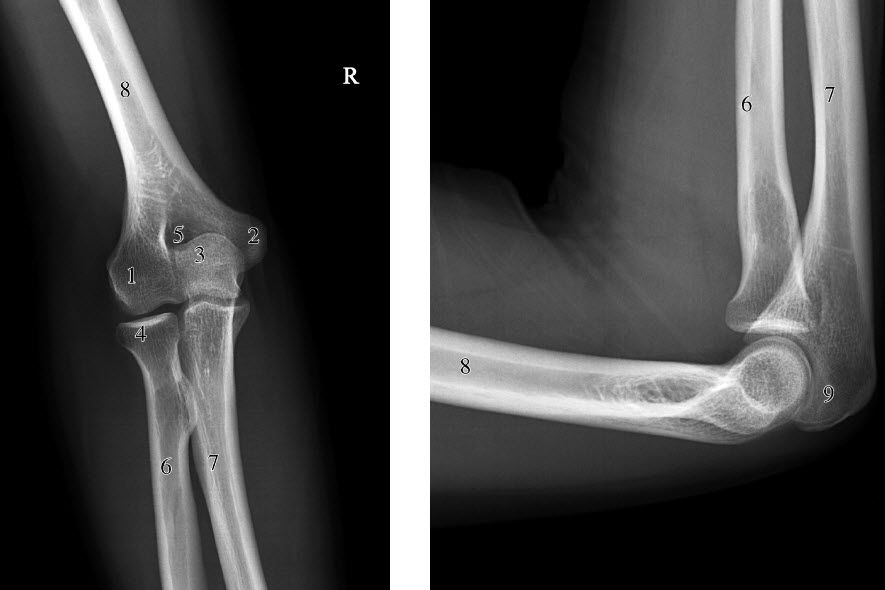
\includegraphics[width=6.73958in,height=3.32292in]{./images/Image00004.jpg}
\end{table}

\begin{table}[htbp]
\centering
\caption{引起昏迷的全身性疾病及其分类、发病机制和常见病因}
\label{tab2-2}
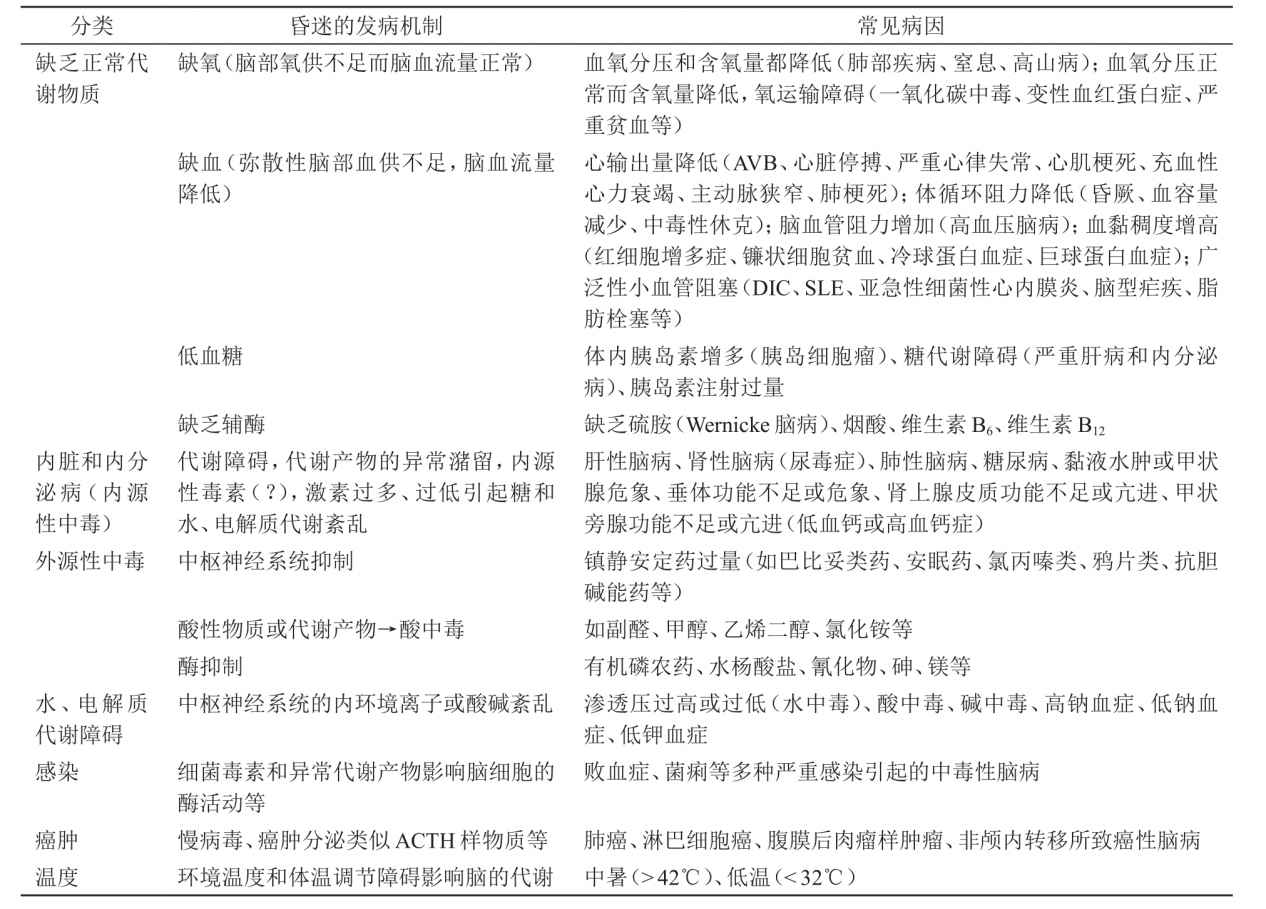
\includegraphics[width=6.73958in,height=4.83333in]{./images/Image00005.jpg}
\end{table}

\paragraph{脉搏}

脉搏触诊有助于及时发现急性心源性脑缺血综合征。脉慢而洪大见于脑出血、酒精中毒;脑脓肿患者的脉搏常缓慢、充实而规则;而脑膜炎患者的脉搏多细速。颠茄类、氯丙嗪中毒时脉搏显著增快。脉搏先慢后快,同时伴有血压下降者,可见于脑疝压迫脑干、延髓生命中枢衰竭,提示预后不良。

\paragraph{呼吸}

观察患者的呼吸方式、节律和频率等。呼吸深而快,常见于代谢性酸中毒(糖尿病、尿毒症等);鼾声呼吸且伴有呼吸时一侧面肌瘫痪者提示脑出血。浅而快速的规律性呼吸见于休克、心肺疾患或镇静催眠药中毒引起的呼吸衰竭,肺炎等缺氧性疾病可伴发绀和鼻翼扇动;呼吸深而慢、同时脉搏慢而有力和血压增高,为颅内压增高的表现。呼吸过慢并伴有叹息样呼吸常为吗啡类药物中毒。呼气带有氨味见于尿毒症昏迷;带有苹果味见于糖尿病昏迷;苦杏仁气味提示氢氰酸(苦杏仁、木薯、氰化物等)中毒;呈酒味提示酒精中毒;呼气及排泄物有大蒜样臭味可见于有机磷农药中毒;呼气中及尿液出现“肝臭”者提示肝性脑病。

昏迷患者呼吸节律的异常类型常常提示脑部病变的部位,与神经功能障碍水平定位有密切关系。双侧额叶损害可出现过度换气后呼吸暂停(PHVA)现象,即每在5~10次深呼吸后呼吸暂停。脑部广泛病损使中脑内呼吸中枢失去大脑的控制时,可出现潮式呼吸,即陈-施呼吸(Cheyne-Stokes
respiration,CSR),表现为呼吸由浅慢逐渐变为深快,再由深快变为浅慢,随后出现一段呼吸暂停后,然后重复上述周期性呼吸。潮式呼吸的周期可以长达30秒~2分钟,暂停时间可长达5~30秒。当中脑和脑桥上部功能受损后,可出现中枢神经源性过度呼吸(central
neurogenic
hyperventilation,CNH),呼吸深、快、均匀、持久,频率达40~70次/分。脑桥下部损害后可出现:①喘息样呼吸(gasping
of
breaths),常在濒死时出现,表现为深呼吸、较慢的频率,跳跃式深吸气,呼吸暂停6~10秒,可见于延髓内肿瘤或严重的药物中毒时;②交替呼吸,表现为一次强呼吸和一次弱呼吸交替;③间歇(Biot)呼吸,表现为每3~4次呼吸后出现呼吸暂停;④长吸式呼吸(apneustic
breathing),是一种吸气持续的延长性吸气痉挛,吸2~3次呼1次或吸足气后呼吸暂停。所谓鱼嘴式呼吸(每次吸气时下颌张开似鱼嘴),亦见于脑干下部损害时,常为预后严重的征兆。延髓受损时,呼吸紊乱更为严重,频率和幅度均不时改变,间以不规则地呼吸中断,有人亦称其为“共济失调性呼吸”(ataxic
breathing),最后发展至呼吸完全停止。在天幕上占位病变发展至出现天幕裂孔疝和枕大孔疝的过程中,有时可见到呼吸形式的一系列改变(潮式呼吸→中枢神经源性过度呼吸→喘息式呼吸→共济失调性呼吸),提示脑干功能自首端向尾端逐渐发生障碍。

\paragraph{血压}

血压显著增高,见于脑出血、高血压脑病、颅内压增高等;血压过低常见于糖尿病昏迷、酒精中毒、巴比妥类药物中毒等。

\paragraph{皮肤黏膜}

皮肤灼热干燥见于中暑高热;皮肤湿润多汗见于低血糖昏迷、有机磷农药中毒等;皮肤苍白常见于尿毒症性、低血糖性昏迷等;皮肤潮红见于脑出血、颠茄类中毒及酒精中毒;口唇发绀为严重缺氧如窒息、自缢或肺性脑病等;口唇樱红考虑一氧化碳中毒、严重酸中毒;口角见到单纯疱疹,考虑为疱疹性脑炎、脑型疟疾、大叶性肺炎或流脑等;皮肤巩膜黄染应考虑肝性脑病或药物中毒;昏迷伴有结合膜瘀斑、皮疹、皮肤瘀斑,须鉴别脓毒症、流脑、流行性出血热等引起的昏迷;有无头部、颜面部皮肤损伤的痕迹,有无舌咬伤、耳鼻部出血、脑脊液漏、耳后及皮下出血等,对诊断颅骨骨折、颅脑外伤及癫痫大发作常有帮助;颈部手术瘢痕可能提示甲状腺或甲状旁腺疾患,电解质不平衡或内分泌功能障碍;胸腔手术或乳房手术瘢痕应想到颅内转移或伴随于恶性肿瘤的高钙血症、低钠血症等电解质紊乱。应注意肢体、皮肤上成串的针疤或皮下脓肿可能曾滥用药物。

\hypertarget{text00010.htmlux5cux23CHP1-2-2-1-3}{}
(三) 神经系统检查

意识障碍时神经系统查体主要包括以下几个方面的检查
:眼征、对疼痛刺激的反应、瘫痪体征、脑干反射、锥体束征和脑膜刺激征等。

\paragraph{眼征}

包括以下几个方面:

\hypertarget{text00010.htmlux5cux23CHP1-2-2-1-3-1-1}{}
(1) 瞳孔变化:

观察瞳孔的大小、形状、位置、双侧对称性及对光反应,可帮助判断神经损害的部位及程度。①瞳孔对光反射:为光线刺激瞳孔引起的缩瞳反射。其传导径路为:视网膜→视神经→中脑被盖前区→埃-魏核→动眼神经→膝状神经节→颈上交感神经节节后纤维→瞳孔括约肌,径路上任何一处损害均可引起对光反射丧失和瞳孔散大。瞳孔对光反射与昏迷程度成正比(但巴比妥类中毒虽呈深昏迷,对光反射却残存是特征)。②瞳孔改变与病因:单侧瞳孔扩大,除外药物作用,昏迷患者单侧瞳孔扩大(≥5mm)者,可定为视神经损害或动眼神经损害造成。视神经损害常由于急性颅脑外伤伴发视神经损伤,有球后视神经炎过去史,或局部肿瘤或动脉瘤压迫引起单侧性黑矇性瞳孔麻痹,同侧直接光反射及对侧间接光反射消失;视神经萎缩者,亦可见该侧瞳孔扩大。动眼神经损害单侧瞳孔扩大,多见于后交通动脉瘤破裂引起的蛛网膜下腔出血,也可见于颞叶钩回疝、颅脑外伤伴发硬膜外血肿、脑出血、脑肿瘤等压迫。颈内动脉血栓形成,大脑中动脉浅支或深支梗塞时,亦可见单侧瞳孔扩大。个别癫痫患者抽搐后出现暂时性单侧瞳孔扩大,机制不明。双侧瞳孔扩大,可见于药物或食物中毒如颠茄类、巴比妥类(有时缩小)、氰化物、肉毒杆菌中毒等;脑疝进行到晚期瞳孔由单侧扩大扩展为双侧扩大,昏迷加深,提示预后不良。天幕上病变尚未引起脑疝或中脑结构移位时,瞳孔大小接近正常,若发生小脑幕切迹疝,则见病灶侧瞳孔扩大,对光反射消失,若观察脑疝形成的全过程,则可发现扩大侧瞳孔先有缩小的改变(由于动眼神经的压迫与牵拉,病侧缩瞳纤维首先受到刺激,继而麻痹)。单侧瞳孔缩小较少见,上述幕上占位病变导致早期颞叶钩回疝时,可见同侧瞳孔缩小,而光反射存在;脑干梗死也可见到一侧瞳孔缩小(霍纳综合征表现之一)。双侧瞳孔缩小,可见于氯丙嗪、吗啡类药物、有机磷农药、水合氯醛、毒蕈等中毒与尿毒症;双侧瞳孔缩小如针眼,伴有高热是原发性脑桥出血的特征,若患者还有四肢阵发性强直性抽搐则是脑室出血的表现。中央型间脑疝而致双侧下丘脑损害可出现双侧瞳孔缩小。

\hypertarget{text00010.htmlux5cux23CHP1-2-2-1-3-1-2}{}
(2) 眼球运动:

眼球运动受大脑皮质、脑桥、中脑和第3、4、6脑神经控制,其运动异常有重要的定位意义。在代谢性脑病中,仅巴比妥类和苯妥英钠中毒可有眼球运动障碍。若患者的眼球和浅睡眠一样,能缓慢地向两侧转动,说明脑桥和中脑的有关功能尚相对地完好,据此可推测天幕下病变引起的昏迷可能性较小。一侧大脑半球有较广泛的损害时,患者双眼常偏向瘫痪肢体的对侧;一侧脑桥受损时,则双眼偏向肢体瘫痪的同侧。在双侧大脑皮质急性病变时,可见到有眼球激动现象,每隔几秒钟双眼出现强烈的快速摆动。丘脑底部和上位中脑损害患者,眼球可能向下和向内转,就像盯着自己鼻尖看。眼球浮动(ocular
bobbing)是双眼球快速同向下转后又缓慢地向上转恢复至原位,每分钟重复2~3次,转动的幅度约1~3mm,它发生于眼球水平向运动机制被破坏的情况,其机制为脑桥侧视中枢受损,而中脑的眼球垂直运动中枢未受损之故,见于脑桥的双侧性损害。脑干广泛严重损害时,眼球运动完全丧失而固定在正中位。垂直性眼球运动障碍如双眼向上或向下凝视,提示中脑四叠体附近或下丘脑病变;分离性眼球运动可为小脑损害表现。

\hypertarget{text00010.htmlux5cux23CHP1-2-2-1-3-1-3}{}
(3) 眼底检查:

凡是能引起颅内压增高的疾病均可引起眼底改变。颅脑外伤或颅内出血后12~24小时即可出现视神经乳头水肿的变化;但严重的视乳头水肿多数是由于长期颅内压增高的后果,应考虑有脑肿瘤、脑脓肿等占位病变的可能。如视网膜有广泛的渗出物、出血,则应考虑有糖尿病、尿毒症、高血压脑病等可能。玻璃体下较大的或视网膜广泛的浅表出血通常见于蛛网膜下腔出血。

\paragraph{对疼痛刺激的反应}

用力按压眶上缘、胸骨检查昏迷患者对疼痛的运动反应,有助于定位脑功能障碍水平或判断昏迷的程度。出现单侧或不对称性姿势反应时,健侧上肢可见防御反应,病侧则无,提示瘫痪对侧大脑半球或脑干病变。观察面部疼痛表情时,可根据面肌运动,判断有无面瘫。疼痛引起去皮质强直(decorticate
rigidity),表现为上肢内收和屈曲,下肢伸直,与丘脑或大脑半球病变有关;去脑强直(decerebrate
rigidity)表现为四肢伸直,肌张力增高或角弓反张,提示中脑功能受损,较去皮质强直脑功能障碍程度更为严重。脑桥和延髓病变患者通常对疼痛无反应,偶可发现膝部屈曲(脊髓反射)。

\paragraph{瘫痪体征}

意识障碍和昏迷患者的瘫痪检查,可通过疼痛刺激观察面部表情与肢体活动,以及肢体坠落试验等来判定。①观察面颊:一侧面瘫时,可见该侧鼻唇沟变浅,口角低垂,睑裂增宽,呼气时面颊鼓起,吸气时面颊塌陷,呈吸烟斗动作。②疼痛刺激:压迫眶上切迹或捏掐肢体,观察患者肢体活动情况,瘫痪侧少动或不动。③观察双眼球共同偏视(见前述)。④胸骨反射:针刺胸骨柄部,引起一侧或双侧上肢的屈曲反应,手移向胸骨部,刺激加重,可波及下肢。一侧肢体反射消失或运动反应弱,提示该侧肢体瘫痪。⑤上肢坠落试验:将患者双上肢抬起,使与躯干呈垂直位,突然放手,观察肢体坠落情况,瘫痪肢体迅速坠落而且沉重,无瘫痪肢体则向外侧倾倒,缓慢坠落。⑥下肢坠落试验:将患者下肢膝部屈曲抬高,足跟着床,突然松手时,瘫痪侧肢体不能自动伸直,并向外侧倾倒;无瘫痪肢体则呈弹跳式伸直,并能保持足垂直位。⑦足外旋试验:先将患者的双下肢伸直放平,然后把双足扶直并拢,突然松开时,则瘫痪肢体的足立刻外旋倾倒,足外缘着床;无瘫痪的足,仍能维持足垂直位。⑧反射的改变:瘫痪肢体侧常伴有中枢性面瘫,腹壁、提睾反射减弱或消失,腱反射增强,病理反射阳性。

\paragraph{脑干反射}

可通过睫脊反射(ciliospinal reflex)、角膜反射(corneal
reflex)、头眼反射(oculocephalic reflex)和眼前庭反射(oculovestibular
reflex)等脑干反射来判断是否存在脑干功能损害。反射性眼球运动包括头眼反射和眼前庭反射。

\hypertarget{text00010.htmlux5cux23CHP1-2-2-1-3-4-1}{}
(1) 睫脊反射:

给予颈部皮肤疼痛刺激时可引起双侧瞳孔散大,此反射存在提示下位脑干、颈髓、上胸段脊髓及颈交感神经功能正常。

\hypertarget{text00010.htmlux5cux23CHP1-2-2-1-3-4-2}{}
(2) 角膜反射:

角膜反射是由三叉神经的眼神经与面神经共同完成的,当三叉神经的第一支(眼神经)或面神经损害时,均可出现角膜反射消失。若脑桥上部和中脑未受累及,角膜反射存在;一侧角膜反射消失见于同侧面神经病变(同侧脑桥),双角膜反射消失见于一侧三叉神经受损或双侧面神经受损,提示中脑或脑桥受累,常有意识障碍。

\hypertarget{text00010.htmlux5cux23CHP1-2-2-1-3-4-3}{}
(3) 头眼反射:

又称玩偶眼试验(Doll's eye
test)。在浅昏迷患者,检查者使其眼睑睁开,并将患者的头向两侧或前后转动,先慢后快,患者双眼反射地朝与头转动相反的方向转动(如头转向右侧时,双眼凝视偏向左侧),谓之头眼反射(本体觉转头反射、环偶眼现象)阳性。在婴儿为正常反射,随着大脑发育而抑制。头眼反射的刺激主要通过颈部肌肉本体觉,通过本体觉神经纤维进入脊髓,先经过颈髓2~4节段的背根,然后进入颈髓再上升达到延髓前庭神经核、中脑顶盖部、脑桥,以及第3、4、6脑神经。正常人清醒状态下,头眼反射为大脑半球发起的视觉固定(或注视,visual
fixation)所抑制,故正常人头眼反射不存在。在嗜睡患者,开始2或3次转头可能引起相反的同向眼动,以后由于转头动作通常使患者觉醒而头眼反射消失。此反射在大脑半球弥漫性病变和间脑病变所致昏迷时出现并加强;脑干病变时此反射消失,如一侧脑干病变,头向该侧转动时无反射,向对侧仍存在。应强调的是:在怀疑有颈椎脱位与骨折可能的患者,绝对禁忌作此项检查。

\hypertarget{text00010.htmlux5cux23CHP1-2-2-1-3-4-4}{}
(4) 眼前庭反射:

或称冷热水试验。用注射器向一侧外耳道注入1ml冰水,大脑半球弥漫性病变而脑干功能正常时,出现双眼向冰水灌注侧强直性同向运动;昏迷患者,如存在完全的反射性眼球运动,提示脑桥至中脑水平的脑干功能完好;中脑病变时,眼前庭检查可显示灌注对侧眼球内收不能,同侧眼外展正常;脑桥病变时反应完全丧失。

\paragraph{脑膜刺激征}

脑膜刺激征包括颈强直(简称颈强)、Kernig征(凯尔尼格征)和Brudzinski征(布鲁津斯基征)等。颈上节段的脊神经根受刺激引起颈强直,腰骶节段的脊神经根受刺激,则出现Kernig征和Brudzinski征。阳性提示有脑膜炎、蛛网膜下腔出血、脑炎、脑水肿及颅内压增高等的可能。深昏迷时脑膜刺激征可消失。检查方法包括:

\hypertarget{text00010.htmlux5cux23CHP1-2-2-1-3-5-1}{}
(1) 屈颈试验:

患者仰卧,检查者托患者枕部并使其头部前屈而表现不同程度的颈强,被动屈颈受限,称为颈强直,但需排除颈椎病。正常人屈颈时下颏可触及胸骨柄,部分老年人及肥胖者除外。

\hypertarget{text00010.htmlux5cux23CHP1-2-2-1-3-5-2}{}
(2) Kernig征:

患者仰卧,下肢于髋、膝关节处屈曲成直角,检查者于膝关节处试行伸直小腿,如伸直受限并出现疼痛,大、小腿间夹角<
135°,为Kernig征阳性。如颈强(+)而Kernig征(−),称为颈强-Kernig征分离,见于后颅窝占位性病变和小脑扁桃体疝等。

\hypertarget{text00010.htmlux5cux23CHP1-2-2-1-3-5-3}{}
(3) Brudzinski征:

患者仰卧屈颈时出现双侧髋、膝部屈曲;一侧下肢膝关节屈曲位,检查者使该侧下肢向腹部屈曲,对侧下肢亦发生屈曲(下肢征),均为Brudzinski征阳性。

\paragraph{反射检查}

一般认为,浅反射由减退至消失而同时深反射由亢进至消失,均提示昏迷的程度加深。常用的深反射(为肌腱和关节反射)有肱二头肌、肱三头肌反射,桡骨膜反射,膝反射,跟腱反射等;常用的浅反射(浅反射是刺激皮肤、黏膜、角膜等引起肌肉快速收缩反应)有角膜反射、咽反射、腹壁反射、提睾反射、跖反射、肛门反射等。常用的病理反射有:

\hypertarget{text00010.htmlux5cux23CHP1-2-2-1-3-6-1}{}
(1) 巴宾斯基征(Babinski征):

是经典的病理反射,提示锥体束受损。用竹签轻划足底外侧,自足跟向前至小趾根部足掌时转向内侧,阳性反应为趾背屈,可伴其他足趾扇形展开。

\hypertarget{text00010.htmlux5cux23CHP1-2-2-1-3-6-2}{}
(2) 巴宾斯基等位征:

包括:①Chaddock征:由外踝下方向前划至足背外侧;②Oppenheim征:用拇指和示指沿胫骨前缘自上而下用力下滑;③Schaeffer征:用手挤压跟腱;④Gordon征:用手挤压腓肠肌;⑤Gonda征:用力下压第4、5足趾,数分钟后突然放松;⑥Pussep征:轻划足背外侧缘。阳性反应均为趾背屈。临床意义一般认为同Babinski征。

\hypertarget{text00010.htmlux5cux23CHP1-2-2-1-3-6-3}{}
(3) 强握反射:

指检查者用手指触摸患者手掌时被强直性握住的一种反射。新生儿为正常反射,成人见于对侧额叶运动前区病变。

\hypertarget{text00010.htmlux5cux23CHP1-2-2-1-3-6-4}{}
(4) 脊髓自主反射:

脊髓横贯性病变时,针刺病变平面以下皮肤引起单侧或双侧髋、膝、踝部屈曲(三短反射)和Babinski征阳性。若双侧屈曲并伴腹肌收缩、膀胱及直肠排空,以及病变以下竖毛、出汗、皮肤发红等,称为总体反射。

对于昏迷患者除重点注意以上项目外,尚应注意胸、腹部体征如昏迷偏瘫患者伴有心脏杂音,心房纤颤,考虑心脏病伴有脑梗死;昏迷、抽搐伴有心音片刻听不到,考虑阿-斯综合征;昏迷、休克、肺部啰音等,考虑中毒性肺炎;昏迷患者伴腹水、肝脾大或缩小,常提示肝性脑病、血液病、细菌性心内膜炎、脓毒症等可能性。

实验室检查与特殊检查应根据需要选择进行,但除三大常规外,对于意识障碍和昏迷患者,血清电解质、尿素氮(BUN)、CO\textsubscript{2}
CP、血糖等应列为常规检查;对病情不允许者必须先就地抢救,视病情许可后再进行补充。脑电图、头颅CT和MRI,以及脑脊液检查对昏迷的病因鉴别有重要意义。

在通过上述病史询问,体检,神经系统检查及必要的有关辅助检查后,一般可依下列顺序对意识障碍与昏迷进行诊断和鉴别诊断。

\subsubsection{判断是否为意识障碍和昏迷}

临床上判断是否属于意识障碍和昏迷一般不难,但首先应排除下述两种情况:

\paragraph{几种特殊类型的意识障碍}

\hypertarget{text00010.htmlux5cux23CHP1-2-2-2-1-1}{}
(1) 去皮质综合征(decorticate syndrome):

也称去大脑皮质状态(apallic
state),是由于双侧大脑皮质发生弥散性的严重损害而导致大脑皮质功能减退或丧失,皮质下功能仍保存。其特点是皮质与脑干的功能出现分离现象:大脑皮质功能丧失,对外界刺激无任何意识反应,不言不语;而脑干各部分的功能正常:患者眼睑开闭自如,常睁眼凝视(即醒状昏迷),痛觉灵敏(对疼痛刺激有痛苦表情及逃避反应),角膜与瞳孔对光反射均正常。四肢肌张力增高,双上肢常屈曲,双下肢伸直(去皮质强直),大小便失禁,还可出现吸吮反射及强握反射,甚至伴有手足徐动、震颤、舞蹈样运动等不随意运动。该综合征常见于缺氧性脑病、脑炎、中毒和严重颅脑外伤等。

\hypertarget{text00010.htmlux5cux23CHP1-2-2-2-1-2}{}
(2) 无动性缄默症(akinetic mutism):

又称睁眼昏迷(coma
vigil),由脑干上部和丘脑的ARAS受损引起,此时大脑半球及其传出通路无病变。患者能注视周围环境及人物,貌似清醒,但不能活动或言语,二便失禁。肌张力减低,无锥体束征。强烈刺激不能改变其意识状态,存在觉醒-睡眠周期。本症常见于脑干梗死。

\hypertarget{text00010.htmlux5cux23CHP1-2-2-2-1-3}{}
(3) 植物状态(vegetative state):

是指大脑半球严重受损而脑干功能相对保留的一种状态。表现为对自身和外界的认知功能完全丧失,能睁眼,有睡眠和觉醒周期,可有无意义哭笑,二便失禁。肢体可有无意识的随意运动,脑干反射存在。持续性植物状态指颅脑外伤后植物状态持续12个月以上,其他原因持续3个月以上。

\paragraph{神经精神疾病所致的几种貌似昏迷状态}

\hypertarget{text00010.htmlux5cux23CHP1-2-2-2-2-1}{}
(1) 精神抑制状态(depression state):

常见于强烈精神刺激后或癔症性昏睡发作,患者表现出僵卧不语,对外界刺激如呼唤、推摇,甚至疼痛刺激常不发生反应。双目紧闭,扳开眼睑时有明显抵抗感,并见眼球向上翻动,放开后双眼迅速紧闭。瞳孔大小正常,光反应灵敏,眼脑反射正常,无病理反射。脑电图呈觉醒反应,经适当治疗可迅速复常。癔症性昏睡,多数尚有呼吸急促,也有屏气变慢,检查四肢肌张力增高,对被动活动多有抵抗,有时四肢伸直、屈曲或挣扎、乱动。常呈阵发性,多属一过性病程,在暗示治疗后可迅速恢复。

\hypertarget{text00010.htmlux5cux23CHP1-2-2-2-2-2}{}
(2) 木僵(stupor):

表现为不语不动,不饮不食,对外界刺激缺乏反应,甚至出现大小便潴留,多伴有蜡样屈曲和违拗症,言语刺激触及其痛处时可有流泪、心率增快等情感反应,缓解后多能清楚回忆发病过程。见于精神分裂症的紧张性木僵、严重抑郁症的抑郁性木僵、反应性精神障碍的反应性木僵等。

\hypertarget{text00010.htmlux5cux23CHP1-2-2-2-2-3}{}
(3) 闭锁综合征(locked-in syndrome):

又称去传出状态(deefferented
state)。病变位于脑桥基底部,双侧锥体束和皮质脑干束均受累。患者意识清醒,因运动传出通路几乎完全受损而呈失运动状态,除尚有部分眼球运动外,呈现四肢瘫,不能说话和吞咽,表情缺乏,就像全身被闭锁,但可理解语言和动作,能以睁闭或眼垂直运动示意。当临床怀疑本症时,可让患者“睁开你的眼睛”、“向上看”、“向下看”和“看你的鼻尖”等,可作出鉴别。

\hypertarget{text00010.htmlux5cux23CHP1-2-2-2-2-4}{}
(4) 意志缺乏症(abulia):

患者处于清醒状态,运动感觉功能存在,但因缺乏始动性而不语不动,对刺激无反应,无欲望,呈严重淡漠状态,可有额叶释放反射,如掌颏反射、吸吮反射等。本症多由双侧额叶病变所致。

\hypertarget{text00010.htmlux5cux23CHP1-2-2-2-2-5}{}
(5) 失语(aphasia):

程度较重的失语患者,特别是伴有嗜睡、瘫痪时,对外界刺激失去反应能力而易被误认为昏迷。如系失语而非昏迷的患者,对声、光、疼痛刺激的反应是灵敏的;对言语以外的示意性动作、表情等仍能领会、理解,而有适当的表情反应,或喃喃发声,欲语不能。

\subsubsection{意识障碍和昏迷程度的评定}

临床上除将意识障碍分为嗜睡、昏睡、浅昏迷、中昏迷和深昏迷五级(见前述)外,常用格拉斯哥昏迷计分法(Glasgow
coma
scale,GCS)。GCS是以睁眼(觉醒水平)、言语(意识内容)和运动反应(病损平面)三项指标的15项检查结果来判断患者昏迷和意识障碍的程度,见表\ref{tab2-3}。以上三项检查共计15分。GCS分值愈低,脑损害的程度愈重,预后亦愈差。但此量表有一定局限性:对眼肌麻痹、眼睑肿胀者不能评价其睁眼反应,对气管插管或切开者不能评价其言语活动,四肢瘫患者不能评价其运动反应。1978年此量表被修订为Glasgow-Pittsburgh量表,增加了对光反射、脑干反射、抽搐情况和自发性呼吸四大类检查,见表\ref{tab2-4}。合计为7项35级,最高为35分,最低为7分。在颅脑损伤中,35~28分为轻型,27~21分为中型,20~15分为重型,14~7分为特重型颅脑损伤。该观察表即可判定昏迷程度,也反映了脑功能受损水平。

\subsubsection{意识障碍和昏迷的病因诊断}

意识障碍和昏迷的病因诊断极其重要。通常必须依据病史、体格和神经系统检查,以及有关的辅助检查资料,经过综合分析,能查出导致昏迷的原发病因。由于昏迷的病因众多,而且某些病例的病程进展甚快,病情危重或因条件所限,无法进行详细或特殊的辅助检查,使病因诊断受到影响。但以下诊断思路具有较大的临床价值。

\hypertarget{text00010.htmlux5cux23CHP1-2-2-4-1}{}
(一) 确定是颅内疾病抑或全身性疾病

通常先确定是颅内疾病抑或全身性疾病
,如确定意识障碍和昏迷是颅内病变引起,尚需进一步确定是颅内局限性病变抑或弥散性病变,如是前者,它是位于幕上抑或幕下,具体病因是什么。

\paragraph{颅内疾病}

位于颅内的原发性病变,在临床上通常先有大脑或脑干受损的定位症状和体征,较早出现意识障碍和精神症状,伴明显的颅内高压症和脑膜刺激征,提示颅内病变的有关辅助检查如脑脊液检查、CT扫描等常有阳性发现。临床上可根据神经系统体征基本上将表现分为两类:①主要呈现局限性神经体征,如脑神经损害、肢体瘫痪、局限性抽搐、偏侧锥体束征等,常见于脑出血、梗死、脑炎、外伤、占位性病变等;②主要表现为脑膜刺激征而无局限性神经体征,最多见于脑膜炎、蛛网膜下腔出血等。

\begin{table}[htbp]
\centering
\caption{GCS昏迷评定量表}
\label{tab2-3}
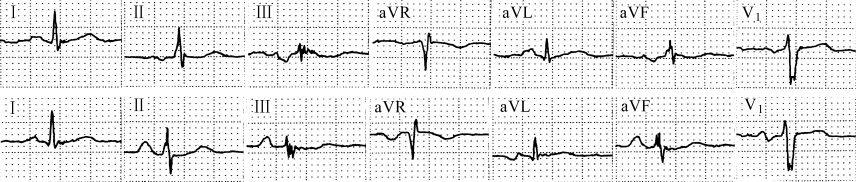
\includegraphics[width=6.66667in,height=2.03125in]{./images/Image00006.jpg}
\end{table}

\begin{table}[htbp]
\centering
\caption{Glasgow-Pittsburgh昏迷观察表}
\label{tab2-4}
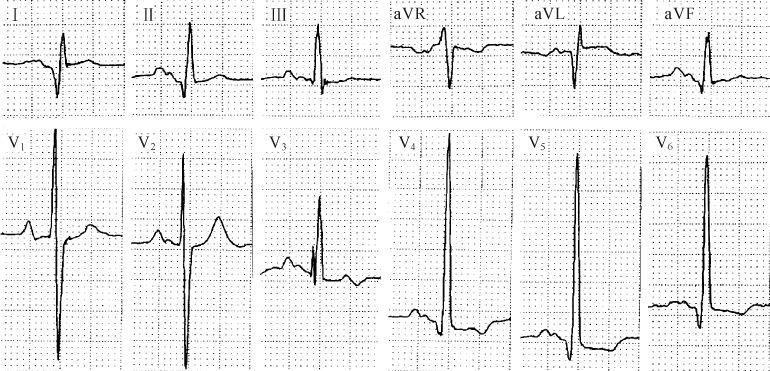
\includegraphics[width=6.69792in,height=4.21875in]{./images/Image00007.jpg}
\end{table}

如确定昏迷是颅内病变引起,尚可将颅内病变又进一步区分为颅内幕上局限性病变、幕下局限性病变和颅内弥散性病变三组。它们的特征参见表\ref{tab2-1}。

\paragraph{全身性疾病}

全身性疾病可影响脑代谢而引起弥散性脑损害,又称代谢性脑病。同原发性颅内病变相比,其临床特点为:先有颅外器官原发病的症状和体征,以及相应的实验室检查阳性发现,后才出现脑部受损的征象。由于脑部损害为非特异性或仅是弥散性功能抑制,临床上一般无持久性和明显的局限性神经体征和脑膜刺激征,主要是多灶性神经功能缺乏的症状和体征,且大都较对称;通常先有精神异常,意识内容减少。一般是注意力减退,记忆和定向障碍,计算和判断力降低,尚有错觉、幻觉,随病程进展,意识障碍加深。此后有的可出现不同层次结构损害的神经体征,如昏迷较深和代谢性呼吸抑制很严重,而眼球运动和瞳孔受累却相对较轻。脑脊液改变不显著,颅脑CT扫描等检查无特殊改变,不能发现定位病灶。其病因很多,它们的特征参见表\ref{tab2-2}。

\hypertarget{text00010.htmlux5cux23CHP1-2-2-4-2}{}
(二) 根据患者是否伴有脑膜刺激征和脑局灶体征来判断昏迷的病因

\paragraph{脑膜刺激征(+)而脑局灶性体征(−)}

\hypertarget{text00010.htmlux5cux23CHP1-2-2-4-2-1-1}{}
(1) 突发剧烈头痛:

蛛网膜下腔出血(脑动脉瘤、脑动静脉畸形破裂)。

\hypertarget{text00010.htmlux5cux23CHP1-2-2-4-2-1-2}{}
(2) 急性发病、发热在先:

化脓性脑膜炎、乙型脑炎、其他急性脑炎等。

\hypertarget{text00010.htmlux5cux23CHP1-2-2-4-2-1-3}{}
(3) 亚急性或慢性发病:

真菌性、结核性、癌性脑膜炎。

\paragraph{脑膜刺激征(−)而脑局灶性体征(+)}

\hypertarget{text00010.htmlux5cux23CHP1-2-2-4-2-2-1}{}
(1) 突然起病者:

如脑出血、脑栓塞、脑梗死等。

\hypertarget{text00010.htmlux5cux23CHP1-2-2-4-2-2-2}{}
(2) 以发热为前驱症状:

如脑脓肿、血栓性静脉炎、各种脑炎、急性播散性脑脊髓炎、急性出血性白质脑病等。

\hypertarget{text00010.htmlux5cux23CHP1-2-2-4-2-2-3}{}
(3) 与外伤有关:

如脑挫伤、硬膜外血肿、硬膜下血肿等。

\hypertarget{text00010.htmlux5cux23CHP1-2-2-4-2-2-4}{}
(4) 缓慢起病、颅内压增高者:

脑肿瘤、慢性硬膜下血肿、脑寄生虫病等。

\paragraph{脑膜刺激征(−)和脑局灶性体征(−)}

\hypertarget{text00010.htmlux5cux23CHP1-2-2-4-2-3-1}{}
(1) 有明确中毒原因:

如酒精、麻醉药、安眠药、一氧化碳中毒等。

\hypertarget{text00010.htmlux5cux23CHP1-2-2-4-2-3-2}{}
(2) 尿检异常:

尿毒症、糖尿病、急性尿卟啉症等。

\hypertarget{text00010.htmlux5cux23CHP1-2-2-4-2-3-3}{}
(3) 休克状态:

低血糖、心肌梗死、肺栓塞、大出血等。

\hypertarget{text00010.htmlux5cux23CHP1-2-2-4-2-3-4}{}
(4) 有黄疸:

肝性脑病等。

\hypertarget{text00010.htmlux5cux23CHP1-2-2-4-2-3-5}{}
(5) 有发绀:

肺性脑病等。

\hypertarget{text00010.htmlux5cux23CHP1-2-2-4-2-3-6}{}
(6) 有高热:

重症感染、中暑、甲状腺危象等。

\hypertarget{text00010.htmlux5cux23CHP1-2-2-4-2-3-7}{}
(7) 体温过低:

休克、酒精中毒、黏液性水肿昏迷等。

\hypertarget{text00010.htmlux5cux23CHP1-2-2-4-2-3-8}{}
(8) 头部外伤:

脑震荡等。

\hypertarget{text00010.htmlux5cux23CHP1-2-2-4-2-3-9}{}
(9) 其他:

癫痫等。

\subsection{处理原则}

\paragraph{昏迷的最初处理}

常规措施有:①保持呼吸道通畅,氧疗,必要时气管插管或切开行人工呼吸。②维持循环功能,尽早开放静脉,建立输液通路(1~3个)。有休克应迅速扩充血容量,使用血管活性药物,尽快使收缩血压稳定在100mmHg左右。有心律失常者应予以纠正;有心肌收缩力减弱者应给予强心剂;心跳骤停时应立即行心肺复苏。③纳洛酮:常用剂量每次0.4~0.8mg,静脉注射或肌注,无反应可隔10~15分钟重复用药,直达预期效果;亦可用1.2~2.0mg加入250~500ml液体中静滴。

\paragraph{病因治疗}

针对病因采取及时果断措施是抢救成功的关键。若昏迷的病因已明确,则应迅速给予有效病因治疗。如由颅内占位性病变引起者,若条件许可应尽早作开颅手术,摘除肿瘤;细菌性脑膜脑炎引起者,应迅速给予大量而有效的抗生素治疗;因脑型疟疾而引起的昏迷,则可给盐酸奎宁0.5g置于5\%葡萄糖液250~500ml中静滴;由于低血糖引起者应立即给予高渗葡萄糖液;若为有机磷农药中毒所致者,应立即用胆碱酯酶复能剂和阿托品等特效解毒剂;糖尿病昏迷应予胰岛素治疗等。

\paragraph{对症支持疗法}

包括控制脑水肿、降低颅内压,维持水电解质平衡,镇静止痛,防治各种并发症(如急性心力衰竭、急性呼吸衰竭、消化道出血、急性肾功能衰竭、急性脑功能衰竭等)等,详见有关章节。

\protect\hypertarget{text00011.html}{}{}

\hypertarget{text00011.htmlux5cux23CHP1-2-4}{}
参 考 文 献

1. 张文武.急诊内科学.第2版.北京:人民卫生出版社,2007

2. 贾建平.神经病学.第6版.北京:人民卫生出版社,2008

3. Rowland LP. Merritt's Neurology. 11th ed. New York:Lippincott
Williams & Wilkins,2005

\protect\hypertarget{text00012.html}{}{}

\chapter{眩 晕}

眩晕是一主观症状,是机体对于空间关系的定向感觉障碍或平衡感觉障碍,是一种运动错觉,患者感外境或自身在旋转、移动或摇晃。在眩晕症状出现的同时,常伴有平衡失调、站立不稳、眼球震颤、指物偏向、恶心、呕吐、面色苍白、出汗及心率和血压的改变。

临床上可将眩晕分为前庭系统性眩晕(亦称真性眩晕)及非前庭系统性眩晕(亦称头晕)。前者由前庭神经系统病变(包括前庭末梢器、前庭神经及前庭的中枢连接)所引起,为真性眩晕,表现为有运动错觉的眩晕,例如自觉旋转、摇晃、移动感;后者常为头昏(头重脚轻、眼花、头脑昏昏沉沉、颅内在转动等诉说),但并无外境或自身旋转的运动觉,常由心血管系统疾病,全身中毒性、代谢性疾病,贫血,眼病等疾患所引起。

\subsection{病因与发病机制}

\subsubsection{病因分类}

眩晕的病因分类有多种方法,各家不甚统一,各有其优缺点。笔者认为根据神经系统疾病的诊断步骤先定位再定性的方法,较为实用,即根据病变的解剖部位及结合病因予以分类。现将常见的疾病列举如下:

\hypertarget{text00012.htmlux5cux23CHP1-3-1-1-1}{}
(一) 前庭系统性眩晕

包括前庭末梢感受器
、前庭神经、前庭诸核、内侧纵束、小脑、前庭皮质代表区之各种病损所产生的真性眩晕。

\paragraph{耳源性}

例如外耳道耵聍,急、慢性中耳炎,咽鼓管阻塞,鼓膜内陷,耳硬化症,迷路炎,慢性中耳炎内耳并发症(瘘管形成),梅尼埃病(Meniere
disease),运动病,良性位置性眩晕,迷路动脉血供障碍,内耳震荡等。

\paragraph{前庭神经病损}

前庭神经元炎、听神经鞘膜瘤、脑桥小角其他肿瘤、前庭神经炎、前庭神经外伤(岩锥骨折)或中毒性损害。

\paragraph{脑干病变}

脑桥、延髓的血管性和肿瘤性病变、脑干脑炎、多发性硬化、延髓空洞症、第四脑室肿瘤及囊肿。

\paragraph{小脑病变}

肿瘤、脓肿、出血及损伤。

\paragraph{大脑病变}

颞叶肿瘤或血管性病变,颞叶癫痫。

\paragraph{颈椎病变}

颈椎肥大性改变及颈椎间盘突出。

\hypertarget{text00012.htmlux5cux23CHP1-3-1-1-2}{}
(二) 非前庭系统性眩晕

1.眼性眩晕 如眼外肌麻痹、屈光不正、先天性视力障碍等。

2.心血管病变 如高血压、低血压、心律不齐、心力衰竭、大脑动脉硬化。

3.全身中毒性、代谢性、感染性疾病。

4.各种原因引起的贫血。

5.神经症。

\subsubsection{发病机制}

机体平衡的维持,定向功能的正常,是借视觉、本体觉(肌腱、关节中)及前庭平衡觉的协同作用而完成的,而后者对机体姿位平衡的维持更为重要。各种外界的刺激(信息),通过上述诸感受器如视觉、本体觉、前庭平衡觉传入至前庭核群、红核、网状结构、皮质下中枢、小脑等,不断反射性调节机体对各种姿位的平衡,各种加速度的反应,使机体在运动中与外界环境保持协调与平衡。神经冲动由皮质下中枢再向上传入大脑皮质,多数学者认为皮质平衡中枢在颞叶,Penfield为患者作脑部手术时,电刺激颞上回,引起“头晕”、“旋转”和“摇摆”感。应用电生理方法在动物实验中测定了前庭皮质投射区,罗猴的前庭皮质投射区位于第一体感区和第二体感区之间的中央后回,为Brodmann第2区稍后处。前庭的皮质投射似乎从感觉-运动皮质移向顶叶的联合皮质,皮质区接受两侧前庭投射。综上所述,皮质前庭代表区虽不甚确切,但一般认为在颞上回的后、上半部,颞顶交界处及岛叶的上部。丘脑后下腹核很可能为前庭传入的丘脑换元站。后下腹核位于后外侧腹核和后内侧腹核之间的底部。

前庭系统包括内耳迷路末梢感受器(半规管中的壶腹嵴、椭圆囊和球囊中的位觉斑),前庭神经、脑干中的前庭核群,小脑、内侧纵束、前庭脊髓束、前庭皮质代表区。三个半规管中的壶腹嵴,其感受器在半规管中内淋巴流动时接受角加速度的刺激,而椭圆囊、球囊的位觉斑则接受直线加速度、重力加速度的刺激,冲动沿着前庭神经传入中枢,反射性地调节机体平衡。在正常情况下,从前庭器官传入中枢的有关平衡觉的信息并不为人所感知,只是当前庭器官或其中枢连接受到较大刺激或病理性损害时,前庭感受的刺激(信息)与来自肌肉、关节的本体觉及视觉感受器的关于空间定向的冲动不一致时,于是产生眩晕,亦即运动错觉。由于前庭核通过内侧纵束与动眼神经核之间有密切的联系,因此当前庭感受器、前庭神经及前庭核群受到病理性刺激(或破坏)时常出现眼球震颤,这种前庭性眼球震颤的特点为眼球有一慢相与一快相交替的有规律的来回颤动。慢相系由前庭-动眼反射通路实现,偏向前庭兴奋性相对较低的一侧。快相则为皮质下中枢、脑干网状结构向相反方向调节眼球运动的现象。因快相容易观察,通常即以此代表眼震的方向,与眩晕的感觉方向一致。前庭诸核通过内侧纵束、前庭脊髓束及网状脊髓束、前庭→小脑→红核→脊髓等通路,与脊髓中的前角运动细胞相连接,所以前庭病变时或前庭器受到较大的刺激时,除出现眼震外还可出现躯体向一侧倾倒及肢体错定物位(指物偏向)等体征。前庭核还与脑干网状结构中的血管运动中枢、迷走神经核等连接,所以前庭器病变时在眩晕的同时常伴有恶心、呕吐、苍白、出汗甚至血压、呼吸、脉搏等改变。

\subsection{诊断思路}

眩晕是一主观症状,为了对眩晕病因作出正确的诊断与鉴别诊断,必须详询病史,细致的体格检查,必要的辅助检查,并应熟悉与了解常见引起眩晕疾病的特点。

\subsubsection{病史}

应详细了解眩晕的性质、程度、时间、诱发因素、伴随症状以及可能引起眩晕的有关病史(药物中毒、外伤史)及询问包括神经科、内科、耳鼻喉科的有关疾病。

\subsubsection{体格检查}

\paragraph{神经系统方面}

除一般的神经系统检查外,特别应注意有无自发性眼球震颤、共济失调、听力障碍及颅内压增高征。

\paragraph{内科方面}

应检查血压、心脏,有无高血压、低血压、心律不齐、心功能不全,有无贫血、全身感染、中毒、代谢紊乱等。

\paragraph{耳科方面}

应检查外耳道、鼓膜、中耳、鼻咽部,注意有无耵聍阻塞外耳道,有无表皮样瘤性中耳炎及耳硬化症。疑有迷路瘘管时应作瘘管试验。

\paragraph{听力学检查}

应用表、音叉试验法可以大致了解听力情况、听力障碍的性质(传导性、感音性)及程度,必要时作电测听检查,包括作短增量敏感指数(SISI)试验、复聪(recruitment)试验。

\paragraph{前庭功能检查}

包括自发性眼震、倾倒、指物偏向、变温(caloric)试验、旋转试验、直流电试验、位置试验、视动性眼震试验,必要时还需作眼震电图(ENG)检查。

\subsubsection{辅助检查}

可根据病情作必要的辅助检查,例如头颅X线摄片、乳突摄片、脑电图、经颅Doppler超声(TCD)检查、头颅CT扫描、头颅磁共振成像、疑为颈椎病者则需作颈椎摄片或颈椎CT扫描。疑有颅内炎症者需作腰穿检查脑脊液。

\subsubsection{前庭功能检查的临床意义}

前庭功能检查对于眩晕症的诊断有肯定的价值,有助于确定病损的部位,鉴别眩晕的性质。前庭系统性眩晕常有前庭功能异常,而非系统性眩晕则多数均无明显的前庭功能异常。前庭功能检查项目繁多,兹将这些检查的临床意义叙述如下。

\paragraph{自发性眼球震颤}

前庭系统性眩晕常伴有眼震,而非系统性眩晕一般均无自发性眼震。前庭周围性病变及前庭中枢性病变时所出现的自发性眼震的鉴别大致有如下几点:①前庭周围性:眼震常为一种方向,多为水平性,多呈突发性,伴有明显眩晕且与眼震程度一致,闭目后眩晕症状并不减轻,固视可使眼震减弱,眼震之快相通常为向病损的对侧。闭目时向前伸出的两个上肢偏向病损侧,躯体常向眼震的慢相倾倒。常伴有听力减退。眼震持续时间一般不超过3周。如梅尼埃病、急性迷路炎、急性前庭神经损伤等。②前庭中枢性:眼震方向不一,可为水平、旋转、垂直、斜向,持续时间较长。不一定伴有明显眩晕,眩晕与眼震程度不一致。过指和倾倒方向并不恒定,与眼震方向无肯定关系。可能无听力障碍。眼震常不能被固视抑制(减弱)。病变多数累及脑桥、延髓或小脑,因天幕上病变直接引起眼震者罕见。

至于眼源性眼震,其特点是眼震呈摆动性,尤其当眼球在正中位时,眼震呈对称钟摆样;眼球移向侧方时转为跳动样眼震,其快相向侧视方向;闭目时眼震消失;眼震持续时间长;不伴旋转性眩晕,若有诉“眩晕”,常觉为外境来回摆动或“眼花”,闭目后症状即消失,无听力障碍,无自发性倾倒。眼源性眼震可见于先天性白内障,先天性角膜云翳,白化病。眼震在幼小时即已存在,也偶然发生于成年后罹患的黄斑变性患者。

\paragraph{变温试验(caloric test)}

常用的方法是微量法或冷热交替法(Hall pike法)。其临床意义如下:

(1)
单侧功能减退或消失(半规管轻瘫或瘫痪)常指示该侧前庭器有病变。例如听神经瘤、梅尼埃病等。

(2)
一侧性前庭功能减退或消失并伴有持久的自发性眼球震颤,则病损已累及脑干或小脑。如脑桥小脑角占位性病变已侵犯及脑桥或小脑。

(3)
双侧性前庭功能减退:提示两侧前庭器(或前庭神经)病变,常见于中毒性病损(链霉素中毒)、感染性病损(前庭神经元炎或脑桥小脑角蛛网膜炎)。

(4)
变温试验反应消失而前庭直流电试验反应存在,提示病损位于前庭神经末梢器,例如迷路炎。

(5)
有自发性眼震及眩晕,但变温试验时诱发出的眩晕反应及迷走兴奋反应不明显,常提示病变位于颅后窝。

(6)
变温试验所诱发的眼震、眩晕、指物偏向,它们彼此在程度上、性质上有分离或不一致;诱发的眼震为反常性(眼震的性质错乱,如原应出现水平性眼震却出现垂直性)者或反向性(眼震与应出现的方向相反)者;变温试验时诱发的眼震只出现在慢相方向上的双眼偏斜而无明确的快相,均提示病变位于脑干。

(7)
前庭功能亢进:有两种情况:①单侧性亢进提示该侧前庭神经(前庭器)有刺激性病变存在,例如迷路炎的早期、梅尼埃病的初期;②双侧性亢进可能为神经症,是由于自主神经功能失调等因素所引起,亦可能由于颅内某些疾病使小脑对前庭的正常抑制作用减退、中枢前庭神经元兴奋性增高所引起,无定位价值。

(8)
用冷热交替法检查前庭功能,除可发现半规管功能是否正常、有无半规管麻痹(反应低下或消失),并可发现有无优势偏向。所谓优势偏向是指所诱发出的眼球震颤反应向一侧的眼震时程较向另一侧的眼震时程明显增大,例如以温水刺激右耳和以冷水刺激左耳均引起向右的眼球震颤。若这两个反应时程均大于使眼震向左的相应变温刺激反应时即称为向右的优势偏向。通常认为向一侧方向的眼震时程总和大于向对侧者的总和40秒以上者,即为有优势偏向。在椭圆囊及其与前庭神经核尾端部分连接的紧张性前庭机制发生病变时即可引起向对侧方向的优势偏向。但大脑颞叶后部病变时,有时亦可发现有朝向病侧的优势偏向。

\paragraph{位置试验}

眩晕患者,尤其是其眩晕症状的发生与头部处于某种特定位置有关者(此种眩晕可称位置性眩晕),作位置试验有一定的临床诊断价值。通过检查可以了解眩晕出现时是否同时伴有眼震,并可进一步鉴别此种位置性眩晕、位置性眼震系由前庭周围性病变抑或中枢性病变所引起。

位置性眩晕与位置性眼球震颤的检查方法:①嘱患者坐于检查桌上,观察其有无自发性眼震。②检查者立于患者的右侧,嘱患者头向右侧偏转45°,躯体亦向右侧轻度偏转,检查者用两手扶住患者的头部,然后嘱患者迅速躺下,头仍维持于向右侧偏转的位置。事先作为测试让患者躺下后头部超过检查台一端并悬垂于检查台沿之外。检查者始终用两手扶持其头部,以维持其头部向右侧偏转的位置,观察有无眩晕症状及眼球震颤。观察15秒如无眩晕症状及眼震出现,则让患者恢复原先坐位,亦观察15秒,注意有无眩晕与眼震。③重复以上检查,嘱头向左偏转45°,然后再躺下观察。如果在上述检查中出现眩晕或眼球震颤,则需要观察眼球震颤的详细情况,包括眼震出现的潜伏期、眼震持续时程、眼震的方向及类型,并了解眩晕的程度,观察自主神经反应情况。对于有位置性眩晕及位置性眼球震颤的病例尚需在短期内连续检查数次(4~5次),使其症状与体征重复出现,观察连续检查数次后有无疲劳、适应现象(即原有的位置性眩晕与位置性眼震因连续反复检查而渐减退及消失)。

周围型与中枢型位置性眩晕、眼震的鉴别见表\ref{tab3-1}。

\begin{table}[htbp]
\centering
\caption{周围型与中枢型位置性眩晕、眼震的鉴别}
\label{tab3-1}
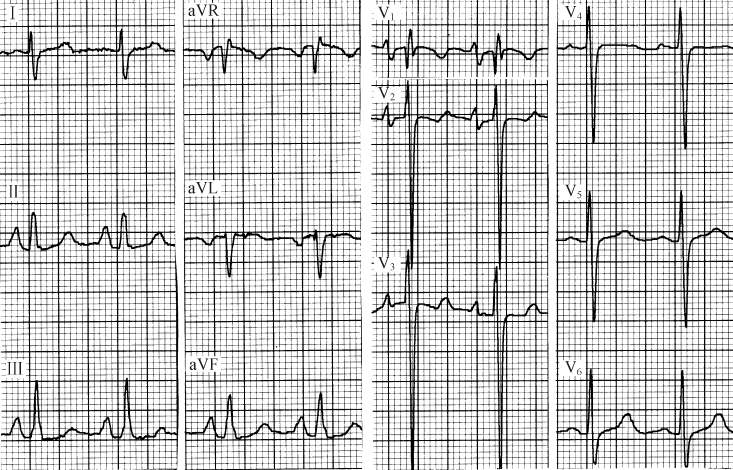
\includegraphics[width=3.36458in,height=2in]{./images/Image00008.jpg}
\end{table}

周围型位置性眩晕、眼震的常见疾病有良性阵发性位置性眩晕(即耳石病)、梅尼埃病、耳硬化症、内耳开窗术后、浆液性迷路炎、内听动脉供血不足、药物性内耳损害等。中枢性位置性眩晕、眼震的常见疾病可见于小脑蚓部肿瘤、第四脑室肿瘤或囊肿、椎-基底动脉供血不足、桥小脑角肿瘤、颅脑外伤等。

\paragraph{直流电试验}

应用直流电检查前庭神经,电流不仅刺激前庭末梢器,也能直接作用于前庭神经节及前庭神经。方法为将直流电负极置于测试耳的耳屏处或乳突处,正极置于前额或手中,电流逐渐缓慢增加,分别观察出现眩晕感、倾倒及眼震的毫安(mA)数,通常于正常人2~4mA即有眩晕感觉,4~6mA出现倾倒反应,6~8mA出现眼震。眼震之快相向负极侧,而倾倒则向负极之对侧。直流电试验主要的临床价值可协助鉴别前庭末梢器和前庭神经本身的病变。例如前庭末梢器病变(梅尼埃病、迷路炎)变温试验可能显示病侧前庭功能减退或功能消失,而直流电试验仍属正常反应。若病变累及前庭神经例如听神经瘤,则变温试验无反应时,直流电试验亦无反应。

\paragraph{视动性眼震试验(optokinetic test)}

视动性眼震由固视连续移动景物所引起而非前庭刺激所引起。试验原理:当两眼注视眼前连续而迅速通过的一系列物体时,每一物体在后一物体出现于视野中以前,受到两眼的注视与跟随。而当下一物体的影像落于视网膜的周边部时,眼球即反射性反跳,以便使后一物体像落于黄斑上。眼球如此快慢交替地运动,遂形成视动性眼球震颤,这是一种生理现象。此项检查之所以列入神经耳科学,是因为:①视动性眼震亦有快相与慢相的交替运动,与前庭性眼震形式类似;②此项检查对各种自发性眼震鉴别及颅内病变的定位诊断有一定价值。应用视鼓或视伞或带尺诱发眼球震颤。正常人所诱发之视动性眼震之慢相与视鼓旋转之方向一致,眼震之快相与视鼓旋转之方向相反,所诱发出之视动性眼震向左、右侧是对称的。

一般认为视动性眼球震颤的神经通路为:起自视网膜右半侧之神经纤维→右侧膝状体→视放射→视皮质(Brodman18区、角回和缘上回)的视动中枢,再自视动中枢通过视放射后部深处前行,离视放射→大脑脚→上丘→经内侧纵束→脑桥眼球同向运动中枢→眼球运动核。

因此,皮质视动中枢至脑桥同向运动中枢间任何部位之病变累及视动通路,即可消除或减弱向对侧之视动性眼球震颤,亦即出现向病侧之视动性眼震优势偏向。根据笔者研究的资料分析,在大脑半球占位性病变中,出现视动性眼震优势偏向现象多数与后颞、顶枕部(尤其是顶部)有关。如果病变累及脑干内的视动反射纤维,亦常有异常反应,多数为不对称性异常。在眼源性的自发性眼球震颤病例中,视动性眼震反应多数表现为同向性异常(即眼震的快相与视鼓或视伞旋转的方向相同),或无反应。

\paragraph{眼震电图(ENG)}

检查对于眩晕患者作前庭功能检查,其中自发性眼球震颤与诱发性眼球震颤都是检查中的一项重要体征,除肉眼观察外,应用眼震电图记录,可以使眼球震颤的各种特征(速度、频率、幅度、方向)客观记录下来,以供比较分析研究。通常所见到的节律型、水平性(或垂直性)眼震在眼震电图上表现为一不对称的峰形波,由迅速上升(或下降)的快相与缓慢回复至基线的慢相所组成。

眼震强度可用眼震时程、幅度、频率、慢相速度等表示,其中以时程和慢相速度为可靠。

慢相速度的测量方法如下:①正常眼震电图测量法:见图\ref{fig3-1}。②眼震强度------慢相速度计算法:其中几何作图法(图\ref{fig3-2})系延长慢相斜边成AC,使BC等于纸速1秒(s),若测得AB
= 22mm,定标值10°=
11mm,按速度=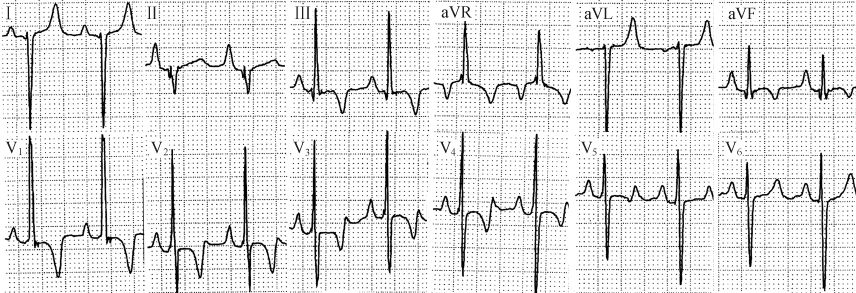
\includegraphics[width=0.30208in,height=0.32292in]{./images/Image00009.jpg}
,得

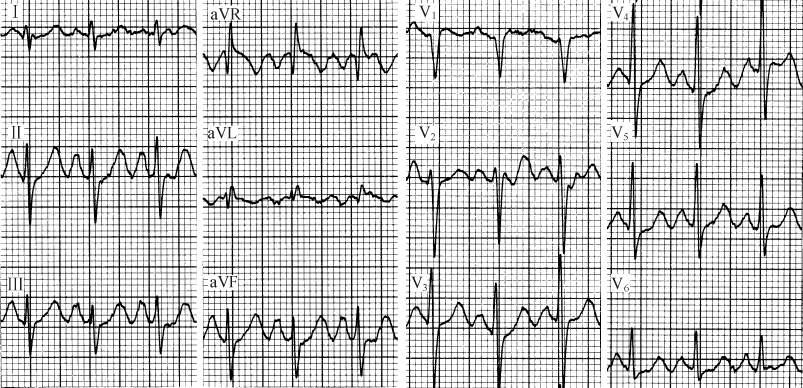
\includegraphics[width=1.95833in,height=0.42708in]{./images/Image00010.jpg}

\begin{figure}[!htbp]
 \centering
 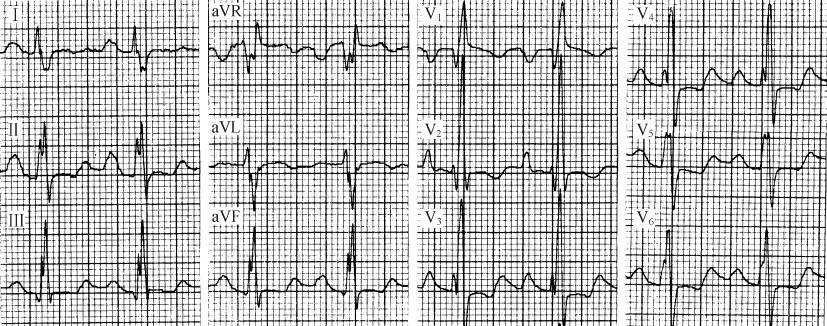
\includegraphics[width=2.75in,height=1.13542in]{./images/Image00011.jpg}
 \captionsetup{justification=centering}
 \caption{正常眼震电图}
 \label{fig3-1}
  \end{figure} 

a.右向眼震;b.左向眼震;c.快相;d.慢相

\begin{figure}[!htbp]
 \centering
 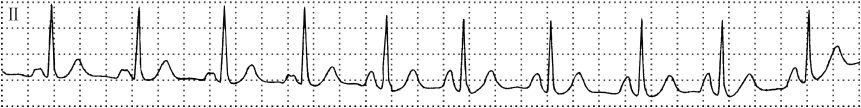
\includegraphics[width=1.96875in,height=1.29167in]{./images/Image00012.jpg}
 \captionsetup{justification=centering}
 \caption{几何作图法}
 \label{fig3-2}
  \end{figure} 

另为极盛期价值法(culmination
valve),于变温试验中,取反应高潮期10秒内之眼震,计算其幅度和频率,以慢相速度表示之。其公式如下:

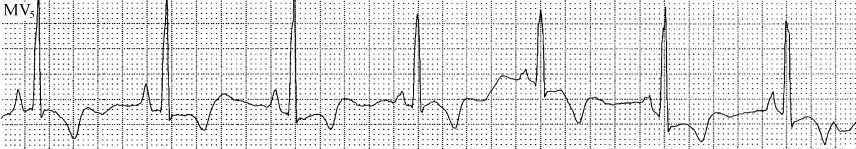
\includegraphics[width=2.16667in,height=0.53125in]{./images/Image00013.jpg}

例如:10秒内眼震总幅为150mm,总次数为20次,定标值10°= 11mm,则

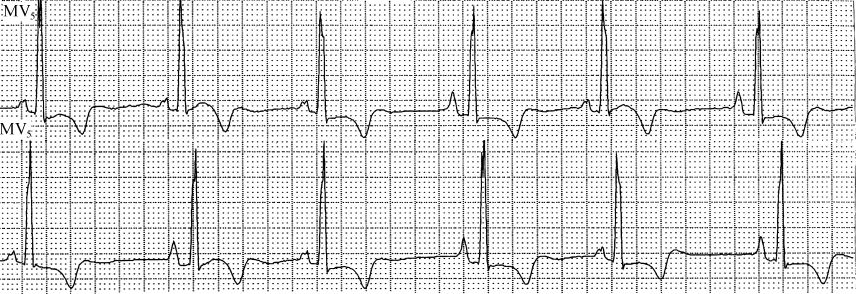
\includegraphics[width=2.57292in,height=0.40625in]{./images/Image00014.jpg}

利用眼震电图可以记录各种自发性眼震,并通过各种诱发试验记录变温性、位置性、视动性、凝视性眼球震颤。并可作扫视试验(saccade
test)、平稳跟踪试验(pursuit
test),于检查中可进一步观察在睁眼(明亮条件下)、暗室中、闭眼条件下眼震的变化。这些客观资料,均有助于对眩晕、眼震、前庭系统疾病的诊断。

\subsubsection{诊断注意事项}

对于临床医师而言,在对眩晕的病因作诊断与鉴别诊断时可先从以下几方面考虑:

1.前庭系统性眩晕抑或非系统性眩晕
一般而言,凡属前庭系统性眩晕均具有空间定向的感觉异常,具有运动错觉或运动幻觉的特点,或觉外境或觉自身在运动感(旋转、摇晃、向一侧移动);而非系统性眩晕则没有上述的特点,大多数患者对“眩晕”描述为头昏、头胀、头重脚轻、头脑内转动等。

2.前庭周围性眩晕抑或前庭中枢性眩晕
对于前庭系统性眩晕应进一步鉴别是前庭周围性病变还是前庭中枢性病变,两者的鉴别见表\ref{tab3-2}。

\begin{table}[htbp]
\centering
\caption{前庭周围性眩晕与前庭中枢性眩晕的鉴别}
\label{tab3-2}
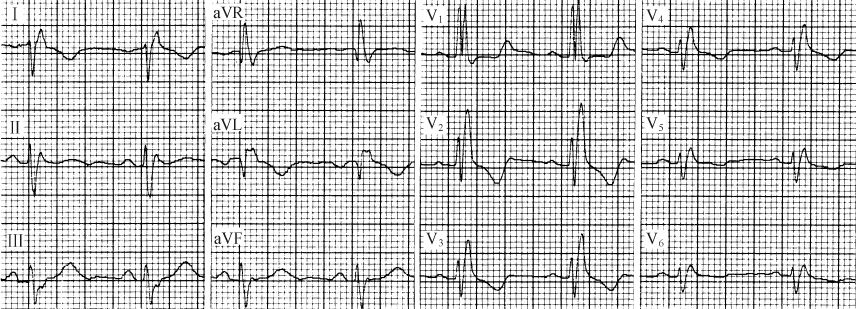
\includegraphics[width=3.3125in,height=2.78125in]{./images/Image00015.jpg}
\end{table}

3.更进一步的诊断需根据各疾病的临床表现的特点及必要的辅助检查。

\subsubsection{常见眩晕症疾患的临床特点}

\hypertarget{text00012.htmlux5cux23CHP1-3-2-6-1}{}
(一) 梅尼埃病(Ménière disease)

梅尼埃病系内耳病变,为中年以上阵发性眩晕的最常见的原因。临床表现为典型的三联症状:发作性眩晕,波动性、渐进性、感音性的听力减退和耳鸣。眩晕发作时常伴有恶心、呕吐、出汗、面色苍白、眼球震颤。眩晕常突然发作,发作前耳鸣增加,听力骤减,耳内有饱胀感。每次眩晕发作历时数小时至数天(多系1~2天)而自行缓解。发作间歇期长短不一,多数为数月一次,亦有一个月数次者。眩晕发作常常随耳聋的进展而减少,至完全耳聋时,迷路前庭功能消失,眩晕发作亦常终止。于眩晕发作间歇期间检查,仅可发现单侧(少数为双侧)感音性耳聋,作电测听检查部分患者重振试验(recruitment
test)呈阳性。前庭功能变温试验于一部分病例中显示功能减退。本病产生的原因可能是支配前庭器的交感神经功能失调引起迷路动脉痉挛,从而使内淋巴产生过多或吸收障碍,导致迷路水肿及内淋巴系压力增高,内淋巴腔扩大及内耳末梢器缺氧、变性等病理变化。

\hypertarget{text00012.htmlux5cux23CHP1-3-2-6-2}{}
(二) 良性发作性位置性眩晕(benign paroxysmal positional
vertigo,BPPV)

本病多见于中年以上患者,多数学者认为是耳石器病变所致,故又称此病为耳石病。患者常诉说当头部处于某一位置时即引起头晕,有些患者诉说半夜翻身时突然发生眩晕,若再回复该头位又即会再发生,因而患者尽可能回避该头位。眩晕严重时伴有恶心、呕吐。常无听力障碍。作头位位置检查,常能在患者所诉说的那个头位引起眩晕,同时可见有短暂的水平兼旋转性眼球震颤,眩晕与眼震一致,持续10~20秒自行缓解。重复该头位可重复出现眩晕与眼震。但于短期内连续数次重复检查,则可逐步适应而不出现眩晕症状与眼震。变温试验提示前庭功能正常。病程常为自限性,数周至几个月后可自愈。近年来一些学者研究认为其基本病理机制系椭圆囊斑上耳石脱落、游离的耳石进入后半规管并在内淋巴内移动,在头位变动时刺激后壶腹嵴,于是乃产生短时间的眩晕。至于耳石器病变的原因主要有:①前庭动脉前支血栓形成;②颅脑外伤致内耳震荡。在作头位位置试验时,重复数次检查后之所以出现适应(疲劳)现象是由于耳石散落在内淋巴腔,一时未能沉积在后壶腹顶部,故不再引起症状,但待耳石沉积在壶腹顶部时可再度诱发位置性眩晕与眼震。

\hypertarget{text00012.htmlux5cux23CHP1-3-2-6-3}{}
(三) 非良性位置性眩晕

颅后窝的占位性病变也可引起位置性眩晕
,这与上述良性位置性眩晕在临床表现上有以下区别:此种眩晕的发生往往在头位改变后立即出现,无潜伏期,诱发之眩晕持续时间较长,往往引起恶心、呕吐,眩晕可在数种头位诱发,而不像BPPV只在较特定的1~2种头位才诱发。常见的疾病是第四脑室、小脑蚓部的肿瘤或第四脑室的囊肿,亦可见于小脑半球、脑桥小脑角的肿瘤。除位置性眩晕外,有时有肢体或躯干的共济失调。

\hypertarget{text00012.htmlux5cux23CHP1-3-2-6-4}{}
(四) 前庭神经元炎(vestibular neuronitis)

起病较急,表现为突起的剧烈的眩晕,伴有恶心、呕吐,但无耳蜗症状。起病时常伴有感染(多为上呼吸道)症状,可能是一种病毒感染。发病时有自发性水平性眼球震颤,躯体平衡失调。变温试验显示病侧前庭功能减退或缺失,有时双侧均有损害。预后良好,一般在数周后眩晕症状逐日减轻,但变温试验示前庭功能呈永久性损害。多数学者认为病变主要为病毒侵犯前庭神经的Scarpa神经节,但也有少数学者认为有时脑干内的前庭纤维也受侵犯。

\hypertarget{text00012.htmlux5cux23CHP1-3-2-6-5}{}
(五) 迷路炎

单纯性中耳炎由于炎症刺激使迷路充血可引起眩晕。眩晕程度较轻,中耳炎好转后眩晕亦即解除。中耳炎并发弥漫性化脓性迷路炎时,眩晕严重,伴恶心、呕吐、眼震及病侧听力严重丧失,病侧前庭功能消失。此外还有耳痛、耳漏、头痛、发热等中耳感染症状与体征。慢性中耳炎侵蚀骨迷路有瘘管形成时,常有反复发作的眩晕。瘘管试验(以希格尔镜利用橡皮球增减外耳道压力,通过瘘管影响迷路,产生前庭反应)呈阳性反应。提示内耳有瘘管存在。

\hypertarget{text00012.htmlux5cux23CHP1-3-2-6-6}{}
(六) 药物性眩晕

在临床药物应用中
,有些药物因使用不当,因毒性作用而致眩晕,如链霉素;有些是难以避免的副作用,如某些镇静药和安眠药;有些是过敏所引起。

\paragraph{耳毒性抗生素类}

以氨基糖苷类为主,如链霉素(尤其是硫酸链霉素)、新霉素、卡那霉素、庆大霉素、阿米卡星(丁胺卡那霉素)等,其他尚有万古霉素、多黏菌素B。其中有些药物性损害主要影响前庭部分,但大多数前庭与耳蜗均有影响。链霉素是最常见者,引起眩晕症状通常于疗程第4周出现,但亦有仅应用4天即有眩晕症状者。在年老患者或有肾功能不全的患者,更易出现毒性作用。眩晕症状持续,而在患者行走、头部转动或转身时症状更为明显。于静止时、头部不动时,上述症状明显好转,甚至消失。而一旦活动后上述症状又复出现。前庭功能检查,大多数患者均无自发性眼球震颤,闭目难立征阳性,向左右前后摇晃方向不定。变温试验示双侧前庭功能均明显减退或消失。如伴有耳蜗损害,则尚有双侧感音性耳聋。眩晕症状消失较为缓慢,需数月甚或1~2年之久,前庭功能则更难恢复。

\paragraph{麻醉 、镇静和催眠药}

这类药物引起眩晕的机制主要是对中枢的抑制作用,皮质中枢受抑制时表现为头晕及轻度失平衡,并无明确的运动错觉。于麻醉后,由于皮质中枢的强抑制,有关平衡的各种传入信息,不能在中枢获得综合与分析,因而出现头晕症状,患者诉说昏昏沉沉。这些药物中除麻醉药外还有异丙嗪(非那更)、苯巴比妥(鲁米那)、利眠宁(氯氮{}
)等。

\paragraph{抗癫痫药}

在抗癫痫药中苯妥英钠与扑米酮是引起眩晕的最常见者,尤其是苯妥英钠,因应用广,应用时间又长,如不注意服用剂量及检测药物血药浓度,则甚易引起中毒性损害。主要损害于前庭末梢器,可累及小脑,均可导致眩晕,平衡失调,眼球震颤,共济失调,因此对于这些患者应定期随访,必要时检测药物血药浓度,调整药物剂量。扑米酮能用于抗痫治疗,虽较少用,但初服此药时,其剂量应减少至甚小量(成人常规用量之1/3~1/4),然后缓慢增加,才可避免眩晕。

\paragraph{其他药物}

如水杨酸类(水杨酸钠)、噻嗪类利尿剂(氢氯噻嗪)、降压药(利血平、降压灵)及某些磺胺类药均可致眩晕,在临床应用时应予注意。

\hypertarget{text00012.htmlux5cux23CHP1-3-2-6-7}{}
(七) 血管性眩晕(椎-基底动脉血循环障碍)

\paragraph{迷路卒中}

由于动脉粥样硬化或伴有血液黏稠度增加,血压的偏低,导致内听动脉血栓形成,常产生急骤的、严重的眩晕,伴恶心、呕吐,若耳蜗分支同时受损,则伴有耳聋及耳鸣。患者年龄较大,起病甚快,有身体其他部位动脉硬化的征象,既往(青、中年时)无类似的眩晕发作史等特点,均有助于与其他急性眩晕相鉴别。但有的患者表现短暂性的眩晕发作,伴有或不伴有耳蜗症状,持续数分钟至数小时即缓解,对于这些中、老年患者,若除外耳源性眩晕的其他疾病,可诊断为迷路动脉短暂性缺血发作(TIA)。

\paragraph{小脑后下动脉血栓形成}

亦称延髓外侧综合征(Wallenberg
syndrome)。其典型的症状与体征包括突起眩晕,伴恶心、呕吐,眼球震颤;病侧肢体共济失调及颈交感神经麻痹综合征;吞咽困难及同侧软腭麻痹、声带麻痹;病侧面部及对侧躯体、肢体的痛温觉减退或消失。

\paragraph{椎-基底动脉供血不足(vertebrobasilar insufficiency,VBI)}

多数表现为椎-基底动脉的TIA,临床常见。有关本病的概念至今还不十分清楚。引起VBI的病例基础是:①椎动脉的解剖特点:起始于两侧锁骨下动脉之椎动脉,需穿过第6~1颈椎横突孔后再经枕大孔入路,然后合并为基底动脉,椎动脉在行程中需经过一条活动度较大的骨性隧道。②椎动脉易发生动脉粥样硬化,随着年龄增大其动脉管径逐渐变窄,血流量亦渐变少。③中年以后颈椎常发生退行性变及骨赘形成。因此椎动脉的血流易受到各种因素的影响,例如颈部的转动,血压的较快的降低,血管的痉挛,血黏度的增高。因此VBI的发病通常认为主要是动力学改变所致,但也有部分患者VBI是由于循环系统内的微栓子所造成。由于迷路、前庭神经核、小脑的血液供应均来源于椎-基底动脉血流循环,因此VBI的主要临床表现是眩晕,常突然发生,颈部过度伸屈或旋转有时可诱发,眩晕发作持续通常短暂,常常数分钟即缓解,但可在短时期内反复发生多次,眩晕发作时可伴有恶心、呕吐、站立不稳,亦可伴有椎-基底动脉的其他供应区缺血的临床征象,例如视幻觉、偏盲、猝倒发作、复视、面麻木、进食吞咽困难,肢体肌力减退或感觉障碍,共济失调。上述这些临床表现通常都是呈发作性、短暂性,症状持续数分钟至数小时,不超过24小时,这一类型的VBI可称之为VBTIA(椎-基底动脉短暂性缺血性发作),但临床上也有一部分患者表现为在一段时期内(数天至数周)经常性的头晕,行走不稳,在除外了其他引起眩晕的疾病后亦应考虑为VBI,推究其发病机制是后循环的动力学障碍所致,应予重视。

对于VBI的诊断应根据具体情况选择作下列检查:①颈椎X线片,包括正、侧及斜位片,以发现有无颈椎病及其严重程度及了解有无骨刺可能累及椎动脉。②颈椎CT或颈椎MRI或螺旋CT,以进一步了解颈椎骨骼及脊髓和有关椎动脉受压、变窄情况。③头颅MRA,以了解颅内血管情况,尤其是了解椎-基底动脉及颅内脑底动脉环情况。④TCD检查。⑤BAEP检查。⑥SPECT检查。上述三项检查在VBI的病例中均有相当的阳性率,可作为诊断的参考依据。⑦前庭功能检查主要是作变温试验,对于了解前庭功能有肯定的价值。⑧眼震电图检查:可作扫视试验、凝视试验、跟踪试验、视动试验。有一定的临床价值。

关于椎-基底动脉短暂性缺血性发作的诊断依据:①中老年患者(发病在50岁以上)。②发作性眩晕,每次持续时间短暂,通常为数分钟至数十分钟。③眩晕发作时可伴有一种或数种脑干、小脑、枕叶的缺血症状及体征。④临床症状除轻度眩晕,行走不稳外均在24小时内减轻以至消失。⑤实验室检查(上已述及)有两项以上的阳性发现。⑥排除引起眩晕的其他病因。

\paragraph{颈椎病变}

颈椎退行性病变导致椎间隙狭窄,及由于钩椎关节骨赘增生刺激或压迫椎动脉,使椎动脉痉挛、阻塞,当转颈时一侧之椎动脉更易受压。若椎动脉本身已有粥样硬化,一侧椎动脉受压后,对侧椎动脉无法代偿则出现症状。临床常见之症状为发作性眩晕,其发病与头颈转动有密切关系。此外,这些患者尚可伴有枕部头痛、猝倒、视觉症状(闪光、视野缺失)及上肢麻痛。颈椎X线片、颈CT扫描可显示颈椎形态学病变改变。

\hypertarget{text00012.htmlux5cux23CHP1-3-2-6-8}{}
(八) 颅内肿瘤

由于颅内肿瘤所产生的眩晕有两种机制
:一是由于肿瘤直接压迫、浸润前庭神经或其中枢连接;另一是由于颅内压增高,尤其是由于肿瘤阻塞脑脊液循环而产生脑积水,引起第四脑室底部前庭核的充血和水肿。

\paragraph{桥小脑角肿瘤}

特别是听神经瘤,有轻度眩晕和耳鸣、耳聋,这是听神经瘤的早期症状。病变进一步发展可出现邻近脑神经受损的体征,如病侧角膜反射减退、面部麻木及感觉减退,展神经麻痹、周围性面瘫、眼球震颤,同侧肢体共济失调。在听神经瘤的早期通常并没有自发性眼球震颤,当肿瘤增大压迫脑干或小脑时才会出现,但一经出现则持续存在。听神经瘤至病程后期还可出现颅内压增高症状,头痛、视神经乳头水肿。对于听神经瘤的早期诊断可根据单侧性听力渐进性减退、听力检查为感音性耳聋;同侧前庭功能早期即消失,邻近脑神经(三叉、展、面神经)中有一根受累即应考虑为听神经瘤。若脑脊液中蛋白质含量增加,X线片上示病侧内听道扩大诊断即可肯定。近年来由于应用头颅CT及MRI检查,更易得到早期确诊。

\paragraph{脑干}

(延髓脑桥)肿瘤
因病变累及前庭神经核,常有眩晕及持久的眼震,可有一侧或双侧听力减退,水平性眼震的方向通常为双向性,向左侧注视时快相向左,向右侧注视则快相向右,也可能兼有旋转性眼震。当眼震明显时,眩晕症状不一定很重。还可以有其他脑神经障碍(主要为第Ⅴ、Ⅵ、Ⅶ、Ⅹ、Ⅺ)及对侧肢体瘫痪。

\paragraph{小脑半球肿瘤}

常有眩晕,早期即出现明显的振幅粗大的眼球震颤,及病侧肢体共济失调,水平性眼震的方向通常是两侧性的,但主要是向病变一侧。前庭功能变温试验示病侧肢体偏斜反应不明显。

\paragraph{小脑蚓部肿瘤及第四脑室肿瘤(或囊肿)}

眩晕为常见症状,眩晕的发生或加重常与头位位置有关。作头部位置试验,可见有中枢型位置性眼球震颤,并有早期颅内压增高及固定头位等临床表现。

\paragraph{天幕上肿瘤}

通常并不出现眩晕,如有则可能与颅内压力增高有关,但颞叶肿瘤有时可出现以眩晕为主要表现的癫痫样发作。脑电图上可以有痫样发放。

\hypertarget{text00012.htmlux5cux23CHP1-3-2-6-9}{}
(九) 外伤性眩晕

颅脑外伤时可因内耳迷路
、第Ⅷ脑神经、中枢前庭核及其中枢连接受损而产生眩晕。这些结构可单独或合并受损。迷路内外伤性出血的患者有周围型的前庭紊乱症状,常有颞骨骨折及听力同时受损的征象。亦有内耳并无出血而为迷路震荡者,则眩晕症状持续时间短、恢复较快,听力障碍程度亦较轻。部分患者可由于耳石器损伤而出现短期的位置性眩晕。颞骨横行骨折,骨折线横断岩锥,可产生听神经直接受损,出现明显的眩晕、自发性眼震、听力丧失,于4~6周内前庭症状逐渐消失,但听力常难以恢复。

严重的颅脑损伤患者,在第四脑室及导水管周围可见有点状的少量出血,损伤涉及前庭核及其中枢连接。脑干损伤后产生眩晕的同时常伴有脑干损伤的其他体征,如复视、面瘫、瞳孔不等大、肢体运动或感觉障碍等。眩晕症状持续较久,可达数月以上。颈部鞭索样损伤后亦常有眩晕症状,在头部运动时,尤其是向着颈部鞭索样受损的方向运动时,眩晕症状更易出现。每次眩晕发作数秒至数分钟。头位位置试验可有位置性眼震,常发生于头部转向鞭索样损伤侧,可能是由于内耳耳石器受损所致。

\hypertarget{text00012.htmlux5cux23CHP1-3-2-6-10}{}
(十) 精神性眩晕

精神性眩晕在本质上是神经症的一种表现。大多感觉头昏脑胀,非真性眩晕,无运动错觉,患者诉“眩晕”、“头晕”时无自发性眼震或自发性倾倒,往往常有神经症其他表现如失眠、焦虑、紧张、记忆力减退、注意力难集中等。无前庭系或非前庭系器官性疾病。起病诱因系以情绪、精神因素为主。

\subsection{处理原则}

\subsubsection{一般处理}

对于急性眩晕发作的患者,需卧床休息,饮食以流质为宜。伴有明显恶心、呕吐者,应酌情给予静脉补液,以维持营养,并需注意水、电解质的平衡。对于焦虑紧张的患者,应给予适当的病情解释与安慰,以解除顾虑。眩晕发作缓解后,应鼓励患者早日逐渐参加日常活动,适应日常生活。

\subsubsection{病因治疗}

因中耳炎并发症引起的急性化脓性迷路炎,应由耳科作必要的手术及抗感染治疗。由颅内占位性病变如小脑肿瘤、听神经瘤引起者,需作手术摘除肿瘤。由于梅尼埃病产生的眩晕,主张调节自主神经功能,平时以低盐饮食为宜。对于由药物中毒性损害引起的眩晕患者,应及时停药,并给予维生素B族药物。因颈椎骨质增生、椎间盘膨隆或突出而致的眩晕,可先作颈椎牵引或作颈托固定。必要时再考虑手术治疗。因心律失常或血压过高、偏低者,则需给予相应的内科治疗。因贫血引起的眩晕应纠正贫血。凡此种种的有关病因的处理均属重要,不可忽视。

\subsubsection{对症处理}

在病因治疗的同时,对于眩晕症状需给予药物治疗,以减轻眩晕症状及减少伴发的恶心、呕吐、焦虑、紧张等症状。

\paragraph{急性发作期的药物治疗}

可考虑选用的药物有:氢溴酸东莨菪碱0.3mg,肌肉注射;茶苯海明(晕海宁,dramamine)50mg,肌肉注射;硫酸阿托品0.5~1mg,肌肉注射;山莨菪碱(654-2)5~10mg,肌肉注射;盐酸异丙嗪(非那更)25~50mg,肌肉注射。以上药物可选择应用,并可根据病情每隔4~6小时重复给药2~3次。

\paragraph{眩晕发作后尚有轻度症状或慢性眩晕的治疗}

在急性眩晕发作后,虽已无明显的旋转幻觉,但仍有平衡失调、站立不稳的感觉,或在头部、身体转动时有这些症状,或眩晕程度虽轻但经常存在者,可选用各种镇静剂、安定剂,例如苯巴比妥0.015~0.03g,或地西泮(安定)2.5~5mg,或氯丙嗪25mg等,均为每天2~3次,口服。

\paragraph{几种治疗眩晕症的常用药物}

\hypertarget{text00012.htmlux5cux23CHP1-3-3-3-3-1}{}
(1) 镇静剂与安定剂:

例如苯巴比妥、溴剂、地西泮等。它们的药理作用对于前庭反应有抑制作用,对于一般感觉亦起抑制作用,因此可以减轻眩晕症状,消除紧张、烦躁不安、焦虑等症状。苯巴比妥虽可以减轻眩晕,但也常有全身抑制的作用,如疲倦、乏力。地西泮能减轻眩晕症状,减少紧张、焦虑,并有止吐作用,但可加强其他中枢抑制剂的作用。大剂量的安定类药物可以引起锥体外系的副作用。

\hypertarget{text00012.htmlux5cux23CHP1-3-3-3-3-2}{}
(2) 抗组胺药物:

例如苯海拉明、盐酸异丙嗪、氯苯那敏、盐酸氯苯苄嗪(敏克静)、茶苯海明等,这些药物用于治疗眩晕,其治疗效应可能是由于它们药理上的镇静作用而不是抗组胺作用。它们应用于眩晕发作期尚有止吐作用。

\hypertarget{text00012.htmlux5cux23CHP1-3-3-3-3-3}{}
(3) 止吐剂:

常用者为盐酸氯苯苄嗪及异丙嗪,均有明显止吐作用,适用于运动病及眩晕时伴有明显的自主神经反应(恶心、呕吐)的病例。这些药物亦有镇静作用及抗组胺作用。

\hypertarget{text00012.htmlux5cux23CHP1-3-3-3-3-4}{}
(4) 抗胆碱药物:

常用药物系东莨菪碱与阿托品,对于梅尼埃病的治疗效果较好。这类药物尚有止吐及解除血管痉挛的作用。东莨菪碱还有镇静作用,可优选使用。

\hypertarget{text00012.htmlux5cux23CHP1-3-3-3-3-5}{}
(5) 血管舒张药物:

例如烟酸、妥拉唑啉、山莨菪碱、地巴唑,这些药物并不是前庭抑制药物,其药理作用为解除血管痉挛。可应用于因血管痉挛、缺血性病变所引起的眩晕,如梅尼埃病的发作期及椎-基底动脉供血不足的病例。此外倍他司汀(betahistine,抗眩啶)亦有扩张血管的作用,常用量为4mg,每日3次;甲磺酸倍他司汀(敏斯朗)亦有类似的作用,6mg,每日3次口服。

\hypertarget{text00012.htmlux5cux23CHP1-3-3-3-3-6}{}
(6) 钙拮抗剂:

目前常用者有尼莫地平20mg,每天3次;桂利嗪(脑益嗪)25mg;每天3次,氟桂利嗪(flunarizine,商品名西比灵)5mg,每天1~2次,均为口服。

\hypertarget{text00012.htmlux5cux23CHP1-3-3-3-3-7}{}
(7) 增强动脉血氧分压和血氧饱和度药物:

阿米三嗪萝巴新{[}都可喜(Duxil){]}内含阿米三嗪和萝巴新,本药可增迷路和脑组织的血氧供应,对于因缺血缺氧而产生的眩晕疾患有较好的疗效,常用量为30mg,每天2次,口服。


\hypertarget{text00013.htmlux5cux23CHP1-3-4}{}
参 考 文 献

1. 史玉泉.实用神经病学.第3版.上海:上海科学技术出版社,2004

2. Norre ME. Clinical value of caloric test. Clin
Otolaryngol,1988,13:247

\protect\hypertarget{text00014.html}{}{}

\chapter{晕 厥}

晕厥(syncope)又称昏厥,是由于短暂的全脑组织灌注降低而导致的一过性意识丧失(transient
loss of
consciousness,TLOC),以快速发作、持续时间短和自限性为特点。可因血管迷走反射、直立性低血压、心输出量减少引起全脑低灌注,或由于脑干椎-基底动脉缺血引起脑干选择性低灌注所致。晕厥发作起病突然,持续时间短,典型可分为三期,其基本临床特点为:①发作前期:患者常感头部及全身不适、头晕、视力模糊、耳鸣、面色苍白、出汗,预示即将发生晕厥;此时患者如取头低位躺卧姿势常可防止发作。②发作期:轻者眩晕、恶心、躯体发软,眼前发黑,重者常突然意识丧失,全身肌紧张度消失,跌倒地上。意识丧失超过15~20秒可发生阵挛动作,有时有呼吸暂停,心率减慢,甚至心脏暂停搏动,瞳孔散大,流涎,尿失禁等;其特点是发作时间短暂,一般持续1~2分钟左右。脑电图检查可见持续3~10秒的广泛性、对称性2~3Hz的慢波。③发作后期(恢复期):患者平卧后意识迅速恢复(数秒至数分钟),可遗留紧张、头晕、头痛、恶心、苍白、出汗、无力和便意感等,甚至呕吐及括约肌失禁。休息数分或数十分钟缓解,不留后遗症,偶有极短暂的(<
30秒)发作后模糊状态伴定向力障碍和易激惹。

可见晕厥的特征是:发作突然,意识丧失时间短,不能维持正常姿势或倒地,在短时间内迅速恢复,罕有后遗症。

当前急诊对晕厥的评估已经从诊断晕厥的病因转变为进行危险分层,其目的是:①识别有威胁生命的疾病并收入院;②识别低危患者,可以让他们离院,并且以后到专科就诊;③识别不需要进一步诊断和治疗的患者;④对初步评估不能得出结论的患者进行进一步检查。

\subsection{病因与发病机制}

引起晕厥的病因很多(表\ref{tab4-1}),但任何原因均是通过影响脑血流,引起脑血供障碍所致。人脑重量占体重的2\%,而脑耗氧量却占全身耗氧量的20\%。脑组织几乎无氧和葡萄糖储备,全靠血循环提供外源性补给才能维持其正常的生理功能。健康成人的脑血流量为每100g脑组织45~50ml/分钟,而维持人的意识水平所需最低限度的脑血流量(即临界值)为每100g脑组织30ml/分钟,当脑血流量骤减至此临界值则可发生晕厥。

\paragraph{反射性晕厥(神经介导的晕厥)}

此类晕厥主要由于在正常状态下控制循环系统的心血管反射对刺激因素出现间歇性的不恰当反应,引起血管扩张和(或)心动过缓,导致动脉血压降低及全脑灌注减少。依据诱发因素不同又可分为以下几类:

\begin{table}[htbp]
\centering
\caption{晕厥的病因分类}
\label{tab4-1}
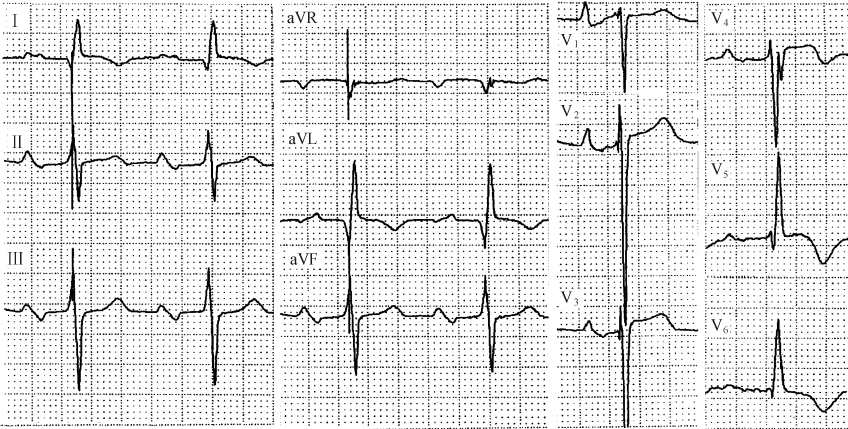
\includegraphics[width=3.30208in,height=7.11458in]{./images/Image00017.jpg}
\end{table}

\hypertarget{text00014.htmlux5cux23CHP1-4-1-1-1}{}
(1) 血管迷走性晕厥:

是最常见的晕厥类型,由情绪或直立位诱发,常伴自主神经激活的前驱症状(大汗、苍白或恶心)。

\hypertarget{text00014.htmlux5cux23CHP1-4-1-1-2}{}
(2) 情境性晕厥:

与一些特殊情境相关,如运动后晕厥等。

\hypertarget{text00014.htmlux5cux23CHP1-4-1-1-3}{}
(3) 颈动脉窦晕厥:

常由非机械性刺激因素诱发,可通过颈动脉窦按摩来确诊。

\hypertarget{text00014.htmlux5cux23CHP1-4-1-1-4}{}
(4) 不典型晕厥:

多数没有明确的诱发因素,诊断主要基于排除其他晕厥的病因(无器质性心脏病)。

\paragraph{直立性低血压和直立性不耐受综合征}

此类晕厥主要包括以下4种类型:

\hypertarget{text00014.htmlux5cux23CHP1-4-1-2-1}{}
(1) 典型的直立性低血压(OH):

站立3分钟内,收缩压下降≥20mmHg和(或)舒张压下降≥10mmHg,见于单纯性自主神经功能衰竭(ANF)、低血容量或其他形式的ANF。

\hypertarget{text00014.htmlux5cux23CHP1-4-1-2-2}{}
(2) 初始性直立性低血压:

站立即刻血压下降>
40mmHg,然后自发、快速地恢复正常,低血压及其症状持续时间较短(<
30秒)。

\hypertarget{text00014.htmlux5cux23CHP1-4-1-2-3}{}
(3) 延迟(进展性)OH:

其在老年人中并不少见,主要与年龄相关的代偿反射受损有关,以直立状态下收缩压进行性缓慢下降为特点,但不伴心动过缓。

\hypertarget{text00014.htmlux5cux23CHP1-4-1-2-4}{}
(4) 体位性直立性心动过速综合征:

部分患者(主要为年轻女性),表现为严重的直立性不能耐受,但没有晕厥,伴随心率明显加快(增加>
30次/分或达到120次/分以上)和血压不稳定,病理生理机制尚不明确。

\paragraph{心源性晕厥}

\hypertarget{text00014.htmlux5cux23CHP1-4-1-3-1}{}
(1) 心律失常性晕厥:

是心源性晕厥的最常见病因。心律失常诱发血流动力学不稳定,导致心输出量及脑血流量严重减少。心律失常类型包括:病窦综合征(窦房结功能受损,产生窦性停搏及窦房阻滞,以及慢-快综合征)和严重的获得性房室传导阻滞(莫氏Ⅱ型、高度及完全性房室传导阻滞),也可见于药物引起的缓慢性或快速性心律失常,如延长QT间期药物引起的尖端扭转性室速。

\hypertarget{text00014.htmlux5cux23CHP1-4-1-3-2}{}
(2) 器质性心脏病:

主要见于左室流出道梗阻性疾病。

\subsection{流行病学}

晕厥在普通人群中常见,首发年龄多为10~30岁,其中女性约47\%、男性约31\%在15岁左右发生晕厥。迷走性晕厥是导致晕厥的最主要原因,心源性晕厥是导致晕厥的第二位原因。医院中的老年患者心源性晕厥发病率较高。在小于40岁的患者中,OH所导致的晕厥较为少见。个别患者的病情较为复杂,在医疗转诊、救治的过程中,一些非晕厥的意识丧失患者常被误诊为晕厥。需注意的是,反射性晕厥是年轻人群中最为常见的导致TLOC的原因;而老年患者通常病情较为复杂,且相关病史也不及年轻人群可靠。

\subsection{诊断思路}

晕厥的诊断目的包括:①找出确切的原因以便进行有效的、针对病理机制的治疗;②识别患者的风险,这种风险常取决于潜在的疾病,而不是晕厥本身的机制。

\subsubsection{初步评估}

详细的病史询问在多数情况下有助于鉴别晕厥与非晕厥,但有时非常困难,应包含以下问题:

(1) 是否为完全性意识丧失(LOC)?

(2) LOC是否为一过性,伴快速起病及短暂持续?

(3) 患者晕厥是否为自发性、完全恢复且不留后遗症?

(4) 患者是否丧失肌张力?

若上述问题的答案均为肯定的,则晕厥可能性极大。若≥1个问题的答案为否定,则应首先排除其他类型的LOC。

对出现TLOC的患者进行初步评估,除了过去提出的详细询问病史、体格检查(包括测量不同体位血压)以及心电图检查外。提出在此基础上,可以适当增加其他的检查以保证诊断准确:①40岁以上患者建议首先进行颈动脉窦按摩。②对于有心脏病病史或怀疑此次晕厥与器质性心脏病或其他心血管疾病有关的患者,建议进行超声心动图检查。③对于怀疑因心律失常而导致晕厥的患者,应给予实时心电监测。④若晕厥与体位变化有关或怀疑反射性晕厥时,则应进行相关检查。如卧立位试验和(或)直立倾斜试验等。⑤仅在怀疑非晕厥原因造成的TLOC的情况下,进行神经科检查或血液检查。

当初步评估后尚无法明确晕厥原因时,要求立即对患者的主要心血管事件及心源性猝死(SCD)的风险进行评估。具体流程如图\ref{fig4-1}所示。

根据最新的SCD防治指南对晕厥进行了危险分层,见表\ref{tab4-2}。\footnote{LVEF:左室射血分数,SCD =心源性猝死,VT =室性心动过速,LBBB=左束支传导阻滞,RBBB =右束支传导阻滞,ARVC=致心律失常性右室心肌病,心衰=心力衰竭,心梗=心肌梗死}

经过初步评估有些晕厥即可明确诊断,其诊断的建议及级别、证据水平见表\ref{tab4-3}。

\begin{table}[htbp]
\centering
\caption{晕厥的危险分层}
\label{tab4-2}
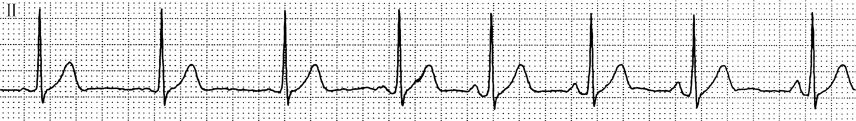
\includegraphics[width=3.28125in,height=4.04167in]{./images/Image00018.jpg}
\end{table}


\begin{figure}[!htbp]
 \centering
 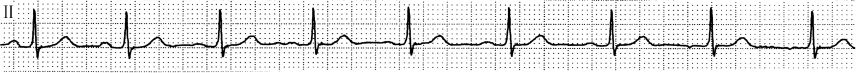
\includegraphics[width=3.84375in,height=3.08333in]{./images/Image00019.jpg}
 \captionsetup{justification=centering}
 \caption{疑似TLOC患者的诊断流程图}
 \label{fig4-1}
  \end{figure} 

\begin{table}[htbp]
\begin{center}
\caption{通过初步评估获得诊断的建议\textsuperscript{*}}
\label{tab4-3}
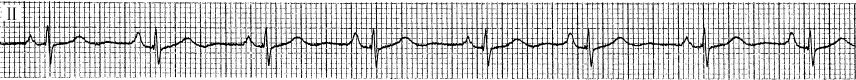
\includegraphics[width=6.66667in,height=2.69792in]{./images/Image00020.jpg}
\end{center}

{\small
*本文的建议均源自2009年ESC晕厥诊断和治疗指南。

建议的级别如下:

Ⅰ级:证据和(或)一致同意给予的诊断操作/处理有益,有用和有效。

Ⅱ级:抵触的证据和(或)关于处理的有用/有效存在分歧的观点。

Ⅱa级:证据/观点偏重于有用/有效。

Ⅱb级:证据/观点偏重于无用/无效。

Ⅲ级:证据或一致同意处理无用/无效,且在某些情况下可能有害。

证据水平如下:

A类证据:数据来自多中心随机临床试验或荟萃分析。

B类证据:数据来自单中心随机临床试验或大的非随机研究。

C类证据:专家的一致观点和(或)小的研究,回顾性研究,注册中心资料。}
\end{table}

\subsubsection{诊断试验}

初步评估后,倾向性诊断需要进一步检查证实,包括心脏评估检查如超声心动图,心脏负荷试验,心电监测包括Holter,必要时埋藏植入式心电事件记录仪(ILR)和电生理检查;神经介导方面的检查包括倾斜试验和颈动脉窦按摩。

\paragraph{颈动脉窦按摩}

压迫颈动脉分叉处能够产生反射性心率减慢和血压下降。某些晕厥患者,特别是>
40岁的患者,可以见到对颈动脉窦按摩的异常反应。室性停搏持续≥3秒,收缩压下降≥50mmHg为异常反应,称为颈动脉窦过敏。颈动脉窦按摩是揭示颈动脉窦过敏综合征晕厥的一种检查方法。2009年ESC晕厥诊断和治疗指南颈动脉窦按摩的适应证和诊断标准见表\ref{tab4-4}。

\begin{table}[htbp]
\centering
\caption{颈动脉窦按摩的适应证和诊断标准}
\label{tab4-4}
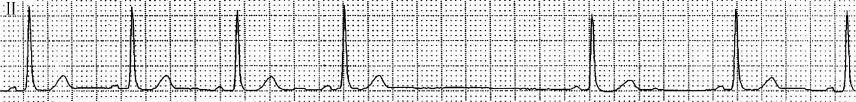
\includegraphics[width=3.34375in,height=1.98958in]{./images/Image00021.jpg}
\end{table}

\paragraph{倾斜试验}

倾斜试验有助于诊断神经介导性晕厥,但是,其敏感性、特异性、诊断标准和重复性存在很大问题,敏感性和特异性与检查方法有密切关系。敏感性26\%~80\%,特异性约90\%。2009年ESC晕厥诊断和治疗指南倾斜试验的适应证和诊断标准见表\ref{tab4-5}。

\paragraph{心电图}

(ECG)监测
ECG监测是诊断间歇性缓慢和快速心律失常的方法,但是ECG监测技术目前仍有严重的局限性。晕厥患者ECG监测的作用不是孤立的。医生可以根据病史、体格检查和其他客观检查如倾斜试验决定治疗方案。有些情况下,临床上强烈提示为反射性晕厥时,无需动态心电图(Holter)监测。如果症状发作不频繁Holter监测对诊断意义也不大,这种情况下应考虑植入式循环记录仪。将来的技术可能会记录ECG以外的多项指标,将把重点放在与自发性晕厥相关的心律方面,而不是被触发的晕厥。了解自发性晕厥发作过程是评估晕厥的最好标准。因此,植入式监测仪对晕厥越来越重要。记录到晕厥时有缓慢心律失常即可考虑诊断,但是,有时需要进一步检查明确是心脏本身原因所致还是神经反射机制造成,而反射性心动过缓可能是阵发性心动过缓最常见的原因。

由于晕厥发作时ILR记录到的心律失常的变异和干扰很大,2009年ESC晕厥诊断和治疗指南采用国际不明原因晕厥研究调查组织(ISSUE)的方法,将心电图记录进行了分类,根据主要心律失常和可能的晕厥机制将心电图划分为4型。

1型:心脏停搏,RR间期≥3秒。1型又分为A、B、C
3个亚型。1A型:窦性停搏,表现为进行性窦性心动过缓或初为窦性心动过速逐渐进展为窦性心动过缓直至发生窦性停搏,其可能的机制为反射性。1B型:窦性心动过缓合并房室传导阻滞,表现为进行性窦性心动过缓随后出现房室传导阻滞(和心室停搏)的同时伴有窦率下降;或突发房室传导阻滞(和心室停搏)伴窦率下降,其可能机制为反射性。1C型:房室传导阻滞,突发房室传导阻滞(和心室停搏)伴窦律逐渐增加,其可能机制为自身病变。

2型:心动过缓,心率下降> 30\%或心率<
40次/分持续超过10秒,其可能机制为反射性。

3型:无或很小的心率变异性,心率变异度< 30\%且心率>
40次/分,其机制不肯定。

4型:心动过速,心率增加> 30\%,心率> 120次/分。此型又分为A、B、C、D
4型。4A型:进行性窦性心动过速,机制不肯定。4B型:心房颤动(简称房颤)。4C型:SVT(不包括窦性)。4D型:VT。

\begin{table}[htbp]
\centering
\caption{倾斜试验的适应证和诊断标准}
\label{tab4-5}
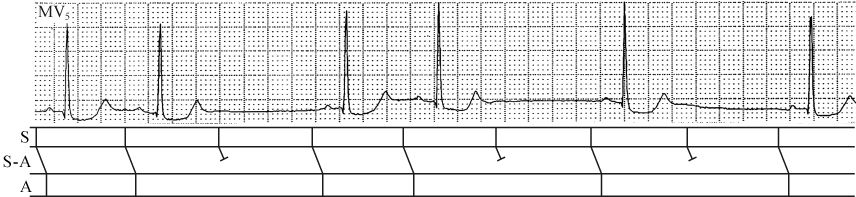
\includegraphics[width=3.21875in,height=6.40625in]{./images/Image00022.jpg}
\end{table}

2009年 ESC晕厥诊断和治疗指南心电图监测的建议见表\ref{tab4-6}。

\paragraph{电生理检查}

电生理检查通过心内膜和心外膜(冠状窦电极)刺激并记录揭示引起晕厥的原发性心律失常的心电异常改变。然而,仅有少数研究应用Holter和植入式记录仪证实了电生理检查的结果。电生理检查揭示的真实诊断仅仅涵盖了一部分患者。下列诊断标准广泛用于确定窦房结功能障碍:窦房结恢复时间(SNRT)>
1.6秒或2秒或校正的窦房结恢复时间(CSNRT)> 525毫秒。另一项研究认为SNRT
>
3秒诊断窦房结功能障碍性晕厥的可能性更大。2009年ESC晕厥诊断和治疗指南电生理检查的适应证见表\ref{tab4-7}。\footnote{ARVC:致心律失常型右室心肌病;HCM:肥厚型心肌病}

\begin{table}[htbp]
\centering
\caption{心电图监测的建议}
\label{tab4-6}
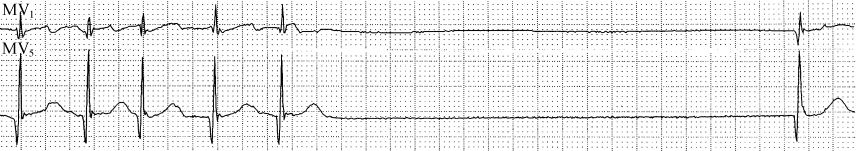
\includegraphics[width=3.25in,height=3.30208in]{./images/Image00023.jpg}
\end{table}

\begin{table}[htbp]
\centering
\caption{电生理检查的适应证}
\label{tab4-7}
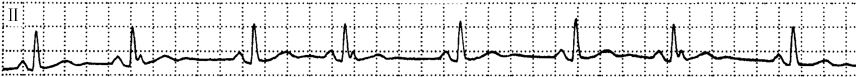
\includegraphics[width=3.25in,height=2.9375in]{./images/Image00024.jpg}
\end{table}



\paragraph{超声心动图(UCG)}

当病史、体格检查和心电图检查不能发现晕厥的原因时,超声心动图检查是发现包括瓣膜病在内的器质性心脏病的有效方法。通过该检查还能发现肺动脉高压和右心室扩大等提示肺栓塞的表现。体格检查正常的晕厥或先兆晕厥患者超声心动图检查最常见的发现是二尖瓣脱垂(4.6\%~18.5\%)。其他心脏异常包括瓣膜病(最常见的是主动脉瓣狭窄)、心肌病、节段性室壁运动异常提示的心肌梗死、冠状动脉畸形、浸润性心脏病如淀粉样变性、心脏肿瘤、动脉瘤、左房血栓等。超声心动图检查为判断晕厥的类型、严重程度及危险分层提供重要的信息。如果发现中重度器质性心脏病应考虑心源性晕厥。另一方面,如果超声心动图仪发现轻微心脏结构病变,则心源性晕厥的可能性较小,应进行非心源性晕厥方面的检查。2009年ESC晕厥诊断和治疗指南UCG适应证和诊断标准见表\ref{tab4-8}。

\begin{table}[htbp]
\centering
\caption{UCG适应证和诊断标准}
\label{tab4-8}
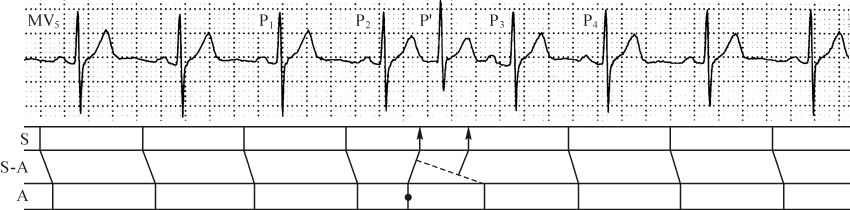
\includegraphics[width=3.20833in,height=1.6875in]{./images/Image00025.jpg}
\end{table}

\paragraph{运动试验}

运动中或运动后即刻发生晕厥的患者应进行运动试验。进行运动试验应该是症状限制性的,即由于运动中和运动后即刻易发生晕厥,运动中和恢复阶段均应监测心电和血压,应做好防范。运动中发生晕厥可能是心脏原因造成的,有些病例报告运动中也可能发生过度反射性血管扩张引起晕厥,反射性晕厥的元凶是低血压而无心动过缓。相反,运动后晕厥几乎都是自主神经功能异常或神经介导机制参与的,其特点是与心动过缓或心脏停搏有关的低血压;一般发生于无心脏病的患者。运动试验用于诊断神经反射性晕厥,其特点是劳力后晕厥。血管迷走神经性晕厥的患者,运动中内脏容量性血管和前臂阻力血管反射性收缩功能障碍。运动试验对一般晕厥患者意义不大,仅有1\%发现异常。尽管如此,对运动性晕厥具有重要诊断价值。2009年ESC晕厥诊断和治疗指南运动试验的适应证和诊断标准见表\ref{tab4-9}。

\begin{table}[htbp]
\centering
\caption{运动试验的适应证和诊断标准}
\label{tab4-9}
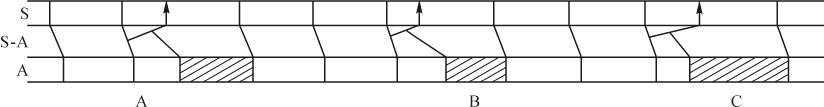
\includegraphics[width=3.25in,height=1.76042in]{./images/Image00026.jpg}
\end{table}

\paragraph{心导管检查}

心导管检查包括评估心腔形态的心室造影、了解冠脉解剖的冠状动脉造影和了解血流、血管内压力和心腔内压力的血流动力学检查。由于是有创检查,一般不作为筛查心源性晕厥的检查。这些检查能够揭示冠状动脉狭窄引起缺血性晕厥:室壁运动异常和心肌收缩力减弱;缺血引起的心律失常、心脏停搏或完全性房室阻滞和缺血诱发的血管迷走神经性反应。也可以揭示冠状动脉痉挛引起的晕厥,这种患者冠状动脉造影中应做麦角新碱试验。

\paragraph{神经系统检查}

神经系统疾病引起的晕厥有三种情况。①自主神经功能障碍:晕厥可以是自主神经系统疾病和功能不全的结果;②有些脑血管疾病也可以引起晕厥(大多是“窃血”综合征);③有些疾病应列为鉴别诊断的内容,因为这些疾病可以引起短暂意识丧失(但不是晕厥,如癫痫)或其发作类似于意识丧失。2009年ESC晕厥诊断和治疗指南神经系统检查适应证见表\ref{tab4-10}。

\begin{table}[htbp]
\centering
\caption{神经系统检查适应证}
\label{tab4-10}
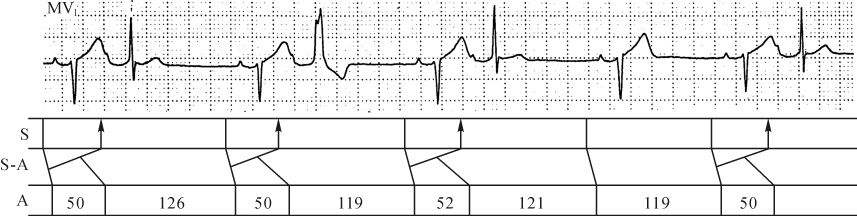
\includegraphics[width=3.25in,height=1.66667in]{./images/Image00027.jpg}
\end{table}

\subsubsection{诊断注意事项}

对所有一过性意识丧失患者必须进行全面仔细的评估,包括病史和检查。要顺序确认:是否晕厥,晕厥的原因,死亡和其他风险。尽管从死亡率角度来说,晕厥常常是良性的,但仅仅确定患者是低死亡风险患者是不够的,因为晕厥常常会复发,增加外伤风险,并且影响生活质量和正常工作。晕厥的诊断和治疗是富于挑战性的。首先,晕厥仅仅是一过性意识丧失众多原因中的一种;其次,患者症状短暂,就诊时一般都已完全恢复,并且有价值的查体发现很少;第三,自发的临床事件很少被医学专业人员目击,临床事件的病史经常是来自“二手”甚至“三手”的资讯。急诊科医生应仔细考虑所发现的异常是否和临床情况相匹配,强调长程监测的重要性。为了使患者得到准确的预后评估和治疗选择,强调应尽可能确定患者的病因。

\subsection{治疗}

\subsubsection{晕厥治疗的一般原则}

晕厥治疗的一般原则是:延长生命、预防复发、防治躯体损伤。

采取基础预防性治疗还是加强治疗取决于下列临床情况:①晕厥的病因。②晕厥复发的可能性大小。③晕厥的死亡危险性大小,主要取决于心脏病和血管病的性质和严重程度。④复发次数或晕厥导致躯体或精神伤害的危险性大小。⑤发生晕厥可能对个人职业或业余爱好造成的影响(如个人经济和生活方式问题)。⑥对公共健康的危险性如汽车司机、飞行员等。⑦对治疗有效性、安全性和不良反应的评估(特别要考虑患者的伴随疾病)。根据晕厥不同病因和机制以及危险分层,采取不同的治疗策略。晕厥的治疗流程见图\ref{fig4-2}。

\paragraph{反射性晕厥的治疗}

反射性晕厥包括血管迷走神经性晕厥、颈动脉窦综合征(CCS)和情景性晕厥,其治疗目标首先是预防症状复发和晕厥相关的损伤,改善生活质量。自2004年指南发表后,治疗方面最大的进展是在生活方式方面上,反射性晕厥非药物治疗的基石是教育,让患者相信这是一种良性情况。一般来讲,最初的治疗涉及让患者了解这一疾病及如何避免诱因(如闷热而拥挤的环境,血容量不足)等相关方面的教育。早期识别前驱症状,采取某些动作以终止发作{[}如仰卧位,身体反压调整(PCMs){]}。避免引起血压降低的药物(包括α受体阻滞剂、利尿剂和酒精)。对于不可预测的频繁发作的晕厥需给予其他治疗。特别是:①非常频繁发作影响到生活质量;②反复晕厥没有或仅有非常短时的晕厥先兆,但患者暴露于有外伤危险的情况下;③晕厥发生在高危作业时(如驾驶、操作机器、飞行、竞技性体育运动等)。

具体治疗方法如下:①身体反压调整(PCMs):非药物的物理治疗,为反射性晕厥的一线治疗。PCMs即双腿肌肉等长收缩PCMs(双腿交叉),或双上肢肌肉等长收缩PCMs(双手紧握和上肢紧绷),多中心前瞻性研究显示,使用这种方法,在反射性晕厥发作时能够显著升高血压,多数情况下可使患者避免或延迟意识丧失。②倾斜训练:可能会减少晕厥复发,但是患者依从性较差,治疗受到影响。③药物治疗:许多试图用于治疗反射性晕厥的药物结果都令人失望。这些药物包括β受体阻滞剂、丙吡胺、东莨菪碱、茶碱、麻黄碱、依替福林、米多君、可乐定和5-羟色胺重吸收抑制剂。由于在反射性晕厥时外周血管常常不能得到适当的收缩,α受体激动血管收缩剂(依替福林和米多君)曾被使用,但是,治疗效果不一致。专家组认为,反射性晕厥患者长期单独使用α受体激动剂药物治疗可能有一些作用,对于偶发患者不建议长期治疗。在长时间站立或从事常常诱发晕厥的活动前1小时服用单剂量的药物避免晕厥发生,对有些患者可能有用。④心脏起搏:起搏治疗反射性晕厥的随机对照试验得出了相反的结果。专家组认为在迷走神经性晕厥中血管减压部分通常起主要作用,所以得出起搏欠佳的结果并不奇怪。而颈动脉窦晕厥心脏起搏治疗可能有效,双腔起搏一般优于单腔心室起搏。反射性晕厥治疗的建议见表\ref{tab4-11}。\footnote{CSS =颈动脉窦综合征;VVS =血管迷走晕厥}

\begin{figure}[!htbp]
 \centering
 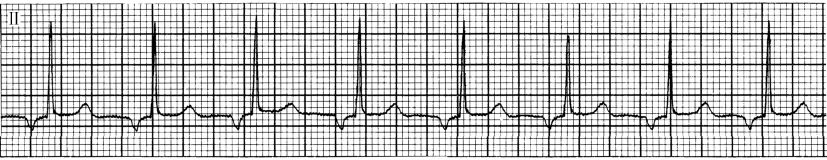
\includegraphics[width=4.82292in,height=2.16667in]{./images/Image00028.jpg}
 \captionsetup{justification=centering}
 \caption{晕厥的治疗流程}
 \label{fig4-2}
  \end{figure} 

\begin{table}[htbp]
\centering
\caption{反射性晕厥的治疗建议}
\label{tab4-11}
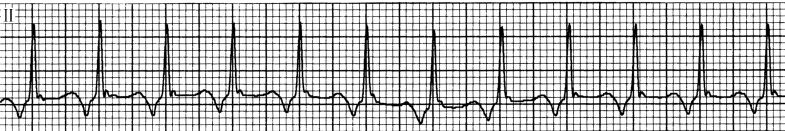
\includegraphics[width=3.28125in,height=3.66667in]{./images/Image00029.jpg}
\end{table}


\paragraph{直立性低血压的治疗}

治疗目标是预防症状复发以及晕厥造成的伤害,改善生活质量。药物诱发的自主神经功能失调可能是直立性低血压性晕厥最常见的原因,主要治疗方法是停药,仅有少数患者由于病情不能停药。引起直立性低血压最常见的药物是利尿剂和血管扩张剂,酒精也是常见的原因,其除诱发自主神经性晕厥外还可引起躯体神经系统疾病。包括对中枢神经系统的直接作用和血容量不足。主要治疗是戒酒。对于原发性和继发性自主神经功能失调的患者,了解血压调节的生理和病生理机制十分重要,治疗的主要目标是改善由于脑灌注不足导致的症状(如晕厥、先兆晕厥、意识模糊等)。尽管通过上述治疗使收缩压升高幅度不大(10~15mmHg),但可以明显改善直立性低血压的症状;使平均动脉压升高恰到好处,重新达到自主神经的调节范围内,进而可以明显改善神经调节功能。应对所有患者进行健康教育,使他们了解影响血压的因素,避免突然站起(尤其是醒后)、长时间站立、白天长时间卧位休息、用力排尿排便、过度通气、高温环境(包括热澡水、淋浴、桑拿浴)、极度用力、暴食(特别是精制的碳水化合物)、具有扩血管作用的酒精和药物。动态监测血压有助于了解白天不同环境中的血压变化,了解高血压患者药物对卧位/夜间血压的影响。扩张细胞外容量是重要的治疗目标。对无高血压的患者,应指导摄入足够的盐和水。每天达到2~3L液体和10g氯化钠。快速摄入冷开水对运动中或餐后低血压者有明显疗效;高枕位睡眠(头部抬高10°)可防止夜间多尿,维持适量的体液量及改善夜间高血压。老年患者可佩戴腹带或加压弹力袜以减轻下肢血液蓄积;有先兆晕厥时可采取交叉腿和蹲位姿势等预防措施。α受体激动剂(米多君)是慢性自主神经异常者的首选药物。氟氢可的松(0.1~0.3mg/d)可促进钠水潴留及扩张血容量,改善晕厥症状。其他治疗如去氨加压素用于伴夜尿增多者;奥曲肽用于餐后低血压,促红细胞生成素用于贫血者等。直立性低血压治疗建议见表\ref{tab4-12}。

\begin{table}[htbp]
\centering
\caption{直立性低血压的治疗建议}
\label{tab4-12}
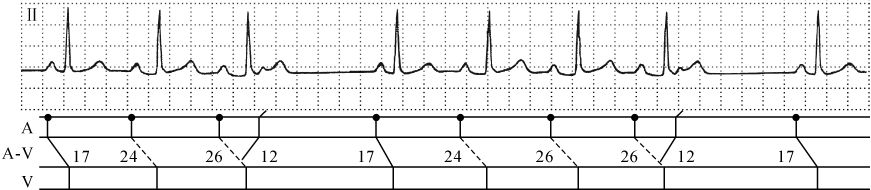
\includegraphics[width=3.27083in,height=2in]{./images/Image00030.jpg}
\end{table}

\paragraph{心律失常性晕厥的治疗}

治疗目标预防症状复发,改善生活质量,减低死亡危险。原发性心律失常与心脏本身疾病或解剖异常有关,是最常见晕厥原因之一。包括原发性窦房结功能异常(缓慢、快速心律失常)、传导系统病变、室上性心动过速和室性心动过速。这种晕厥的基础是多方面的,包括心律失常的频率、左心室的功能状态和血管的代偿作用(包括神经反射作用)。

\hypertarget{text00014.htmlux5cux23CHP1-4-4-1-3-1}{}
(1) 窦房结功能不全:

窦房结功能不全伴缓慢心律失常、或SNRT异常引起的晕厥,起搏治疗效果显著。永久起搏可明显缓解症状,但对生存率无影响。预防晕厥复发的另一主要措施是停用加重或诱发心动过缓的药物,如无合适的替代药物应行心脏起搏。

\hypertarget{text00014.htmlux5cux23CHP1-4-4-1-3-2}{}
(2) 房室传导系统疾病:

AV阻滞引起的晕厥需起搏治疗,永久右室心尖部起搏的危害已获证实,但其替代起搏位点仍有争议。AV阻滞伴LVEF下降、心力衰竭(心衰)及QRS间期延长所致者可考虑双腔起搏。

\hypertarget{text00014.htmlux5cux23CHP1-4-4-1-3-3}{}
(3) 阵发性室上性和室性心动过速:

阵发性室上性和室速或典型心房扑动引起的晕厥,应首选导管消融术。尖端扭转型室速所致的晕厥主因是应用引起QT间期延长的药物所致,应立即停药。心功能正常或轻度受损者,如出现室速伴晕厥,可考虑导管消融或药物治疗。心功能不全、室速或心室颤动伴晕厥且病因无法祛除者应植入埋藏式心脏复律除颤器(ICD)。ICD虽不能有效预防晕厥复发,但可降低猝死风险。心律失常性晕厥的治疗见表\ref{tab4-13}。

\paragraph{SCD高危患者不明原因晕厥的治疗}

其治疗目标不仅仅是防止晕厥再发,而且要治疗基础疾病和减少SCD的风险。严重主动脉狭窄或心房黏液瘤所致的晕厥可考虑手术治疗;继发于急性心血管事件如肺栓塞、心肌梗死或心包压塞者主要针对病因治疗;大多数心肌缺血所致者可采用药物和(或)血管重建;由原发性肺动脉高压或限制性心肌病引起者,一般不易纠正原发病。急、慢性冠状动脉疾病或LVEF下降均可增加死亡风险,故需评估缺血的严重程度,且如果有适应证应考虑血运重建。但血运重建并不能改善恶性心律失常引起的不良后果,因此该类患者应行电生理检查以评估有无心律失常。心衰且符合最新指南制定的ICD适应证者,无论晕厥发生机制是否明确,均应植入ICD。有研究显示,植入ICD的晕厥患者生存率明显增加;不明原因晕厥的缺血性或非缺血性心肌病伴心衰或LVEF严重下降者应植入ICD(Ⅰ类,A级);LVEF正常和电生理检查阴性者不建议植入ICD。其他类型心脏病:①肥厚性心肌病伴不明原因晕厥尤其是发作间期短(<
6个月)、相对危险度>
5的患者,其猝死风险较高;植入ICD效果明显。②约1/3致心律失常性右室心肌病(ARVC)者会发生晕厥。年轻、严重右室发育不全、左室功能障碍、多形性室速、心室晚电位、epsilon波及有猝死家族史者,如无其他病因应考虑植入ICD。③遗传性离子通道异常性心脏病常以晕厥为先兆表现,但该类患者是否应植入ICD仍有争议。SCD高危晕厥患者ICD适应证见表\ref{tab4-14}。

\begin{table}[htbp]
\centering
\caption{心律失常性晕厥的治疗建议}
\label{tab4-13}
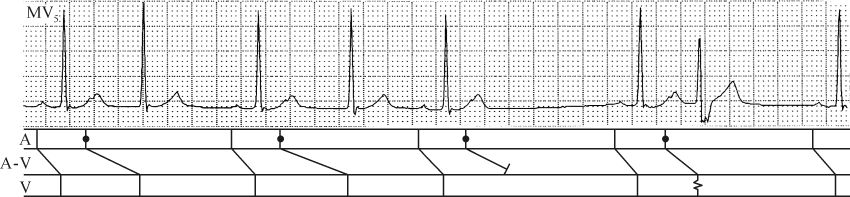
\includegraphics[width=3.29167in,height=7.86458in]{./images/Image00031.jpg}
\end{table}

\begin{table}[htbp]
\centering
\caption{SCD高危晕厥患者ICD适应证}
\label{tab4-14}
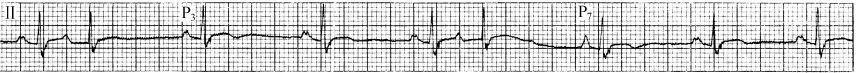
\includegraphics[width=3.3125in,height=3.55208in]{./images/Image00032.jpg}
\end{table}

\paragraph{特殊人群晕厥的处理}

\hypertarget{text00014.htmlux5cux23CHP1-4-4-1-5-1}{}
(1) 老年人晕厥:

老年人最常见的晕厥原因是OH、反射性晕厥,特别是颈动脉窦过敏和心律失常。一个患者可能有不同的机制共同作用,从而给诊断带来困难。与OH相关的住院治疗随着年龄的增加而增加,65~74岁是4.2\%,75岁以上为30.5\%。在有晕厥症状的患者之中,25\%是年龄相关的OH;其他OH主要是药物和特发性或继发性房颤所致。有OH的老年患者常有卧位收缩期高血压,并在接受多种药物治疗,给予OH药物治疗会加重卧位高血压,反之亦然。心脏抑制型颈动脉窦过敏是晕厥的原因,老年者高达20\%。血管减压型为主的颈动脉窦敏感同样常见,但是其在晕厥中的作用知之甚少。

对于老年人诊断检查和策略应注意:①老年人的OH常常具有重复性(特别是与药物或年龄相关)。因此,应反复进行OH评价,最好在早晨和(或)晕厥刚刚发生后进行。②对没有晕厥史者,即使颈动脉窦过敏不具特异性,颈动脉窦按摩检查也是特别重要的。③评价老年人反射性晕厥时,倾斜试验耐受性和安全性均很好。其阳性率与年轻人相仿,特别是在硝酸甘油激发后。④如果怀疑血压不稳定(如服药后或者餐后),24小时动态血压监测可能有帮助。⑤由于老年人心律失常发生频率高,对不明原因晕厥的老年人ILR特别有用。

\hypertarget{text00014.htmlux5cux23CHP1-4-4-1-5-2}{}
(2) 儿童晕厥:

对儿童晕厥的诊断评估与成人类似。反射性晕厥占病因学的绝大部分。但是在少数情况下,晕厥的发生是威胁生命的心律失常或心脏器质性异常所致。晕厥应该与癫痫和精神性假性晕厥鉴别,后者十分少见,但是是儿童TLOC的重要原因。

在幼童时期的两种特殊情况:①婴儿反射性晕厥发作(也叫做苍白屏气发作或反射性缺氧发作)是由短暂不愉快刺激导致的由迷走神经介导的心脏抑制所致。②窒息低氧性TLOC(发绀性呼吸停止)以哭闹时呼吸运动终止于呼气阶段为特征,从而导致发绀和通常所见的TLOC。

儿童倾斜试验的假阳性和假阴性率均较高,因此对于反射性晕厥的初步评估应持审慎态度。有报道对于健康少年儿童在静脉用药后进行倾斜试验时,先兆晕厥的比率非常高(40\%)。年轻患者首发晕厥可能为少见的、但是是威胁生命的疾病,如LQTS、Kearns-Sayre综合征(外眼肌麻痹和进行性心脏传导阻滞)、Brugada综合征、儿茶酚胺依赖性多形性VT、预激综合征、ARVC、肥厚型心肌病、肺动脉高压、心肌炎、先天性心脏病修补术后心律失常、冠状动脉异常起源。

对于具有下面情况的患儿可能提示有心脏性病因,应迅速进行心脏方面的评估:①家族史:年轻的SCD者<
30岁;家族性心脏病。②已知或可疑心脏病。③触发事件:噪音、惊吓、极端情感刺激。④运动时晕厥,包括游泳。⑤仰卧或者睡眠时无晕厥先兆,或晕厥前有胸痛或心悸。

儿童晕厥的治疗策略与成人相同。然而需要强调的是目前缺乏关于儿童反复晕厥良好设计的研究,因此药物和倾斜训练的有效性不能肯定。此外,尽管有血管迷走神经性晕厥以及长时间心脏停搏的证据,由于为一过性和良性晕厥,因此应避免安装起搏器。

总之,对儿童晕厥评估要点有几方面:①儿童期晕厥常见,绝大部分源于反射机制,很少部分是源于威胁生命的病因所致。②对良性和严重病因的鉴别主要依靠病史、体格检查和心电图。③对反射性晕厥年幼患者的治疗基石是教育并使之放心。

\hypertarget{text00014.htmlux5cux23CHP1-4-4-1-5-3}{}
(3) 驾车与晕厥:

随着轿车进入中国普通家庭,驾车与晕厥的问题显得重要起来。但是,调查显示,在有晕厥病史的患者中,交通事故的发生率低于普通人群。晕厥患者驾驶的建议见表\ref{tab4-15}。

\begin{table}[htbp]
\begin{center}
\caption{晕厥患者驾驶的建议}
\label{tab4-15}
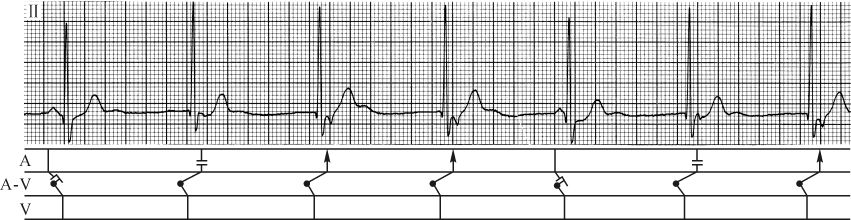
\includegraphics[width=3.27083in,height=2.86458in]{./images/Image00033.jpg}
\end{center}

{\small
注:第一组(私人驾驶者):驾驶摩托,小汽车或其他小型车辆,没有拖车;第二组(职业驾驶者):驾驶3.5吨以上汽车,除驾驶员外8座以上客车;出租车,救护车,介于私人与职业间车辆以及地方法规规定的车辆;

*:神经介导的晕厥严重且发作频繁,或正在从事高危活动;或者是复发或不可预测的高危患者
}
\end{table}

\subsection{预后}

晕厥的预后主要取决于两方面:①死亡风险及致命性事件:器质性心脏病及原发性电生理疾病是心源性猝死及晕厥患者总体死亡率的高危因素;合并联合病变的直立性低血压患者与普通人群相比,其死亡风险增加2倍;年轻且无器质性或电生理异常性心脏病的反射性晕厥患者,预后较好。大多数预后不良或死亡的患者多与基础疾病而非晕厥本身的严重程度有关。②晕厥复发及其危害:晕厥发生的次数是预测其复发的最佳指标,如诊断不明、低风险及年龄>
40岁、曾有1~2次晕厥发作史者,其复发率分别为15\%(1年内)和20\%(2年内);有3次发作史者,其复发率分别为36\%(1年内)和42\%(2年内)。


\hypertarget{text00015.htmlux5cux23CHP1-4-6}{}
参 考 文 献

Moya A,Sutton R,Ammimti F,et al. Guidelines for the diagnosis and
management of syncope(version 2009):the Task Force for the Diagnosis
and Management of Syncope of the European Society of
Cardiology(ESC).Eur Heart J,2009,30:2631-2671.

\protect\hypertarget{text00016.html}{}{}

\chapter{抽搐与惊厥}

抽搐(tics)系指全身或局部骨骼肌群非自主抽动或强烈收缩。抽搐包括痫性发作(seizure)和非痫性发作。痫性发作是脑神经元突然过度放电引起的短暂脑功能失调,患者出现全身(四肢、躯干、颜面)骨骼肌非自主强直性(持续肌肉收缩)与阵挛性(断续肌肉收缩)抽搐,引起关节运动和强直,又称癫痫发作。全面性强直-阵挛性抽搐即为惊厥发作(convulsion),常为全身性、对称性,多伴有意识障碍。

癫痫(epilepsy)则特指慢性反复发作性短暂脑功能失调综合征,具有反复性和发作性两个基本特征。癫痫持续状态(status
epilepticus)是抽搐患者最严重的表现形式之一,是指一次癫痫发作持续时间较久(>
30分钟),或癫痫频繁发作,发作间歇期意识尚未完全恢复。但研究显示较短暂的癫痫发作(<
30分钟)也可导致神经功能受损,且一旦痫性发作超过5分钟,自发终止的可能性就不大,所以建议在急诊情况下如癫痫发作超过5分钟即考虑癫痫持续状态。快速评估和控制癫痫发作是本章讨论的重点,从气道保护、神经功能稳定和寻找可能病因等三个方面积极应对,以减少其致残和死亡率。

\subsection{病因与发病机制}

抽搐的表现形式多样,主要分痫性发作和非痫性发作,前者有惊厥(全面性强直-阵挛发作)、强直性抽搐、肌阵挛发作、失神发作、自动症(automatism)等,后者见于低血钙手足抽搦、假性癫痫发作(如癔症性抽搐)等,因此其病因和发病机制非常复杂。

\subsubsection{病因}

\paragraph{癫痫和癫痫综合征}

具有特征性临床症状和脑电异常,但病因不清楚的癫痫发作,临床上倾向于基因突变和某些先天性因素所致,有明显遗传倾向;在患者神经系统中目前尚未发现有足以引起人类癫痫发作的器质性损伤或生化异常。

\paragraph{症状性癫痫}

各种明确或可能的中枢神经系统病变所致,如脑外伤、围产期损伤、脑血管病、肿瘤、中枢神经系统感染、寄生虫、遗传代谢性疾病(如低血糖)、神经系统变应性疾病、狼疮脑病等。

\paragraph{状态关联性癫痫发作}

患者癫痫发作与一些特殊状态有关,如高热、缺氧、内分泌和电解质异常(低血糖、低钠血症、高渗透压、尿毒症、肝功能衰竭)、药物与毒物、酒精和阿片类物质戒断、过度饮水、睡眠剥夺等。正常人(脑结构和功能正常)在上述特殊状态下也可出现癫痫发作,但一旦去除相关状态即不再出现癫痫发作。

\paragraph{隐源性癫痫发作}

临床表现提示症状性癫痫发作,但无特定的临床和脑电图特征,也未找到明确的病因。

上面所列主要是痫性发作抽搐的病因分类,为避免分类混乱,尚未包括非痫性发作抽搐相关病因。另外还要注意抽搐与晕厥、过度通气综合征、偏头痛、发作性睡病及各种不自主动作(如震颤、舞蹈动作、手足徐动、扭转痉挛、肌痉挛等)间的鉴别。

\subsubsection{发病机制}

抽搐的发生机制极为复杂,至今仍未阐明。目前脑组织的生理、生化方面的研究显示,抽搐发作主要机制是由大脑运动神经元的异常放电致脑功能短暂失调。该异常放电主要是神经元膜电位的不稳定引起,可由代谢、营养、皮质病变等激发,并与遗传、免疫、精神因素及微量元素等有关。具体来说,根据引起肌肉异常收缩的电兴奋信号的来源不同,可分为以下两类机制:

\paragraph{大脑功能的短暂性失调}

这是脑内神经元过度同步化放电的结果,当异常的电兴奋信号传至肌肉时,则引起广泛肌群的强烈收缩而形成抽搐。在正常情况下,脑内对神经元的过度放电及由此形成过度同步化,均有一定控制作用,即构成所谓抽搐阈。许多脑部病变或全身性疾病可通过破坏脑的控制作用,使抽搐阈下降,甚至引起抽搐。①神经元异常放电及其扩布:颅内外许多疾病,可通过不同途径影响膜电位的稳定,有直接引起膜电位降低(如低钠血症),使神经元更易去极化而产生动作电位(兴奋阈下降);间接通过影响能量代谢或能量缺乏,导致膜电位下降;神经元膜的通透性增高,使细胞外钠流入细胞内,而细胞内钾外流,因而膜电位及兴奋阈降低。②神经递质与突触传递的改变:中枢神经系统某些神经元的轴突于突触点释放抑制性递质,对神经元的过度放电及同步化也起一定控制作用。当兴奋性神经递质过多(如有机磷中毒时乙酰胆碱积聚过多)或抑制性神经递质过少(如维生素B\textsubscript{6}
缺乏时,由于谷氨酸脱羧酶的辅酶缺乏使谷氨酸转化成抑制性递质的γ-氨基丁酸减少)均可导致抽搐。③抑制系统通路受阻断:脑内有些神经元组成广泛的抑制系统,有控制神经元过度放电的作用。脑部病变除了直接损害神经元膜或通过影响脑血液供应外,也可能阻断抑制系统,使神经元容易过度兴奋。④网状结构的促去同化系统功能降低:脑干神经元放电同步化系统与网状结构的促去同化系统之间的平衡,对控制神经元的过度放电及同步化起相当的作用。

\paragraph{非大脑功能的障碍}

引起肌肉异常收缩的电兴奋信号来源于下运动神经元,主要是脊髓的运动神经元或周围运动神经元。如破伤风杆菌外毒素选择性作用于中枢神经系统(主要是脊髓、脑干的下运动神经元)的突触,使其肿胀而发生功能障碍;马钱子碱中毒引起脊髓前角细胞过度兴奋,发生类似破伤风的抽搐;各种原因的低钙血症,除了使神经元膜通透性增高外,也常由于下运动神经元的轴突(周围神经)和肌膜对钠离子的通透性增加而兴奋性升高,引起手足搐搦。

\subsubsection{儿童惊厥发病机制}

儿童惊厥(6岁以下)发生率是成人的10~15倍,儿童惊厥的发病机制有其特殊性。婴幼儿大脑皮质功能未完善/抑制差、兴奋易扩散、神经髓鞘未完全形成、神经传导分化不全、冲动易泛化、血-脑脊液屏障不良、毒物易渗入脑组织及水电解质代谢不稳定等因素是导致儿童惊厥高发生率的主要原因。相对成人而言,短暂性脑功能失调对小儿神经系统发育影响更大,一次惊厥对近记忆的一过性影响与脑震荡所致的损伤相当,而惊厥持续状态可产生严重不可逆脑损伤,小儿惊厥30分钟以上就可产生神经元缺血病变,影响小儿智力和健康。通常成人惊厥超过6小时才产生类似变化。

\subsection{诊断思路}

抽搐并不是单一疾病,而是许多疾病的严重临床表现或主要征象。因此,在诊断过程中,应综合分析各方面资料,才能明确其发生的原因。

\subsubsection{抽搐的诊断}

\hypertarget{text00016.htmlux5cux23CHP1-5-2-1-1}{}
(一) 病史

不同疾病所致的抽搐 ,其临床表现不尽相同,故详细收集病史是非常重要的。

\paragraph{明确抽搐类型}

依抽搐的形式,可分为以下两种:①痫性发作(癫痫发作);②非痫性发作。前者(尤其是全面性强直-阵挛发作,即惊厥发作)需要急诊医师快速评估和保护气道、控制癫痫发作,并积极寻找病因。而非痫性发作抽搐虽然不似前者致命,但抽搐的控制更加困难,临床重点是寻找可能病因。判断癫痫发作最重要的依据是患者的病史,如先兆症状、发作时状态及发作后意识模糊等,而不是依靠神经系统查体和实验室检查。患者发作后意识模糊状态高度提示癫痫发作。

\paragraph{了解基础疾病和用药史}

对诊断有重要参考价值。如反复发作常提示癫痫,新近发生的癫痫发作通常由于原发性神经疾病和系统性疾病或代谢紊乱所致,有外伤、感染以及内脏器官基础疾病史者提示可能为症状性癫痫。还须详细了解用药史和饮酒史,尤其是抗癫痫药物使用情况。

\paragraph{伴随症状}

对病因诊断有相当意义。

\hypertarget{text00016.htmlux5cux23CHP1-5-2-1-1-3-1}{}
(1) 症状性癫痫发作:

①颅内疾病时可伴有头痛、发热等;②阿-斯综合征抽搐时伴有心搏停止、心音及脉搏消失;③低血糖所致抽搐前多有乏力、饥饿、出汗,发作时伴有心动过速、血压升高、瞳孔散大;④子痫者伴有头痛、眼花、呕吐,可有高血压、水肿和蛋白尿;⑤嗜铬细胞瘤时伴有心跳快、气促、出汗、面色及四肢苍白、发冷、头痛、血压急剧升高、瞳孔散大;⑥尿毒症患者伴有氮质血症和酸中毒表现。

\hypertarget{text00016.htmlux5cux23CHP1-5-2-1-1-3-2}{}
(2) 低血钙性手足搐搦症:

①甲状旁腺功能减退症患者可伴有哮喘,易激动、焦虑等精神症状,皮肤粗糙,头发脱落,牙齿发育不良;②肠源性手足搐搦症患者伴有慢性腹泻;③肾病性手足搐搦症患者伴有代谢性酸中毒表现;④假性甲状旁腺功能减退症患者伴有先天畸形如矮胖、圆脸、短指。

\hypertarget{text00016.htmlux5cux23CHP1-5-2-1-1-3-3}{}
(3) 血钙正常性碱中毒性手足搐搦症:

伴有引起碱中毒的症状,如过度换气,大量呕吐或服用大量碱性药物。

\hypertarget{text00016.htmlux5cux23CHP1-5-2-1-2}{}
(二) 体格检查

导致抽搐病因众多 ,常涉及临床各科,详细系统地体检十分重要。通常包括:

\paragraph{系统查体}

重点是生命体征和有无创伤表现。但几乎体内各重要内脏器官的疾病均可引起抽搐,故须按系统进行检查。如心音及脉搏消失、血压下降或测不到,或严重心律失常,要考虑心源性抽搐;苦笑面容、牙关紧闭、角弓反张者要考虑破伤风;怀疑手足抽搦症时要查:①Chvostek征:以中指轻扣耳前面神经,可引起同侧面肌抽搐;②Trousseau征:以血压计袖带缠绕一侧上臂,打气至舒张压与收缩压之间,维持3分钟,可引起该侧手的搐搦。

\paragraph{神经和精神科查体}

有助于致抽搐病变的定性与定位。重点注意瞳孔反射、病理征、局灶神经体征、眼底情况。

\hypertarget{text00016.htmlux5cux23CHP1-5-2-1-3}{}
(三) 辅助检查

根据病史
、体检所提供的线索,选择辅助检查项目。①全身性疾病:应选择相应的检查。除了血尿粪常规外,有心电图、血液生化(血糖、尿素氮、电解质等)、血气分析、肝肾功能、内分泌功能测定、毒物分析等。②神经系统疾病:根据临床提示的病变部位和性质,选择相应的辅助检查。如脑电图、肌电图、脑脊液、神经影像学检查(头颅CT、MRI、MRA)等,近年来PET等功能影像学检查手段越来越多地被用于抽搐的病因诊断,它可实现脑局部代谢变化,辅助癫痫灶定位。

\subsubsection{抽搐的病因判断}

所有抽搐患者均应结合上述资料尽可能做出病因诊断,如为首次发作,首先须排除各种疾病引起的症状性发作,寻找可逆因素(如低血糖、低钠血症、低钙血症、药物过量等)。临床上还可根据抽搐时是否伴有意识障碍,可将抽搐分为两大类:

\hypertarget{text00016.htmlux5cux23CHP1-5-2-2-1}{}
(一) 伴意识障碍性抽搐

\paragraph{大脑器质性损害性抽搐}

其特点为:①抽搐为阵挛性和(或)强直性;②意识障碍较重,持续时间长,且多伴有瞳孔散大、大小便失禁、面色青紫等表现,多数有颅内高压表现;③脑脊液检查常有异常发现,脑电图、CT、MRI等检查有助于诊断。

\paragraph{大脑非器质性损害性抽搐}

其特点有:①意识障碍可轻可重,多数为短暂性昏迷,约在数秒至数十秒内自行恢复;②全身性疾病的表现往往比神经系统表现更明显;③无明确的神经系统定位体征;④脑脊液检查和脑电图检查多正常。

\hypertarget{text00016.htmlux5cux23CHP1-5-2-2-2}{}
(二) 不伴意识障碍性抽搐

可分为神经肌肉兴奋性增加(见于低血钙或低血镁、破伤风或马钱子碱中毒)和神经肌肉兴奋性正常(见于药物戒断反应、癔症性抽搐)两类,但以电解质紊乱(如低血钙、低血镁等)所致者较为常见。此类抽搐的特点是呈疼痛性、紧张性肌收缩,常伴有感觉异常。根据病史和临床表现常可确定这类抽搐的病因。如诊断有困难时,可测定血钙与血镁。在紧急情况下,可先静注10\%葡萄糖酸钙10ml,无效时可再静注25\%硫酸镁5~10ml。这样既有鉴别诊断的意义,又有治疗作用。

\subsubsection{临床常见抽搐}

\paragraph{癫痫发作(痫性发作)}

患者出现全身骨骼肌非自主强直性与阵挛性抽搐,引起关节运动和强直,伴或不伴意识障碍。根据临床表现可分为:①部分发作(局灶发作):单纯部分性发作(发作时无意识障碍)、复杂部分性发作(有不同程度意识障碍);②全面性发作:全面性强直-阵挛发作(即癫痫大发作,俗称惊厥,部分患者发作前有先兆,分强直期、阵挛期和痉挛后期)、强直性发作、阵挛性发作、肌阵挛发作、失神发作、失张力性发作等。

分类颇显繁杂,急诊临床重点是识别:是否是癫痫发作?是全面性发作吗?是癫痫持续状态吗?由于癫痫持续状态期间脑神经元能耗骤增,脑内pH下降,加之全身性缺氧,肌肉强烈而持久性收缩,酸性代谢产物增加,可导致脑缺氧、脑水肿甚至脑疝形成。持续状态时需要紧急保护气道、控制癫痫发作(稳定神经功能)和确定病因。

\paragraph{手足搐搦症}

以疼痛性、紧张性肌肉收缩为特征,多伴有感觉异常,见于各种原因所致的低钙血症和低镁血症。表现为间歇发生的双侧强直性痉挛,上肢较显著,尤其是在手部肌肉,呈典型的:“助产手”,即手指伸直内收,拇指对掌内收,掌指关节和腕部屈曲;常有肘伸直和外旋。下肢受累时,呈现足趾和踝部屈曲,膝伸直。严重时可有口、眼轮匝肌的痉挛。发作时意识清,Chvostek征和Trousseau征阳性。

\paragraph{破伤风}

破伤风杆菌外毒素-破伤风痉挛毒素可阻断脊髓的抑制反射,脊髓前角运动神经元兴奋性增高,同时也使脑干广泛脱抑,导致肌痉挛、肌强直,表现为张口困难、牙关紧闭、腹肌僵硬、角弓反张。肌强直的特点是在抽搐间歇期仍存在,肌抽搐可为自发性,亦可因外界刺激而引起,面肌强直和痉挛形成苦笑面容,咽肌和膈肌受累导致饮水困难和呛咳。破伤风的抽搐虽可十分严重,但神志清楚。外伤史有助于疾病的诊断。

\paragraph{癔症性抽搐}

属一种功能性动作异常。患者多为年轻女性,在精神因素刺激下发作,表现为突然倒下,全身僵直、牙关紧闭、双手握拳,其后不规则的手足舞动,常杂以捶胸顿足、哭笑叫骂等情感反应,发作持续数分钟至数小时。其特点是:①抽搐动作杂乱,无规律可循,不指向神经系统的某一定位损害;②无瞳孔变化和病理反射;③常伴有流泪、过度呼吸、眼活动频繁和眨眼过度;④无舌头损伤及大小便失禁;⑤发作时脑电图正常;⑥暗示或强刺激可终止其发作。

\paragraph{发热惊厥}

惊厥发作的典型临床表现是意识突然丧失,同时急骤发生全身性或局限性、强直性或阵挛性面部、四肢肌肉抽搐,多伴有双眼上翻、凝视或斜视。最常见于幼儿,发病多在6个月至6岁之间,以3岁以前小儿多见。最常见于上呼吸道感染、扁桃腺炎,少数见于消化道感染或出疹性疾病,约一半患儿有家族史,提示同遗传因素有关。惊厥的发生常与发热相关,但热度高低并不与之呈正相关。发作形式多为单次,全身性强直、阵挛性发作,持续时间在30秒钟以内,一般不超过10分钟,脑电图有节律变慢或枕区高幅慢波,在退热后1周内消失。可能每年有一至数次同样发作,但若无脑损害征象,并不导致癫痫。

\paragraph{中毒性抽搐}

最常见于急性中毒。其发生抽搐的主要机制:①直接作用于脑或脊髓,使神经元的兴奋性增高而发生抽搐。大多是药物的过量,如戊四氮、贝美格(美解眠)、樟脑、印防己毒素、阿托品、麦角胺、丙米嗪、氯丙嗪、白果等;②中毒后缺氧或毒物作用,引起脑代谢及血循环障碍,形成脑水肿。见于各种重金属、有机化合物、某些药物和食物的急性重度中毒。临床多呈全身性肌强直阵挛性发作,少数也可呈局限性抽搐,有的可发展为癫痫状态。常合并其他中毒表现。马钱子碱(士的宁)中毒的临床表现类似破伤风,仅在抽搐间隙无持续性的肌痉挛。

\paragraph{心源性抽搐}

是指各种原因引起心排出量锐减或心脏停搏,使脑供血短期内急剧下降所致的突然意识丧失及抽搐,也称昏厥性抽搐。常见于严重心律失常、心排血受阻的心脏病或某些先天性心脏病、心肌缺血、颈动脉窦过敏、血管抑制性昏厥、直立性低血压等。其抽搐时间多在10秒钟内,较少超过15秒钟,先有强直,躯体后仰,双手握拳,接着双上肢至面部阵挛性痉挛,伴有意识丧失,瞳孔散大、流涎,偶有大小便失禁。发作时心音及脉搏消失,血压明显下降或测不到。脑电图在抽搐时呈电位低平,其后为慢波,随意识恢复后逐渐正常。

\paragraph{急性颅脑疾病相关抽搐}

颅内感染、颅脑损伤、急性脑血管病是导致症状性癫痫发作的主要因素。抽搐多为痫性发作,且多与病变程度相平衡,有的随着颅脑病变的加剧抽搐频繁、加剧,甚至发展为癫痫持续状态。抽搐仅是临床表现之一,大多还有脑局灶或弥散损害的征象,如头痛、呕吐、精神异常、偏瘫、失语、意识障碍、脑膜刺激征等表现。脑脊液检查及CT、MRI等检查可有相应的阳性发现。

\paragraph{药物戒断反应}

长期连续服用安眠药,主要是巴比妥类安眠药患者,常产生药物依赖性甚至成瘾,在突然停药后可引起严重戒断反应,表现为异常兴奋,焦虑不安、躁动甚至发生四肢抽搐或强直性惊厥。阿片类药物的戒断反应较安眠药更严重而持久。处理主要是对症治疗,并逐渐停药。

\paragraph{代谢、内分泌异常所致的抽搐}

许多代谢、内分泌疾患,可因电解质紊乱,能量供应障碍等,干扰了神经细胞膜的稳定性,而出现抽搐,同时有明显代谢、内分泌异常的临床表现。如各种疾病所致的低钙血症、低钠血症、低镁血症、碱中毒、低血糖症(血糖<
2mmol/L)等,均可致抽搐。

\subsection{处理原则}

\subsubsection{急诊处理思路}

\paragraph{他人发现患者抽搐、晕厥、昏迷?}

急诊抽搐患者往往是被他人送来急诊就诊,而旁观者很难分别是抽搐,还是晕厥或昏迷,这时急诊医师不要仓促下结论患者是癫痫发作,具体分析思路见图\ref{fig5-1}。

\paragraph{考虑癫痫发作的分析和处理思路}

在急诊抽搐患者处理的难点正是如何判断是否是癫痫发作,可通过以下线索来分析判断:强直-阵挛性运动病史、大小便失禁、发作后意识模糊、舌体咬伤等。在急诊如经过初始评估考虑患者为癫痫发作时,临床分析思路参考图\ref{fig5-2}。但患者的处理依然优先要考虑初始评估、稳定(保护气道)、神经功能稳定(控制癫痫发作)、寻找病因这一处理流程。

\subsubsection{保护气道}

首先应将患者置于安全处,解开衣扣,去除义齿,清除口腔异物,保持呼吸道通畅。有意识障碍者,将身体或头须转向一侧,以利口腔分泌物流出,防止吸入肺内致窒息或肺炎。分泌物较多者,准备好负压吸引器,随时吸痰。必要时给氧,气管切开或气管插管给予人工呼吸,维持正常的通气功能。

\subsubsection{快速评估和稳定}

重症病例应进行血压、心电图和脉搏氧饱和度等监测,急查血电解质和动脉血气,并予吸氧,建立静脉通路。若有异常发现,应及时处理。如给予抗抽搐药物不能终止癫痫发作,需作好气管插管准备。

低血糖是最常见引起痫性发作的代谢性因素,另一方面,要注意长时间抽搐也可致低血糖,低血糖症者,应给予50\%葡萄糖50m1,静脉推注(5分钟内);有糖尿病高血糖者,应给予胰岛素治疗。

疑有营养不良症者,应给予维生素B\textsubscript{l}
l00mg肌肉注射或静脉注射;怀疑异烟肼过量者应用维生素B\textsubscript{6}
;有低血钙症者,应给予10\%葡萄糖酸钙10ml或10\%氯化钙10m1,缓慢静脉注射(5分钟以上),必要时重复给药,但24小时给予的总钙量,一般不超过25mmol。

\begin{figure}[!htbp]
 \centering
 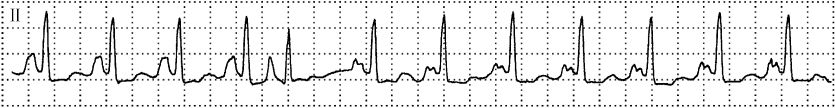
\includegraphics[width=5.88542in,height=6.04167in]{./images/Image00034.jpg}
 \captionsetup{justification=centering}
 \caption{他人发现抽搐、晕厥或昏迷患者分析思路}
 \label{fig5-1}
  \end{figure} 

\begin{figure}[!htbp]
 \centering
 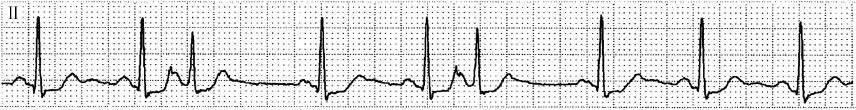
\includegraphics[width=4.77083in,height=4.34375in]{./images/Image00035.jpg}
 \captionsetup{justification=centering}
 \caption{癫痫发作的分析和处理思路}
 \label{fig5-2}
  \end{figure} 

\subsubsection{控制抽搐发作}

一旦确定是全身强直-阵挛性发作(癫痫大发作)或癫痫持续状态,及时控制抽搐是临床治疗的关键。癫痫持续状态处理流程见图\ref{fig5-3},有很强的时间紧迫性,目标是在神经功能受损前控制癫痫发作(理论上是在20分钟至1小时内控制抽搐发作)。应优先选择抗惊厥作用强、吸收快、分布半衰期长、排除半衰期短、无心肺和意识抑制作用,能肌肉注射、静脉注射和毒副作用低的药物。癫痫持续状态的药物治疗应根据患者的个体情况及时适度地应用,力争在最短的时间内终止癫痫发作,然后给予维持治疗。抽搐时切记勿强行固定四肢(否则易导致骨折、脱臼),也不要在抽搐时往患者嘴里塞牙垫、毛巾等物。抽搐停止后应加强监护,以防自伤、误伤、伤人、毁物等。

\paragraph{地西泮(安定)}

为一线控制癫痫发作药物,适用于各年龄段。见效快,半衰期短(0.5~4小时)。成人首次剂量10~20mg,按1~5mg/min缓慢静脉注射,有效而复发者,30分钟后可重复应用,或在首次用药后将安定20~40mg加入10\%葡萄糖液100~250ml中缓慢静滴,10~20mg/h,用于维持疗效,视发作情况控制滴注速度和剂量,24小时总剂量不宜超过120mg(注:在控制癫痫发作时,地西泮剂量理论上来说没有上限)。无论地西泮的疗效如何,宜与苯妥英钠或苯巴比妥合用,预防抽搐再次发作。

儿童地西泮剂量每次0.25~0.5mg/kg静推,速度1mg/min,婴儿不超过2mg/次,幼儿不超过5mg/次。5~10岁儿童1mg/岁,儿童一次用量不超过10mg。新生儿及婴儿亦可用地西泮,每次0.5~1mg/kg肛管给药。

其他苯二氮{}
类制剂亦可选用,如劳拉西泮(氯羟安定),与地西泮相比抗惊厥作用强5倍,作用时间长3~4倍,半衰期12~16小时。静脉注射2~5mg/次(0.1mg/kg,速度2mg/min),80\%以上病例可在2~3分钟内终止发作,特别推荐在酒精戒断相关癫痫发作患者中使用。最新研究显示静脉注射劳拉西泮在控制抽搐和预防复发方面均优于地西泮。氯硝西泮抗惊厥作用是地西泮的5倍,半衰期22~32小时,静脉注射1~4mg/次,60\%病例可控制发作24小时。

如果尚未给患者建立静脉通路,地西泮可以通过直肠、气管套管内、骨髓腔内等途径给药。苯二氮{}
类药物有呼吸抑制、心动过缓和低血压、酸中毒等副作用,应用时需随时评估气道,脉搏氧饱和度降至90\%以下或呛咳作呕反射消失者,应考虑予气管插管。

\paragraph{苯妥英钠}

控制成人癫痫发作二线治疗药物,无呼吸抑制,静脉给药能迅速达到脑内有效浓度。常用为150~250mg/次(20mg/kg),生理盐水溶解,缓慢静脉注射(1分钟小于50mg),半小时后可重复给药(100~150mg)。严重病例可加大用药剂量。儿童用量为250mg/m\textsuperscript{2}
。因为有低血压和心律失常等副作用,胃肠外给药速度不要过快,用药期间应密切观察,或行心电图和血压监测。

\paragraph{苯巴比妥钠}

控制成人癫痫发作三线治疗药物。若足量的苯妥英钠仍不能控制抽搐发作,应立即给予苯巴比妥钠治疗。按10mg/kg静脉缓慢注射(50~100mg/min),直至发作停止,可再追加50mg,剩余部分可行肌肉注射。呼吸抑制和低血压是其常见副作用,用药前应准备气管插管和人工辅助呼吸通气。注射过程中需密切观察呼吸情况,如有抑制呼吸现象应立即停止注射,并作人工辅助通气。注意对儿童来说苯巴比妥钠是二线药物,而苯妥英钠是三线药物。

\begin{figure}[!htbp]
 \begin{center}
 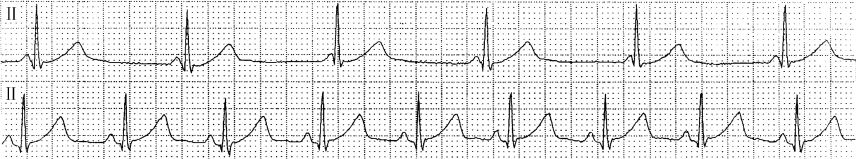
\includegraphics[width=4.11458in,height=5.28125in]{./images/Image00038.jpg}
 \captionsetup{justification=centering}
 \caption{癫痫持续状态处理路径}
 \label{fig5-3}
 \end{center}

 {\small
 注:苯巴比妥剂量在国内有限制:一次极量为0.3g,一日极量为0.5g
 }
 \end{figure} 

\paragraph{其他药物}

如上述治疗无效,应考虑请神经专科医师会诊,并试用下列药物:①丙戊酸:控制癫痫发作有效药物。推荐剂量是15~20mg/kg或600~1200mg/d,分2~3次口服,其临床安全性良好,但注意在肝功能不全患者中禁用。②副醛:成人8~10ml、儿童0.3ml/kg,用植物油稀释后保留灌肠。代谢性酸中毒、肺出血、心血管抑制和直肠炎等是常见的副作用,应注意观察。③利多卡因:成人用1\%的利多卡因10ml,以20mg/min速度匀速静注。可降低心输出量,有充血性心力衰竭和肝损害减量。④10\%水合氯醛:成人20~30ml、儿童0.3ml/kg保留灌肠。

\paragraph{全身麻醉}

处理仍无效者,可考虑收入ICU,静脉持续泵入咪达唑仑、丙泊酚等药控制癫痫发作,但其临床疗效有待进一步验证,也试用下列药物全身麻醉:①戊巴比妥:15mg/kg缓慢静脉注射,然后以0.5~1mg/(kg•h)维持。②硫喷妥钠:15mg/kg静脉缓慢推注,继以5mg/(kg•h)静脉注射维持。脑内的半衰期低于30分钟。③异戊巴比妥:200~1000mg静脉缓慢推注。

\subsubsection{病因治疗}

病因治疗是根本。如中毒性抽搐,应尽速彻底清除毒物和应用特效的解毒剂;急性感染性疾病所致者选用相应有效的抗生素,破伤风者须应用破伤风免疫球蛋白和抗生素(甲硝唑);高热惊厥,首先降温,使体温控制在38℃以下;低血糖发作应立即静注50\%葡萄糖液;水电解质平衡失调应分别纠正所缺少的钙、钠、镁;心源性抽搐者,应尽快建立有效循环,提高心排出量,治疗原发病;对肝肾功能衰竭者,改善并恢复其功能至关重要;颅内肿瘤、血肿、脓肿、脑寄生虫病及各种原因的脑水肿引起抽搐者,必须脱水降颅内压,必要时外科手术治疗。

\subsubsection{对症治疗}

癫痫持续状态l小时以上者,即有发生脑缺氧脑水肿的可能性,应酌情给予地塞米松、20\%甘露醇或利尿剂治疗,为了预防继发感染,应给予抗生素治疗。有高热者应给予降低过高体温处理。严重抽搐发作时,还可出现酸中毒、电解质紊乱、横纹肌溶解等并发症,进而又加重抽搐发作,甚至危及生命。临床上在控制癫痫发作的同时,应注意寻找并处理并发症。必须注意维持呼吸、循环、体温、水电解质平衡,保证供氧,供给充足热量,避免缺氧及缺血性脑损害。


\hypertarget{text00017.htmlux5cux23CHP1-5-4}{}
参 考 文 献

1. John Marx. Rosen's Emergency Medicine. 7th ed. Mosby,2009:113

2. Tintinalli JE. Emergency Medicine:A comprehensive study guide.6th
ed. McGraw-Hill,2004:1409

3. Rowland LP. Merritt's Neurology. 11th ed. Lippincott Williams
&Wilkins,2005:13

4. Pillow MT. Emergency Medicine. emedicine(http://emedicine.
medscape.com)updated Nov 9,2010

5. Huff JS. Emergency medicine clinics of North
America.2011,29(1):1-158

\protect\hypertarget{text00018.html}{}{}

\chapter{瘫 痪}

本章叙述的瘫痪(paralysis)是指随意肌收缩功能不全而言。其不完全障碍形成的肌力减退,属不完全性瘫痪;其完全障碍形成的随意肌收缩不能,属完全性瘫痪。本文叙述急性瘫痪的诊断与其处理原则。

\subsection{各型瘫痪的临床特征}

按病损部位不同,可将瘫痪分为肌源性、神经-肌接点性、下运动神经元性或上运动神经元性,其临床表现各具特征。现予分述如下:

\subsubsection{肌源性或神经-肌接点病损性瘫痪的临床特征}

肌源性瘫痪是指肌肉本身病变导致肌肉收缩障碍,从而引起程度不等的瘫痪而言。神经-肌接点病损性瘫痪是指神经-肌接点的递质因素或递质受体病变所引起的肌肉收缩无力而出现的瘫痪而言。

\paragraph{瘫痪分布}

大多对称,多以肢体近端为重,不符合神经支配规律。

\paragraph{肌束震颤}

通常没有。

\paragraph{肌肉萎缩}

随病程进展,出现病肌萎缩,但不出现于疾病的急性期。

\paragraph{牵张反射}

由于运动效应器病损,致紧张性牵张反射(表现为肌张力)与位相性牵张反射(表现为腱反射)均见降低。

\paragraph{病理反射}

病理反射是上运动神经元性瘫痪的特征,因此,通常不见于肌源性或神经-肌接点病损性瘫痪。

\paragraph{实验室检查}

肌细胞病变时出现血肌酶如肌酸磷酸激酶等升高;肌电图呈肌病性变;肌肉活检证实各种肌肉疾病的特征性改变。神经-肌接点病损性瘫痪时,通常血肌酶变动不明显,肌电图检查显示特征性改变。

\subsubsection{下运动神经元性瘫痪的临床特征}

\paragraph{瘫痪分布}

主要是小组肌肉或单块肌肉的瘫痪,其分布符合脊髄节段或周围神经支配的规律。

\paragraph{肌束震颤}

束颤是下运动神经元性瘫痪的特征之一,但是很少见于瘫痪的急性病期。随意肌失神经支配后,在其足板附近的肌膜上,烟碱型乙酰胆碱受体大量增生,以致血循环中存在着的小量乙酰胆碱,足以引起肌纤维的自发性收缩而在肌电图上显示为纤维颤动(纤颤)电位。纤颤电位通常见于骨骼肌失神经支配后1~3周。当整个肌束有类似变化时,就出现肉眼可见的束颤。在确认束颤与下运动神经元病变有关前,必须除外良性束颤与可能含有束颤的其他疾病如抗胆碱酯酶药物过量与电解质紊乱等。

\paragraph{肌肉萎缩}

通常始于失神经支配1~2周后。是其蛋白代谢呈负平衡的结果。

\paragraph{牵张反射}

由于反射通路受阻而致肌张力、腱反射均见减退。睡眠、昏迷或小脑病变时,也见牵张反射减退,诊断时应注意识别。

\paragraph{病理反射}

病理反射是上运动神经元性瘫痪的病征,不见于下运动神经元性瘫痪。

\paragraph{实验室检查}

血肌酶大多正常,在有的急性疾病如急性感染性多发性神经根神经炎时,或见血肌酸磷酸激酶轻度增高。肌电图示去神经性变。肌肉活检呈失神经性变。

\subsubsection{上运动神经元性瘫痪的临床特征}

\paragraph{瘫痪分布}

瘫痪分布符合神经解剖的规律,通常表现为肌群或肢体的瘫痪。

\paragraph{肌束震颤}

瘫肌无肌束震颤。

\paragraph{肌肉萎缩}

上运动神经元病变通常不影响下运动神经元对肌肉的营养作用,故瘫肌不见萎缩。但久瘫后,瘫肌可出现失用性萎缩,这种萎缩自然不见于急性病肌。

\paragraph{牵张反射}

上运动神经元病损时,瘫肌牵张反射增强,表现为瘫肌张力增高,反射增强。但是,在病损急性期,因参与瘫肌牵张反射的下运动神经元突然失去上级运动神经元的调控而进入阻抑状态,牵张反射因之消失,届时,瘫肌张力降低,腱反射难以引出,是属脊髓休克状态。

\paragraph{病理反射}

锥体系抑制原始的屈曲回缩反射。锥体系病损时,屈曲回缩反射失去抑制,从而在上肢可能出现霍夫曼(Hoffmann)征,在下肢可见跖反射伸性或(与)巴宾斯基(Babinski)征,是上运动神经元性瘫痪的病理征,亦即病理反射,但同样不见于脊髓休克期。值得注意的是,这种征象尚可见于锥体系尚未发育完全的婴儿,也可见于深睡、昏迷、全身麻醉与癫痫大发作后的短时期内;此时,这种征象通常是双侧性的。

\paragraph{实验室检查}

血肌酶、肌电图与肌肉活检的诊断价值不大。

\subsection{诊断思路}

\subsubsection{确认真性瘫痪}

为确认真性瘫痪,需与失用、骨关节病引起的随意运动障碍以及癔症性瘫痪等鉴别。

失用是指随意肌没有瘫痪,但运用不能。通常是由大脑特定功能部位的病损,影响了获得性技能的回忆能力所致。

小脑病损时,可能合并受累部位肌力减退,但总以小脑共济失调为主。震颤麻痹时,病肢可能乏力,但通常少有肯定肌力减退,且病肌张力呈齿轮状增高,尚伴震颤、运动迟缓、表情呆滞与瞬目动作减少等,易于识别。严重的舞蹈症可能合并有轻瘫,此时,病肢原有的舞蹈动作减弱,甚至消失,是为瘫痪性舞蹈病,结合舞蹈动作与受累肢体肌张力降低,可资鉴别。骨、关节病时,随意运动可能受限,但不属真性瘫痪,依骨、关节病史,保护体位,局部关节肿胀、按疼,被动活动受限、致痛,帮助识别。

癔症性瘫痪,也有起病快的,患者以青年女性为多。病前常有心理因素。瘫痪分布不一,以单瘫、截瘫较为多见;瘫痪程度可能时有变动,时轻时重,具暗示性;可伴富于情感色彩的精神症状;在神经系统体征方面,除可能测得瘫痪肢体在被动活动时阻力有所增加外,多不见其他病征。患者的癔症性格与类似的发作既往史有助诊断。需要注意的是:必须在排除器质性病因后才能考虑诊断。

\subsubsection{识别瘫痪属性}

参考前述各类瘫痪的临床特征,可以确定瘫痪的属性。但在确认急性瘫痪的属性时,必须注意:①患者是否处于脊髓休克状态。脊髓休克期,受影响的运动区呈下运动神经元性瘫痪的病征,即瘫痪肌肉张力降低,反射消失,没有病理反射。②在下运动神经元性瘫痪的急性期,瘫痪肌肉通常不显示肌束震颤与肌肉萎缩。③在肌原性瘫痪的急性期,同样没有肌肉萎缩可见。因此,在判断急性瘫痪的属性时,除瘫痪肌肉的分布外,神经系统其他病征、肌肉病征、必要的实验室检查与详尽的病史资料是不可或缺的。

\subsubsection{推测诊断}

可以将瘫痪作为考虑诊断的引线。但必须强调:只有结合病史与体征(包括神经系统其他阳性体征),进行综合分析,才能较为正确地设想可能的疾病,进而按需进行相关的辅助检查,以使诊断更臻完善。

下面就瘫痪的部位与属性,按项列举常见的急性疾病,以供诊断参考。

\paragraph{眼肌瘫痪}

眼肌瘫痪的主要临床表现为斜视、眼球运动障碍,或伴睑垂、瞳孔散缩异常等。

\hypertarget{text00018.htmlux5cux23CHP1-6-2-3-1-1}{}
(1) 肌源性或神经-肌接点病损性眼肌瘫痪:

急性起病者少见,偶见于急起的重症肌无力、急起的甲状腺毒性肌病、有机磷中毒的中间综合征与生物毒如蛇毒中毒、肉毒中毒等。

\hypertarget{text00018.htmlux5cux23CHP1-6-2-3-1-2}{}
(2) 下运动神经元性眼肌瘫痪:

可分为脑神经病变与核性病变两类:

\hypertarget{text00018.htmlux5cux23CHP1-6-2-3-1-2-1}{}
1) 脑神经病变 :

可依次分为单动眼神经麻痹、单滑车神经麻痹、单展神经麻痹或眼部多脑神经麻痹。①单动眼神经麻痹:病侧睑垂,正视时,眼球外偏略向下;眼球向上、向内与向下活动受限,并有相应复视;可伴瞳孔扩大。睑板肌由交感神经支配,其功能受损时,可致轻度睑垂,但请患者充分上视时,又见上睑上抬满意,双侧眼裂基本对等,是为假性睑垂,应注意识别。急性动眼神经麻痹可见于脑动脉瘤膨胀压迫动眼神经,也可见于痛性眼肌瘫痪、眼肌瘫痪性偏头痛、糖尿病性动眼神经麻痹、颅脑外伤、垂体肿瘤囊变或出血、肉毒中毒、白喉性多神经病等病况时。②滑车神经麻痹:单独滑车神经麻痹罕见,尤其是急性起病者。③展神经麻痹:正视时,病侧眼球偏处内收位,眼球向外活动受限,向受损侧侧视时出现复视。可见于颅内动脉瘤突然扩张的压迫、脑外伤、急性颅内压增高,转移性癌肿(尤其需要注意的是鼻咽癌)、糖尿病性展神经麻痹或特发性展神经麻痹等。④眼部多脑神经麻痹:此处是指合并动眼、滑车、展神经麻痹,按各脑神经受损程度不等,综合出现各该脑神经受损时的病征,轻重不一。可见于海绵窦病变、痛性眼肌麻痹、眼肌麻痹性偏头痛、颅脑外伤、Fisher综合征或急性出血性结膜炎引起的脊髓灰质炎样运动瘫痪等。

\hypertarget{text00018.htmlux5cux23CHP1-6-2-3-1-2-2}{}
2) 核性病变 :

核性病变常导致分离性眼肌瘫痪,即同一神经如动眼神经支配的各眼外肌呈非同步瘫痪;以双侧病损为多见,届时,两侧眼球活动的瘫痪程度与范围不一定相等,可合并会聚障碍,眼内肌功能可能保持,随眼球活动受限而出现相应复视。可见于脑干血管性病变、Wernicke脑病等。

\hypertarget{text00018.htmlux5cux23CHP1-6-2-3-1-3}{}
(3) 上运动神经元性眼肌瘫痪:

核上性病变引起双眼同向活动障碍,或称凝视麻痹。即两眼不能向一侧,或向上、向下凝视,由于两眼视轴相称,不致造成复视。

两眼侧视中枢在大脑额中回后部,其活动也受同侧枕前区侧视中枢影响;下级侧视中枢在脑桥,归属于脑桥旁正中网状结构。额中回后部的侧视中枢遭破坏时,由于对侧侧视中枢的活动而致两眼向病灶侧凝视,可见于脑血管意外、脑炎、脑外伤、脑瘤等疾病时。一侧脑桥侧视中枢遭破坏时,两眼不能向病灶侧活动而向病灶对侧凝视;多见于脑血管意外、脑桥肿瘤、多发性硬化等。脑桥病变若累及两侧凝视中枢,导致双侧性凝视麻痹。枕叶病变时,可致双眼的跟随动作消失,引起自发性定视。

垂直性凝视中枢拟在中脑。垂直性凝视麻痹以两眼向上凝视受限为多见,常由中脑上丘水平的盖前区病损导致,可见于包括蛛网膜下腔出血在内的脑血管意外等病况时。有双侧额中回病损也可引起垂直性凝视麻痹。

\paragraph{面肌瘫痪}

面肌瘫痪指面部表情肌瘫痪。①肌源性或神经-肌接点病损性面肌瘫痪:急性起病的十分罕见。②下运动神经元性面肌瘫痪:无论面神经本身或面神经核病变,均损及病侧全部面肌活动,表现为病侧皱额纹明显减退或消失,闭眼不紧或露白,鼻唇沟浅平,露齿不全,口角歪向健侧,病侧口轮匝肌无力致吹口哨不能、鼓气自瘫侧口角破漏、食物滞留病侧颊腔;核性病变者,常伴同侧眼球外展麻痹或(与)其他脑干病征,属脑干病变范畴。单侧面神经麻痹多为特发性面神经麻痹,也见于急性炎症性脱髓鞘性多发性神经病、面神经外伤、肉毒中毒、Lyme病、三氯乙烯中毒(三氯乙烯中毒的神经毒征涉及多脑神经,在瘫痪方面,以面神经与动眼神经病征为主)与急性化脓性中耳炎时。核性病变可见于基底动脉血栓形成、脑桥出血、脑干型脊髓灰质炎或急性出血性结膜炎引起的脊髓灰质炎样运动瘫痪等时。③上运动神经元性面肌瘫痪:即中枢性面瘫,表现为病灶对侧下半面部表情肌功能障碍,致鼻唇沟变浅、口轮匝肌无力、露齿时口角歪向健侧,而皱额活动不受影响,两侧额纹对称。患者常伴与病灶关连的其他病征如偏瘫等。多见于脑血管意外、脑炎、脑静区肿瘤囊变或出血等时等。

\paragraph{球肌瘫痪}

球肌,又称延髓肌,是指由舌咽、迷走、副、舌下神经所支配的随意肌。球肌瘫痪,导致构音障碍,甚或失音;吞咽困难、咳呛,甚或反流,提腭运动受限,或见喉结上提不全,舌位不正,活动受障。咽反射减退或亢进。

\hypertarget{text00018.htmlux5cux23CHP1-6-2-3-3-1}{}
(1) 肌源性或神经-肌接点病损性球肌瘫痪:

常两侧对称受损,出现上述病征,因效应器受损,咽反射减退。可见于急性的重症肌无力、多发性肌炎、急性甲状腺毒性肌病与有机磷中毒后的中间综合征或生物毒素如蛇毒中毒等。

\hypertarget{text00018.htmlux5cux23CHP1-6-2-3-3-2}{}
(2) 下运动神经元性球肌瘫痪:

可分为脑神经病变与核性病变两类。

1)
脑神经病变多见于各有关脑神经出颅腔后,在其径路上受损。单神经病损,较为少见,其病因常与外伤有关。①舌咽神经受损:舌咽神经的运动纤维支配茎咽肌。茎咽肌的功能是吞咽时提升与拓宽咽部,但其作用较小,以致在临床工作中常难以察觉其瘫痪,尤其是在单侧受损时;咽反射可能降低,这是因为咽反射的传入径路是由舌咽神经控制的。可见于颅底骨折,但单侧单独受损很少见。②迷走神经受损:迷走神经运动干司理除软腭张肌与茎咽肌以外的所有咽、喉、软腭肌,是控制软腭与咽喉部的主要运动神经。声带肌由迷走神经的分支喉返神经控制。迷走神经受损时,可出现发音、构音、吞咽障碍,悬雍垂偏向健侧、病侧提腭不全、咽反射减退,或伴声带内收障碍而致声音嘶哑。在有些病例,由于病损部位之故,软腭活动尚好,但因下咽缩肌瘫痪,致喉结运动受限。迷走神经损伤可见于颅底骨折、颈部外伤或其他颈部手术如甲状腺手术损及喉返神经等病况时。病损多为单侧,双侧者少见。双侧喉返神经受损时,咳嗽反射减退,甚或消失;声带处于尸体位,导致嘶哑,甚至失音;又可因声带开放不全而致呼吸困难、喘鸣而需手术治疗。③副神经受损:受副神经支配的胸锁乳突肌瘫痪时,颈向病损对侧转动无力;双侧胸锁乳突肌瘫痪时,颈前屈无力。斜方肌瘫痪时,病侧肩垂,耸肩受限。副神经病损常见于颈部手术伤、枪伤、刺伤、颈椎骨折脱位。④舌下神经受损:舌下神经支配所有牵引舌部的舌内、舌外肌群。当一侧舌下神经受损,舌在口腔内原位时,舌尖偏向健侧;伸舌时,舌尖偏向患侧。由于急性病损时舌肌不显示束颤与萎缩,因此,只能借病史与并存的其他神经系体征帮助确认其下运动神经元性瘫痪。所幸的是单一舌下神经急性病损,除外伤性外,仅偶见于脊髓前动脉血栓形成。急性双侧舌下神经麻痹,很为罕见,届时,除不能伸舌、不见舌部活动外,更有构音障碍、进食困难。⑤多球部脑神经受损:根据受累脑神经的多少与受损程度,组合出现有关脑神经的上述病征,多少不一,轻重不等。可见于急性炎症性脱髓鞘性多发性神经病、白喉性多神经病或外伤如颅底或颈静脉孔枪弹伤等。

2) 核性病损时
,按受累范围,产生相应脑神经的有关病征,大多合并其他脑干征。多见于椎-基底动脉系统的血管性疾病,偶见于脑干型脊髓灰质炎或急性出血性结膜炎引起的脊髓灰质炎样运动瘫痪等。

\hypertarget{text00018.htmlux5cux23CHP1-6-2-3-3-3}{}
(3) 上运动神经元性球肌瘫痪:

即核上性球肌瘫痪。病损在皮质运动区的颈、咽喉与舌部到第Ⅸ、Ⅹ、Ⅺ与Ⅻ对脑神经运动核的径路上的任何部位。在这四对脑神经的运动核中,除支配颏舌肌的运动核主要受对侧皮质延髓束支配外,余均受双侧支配。因此,其单侧皮质延髓束受损仅致病灶对侧的颏舌肌瘫,表现为伸舌时,舌尖偏向病灶对侧,这种征象多见于合并偏瘫、偏侧感觉障碍时,好见于脑血管意外、脑炎、急性播散性脑脊髓炎等疾患时。双侧皮质脑干束病损,导致假性延髓性麻痹,表现为构音不清、吞咽困难、进食反流、舌活动不灵活与提腭活动减退,但咽反射亢进。藉咽反射活跃,或伴强哭、强笑,与真性延髓性麻痹鉴别。假性延髓性麻痹的患者常伴中枢神经系统的其他病征如双侧皮质脊髓束征、失语、智力减退等。常为多次脑血管意外发作的后遗症,因此,少见于首次脑血管意外的急性状态。

\paragraph{单瘫}

单瘫是指一个肢体的瘫痪。

\hypertarget{text00018.htmlux5cux23CHP1-6-2-3-4-1}{}
(1) 肌原性或神经-肌接点病损性单瘫:

少见。

\hypertarget{text00018.htmlux5cux23CHP1-6-2-3-4-2}{}
(2) 下运动神经元性单瘫:

一侧颈\textsubscript{5~8} 与胸\textsubscript{1}
脊髓前角、前根或臂丛病变可引起同侧上肢的下运动神经元性单瘫。一侧腰\textsubscript{1}
~骶\textsubscript{2}
脊髓前角、前根或腰骶丛病变时可引起同侧下肢的下运动神经元性单瘫。①单纯前角病变引起的单瘫:可见于脊髓灰质炎(以累及下肢近端肌为多见)。②单纯急性前根病变引起的单瘫:少见。③神经丛病变引起的单瘫:在上肢可见于急性臂丛神经炎与包括产伤在内的臂丛神经损伤。在下肢单瘫较为少见。

\hypertarget{text00018.htmlux5cux23CHP1-6-2-3-4-3}{}
(3) 上运动神经元性单瘫:

其基础为对侧大脑皮质的相应运动区及与之有关的白质纤维病损。其上肢单瘫,常伴瘫侧上运动神经元性面瘫;多见于血管、外伤或炎性疾病,也可见于局限性癫痫发作后的该局部瘫痪,其瘫痪常在短时后好转(Todd瘫痪)。又可见于静区肿瘤囊变或出血时。胸髓半横断综合征时,出现病变同侧下肢的上运动神经元性瘫,当然,还有特征性的感觉障碍,多见于脊髓外伤或急起的脊髓压迫性疾病等。

\paragraph{偏瘫}

一侧上、下肢瘫痪称为偏瘫。

\hypertarget{text00018.htmlux5cux23CHP1-6-2-3-5-1}{}
(1) 肌源性或神经-肌接点病损性偏瘫:

罕见。

\hypertarget{text00018.htmlux5cux23CHP1-6-2-3-5-2}{}
(2) 下运动神经元性偏瘫:

罕见。

\hypertarget{text00018.htmlux5cux23CHP1-6-2-3-5-3}{}
(3) 上运动神经元性偏瘫:

损及内囊区皮质脊髓束时引起对侧上、下肢瘫;若同时累及有关的皮质脑干束,则合并有偏瘫侧的下半面部、颏舌肌瘫与翼肌不全瘫。当病变中心在半卵圆区,损及运动区皮质下半部发放的下行纤维为主时,导致对侧上肢为重的偏瘫,常合并偏瘫侧下半面部、颏舌肌与翼肌瘫。若病变中心在半卵圆区,主要损及了皮质运动区上半部、旁中央小叶所发放的下行纤维,则引起以下肢为重的偏瘫,或伴括约肌功能障碍。皮质运动区及(或)其下行纤维全面受损,则造成包括下半面部肌、颏舌肌与翼肌在内的对侧偏瘫。多见于脑血管病与包括产伤在内的颅脑外伤、脑炎、静区肿瘤囊变或出血等病况时,也见于Todd瘫痪。

脊髓颈膨大以上的高位颈髓病,损及单侧皮质脊髓束时,导致病侧上、下肢的上运动神经元性偏瘫。一侧脊髓颈膨大病变,损及同侧脊髓前角与皮质脊髓侧束者,引起病侧上肢的下运动神经元性瘫与同侧下肢的上运动神经元性瘫。均须结合神经系统其他阳性体征考虑诊断。可见于脊髓外伤、急性脊髓压迫症、脊髓血管性疾病,甚或急起的脱髓鞘性疾病如多发性硬化。

\paragraph{交叉性瘫痪}

指一侧或两侧下运动神经元性脑神经瘫与对侧上、下肢或四肢的上运动神经元性瘫。病损部位指向脑干,见于血管性疾病、多发性硬化等。

\paragraph{截瘫}

双下肢瘫称为截瘫。

\hypertarget{text00018.htmlux5cux23CHP1-6-2-3-7-1}{}
(1) 肌源性或神经-肌接点病损性截瘫:

在周期性瘫痪早期,可能只有两下肢不全瘫,有时顿挫于此,不再向上发展。

\hypertarget{text00018.htmlux5cux23CHP1-6-2-3-7-2}{}
(2) 下运动神经元性截瘫:

两侧L\textsubscript{1} ~S\textsubscript{2}
节段下运动神经元病损时,引起两下肢软瘫,可见于脊髓灰质炎,少见。在胸髓急性横贯性病变的急性期(脊髓休克期),双下肢也呈软瘫,需注意识别。

\hypertarget{text00018.htmlux5cux23CHP1-6-2-3-7-3}{}
(3) 上运动神经元性截瘫:

可见于脊髓或脑部病变。①脊髓病损:胸髓横贯性、近乎横贯性或播散病变损及两侧皮质脊髓束时,引起痉挛性截瘫,但在脊髓休克期呈软瘫。可见于急性横贯性脊髓炎、脊髓外伤、脊髓血管性疾病、急性播散性(脑)脊髓炎与包括视神经脊髓炎在内的多发性硬化。②脑部病损:两侧皮质运动区上部下肢功能区受损时,可致上运动神经元性截瘫,罕见,或见于上矢状窦血栓形成、矢状窦旁脑膜瘤时。

\paragraph{四肢瘫或四肢瘫伴呼吸肌瘫痪}

双侧上、下肢瘫痪称为四肢瘫。急重病例常合有呼吸肌瘫痪。

\hypertarget{text00018.htmlux5cux23CHP1-6-2-3-8-1}{}
(1) 肌源性或神经-肌接点病损性四肢瘫:

可见于属于肌肉通道病范畴的周期性瘫痪或恶性高热、急起的多发性肌炎、急性皮质类固醇性肌病、重症肌无力及有机磷中毒的中间综合征时。药物如乙醇、氯贝丁酯、依米丁、6-氨基己酸、氯噻酮、甘草、氨基喹啉与两性霉素B等可引起急性或亚急性痛性近端肌病。拉贝洛尔可引起全身性重度肌病。

\hypertarget{text00018.htmlux5cux23CHP1-6-2-3-8-2}{}
(2) 下运动神经元性四肢瘫:

可见于脊髓灰质炎,急性出血性结膜炎并发的脊髓灰质炎样运动瘫痪,吉兰-巴雷综合征(GBS),危重病并发的多神经病,白喉性多神经病,蜱(壁虱)性瘫痪。用金治疗类风湿关节炎时,可出现急起的、进展迅速的、对称或不对称的、以运动障碍为明显的、类似于GBS的病征。也曾有用黑色素瘤疫苗治黑色素瘤时出现急性炎性脱髓鞘性多神经病致肢体瘫痪的。尚可见于另一些生物毒素中毒时。

\hypertarget{text00018.htmlux5cux23CHP1-6-2-3-8-3}{}
(3) 上运动神经元性四肢瘫:

可由脊髓、脑干或脑部病变引起。①脊髓性四肢瘫:颈膨大以上的高位颈髓病变可引起上运动神经元性四肢瘫。但在疾病的急性期,因脊髓休克而不见瘫肌张力增高,宜予注意。可见于颈髓外伤、血管性疾病、压迫,甚或急性多发性硬化等。②脑干性四肢瘫:多含脑神经病征。参见“交叉性偏瘫”项。③脑性四肢瘫:脑部病变危及两侧运动区皮质或(与)皮质脊髓束时,出现脑性四肢瘫。可见于产伤、脑缺氧、脑外伤、挤压伤、多次脑卒中或脑炎等病况时。

\paragraph{局限性肢体肌瘫}

局限性肢体肌瘫是指单肢局部肌肉瘫痪。引起肢体随意肌局限性瘫痪的病因,除参照“单瘫”项外,尚需注意桡、正中、尺、股、坐骨、胫、腓等周围神经病损引起的相关肌肉的瘫痪。缺血性肌病亦可致有关的随意肌功能受损。

\paragraph{跌落发作}

也称猝倒发作,由随意肌突然失张力所致。表现为立位或行走时突然跌地,无意识障碍,经1~2分钟后,自行起立、行走。有隐源性与继发性两类。隐源性者多见于中、老年,可由大笑或激烈情绪因素激发,无神经系统其他病征,发病机制不详。继发性者可见于中枢神经系统的血液循环障碍如椎-基底动脉系或脊髓前动脉的短暂性缺血、颅内压突然升高与前庭功能突然衰退等,也有见于发作性睡病的。要注意与癫痫的跌落发作鉴别。

\paragraph{睡眠瘫痪}

睡眠瘫痪是指在睡醒后即时,或刚入睡时出现肢体不能动弹、不能发声,或伴幻觉,没有意识障碍,通常经数秒钟或数分钟后缓解,恢复活动,少有长达几小时的。言语接触或触碰患者可终止发作,但若缓解后不及时活动,可能恢复原状。可见于发作性睡病或单独出现。有家族史者称家族性睡眠瘫痪,呈常染色体显性遗传。

\subsection{急性瘫痪的处理原则}

\subsubsection{病因治疗}

\subsubsection{对症治疗}

对眼肌瘫痪有复视者,可遮蔽病眼,或用三棱镜暂时校正之。对面肌瘫痪眼裂不能闭合者,可用眼罩保护暴露的角膜,并加用眼药滴、涂;对瘫痪的面肌进行按摩、理疗以防止面肌挛缩与被健侧面肌牵引。

对吞咽困难者,及时鼻饲,按需静脉补充营养,保持水与电解质平衡。

对呼吸困难者,注意保持呼吸道通畅,按需考虑气管切开、人工或器械辅助呼吸。

对肢体瘫痪者,宜将瘫肢按放于功能体位(在急性期尤为重要),按摩瘫肌,对瘫肢加强被动活动,鼓励主动活动。

\subsubsection{防止并发症}

加强瘫痪护理,防止褥疮、肺炎、尿路感染、便秘、烫伤与肢体挛缩等。


\hypertarget{text00019.htmlux5cux23CHP1-6-4}{}
参 考 文 献

1. Daniel Platt,Robert Griggs. Skeletal muscle channelopathies:new
insights into the periodic paralyses and nondystrophic myotonias.
Current opinion in neurology,2009,22:524-531.

2. Juma M. Alkaabi,Ahmed Mushtaq,Fatma N. Al-Maskari,et al.
Hypokalemic periodic paralysis:a case series,review of the literature
and update of management. European Journal of Emergency
Medicine,2010,17:45-47.

3. Faisal Khan,Ribhi Hazin,Mohsin Iqbal. Nacrolepsy:Clinical decision
making for the primary care physician. Southern Medical
Journal,2009,102(12):1246-1252.

\protect\hypertarget{text00020.html}{}{}

\chapter{头 痛}

头痛(headache)一般是指眉弓、耳轮上缘和枕外隆突连线以上的头颅上半部的疼痛,而面痛(facial
pain)指上述连线以下到下颌部的疼痛。急性头痛为内科急症中最常见的症状,它可以是劳累、精神紧张和焦虑的一般表现,或是许多全身性疾病的一种伴随症状;也可能是高血压脑病、脑卒中或颅内肿瘤等颅内严重疾病的一种较早期信号。在临床急诊工作中,应首先确定就诊的急性头痛患者是否由颅内病变如蛛网膜下腔出血、脑出血、颅内肿瘤等引起,因为这些疾病若处理不及时,常危及生命。

\subsection{病因与发病机制}

\hypertarget{text00020.htmlux5cux23CHP1-7-1-1}{}
(一) 头痛的病因分类

引起头痛的病因颇多,大致可分为原发性和继发性两大类。前者不能归因于某一确切病因,也可称为特发性头痛,常见的如偏头痛、紧张型头痛;后者病因可涉及各种颅内病变如脑血管疾病、颅内肿瘤、颅内感染、颅脑外伤,全身性疾病如发热、内环境紊乱以及滥用精神活性药物等。2004年国际头痛协会(international
headache society,IHS)推出了第2版头痛疾患的国际分类(ICHD-Ⅱ)如下:

Ⅰ类:原发性头痛(the primary
headaches):包括偏头痛、紧张型头痛、丛集性头痛和其他三叉自主神经头痛、其他原发性头痛等。

Ⅱ类:继发性头痛(the secondary
headaches):包括:①头颈部外伤引起的头痛;②头颈部血管性病变引起的头痛;③非血管性颅内疾病引起的头痛;④某一物质或某一物质戒断引起的头痛;⑤感染引起的头痛;⑥内环境紊乱引起的头痛;⑦头颅、颈、眼、耳、鼻、鼻窦、牙齿、口或其他颜面部结构病变引起的头面痛;⑧精神疾病引起的头痛。

Ⅲ类:脑神经痛、中枢和原发性面痛和其他头痛。

\hypertarget{text00020.htmlux5cux23CHP1-7-1-2}{}
(二) 头痛的发病机制

头痛的发病机制复杂
,主要是由于颅内、外痛觉敏感结构内的痛觉感受器受到刺激,经痛觉传导通路传导到达大脑皮层而引起。这些痛觉敏感结构是:颅外的包括头皮、皮下组织、肌肉、颅骨的骨膜和动脉;颅内的有血管(脑底基底动脉环及其近端主要分支、脑膜内的动脉、大静脉窦及其静脉分支)、硬脑膜(尤其是颅底部)、脑神经(主要是三叉、舌咽、迷走神经)和第1~3颈神经,眼、外耳及中耳、鼻腔及鼻窦内的黏膜及牙齿亦对痛觉敏感。颅骨本身,大部分脑膜、脑实质以及脑室中的室管膜和脉络丛对痛觉均不敏感。传导痛觉的神经有三叉神经、舌咽神经、迷走神经、第1~3颈神经,以及沿脑内外血管周围交感神经(来自颈\textsubscript{3}
~胸\textsubscript{3}
)。颅外组织的疼痛一般是局限性的,多在受刺激处或其神经支配的区域。天幕上在前颅凹、中颅凹内结构的感觉信息经三叉神经传入,天幕下后颅凹内结构的感觉由第1~3颈神经传入,颅内结构病损的疼痛常牵引至这些传入神经在头颅的相应分布区,在这些部位可有局限性按痛。天幕上病变疼痛常牵引至同侧额、颞区或顶区,天幕下病变常牵引至同侧枕区、枕下区或上颈区。舌咽、迷走神经支配后颅凹的一部分结构,疼痛可牵引至耳、喉,牙齿或下颌痛也可牵引至头部。

头痛的发生机制涉及多个方面,机械、化学、生物刺激和体内生化改变作用于颅内、外痛觉敏感结构均可引起头痛。主要有:①颅内痛觉敏感组织受压、牵拉和移位:此种情况可见于颅内占位性病变,如脑肿瘤、血肿、脓肿等;可见于脑肿胀所致的颅内压增高,如各种原因所致的脑水肿,静脉窦血栓形成,脑积水等;可见于各种原因所致的颅内压降低,如腰穿后头痛,使颅内静脉及静脉窦扩张或牵拉而致头痛。②颅内外动脉扩张:引起动脉扩张的原因很多,诸如急性感染、代谢性疾病(低血糖、缺氧及高碳酸血症等)、中毒性疾病(一氧化碳中毒、酒精中毒等)、颅脑外伤、癫痫、高血压性脑病、服用血管扩张药物等。偏头痛及组胺性头痛也是颅内外动脉扩张所致。③颅内炎症和出血刺激痛觉敏感结构:炎症或血液中有形成分破坏,可使脑脊液中5-HT、组胺、乳酸、P物质及前列腺素等致痛物质增加,引起头痛。④头颈部肌肉持续收缩压迫痛觉神经末梢,同时造成肌肉缺血,致痛物质积蓄,均可导致血管舒张性疼痛。此种疼痛又可加重肌肉收缩,从而形成恶性循环。⑤神经的炎症或受压均可导致相应的神经痛,如三叉神经痛、枕大神经痛等。⑥头部牵涉性痛:又称放射性头痛,系因口腔、眼、鼻、鼻窦、耳、颈部等病变,不仅造成病变局部的疼痛,也可扩散或通过神经反射致头痛,疼痛多在病灶同侧。⑦精神性头痛(心因性头痛):系因精神因素产生的头痛,如神经症、抑郁症等,可能因脑的疲劳、自主神经功能失调,导致血管舒缩障碍而引起。

\subsection{诊断思路}

头痛的主要临床表现为全头或局部的胀痛或钝痛、搏动性疼痛、头重感、戴帽感或勒紧感等,同时可伴有恶心、呕吐、眩晕和视力障碍等。临床上,多种疾病均可引起不同种类的头部疼痛,各患者反映的头痛症状其实际的含义很可能各不相同。临床医师在进行头痛的诊断时首先应明确患者的头痛症状的实际性质,因此病史的采集是头痛鉴别诊断的第一步,也是最主要的一步。在询问病史的时候必须全面观察患者的表情和举止行动,这也是一项相当重要的观察工作。临床检查应包括一般体格检查,全面的神经系统检查以及必要时的精神检查;实验室检查与辅助检查的项目应根据患者的具体情况与客观条件有选择地采用。从定位角度讲,可以将头痛分为:①由头、面局部病变产生的头痛;②由全身性情况引起的头痛。前者又可再分为颅内病变与颅外病变两个方面。其中首先考虑主要属于神经科范围的各种颅内病变(如脑肿瘤、脑出血与蛛网膜下腔出血等),其次考虑主要属眼、耳鼻喉科范围的颅外的头、面局部病变以及颈椎病,然后再考虑属于内科与精神科范围的一些疾病,结合有关检查,最后作出确切的病因诊断。如患者的头痛已经发生数年(如偏头痛或紧张性头痛),通常具有良性的病因,尽管急性发作时可伴有明显的功能障碍,此时最重要的是确定目前的头痛与以往相似,还是代表新的疾病。在头痛的诊断过程中应首先区分是原发性或继发性,原发性头痛多为良性病程,继发性头痛则为器质性病变所致,任何原发性头痛的诊断应建立在排除继发性头痛的基础之上。

下述具体步骤是上述诊断原则的具体体现,应参照实施,以便尽早明确诊断。

\hypertarget{text00020.htmlux5cux23CHP1-7-2-1}{}
(一) 病史与检查

\paragraph{病史}

在头痛患者的病史采集中应重点询问头痛的起病方式、发作频率、发作时间、持续时间、头痛的部位、性质、疼痛程度及伴随症状;注意询问头痛诱发因素、前驱症状、头痛加重和减轻的因素。此外,还应全面了解患者年龄与性别、睡眠和职业状况、既往病史和伴随疾病、外伤史、服药史、中毒史和家族史等一般情况对头痛发病的影响。

\hypertarget{text00020.htmlux5cux23CHP1-7-2-1-1-1}{}
(1) 年龄与性别:

50岁以后首次发生头痛者
,则不大可能是偏头痛、紧张性头痛或精神性头痛,如头痛反复发作或持续头痛则应考虑颞动脉炎或颅内占位性病变。小儿偏头痛时头痛多不严重而眩晕症状更为突出。女性患者头痛与月经期有关多提示为偏头痛。

\hypertarget{text00020.htmlux5cux23CHP1-7-2-1-1-2}{}
(2) 头痛的部位:

神经痛包括眶上神经痛、枕神经痛及三叉神经痛等,疼痛部位分别局限于眼眶、枕后及三叉神经分布区。颅内占位性病变首发头痛部位常有定位价值,后颅凹病变常发生枕项区疼痛,而幕上病变头痛常位于前额颞部和顶区。颅内压增高或急性颅内感染多出现弥漫性全头痛。头痛部位与疾病的可能关系见表\ref{tab7-1}。

\hypertarget{text00020.htmlux5cux23CHP1-7-2-1-1-3}{}
(3) 头痛的时间:

不同原因的头痛,其发作时间各不相同。突然发生,持续时间极短,多为功能性疾病,神经痛可短至数秒或数十秒,频繁发作;偏头痛常为数小时或1~2天;慢性持续性头痛以器质性病变多见,如头部邻近器官(眼、鼻、耳)的疾病,可持续多日的头痛;而持续性进行性头痛,则见于颅内压增高、占位性病变;但神经症的头痛可呈成年累月不断,波动性较大,随情绪或体内外因素而变化。由血压增高引起的头痛多发生在白天觉醒之时,而丛集性头痛多在夜间发作。晨起头痛加重者,系由于夜间颅内压相对增高,多提示是颅内占位性病变,但鼻窦炎症由于分泌物在夜间积累,晨起亦见头痛加重。另外偏头痛患者亦常见清晨头痛。

\begin{table}[htbp]
\centering
\caption{头痛部位与疾病的可能关系}
\label{tab7-1}
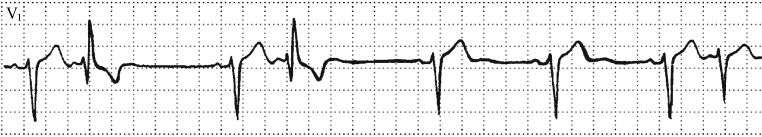
\includegraphics[width=3.21875in,height=2.30208in]{./images/Image00039.jpg}
\end{table}

\hypertarget{text00020.htmlux5cux23CHP1-7-2-1-1-4}{}
(4) 头痛的性质:

对头痛性质的了解十分重要。搏动性跳痛常为血管性头痛;发作性电击样剧痛为三叉神经痛的特征;咽后部发作性疼痛,可因吞咽动作诱发或加重者应考虑舌咽神经痛;紧箍样头痛多为肌紧张性头痛;眼、耳、鼻疾病所伴发者,大多数是胀痛或钝痛;神经症则是隐隐作痛,时轻时重。

\hypertarget{text00020.htmlux5cux23CHP1-7-2-1-1-5}{}
(5) 头痛的程度:

头痛的程度常不能反映病情的严重度,有时颅内占位性病变头痛并不严重而慢性焦虑症的头痛却表现剧烈难忍。一般而言,剧烈头痛常见于神经痛、偏头痛、蛛网膜下腔出血、脑膜炎等;中等度头痛,主要见于颅内占位性病变、慢性炎症等;轻度头痛,可见于神经症及某些邻近器官(耳、眼、鼻)病变。

\hypertarget{text00020.htmlux5cux23CHP1-7-2-1-1-6}{}
(6) 头痛发生的速度及影响因素:

急性突发性头痛,除多为血管性头痛外,尚有急性脑卒中(蛛网膜下腔出血、脑出血等)、急性感染性疾患。缓慢发生的头痛且进行性加重,并有颅内压增高表现者可能为颅内占位性病变,而无颅内压增高者可见于紧张性头痛。咳嗽、用力或头部转动,常使颅内压增高而头痛加剧;直立位可使肌紧张性头痛或腰穿后反应等加重,而丛集性头痛则减轻;压迫颞、额部动脉或颈总动脉可使血管性头痛减轻。根据头痛的发病方式和经过,对头痛进行鉴别诊断,见表\ref{tab7-2}。

\hypertarget{text00020.htmlux5cux23CHP1-7-2-1-1-7}{}
(7) 头痛的伴随症状:

头痛时常伴恶心、呕吐、面色苍白、出汗、心悸等自主神经症状,主要见于偏头痛;头痛严重并有进行性加剧的恶心、呕吐,常为颅内高压的征兆;体位变化时出现头痛加重或意识障碍,见于脑室内肿瘤、后颅凹或高颈段病变;伴有视力障碍及其他眼部征象(复视),呈短暂性发作者,多为偏头痛、椎-基底动脉供血不足;眼底视乳头水肿或出血,常为颅内压增高症或高血压性脑病。头痛伴精神症状(如淡漠或欣快)者应考虑额叶肿瘤的可能。由颅内损害引起的头痛常伴有神经功能缺失症状。

\hypertarget{text00020.htmlux5cux23CHP1-7-2-1-1-8}{}
(8) 其他病史:

尚需注意全身其他系统器官受损的病史,以及家族史、用药史、外伤史、手术史、月经及烟酒嗜好等。

\begin{table}[htbp]
\centering
\caption{头痛的发病方式和经过}
\label{tab7-2}
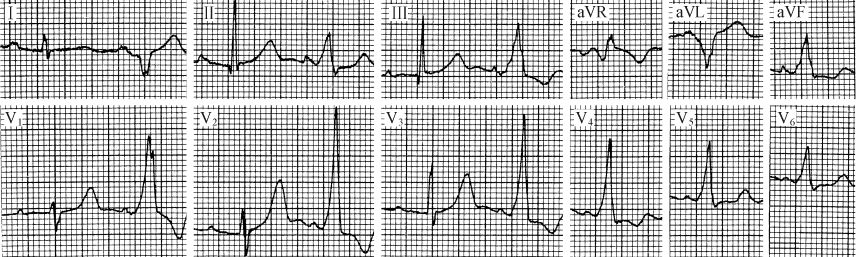
\includegraphics[width=3.22917in,height=4.33333in]{./images/Image00040.jpg}
\end{table}

\paragraph{体检}

全面详尽的体格检查尤其是神经系统和头颅五官的检查,有助于发现头痛的病变所在。

\hypertarget{text00020.htmlux5cux23CHP1-7-2-1-2-1}{}
(1) 内科检查:

许多内脏器官或系统的疾患可发生头痛,应按系统详细检查,大多可查出头痛的原因。如高血压、全身感染性疾病的发热或中暑、缺氧(如一氧化碳中毒),慢性肺部疾患的高碳酸血症,严重贫血或红细胞增多症,均可由于脑血流增加而致头痛;而毒素作用、酗酒,则可因血管扩张而致头痛。尚有代谢内分泌疾病的检查(甲亢、低血糖、嗜铬细胞瘤等)。

\hypertarget{text00020.htmlux5cux23CHP1-7-2-1-2-2}{}
(2) 五官检查:

头部邻近器官的疾病也是头痛常见的原因。如在眼部的视神经炎、儿童的屈光不正、青光眼、眼部表浅炎症(结膜炎、角膜炎、睑板腺炎、泪囊炎等)及眶部组织的炎症;在耳鼻咽喉方面有鼻炎、鼻窦炎、咽炎、中耳炎、鼻窦或鼻咽部肿瘤,另外颞颌关节病及严重的牙病也可引起头痛。

\hypertarget{text00020.htmlux5cux23CHP1-7-2-1-2-3}{}
(3) 神经系统检查:

全面的神经系统检查是非常重要的。

\hypertarget{text00020.htmlux5cux23CHP1-7-2-1-2-4}{}
(4) 精神检查:

有不少精神科疾病可伴有头痛,神经症是最常见的,而抑郁症的精神症状可被躯体症状所掩盖,尤其是隐匿性抑郁,常呈一些不典型的疼痛。

\paragraph{辅助检查}

应根据患者的具体情况和客观条件来选择性地应用。如做头颅X线检查、脑电图、CT扫描或MRI、腰穿脑脊液检查等,以及内科与五官科方面的检查。

头痛的临床检查方法见表\ref{tab7-3}。

\hypertarget{text00020.htmlux5cux23CHP1-7-2-2}{}
(二) 局限性病变抑或全身性病变

\paragraph{局限性病变}

包括颈部以上的局部病变引起的头痛,又可分为两大组:

\begin{table}[htbp]
\centering
\caption{头痛的临床检查方法}
\label{tab7-3}
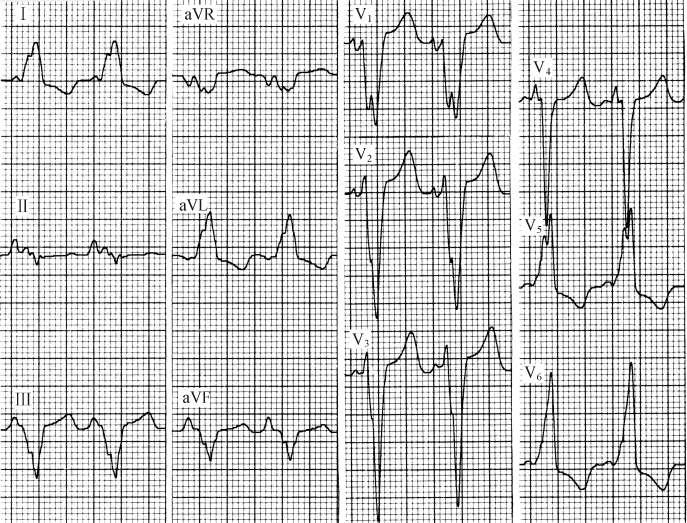
\includegraphics[width=3.25in,height=4.30208in]{./images/Image00041.jpg}
\end{table}

\hypertarget{text00020.htmlux5cux23CHP1-7-2-2-1-1}{}
(1) 颅内疾病:

此组疾病所致的头痛大都较严重,起病急,发展迅速。多数伴有恶心和(或)呕吐;部分尚有意识障碍或脑部和脑神经损害的表现,如抽搐、肢体瘫痪和瞳孔改变等。

\hypertarget{text00020.htmlux5cux23CHP1-7-2-2-1-2}{}
(2) 头颈部疾病:

此组疾病引起的头痛可轻可重,但很少逐渐加重。头痛的部位常与病灶一致或位于病灶附近,刺激病变部位可使疼痛加剧(如三叉神经痛等);但血管性头痛,压迫颞动脉则可使头痛减轻。头颈部疾病所致头痛的原发病灶明显,诊断不难。

\paragraph{全身性病变}

\hypertarget{text00020.htmlux5cux23CHP1-7-2-2-2-1}{}
(1) 全身性器质性病变:

引起急性头痛主要包括两大类疾病:一类是急性中毒。金属及化学物质如铅、锰、苯、酒精、一氧化碳等中毒时均可引起头痛。常为头部弥漫性跳痛,转动头部,头痛部位和性质无改变为此类头痛的重要特点。另一类是全身感染。多为急性传染病,头痛多在疾病的初期发生,也可出现在传染病的极期;无脑膜刺激征及神经系统定位征,脑脊液压力有时可增高,但生化及外观检查无异常。

\hypertarget{text00020.htmlux5cux23CHP1-7-2-2-2-2}{}
(2) 功能性病变:

多见于神经症患者,除头痛外,常伴有神经症的其他症状,如失眠、记忆力减退、注意力不集中、头昏、烦躁等,常因精神刺激而加重。患者一般情况好,临床检查无器质性病变存在。部分患者的头痛是由于服药后所引起(医源性头痛),主要是血管扩张剂等。应注意,功能性头痛必须在排除可能的器质性病变后才能确立。

\subsection{处理原则}

头痛的防治原则包括病因治疗、对症治疗和预防性治疗。对于病因明确的病例应尽早去除病因,如颅内感染应抗感染治疗,颅内高压者宜脱水降颅压等。任何头痛在急性发作时均应尽可能寻找潜在的病因进行治疗;对于病因不能立即纠正的继发性头痛及各种原发性头痛急性发作,可给予止痛等对症治疗以终止或减轻头痛症状。对慢性头痛呈反复发作者应给予适当的预防性治疗,以防头痛频繁发作。

\subsection{常见头痛的诊断与处理}

\hypertarget{text00020.htmlux5cux23CHP1-7-4-1}{}
(一) 偏头痛

偏头痛(migraine)是一种常见的慢性神经血管性疾患,是临床常见的原发性头痛,其特征是发作性、多为偏侧、中重度、搏动样头痛,一般持续4~72小时,可伴有恶心、呕吐,光、声刺激或日常活动均可加重头痛,安静环境、休息可缓解头痛。多起病于儿童和青春期,中青年期达发病高峰,女性多见,约50\%患者有家族史。精神紧张、过度劳累、气候骤变、强光刺激、烈日照射、低血糖、应用扩血管药物或利血平、食用高酪胺食物(如巧克力、乳酪、柑橘)及酒精类饮料,均可诱发偏头痛发作。

\paragraph{临床表现特点}

偏头痛有多种类型,但以以下两型常见:

\hypertarget{text00020.htmlux5cux23CHP1-7-4-1-1-1}{}
(1) 无先兆偏头痛(普通型偏头痛):

是最常见的偏头痛类型,约占80\%。临床表现为反复发作的一侧或双侧额颞部搏动性疼痛,常伴有恶心、呕吐、畏光、畏声、出汗、全身不适与头皮触痛等症状。通常在发作开始时仅为轻~中度的钝痛或不适感,数分钟至数小时后达到严重的搏动性痛或跳痛。有时疼痛放射至上颈部及肩部。部分女性患者发作常与月经有关,通常为经期前2天到经期的第3天之间发病,若90\%的发作与月经周期密切相关称月经期偏头痛。出现上述发作至少5次,除外颅内外各种器质性疾病后方可作出诊断。

\hypertarget{text00020.htmlux5cux23CHP1-7-4-1-1-2}{}
(2) 有先兆偏头痛(典型偏头痛):

约占偏头痛患者的10\%。一般在青春期发病,多有家族史,头痛发作前数小时至数日可有倦怠、注意力不集中和打哈欠等前驱症状。在头痛之前或头痛发生时,常以可逆的局灶性神经系统症状为先兆,表现为视觉、感觉、言语和运动的缺损或刺激症状。最常见为视觉先兆,常为双眼同向症状(homonymous
visual
symptoms),如视物模糊、暗点、闪光、亮点亮线或视物变形;其次为感觉先兆,感觉症状多呈面-手区域分布;言语和运动先兆少见。先兆症状一般在5~20分钟内逐渐形成,持续不超过60分钟;不同先兆可以接连出现。头痛在先兆同时或先兆后60分钟内发生,表现为一侧或双侧额颞部或眶后搏动性头痛,常伴有恶心、呕吐、畏光或畏声、苍白或出汗、多尿、易激怒、气味恐怖或疲劳感等,可见头面部水肿、颞动脉突出等。活动能使头痛加重,睡眠后可缓解头痛。头痛可持续4~72小时,消退后常有疲劳、倦怠、烦躁、无力和食欲差等,1~2日后常可好转。

有上述典型偏头痛症状,虽经治疗头痛时间持续在72小时以上(其间可能有短于4小时的缓解期)的称为偏头痛持续状态(status
migrainous)。

大多数偏头痛患者的预后良好,随年龄的增长症状可逐渐缓解,部分患者可在60~70岁时偏头痛不再发作。

\paragraph{治疗要点}

偏头痛的治疗目的为减轻或终止头痛发作,缓解伴发症状,预防头痛复发。

\hypertarget{text00020.htmlux5cux23CHP1-7-4-1-2-1}{}
(1) 发作期的治疗:

治疗药物包括非特异性止痛药如非甾体类抗炎药(NSAIDs)和阿片类药物,特异性药物如麦角类制剂(麦角胺1~2mg/次,日最大剂量6mg;双氢麦角胺肌肉注射1~2mg/次,日最大剂量4mg,或口服1~3mg/次,日最大剂量9mg)和曲普坦类药物,后者包括舒马曲普坦(皮下注射:6mg/次,日最大剂量12mg;口服25~100mg/次,日最大剂量300mg)、那拉曲普坦(口服2.5mg/次,日最大剂量5mg)、利扎曲普坦(口服5~10mg/次,日最大剂量30mg)、佐米曲普坦(口服2.5~5mg/次,日最大剂量10mg)和阿莫曲普坦(口服6.25~12.5mg/次,日最大剂量25mg)等。通常应在症状起始时立即服药。药物选择应根据头痛程度、伴随症状、既往用药情况等综合考虑,可采用阶梯法、分层选药,进行个体化治疗。①轻~中度头痛:单用NSAIDs如对乙酰氨基酚(口服0.3~0.6g/次,日最大剂量不超过2.0g)、萘普生(口服0.2~0.3g/次,每日2~3次)、布洛芬(口服0.2~0.4g/次,每日3~4次)等可有效,如无效再用偏头痛特异性治疗药物。阿片类制剂如哌替啶等,因有成瘾性,不推荐常规用于偏头痛的治疗,但对于有麦角类制剂或曲普坦类应用禁忌的病例,如合并心脏病、周围血管病或妊娠期偏头痛,则可给予哌替啶治疗以终止偏头痛急性发作。②中~重度头痛:可直接选用偏头痛特异性治疗药物以尽快改善症状,部分患者虽有严重头痛但以往发作对NSAIDs反应良好者,仍可选用NSAIDs。麦角类和曲普坦类药物不良反应包括恶心、呕吐、心悸、烦躁、焦虑、周围血管收缩,大量长期应用可引起高血压和肢体缺血性坏死。严重高血压、心脏病和孕妇患者均为禁忌。此外,应用过频,则会引起药物过量使用性头痛(medication-overuse
headache),因此,麦角类和曲普坦类药物每周用药不超过2~3天。③伴随症状:恶心呕吐可肌肉注射甲氧氯普胺10mg,严重呕吐者可用小剂量奋乃静、氯丙嗪。烦躁者可用地西泮10~20mg肌肉注射以促使患者镇静和入睡。

\hypertarget{text00020.htmlux5cux23CHP1-7-4-1-2-2}{}
(2) 预防性治疗:

适用于:①频繁发作,尤其是每周发作1次以上严重影响日常生活和工作的患者;②急性期治疗无效,或因副作用和禁忌证无法进行急性期治疗者;③可能导致永久性神经功能缺损的特殊变异型偏头痛,如偏瘫性偏头痛、基底型偏头痛或偏头痛性梗死等。常用药物有:①β受体阻滞剂:普萘洛尔(10~60mg/次,每天2次),美托洛尔(100~200mg/次,每天1次);②钙通道阻滞剂:氟桂利嗪(5~10mg,每日1次,睡前服用),维拉帕米(160~320mg/d);③抗癫痫药:丙戊酸钠(0.4~0.6g/次,每天2次),托吡酯(25~200mg/d),加巴喷丁(0.9~1.8g/d);④抗抑郁药:阿米替林(25~75mg睡前服用),丙米嗪和氟西汀等;⑤5-HT受体拮抗剂:苯噻啶(0.5~3mg/d)等。其中,普萘洛尔、阿米替林和丙戊酸钠三种在结构上无关的药物,是预防性治疗的支柱,一种药物无效可选用另一种药物。

\hypertarget{text00020.htmlux5cux23CHP1-7-4-2}{}
(二) 丛集性头痛

丛集性头痛(cluster
headache)是一种原发性神经血管性头痛。以男性多见,约为女性的3~4倍。头痛突然发生,无先兆症状,几乎于每日同一时间,常在晚上发作,使患者从睡眠中痛醒。头痛位于一侧眶周、眶上、眼球后和(或)颞部,呈尖锐、爆炸样、非搏动性剧痛。头痛达高峰时,患者常以手击头部、甚至以头撞墙,在室内外来回走动、十分烦躁、痛苦与不安。头痛持续15分钟~3小时不等。发作频度不一,从一日8次至隔日1次。疼痛时常伴有同侧颜面部自主神经功能症状,表现为结膜充血、流泪、流涕等副交感神经亢进症状,或瞳孔缩小和眼睑下垂等Horner征,较少伴有恶心、呕吐。头痛发作可连续数周至数月(常为2周~3个月),在此期间患者头痛呈一次接一次地成串发作,故名丛集性头痛。丛集发作期常在每年的春季和(或)秋季;丛集发作期后可有数月或数年的间歇期。在丛集期,饮酒或血管扩张药可诱发头痛发作,而在间歇期,两者均不会引起头痛发作。

根据中青年男性出现发作性单侧眶周、眶上和(或)颞部严重或极度严重的疼痛,可伴有同侧结膜充血、流泪、流涕、眼睑水肿、前额和面部出汗、瞳孔缩小、眼睑下垂等自主神经症状,发作时坐立不安、易激惹,并具有反复密集发作的特点,神经影像学排除引起头痛的颅内器质性疾患,可作出丛集性头痛的诊断。

本病急性期治疗方法有:①吸氧疗法:为头痛发作时首选的治疗措施。在发作剧烈时吸入纯氧(100\%氧气8~10L/min,10~20分钟)约使70\%患者终止发作。②利多卡因:用4\%~10\%利多卡因1ml经患侧鼻孔滴入,可使1/3的患者头痛缓解,机制是麻醉蝶腭神经节。③舒马曲普坦6mg皮下注射,或双氢麦角胺1~2mg肌肉注射等,可迅速缓解头痛。

本病预防性治疗药物包括维拉帕米、锂制剂和糖皮质激素等。维拉帕米240~320mg/d可有效预防本病发作,可在用药2~3周内发挥最大疗效。锂制剂适用于其他药物无效或有禁忌证者。糖皮质激素如泼尼松40~60mg/d,常可预防头痛的发作,第2周逐渐减量停药。其他药物有托吡酯、丙戊酸钠、苯噻啶、吲哚美辛等。

\hypertarget{text00020.htmlux5cux23CHP1-7-4-3}{}
(三) 紧张型头痛

紧张型头痛(tension-type headache)又称肌收缩性头痛(muscle contraction
headache),是双侧枕部或全头部紧缩性或压迫性头痛,约占头痛患者的40\%,是临床最常见的慢性头痛。主要由精神紧张及颅周肌肉张力增高引起。长期焦虑、紧张、抑郁或睡眠障碍,高强度的工作缺乏适当的放松及休息,以及某些单调工种使头、颈或肩胛带长期处于不良的姿势等均可为发病因素。头痛部位不定,可为双侧、单侧、全头部、颈项部、双侧枕部、双侧颞部等不同部位。通常呈持续性钝痛,像一条带子紧束头部或呈头周紧箍感、压迫感或沉重感。许多患者可伴有头昏、失眠、焦虑或抑郁等症状。有的患者也可出现恶心、畏光或畏声等症状。体检可发现疼痛部位肌肉触痛或压痛点,有时牵拉头发也有疼痛,颈肩部肌肉有僵硬感,捏压时肌肉感觉舒适。

根据患者的临床表现,排除颅颈部疾病如颈椎病、占位性病变和炎症性疾病等,通常可以确诊。

本病的许多治疗药物与偏头痛用药相同。对于焦虑、紧张或抑郁的患者应在精神上给予诱导和安慰,使其消除顾虑。对局限性的肌肉疼痛,如颈项肌和肩胛肌等可作按摩、针灸、理疗、局部封闭等治疗。急性发作期用对乙酰氨基酚、阿司匹林、非甾体抗炎药、麦角胺或双氢麦角胺等亦有效。对于频发性和慢性紧张型头痛,应采用预防性治疗,可选用阿米替林、丙米嗪或选择性5-羟色胺重摄取抑制剂(如舍曲林或氟西汀),或肌肉松弛剂如盐酸乙哌立松、巴氯芬等。失眠者可给予苯二氮{}
类如地西泮10~20mg/d口服。

\hypertarget{text00020.htmlux5cux23CHP1-7-4-4}{}
(四) 颅内压变化引起的头痛

\paragraph{颅内压增高所致的头痛}

脑瘤、硬膜下血肿、脑脓肿及其他占位性病变引起的头痛,在初期主要是因病变邻近疼痛敏感结构被牵拉、移位或因感觉神经直接受压所致。在后期是由于脑脊液循环通路被阻塞,导致颅内压增高,使远离病灶的对疼痛敏感结构被牵拉、扭曲和移位而引起头痛。初期的头痛常位于占位病变的同侧,在后期有颅内压增高时呈现为弥漫深在的持久性钝痛,晨起较重,在咳嗽、大便用力或打喷嚏时头痛加重。头痛程度一般不如偏头痛或颅内出血时那样严重,多数不影响睡眠。随着占位病变增大及颅内压增高,患者出现呕吐及视乳头水肿,最后因继发性视神经萎缩使视力减退或双目失明。治疗上除应用脱水剂降低颅内压外,根本措施是手术切除占位性病变。

良性颅内压增高征指有头痛和视乳头水肿等颅内压增高表现而无局灶性神经系统体征,抽搐、精神障碍,其脑室系统和脑脊液成分基本正常,颅内无占位性病变,预后较为良好的一种临床综合征。此症患者大都诉述有全面性的头痛,而并无脑部结构的移位,头痛可能是由于伴发的脑水肿牵引脑膜与脑血管的神经末梢所致。

\paragraph{低颅压性头痛}

低颅压性头痛(intracranial hypotension
headache)是脑脊液(CSF)压力降低(< 60mmH\textsubscript{2}
O)导致的头痛,多为体位性。患者常在直立后15分钟内出现头痛或头痛明显加剧,卧位后头痛缓解或消失。

低颅压性头痛包括自发性(特发性)和继发性两种。自发性病因不明,既往多认为可能与血管舒缩障碍引起CSF分泌减少或吸收增加有关;目前已证实多数自发性低颅压与自发性脑脊液漏有关。而导致自发性脑脊液漏可能与微小创伤和硬膜结构薄弱有关。部分病例有剧烈咳嗽、推举重物、剧烈体育活动等引起微小创伤的病史;部分病例可合并有结缔组织异常的其他疾病,如马方综合征(Marfan
syndrome)、常染色体显性遗传多囊肾、自发性视网膜脱离等。继发性可由多种原因引起,其中以硬膜或腰椎穿刺后低颅压性头痛最为多见,头颈部外伤及手术、脑室分流术、脊柱创伤或手术使CSF漏出增多,脱水、糖尿病酮症酸中毒、尿毒症、全身严重感染、脑膜脑炎、过度换气和低血压等使CSF生成减少。由于CSF量减少,压力降低,脑组织移位下沉等使颅内疼痛敏感组织被牵拉引起头痛。

本病可见于各种年龄,特发性多见于体弱女性,继发性无明显性别差异。头痛以双侧枕部或额部多见,也可为颞部或全头痛,但很少为单侧头痛,呈轻~中度钝痛或搏动性疼痛,缓慢加重,常伴恶心、呕吐、眩晕、耳鸣、颈僵和视物模糊等。头痛与体位有明显关系,立位时出现或加重,卧位时减轻或消失。脑组织下坠压迫脑神经也可引起视物模糊或视野缺损(视神经或视交叉受压)、面部麻木或疼痛(三叉神经受压)、面瘫或面肌痉挛(面神经受压)。

病因明确者应针对病因治疗,如控制感染、纠正脱水和糖尿病酮症酸中毒等。对手术或创伤后存在脑脊液瘘者可行瘘口修补术等。对症治疗包括头低位卧床休息,补液(2000~3000ml/d),穿紧身裤和束腹带,给予适量镇痛剂等。鞘内注射无菌生理盐水可使腰穿后头痛缓解。咖啡因可阻断腺苷受体,使颅内血管收缩,增加CSF压力和缓解头痛,可用苯甲酸钠咖啡因0.5g皮下或肌肉注射,或加入500~1000ml林格液中静脉滴注。硬膜外血贴疗法(epidural
blood
patching)是用自体血15~20ml缓慢注入腰或胸段硬膜外间隙,血液从注射点上下扩展数个椎间隙,可压迫硬膜囊和阻塞脑脊液漏出口,迅速缓解头痛,适用于腰穿后头痛和自发性低颅压性头痛,有效率97\%。腰穿时应选用口径细的穿刺针,术后去枕平卧至少6小时有利于预防头痛。

\hypertarget{text00020.htmlux5cux23CHP1-7-4-5}{}
(五) 脑血管病所致头痛

脑血管病所致头痛是急性头痛患者首先要甄别的,包括蛛网膜下腔出血、脑出血、缺血性卒中等。

\paragraph{蛛网膜下腔出血}

急性发作的头痛首先应考虑蛛网膜下腔出血的可能。典型症状为急性发作剧烈头痛,主诉为“刀劈样”、“爆炸样”头痛。70\%的头痛无定侧,可以为双额、顶、枕部或满头痛,30\%头痛偏向一侧,通常偏向动脉瘤所在侧。疼痛可放射至一侧或双侧眼部或颈部,可沿颈项向下放射,出现颈项强直,可持续数周至数月。可有意识丧失。也有一部分患者首发症状为精神错乱,惊厥发作,眩晕或脑神经(常为动眼神经瘫痪)障碍。腰穿脑脊液为均匀血性。患者如以往经常有阵发性头痛,此次头痛发作比较急剧,性质不同以往,也要考虑蛛网膜下腔出血。其处理参见第84章第4节“蛛网膜下腔出血”。

\paragraph{脑出血}

头痛常为首发症状,但往往迅速出现意识障碍与肢体偏瘫,结合血压突然升高的背景,诊断不难。

\paragraph{未破裂的脑动脉瘤与动静脉畸形}

一般在动脉瘤未破裂之前,头痛是不常见的。脑血管畸形头痛时常位于畸形同侧,如后交通动脉或颈内动脉瘤可以引起固定在同侧的眶、额部头痛。动脉瘤进一步扩张时可以出现眼肌瘫痪或对侧视野缺损,可以有局限性癫痫发作,对侧肢体偏瘫。DSA和(或)头颅MRI检查有助于诊断,治疗以手术为主。

\paragraph{缺血性脑卒中}

少数脑栓塞病例中有头痛症状,而在脑血栓形成中则头痛不常见。脑供血不足可致头痛,伴同感觉与运动障碍。头痛往往是搏动性的,可能是继发于颅外动脉的扩张。在椎-基底动脉或颈内动脉狭窄或闭塞的病例中,约1/3~1/2的患者有头痛,大都局限于枕部和颈部,或两额部;颈内动脉供血不足的头痛可以是同侧的或对侧的。

\paragraph{颞动脉炎}

颞动脉炎(temporal
arteritis)多见于中、老年人,头痛常位于头皮表浅部位以及颞部与眼眶周围部,也可较广泛地弥漫及额部与枕部,为一种强烈的搏动性和持续性疼痛,并且伴有在其他血管性头痛中所没有的烧灼感。平卧位或头低位头痛加剧,仰头或压迫颈总动脉时头痛减轻,咀嚼时头痛加重。咀嚼时出现头痛常为本病的首发症状。压迫眼球或眼球转动即出现眼窝部疼痛。头痛同时伴有面部肿胀、皮肤红肿、颞动脉明显扩张隆起呈蛇行状,搏动消失,触之有发硬肥厚感,压痛明显。部分病例视网膜动脉或脑动脉也可受累,可发生缺血性视神经炎而出现视力障碍。颞动脉炎多有发热、出汗、疲乏等全身症状,周围血象有白细胞增高,血沉增快。

本病如不加特殊治疗,通常在3~24个月内病情渐趋稳定或自愈,少数可持续几年。治疗主要用肾上腺皮质激素且疗效好,在激素开始治疗后数小时内体温即下降为正常,1~2天内局部疼痛和全身症状消失,食欲正常。头痛消失后激素可渐减量并维持用药数月,如停药后复发可重复再用。

\hypertarget{text00020.htmlux5cux23CHP1-7-4-6}{}
(六) 高血压性头痛

是一种非偏头痛型血管性头痛
。高血压病时约80\%出现不同程度头痛,且青壮年的高血压病头痛发生率高,其机制与动脉壁痛觉感受器受刺激有关。表现为头部沉重或间歇性钝痛、压迫感或搏动痛,或呈持续性全头或偏侧头痛,部位不固定,多在清晨或午前出现,在低头或屏气用力后头痛可加剧。恶性高血压伴高血压脑病或因嗜铬细胞瘤血压突然升高时均可出现剧烈的持续性头痛,常伴有恶心、呕吐、视力减退,视网膜出血或视乳头水肿。

高血压性头痛的治疗在于及时适度的降低血压。对伴有脑水肿者应及时应用脱水剂。

\hypertarget{text00020.htmlux5cux23CHP1-7-4-7}{}
(七) 颅脑外伤性头痛

急性和慢性头部外伤均可伴有头痛,常见的外伤后头痛有下列几种类型:①头皮裂伤或脑挫裂伤后瘢痕形成,刺激颅内外痛觉敏感结构而引起头痛。疼痛部位较局限,常伴局部皮肤痛觉过敏。②外伤后自主神经功能异常性头痛(dysautonomic
headache)是因颈前部受伤累及颈交感神经链,导致支配头颅的交感神经失去抑制而引起头痛。患者叙述一侧额颞区的发作性头痛,伴同侧瞳孔改变(先扩大后缩小),眼睑下垂及面部多汗。服用普萘洛尔(20mg,每天3次)对头痛有效。③外伤后因颈肌持续收缩而出现头痛,和紧张型头痛相似常有精神因素参与。④外伤后神经不稳定性头痛。常见于脑震荡后遗症,除头痛外尚有头晕、耳鸣、失眠、注意力不集中,记忆力衰退,精神萎靡不振或情绪易激动等症状。神经系统无器质性损害证据。

\hypertarget{text00020.htmlux5cux23CHP1-7-4-8}{}
(八) 五官疾病的头痛

眼源性头痛是指青光眼、虹膜炎、眼眶肿瘤、球后视神经炎、高度远视、眼外肌不平衡及用眼时间过长等原因引起球后或额颞区疼痛。急性乳突炎能引起耳后疼痛。病毒性膝状神经节带状疱疹所产生的疼痛常位于外耳道内或耳后,疼痛数日后出现带状疱疹及面瘫。鼻腔或鼻窦发炎时因黏膜充血水肿而引起鼻塞、流涕及牵涉性头痛。急性鼻窦炎时常引起眼球周围或额颞区头痛。因鼻窦内的脓性分泌物经过一夜睡眠后积聚增多,故患者清晨起床后头痛特别严重,待脓液排出后头痛明显减轻。X线检查有助于本病诊断。个别患者因鼻窦窦口被炎性分泌物或过敏性水肿阻塞,鼻窦内压力降低而形成“真空性头痛”(vacuum
headache)。牙病所致的头痛,多先有病牙部位疼痛,随后放射至同侧颞部,呈灼痛或跳痛,牙科检查可确诊。鼻腔肿瘤、颞下颌关节功能障碍(Costen综合征)及鼻咽癌均可引起头部牵涉痛。

\hypertarget{text00020.htmlux5cux23CHP1-7-4-9}{}
(九) 精神性头痛

神经症
、抑郁症等,经常出现头痛。其部位多不固定,多变,性质多样,呈钝痛、胀痛,易受外界或情绪影响,历时数周甚至数年。常伴睡眠及记忆、理解等精神方面的症状。

\hypertarget{text00020.htmlux5cux23CHP1-7-4-10}{}
(十) 神经痛

\paragraph{三叉神经痛(trigeminal neuralgia)}

是指三叉神经分布区内短暂的反复发作性剧痛。成年及老年人多见,40岁以上患者占70\%~80\%,女性多于男性。三叉神经痛可分为症状性和原发性,前者的病因为炎症(如疱疹病毒感染)、肿瘤(如半月神经节肿瘤)、动脉瘤及外伤等,后者系指病因未明者(可能因三叉神经脱髓鞘产生异位冲动或伪突触传递所致)。典型的原发性三叉神经痛通常有如下特点:①疼痛常局限于一侧,并以累及一支多见,少数患者可同时有二支或三支受累,且以上颌支(第2支)或下颌支(第3支)最常受累。②疼痛发作时表现为以面颊上下颌及舌部明显的剧烈电击样、刀割样、烧灼样或撕裂样疼痛,来去骤然,突发突止。疼痛由颌面或牙槽病灶开始,并沿该神经的支配区域放射,每次发作仅数秒钟至1~2分钟,间歇期正常,1天数次至1分钟多次。发作呈周期性,持续数周,可自行缓解数月或更长。随病程进展,缓解期日益缩短。③发作时可伴有同侧面部肌肉的反射性抽搐(故又称“痛性抽搐”),或有同侧面部潮红、流泪及流涎。④患者面部某个区域可能特别敏感,稍加触碰即引起疼痛发作,如上下唇、鼻翼外侧、舌侧缘、颊部等,该区域称之为“扳机点(触发点)”。发作期间面部的机械刺激,如说话、进食、洗脸、剃须、刷牙、打哈欠,甚至微风拂面皆可诱致疼痛发作,患者因而不敢大声说话、洗脸或进食,有的连口水也不敢咽下,严重影响患者生活,甚至全身营养状况不良,精神抑郁,有的产生消极情绪。

治疗主要有药物、封闭和手术治疗。药物治疗以卡马西平为首选,起始剂量0.1g口服,每天2~3次,最大剂量1.0g/d,有效维持量0.6~0.8g/d。如卡马西平无效可改用苯妥英钠0.1g口服,每天3次,如无效可每日增加0.05g,数日后加至0.6g/d。卡马西平或苯妥英钠单药治疗无效者两药合用可能有效。上述两药无效时可试用氯硝西泮(clonazepam)6~8mg/d口服。大剂量维生素B\textsubscript{12}
可缓解疼痛,剂量为1000~2000μg肌肉注射,每周2~3次,连用4~8周为一疗程。药物治疗无效者可试用无水乙醇或甘油封闭三叉神经分支或半月神经节,破坏感觉神经细胞,可获止痛效果,不良反应为注射区面部感觉缺失。经皮半月神经节射频电凝疗法也有较好疗效。三叉神经感觉根部分切除术,因止痛效果确切,仍是首选的手术治疗方法。而三叉神经显微血管减压术,止痛同时不产生感觉及运动障碍,是目前广泛应用的最安全有效的方法。

\paragraph{舌咽神经痛}

舌咽神经分布区的反复阵发性剧痛,不伴脑神经功能破坏表现的称舌咽神经痛(glossopharyngeal
neuralgia)。远比三叉神经痛少见。多数于中年起病,表现为口咽、喉或耳内的短暂发作性剧痛。每次持续数秒至1分钟,可因吞咽、咀嚼、讲话、咳嗽等触发。检查咽喉、舌根和扁桃体窝可有疼痛触发点。疼痛发作时可伴发咳嗽。个别患者发生昏厥,可能由于颈动脉窦神经过敏引起心脏停搏而造成。病程中可有自发缓解。神经系统检查无异常发现。将4\%可卡因或1\%丁卡因涂于患侧的口咽部,常可使疼痛缓解数小时。病因不明,有的可能是由于舌咽神经的脱髓鞘性病变引起,有的可能是由于局部的颅底血管压迫于舌咽神经所致。若疼痛持续,则本病需与鼻咽癌侵及颅底、耳咽管肿瘤、扁桃体肿瘤相鉴别。治疗与三叉神经痛相似。

\paragraph{枕神经痛}

枕神经痛(occipital
neuralgia)是枕大、枕小和耳大神经分布区疼痛的统称,三对神经来自C\textsubscript{2~3}
神经,分布于枕部。可因上段颈椎病、脊柱结核、骨关节炎、脊髓肿瘤、硬脊膜炎和转移瘤等所致,多为继发性神经损害;也可由上呼吸道感染或扁桃体炎引起,或病因不明。枕大神经分布于后枕部相当于两侧外耳道经头顶连线以后的部分;枕小神经主要分布于耳廓上部和枕外侧皮肤;耳大神经主要分布于耳廓下部前后面、腮腺表面和下颌角部皮肤。疼痛位于一侧枕部与颈部,呈阵发性刺痛或电击样痛,或持续性钝痛;患侧枕部头皮可有皮肤感觉过敏及局限性压痛点,可向头顶(枕大神经)、乳突部(枕小神经)或外耳(耳大神经)放射。枕大神经痛压痛点位于乳突与枕后粗隆间连线的中点;枕小神经痛的压痛点多位于该连线的外1/3处。部分患者在间歇期仍有钝痛。疼痛可为自发或因旋转尤其向对侧旋转而诱发,其他头颈部运动或咳嗽、喷嚏可使疼痛加重或诱发疼痛,故患者常不敢过分活动头部,或使头略向后仰并向患侧倾斜以缓解疼痛。除病因治疗外,可用止痛剂(卡马西平、苯妥英钠等)、神经营养剂(维生素B\textsubscript{1}
、B\textsubscript{12} 等)、局部封闭、理疗等对症治疗。


\hypertarget{text00021.htmlux5cux23CHP1-7-5}{}
参 考 文 献

1. 贾建平.神经病学.第6版,北京:人民卫生出版社,2008:158.

2. 头痛分类和诊断专家共识组
.头痛分类和诊断专家共识.中华神经科杂志,2007,40:439.

3. Schievink WI. Spontaneous spinal cerebrospinal fluid leaks and
intracranial hypotension. JAMA,2006,295:2286.

\protect\hypertarget{text00022.html}{}{}

\chapter{胸 痛}

胸痛是急诊室常见的患者就诊原因之一,临床上的胸痛不应仅是指解剖学胸部范围内的疼痛感受,而应包括任何原因所导致的解剖学胸部范围内的任何不适,同时也包括由于胸部疾患可能表现为其他部位的疼痛。由此可见导致胸痛的病因复杂,病情的严重程度相差很大。多数为良性经过的普通疾病,但其中有一部分则可能导致严重后果甚至危及生命。对于高危患者,症状发作后启动治疗越早,疗效越好,获益越多,任何延误都可能导致严重不良事件的发生,因此,急性胸痛患者的早期鉴别和危险分层对于识别高危患者并给予及时正确的处置具有重要意义。在临床急诊工作中,应首先确定就诊的急性胸痛患者是否患有急性心肌梗死、主动脉夹层、肺栓塞、气胸等,因为这些疾病若处理不及时,常危及生命。

\subsection{病因与发病机制}

\subsubsection{病因}

胸痛的主要病因大体上包括胸内结构病变、胸壁组织疾病、膈下脏器病变和功能性疾病等几个方面:

\paragraph{胸内结构病变}

\hypertarget{text00022.htmlux5cux23CHP1-8-1-1-1-1}{}
(1) 心源性胸痛:

心绞痛、急性心肌梗死、急性心包炎、主动脉夹层等。

\hypertarget{text00022.htmlux5cux23CHP1-8-1-1-1-2}{}
(2) 非心源性胸痛:

①大血管病变:主动脉瘤、肺梗死;②呼吸系统疾病:胸膜炎、自发性气胸等;③纵隔和膈肌的疾病:纵隔炎、纵隔脓肿、纵隔肿瘤和膈疝等;④食管疾病:反流性食管炎、食管破裂、食管裂孔疝等。

\paragraph{胸壁组织疾病}

带状疱疹、乳腺炎、皮下蜂窝组织炎、非化脓性肋软骨炎、肌炎、流行性肌炎、肋间神经炎、肋骨骨折等。

\paragraph{膈下脏器病变}

膈下脓肿、肝脓肿、脾梗死和肝癌破裂等。

\paragraph{功能性疾病}

心脏神经症。

\subsubsection{发病机制}

疼痛产生的机制:①各种化学或物理因素如缺氧、炎症、肌张力改变刺激肋间神经感觉纤维,脊髓后根传入纤维,支配气管、支气管及食管的迷走神经感觉纤维,膈神经的感觉纤维,支配心脏或主动脉感觉纤维等引起疼痛;②某一内脏与体表某一部位同受某些脊神经后根传入神经支配时,来自内脏的痛觉冲动传入大脑皮层区,除产生局部疼痛外,还可以出现相应体表的疼痛感觉------放射痛(又称牵涉痛)。

\subsection{诊断思路}

急性胸痛中包括了一组以胸痛为主要表现的疾病,其中危险性最高的分别是:急性心肌梗死、急性肺栓塞、主动脉夹层、张力性气胸及心包填塞。这些患者可能随时会发生死亡。急诊医生的任务是在众多表现为急性胸痛的患者中识别出这些高危的疾病并给予及时、适当的处理。这些高危的患者是否能够在急诊被及时准确地识别出来主要依靠:①急诊医生一定要时刻保持对这些疾病的警惕性;②急诊医生一定要掌握这些疾病主要的临床特征;③急诊科要有鉴别这些疾病的合理流程;④急诊科要能够提供必要的检查手段。

\subsubsection{临床特征}

首先在急诊处理急性胸痛的患者时,要利用有限的时间仔细询问病史和进行体格检查,这样能够确定下一步思考的正确方向。在询问病史时,要注意胸痛的部位、性质、缓解的因素,胸痛诱发和加重的因素,胸痛是否放射,胸痛的伴随症状和既往病史等。这些特征中往往隐含着具有诊断和鉴别诊断意义的线索,因此这些特征是医生接诊急性胸痛患者时需要重点询问的内容,相当部分的胸痛患者单纯依靠详细的病史询问就可以基本诊断。

\paragraph{发病年龄}

青壮年胸痛,应注意自发性气胸、心肌炎、心肌病、风湿性心瓣膜病,40岁以上患者应注意心绞痛、心肌梗死与肺癌。

\paragraph{胸痛部位}

包括疼痛部位及其放射部位。心绞痛与心肌梗死的疼痛常位于胸骨后或心前区,且放射到左肩和左上臂内侧。夹层动脉瘤疼痛位于胸背部,向下放射至下腹、腰部与两侧腹股沟和下肢。食管疾患、膈疝、纵隔肿瘤的疼痛也位于胸骨后。胸膜炎所致的胸痛常在胸廓的下侧部或前部。带状疱疹是成簇水疱沿一侧肋间神经分布伴剧痛,疱疹不越过体表中线。胸壁疾病特点为疼痛部位局限,局部有压痛。炎症性疾病,尚伴有局部红、肿、热表现。肝胆疾病或膈下脓肿可引起右下胸痛。

\paragraph{持续时间}

心绞痛发作时间短暂,持续数分钟,而心肌梗死疼痛持续时间很长且不易缓解。炎症、肿瘤、栓塞或梗死所致疼痛呈持续性。平滑肌痉挛或血管狭窄缺血所致疼痛为阵发性。

\paragraph{疼痛性质}

胸痛的程度可表现为剧烈的疼痛到轻微的隐痛,疼痛性质也多种多样。如带状疱疹呈刀割样痛或灼痛,剧烈难忍;肌痛呈酸痛;骨痛呈酸痛或锥痛。心绞痛常呈压榨样痛并伴有压迫感或窒息感;主动脉夹层动脉瘤常有突然出现的剧烈的撕裂痛。膈疝呈灼痛或膨胀感。早期肺癌可仅有胸部的钝痛或隐痛。食管疾病多表现为持续性隐痛或烧灼痛。

\paragraph{伴随症状}

气管、支气管疾病所致胸痛常伴有咳嗽、咳痰;食管疾病所致胸痛常伴有吞咽困难或咽下疼痛;肺梗死、原发性肺癌的胸痛常伴有小量咯血或痰中带血。

\paragraph{影响疼痛因素}

包括发生诱因、加重与缓解因素。胸膜炎、自发性气胸、心包炎所致胸痛常在深吸气及咳嗽时加重,停止呼吸运动则疼痛减轻或消失。劳累、体力活动、精神紧张,可诱发心绞痛发作,休息、含服硝酸酯类药物可使心绞痛缓解,而对心肌梗死疼痛则无效。反流性食管炎的胸骨后灼痛,饱餐后出现,仰卧或俯卧位加重,服用抗酸剂和促动力药后可减轻或消失。

\subsubsection{必要的体格检查}

对于急性胸痛患者,一般不可能进行全面、系统的体格检查,要求5分钟内完全必要的体格检查。因为大多数情况下病情不允许医生有充分的时间这样做,因此重要的是要有针对性,有目的地根据患者的病史特征和临床思维分析进行一些重点体查。

首先要注意生命征,包括血压、脉搏、呼吸、体温。发现患者血压<
90/60mmHg,心率> 100次/分钟,应立即启动稳定生命征治疗。

怀疑主动脉夹层对比双侧桡动脉、股动脉和足背动脉搏动,有怀疑应测四肢血压。

观察胸部表面皮肤有无局限性红肿、瘀斑和出血点及疱疹等;胸腹式呼吸协调性、呼吸形式和快慢深浅;双侧胸部对称性。胸膜炎、胸腹部外伤、膈下脓肿、单纯疱疹等疾病常有上述异常变化。触诊检查局部肿块、液波感、压痛和胸廓的呼吸动度。

注意胸壁感染、气胸、血胸、肋骨骨折等征象。女性乳腺炎也有以胸痛主诉就诊,注意鉴别。

听诊需了解双侧呼吸音对比、胸膜和心包摩擦音、肺干湿性啰音、哮鸣音、异常音和杂音等,这对鉴别心脏和肺部疾病有帮助。

怀疑肺栓塞的患者要注意检查下肢有无肿胀,是否有下肢深静脉血栓形成的证据。

\subsubsection{必要的辅助检查}

对胸痛的诊断,除需仔细了解病史、查体外,一些常规的辅助检查,如心电图(ECG)、心肌损伤标志物及影像学检查也十分重要,这对筛查潜在的高危胸痛患者有参考价值。

\paragraph{实验室检查}

血常规检查和凝血功能对判断有无感染和出凝血异常的存在必不可少。初始的ECG有助于确定中~高危的ACS患者,肌钙蛋白和心肌酶学是确诊是否存在心肌损害的重要手段,应用肌钙蛋白有助于确定是否需要早期血运重建,是ACS危险分层的重要工具;D-二聚体对急性肺栓塞的诊断有重要意义;动脉血气分析有助于了解肺功能情况。

\paragraph{心肌损伤标记物在胸痛患者中的应用价值}

心肌损伤标志物的测定能检出或除外心肌坏死,最常应用的生化标志物有肌钙蛋白T(TnT)和肌钙蛋白I(Tn
I)、肌红蛋白和肌酸激酶MB同工酶(CK-MB)。在急性胸痛的早期约3~6小时,肌红蛋白检测对除外心肌梗死的可能性很有价值,在症状发作7小时后,肌钙蛋白与CK-MB有较高的阴性预测性,Tn
I或TnT对诊断AMI的特异性与敏感性均较高。心肌损伤标记物浓度与心肌损害范围呈正相关。约30\%的非ST段升高的ACS患者cTn
I或cTnT升高,可能为非Q波心肌梗死而属高危患者,即使CK-MB正常,死亡危险性也增加。肌钙蛋白水平越高,危险性越高。

\paragraph{心电图}

ECG是胸痛患者应用广泛的检查方法。异常的心电图包括ST段升高、ST段下降和T波低平或倒置。入院时ECG有ST段升高的患者早期死亡率最高,ST段下降患者的死亡率中等,T波倒置最低。ST段升高是急性心肌梗死最敏感和最特异的ECG标志。新出现ST段升高的患者80\%~90\%为急性心肌梗死。约90\%的ECG有新出现的Q波为急性心肌梗死。ST段下降提示心肌缺血,但是其诊断进展性心肌梗死的可靠性差,仅约50\%的患者最终确诊为急性心肌梗死。对称性T波倒置的特异性较差,心肌缺血、心肌炎和肺栓塞在内的多种疾病都可以出现这种改变,约1/3的患者可能存在心肌梗死。有1/3左右的急性胸痛患者ECG正常,对这些患者动态观察心电图的变化很重要。在发病早期,很多急性心肌梗死最初的心电图无异常,随着时间的延长才表现为急性心肌梗死典型的ST段升高的ECG表现,若未对患者进行动态观察,常易忽略而漏诊。

目前建议在胸痛患者来诊10分钟内应进行ECG检查,10分钟内做出判定,ST段升高的患者一旦确定需立即进行再灌注治疗;ECG有缺血性表现的患者,按不稳定性心绞痛或非ST段升高的急性心肌梗死处理;ECG正常或有非特异性改变,应结合病史和生化标志物等综合判断。

\paragraph{影像学检查}

X线胸部透视与摄片,对于鉴别肺部疾病、肋骨、胸骨骨折,心脏各房室大小有帮助;CT扫描是一项对临床有较大帮助的检查,可以发现X线不能显示的病变,帮助临床诊断肺栓塞、主动脉瘤、夹层动脉瘤。心血管造影,尤其血管数字减影(DSA),可清楚显示主动脉瘤、主动脉夹层、室壁瘤的部位、大小、形态等情况;冠状动脉造影,可明确心肌梗死的部位和严重程度,是诊断心肌梗死的“金标准”;超声心动图实时显示心脏结构和动态以及心包积液。B超对膈下和肝脓肿、胆道情况以及包裹性胸水定位有意义。

\paragraph{放射性核素扫描}

对肺梗死、肺内占位病变、心肌梗死或局限性室壁瘤的诊断有帮助。

\paragraph{彩色多普勒超声}

对急性心肌梗死和急性大动脉夹层动脉瘤诊断的意义较大。彩超和多普勒可用于大动脉夹层的检查,但其具有一定的局限性。彩超仅能看到升主动脉和腹部、髂部的血管。主要的征象是主动脉明显增宽,主动脉壁分离形成的真腔与假腔,有时还可见内膜的裂口。超声还可用于鉴别胆石症、脾梗死、胰腺炎等一些膈下疾病。急性心肌梗死时二维超声心动图可见梗死的部位室壁运动低下、运动消失或反常运动。超声对急性肺栓塞的诊断帮助不大。超声对自发性气胸的诊断没有帮助。

\paragraph{胸痛患者辅助检查的顺序}

决定检查的顺序时要根据:危险性最大、最需要首先排除的疾病是什么?最能明确诊断的检查是什么?最方便、最及时的检查是什么?对于所有胸痛的患者,首先是要进行详细的体格检查,尤其是要注意生命体征,其次才是借助仪器的检查。有些疾病经过仔细的体格检查就能够发现特征性的表现,如剧烈胸痛者发现脉搏不对称及血管杂音强烈提示大动脉夹层等。切忌一切依赖仪器。对于一个急性胸痛的患者,辅助检查应该按照以下顺序进行为宜:

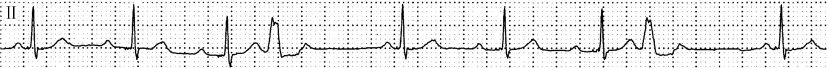
\includegraphics[width=3.09375in,height=0.94792in]{./images/Image00043.jpg}

\subsection{急诊处理原则和流程}

急性胸痛的急诊处理原则是:一是快速识别高危患者,以迅速进入快速救治绿色通道;剔除那些几乎没有或没有威胁生命疾病的患者;二是对不能明确诊断的患者应常规留院观察病情的演变,严防患者院外发生严重危及生命的事件。

1.首先判断病情严重性
,对生命征不稳定的患者,应立即开始稳定生命征的治疗;同时开始下一步处理;

2.对于生命征稳定的患者,首先获取病史和体征;

3.进行针对性的辅助检查;

4.在上述程序完成后能够明确病因的患者立即开始有针对性地病因治疗;

5.对不能明确病因的患者,建议留院观察,每隔30分钟复查一次心电图,每隔2小时复查心肌损伤标志物。心电图连续3次无变化,心肌损伤标志物连续2次无异常者在6~12小时后可予以出院。具体处理流程见图\ref{fig8-1}。

\begin{figure}[!htbp]
 \centering
 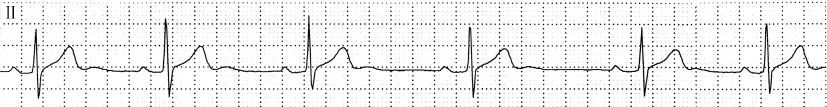
\includegraphics[width=4.69792in,height=5.41667in]{./images/Image00044.jpg}
 \captionsetup{justification=centering}
 \caption{胸痛的处理流程图}
 \label{fig8-1}
  \end{figure} 

\hypertarget{text00023.htmlux5cux23CHP1-8-4}{}
参 考 文 献

1. O'Connor R E,Bossaert L,Arntz H R,et al. Acute Coronary
Syndromes:2010 International Consensus on Cardiopulmonary Resuscitation
and Emergency Cardiovascular Care Science With Treatment
Recommendations. Circulation,2010,122: S422-S465.

2. Braunwald E,Antman E M,Beasley J W,et al. ACC/AHA Guideline Update
for the Management of Patients With Unstable Angina and Non-ST-Segment
Elevation Myocardial Infarction---2002:Summary Article:A Report of the
American College of Cardiology/American Heart Association Task Force on
Practice Guidelines(Committee on the Management of Patients With
Unstable Angina).Circulation,2002,106:1893-1900.

3. 罗学宏.急诊医学.北京:高等教育出版社,2008.74-78.

\protect\hypertarget{text00024.html}{}{}

\chapter{咯 血}

咯血(hemoptysis)是指喉腔、气管、支气管和肺组织出血,由咳嗽动作经口腔排出。咯血的临床过程难以预料,有时,初始仅少量痰中带血,却可以是大量的致命性咯血的先兆。大咯血引起失血性休克而致死的较少见,更常见的是大量的血淹溺肺泡,阻塞气道,因窒息和顽固性低氧血症而导致患者死亡。

咯血量可因病因和病变性质的不同而有差异,与病变的严重程度也不完全一致。临床上多根据咯血量将其分为少量咯血:24小时内咯血量≤100ml,包括痰中带血;中等量咯血:24小时内咯血量100~500ml;大咯血:24小时内咯血量>
500ml或一次咯血量≥200ml。大咯血约占全部咯血患者的1\%~4\%,但其死亡率高达80\%以上。

大咯血致死的危险与咯血量、出血速度、肺内潴留的血量以及患者基础肺功能储备相关,而与咯血的病因无关。年老体弱或久病无力者咳嗽乏力、基础肺功能差,即使几口血痰也可窒息致死。

\subsection{病因与发病机制}

\subsubsection{病因}

咯血的病因很多(表\ref{tab9-1}),但以肺结核、支气管扩张症、肺癌和肺炎等4种疾病多见。

尽管当今的检查手段有了长足的发展,对咯血患者采用了各种检查方法,但仍可有5\%~15\%的患者咯血原因不明,这类患者称隐匿性咯血(occult
hemoptysis)。部分隐匿性咯血可能由于气管、支气管的非特异性溃疡、静脉曲张、早期腺瘤、支气管小结石及轻微支气管扩张等病变引起。

\subsubsection{发病机制}

许多肺内外疾病和全身性疾病均可引起咯血,但咯血的机制有所不同。一般说来,炎症或肿瘤多导致病灶局部的毛细血管破坏,如不侵蚀支气管动脉,则咯血量一般较小。病变若侵蚀小动脉、小动静脉瘤或黏膜下静脉破裂则常常出现中等量或大咯血,而全身性疾病或严重而广泛的毛细血管炎症导致的咯血大多为中等量。小到中等量咯血大多可以自行终止,所以咯血很少引起失血性休克。

\begin{table}[htbp]
\centering
\caption{咯血的常见病因}
\label{tab9-1}
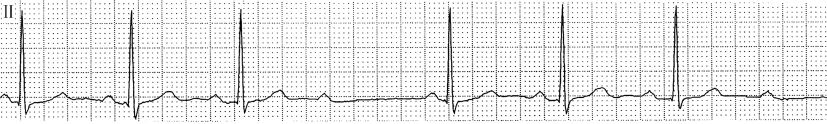
\includegraphics[width=6.59375in,height=3.875in]{./images/Image00045.jpg}
\end{table}

\paragraph{气管、支气管疾病}

各种病原微生物如细菌、病毒、支原体、寄生虫以及肿瘤、各种粉尘、异物、结石等,均可侵蚀气道邻近血管或肺泡毛细血管导致咯血。支气管扩张导致的咯血常见,炎性病变侵蚀血管壁,使血管弹性纤维遭到破坏或在支气管壁下形成假性动脉瘤,当用力咳嗽时血管破裂导致大咯血;癌组织可直接侵蚀血管壁破裂导致咯血,少到痰中带血,多到大咯血窒息均可发生。

\paragraph{肺部疾病}

许多肺部病变可直接侵蚀血管致使破裂出血或肺毛细血管床广泛损伤出血。大咯血最常见于肺结核(尤见于空洞性肺结核)、急性肺脓肿、癌性坏死及空洞形成、肺囊肿继发感染等,其穿行的支气管动脉或肺动脉受蚀,或动脉壁肌纤维破坏形成假性动脉瘤因咳嗽而破裂出血。此类咯血可因血凝块暂时充填空洞而压迫血管暂停出血,但也可因血凝块自溶而再次出现咯血。慢性肺脓肿多引起小量咯血,偶有大咯血发生。

\paragraph{肺血管病变或先天性病变}

支气管动脉-肺动脉瘘是由于肺动脉因体循环压力,形成动脉瘤,破溃出血。肺动脉栓塞、多动脉炎、白塞病的病变基础多为栓塞性动脉炎或动脉瘤样扩张。夹层动脉瘤或梅毒性动脉瘤,偶与支气管动脉相通,可造成致命性大咯血。原发性肺动脉高压可因肺动脉远端阻力加大,肺动脉与肺毛细血管形成侧支循环,当血管破裂时引起咯血。偶见于先天性肺动-静脉瘘,先天性毛细血管扩张症引起的咯血。

\paragraph{心血管疾病}

最常见的原因是二尖瓣狭窄和冠心病、心肌病等疾病导致的急性左心功能不全。左房血流受阻造成左房压力高,心脏前负荷增加,肺毛细血管及肺静脉压力升高,导致肺血管扩张,肺处于淤血状态,可引起肺水肿,并导致支气管黏膜下小静脉曲张,常自发或在炎症诱发下引起小静脉及毛细血管破裂,导致大咯血。

\paragraph{全身性疾病}

脓毒症、肾出血-出血热综合征、出血型钩端螺旋体病等急性全身感染性疾病、血液病和某些自身免疫性疾病如大动脉炎、白塞病、系统性红斑狼疮、肺出血-肾炎综合征(Goodpasture
syndrome)、子宫内膜异位症等病变,使肺微血管和毛细血管受损,血管内皮细胞功能障碍,血管脆性增加以及血小板减少或功能障碍导致出血。此类咯血多为弥漫性肺泡出血。

\paragraph{出凝血机制障碍}

包括血液系统疾病及DIC所致的咯血,多为全身多脏器出血的一部分。多见于全身性疾病导致的血小板减少和(或)功能障碍、凝血因子缺乏和(或)功能异常。此类咯血为原发病的继发性改变,罕见情况下咯血可能为首发症状。

\subsection{诊断思路}

多数咯血患者为突然起病,尤其第一次见到咯出鲜血,精神高度紧张,甚至有恐惧感,往往不能正确的诉说相关的症状及所见到血液的性状。因此,明确出血部位和出血原因显得尤为重要。

\paragraph{确定出血部位}

口腔、鼻腔、咽喉部以及消化道出血有时可误认为咯血,特别是后鼻道出血多流入口腔或食管出血未经胃酸作用直接呕出时,有时会出现刺激性咳嗽而导致对出血部位判断的错误,即所谓的“假性咯血”(pseudo-hemoptysis)。对首次从口腔内咳或呕血者,在不能判断出血部位的情况下,应仔细寻找出血部位。对可疑鼻咽部出血者,应迅速邀请专科会诊以明确诊断。详细询问病史和仔细的体格检查多能明确。呕血在大多数情况下诊断并无困难,在临床上可依据临床表现、体格检查、辅助检查和实验室检查予以区别。

\paragraph{临床表现特点}

除有原发病症状与体征外,大多数情况下,患者咯血前常有喉部痒感,血呈弱碱性,色鲜红,呈泡沫状,多混有痰液,咯血后数天内仍可咳出血痰。常见咯血病因的临床表现特点见表\ref{tab9-2}。

\begin{table}[htbp]
\centering
\caption{常见咯血原因的临床表现特点}
\label{tab9-2}
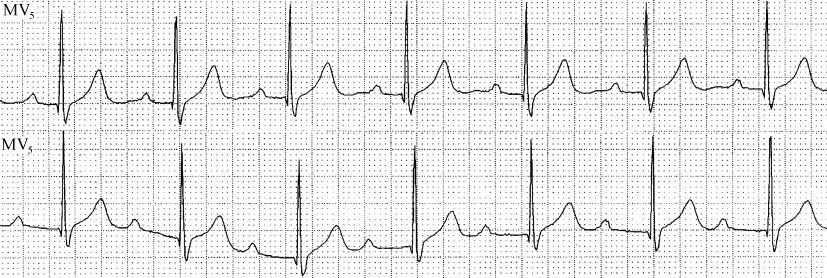
\includegraphics[width=3.26042in,height=2.38542in]{./images/Image00046.jpg}
\end{table}

大量咯血可引起急性出血性休克而出现面色苍白、冷汗、四肢湿凉,血管充盈度下降,血压降低等表现。因血凝块阻塞气道出现窒息的特征为咯血量突然减少或停止,同时出现胸闷、双手抓胸、喉头异常作响、继而烦躁不安、表情呆滞或恐惧、目瞪口张、全身发绀、呼吸变浅、速率加快,大小便失禁,肺部检查可见一侧或双侧呼吸音消失,进而呼吸突然停止。其他还包括肺不张和肺部继发感染等并发症的临床表现。

\paragraph{咯血与呕血的鉴别}

大量呕血时,鲜红色血液可从口腔及鼻腔涌出,或大咯血时部分血液咽下,复又呕出,致使咯血与呕血不宜鉴别。正确的鉴别诊断有助于采取恰当的治疗措施。咯血与呕血的鉴别见表\ref{tab9-3}。

\begin{table}[htbp]
\centering
\caption{咯血与呕血的鉴别}
\label{tab9-3}
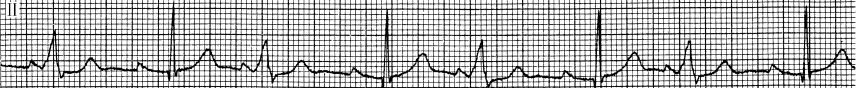
\includegraphics[width=3.26042in,height=2.05208in]{./images/Image00047.jpg}
\end{table}

\paragraph{辅助检查与实验室检查}

\hypertarget{text00024.htmlux5cux23CHP1-9-2-4-1}{}
(1) 影像学检查:

胸部X线可初步判断胸部病变的性质和部位。胸部CT检查有助于支气管、肺部和胸腔疾病的病因诊断。尤其是高分辨CT(HRCT)可显示次级肺小叶为基本单位的细微结构,可明确病变的性质及范围,基本上已代替支气管造影。HRCT及核素扫描可明确心肺血管病变及占位性病变。必要时可作支气管动脉造影,但一般仅用于介入治疗前对出血部位的精准定位。

\hypertarget{text00024.htmlux5cux23CHP1-9-2-4-2}{}
(2) 超声与心电图检查:

心脏彩色多普勒与心电图检查对心脏病变诊断有帮助,可发现各种类型心脏结构改变、心律失常、ST-T段等改变。腹部B超有助于了解肝、脾、腹水、腹腔肿物等情况。

\hypertarget{text00024.htmlux5cux23CHP1-9-2-4-3}{}
(3) 血常规及生化检查:

可见白细胞总数增加,以中性粒细胞增加为主时提示感染存在。出血较多时可见红细胞和血红蛋白含量下降,血小板可正常。凝血功能、肝功能、肾功能等异常均能对其原发病提供参考。血气分析有助于发现病情较重患者的低氧血症。

\hypertarget{text00024.htmlux5cux23CHP1-9-2-4-4}{}
(4) 痰液检查:

细菌、真菌和细胞学检查有助于原发病的诊断和治疗。

\hypertarget{text00024.htmlux5cux23CHP1-9-2-4-5}{}
(5) 特异性检查:

如结核菌素试验、免疫学检查有时会对结核病、结缔组织疾病的诊断具有重要参考价值。

\hypertarget{text00024.htmlux5cux23CHP1-9-2-4-6}{}
(6) 纤维支气管镜检查:

可发现部分患者的出血部位和性质,并可在镜下止血,同时还可进行局部灌洗、标本取样做病原学和细胞学检查。

\hypertarget{text00024.htmlux5cux23CHP1-9-2-4-7}{}
(7) 动脉造影:

支气管动脉造影可显示区域性支气管动脉异常,确定出血部位,是决定进行栓塞治疗的主要依据。肺动脉造影对来自肺动脉的大咯血,尤其是支气管动脉栓塞后继续出血者适用。对空洞性肺结核或其他肺化脓性疾病、疑Rasmussen动脉瘤或肺动静脉瘘所致的咯血,选择性支气管动脉及肺动脉造影应同时进行,若病变波及双重动脉系统,则可以同时作栓塞治疗,以免术后继续出血。

\paragraph{常见疾病鉴别诊断}

通过询问与咯血相关的病史、诱因、咯血量和伴随症状以及详细的体格检查多能寻找到原发疾病的线索。体格检查应注意有无肺部啰音、皮肤黏膜有无出血、淋巴结是否肿大、有无肝脾肿大、心脏杂音及体重减轻等。出血部位的判断可根据肺部体征及X线检查确定。

\hypertarget{text00024.htmlux5cux23CHP1-9-2-5-1}{}
(1) 支气管扩张:

缓慢起病,反复咳嗽伴脓痰和(或)量不等的咯血。既往多有麻疹、肺炎或免疫缺陷等病史。部分患者咯血为唯一症状,即所谓的“干性支气管扩张”。部分患者表现为反复发生的同一肺段感染,并迁延不愈,查体可闻及患侧固定而持久的湿啰音,可见杵状指(趾)等。胸部X线摄片或CT均可明确诊断。

\hypertarget{text00024.htmlux5cux23CHP1-9-2-5-2}{}
(2) 肺结核:

活动期多有午后低热、乏力、食欲减退、盗汗等结核中毒症状,部分可有不规则性高热。痰检或培养结核分枝杆菌阳性。查体可见结核面容、消瘦,局部湿啰音等。胸部X线摄片或CT表现多种形态,如局部渗出、增殖、纤维化、干酪性病变、钙化或空洞形成,以肺上叶尖后段及后基底段多见,可伴有胸腔积液、胸膜肥厚与粘连。聚合酶链反应(PCR)及结核菌素纯蛋白衍生物实验(purified
protein
derivative,PPD)有助于确定诊断,但后者不能区分是自然感染还是卡介苗免疫反应。

\hypertarget{text00024.htmlux5cux23CHP1-9-2-5-3}{}
(3) 肺癌:

持续出现咳嗽、咳痰,不明原因体重下降,近期痰中带血,反复出现。晚期可出现与呼吸运动有关联的胸痛及血性胸腔积液。查体可见气促、肺局限性喘鸣音、呼吸音增强或单侧胸腔积液、转移性骨压痛、淋巴结肿大(以颈部、腋窝为主,右锁骨上窝淋巴结肿大具有特殊诊断意义)等。胸部X线摄片或CT有助于诊断,痰液细胞学及活检可明确诊断。

\hypertarget{text00024.htmlux5cux23CHP1-9-2-5-4}{}
(4) 肺脓肿:

急性起病,多有劳累、受凉等病史。高热伴有不同程度的咯血。发病两周左右突然咳出大量脓痰及坏死组织,痰咳出后,体温下降。查体可发现局部湿啰音,偶可闻及空瓮音,宜可见杵状指(趾)。胸部X线摄片或CT和痰液细菌培养阳性多能明确诊断。

\hypertarget{text00024.htmlux5cux23CHP1-9-2-5-5}{}
(5) 风湿性二尖瓣狭窄:

有风湿性心脏病史。常在感冒、活动后出现呼吸困难,严重时不能平卧,常出现急性左心功能不全表现,伴以咳出大量粉红色泡沫样痰。小量咯血多见,偶见大量咯血。查体可见“二尖瓣面容”,心尖部听诊可及第一心音亢进、开瓣音、舒张中晚期隆隆样杂音、肺动脉瓣区第二心音亢进等,部分患者可摸到舒张期震颤。心脏多普勒超声检查可明确诊断。

\hypertarget{text00024.htmlux5cux23CHP1-9-2-5-6}{}
(6) 急性肺梗死:

有长期卧床、骨折、静脉炎或心房纤颤等病史。突然出现胸痛、胸闷、心悸、烦躁、冷汗,甚至晕厥,以小~中等量咯血多见。查体可见呼吸加快,肺局部叩诊浊音、呼吸音减弱及干湿性啰音。严重者可见急性右心衰表现,如心率加快、肺动脉瓣第二心音亢进、三尖瓣区可闻及收缩期杂音,可伴心律失常。血压下降,颈静脉怒张,肝脏增大、肝颈征阳性等。D-二聚体阳性及胸部X线摄片或CT有助于诊断。

\hypertarget{text00024.htmlux5cux23CHP1-9-2-5-7}{}
(7) 其他咯血的病因诊断:

其他一些肺部或全身性病变引起的咯血,根据发病特点和辅助诊断特征,大多数诊断并不是很困难。重要的是要想到一些引起咯血的少见原因,如肺血管畸形、血液病、结缔组织病、肺肉芽肿症、遗传性毛细血管扩张症、肺出血-肾炎综合征、经期性咯血等。弥漫性肺泡出血诊断的最好方法是通过灌洗获得肺泡巨噬细胞中的含铁血黄素来确定。目前ICU中出现的咯血日益增多,大多数为弥漫性肺泡出血,少部分为设备使用或操作不当导致的大咯血,应引起足够重视。

咯血病因诊断流程见图\ref{fig9-1}。

\subsection{病情评估}

咯血患者出现下列情况表明病情危重:咯血量较大,一次超过200ml,反复发作,一般止血措施不能控制;精神高度紧张或恐惧,呼吸困难、胸闷,双手无目的抓挠喉或胸部,表明出现窒息先兆;短期内即出现失血性休克表现;胸部X线片(或CT扫描)提示空洞或可疑病变侵及小动脉及假性动脉瘤破裂。

\subsection{处理原则}

咯血的急诊治疗取决于速度与量。大咯血抢救的重点在于迅速有效止血,保持呼吸道通畅,防治窒息及其他并发症,并同时进行病因、对症治疗。

\subsubsection{窒息的紧急处理}

咯血窒息是导致患者死亡的主要原因,应及早识别和抢救。窒息抢救的重点是保持呼吸道通畅和纠正缺氧。

\begin{figure}[!htbp]
 \centering
 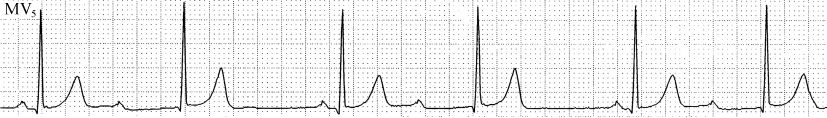
\includegraphics[width=4.55208in,height=5.47917in]{./images/Image00048.jpg}
 \captionsetup{justification=centering}
 \caption{咯血病因诊断流程图}
 \label{fig9-1}
  \end{figure} 

1.体位
患侧卧位,避免血液流向健侧。头低位,身体与床成40°~90°角,背部屈曲并拍击背部,促进肺内血液流出。病灶不明确者可暂取平卧位。同时清除口腔内血块。

2.保持呼吸道通畅
用导管自鼻腔插至咽喉部,用吸引器吸出血液(块),并刺激咽喉部,使患者用力咯出堵塞于气管内的血液(块),或在直接喉镜下作硬质支气管镜直接插管,通过冲洗和吸引,迅速恢复呼吸道通畅。

3.建立静脉通道 迅速建立静脉通道,补充血容量,使用止血药物,纠正休克。

4.镇静 根据病情需要,可适量给予镇静药物,如地西泮、氯丙嗪等。

5.机械通气 高浓度给氧(FiO\textsubscript{2}
30\%~40\%)或高频通气治疗。如自主呼吸微弱或消失,应立即进行气管插管或切开使用机械通气治疗。

6.若自主呼吸极弱或消失
,则应立即进行心肺复苏。在呼吸道通畅情况下同时使用呼吸兴奋剂。窒息解除后应及时对复苏后并发症进行处理,如纠正酸中毒、补充血容量、控制休克以及重要器官功能的监测与支持,如治疗和预防脑水肿、心肺功能不全、肾功能不全等。

大咯血患者应绝对卧床,尽量避免搬动或转送他院,颠簸可加重咯血,甚至导致死亡。如需转送,途中应将患者的头和身体偏向患侧或俯卧头低位,以利引流,防止窒息。密切观察患者的生命体征,包括意识、呼吸、脉搏和血压,随时做好抢救准备工作,尽可能准确记录咯血量。

\subsubsection{急诊处理}

\paragraph{镇静 、休息与对症处理}

少量咯血,如痰中带血,一般无需特殊处理,适当减少活动量,对症治疗即可。中等量咯血应卧床休息;大量咯血则应绝对卧床休息。取患侧卧位,患侧可放置冰袋,嘱患者将血轻轻咳出,避免吸入性肺炎、肺不张或以防窒息,出血部位不明时取平卧位。对精神紧张、恐惧不安者,应解除不必要的顾虑,必要时可给少量镇静药,如地西泮(安定)10mg或苯巴比妥钠0.1~0.2g肌注,或口服地西泮、氯氮{}
(利眠宁)等。鼓励患者咳出滞留于呼吸道的陈血,避免呼吸道阻塞。对频咳或剧咳者,可给镇咳药如喷托维林(pentoxyverine,咳必清)25mg,每天3次;可待因15~30mg,每天3次或二氧丙嗪(克咳敏)5mg,每天3次口服。但大咯血时一般不用镇咳剂,如剧咳妨碍止血,可在血液咳出后临时使用可待因15~30mg口服或皮下注射,每日1~3次;对年老体弱、肺功能不全者不宜用,禁用吗啡、哌替啶等,以免过度抑制咳嗽,使血液及分泌物淤积气道,引起窒息。

\paragraph{严密观察与护理}

进食易消化食物,保持大便通畅,避免用力屏气排便。对大、中量咯血者,应密切观察患者,做好大咯血与窒息的各项抢救准备,定期记录咯血量、测呼吸、脉搏和血压,若有口渴、烦躁、厥冷,面色苍白、咯血不止或窒息表现者,应立即进行抢救。

\paragraph{止血药物的应用}

常用止血药物有:

\hypertarget{text00024.htmlux5cux23CHP1-9-4-2-3-1}{}
(1) 垂体后叶素(pituitrin):

疗效迅速而显著,使肺循环压力降低,肺小动脉收缩而利于血凝块形成。用法:大咯血时以垂体后叶素5~10U加25\%葡萄糖液20~40ml缓慢静脉注射(10~15分钟);咯血持续者可用垂体后叶素10~20U加5\%葡萄糖液500ml,缓慢静滴;禁用于高血压、冠状动脉疾病、肺源性心脏病、心力衰竭患者和孕妇。注射过快可引起面色苍白、心悸、出汗、胸或腹痛、血压升高等副作用,应及时减慢速度或停药。

\hypertarget{text00024.htmlux5cux23CHP1-9-4-2-3-2}{}
(2) 普鲁卡因(procaine):

用于对垂体后叶素有禁忌者。普鲁卡因150~300mg加5\%葡萄糖液500ml缓慢静滴,或普鲁卡因50mg加25\%葡萄糖液40ml,缓慢静注。本药可诱发过敏反应,用药前应作皮试。药物使用量过大或注射过快,可导致惊厥、谵妄、兴奋、面色潮红,应立即停药,对症处理。

\hypertarget{text00024.htmlux5cux23CHP1-9-4-2-3-3}{}
(3) 酚妥拉明:

为α-肾上腺素能受体阻滞剂,能有效扩张血管平滑肌,降低肺循环阻力及心房压、肺毛细血管楔压和左心室充盈压,可起到较好的止血作用。酚妥拉明10~20mg加入5\%葡萄糖液250~500ml中持续静滴。使用时监测血压并保持有足够的血容量。

\hypertarget{text00024.htmlux5cux23CHP1-9-4-2-3-4}{}
(4) 纠正凝血障碍药物:

①6-氨基己酸(氨己酸,EACA):6.0g +
5\%葡萄糖液250ml静滴,通过抑制纤维蛋白溶酶形成达到止血目的,适用于肺部疾病、血液病引起的咯血。②氨甲苯酸(对羧基苄胺,PAMBA):100~200mg
+ 25\%葡萄糖液40ml静滴,或200mg +
5\%葡萄糖液500ml静滴,适用于纤维蛋白溶解亢进引起的出血。③氨甲环酸(AMCA):AMCA
250mg + 25\%葡萄糖液40ml静注;或AMCA 750mg +
5\%葡萄糖液500ml,静脉滴注。④肾上腺色腙(安络血):通过抑制毛细血管通透性、增加毛细血管抵抗和加速管壁回缩发挥止血作用。10~20mg肌肉注射,1日2次,或5mg
1日3次口服。⑤酚磺乙胺(止血敏):有收缩肺毛细血管、增加毛细血管抵抗、加速管壁回缩及轻微的促血小板聚集作用。0.25~0.75g肌肉注射或缓慢静脉注射,1日2~3次,静脉注射不宜过快,以免血压下降。⑥注射用血凝酶(立止血):该药对纤维蛋白原的降解有选择性作用,在出血部位生理性凝血因子的作用下,纤维蛋白多聚体迅速形成稳固的纤维蛋白,在出血部位发挥凝血作用。1~2U静脉注射或肌肉注射,1日1~2次。

\hypertarget{text00024.htmlux5cux23CHP1-9-4-2-3-5}{}
(5) 其他止血药物:

硝酸甘油适用于与垂体后叶素合用,5~10mg加入5\%~10\%葡萄糖液250~500ml中静滴;氯丙嗪能降低肺循环、左心室与支气管动脉压力,必要时可小剂量(10~15mg)配合使用,肝、肾功能不全者慎用。另外,阿托品、654-2、高渗氯化钠、糖皮质激素、中药如白连粉、三七粉、云南白药等、鱼精蛋白注射液、维生素C、凝血酶原复合物等根据病情均可酌情选用。

\paragraph{维持血容量}

持续大咯血出现循环容量不足时应及时补充血容量。输注新鲜血不但能补充血容量外,而且还有止血作用。

\paragraph{手术止血}

对反复咯血,上述治疗无效,出血部位明确而无手术禁忌者,可采用手术止血。指征包括:①肺部病变(如各型结核动脉破裂、支气管扩张、肺脓肿、肺癌等)所引起的致命性大咯血;②可能发生气道阻塞和(或)窒息者。

\paragraph{局部止血治疗}

适用于大咯血并发窒息和严重反复咯血、病情严重、肺功能较差、不适于手术治疗者。前提是出血部位明确,经气管插管或支气管镜边插边吸,到达出血部位后,将导管由活检孔插入至出血部位,注入冷生理盐水(4℃),每次50ml,留置30~60秒种后吸出,反复数次,直至出血停止,通过冷刺激使血管收缩达到止血的目的;或者注入凝血酶200~400U,或去甲肾上腺素液1~2mg稀释后局部使用。

\paragraph{支气管动脉栓塞}

对药物治疗无效且不能手术治疗的患者,是可选择的治疗方法之一。经股动脉插管,将漂浮导管插到病变区域支气管动脉分支的血管腔内,注入明胶海绵或聚乙烯醇微粒(直径0.5~2.0μm),栓塞支气管动脉,以达到止血目的。因肺循环可能有多支动脉供血,本法对不是来自支气管动脉(侧枝血管)破裂的咯血无效,而且造影剂和栓塞物还可能进入脊髓动脉,引起脊髓缺血损伤,因此应严格掌握适应证。

\paragraph{肺不张和肺炎的治疗}

采用体位引流(侧卧位,患侧在上),雾化吸入,使用解痉药、祛痰药,应用抗生素预防和控制感染。

\paragraph{病因治疗}

尽快明确病因,采用相应治疗措施。

\protect\hypertarget{text00025.html}{}{}

\hypertarget{text00025.htmlux5cux23CHP1-9-5}{}
参 考 文 献

1. Parrillo,Dellinger. Critical Care Medicine:Principles of Diagnosis
and Management in the Adult. 3th ed. Elsevier Inc,2008

2. Stone CK,Humphries. Current Emergency Diagnosis and Treatment. 5th
ed. New york:Lange/McGraw,2004

3. John A Marx. Rosen's Emergency Medicine. Concepts and Clinical
Practice. 6th ed. St. Louis:Mosby Inc,2006

4. 徐腾达,于学忠.现代急症诊断治疗学.北京:中国协和医科大学出版社,2007

5. 沈洪.急诊医学.北京:人民卫生出版社.2007

\protect\hypertarget{text00026.html}{}{}

\chapter{急 性 腹 痛}

腹痛(abdominal
pain)是指由于各种原因引起的腹腔内外脏器的病变,而表现在腹部的疼痛。可分为急性与慢性腹痛两类。急性腹痛(简称急腹痛)是临床最常见急症之一,其病因繁杂,病情多变,涉及学科广,内、外、妇产、儿及传染病等科疾病均可引起,诊断处理不当,常可造成恶果,因而对急性腹痛必须尽快作出定位、定性及病因诊断,以防误诊、漏诊及误治,从而改善预后。对生育期女性的急性腹痛须请妇产科医生会诊,以排除妇产科急腹症。

\subsection{病因与发病机制}

\subsubsection{病因}

引起腹痛的病因颇多,大体可分为腹腔内脏器疾病及腹腔外脏器疾病两大类,每类又可分为器质性病变及功能性失调;器质性病变包括脏器的急性炎症、损伤、破裂、穿孔、梗阻、扭转、出血、坏死等;功能性失调有痉挛、麻痹、神经功能紊乱及功能暂时性失调等(详见表\ref{tab10-1})。

\subsubsection{发病机制}

腹痛依发生机制分为三型,即真性内脏痛(true visceral
pain,内脏痛):由内脏本身病变所致;类似内脏痛(somatic
pain,体性痛,体壁性内脏痛):由内脏病变累及壁层腹膜,经躯体神经传入引起疼痛;放射痛(referred
pain,牵涉痛):内脏病变引起某一局部疼痛,痛处常非病变部位。

\paragraph{内脏痛}

多由消化道管壁平滑肌突然痉挛或强力收缩,管壁或脏器突然扩张,急性梗阻、缺血等刺激内脏传入神经末梢产生冲动所致,常为脏器本身的疼痛。

\paragraph{体性痛}

壁层腹膜分布着脊髓性感觉神经,脏层腹膜上虽无感觉受体,但近脏器的肠系膜、系膜根部、小网膜及膈肌等均有脊髓性感觉神经,当脏器病变累及其感觉神经时产生冲动,经上行传导达丘脑,再经交换神经元达大脑皮质。丘脑可感知疼痛,大脑可识别疼痛的部位、程度和性质。故体性痛多剧烈,疼痛及压痛部位明确,与体位有关,变换体位常可使疼痛增重。

\paragraph{放射痛}

亦称牵涉痛或感应性痛。由于某种病理情况致身体某一局部发生疼痛,且痛处常非病变所在,此因放射痛部位与病变脏器的感觉常来自同一节段神经纤维。放射痛的特点为常伴有Head皮肤感觉过敏带(内脏皮肤过敏带)及腹壁紧张。

Head皮肤过敏带即腹腔内脏器疾病的病理性冲动,刺激内脏神经经交感神经传入相应或同一脊髓段的后根,由此发出的脊神经产生感应,将冲动传到体表一定部位致皮肤相应节段感觉过敏性疼痛,或引起远隔部位脏器痛。如胆绞痛向右肩背部放射;小肠绞痛放射到脐周;胃、十二指肠病变可放射到剑脐间等。

\begin{table}[htbp]
\centering
\caption{急性腹痛的病因分类}
\label{tab10-1}
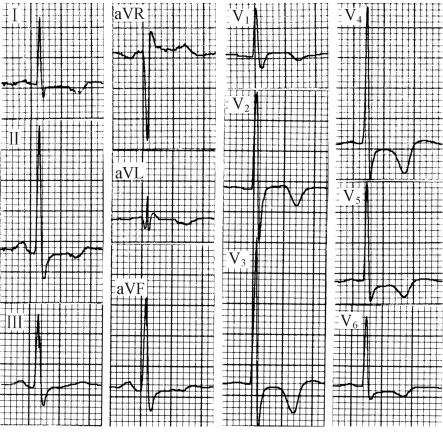
\includegraphics[width=6.67708in,height=3in]{./images/Image00050.jpg}
\end{table}

\subsection{诊断思路}

\subsubsection{病史及体检}

准确而简要的病史询问,全面而有重点的体检,对急性腹痛的诊断十分重要。

\hypertarget{text00026.htmlux5cux23CHP1-10-2-1-1}{}
(一) 年龄、性别、既往史

\paragraph{年龄 、性别}

不同年龄及性别常有不同的多发病,如婴幼儿多见先天性消化道畸形,尤其是胃肠道(肠闭锁或狭窄,肛门闭锁、先天性肥厚性幽门狭窄等)及胆道(先天性胆道闭锁或狭窄);幼儿多见肠寄生虫病、肠套叠、疝嵌顿等;青壮年多见急性阑尾炎、胃肠穿孔、肠梗阻、腹部外伤致脏器破裂内出血等;老年人则胃肠道癌肿及并发症(穿孔、梗阻、出血),胆结石或胆囊炎及血管疾病多见。急性胆道疾病、胰腺炎女多于男,溃疡病穿孔、急性阑尾炎及肠梗阻则男多于女。引起急性腹痛的妇产科疾病,如急性附件或盆腔炎,异位妊娠或破裂,卵巢囊肿蒂扭转,子宫破裂、穿孔等及痛经。

\paragraph{既往史}

应重点询问以往有否引起急性腹痛的病史,有无类似发作史;手术史、月经生产史、外伤史及有害物接触史等。

\hypertarget{text00026.htmlux5cux23CHP1-10-2-1-1-2-1}{}
(1) 有类似发作史者:

应考虑胆石症、胆囊炎、泌尿系结石、慢性阑尾炎或慢性胃炎急性发作,溃疡病活动或出血、穿孔,疝反复嵌顿,胃肠神经症等。

\hypertarget{text00026.htmlux5cux23CHP1-10-2-1-1-2-2}{}
(2) 手术史:

溃疡病胃次全切除术后吻合口溃疡、出血或狭窄,肠粘连或粘连性肠梗阻,膈下或盆腔脓肿等。

女性患者应注意有无痛经史,闭经且发生急性腹痛者应考虑异位妊娠、早期流产,若伴休克,应高度疑及异位妊娠破裂内出血等。

\hypertarget{text00026.htmlux5cux23CHP1-10-2-1-2}{}
(二) 注意腹腔内、外疾病所致急性腹痛的不同特点

\paragraph{腹腔内疾病急性腹痛的特点}

①常伴有消化道症状,如恶心、呕吐、腹泻、腹胀等。②常有与进食有关的诱因,如暴饮暴食、高脂饮食、酗酒、进食过刺激、不洁或变质食物等。③腹部体征较明显且固定(痛、压痛、叩痛、反跳痛等)。④无腹外及全身疾病表现。

\paragraph{外科或妇产科疾病所致急性腹痛的特点}

①腹痛突然发作,剧烈,急剧发展,不及时处理,短期内病情常迅速恶化。②表情痛苦,呻吟,大汗,面色苍白,辗转不安或蜷曲静卧。③可有腹膜刺激征(腹肌紧张呈板状,压痛、反跳痛明显)及肝浊音界缩小或消失。④可有内出血综合征,如头晕、心慌、多汗、面色苍白、脉细速、血压下降等。⑤急诊腹透可见膈下游离气体、高度胀气、鼓肠或胃扩张、梯形液气平面等。⑥发病短期内白细胞明显增高,中性及杆状核增高,中毒血象,进行性贫血等。

\paragraph{内科腹腔脏器疾病所致急性腹痛的特点}

①腹痛可轻可重,短期内病情不恶化。②症状与体征不一致,主观感觉腹痛剧烈,表情痛苦,但检查腹部体征不显著,多腹软,局部轻压痛或压痛,无反跳痛。③发病短期内血象正常或稍高,无中毒血象。④急诊腹透无阳性发现。

\hypertarget{text00026.htmlux5cux23CHP1-10-2-1-3}{}
(三) 依急性腹痛部位诊断

即依据解剖部位来推断可能的病因(表\ref{tab10-2})。最早发生腹痛及压痛最明显的部位常是发生病变的部位(早期及异位阑尾炎例外)。

\hypertarget{text00026.htmlux5cux23CHP1-10-2-1-4}{}
(四) 依病史、体征及伴随症状综合分析

\paragraph{起病方式}

突然发作剧痛,多为胆道蛔虫症、胆道或泌尿道结石嵌顿、疝嵌顿、急性胆囊炎或胰腺炎、消化道急性穿孔、腹腔脏器破裂、急性心肌梗死、心绞痛等。持续性腹痛阵发性加重常示有痉挛或梗阻;初期呈进行性加重多为急性炎症;暴饮暴食、高脂饮食、酗酒、过刺激或不洁食物、激烈运动等诱发急性腹痛应考虑急性胆囊炎、胰腺炎或胃肠炎,溃疡病穿孔,肠或卵巢囊肿蒂扭转,疝嵌顿等。

\paragraph{绞痛及放射痛}

\begin{table}[htbp]
\centering
\caption{急性腹痛部位与疾病关系}
\label{tab10-2}
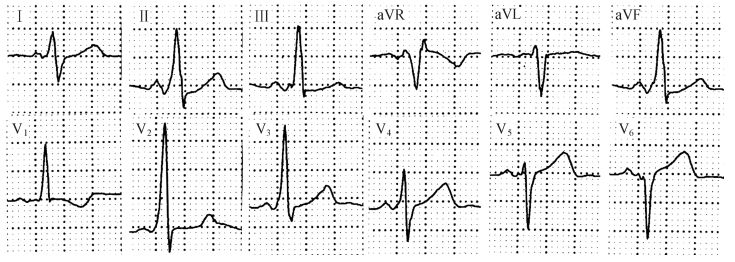
\includegraphics[width=6.71875in,height=3.52083in]{./images/Image00051.jpg}
\end{table}

①胆绞痛:右上腹痛向右肩胛及右背部放射。②胰腺绞痛:上腹或中上腹部向左侧腰背部放射。③小肠绞痛:脐周剧痛。④肾绞痛:肾区痛沿腹直肌外缘向大腿内侧或会阴部放射。⑤子宫或直肠病变绞痛:腰骶部或下腹部剧痛或坠痛。

\paragraph{伴发症状}

\hypertarget{text00026.htmlux5cux23CHP1-10-2-1-4-3-1}{}
(1) 伴发热:

①先发热后腹痛多为不需手术治疗的内科性疾病(常为急性炎症)。②先腹痛后发热的多为外科或妇产科疾病,且常需手术治疗(如急性消化道穿孔、腹膜炎、肠梗阻、异位妊娠破裂、内脏破裂出血等)。③急性腹痛伴寒战、高热,应考虑急性化脓性胆囊炎、胆管炎,腹腔或腹内脏器的化脓性病变(膈下或盆腔脓肿、化脓性腹膜炎),下肺炎症或脓肿等。

\hypertarget{text00026.htmlux5cux23CHP1-10-2-1-4-3-2}{}
(2) 伴呕吐:

急性腹痛伴呕吐者常为急性胃、胆囊、胰腺等炎症,肠梗阻,胆道或泌尿道结石嵌顿,胃型感冒,肠套叠,痛经,神经症等。

\hypertarget{text00026.htmlux5cux23CHP1-10-2-1-4-3-3}{}
(3) 与排便的关系:

①腹痛伴腹泻:急性肠炎、痢疾、急性盆腔炎、急性阑尾炎、高位肠梗阻等。②腹痛伴血便:绞窄性肠梗阻、肠套叠、溃疡性结肠炎、坏死性肠炎、缺血性疾病(栓塞或血栓形成)等。③腹痛伴便秘或停止排便及肛门排气:为习惯或非习惯性便秘、肠梗阻等。

\hypertarget{text00026.htmlux5cux23CHP1-10-2-1-4-3-4}{}
(4) 伴腹胀:

急性胃扩张、麻痹性肠梗阻、便秘、尿潴留等。

\hypertarget{text00026.htmlux5cux23CHP1-10-2-1-4-3-5}{}
(5) 伴黄疸:

①右上腹痛伴黄疸者多为肝、胆系统疾病(炎症、结石、肿瘤等)。②中上腹或左中上腹痛伴黄疸多为胰腺(炎症、结石、肿瘤)或脾脏病变(脾梗死)。③右上腹痛伴寒战、高热、黄疸,应考虑急性胆囊炎,胆结石嵌顿伴炎症,急性化脓性胆囊、胆管炎,急性肝脓肿及少数膈下脓肿。

\hypertarget{text00026.htmlux5cux23CHP1-10-2-1-4-3-6}{}
(6) 与排尿关系:

腹痛伴膀胱刺激征或血尿者多为急性泌尿系感染、结石嵌顿;部分阑尾炎、盆腔脓肿也可引起膀胱刺激征,应注意鉴别。

\hypertarget{text00026.htmlux5cux23CHP1-10-2-1-4-3-7}{}
(7) 与体位的关系:

①辗转不安,腹痛喜按多为胃肠道疾病;拒按多为肝、胆系疾病。②活动疼痛加剧,蜷曲侧卧疼痛减轻多为腹膜炎。③前倾坐位或膝胸位疼痛减轻多为胰腺疾病。

\hypertarget{text00026.htmlux5cux23CHP1-10-2-1-4-3-8}{}
(8) 伴腹水:

①伴血性腹水:腹腔内脏或异位妊娠破裂,恶性肿瘤腹腔内转移,腹膜恶性肿瘤,少数结核性渗出性腹膜炎等。②脓性腹水:化脓性腹膜炎。③胰性腹水:乳糜状,浆液或浆液血性,淀粉酶含量增高且大于血中含量,蛋白量增高,对利尿剂及放腹水疗效差,见于急性出血坏死型胰腺炎或胰腺假囊肿破裂。④胆汁性腹水:化脓性胆囊炎或胆管炎破裂致胆汁性腹膜炎。

\hypertarget{text00026.htmlux5cux23CHP1-10-2-1-4-3-9}{}
(9) 伴休克:

应考虑下列疾病:①急性内出血:腹腔内脏器破裂或异位妊娠破裂。②急性穿孔致弥漫性腹膜炎。③腹腔内脏器或卵巢囊肿蒂扭转。④腹腔内急性血管性病变(肠系膜动脉栓塞或静脉血栓形成)。⑤急性心肌梗死或休克型肺炎。

\hypertarget{text00026.htmlux5cux23CHP1-10-2-1-4-3-10}{}
(10) 伴包块:

应考虑相应部位的急性炎症、肿瘤、肠套叠或扭转。

\hypertarget{text00026.htmlux5cux23CHP1-10-2-1-4-3-11}{}
(11) 与外伤关系:

急性腹痛发生前有外伤史者应考虑腹腔脏器破裂、内出血等。

\subsubsection{辅助检查}

\paragraph{血液检查}

①血红蛋白及红细胞计数:可提示有无内出血致贫血(但早期由于脾脏及骨髓代偿性释放以及血液浓缩,可显示不出贫血或与临床实际贫血程度不符)。②白细胞计数及分类:可提示是否感染、感染程度等。

\paragraph{大便检查}

外观:颜色、性状(成形、糊状、水样、血便、脓血便、黏液便或脓血黏液便等)。镜检:有无红、白细胞,虫卵、真菌、阿米巴滋养体等及潜血试验。

\paragraph{尿液检查}

尿pH、蛋白、糖、酮体、胆红素、红细胞、白细胞、管型、细菌、真菌等,育龄女性应查尿妊娠试验。

\paragraph{生化检查}

依病情需要可作:①血、尿淀粉酶测定;②血钾、钠、氯、钙,血糖,酮体等测定;③肝、肾功能测定等。

\paragraph{心电图检查}

对40岁以上患者,既往无慢性胃病史,突然发作上腹痛应常规作心电图,以识别有无心脏及心包病变。

\paragraph{X线检查}

①胸部X线检查:有助于肺炎、肺脓肿、肺癌、胸膜炎、气胸、肝或膈下脓肿等的诊断。②腹部X线检查:消化道急性穿孔致膈下游离气体,肠梗阻的梯形液气平面,急性胃扩张,高度鼓肠等。另外,胆道或泌尿道阳性结石等。

\paragraph{超声波检查}

B超检查对肝、胆、胰、脾、肾、输尿管、子宫及其附件、盆腔、腹腔等探查均有较强分辨(实质性、囊性、良性、恶性、积液、结石等)及诊断能力,对胃肠道疾病可提供一定的诊断线索。

\paragraph{内镜检查}

急诊内镜检查(胃、十二指肠、胆道、腹腔及结肠镜检查),对急性腹痛的诊断具有极其重要意义。可依临床初步拟诊病变部位,选择相应内镜检查,以助诊断及内镜直视下取活检或治疗。

\paragraph{腹部}

CT检查
主要检查肝、胆、胰、脾、肾、膀胱、腹腔及盆腔等部位,可诊断其形态、大小、密度、占位性病变(实质性、囊性)、结石及腹腔、盆腔有无积液、肿大淋巴结等。

\paragraph{诊断性腹腔穿刺术}

根据穿刺液性质可确定腹膜炎性质,有无内出血(脏器破裂或异位妊娠破裂)等。

\paragraph{阴道后穹隆穿刺术}

主要用于判断异位妊娠破裂出血、盆腔脓肿或盆腔积液。

\subsubsection{急性腹痛的病因诊断线索}

急性腹痛的病因繁多。为尽早明确诊断,应在完成病史采集、体格检查和必要的辅助检查之后,对所得资料进行综合分析,作出正确的病因诊断。下述诊断思路,有助于最终确定病因诊断。

\hypertarget{text00026.htmlux5cux23CHP1-10-2-3-1}{}
(一) 确定是腹腔内病变或腹腔外病变

急性腹痛的诊断 ,首先要确定是腹腔内病变还是腹腔外病变。

\paragraph{腹腔内病变}

常有消化道症状如恶心、呕吐、腹痛、腹泻等,腹痛程度不一,多有较明确诱因。腹部体征依病因而异,一般较明显,腹外与全身性症状轻微或缺乏。

\paragraph{腹腔外病变}

胸部疾病引起的腹痛位于脐上的同侧腹部,可有压痛,但一般无反跳痛及肌紧张,胸部检查可发现有关疾病的心肺体征,胸部X线检查、心电图检查、心肌酶学检查等有助于诊断。全身性疾病所致的腹痛有原发病的表现,腹痛多由于电解质紊乱、代谢失调或毒素刺激所致,位于全腹或部位多变,一般无腹膜刺激征。

\hypertarget{text00026.htmlux5cux23CHP1-10-2-3-2}{}
(二) 确定是外科或非外科急性腹痛

\paragraph{外科急性腹痛}

是指急需外科处理,或病情的发展有需要外科处理可能性的急性腹痛。对急性腹痛患者,应先明确是否为外科急性腹痛。此类腹痛常有以下特点:①剧烈而急起的腹痛多先于发热或呕吐,发热多于腹痛后4~6小时出现,但细菌性肝脓肿、脾脓肿和伤寒肠穿孔等例外。若腹痛超过6小时而患者体温反而降低或低于正常,则应考虑并发休克、大出血或严重感染毒血症的可能。②腹痛部位明确,有固定区,患者多“拒按”腹痛区。③常伴腹膜刺激征。腹痛、固定性压痛点和肌紧张的程度常是越来越严重,提示病变呈进行性发展。④腹式呼吸减弱或消失,肠鸣音亢进或消失,机械性肠梗阻时可闻及高调肠鸣音,而弥散性腹膜炎、麻痹性肠梗阻则肠鸣音减弱或消失。⑤可有肝肺浊音界消失,腹部移动性浊音阳性。⑥腹痛时腹部膨隆或可见胃肠型及蠕动波,并可触及腹部包块或索状物等。⑦腹腔穿刺可有血性或脓性液体等。

\paragraph{内科急性腹痛}

其特点:①一般先有发热或呕吐、腹泻而后出现腹痛。②腹痛可轻可重,腹部体征不明显,无固定而局限性压痛点,无腹膜刺激征。患者常喜按。③腹式呼吸存在,肠鸣音正常或活跃。④可有与腹痛有关的内科疾病的阳性体征。⑤血白细胞正常或升高。

\paragraph{妇产科急性腹痛}

其特点:①由于女性生殖器官集中于下腹部盆腔内,所以妇产科疾病引起的腹痛多局限于中下腹、盆腔,并向会阴和骶尾部放射。②腹痛多与月经、妊娠有关,月经期曾患过上呼吸道感染或有过性生活,多为急性盆腔炎;卵泡破裂多发生在排卵期;宫外孕有停经史,可有早孕反应等。③可伴有腹腔内出血、阴道出血或分泌物增加。④妇科检查常有阳性体征发现。

\paragraph{小儿内科急性腹痛}

其特点:①常以发热、咽痛、咳嗽等症状先于腹痛。②急性腹痛而腹壁柔软,无压痛,腹部无包块、肠型等腹部体征。③腹痛范围广,不规则性,但排便基本正常。④可伴有呕吐等。⑤腹部外疾病引起腹痛者,可发现原发病变部位的阳性体征。

\hypertarget{text00026.htmlux5cux23CHP1-10-2-3-3}{}
(三) 确定急性腹痛的性质

根据常见的病变性质可将急性腹痛归纳为以下七类:

\paragraph{炎症性急性腹痛}

基本特点为:腹痛+发热+压痛或腹肌紧张。

临床特点有:①一般起病较缓慢,多由轻渐重。②持续性腹痛。因脏器或腹膜的炎症、充血、水肿,刺激神经而引起急性腹痛,多呈持续性腹痛进行性加重。因发病的部位、病变程度及其病理变化不同,而呈局限性或全腹性疼痛。疼痛多发生于病变所在的部位。③当炎症病变波及脏器浆膜和壁层腹膜时,则呈典型的局限性或弥漫性腹膜刺激征,即腹肌紧张、压痛和反跳痛,尤其是以病变所在部位最明显。④早期可出现全身感染征象,如寒战、发热、脉快和白细胞增高。⑤腹腔穿刺和灌洗可抽出腹腔炎性渗出物。⑥可有明显的胃肠道刺激症状。此类急腹痛常见的有急性阑尾炎、急性胆囊炎、急性腹膜炎、急性胰腺炎、急性盆腔炎、急性肠系膜淋巴结炎、急性出血性坏死性肠炎等。

\paragraph{穿孔性急性腹痛}

基本特点是:突发持续腹痛+腹膜刺激征,可伴有肠鸣音消失或气腹。

由外伤、炎症或癌肿侵蚀等导致空腔脏器破裂所致。其临床特点有:①突然剧烈的刀割样腹痛,后呈持续性,范围迅速扩大。②腹壁板样强直,有明显腹膜刺激征,常伴有休克。③常见膈下游离气体和腹部移动性浊音。④肠鸣音消失。例如消化性溃疡穿孔、胃癌穿孔、胆囊穿孔、伤寒肠穿孔、外伤性肠穿孔等。

\paragraph{梗阻性急性腹痛}

基本特点是:阵发性腹痛+呕吐+腹胀+排泄功能障碍。

肠道、胆道、输尿管等空腔管道内结石、肿瘤和位置改变(如扭转、套叠)等因素阻塞,腔内压增高促使管腔道平滑肌强烈收缩以排除障碍,发展到血运障碍(如绞窄性疝等),或始发于血运障碍(如肠系膜血管阻塞等),继发缺血、坏死等变化,即发生梗阻性急腹痛。其临床特点有:①阵发性腹部剧痛是其特征,多突然发生,呈阵发性剧烈绞痛,往往使患者难以忍受。当梗阻器官合并炎症或血运障碍时,常呈持续性腹痛,阵发性加重。②恶心、呕吐,早期是反射性,后期是逆流性呕吐。因梗阻发生的部位不同,呕吐的内容和量亦不同。胃肠道高位梗阻则早发频吐,多为胃及十二指肠内容物;低位梗阻则晚发溢吐,严重者可呕吐粪性内容物。③腹胀和梗阻的器官管型明显,此因梗阻的器官、部位、程度和病变性质不同而表现亦异:如幽门梗阻表现上腹胀、振水音,可见胃蠕动波;肠梗阻可见腹胀、肠型、蠕动波;胆道梗阻出现胆囊肿大或胆管扩张;泌尿系梗阻出现膀胱区域或肾区的囊性肿块等。④正常排泄功能障碍。胃肠道梗阻出现呕吐、肛门停止排便排气;胆道梗阻出现黄疸;泌尿系梗阻则呈现尿少或尿潴留、肾积水等。⑤除泌尿系疾病外,多伴有水、电解质与酸碱平衡失调、休克,或晚期毒血症。此类急性腹痛常见的有肾、输尿管结石、肝内胆管结石、肝外胆管结石、胆绞痛、胆道蛔虫病、肠梗阻、肠套叠、嵌顿性腹股沟疝、嵌顿性股疝、卵巢囊肿蒂扭转等。

\paragraph{出血性急性腹痛}

其基本特点是:腹痛+失血性休克与急性贫血+隐性(内)出血或显性(外)出血(呕血、便血或尿血)。

腹内实质脏器或血管因外伤或病变发生破裂引起腹腔内出血,由于大量积血刺激导致急性腹膜炎,但腹膜刺激症状较轻,无感染症状,而有急性失血症状。临床特点有:①可有肝癌、消化性溃疡、腹主动脉瘤、输卵管妊娠以及肝、脾外伤等病史。②起病较急骤,腹痛为持续性,但不及炎症性或穿孔性腹痛剧烈。③外观可见的出血,如呕血、便血、尿血等,或胃肠吸引、导尿、肛管直肠或阴道内诊等证实有内出血者。④虽无外观出血,但证实有内出血:进行性贫血;腹部有移动性浊音,腹腔穿刺抽出不凝固的血液。⑤有失血性休克表现。⑥B超可探及腹腔内液性暗区及受损伤的脏器。此类急性腹痛常见的有消化性溃疡出血、外伤性肝脾破裂出血、胆道出血、肝癌破裂出血、腹主动脉瘤破裂大出血、异位妊娠破裂出血等。

\paragraph{损伤性急性腹痛}

其基本特点是:外伤+腹痛+腹膜炎或内出血综合征。

腹部损伤,因暴力及着力点不同,可有腹壁伤,如挫伤、肌肉撕裂伤、腹壁血肿形成;空腔脏器伤,如胃、小肠、大肠、胆囊、膀胱破裂等;以及实质性脏器伤,如肝、脾、胰、肾损伤等。临床特点有:①有外伤史,尤其是腹部、腰部和下胸部外伤。②腹痛,原发性休克恢复后,常呈现急性持续性剧烈腹痛,伴恶心、呕吐。③内出血征象:烦躁不安、面色苍白、出冷汗、口渴、脉搏细速、血压进行性下降,重者出现休克;腹部有移动性浊音,腹穿可抽出新鲜或暗红色不凝固的血液。④腹膜炎综合征:恶心、呕吐、腹痛、腹肌紧张,压痛、反跳痛明显;腹穿抽出物可为消化道分泌物或腹性分泌物。⑤X线检查:腹内脏器移位、阴影扩大或消失、膈下游离气体、腹内积液或积气。

\paragraph{绞窄与扭转性急性腹痛}

这是由于肠道(如小肠、乙状结肠)、较活动的脏器(如游离的脾、肾等)、有蒂肿瘤(如卵巢囊肿)、腹内、外疝等发生扭转及绞窄,引起缺血、组织坏死和血性渗液,亦称缺血性急腹痛。临床特点有:①腹痛为持续性,因受阵发牵拉,可有阵发性类似绞痛的加剧。②常可触及压痛性包块。③早期无腹膜刺激征,随着坏死的发生而出现。④可有频繁干呕,消化道排空症状如频繁便意,排气,也可排出肠道黏液或黏液血便等。

\paragraph{功能性紊乱及全身性疾病所致的急性腹痛}

临床特点有:①常有精神因素或全身性疾病史。②腹痛常无明确定位,呈间歇性、一过性或不规则性。③腹痛虽严重,但体征轻,腹软,无固定压痛和反跳痛。如食管弥漫性痉挛、胆道运行功能障碍、结肠肝(脾)曲综合征、游走肾、肠道易激综合征、胃肠神经症等;全身性疾病如肠系膜动脉硬化或缺血性肠病,结缔组织病累及胃肠道、血卟啉病、腹型癫痫、过敏性紫癜等。

\subsection{处理原则}

\subsubsection{急性腹痛的处理原则}

\paragraph{快速评估}

迅速检查呼吸、脉搏、血压、神志和体温,把急性腹痛分为三类:①危重:先救命后治病。如腹主动脉瘤破裂、异位妊娠破裂并重症休克等。要在快速纠正休克的同时急诊手术或介入治疗控制出血。②重:诊断与治疗相结合。如绞窄性肠梗阻、消化道穿孔、卵巢囊肿蒂扭转等。要在尽快完成各项有关检查的同时,纠正一般情况,准备急诊手术和相关治疗。③普通(可有潜在危险性):寻找危及生命潜在原因。如胃肠炎、消化道溃疡、慢性炎症、腹壁神经性或肌肉疼痛,也可能是恶性肿瘤,结石等。按常规诊疗程序进行采集病史、体格检查、辅助检查、诊断、鉴别诊断。

\paragraph{急性腹痛病因未明者}

对病因不明的急性腹痛患者,应密切观察,辅以必要的辅助检查,以尽早作出诊断,同时给予积极的对症支持疗法。

\hypertarget{text00026.htmlux5cux23CHP1-10-3-1-2-1}{}
(1) 严密观察护理、有目的有计划地追踪诊断:

对诊断不明的急性腹痛患者,切忌主观片面、放任自流,应认真做到“三严”,即严肃追踪观察、严密护理和严格做好临床交接班工作,尤其是对下述情况更应该提高警惕:①特殊的阑尾炎,如老、幼、孕妇或异位阑尾炎;②易被忽略的妇女嵌顿性斜疝或股疝;③绞痛后尚可排便的肠梗阻,如肠套叠、不全肠梗阻或高位肠梗阻;④外伤史很轻或无外伤史的自发性肝、脾破裂,肝或脾包膜下血肿继发大出血等;⑤无胃病史或无气腹的消化性溃疡穿孔、出血,早期症状轻的小穿孔或穿孔后暂时好转期的患者;⑥多发性损伤患者,尤其是易被忽略的并发闭合性腹部损伤;⑦某些病史不详的患者如休克、昏迷和婴幼儿等。对这类患者,必须严密追踪观察病情变化,多次重复检查与估计病情,以便尽早明确诊断,指导治疗。动态观察的重点内容有:①生命体征:体温、脉搏、呼吸、血压和神志的变化;②腹部情况:腹痛的部位、性质、范围、程度以及腹膜刺激征的变化等;③心、肺、肝、肾、脑等重要脏器的功能变化;④胃肠道功能状态:饮食、呕吐、腹泻、排便情况、腹胀、肠蠕动、肠鸣音等;⑤腹腔的异常,如腹腔积气、积液、肝浊音界变化和移动性浊音;⑥新的症状与体征的出现等。严密观察期间,应禁食、禁忌止痛、禁用泻药、禁止灌肠等“四禁”。其目的是为了避免加重病情,防止掩盖症状而妨碍临床观察病情变化,防治并发症。若病情必须使用镇痛剂,可先试用阿托品、654-2等抗胆碱药物,严禁使用吗啡、哌替啶(度冷丁)等麻醉剂。但近年来有学者研究认为,早期正确有效地使用止痛剂不仅可以较大程度地减轻患者的疼痛,不影响患者的诊断和治疗,还有助于患者配合各项检查,提高诊断的准确性。

\hypertarget{text00026.htmlux5cux23CHP1-10-3-1-2-2}{}
(2) 对症支持疗法:

①纠正水、电解质紊乱;②抗感染:对有发热、白细胞总数及中性粒细胞增高的炎症性疾病患者,及时使用有效抗生素对疾病转归有积极作用;③防治腹胀:通常采用的措施是禁饮食,持续有效的胃肠减压等;④防止休克等。

\hypertarget{text00026.htmlux5cux23CHP1-10-3-1-2-3}{}
(3) 剖腹探查指征:

①疑有腹腔内出血不止;②疑有肠坏死或肠穿孔而有严重腹膜炎;③经密切观察和积极治疗后,腹痛不缓解,腹部体征不减轻,全身情况无好转反而加重。

\paragraph{急性腹痛的病因明确者}

立即作病因治疗(包括手术治疗等)。如对肠梗阻、内脏穿孔或出血、急性阑尾炎等有手术指征者,应及时手术治疗。对腹痛能忍受者一般不用镇痛剂,但对病因已明确而不需手术治疗、疼痛较剧的患者,应适当使用镇痛剂,有利于病情恢复。可根据腹痛的性质与程度选用药物,如肝胆胰疾病或输尿管结石所致的疼痛多采用吗啡、哌替啶与阿托品合用;消化性溃疡疼痛宜用抗酸、解痉剂及H\textsubscript{2}
受体阻滞剂等抗溃疡药物治疗;功能性腹痛多用解痉剂和精神安定剂等。急性腹痛的处理程序见图\ref{fig10-1}。

\subsubsection{常见急性腹痛危重情况的诊治}

\paragraph{急性腹痛伴失血性休克}

\hypertarget{text00026.htmlux5cux23CHP1-10-3-2-1-1}{}
(1) 临床表现特点:

①交感兴奋症状:精神紧张、脉快、苍白、额头冷汗、手指冰冷;②末梢循环障碍:甲床青紫、当压迫患者甲床和耳垂后毛细血管再充盈缓慢;轻压患者的前臂时,患者的手背静脉不易充盈、尿少等;③脉搏细速、血压下降;④中心静脉压和心脏排出量降低。

\hypertarget{text00026.htmlux5cux23CHP1-10-3-2-1-2}{}
(2) 治疗原则:

①积极进行抗休克治疗。②需要进行紧急剖腹手术以控制出血。

\begin{figure}[!htbp]
 \centering
 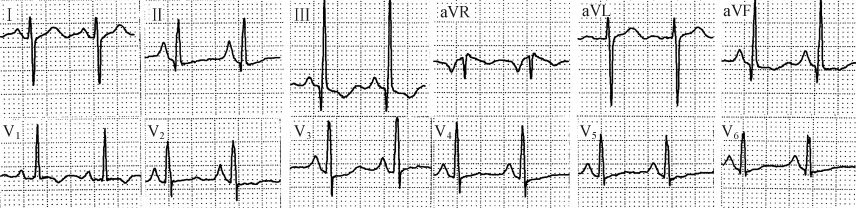
\includegraphics[width=4.71875in,height=4.10417in]{./images/Image00052.jpg}
 \captionsetup{justification=centering}
 \caption{急性腹痛的处理程序}
 \label{fig10-1}
  \end{figure} 

\paragraph{急性腹痛伴感染性休克}

\hypertarget{text00026.htmlux5cux23CHP1-10-3-2-2-1}{}
(1) 临床表现特点:

①重度中毒表现如寒战,体温迅速升高,精神萎靡,意识障碍等;②休克征象表现为面色苍白,血压下降、尿量减少,脉搏细速,末梢循环不良等;③白细胞明显升高或低于正常甚至核左移。

\hypertarget{text00026.htmlux5cux23CHP1-10-3-2-2-2}{}
(2) 治疗原则:

①扩充血容量,静脉输液;②给予抗生素治疗;③物理方法降温;④寻找感染灶的可能部位并及时处理。

\paragraph{继发性急性腹膜炎}

继发性急性腹膜炎是指由各种腹腔内病变或外伤所继发的腹膜急性炎症。

\hypertarget{text00026.htmlux5cux23CHP1-10-3-2-3-1}{}
(1) 临床表现特点:

①最突出的症状是腹痛,多为突然发病;常表现为持续性、烧灼样疼痛,随身体的活动而加剧。在炎症最明显处疼痛最重。疼痛范围缩小、程度减轻时,提示炎症局限;反之,则表明炎症扩散。②其他常见症状包括恶心、呕吐、食欲不振、口渴和自觉发热等,发病后患者多表现为尿少和便秘。③急性腹膜炎的特异性体征------腹膜刺激征:肌紧张、压痛和反跳痛。④中毒症状:疾病的早期,患者的体温往往增高并不明显,随着病程的进展,患者体温可以逐渐增高到38℃以上。甚至出现中毒性休克。⑤在空腔脏器穿孔的病例,可出现气腹征------肺肝界叩不清或消失,腹透时隔下有游离气体。⑥腹部穿刺:对诊断非常有帮助。通过对吸出的腹腔液性状进行观察,常可以判断出腹膜炎的病因。

\hypertarget{text00026.htmlux5cux23CHP1-10-3-2-3-2}{}
(2) 治疗原则:

①动态监测患者的病情变化、胃肠减压并留置尿管导尿;②补充血容量、应用抗生素;③积极处理原发病,及时手术处理。

\protect\hypertarget{text00027.html}{}{}

\hypertarget{text00027.htmlux5cux23CHP1-10-4}{}
参 考 文 献

1. 高德明 ,吴金生.现代急腹症学.北京:人民军医出版社,2002

2. Lo Vecchio F,Oster N,Sturmann K,et al. The use of analgesics in
patient with acute abdominal pain. J Emerg Med,1997,15 (6):775

3.
周玲君,刘红香,赵继军.急腹症的早期止痛.中华急诊医学杂志,2006,15(1):91

4. Lo Vecchio F,Oster N,Sturmann K,et al. The use of analgesics in
patient with acute abdominal pain. J Emerg Med,1997,15 (6):775

5. 刘保池 .急腹症的正确诊断与处理.国际外科学杂志,2008,35(6):369

\protect\hypertarget{text00028.html}{}{}

\chapter{恶心与呕吐}

恶心(nausea)、呕吐(vomiting)是临床上常见的症状之一。恶心是一种特殊的主观感觉,表现为胃部不适和胀满感,常为呕吐的前奏,多伴有迷走神经兴奋的症状,如皮肤苍白、流涎、出汗、血压降低及心动过缓等;呕吐是一种胃的反射性强力收缩,通过胃、食管、口腔、膈肌和腹肌等部位的协同作用,能迫使胃内容物由胃、食管经口腔急速排出体外。从某种意义上来说呕吐是机体的一种保护性作用,它可把对机体有害的物质排出体外,但实际上很多呕吐并非摄入有害物质引起,而且频繁和剧烈的呕吐,可引起失水、电解质紊乱和营养障碍。

\subsection{病因与发病机制}

\subsubsection{病因}

引起恶心、呕吐的病因很广泛,包括多方面因素,几乎涉及各个系统。

\paragraph{感染}

病毒性急性胃肠炎、细菌性急性胃肠炎、急性病毒性肝炎、阑尾炎、胆囊炎、腹膜炎、急性输卵管炎、盆腔炎等。

\paragraph{腹腔其他脏器疾病}

①脏器疼痛:胰腺炎、胆石症、肾结石、肠缺血、卵巢囊肿蒂扭转。②胃肠道梗阻:幽门梗阻(溃疡病、胃癌、腔外肿物压迫)、十二指肠梗阻(十二指肠癌、胰腺癌)、肠粘连、肠套叠、绞窄疝、克罗恩病、肠结核、肠道肿瘤、肠蛔虫、肠扭转、肠系膜上动脉压迫综合征、输出袢综合征、胃肠动力障碍(糖尿病胃轻瘫、非糖尿病胃轻瘫)、假性肠梗阻(结缔组织病、糖尿病性肠神经病、肿瘤性肠神经病、淀粉样变等)。

\paragraph{内分泌代谢性疾病}

低钠血症、代谢性酸中毒、营养不良、维生素缺乏症、糖尿病酸中毒、甲状腺功能亢进、甲状腺功能低下、甲状旁腺功能亢进症、垂体功能低下、肾上腺功能低下,各种内分泌危象、尿毒症等。

\paragraph{神经系统疾病}

中枢神经系统感染(脑炎、脑膜炎)、脑肿瘤、脑供血不足、脑出血、颅脑外伤、脑寄生虫病等。

\paragraph{药物等理化因素}

麻醉剂、洋地黄类、化疗药物、抗生素、多巴胺受体激动药、非甾体抗炎药、茶碱、酒精、放射线等。

\paragraph{精神性呕吐}

神经性多食、神经性厌食。

\paragraph{前庭疾病}

晕动症、梅尼埃病、内耳迷路炎。

\paragraph{妊娠呕吐}

妊娠剧吐、妊娠期急性脂肪肝。

\paragraph{其他}

心肺疾患(心肌梗死、肺梗死、高血压、急性肺部感染、肺心病)、泌尿系疾患(急性肾炎、急性肾盂肾炎、尿毒症)、周期性呕吐、术后恶心呕吐、青光眼。

\subsubsection{发病机制}

这是一系列复杂的反射动作,可分为三个阶段,即恶心、干呕与呕吐。恶心发生时,唾液分泌增加,胃蠕动减弱或者消失、排空延缓,十二指肠及近端空肠紧张性增加,出现逆蠕动,导致十二指肠内容物反流至胃内。干呕时胃上部放松而胃窦部短暂收缩;呕吐时胃窦部持续收缩,下食管括约肌松弛,腹肌收缩,膈肌下降,腹压增加,迫使胃内容物急速而猛烈地从胃反流,经食管、口腔而排出体外。呕吐与反食不同,后者系无恶心与呕吐的协调动作而使胃内容物一口一口地反流到口腔。

目前认为的主要的反射通路包括:①信息传入:由自主神经传导(其中迷走神经纤维较交感神经纤维起的作用大)。②呕吐反射中枢:目前认为中枢神经系统的两个区域与呕吐反射密切相关。一是延髓呕吐中枢,另一是化学感受器触发区(chemical
trigger zone,CTZ)。③传出神经:包括迷走神经、交感神经、体神经和脑神经。

通常把内脏末梢传来的冲动引起的呕吐称为反射性呕吐,把CTZ受刺激后引起的呕吐称为中枢性呕吐。延髓呕吐中枢位于延髓外侧网状结构背外侧,迷走神经核附近,主要接受来自消化道和内脏神经、大脑皮质、前庭器官、视神经、痛觉感受器和化学感受区的传入冲动。化学感受器触发区(CTZ)位于第四脑室底部的后极区,为双侧性区域,有密集多巴胺受体。多巴胺受体在CTZ对呕吐介导过程中起重要作用,因为应用阿扑吗啡、左旋多巴、溴隐亭等多巴胺受体激动药可引起呕吐,而其拮抗药、甲氧氯普胺(胃复安)、吗丁啉等药物有止呕作用。化学感受器触发区的5-羟色胺、去甲肾上腺素、神经肽物质和γ-氨基丁酸等神经递质也可能参与呕吐反射过程。CTZ主要接受来自血液循环中的化学、药物等方面的呕吐刺激信号,并发出引起呕吐反应的神经冲动。但CTZ本身不能直接引起呕吐,必须在延髓呕吐中枢完整及其介导下才能引起呕吐,但两者的关系尚不十分明确。CTZ位于血-脑脊液屏障之外,许多药物或代谢紊乱均可作用于CTZ。某些药物如麻醉剂、化学药物、麦角衍生物类药、吐根糖浆等及体内某些多肽物质如甲状腺激素释放激素、P物质、血管紧张素、胃泌素、加压素、血管肠肽等均可作用于CTZ引起恶心呕吐。此外,某些疾病如尿毒症、低氧血症、酮症酸中毒、放射病、晕动症等引起的恶心呕吐也与CTZ有关。

传出神经的呕吐信号传至效应器官,引起恶心呕吐过程,呕吐开始时,幽门关闭,胃内容物不能排到十二指肠,同时,贲门口松弛,贲门部上升,腹肌,膈肌和肋间肌收缩,胃内压及腹内压增高,下食管括约肌松弛,导致胃内容物排出体外。

\subsection{诊断思路}

\subsubsection{病史}

\paragraph{药物或放射线接触史}

易引起呕吐的常用药物有某些抗生素、洋地黄、茶碱、化疗药物、麻醉剂、酒精等。镭照射线治疗和钴照射线治疗,常引起恶心呕吐。

\paragraph{其他}

呕吐可为许多系统性疾病的表现之一,包括糖尿病、甲状腺功能亢进症或甲状腺功能减退症、肾上腺功能减退等内分泌疾病、硬皮病等结缔组织病、脑供血不足、脑出血、脑瘤、脑膜炎、脑外伤等中枢神经系统疾病、尿毒症等肾脏疾病。

\subsubsection{临床表现特点}

\paragraph{呕吐的伴随症状}

呕吐伴发热者,须注意急性感染性疾病;呕吐伴有不洁饮食或同食者集体发病者,应考虑食物或药物中毒;呕吐伴胸痛,常见于急性心肌梗死或急性肺梗死等;呕吐伴有腹痛者,常见于腹腔脏器炎症、梗阻和破裂;腹痛于呕吐后暂时缓解者,提示消化性溃疡、急性胃炎及肠道梗阻性疾病;呕吐伴头痛,除考虑颅内高压的疾患外,还应考虑偏头痛、鼻炎、青光眼及屈光不正等疾病;呕吐伴眩晕,应考虑前庭、迷路疾病、基底椎动脉供血不足、小脑后下动脉供血不足及某些药物(氨基糖苷类抗生素)引起的脑神经损伤。

\paragraph{呕吐的方式和特征}

喷射性呕吐多见于颅内炎症、水肿出血、占位性病变、脑膜炎症粘连等所致颅内压增高,通常不伴有恶心。此外,青光眼和第Ⅷ对脑神经病变也可出现喷射性呕吐。呕吐不费力,餐后即发生,呕吐物量少,见于精神性呕吐。应注意呕吐物的量、颜色和气味等。呕吐物量大,且含有腐烂食物提示幽门梗阻伴胃潴留、胃轻瘫及小肠上端梗阻等;呕吐物为咖啡样或血性见于上消化道出血,含有未完全消化的食物则提示食管性呕吐(贲门失弛缓症、食管憩室、食管癌等)和见于神经性呕吐、胆囊炎、胆石症及胃大部切除术后等,有时见于妊娠剧烈呕吐、晕动症;呕吐物有酸臭味者,或胃内容物有粪臭味提示小肠低位梗阻、麻痹性肠梗阻、结肠梗阻而回盲瓣关闭不全或胃结肠瘘等。

\paragraph{呕吐和进食的时相关系}

进食过程或进食后早期发生呕吐,常见于幽门管溃疡或精神性呕吐;进食后期或餐后呕吐,见于幽门梗阻、肠梗阻、胃轻瘫或肠系膜上动脉压迫导致十二指肠雍积;晨起呕吐多见于妊娠呕吐,有时亦见于尿毒症、慢性酒精性中毒和颅内高压等。

\subsubsection{体格检查}

\paragraph{一般情况}

应注意神志、营养状态、有无脱水、循环衰竭、贫血及发热等。

\paragraph{腹部体征}

应注意胃型、胃蠕动波、振水声等幽门梗阻表现:肠鸣音亢进、肠型等急性肠梗阻表现:腹肌紧张、压痛、反跳痛等急腹症表现。此外,还应注意有无腹部肿块、疝等。

\paragraph{其他}

①眼部检查注意眼球震颤、眼压测定、眼底有无视乳头水肿等。②有无病理反射及腹膜刺激征等。

\subsubsection{实验室检查}

主要包括与炎症、内分泌代谢及水盐电解质代谢紊乱等有关的实验室检查。

\subsubsection{其他辅助检查}

可做B超、胃镜、ERCP、超声内镜、CT、磁共振等特殊检查。

\subsection{治疗}

由于引起恶心、呕吐的疾病很多,恶心、呕吐仅是疾病的症状之一。因此,在未明确病因之前不应盲目应用作用于呕吐中枢的强镇吐药物,否则会贻误病情。只有在明确了导致呕吐的病因之后,在积极治疗病因的基础上,才能行必要的对症治疗。

\paragraph{胃肠道疾病}

包括食管、胃、十二指肠直至空肠、回肠、结肠及直肠在内的任何部位的病变都有可能引起恶心、呕吐的症状,其中以食管狭窄、食管癌、贲门失弛缓、贲门癌、胃窦部嗜酸性肉芽肿、胃窦部巨大溃疡或癌肿、十二指肠溃疡或郁积症、多种原因导致的小肠与大肠梗阻或急性胃、小肠或大肠的炎症性病变为最常见的病因。因消化道良性或恶性病变造成的狭窄或梗阻所致的呕吐,药物治疗是无效的,只有经扩张、置入支架或手术治疗,解除狭窄或梗阻之后,呕吐症状才会消失。对于贲门失弛缓症患者,在未进行扩张或手术治疗之前,可选用钙离子通道拮抗药或硝酸甘油餐前半小时口服或餐前15~30分钟舌下含化治疗,早期可改善呕吐及梗阻症状:或者试用肉毒杆菌毒素行狭窄局部注射治疗。胃肠道急性炎症性病变引起的呕吐,应积极选用抗生素并纠正电解质紊乱及补充维生素;胃肠动力障碍引起的恶心与呕吐则可应用莫沙比利(mosapride,5mg口服,每日3次)、西沙比利(cisapride,5~10mg口服,每日2~4次)、多潘立酮(吗丁啉,10~20mg口服,每日3次;或10mg肌肉注射)、甲氧氯普胺(灭吐灵,胃复安,5~10mg口服;或10~20mg肌肉注射。每日剂量应≤0.5mg/kg,否则易引起锥体外系反应)等促胃肠动力剂;如果呕吐是由胃肠道痉挛所致,则可应用东莨菪碱(0.3mg口服或注射)等抗胆碱能药物。

\paragraph{肝脏 、胆道及胰腺疾病}

是导致恶心、呕吐的常见病因之一。恶心、呕吐可是急性病毒性肝炎的早期症状,常与食欲减退、厌油腻食物及上腹部饱胀同时出现,随着护肝治疗及适当的休息之后,恶心与呕吐可逐渐消失。呕吐也是胆道梗阻或绞痛常伴随的症状,只有当胆道梗阻或炎症消除之后,呕吐才会停止;急性胰腺炎时常伴随有恶心与呕吐症状,只有随着采用胃肠减压、减少胰液分泌等措施之后,呕吐才会逐步缓解或终止。

\paragraph{中枢神经系统病变}

包括各种原因所致的脑炎、脑膜炎、脑肿瘤、脑寄生虫病、脑血管病及颅脑外伤等病变,均可引起颅内压力增高而导致恶心、呕吐。治疗的重要措施之一就是应用降低颅内压、减轻脑细胞水肿的药物治疗。脱水治疗后,不仅可改善呕吐的症状,更重要的是起到了保护或恢复脑细胞功能的作用。

\paragraph{药物所致的呕吐}

多种药物有引起恶心与呕吐的不良反应,一般而言,只要立即停止应用引起呕吐的药物,呕吐症状就会减轻直至消失,因此并不需要应用镇吐类药物。目前临床上对某些恶性肿瘤或血液系统的恶性疾病(如白血病、恶性淋巴瘤、多发性骨髓瘤、恶性组织细胞病等)采用联合化疗或放疗,或对某些恶性肿瘤采用抗癌药物行介入治疗。但无论在治疗过程中或治疗之后,均可引起较为严重的胃肠道不良反应,最突出的表现就是恶心与呕吐。为了预防或减轻此不良反应,常可应用镇吐药物进行治疗,常用的药物有昂丹司琼(ondansetron,奥丹西龙,商品名:枢复宁。常用8mg口服或静脉注射)、格拉司琼(granisetron,商品名:康泉。成人剂量每次40μg/kg,或标准剂量3mg,静脉滴注)等。必须指出,应用这些作用强的镇吐药物之后,也会产生中枢神经系统、心血管系统或胃肠道的不良反应,故应严格控制药物剂量及间隔时间。

\paragraph{神经 、精神因素所致的呕吐}

对此类原因所致的呕吐,心理治疗是关键。首先应消除患者的精神心理障碍,其次可配合药物治疗,常用的药物是镇静药与胃肠促动力剂、重者可采用多塞平或氟西汀等抗抑郁药物治疗。禁忌应用昂丹司琼(奥丹西龙)等强烈作用的镇吐药。

\protect\hypertarget{text00029.html}{}{}

\hypertarget{text00029.htmlux5cux23CHP1-11-4}{}
参 考 文 献

1. 陈文彬,潘祥林.诊断学.第7版.北京:人民卫生出版社,2008

2. 陈新谦,金有豫,汤光.新编药物学.第17版.北京:人民卫生出版社,2011

\protect\hypertarget{text00030.html}{}{}

\chapter{急 性 腹 泻}

正常人一般每日排成形大便1次,粪便平均重量为150~200g,一般不超过200g,其中水分占60\%~70\%,约150ml左右。少数人每天排便2~3次或2~3天才排1次,但若粪质成形,性状与常人无异,亦属正常。

腹泻(diarrhea)是指排便习惯和粪便性状发生变化,排便次数增多(每天3次以上),粪质稀薄,水分增加(水分超过85\%),粪便量增加(超过200g/d)。便质不成形、稀溏或呈液状,有时含有脓血或带有未消化食物及脂肪。确定是否有腹泻应根据个体的大便习惯而异。

腹泻可根据病程分为急性腹泻和慢性腹泻两种,也可依病因分为感染性腹泻和非感染性腹泻两大类。急性腹泻是指起病急骤、病程较短,病程在2~3周之内,极少超过6~8周。慢性腹泻指病程至少在4周以上,常超过6~8周,或间歇期在2~4周内的复发性腹泻。腹泻常伴有排便紧迫感、肛门不适或大便失禁。腹泻可导致水电解质丢失,严重时可引起大量失水,导致低血容量性休克和急性器官功能衰竭,甚至因电解质严重紊乱引起严重心律失常而死亡。

\subsection{病因与发病机制}

在禁食期间,正常人肠腔内液体含量很少。但正常三餐摄取后,每天约有9L液体进入肠道,其中2L来自进食的食物和饮料,其余来自消化道分泌液,包括唾液1.5L、胃液2.5L、胰液1.5L、胆汁0.5L和小肠液1.0L。进入胃肠道的食糜在通过小肠时,食糜的渗透度变得与血浆相同,其中90\%的水分被其吸收。食糜在到达回肠末端时,已呈等渗状态,每天仅有1~2L的液体进入结肠,而结肠也具有强大的吸收水分的功能,使大便最终含水量只有100~200ml。若胃肠道的分泌、消化、吸收和运动等功能障碍,使消化道分泌的液量增加,食物不能完全分解,吸收量减少和肠胃蠕动加速等,最终可导致粪便性状稀薄、次数增加而形成腹泻。腹泻的发病机制相当复杂,从病理生理角度分为四类,部分腹泻的发病可有几个因素并存,具体如下:

\paragraph{分泌性腹泻}

肠道液体主要由黏膜隐窝细胞分泌,大部分经肠绒毛腔面上皮细胞吸收。当各种刺激因子刺激肠黏膜细胞分泌的量超过其吸收能力时,所引起的腹泻称分泌性腹泻(secretory
diarrhea)。刺激肠黏膜分泌的因子可分为四类:①细菌的肠毒素,如霍乱弧菌、大肠埃希菌、沙门菌等毒素;②神经体液因子,如血管活性肠肽(VIP)、血清素、降钙素等;③免疫炎性介质,如前列腺素、白三烯、血小板活化因子、肿瘤坏死因子、白介素等;④去污剂,如胆盐和长链脂肪酸,通过刺激阴离子分泌和增加黏膜上皮通透性而引起分泌性腹泻;⑤各种通便药,如蓖麻油、酚酞、芦荟、番泻叶等均可引起分泌性腹泻。

肠道分泌电解质和水分的机制相当复杂。近年发现,肠黏膜隐窝细胞中的第二信使如环磷酸腺苷(cAMP)、环磷酸鸟苷(cGMP)、钙离子等的增加是诱导黏膜隐窝细胞分泌的重要环节。霍乱弧菌和致病性大肠埃希菌的毒素首先与上皮细胞刷状缘上的受体结合,激活腺苷环化酶-cAMP系统,致cAMP浓度增高,引起大量肠液分泌;艰难梭菌(C.difficile)是通过钙离子增加而引起分泌性腹泻;血管活性肽瘤(VIP瘤)引起的腹泻是一种非感染性的分泌性腹泻,肿瘤释出的VIP能激活肠黏膜的腺苷酸环化酶,刺激小肠大量分泌液体,故而出现霍乱样的严重水泻,称为胰性霍乱,常伴有严重的低钾血症和代谢性酸中毒;胃泌素瘤能分泌大量的胃泌素,刺激壁细胞分泌大量胃液,过多胃液进入小肠后,不仅可损害空肠黏膜,而且促进肠道蠕动,使胰脂肪酶灭活,脂肪消化障碍而更加重腹泻。分泌性腹泻还可见于直肠分泌性绒毛状腺瘤、肠淋巴瘤、炎症性肠病、肠肉芽肿性疾病、结缔组织病、恶性类癌综合征、甲状腺髓样癌等。

分泌性腹泻的特点是:①禁食不减轻腹泻;②肠液与血浆的渗透压相同;③大便呈水样,量多,无脓血;④一般不伴有腹痛;⑤肠黏膜组织学基本正常。

\paragraph{渗透性腹泻}

由于肠腔内含有大量不能被吸收的溶质,导致肠腔内渗透压升高,大量液体被动进入肠腔而引起腹泻,称为渗透性腹泻(osmotic
diarrhea)或吸收不良性腹泻(malabsorption diarrhea)。见于:

\hypertarget{text00030.htmlux5cux23CHP1-12-1-2-1}{}
(1) 高渗性药物:

口服镁盐、乳果糖、甘露醇或山梨醇等高渗性药物。

\hypertarget{text00030.htmlux5cux23CHP1-12-1-2-2}{}
(2) 高渗性食物:

主要是某些碳水化合物,由于水解酶缺乏或其他原因而导致食物吸收不良,形成高渗透压性的肠内容物而引起腹泻。临床上最常见的是原发性乳糖酶缺乏,患者口服牛奶或奶制品后即可引起腹泻。

\hypertarget{text00030.htmlux5cux23CHP1-12-1-2-3}{}
(3) 消化不良:

胃大部分切除术后、萎缩性胃炎和胃癌患者的胃液分泌减少,慢性胰腺炎、胰腺切除术后使胰液分泌减少,严重肝病或胆管梗阻可导致胆汁分泌或排泄减少,使食物不能充分被消化,营养物质不能被吸收,致使高渗性肠内容物增多而造成腹泻。

\hypertarget{text00030.htmlux5cux23CHP1-12-1-2-4}{}
(4) 吸收不良:

①黏膜透过性异常:由于小肠黏膜细胞的特殊病变如绒毛或微绒毛的变形、萎缩等变化,导致小肠的有效吸收面积缩小和黏膜透过水和电解质减少而导致腹泻。见于小儿乳糜泻、热带和亚热带斯泼卢等疾病。②肠吸收面积减少:如小肠切除后等。③肠黏膜充血、水肿:由于门静脉内压力增加,引起肠道黏膜广泛充血与水肿,影响肠道内营养物质的吸收而发生腹泻。④细菌繁殖过多:在某些疾病状态下,如肝硬化、小肠浸润性疾病引起的部分性肠梗阻或某些小肠失蠕动(如系统性硬皮病)、盲袢等,小肠内细菌可以过多繁殖。由于细菌分泌的毒素可影响消化酶的作用,以及细菌分解物结合胆盐,使其失去形成微胶粒的能力,导致脂肪等食物的消化和吸收受到障碍等,可引起腹泻或脂泻。⑤吸收抑制:如先天性氯泻(congenital
chloriderrhea),是由于氯的主动吸收功能不全而钠的吸收过程正常,以致肠内容物中由于氢和氯化物增加,但缺乏碳酸氢钠与之中和而使肠液呈酸性,回肠和结肠内液体积聚而引起腹泻。氯泻也可继发于长期腹泻而缺钾的患者。

渗透性腹泻的特点是:①当引起腹泻的原因除去(如禁食)之后,腹泻即可停止或减轻;②肠腔内的渗透压可超过血浆渗透压;③粪中含有大量未被完全吸收或消化的食物。

\paragraph{肠动力紊乱(motility disturbances)}

许多药物、疾病和胃肠道手术可改变肠道的正常运动功能,促使肠蠕动加速,以致肠内容物过快通过肠腔,因影响消化与吸收而发生腹泻。肠动力过缓亦可导致腹泻,其原因为结肠型的细菌在小肠定植和过度生长,从而使脂肪、胆盐和碳水化合物的吸收受到影响。此类腹泻可见于淀粉样变性、硬皮病、糖尿病性神经病变、胃大部切除术后、幽门或肛门括约肌切除术后、肠易激综合征、情绪性腹泻、毒性甲状腺肿病、恶性类癌综合征等。

此种腹泻的特点是粪便稀烂或水样,肠鸣音亢进,常伴有腹痛,但大便中很少有炎症细胞。

\paragraph{渗出性腹泻(exudative diarrhea)}

又称炎症性腹泻(inflammatory
diarrhea)。肠黏膜炎症时渗出大量黏液、脓、血,可致腹泻。此类腹泻可见于:①炎症性肠病,如克罗恩病和溃疡性结肠炎;②感染性炎症:来自侵入性病原体及其毒素,如志贺痢疾杆菌、沙门菌属、弯曲杆菌、耶尔森菌(Yersinia)、结核杆菌、阿米巴原虫、艰难梭菌等的感染;③缺血性炎症;④肠放射损伤;⑤嗜酸性肠炎:为嗜酸性粒细胞浸润胃肠道全层,可累及全胃肠道或节段性,表现为脂肪泻、腹痛、恶心、呕吐、消瘦,外周血嗜酸性粒细胞可增多。

渗出性腹泻的特点是:①粪便松散或水样,含有黏液和脓血,左侧结肠病变所致者常带有肉眼可见的脓血便,小肠病变一般无肉眼可见的脓血便。②腹泻和全身症状、体征的严重程度因肠受损程度而异。

需要指出和值得注意的是,同一种疾病产生的腹泻常常有多种机制参与,且腹泻的病因并不单纯,可同时或先后有几个病因并存。临床上最常见的为各种肠道感染、炎症、结肠和直肠癌、葡萄球菌肠毒素所引起的食物中毒及肠道易激综合征等。

\subsection{诊断思路}

腹泻的病因诊断要依靠病史、症状、体征,并结合辅助检查,尤其是粪便检验的结果,综合分析后得出结论。对一时难以明确诊断者,可进一步作X线钡剂检查和(或)结肠镜检查;对胆、胰疾病可选用超声、CT、MR、逆行胰胆管造影(ERCP)等影像学诊断方法加以明确诊断;对小肠吸收不良者可行小肠吸收功能试验、呼气试验、小肠黏膜活检等以明确诊断。但在诊断过程中应注意以下几点。

\subsubsection{病史}

\paragraph{年龄与性别}

婴幼儿起病的腹泻,应考虑先天性小肠消化吸收障碍性疾病,如双糖酶缺乏症、先天性氯泻等。病毒性胃肠炎和大肠埃希菌性肠炎多见于婴幼儿;细菌性痢疾以儿童和青壮年多见;结肠癌多见于中年或老年;阿米巴痢疾则以成年男性居多;功能性腹泻、甲亢和滥用泻剂者多见于女性,而结肠憩室与结肠癌则多见于男性。

\paragraph{起病与病程}

需询问国际、国内和郊区旅游史、近期服用了哪些药物或免疫抑制剂、是否亲密接触动物等。急性腹泻均应注意询问接触或摄入不洁食物史、起病与演变过程等。急性食物中毒性感染常于进食后2~24小时内发病;手术后发病,尤其是长期接受抗生素治疗者,应考虑金黄色葡萄球菌肠炎、难辨梭状芽胞杆菌性肠炎等。由功能性腹泻、血吸虫病、溃疡性结肠炎、克罗恩病等所引起的腹泻,可长达数年或数十年。功能性腹泻、吸收不良综合征和结肠憩室炎所致的腹泻,常呈间歇性的发作。

\paragraph{排便与粪便性状}

往往可以提示病变部位或性质。腹泻量多、水样、色淡、多泡沫、恶臭、无脓血、无里急后重,提示病变位于小肠;黏液带果酱色血便,病变多在上段结肠;粉红色脓血便,病变多在下端结肠;粪便表面带血或伴明显里急后重,病变多在直肠。急性腹泻先为水样后为脓血便,一日多至数十次,伴有里急后重者急性细菌性痢疾的可能性较大;粪便暗红色、酱色状或血水样,提示阿米巴痢疾可能;粪便稀水样,无里急后重,多为食物中毒性感染;若在进食后6~24小时发病则以沙门菌属、变形杆菌、产气荚膜梭状芽胞杆菌感染的可能性大;若在进食后2~5小时发病,伴有剧烈呕吐者可能为金黄色葡萄球菌感染所致。呕吐物和腹泻均呈米泔水样,失水严重,应考虑霍乱;若粪便带有恶臭,呈紫色血便,应考虑急性出血性坏死性肠炎。吸收不良综合征时粪便有食物残渣、未消化或发酵物,可奇臭;结肠炎症引起的腹泻粪便带脓血;肠结核和肠易激综合征常有腹泻与便秘交替现象。肠易激综合征的功能性腹泻多在清晨起床后和早餐后发生,每日2~3次,粪便有时含大量黏液。影响睡眠的夜间腹泻多系器质性疾病所致。

\paragraph{腹泻与腹痛}

腹泻伴有里急后重且下腹或左下腹持续性腹痛,腹痛于便后可稍减轻,提示病变位于直肠或乙状结肠;腹泻无里急后重,伴脐周腹痛为小肠性腹泻。

\paragraph{伴随症状}

急性腹泻伴有高热,以细菌性痢疾、沙门菌属食物中毒感染居多;有里急后重以细菌性痢疾、阿米巴痢疾、急性血吸虫病可能性大,而食物中毒性感染大多无里急后重。

\subsubsection{体格检查}

对腹泻患者应做全面仔细的体格检查。如腹部检查被触及包块,常提示肿瘤或炎症性疾病;若包块位于左下腹,应疑及左侧结肠癌、乙状结肠憩室炎,或癌肿造成的肠腔狭窄使粪块壅积于梗阻的近端肠腔,或为单纯的粪块堆积;若位于右下腹,应想到右侧结肠癌、肠结核、克罗恩病等。如腹部压痛明显,可见于克罗恩病、结肠憩室炎、盆腔或阑尾脓肿。肛门指检应列为常规检查,若触及坚硬、结节状、固定的肿块,指套上有血迹常提示直肠癌。

\subsubsection{辅助检查}

大多数腹泻都是自限性的,因此辅助检查价值有限。但对病程较长和对保守治疗无效的患者须选择相应的辅助检查,以明确病因诊断。

\paragraph{粪便检查}

粪便应为现场留取,或是短时间内留在标本盒中的新鲜标本。应注意粪便的形态、量、黏稠度及有无食物残渣、黏液、血和脓性分泌物等。大便常规检验、隐血实验,粪便涂片查脓细胞、寄生虫及虫卵、脂肪、未消化食物等,大便致病菌培养等,对分泌性腹泻测定粪便的电解质和渗透压等,对腹泻的定位和定性诊断非常重要。粪便镜检出现白细胞往往提示肠道细菌感染,当粪便中的白细胞计数>
15/HP,同时伴有红细胞时,临床可诊断为痢疾;而动力试验检查可以发现弧菌感染,这是诊断霍乱最简单的方法。

\paragraph{胃肠内镜检查}

对腹泻病因、部位不明者可酌情进行胃镜、乙状结肠镜、结肠镜或小肠镜检查,必要时重复同一检查或同一患者行不同的内镜检查。根据在直视下病变的性质、范围、严重程度以及活检的病理结果,明确腹泻的病因诊断,尤其对胃肠炎症性疾病、肿瘤等的诊断和鉴别诊断具有肯定价值。

\paragraph{影像学检查}

腹部平片可显示胰腺钙化及钙化性结石;胃肠钡餐检查可以观察胃肠道的运动功能状态,发现器质性病变,对结肠癌、炎症性肠病具有较高诊断价值;腹部B超是了解有无肝胆胰疾病的最常用方法;腹部CT
或MRI对诊断肝、胆、胰等内脏疾病有肯定价值。

\paragraph{小肠功能检查}

可行小肠吸收功能试验、呼气试验、小肠黏膜活检以检查小肠吸收不良。

\subsection{处理原则}

腹泻是症状,针对病因是根本性治疗,在未明确病因前,根据腹泻的病理生理特点给予对症和支持治疗也很重要,但必须谨慎使用止泻和止痛药物,以免造成误诊和漏诊。

\subsubsection{病因治疗}

\paragraph{抗病原体治疗}

经验性的抗生素治疗并不适用于所有急性腹泻患者,这是由于:①大多数急性腹泻患者凭借自身的抵抗力足以有效清除病原,研究发现50\%的感染性腹泻患者,不使用抗生素也可以在3天内恢复;②应用抗生素后反而会引起药物的不良反应,如难辨梭状芽胞杆菌感染和细菌耐药;③应用抗生素可延长病原菌的毒素排出时间等。而下列急性腹泻患者推荐经验性地使用抗菌药物:①有明确细菌感染征象者,如发热伴粪便镜检中有白细胞者;②临床诊断的痢疾(粪便镜检白细胞>
15/HP,同时出现红细胞)患者;③危及生命的感染,如霍乱;④旅行者腹泻,这些患者往往需要较短的时间内迅速缓解症状;⑤免疫缺陷或免疫低下者。

抗感染治疗以针对病原体的抗菌治疗最为理想,如复方新诺明、环丙沙星、诺氟沙星、左旋氧氟沙星、加替沙星等喹诺酮类适用于志贺菌属、沙门菌、弯曲杆菌、大肠埃希菌等所致的腹泻;甲硝唑或万古霉素适用于难辨梭状芽胞杆菌感染引起的假膜性肠炎;肠结核应用如利福平、异烟肼、乙胺丁醇、吡嗪酰胺、对氨基水杨酸、链霉素等抗结核药物中的三种或四种联合治疗;阿米巴痢疾可选用甲硝唑。病毒性腹泻常不用抗生素,可使用盐酸小檗碱(黄连素)。大肠埃希菌O\textsubscript{157}
∶H\textsubscript{7}
感染亦不用,因现有抗生素治疗并无疗效,且增加溶血-尿毒综合征的发生。一般在送检大便培养后,可经验性地予以氟喹诺酮类抗生素,若临床提示弯曲杆菌者应加用红霉素、罗红霉素等大环内酯类抗生素。

\paragraph{其他}

主要是针对发病机制治疗,如对乳糖不耐受症者不宜用乳制品或应剔除食物中的乳糖成分,而成人乳糜泻患者则需禁食麦制品(包括大麦、小麦、燕麦和裸麦)或剔除食物中的麦胶类成分。分泌性腹泻需同时补充葡萄糖以保证热量的吸收。慢性胰腺炎应补充多种消化酶。因服药所致的药源性腹泻应及时停用有关药物,高渗性腹泻应停用或停食引起高渗的药物和食物。消化道肿瘤可手术切除或化疗以治疗原发病。生长抑素类似物奥曲肽可抑制肿瘤分泌激素,可用于类癌综合征及神经内分泌肿瘤引起的腹泻。炎症性肠病可选用柳氮磺胺吡啶或5-氨基水杨酸制剂,如美沙拉嗪(颇得斯安)等。空肠广泛性黏膜病变和空肠切除后所致腹泻,乃因胆盐未能在小肠被重吸收而进入结肠,并在此被结肠内的细菌脱结合为游离胆酸,后者刺激结肠引起腹泻,服用考来烯胺或消胆胺可将胆汁酸吸附而终止腹泻。胆盐缺乏性的腹泻,可用中链脂肪酸补充脂肪类物质,因中链脂肪酸可不经胆盐水解而被吸收。短肠综合征者最好用多聚体形式的葡萄糖。

\subsubsection{对症支持疗法}

\paragraph{饮食治疗}

急性腹泻时的饮食应以易消化、易吸收的流质或半流质为宜,避免牛奶和乳制品食物。

\paragraph{纠正腹泻所引起的水 、电解质与酸碱平衡紊乱}

腹泻有时可引起不同程度的脱水,轻症者可用口服补液,严重腹泻伴失水者应立即静脉补液。应根据脱水的性质和血清电解质情况补充氯化钠、氯化钾等;若伴有酸碱平衡紊乱,也应及时纠正。一般来说,由于肠液电解质几乎与血浆浓度相仿且偏碱性,故水与电解质的补充大部分应以碳酸氢钠-生理盐水或林格液较适宜。

\paragraph{纠正营养失衡}

对腹泻引起营养缺乏者,应根据病情相应地补充各种水溶性和(或)脂溶性维生素、葡萄糖、氨基酸、脂肪乳、白蛋白、丙种球蛋白等营养物质。若伴有缺铁、缺钙、缺镁等者亦应及时补充。必要时可予输注血浆、全血等。锌缺乏易致腹泻是和锌参与肠道水和电解质的转运、小肠渗透性、肠细胞酶的功能,增强肠道组织的修复,增强局部免疫,以控制细菌过度生长和与早期病原菌清除等有关。故在急性腹泻时补锌可缩短病程,减轻症状,如大便次数和粪便排出量的减少,使未来2~3个月中腹泻发病率下降。

\paragraph{胃肠黏膜保护剂}

硫糖铝、枸橼酸铋钾、米索前列醇、双八面体蒙脱石(思密达)等有胃肠黏膜保护作用,硫糖铝和枸橼酸铋钾可黏附覆盖在溃疡面上阻止胃酸和胃蛋白酶继续侵袭溃疡面、促进内源性前列腺素的合成和刺激表皮生长因子分泌;但为避免铋在体内蓄积,枸橼酸铋钾不宜连续长期服用。米索前列醇具有抑制胃酸分泌、增加胃十二指肠黏膜黏液/碳酸氢钠盐分泌和增加黏膜血流的作用,但可引起子宫收缩和腹泻,孕妇忌服。蒙脱石散可用于感染性或非感染性腹泻,可口服亦可灌肠。

\paragraph{微生态制剂}

常用双歧杆菌嗜酸乳杆菌肠球菌三联活菌(金双歧,培菲康,每次420~630mg,每日2~3次餐后服用)、嗜酸乳杆菌(乐托尔,每次2粒口服,每日2次,首剂加倍)、双歧杆菌(丽珠肠乐,每次0.35~0.7g,每日2次)、复合乳酸菌(聚克,每次1~2粒,每日1~3次)、地衣芽胞杆菌活菌(整肠生,每次0.5g,每日3次)、乳酶生(表飞鸣,每次0.3~1.0g,每日3次餐前服用)等以调节肠道菌群。它可以减少抗生素的应用,对旅行者腹泻、抗生素相关性腹泻、儿童腹泻和难辨梭状芽胞杆菌引起的腹泻有较好疗效。

\paragraph{止泻药}

排便太频或失水、电解质过多,或引起痛苦时宜用止泻剂,使用止泻剂应注意以下原则:①严格掌握指征,主要针对严重失水者、非感染性腹泻者,并不是对所有腹泻均须使用止泻药,以免影响腹泻时将胃肠的有害物质排出体外的保护作用。当有病因治疗时,对轻度腹泻者多不必止泻,不一定加以抑制腹泻。②因止泻药可引起肠动力障碍,使致病菌定植和侵袭,延长排泄时间,故对诊断不明又不能排除感染时需慎用,明确感染性腹泻者禁用。③局限于直肠、乙状结肠的溃疡性结肠炎患者的腹泻主要是由于炎症激惹、刺激,而全胃肠通过时间并不缩短,应予抗炎治疗。④诊断不明又未能排除严重疾病时,用止泻剂应慎重,不能因症状控制而放松诊断性检查。⑤尽量避免或仅短期服用可引起药瘾性的药物(如复方樟脑酊、可待因等)。常用止泻剂有:

\hypertarget{text00030.htmlux5cux23CHP1-12-3-2-6-1}{}
(1) 地芬诺酯(苯乙哌啶,diphenoxylate,止泻宁):

为哌替啶(度冷丁)的衍生物。能减少肠蠕动,并有收敛作用,可用于各种因胃肠运动增快引起的腹泻。临床上常用复方地芬诺酯(每片含地芬诺酯2.5mg,阿托品0.025mg),每次口服1~2片,每日2~4次。大剂量时可产生欣快感,长期服用会成癮,产生依赖性。肝、肾功能损害,尤其是严重肝病时,可诱发肝性脑病;重症溃疡性结肠炎时,因抑制肠蠕动,可诱发中毒性结肠扩张。儿童患者慎用。

\hypertarget{text00030.htmlux5cux23CHP1-12-3-2-6-2}{}
(2) 洛哌丁胺(苯丁哌胺,loperamide;易蒙停,imodium):

其化学结构与地芬诺酯相似。可抑制平滑肌收缩,抑制肠蠕动。其作用强度比吗啡、阿托品大。口服后易吸收,4~6小时达高峰,分布于肝、肾,并从尿、粪排出。应用指征同地芬诺酯。其作用还有:①阻断钙通道,抑制肠运动;②抑制分泌;③抑制调钙蛋白,增加Na\textsuperscript{+}
、Cl\textsuperscript{−}
吸收。比地芬诺酯作用强,用药后迅速止泻。每次2mg口服,每天2~3次。

\hypertarget{text00030.htmlux5cux23CHP1-12-3-2-6-3}{}
(3) 可乐定(氯压定,clonidine):

为α\textsubscript{2}
肾上腺素能药物,可刺激肠细胞上特异的节后α\textsubscript{2}
受体,促进Na\textsuperscript{+} 和Cl\textsuperscript{−}
的吸收,抑制HCO\textsubscript{3} \textsuperscript{−}
和Cl\textsuperscript{−}
的分泌,为强力的止泻剂,因其中枢性低血压和镇静作用限制了它的应用。但糖尿病患者合并严重的自主神经病变时,并不出现低血压,而仅有止泻作用,可用于糖尿病性腹泻。

\hypertarget{text00030.htmlux5cux23CHP1-12-3-2-6-4}{}
(4) 奥曲肽(善得定,sandostatin):

是生长抑素(somatostatin,STT)的人工合成类似物,可有效治疗胃肠激素失常性腹泻(如VIP瘤、胃泌素瘤、生长抑素瘤和类癌综合征等所致的腹泻),常用剂量为0.3~0.75mg/d,分3次皮下注射。

\hypertarget{text00030.htmlux5cux23CHP1-12-3-2-6-5}{}
(5) 吲哚美辛(消炎痛,indomethacin):

能抑制胰性霍乱、甲状腺癌以及小肠绒毛腺癌的分泌性腹泻。主要是吲哚美辛可降低前列腺素E\textsubscript{2}
(PGE\textsubscript{2}
)水平而达到止泻效果,而对炎症性肠病,吲哚美辛无止泻作用。

\hypertarget{text00030.htmlux5cux23CHP1-12-3-2-6-6}{}
(6) 钙拮抗剂:

硝苯地平、维拉帕米等,对分泌性腹泻有效。

\hypertarget{text00030.htmlux5cux23CHP1-12-3-2-6-7}{}
(7) 收敛吸附剂:

如鞣酸蛋白(tannalbin,每次1~2g,每日3次)、碱式碳酸铋(次碳酸铋,每次0.3~0.9g,每日3次餐前服用)、药用炭(每次1.5~4g,每日2~3次餐前服用)等,可选择性用于炎症性腹泻。

\hypertarget{text00030.htmlux5cux23CHP1-12-3-2-6-8}{}
(8) 鸦片制剂:

如复方樟脑酊,能增强肠平滑肌张力,减低胃肠推进性蠕动,使粪便干燥而止泻。腹泻早期或腹胀者不宜使用。多用于较严重的非细菌感染性腹泻。2~5ml/次,每天3次。

\hypertarget{text00030.htmlux5cux23CHP1-12-3-2-6-9}{}
(9) 双八面体蒙脱石(思密达):

是一种高效消化道黏膜保护剂,主要通过保护肠黏膜屏障功能达到抗腹泻作用。其作用机制是:蒙脱石散对消化道内的病毒、病菌及其产生的毒素有极强的选择性固定、抑制作用;对消化道黏膜有很强的覆盖能力,并通过与黏液糖蛋白相互结合,修复、提高黏膜屏障的防御功能。它不进入血液循环系统,6小时左右连同所固定的攻击因子随消化道自身蠕动排出体外。蒙脱石散不影响X线检查,不改变大便颜色,常用剂量下不改变肠道生理运转时间,也不影响其他药物的生物利用度。基本无副作用,极少数患者产生轻度便秘,减量后可继续服用。用法:成人每次1袋(3g/袋)冲服,每日3次;2岁以上儿童每日2~3次,每次1袋;1~2岁幼儿每日1~2次,每次1袋;1岁以下幼儿每日1袋,分2次服用。治疗急性腹泻时首剂量应加倍。

\hypertarget{text00030.htmlux5cux23CHP1-12-3-2-6-10}{}
(10) 抗胆碱药:

适用于功能性及痉挛性腹痛者,可与镇静药合用。

\paragraph{止痛剂}

对伴有明显腹痛的患者应使用止痛剂治疗。654-2、阿托品、丙胺太林等具有解痉、止痛作用,但青光眼、前列腺肥大者慎用,严重炎症性肠病患者中可诱发巨结肠,亦应慎用。胃肠道选择性钙拮抗剂匹维溴铵、西托溴铵等副作用较少。抗焦虑药有时也可缓解症状。

\protect\hypertarget{text00031.html}{}{}

\hypertarget{text00031.htmlux5cux23CHP1-12-4}{}
参 考 文 献

1. Longstreth GF,Thompson WG,Chey WD,et al. Functional bowel
disorders. Gastroenterology,2006,130(5):1480

2. Delvaux M,Gay G. Management of a patient with functional diarrhea.
Gastroenterol Clin Biol,2006,30(3):415

3. Beattie RM,Croft NM,Fell JM,et al. Inflammatory bowel disease.
Arch Dis Child,2006,91(5):426

4. 沈晓明 ,王卫平.儿科学.第7版.北京:人民卫生出版社,2008:255

5.
陈新谦,金有豫,汤光.新编药物学.第17版.北京:人民卫生出版社,2011:496

\protect\hypertarget{text00032.html}{}{}

\chapter{消化道出血}

消化道以屈氏(Treitz)韧带为界,其上的消化道出血称为上消化道出血(upper
gastrointestinal
hemorrhage,UGIH),其下的消化道出血为下消化道出血(lower
gastrointestinal
hemorrhage,LGIH)。消化道急性大量出血,临床表现为呕血、黑粪、血便等,并伴有血容量减少引起的急性周围循环衰竭,是消化系病常见的急症。病情危重者,可危及生命。

\section{上消化道出血}

上消化道出血(UGIH)是指Treitz韧带以上的消化道,包括食管、胃、十二指肠或胰胆等病变引起的出血,胃空肠吻合术后的空肠病变出血亦属这一范围。上消化道大出血一般指在数小时内失血量超过1000ml或循环血量的20\%;一次出血量500ml以上,出现直立性头晕,心率>
120次/分,血压<
90mmHg,或比原来基础压低25\%以上;1~2天内血红蛋白(Hb)<
70g/L(7.0g/dl),红细胞计数(RBC)< 3 × 10\textsuperscript{12}
/L(300万/mm\textsuperscript{3} ),血细胞比容<
0.25(25\%);24小时内需输血约2000ml以上。其临床表现主要是呕血和(或)黑粪,常伴有血容量减少引起的急性周围循环衰竭。

为便于诊治和评判预后,目前临床上常依病因不同将UGIB分为以下两大类:

\paragraph{非静脉曲张性上消化道出血(nonvariceal upper gastrointestinal}
bleeding,NVUGIB)

是指Treitz韧带以上的消化道的非静脉曲张性疾患引起的出血,包括胰管或胆管的出血和胃空肠吻合术后吻合口附近疾患引起的出血。NVUGIB的病因繁多,多为上消化道病变所致,少数为胆胰疾患引起,其中以消化性溃疡、急性糜烂出血性胃炎、上消化道肿瘤、急慢性上消化道黏膜炎症最为常见。少见的有食管贲门黏膜撕裂综合征、上消化道血管畸形、Dieulafoy溃疡、食管裂孔疝、胃黏膜脱垂或套叠、急性胃扩张或扭转、理化和放射损伤、壶腹周围肿瘤、胰腺肿瘤、胆管结石、胆管肿瘤等。某些全身性疾病,如感染、肝肾功能障碍、凝血机制障碍、结缔组织病等也可引起本病。年发病率为(50~150)/10万,病死率为6\%~10\%。

\paragraph{食管胃静脉曲张出血(esophageal and gastric variceal bleeding,EGVB)}

是指由于肝硬化等病变引起的门静脉高压,致使食管和(或)胃壁静脉曲张,在压力升高或静脉壁发生损伤时,曲张静脉发生破裂出血,临床上主要表现为呕血、黑便、便血和周围循环衰竭征象。其特征是起病突然,出血量大且易反复,病情凶险,病死率高。EGVB的病因可见于所有引起门静脉高压的疾病,在我国以肝硬化最为常见。

\subsection{病因与发病机制}

上消化道出血的病因很多,大多是上消化道本身病变(溃疡、炎症、肿瘤)所致,少数是全身疾病的局部表现(如各类紫癜、白血病、再障等)。但临床上最常见的病因是消化性溃疡、食管胃底静脉曲张破裂、急性糜烂出血性胃炎和胃癌,这些病因占UGIH的80\%~90\%。常见上消化道出血的病因及其发生机制如下:

\subsubsection{消化性溃疡}

消化性溃疡(peptic
ulcer,PU)主要指发生在胃和十二指肠的慢性溃疡,即胃溃疡(gastric
ulcer,GU)和十二指肠溃疡(duodenal
ulcer,DU),因溃疡形成与胃酸/胃蛋白酶的消化作用有关而得名。胃、十二指肠溃疡出血是消化性溃疡最常见的并发症,也是上消化道出血的最常见的病因,占40\%~50\%,其中尤其以十二指肠球部溃疡居多(十二指肠溃疡占30\%~40\%,胃溃疡占10\%~15\%)。出血是消化性溃疡活动的表现,可因溃疡周围小血管充血、破裂,或因溃疡基底肉芽组织的血管壁被侵蚀而导致破裂出血,大多数为动脉出血。在瘢痕组织形成中的血管硬化,失去了弹性,如发生破裂则不易止血。致命性大出血多属十二指肠球后溃疡或胃小弯穿透性溃疡侵蚀较大血管所致。胃溃疡出血多发部位是胃小弯附近,出血来源常是胃左、胃右动脉及其分支;十二指肠溃疡出血多发部位是十二指肠球部后壁与球后溃疡,出血多来源于胃十二指肠或胰十二指肠上动脉及其分支。十二指肠前壁附近无大血管,故此处的溃疡常无大出血。部分病例可有典型的周期性、节律性上腹疼痛,出血前数日可出现溃疡疼痛加重及疼痛规律的改变;出血后疼痛减轻或缓解,这是血液中和胃酸或血凝块覆盖在溃疡面上减少了胃酸、胃蛋白酶的侵蚀作用,使疼痛缓解。但约有10\%~15\%患者可无溃疡病史而以上消化道出血为首发症状。胃镜检查是确诊消化性溃疡首选的检查方法。

\subsubsection{食管胃底静脉曲张破裂}

食管胃底静脉曲张破裂是上消化道出血的常见原因(约占20\%~30\%),也是肝硬化最常见且最凶险的并发症。食管胃底静脉曲张破裂出血可因粗糙食物、化学性刺激及腹内压增高等因素而诱发,常表现为呕血与黑粪。大量出血则致休克,并诱发腹水和肝性脑病,甚至死亡。食管胃底静脉曲张破裂出血也是失代偿期肝硬化的严重表现,因此,此类患者常同时有严重肝病的表现。如腹水、脾肿大、腹壁与脐周静脉曲张,痔核形成等门脉高压、侧支循环建立与开放的表现;以及消瘦、纳差、出血倾向、贫血、蜘蛛痣与肝掌等肝硬化的表现。

食管胃底静脉曲张是门脉高压症的特征性表现,有关门脉高压症食管胃静脉曲张破裂出血的机制、临床表现特点等,详见本书第116章第1节“肝硬化并上消化道出血”部分。

\subsubsection{急性糜烂出血性胃炎}

急性糜烂出血性胃炎(acute erosive-hemorrhagic
gastritis)又称急性糜烂出血性胃病(acute erosive-hemorrhagic
gastropathy),是由各种病因引起的、以胃黏膜多发性糜烂为特征的急性胃黏膜病变(acute
gastric mucosal
lesion,AGML),常伴有胃黏膜出血,可伴有一过性浅溃疡形成。是上消化道出血的常见原因(占10\%~25\%)。既往因观察对象与研究方法不同,本病命名甚多,如急性胃黏膜出血、出血性胃炎、急性糜烂性胃炎、应激性溃疡、急性胃黏膜病变等。

引起急性糜烂出血性胃炎的常见原因有:①药物:常见的有非甾体抗炎药(non-steroidal
anti-inflammatory
drug,NSAID)如阿司匹林、吲哚美辛等,某些抗肿瘤药、口服氯化钾或铁剂等。这些药物直接损伤胃黏膜上皮层。其中,NSAID还通过抑制环氧合酶的作用而抑制胃黏膜生理性前列腺素的产生,削弱胃黏膜的屏障功能;某些抗肿瘤药如氟尿嘧啶对快速分裂的细胞如胃肠道黏膜细胞产生明显的细胞毒作用。②应激:严重创伤、大面积烧伤、大手术、严重脏器功能不全、严重感染、颅内病变、癌症及休克等,均可引起胃黏膜糜烂、出血,严重者发生急性溃疡并大量出血,如烧伤所致者称Curling溃疡、中枢神经病变所致者称Cushing溃疡。发病机制一般认为是应激状态下胃黏膜微循环不能正常运行而造成黏膜缺血、缺氧是发病的重要环节,由此可导致胃黏膜黏液和碳酸氢盐分泌不足、局部前列腺素合成不足、上皮再生能力减弱等改变,胃黏膜屏障因而受损。③乙醇:乙醇具亲脂性和溶脂能力,高浓度乙醇可直接破坏胃黏膜屏障。上述因素破坏胃黏膜屏障功能,则胃腔内氢离子便会反弥散进入胃黏膜内,从而进一步加重胃黏膜的损害,最终导致胃黏膜糜烂和出血。上述各种因素亦可能导致十二指肠液反流入胃腔,其中的胆汁和各种胰酶,参与了胃黏膜屏障的破坏。一般应激所致的胃黏膜病损以胃底、胃体为主,而NSAID或乙醇所致者则以胃窦为主。病变具有广泛性、多样性、易变性的特点。内镜下病灶形状为不规则地图状或线状,周围黏膜明显充血、水肿;病灶数目和大小不一,底部常有活动性出血和血块。部分病例镜下仅见弥漫性渗血。如糜烂或表浅小溃疡累及小动脉或曲张小静脉,可呈大量出血。有近期服用NSAID史、严重疾病状态或大量饮酒患者,如发生呕血和(或)黑便,应考虑急性糜烂出血性胃炎的可能,确诊有赖急诊内镜检查。且应在出血发生后24~48小时内进行,因病变(尤其是NSAID或乙醇引起者)可在短期内消失,延迟胃镜检查可能无法确定出血病因。

对急性糜烂出血性胃炎应针对原发病和病因采取防治措施。对处于急性应激状态的上述严重疾病患者,除积极治疗原发病外,应常规给予抑制胃酸分泌的H\textsubscript{2}
受体拮抗剂或质子泵抑制剂;对服用NSAID的患者应视情况应用H\textsubscript{2}
受体拮抗剂、质子泵抑制剂或米索前列醇预防。对已经发生上消化道出血者,按NVUGIB治疗原则采取综合措施进行治疗,质子泵抑制剂或H\textsubscript{2}
受体拮抗剂静脉给药可促进病变愈合和有助止血,为常规应用药物。

\subsubsection{胃癌}

胃癌(gastric
carcinoma)是消化道最常见的恶性肿瘤。胃癌的发生是一个多步骤、多因素进行性发展的过程,其发病与环境和饮食因素、幽门螺杆菌感染、遗传因素等有关。发病年龄以中老年居多,35岁以下较低,55~75岁为高发年龄段。男性多见。

早期胃癌多无症状,或者仅有一些非特异性消化道症状。进展期胃癌最早出现的症状是上腹痛,常同时伴有纳差、厌食、体重减轻。腹痛可急可缓,开始仅为上腹饱胀不适,餐后更甚,继之有隐痛不适,偶呈节律性溃疡样疼痛,但这种疼痛不能被进食或服用制酸剂缓解。患者常有早饱感及软弱无力。早饱感是指患者虽感饥饿,但稍一进食即感饱胀不适。早饱感或呕吐是胃壁受累的表现,皮革胃(linitis
plastica)或部分梗阻时这种症状尤为突出。胃癌发生并发症或转移时可出现一些特殊症状,贲门癌累及食管下段时可出现吞咽困难,并发幽门梗阻时可有恶心呕吐,溃疡型胃癌出血时可引起呕血或黑粪,继之出现贫血。胃癌转移至肝脏可引起右上腹痛、黄疸和(或)发热;转移至肺可引起咳嗽、呃逆、咯血,累及胸膜可产生胸腔积液而发生呼吸困难;侵及胰腺时可出现背部放射性疼痛。

早期胃癌无明显体征,进展期胃癌在上腹部可扪及肿块,有压痛。如肿瘤转移至肝脏可致肝肿大及出现黄疸,甚至腹水。侵犯门静脉或脾静脉时有脾脏增大。有远处淋巴结转移时可扪及Virchow淋巴结,质硬不活动。肛门指检在直肠膀胱凹陷可扪及一板样肿块。

内镜检查结合黏膜活检,是目前最可靠的诊断方法。早期诊断是根治胃癌的前提。对下列情况应及早和定期胃镜检查:①40岁以上,特别是男性,近期出现消化不良、呕血或黑粪者;②慢性萎缩性胃炎伴胃酸缺乏,有肠化或不典型增生者;③良性溃疡但胃酸缺乏者;④胃溃疡经正规治疗2个月无效,X线钡餐提示溃疡增大者;⑤X线发现大于2cm的胃息肉者,应进一步做胃镜检查;⑥胃切除术后10年以上者。

早期胃癌即可引起出血,典型的呕吐物为咖啡渣样。出血原因是组织缺血性坏死,表面发生糜烂或溃疡,可侵蚀血管而出血。一般为持续小量出血,大量出血者占20\%~25\%。出血前常有纳差与消瘦,出血后上腹痛不减轻有时反而加重。发病在40岁以上,胃病史短,出血量与贫血程度不相称,一次呕血后大便隐血试验持续阳性都支持胃癌的诊断。若上腹触及包块、左锁骨上窝及直肠周围淋巴结肿大,则胃癌已属晚期。

胃癌一旦确诊应及早手术,外科手术切除加区域淋巴管清扫是目前治疗胃癌的手段。胃癌出血的治疗与NVUGIB治疗原则相同。

\subsubsection{胆道出血}

凡由于外伤、炎症、肿瘤或动脉瘤造成肝内或肝外动脉、静脉与胆管或胆囊相通,引起上消化道出血者均属于胆道出血。国外多由肝外伤所致,国内则以肝内外胆道感染为主要病因。临床上常有右上腹阵发性绞痛、出血、黄疸即所谓胆道出血三联征。其特点是:①出血常与右上腹痛密切相关,呕血或便血前往往右上腹痛加重;而出血后疼痛常明显减轻;②出血后血凝块可阻塞胆道,使出血暂停,待胆汁自溶作用,逐渐增加胆道内压,遂把血凝块排出胆道,致再度出血,故胆道出血有间歇发作倾向。间歇时间大约为1~2周,但缺乏周期性亦不能作为排除本病的依据。感染性胆道出血时常有高热和寒战,部分病例可触到肿大的肝脏和胆囊。急诊内镜检查见出血来自乏特壶腹,便可确诊。选择性肝动脉造影很有价值,除可明确出血来源外,还可显示出血部位血管的一些病理改变影像;同时还显示肝脓肿、肝肿瘤与肝外伤等引起胆道出血的一些原发病灶。

\subsubsection{食管-贲门黏膜撕裂综合征}

食管-贲门黏膜撕裂综合征,即Mallory-Weiss综合征。是食管下端和胃连接处的黏膜和黏膜下层呈纵行裂伤,并发上消化道出血,一般出血有自限性,但若撕裂累及小动脉则引起严重出血。1929年Mallory和Weiss首先从尸体解剖中认识本症,1956年Hardy首次应用内镜作出诊断。发病主要是腹内压力或胃内压骤然升高,促使黏膜撕裂。恶心或呕吐是胃内压升高的主要因素,包括妊娠呕吐、食管炎、急性胃炎、放置胃管、内镜检查、糖尿病酮症和尿毒症等都可引起剧烈呕吐。其他凡能引起胃内压升高的任何情况均可致食管-贲门黏膜撕裂综合征,如酗酒、剧烈咳嗽、用力排便、举重、分娩、麻醉期间的严重呃逆、胸外按压、喘息状态、癫痫发作、腹部钝性挫伤等。本症主要病理为食管远端黏膜和黏膜下层呈纵行撕裂,裂伤多为单发,亦可多发,裂伤长度一般0.3~4cm。食管黏膜下层含有丛状薄壁血管,一旦撕裂,可致出血。出血可轻微,但若撕裂累及小动脉则引起严重出血。

任何年龄均可发病,但以40~50岁男性多见。发病前常有频繁而剧烈的呕吐,呕吐物先为正常胃内容物,随之呕鲜血。有的病例出血量很少,甚至仅有黑粪而无呕血或仅在呕吐物中带血丝,故本病的典型表现------酗酒、呕吐和呕血三联征仅占半数。多数患者仅表现为无痛性出血,少数患者胸骨后或剑突下出现程度不等的疼痛或压痛。35\%~72\%的本病患者可伴发食管裂孔疝,有的可发生剧烈腹痛。

确诊有赖于急诊内镜检查。小量出血一般可自限止血,必要时可用去甲肾上腺素加入生理盐水中灌入食管胃腔,促使黏膜下血管收缩。也可在急诊内镜下对出血灶作电凝或光凝止血,或金属夹治疗。少数出血量大而不止者,需外科做裂伤连续缝合术止血。如去除诱因,术后一般无复发可能。

\subsubsection{食管裂孔疝}

多属食管裂孔滑动疝,病变部位胃经横膈上的食管裂孔进入胸腔。由于食管下段、贲门部抗反流的保护机制丧失,易发生食管黏膜水肿、充血、糜烂甚至形成溃疡。食管炎以及疝囊的胃出现炎症可出血,以慢性渗血多见,有时大量出血。本病好发生于50岁以上的人,患者平时常有胸骨后或剑突下烧灼痛的症状,向左肩、颈、前胸放射,伴反酸、嗳气。在饮食后、负重、弯腰或平卧时易发作,站立走动后缓解。X线检查可确诊。

\subsubsection{胰腺疾病}

如急性胰腺炎腐蚀胃、十二指肠所致溃疡,假性胰腺囊肿、假性动脉瘤形成,胰腺脓肿破入十二指肠,慢性胰腺炎脾静脉受压或脾静脉栓塞所致区域性门脉高压症,胰管结石腐蚀邻近血管导致胰管血管瘘可致上消化道出血。

\subsection{诊断思路}

\subsubsection{上消化道出血的早期识别}

\hypertarget{text00032.htmlux5cux23CHP1-13-1-4-1-1}{}
(一) 上消化道出血的临床表现特点

UGIB的临床表现主要取决于出血量与出血速度,同时与患者在出血当时的全身情况(包括年龄、有无贫血、心肾功能状况等)有关。

\paragraph{呕血与黑粪}

是上消化道出血的特征性表现。上消化道出血后均有黑粪,但不一定有呕血。一般而言,幽门以下出血时常以黑粪为主,而幽门以上出血则引起呕血并伴有黑粪,幽门以上出血量少者可无呕血。十二指肠出血量多时,部分血液反流至胃内,亦可引起呕血。呕血和黑粪的性状,主要决定于出血的部位、出血量及在胃或肠道内停留的时间。若在胃停留的时间长,血液经胃酸作用后变成酸性血红素而呈咖啡色或赤豆色;若出血量大,在胃内停留的时间短,未经胃酸充分混合即呕吐,则为鲜红或暗红色或伴有血块。若在肠道内停留时间长,血中的血红蛋白的铁与肠内硫化物结合生成为硫化铁而呈柏油样黑色;相反,出血量大,速度快而急,刺激肠蠕动加快则便呈鲜红色或暗红色血便,易误诊为下消化道出血。有时低位小肠或回盲部出血量少,在肠道停留时间较长,粪便亦可呈黑色,但一般不呈柏油状,勿误以为上消化道出血。

\paragraph{失血性周围循环衰竭}

其程度决定于出血量大小、出血速度以及机体代偿功能是否完好等因素。少量出血或缓慢中量出血,可无明显症状或仅有头昏。急性大量出血时,有效循环血量下降,出现头晕、心悸、恶心、乏力、口渴、晕厥、四肢湿冷、皮肤苍白、烦躁,甚至意识模糊。老年患者因有脑动脉硬化,虽出血量不太大,也可出现神志淡漠或意识不清。

\paragraph{发热}

大量出血后,多数患者在24小时内常出现低热,一般不超过38.5℃,可持续3~5天,随后自行恢复正常。发热的确切原因不明,可能系由于血容量减少、贫血、周围循环衰竭、血分解蛋白的吸收等因素导致体温调节中枢的功能障碍所致。

\paragraph{氮质血症}

依发生机制,可分为以下三种:①肠原性氮质血症:是在大量出血后,血液蛋白的分解产物在肠道被吸收,以致血中氮质升高。一般在出血数小时后,BUN就开始上升,24~48小时可达高峰,多数不超过14.3mmol/L(40mg/dl),若无继续出血,1~2天后即可降至正常。②肾前性氮质血症:是由于失血性周围循环衰竭造成肾血流暂时性减少,肾小球滤过率和肾排泄功能降低,以致氮质贮留。在纠正低血压、休克后,BUN可迅速降至正常。③肾性氮质血症:是由于严重而持久的休克造成肾小管坏死(急性肾衰),或失血更加重了原有肾病的肾脏损害所致。在出血停止的情况下,氮质血症常持续4天以上,经过补足血容量,纠正休克而BUN不能降至正常者,应考虑肾性氮质血症的存在。

\paragraph{血象变化}

①大量出血后均有急性失血性贫血,但在出血早期(10小时内)由于血管及脾脏代偿性收缩,Hct
与Hb可无明显改变。此后,组织液渗入血管内,使血液稀释,一般需经3~4小时以上才出现贫血,出血后24~72小时血液稀释到最大限度。贫血程度除取决于失血量外,还和出血前有无贫血基础、出血后液体平衡状况等因素有关。在出血后骨髓有明显代偿性增生,24小时内网织红细胞即见增高,至出血后4~7天可高达5\%~15\%,以后逐渐降至正常。②因失血后的应激性反应,白细胞可迅速增多,2~5小时后可达(10~20)×
10\textsuperscript{9} /L(1万~2万/mm\textsuperscript{3}
),血止后2~3天恢复正常。

\hypertarget{text00032.htmlux5cux23CHP1-13-1-4-1-2}{}
(二) 早期诊断的注意事项

患者出现呕血
、黑便症状及头晕、面色苍白、心率增快、血压降低等周围循环衰竭征象,UGIB诊断基本可成立。但必须注意以下几点:①呕血与黑粪首先应与鼻、咽、喉、口腔等部位出血(如鼻出血、拔牙、扁桃体切除术等)吞下血液或进食禽畜血液所致者区别;口服骨炭、铁或铋剂、某些中药等出现黑色粪便,应与黑粪区别;呕血须与咯血鉴别(表\ref{tab13-1})。对可疑患者可作胃液、呕吐物或粪便隐血试验。②少数UGIB患者首发症状为晕倒、出冷汗、心慌、四肢发冷等休克或休克前期的表现,此时尚未出现呕血或黑粪,易被误诊和漏诊。因此,凡患者有急性周围循环衰竭,除排除中毒性休克、过敏性休克、心源性休克或重症急性胰腺炎,以及子宫异位妊娠破裂、自发性或创伤性肝、脾破裂、动脉瘤破裂、胸腔出血等疾病外,还要考虑急性消化道大出血的可能。体检有肠鸣音过度活跃常提示有消化道出血,直肠指检有助于早期诊断。

\begin{table}[htbp]
\centering
\caption{咯血与呕血的鉴别}
\label{tab13-1}
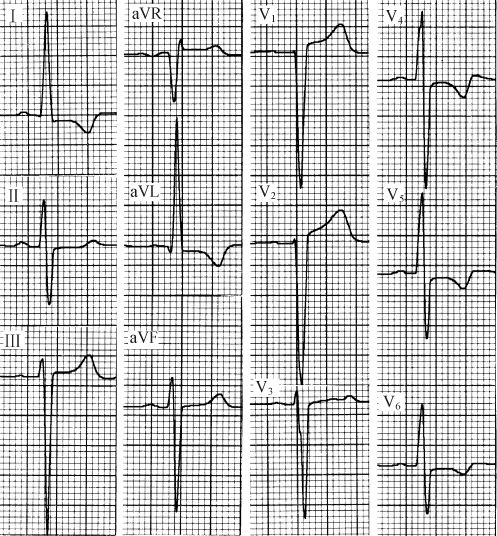
\includegraphics[width=3.22917in,height=2.21875in]{./images/Image00053.jpg}
\end{table}

当确认患者是上消化道出血后,需要迅速对下列问题作出判断,以便及时采取相应的处理。

\subsubsection{出血严重程度的估计和周围循环状态的判断}

对制定合理的治疗方案极为重要。

\paragraph{失血量的判断与临床分级}

上消化道出血病情严重度与失血量呈正相关。一般而言,粪便隐血试验阳性提示每日失血量在5ml以上;出现黑粪者,每日出血量在50~70ml以上;如短期内出血量在250~300ml,多可导致呕血。因呕血与黑便混有胃内容物与粪便,而部分血液贮留在胃肠道内未排出,故难以根据呕血或黑便量精确判断出血量。常根据临床综合指标判断失血量的多寡,对出血量判断通常分为:大量出血(急性循环衰竭,需输血纠正者。一般出血量在1000ml以上或血容量减少20\%以上)、显性出血(呕血或黑便,不伴循环衰竭)和隐性出血(粪隐血试验阳性)。临床可以根据血容量减少导致周围循环的改变(伴随症状、脉搏和血压、化验检查)来判断失血量,并根据患者年龄、有无伴发病、失血量等指标将上消化道出血严重程度分为轻、中、重度三级(表\ref{tab13-2})。

\paragraph{体位倾斜试验}

方法为先测平卧位时的血压(V\textsubscript{0}
)、脉搏(P\textsubscript{0}
),改为半卧位3分钟后,再测血压(V\textsubscript{1}
)、脉搏(P\textsubscript{1}
),符合下列条件之一者,提示失血量在1000ml以上。①V\textsubscript{0} −
V\textsubscript{1} >10mmHg;②P\textsubscript{1} − P\textsubscript{0} >
20次/分;③改半卧位后出现头晕、晕厥。必须在输液通路建立后才能进行,休克者禁作此试验。

\paragraph{休克指数}

为脉搏(次/分)与收缩压(mmHg)的比值(P/SBP),指数正常值约为0.58。指数为1.0,大约失血800~1200ml(占血容量20\%~30\%);指数大于1.0,失血量1200~2000ml(占血容量30\%~50\%)。

\paragraph{Hb、RBC和Hct的测定}

是估计失血量及决定输血量的重要参考指标。但在急性失血早期,由于血液浓缩及血液重新分布等代偿机制,上述指标可暂时无变化。一般出血3~4小时后,组织液渗入血管内补充血容量,患者可出现贫血,约24~72小时左右Hb稀释到最大限度。在连续测定中,三者迅速下降,表示继续出血,经输血纠正血容量后,与出血前比较,Hb每下降10g/L提示失血容量约400ml。

应指出的是,急性大出血严重程度的估计最有价值的指标是血容量减少所导致周围循环衰竭的临床表现,而周围循环衰竭又是急性大出血导致死亡的直接原因。因此,对急性消化道大出血患者,应将对周围循环状态的有关检查放在首位,并据此作出相应的紧急处理。血压和心率是关键指标,需进行动态观察,综合其他相关指标加以判断。如患者体位倾斜试验阳性,则提示血容量明显不足,是紧急输血的指征。如收缩压<
90mmHg,HR >
120次/分,伴有面色苍白,四肢湿冷,烦躁不安或神志不清则已进入休克状态,属严重大量出血(指3小时内需输血1500ml才能纠正其休克),需积极抢救。

\begin{table}[htbp]
\centering
\caption{上消化道出血病情严重程度分级}
\label{tab13-2}
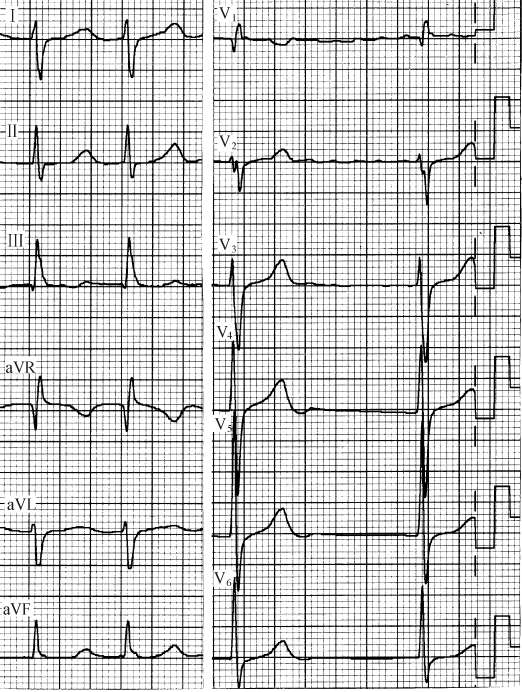
\includegraphics[width=6.65625in,height=0.91667in]{./images/Image00054.jpg}
\end{table}

\subsubsection{出血是否停止的判断}

临床上不能单凭Hb在下降或大便柏油样来判断出血是否停止或持续。因为一次出血后,Hb的下降有一定过程;而一次出血后柏油样大便持续天数受患者排便次数及出血量的影响。如每日排便1次,出血量在1000ml左右者,柏油样大便可持续1~3天,隐血试验阳性可达1周;若出血量在2000ml左右,柏油样大便可持续4~5天,隐血试验阳性达2周。应综合分析,特别是血压与脉搏的反复测定,直至恢复正常并趋稳定,尿量足(>
30ml/h),患者一般情况明显恢复者,方可认为已无活动性出血。有下列表现者,应认为有持续出血或再出血:①反复呕血或柏油样便次数及量增多,质稀薄,甚至排出暗红或鲜红色血便,伴肠鸣音活跃。②胃管抽出物有较多新鲜血。③周围循环衰竭的表现经积极补充血容量仍未见明显改善,或曾一度好转又很快恶化,中心静脉压仍有波动,稍稳定又再下降。④在补液量和排尿量足够的情况下,原无肾脏病变患者的BUN持续或再次升高。⑤Hb、RBC和Hct持续下降,血中网织红细胞持续增高。

肝硬化门静脉高压食管胃静脉曲张出血的防治共识(2008,杭州)关于EGVB继续出血或再出血的评估:①提示EGVB出血未控制的征象:72小时内出现以下表现之一者为继续出血。6小时内输血4个单位以上,生命体征不稳定。收缩压<
70mmHg,HR > 100次/分或心率增加> 20
次/分;间断呕血或便血,收缩压降低20mmHg以上或心率增加>
20次/分,继续输血才能维持Hb含量稳定;药物或内镜治疗后新鲜呕血,在没有输血的情况下,Hb含量下降30g/L以上。②提示EGVB再出血的征象:出现以下表现之一者为再出血。出血控制后再次有活动性出血的表现(呕血或便血;收缩压降低20mmHg以上或心率增加>
20
次/分;在没有输血的情况下,Hb含量下降30g/L以上)。早期再出血:出血控制后72小时~6周内出现活动性出血。迟发性再出血:出血控制6周后出现活动性出血。

\subsubsection{出血的病因诊断}

对上消化道大出血的患者,应首先纠正休克,然后尽快查找出血的部位与病因,以决定进一步的治疗措施和判断预后。一般通过询问病史、体检和必要的辅助检查,可明确出血的病因。

\paragraph{病史与体检}

详询病史和系统体检,仍是出血病因与部位诊断的基础。约50\%的患者可据此作出病因诊断。慢性、周期性、节律性上腹痛多提示出血来自消化性溃疡,特别是在出血前疼痛加剧,出血后减轻或缓解,更有助于消化性溃疡的诊断。有服用非甾体抗炎药等损伤胃黏膜的药物或应激状态者,可能为急性糜烂出血性胃炎。对中年以上的患者近期出现上腹痛,伴有厌食、消瘦者,应警惕胃癌的可能性。既往有病毒性肝炎、血吸虫病或酗酒病史,并有肝病与门静脉高压的临床表现,可能是食管胃底静脉曲张破裂出血。尚应注意既往有无类似出血史、诊治情况等。

\paragraph{急诊内镜检查}

急诊内镜检查是UGIB病因诊断中的首选方法。诊断正确率达80\%~94\%。急性上消化道出血的内镜检查有如下优点:①诊断正确率高:首先,内镜检查结合活检,既可明确出血部位,又可获得出血病变性质的诊断;其次,对一些上消化道钡餐检查不易发现的急性胃黏膜病变、贲门黏膜撕裂综合征、浅溃疡、胃黏膜毛细血管扩张症等,内镜可迅速作出诊断;第三,肝硬化合并上消化道出血病例,非静脉曲张破裂出血者占50\%左右,这仅能由内镜检查才能确诊。②提供预后的依据:如内镜下见溃疡基底喷血,溃疡基底血管、凝血块或红点等内镜征象可预示有再发出血的危险。③作为治疗手段:内镜诊断结合激光、高频电凝、喷洒止血剂以及给出血的曲张静脉内注射硬化剂等治疗性内镜的应用,使内镜检查不仅成为诊断工具,而且可作为止血治疗的方法。

\hypertarget{text00032.htmlux5cux23CHP1-13-1-4-4-2-1}{}
(1) NVUGIB的内镜检查:

①内镜检查能发现上消化道黏膜的病变,应尽早在出血后24~48小时内进行,并备好止血药物和器械。②内镜检查无食管胃底静脉曲张并在上消化道发现有出血病灶,NVUGIB诊断可确立。③内镜检查时根据溃疡基底特征,可用来判断病变是否稳定,凡基底有血凝块、血管显露等易于再出血。内镜检查时对出血灶病变应作Forrest分级(表\ref{tab13-3})。④应仔细检查贲门、胃底部、胃体垂直部、胃角小弯、十二指肠球部后壁及球后处,这些部位是易遗漏病变的区域。当检查至十二指肠球部未能发现出血病变者,应深插内镜至乳头部检查。发现有2个以上的病变,要判断哪个是出血性病灶。⑤有内镜检查禁忌证者不宜作此检查:如心率>
120次/分,收缩压< 90mmHg或较基础收缩压降低> 30mmHg、血红蛋白<
50g/L等,应先迅速纠正循环衰竭,血红蛋白上升至70g/L后再行检查。危重患者内镜检查时应进行血氧饱和度和心电、血压监护。

\begin{table}[htbp]
\centering
\caption{出血性消化性溃疡的 Forrest分级}
\label{tab13-3}
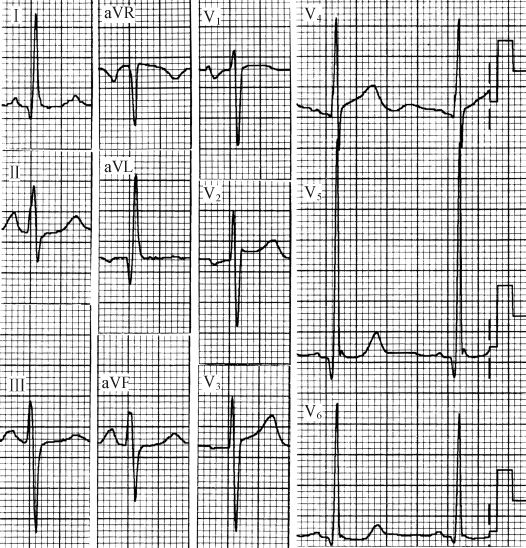
\includegraphics[width=3.26042in,height=1.5in]{./images/Image00055.jpg}
\end{table}

\hypertarget{text00032.htmlux5cux23CHP1-13-1-4-4-2-2}{}
(2) EGVB的内镜检查:

①内镜检查见有食管或胃曲张静脉出血,EGVB诊断即可成立;内镜检查时发现粗大曲张静脉和胃内血液而无其他可以识别的出血原因,EGVB诊断也可成立。②按食管静脉曲张形态及出血危险程度可将食管静脉曲张分轻、中、重3级。轻度(G\textsubscript{1}
):食管静脉曲张呈直线形或略有迂曲,无红色征(曲张静脉表面红斑、红色条纹和血疱)。中度(G\textsubscript{2}
):食管静脉曲张呈直线形或略有迂曲,有红色征或食管静脉曲张呈蛇形迂曲隆起但无红色征。重度(G\textsubscript{3}
):食管静脉曲张呈蛇形迂曲隆起且有红色征或食管静脉曲张呈串珠状、结节状或瘤状(不论是否有红色征)。③有内镜检查禁忌证者不宜作此检查(见前述)。

\hypertarget{text00032.htmlux5cux23CHP1-13-1-4-4-2-3}{}
(3) 内镜阴性患者的病因检查:

①仍有活动性出血的患者,应急诊行选择性腹腔动脉或肠系膜动脉造影,以明确出血部位和病因,必要时同时作栓塞止血治疗。②在出血停止,病情稳定后可作胃肠钡剂造影或放射性核素扫描(如\textsuperscript{99m}
锝标记患者的红细胞),但此检查特异性差。③对慢性隐性出血或少量出血者,可考虑作小肠镜检查。④对经各种检查仍未能明确诊断而出血不停者,病情紧急时可考虑剖腹探查,可在术中结合内镜检查,明确出血部位。

\paragraph{X线钡餐检查}

目前已多为胃镜检查所替代。消化道大出血患者,因休克不能站立和充分变换体位,胃内潴留大量血液或血块影响钡餐充盈和病变征象观察,不易显示某些浅表病变如胃炎、急性胃黏膜病变等,仅能发现病变而不能确定是否为出血病变等,还可干扰以后内镜检查和血管造影检查,以及在活动性出血时,过早进行此项检查有加重出血的危险等因素,使急诊X线钡餐检查的实用性大大受到限制。因此,上消化道钡餐检查仅适用于出血已停止、生命体征平稳的上消化道出血患者。但对经胃镜检查出血原因未明、疑病变在十二指肠降段以下小肠段,则有特殊诊断价值。对某些解剖部位的改变,如胃黏膜脱垂、食管裂孔疝的诊断却优于一般胃镜检查。一般宜在出血完全停止3天后谨慎进行。

\paragraph{血管造影}

对内镜检查无阳性发现或不适宜进行内镜检查者如有严重的心、肺并发症,且仍有活动性出血的患者可做选择性血管造影,对肠血管畸形、小肠平滑肌瘤等有很高的诊断价值,并可同时进行介入治疗。但忌用于严重动脉硬化、对碘剂过敏和老年患者。该检查的优点是:①灵敏性强:实验证明,出血量在0.5ml/min以上的消化道出血,在选择性血管造影连续摄影中即可见到造影剂从破裂血管外溢的X线征象。对慢性、隐源性活动性消化道出血是一种极有价值的诊断方法,阳性率一般为77\%~90\%。一般选择肠系膜上动脉及腹腔动脉造影已足够显示所要的范围。②具有精确的出血定位诊断价值:经出血相关区域血管注射造影剂,可精确显示出血部位和出血病变的供应动脉,为确定治疗提供了精确的解剖依据。③消化道内积血或血块不影响血管造影剂外溢的X线征象观察。④出血部位及其供应动脉显示后,立即经血管造影导管注射血管收缩剂或血管栓塞剂进行止血治疗。此外,门静脉造影(包括经脾穿刺门静脉造影、经肝穿刺门静脉造影以及经脐静脉插管门静脉造影等)除可以显示血管破裂部位、进行栓塞治疗外,还可以经导管测量门静脉压力诊断门脉高压症。

\paragraph{放射性核素扫描}

经内镜及X线检查阴性的病例,可做放射性核素扫描。方法是采用核素(如\textsuperscript{99m}
锝)标记患者的红细胞后,再从静脉注入患者体内,当有活动性出血,且出血速度达到0.1ml/min,核素便可显示出血部位。注射一次\textsuperscript{99m}
锝标记的红细胞,可以监视患者消化道出血达24小时。本法缺点为出血部位定位不够确切,也不能确定出血病变的性质。

\subsubsection{预后估计与危险性分级}

约80\%~85\%急性上消化道出血患者除支持疗法外,无需特殊治疗出血可在短期内自然停止。仅有15\%~20\%患者持续出血或反复出血,而主要是这类患者由于出血并发症而导致死亡。如何早期识别再出血及死亡危险性高的患者,并给予加强监护和积极治疗,便成为急性上消化道出血处理的重点。提示预后不良、危险性增高的主要因素有:①高龄患者(>
60岁);②有严重伴随病(心、肺、肝、肾功能不全,脑卒中等);③本次出血量大或短期内反复出血;④特殊病因和部位的出血(如食管胃底静脉曲张破裂出血);⑤消化性溃疡伴有内镜下活动性出血,或近期出血征象。此外,EGVB出血48小时内肝静脉压力梯度(HVPG)>
20mmHg是其可靠的预后不良预测因子。

Rockall评分系统(表\ref{tab13-4}\footnote{\textsuperscript{※} 收缩压> 100mmHg,心率<
100次/分;\textsuperscript{△} 收缩压> 100mmHg,心率>
100次/分;\textsuperscript{▲} 收缩压< 100mmHg,心率> 100次/分})仍是目前临床广泛使用的评分依据,该系统依据患者年龄、休克状况、伴发病、内镜诊断和内镜下出血征象5项指标,将UGIB患者分为高危、中危或低危三级,积分≥5分者为高危,3~4分为中危,0~2分为低危。在Rockall评分系统中,若仅根据年龄、休克表现及伴发病三个指标评判疾病危险度,谓之为临床Rockall评分系统,可适用于无条件获取急诊内镜资料的基层医院;若同时有急诊内镜资料参与评估,谓之为完全Rockall评分系统。如出血患者,61岁,收缩压为105mmHg,心率为110次/分,胃镜下可见一巨大溃疡,活检示胃腺癌,附血凝块,无伴发病。则该患者Rockall积分=年龄(1)+心动过速(1)+无伴发病(0)+胃癌(2)+近期出血征象(2)=
6分,为高危患者。

Blatchford评分系统(表\ref{tab13-5}\footnote{积分≥6分为中高危,< 6分为低危;1mmHg = 0.133kPa})包含了BUN、Hb等实验室检查信息,其价值逐渐得到认可。

\begin{table}[htbp]
\centering
\caption{急性 UGIB患者的Rockall再出血和死亡危险性评分系统}
\label{tab13-4}
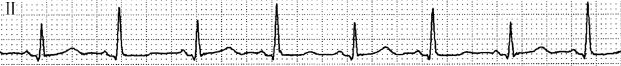
\includegraphics[width=6.67708in,height=1.83333in]{./images/Image00056.jpg}
\end{table}

\begin{table}[htbp]
\centering
\caption{急性上消化道出血患者的 Blatchford评分}
\label{tab13-5}
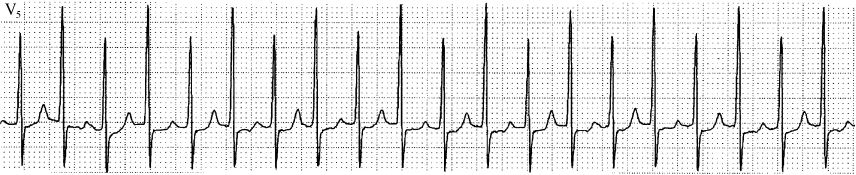
\includegraphics[width=3.32292in,height=3.75in]{./images/Image00057.jpg}
\end{table}

\subsection{处理原则}

及早补充血容量、防治继续出血和再出血及病因治疗。其中,抗休克、迅速补充血容量应放在一切医疗措施的首位。

关于UGIB诊治流程,中国医师协会急诊医师分会制定的《急性上消化道出血急诊诊治专家共识》将上消化道出血的急诊诊治过程分为三个阶段,分别是紧急治疗期、病因诊断期和加强治疗期。紧急治疗期:患者入院6~48小时,治疗目标是控制急性出血、维持患者生命体征平稳并针对患者病情做出初步诊断及评估,治疗手段以药物治疗为主(PPI、生长抑素和抗菌药物联合用药)。病因诊断期:入院48小时内,急性出血得到控制,患者血流动力学稳定的情况下,行急诊内镜检查以明确病因并进行相应的内镜下治疗。无法行内镜检查的患者,可根据情况进行经验性诊断、评估和治疗。加强治疗期:入院后3~7天,治疗目标是病因治疗,预防早期再出血的发生。病因明确后,可根据不同病因采取不同的治疗手段。临床推荐采用以药物联合内镜治疗为主的综合治疗方法。

\subsubsection{一般措施}

患者应取平卧位休息,吸氧,严密观察患者的神色、血压、脉搏、出血量和尿量;保持静脉通道通畅,必要时作静脉切开。保持呼吸道通畅,避免呕血时引起窒息。烦躁不安者可给予镇静剂,如地西泮(安定)10mg肌注,对肝病患者忌用巴比妥类药物。呕血者宜暂禁食,但少量出血者宜进流质(因为胃内空虚产生饥饿的不正常的胃收缩不利于止血),活动性出血停止后可逐渐改变饮食的质与量。推荐对活动性出血或大出血患者宜常规放置胃管,其意义有:①可以观察出血情况,并可用冰盐水洗胃止血;②抽取胃内容物,减轻胃扩张,改善胃黏膜的循环,抽出积存在胃内的血液,能减轻日后吸收热和氮质血症,降低胃内酸度,防止凝血块被消化,有利于止血;③可通过胃管及时用药治疗;④预防吸入性肺炎;⑤鼻饲营养液。意识障碍和排尿困难者需留置尿管,危重大出血者必要时进行中心静脉压测定,老年患者常需心电、血氧饱和度、呼吸监护。

\subsubsection{迅速补充血容量}

迅速补充血容量是处理上消化道大出血的首要措施。立即查血型和配血,尽快建立有效的静脉输液通道,尽快补充血容量。在配血过程中,可先输平衡液或葡萄糖盐水。失血量较大(如减少20\%血容量以上)时,可输入血浆等胶体扩容剂。改善急性失血性周围循环衰竭的关键是要输血,一般输浓缩红细胞,严重活动性大出血考虑输全血。下列情况为紧急输血指征:①收缩压<
90mmHg(EGVB时< 80mmHg),或较基础收缩压降低幅度> 30mmHg;②Hb <
50~70g/L(EGVB时Hb < 50g/L),Hct < 25\%;③心率增快(>
120次/分)。输血量依失血量而定,原则上输血量应接近出血量。输血注意事项:①输血开始时,速度应加快,以尽快把收缩压升高至80~90mmHg水平,待血压稳定、病情改善后则减慢输血、输液速度,避免依赖升压药来维持血压。②避免输血、输液过多、过快,招致急性肺水肿,尤其是对有心、肺、肾疾患及老年患者。③防止枸橼酸中毒,一般每输血600~900ml可从静脉注入10\%葡萄糖酸钙10ml,以防低钙。④大量输注库存血时易引起高钾血症,应注意给予高渗葡萄糖,必要时加用适量胰岛素。⑤对肝硬化门脉高压静脉曲张破裂出血时,应输新鲜全血,除恢复血容量外,尚因其含有多种凝血因子和血小板成分,对止血有益;还可避免输库存血(含氨多)过多诱发肝性脑病。另外,输入的血约为失血量的2/3或3/4,以避免门静脉压力增高致再出血的危险。对于EGVB,以维持血流动力学稳定并使Hb维持在80g/L以上;过度输血或输液可能导致继续或重新出血;避免仅用氯化钠溶液补足液体,以免加重或加速腹水或其他血管外液体的蓄积;必要时应及时补充凝血因子、凝血酶原复合物等;血小板<
50 × 10\textsuperscript{9}
/L者,可输注血小板。对于急性大量出血者,应尽可能施行中心静脉导管置管和中心静脉压监测,以指导液体复苏。在补足液体的前提下,如血压仍不稳定,可以适当地选用血管活性药物(如多巴胺)以改善重要脏器的血液灌注。血容量充足的指征:①神志清楚或好转,无明显脱水貌;②收缩压90~120mmHg;③脉搏<
100次/分;④尿量> 40ml/h,血钠< 140mmol/L。

\subsubsection{非静脉曲张性上消化道出血(nonvariceal UGIB,NVUGIB)的止血措施}

NVUGIB是指除食管胃底静脉曲张破裂出血以外的其他病因引起的上消化道出血。包括消化性溃疡、急性糜烂出血性胃炎、胃泌素瘤、食管裂孔疝等所致的出血。止血措施主要有:

\paragraph{内镜下止血}

起效迅速、疗效确切,应作为首选。可根据医院的设备和病变的性质选用,常用方法有:

\hypertarget{text00032.htmlux5cux23CHP1-13-1-5-3-1-1}{}
(1) 对出血灶喷洒止血药物:

内镜下直接对出血灶喷洒止血药物,对局部渗血疗效较好,对动脉性出血疗效较差。常用的药物有去甲肾上腺素溶液、孟氏液、注射用血凝酶、凝血酶等。

\hypertarget{text00032.htmlux5cux23CHP1-13-1-5-3-1-2}{}
(2) 局部注射法:

当内镜检查发现喷射性出血或血管显露时,可用局部注射法止血。常用的注射剂有肾上腺素溶液、凝血酶、无水酒精、高渗盐水等。其方法是在出血血管周围1~2mm处选3~4点,每点注入0.1~0.3ml。本法安全、有效,且可反复应用。

\hypertarget{text00032.htmlux5cux23CHP1-13-1-5-3-1-3}{}
(3) 激光照射法:

可供止血的激光有氩激光(Argon)和镱-铝-石榴石激光(Nd-YAG)两种。后者功率大,止血效果好。止血机制是由于光凝作用,使照射局部组织蛋白凝固,小血管内血栓形成。止血成功率在80\%~90\%。其并发症有胃肠穿孔、出血及胃肠胀气等。

\hypertarget{text00032.htmlux5cux23CHP1-13-1-5-3-1-4}{}
(4) 微波凝固法:

将微波经内镜导入出血部位,使产生热凝固,达到止血目的。其优点是,操作简便,并可将微波针状电极直接插入组织内治疗,插入组织的深度易控制,因而止血目标确切,安全性大。

\hypertarget{text00032.htmlux5cux23CHP1-13-1-5-3-1-5}{}
(5) 高频电凝止血法:

应用高频电流的热效应,使局部组织蛋白变性达到止血,迅速止血率达87\%~96\%。主要用于血管显露性出血及有直接出血征象的出血性病变。方法是用凝固电流在出血灶周围电凝,使黏膜下层或肌层的血管凝缩,最后电凝出血血管。有出血、溃疡、穿孔等并发症。近年来为了提高电凝止血的安全性和止血效果,研制出各种形状的及带喷水孔的单极电凝头、双极电凝头及四头双极电凝探头。

\hypertarget{text00032.htmlux5cux23CHP1-13-1-5-3-1-6}{}
(6) 热探头凝固法:

是利用热探头的高温(150℃)接触出血灶,使其组织蛋白质凝固而达到止血。此法疗效确切、安全、简单。

\hypertarget{text00032.htmlux5cux23CHP1-13-1-5-3-1-7}{}
(7) 放置止血夹法:

内镜直视下放置止血夹子,把出血的血管夹住止血,伤口愈合后此金属夹子自行脱落随粪便排出体外,此法止血既安全又有效。适用于消化性溃疡、急性胃黏膜病变的出血治疗,尤其在小动脉出血时用该法甚佳。

\paragraph{制酸药物的应用}

胃酸在上消化道出血中起重要作用,抑制胃酸分泌及中和胃酸可达到止血的效果。制酸药止血的关键是使胃内pH维持在>
6,这样,既可促进血小板聚集和纤维蛋白凝块的形成,避免血凝块过早溶解,有利于止血和预防再出血,又可治疗消化性溃疡等病变。尤适用于消化性溃疡、急性胃黏膜病变、胃泌素瘤、食管裂孔疝等所致的出血。常用制剂有:

\hypertarget{text00032.htmlux5cux23CHP1-13-1-5-3-2-1}{}
(1) 中和胃酸药:

将胃内容物抽尽,用氢氧化铝凝胶60ml经胃管注入,15分钟后测胃液pH,若<
6,再注入60ml,以后每小时测pH1次,使其值维持在> 6。

\hypertarget{text00032.htmlux5cux23CHP1-13-1-5-3-2-2}{}
(2) H\textsubscript{2} 受体阻滞剂(H\textsubscript{2} RA):

目前临床上常用的有:第一代的西咪替丁(cimetidine,甲氰咪胍)、第二代的雷尼替丁(ranitidine)和第三代的法莫替丁(famotidine)。由于后两者不仅抗酸作用强(雷尼替丁比西咪替丁强5~8倍,法莫替丁比西咪替丁强30~100倍),作用时间更持久,且毒副作用相对较轻,应作为首选。可用雷尼替丁50mg缓慢静脉注射,每6~12小时1次,或用150~300mg加入液体中持续静滴;法莫替丁20mg溶入生理盐水或葡萄糖液20ml中,缓慢静脉注射,每日2次。

\hypertarget{text00032.htmlux5cux23CHP1-13-1-5-3-2-3}{}
(3) 质子泵抑制剂(proton pump inhibition,PPI):

可抑制胃壁细胞的H\textsuperscript{+} -K\textsuperscript{+}
-ATP酶,从而抑制胃酸的分泌。其抑制胃酸作用远强于H\textsubscript{2}
RA,几乎完全抑制酸分泌,持续用药无耐受性,且作用持久、递增,3~5天达稳态,胃内pH维持平稳。大剂量PPI可减少高危患者再出血率,且总费用降低,是治疗NVUGIB的首选止血药物。加拿大NVUGIB共识会议推荐内镜止血成功后应用PPI,在待行内镜检查时也应给予大剂量PPI,并认为H\textsubscript{2}
RA不能减少再出血率及病死率,不提倡用H\textsubscript{2}
RA止血。PPI常用制剂有:奥美拉唑(omeprazole,又名洛赛克,Losec)、泮托拉唑(pantoprazole)和兰索拉唑(lansoprazole)等。PPI给药方法及剂量:高危患者应静脉给药,如奥美拉唑静脉推注80mg后,以8mg/h输注72小时;如低危患者可口服给药,如奥美拉唑20mg,每6小时一次,持续5天。

\paragraph{奥曲肽(octreotide)}

商品名善得定(Sandostatin),是人工合成的生长抑素类似品。能抑制胃酸、胃蛋白酶和胃泌素分泌,促进胃黏膜生长,能选择性引起内脏循环血流量减少和门脉压下降。用法:100μg皮下注射,每日2~4次。

\paragraph{去甲肾上腺素}

可使胃肠黏膜出血区域的小动脉强烈收缩,减少局部血流量,并能减少胃酸分泌,有类似迷走神经切断的作用;同时因可降低门脉压,故亦用于食管静脉曲张破裂出血。用法有二:①口服或胃管内灌入:用去甲肾上腺素8mg加入冷生理盐水100~200ml中为1次量,口服或由胃管内灌入,每0.5小时1次,共2~4次;若有效,可再改为1小时1次,共4~6小时,以后每2小时1次共4~6小时。若无效,则不用。②腹腔灌注:以细长穿刺针作腹腔穿刺,注入含去甲肾上腺素8mg的生理盐水100ml,然后来回转动患者腹部,出血可迅速停止。本法适用于有腹水者,以免注入组织内引起缺血性坏死。

\paragraph{注射用血凝酶(立止血,reptilase)}

是酸性止血剂,含有如凝血激酶和凝血酶样物质,可直接作用于内、外源性凝血系统形成凝血活酶,促进凝血酶的形成而起到凝血作用。用法:首次静注与肌注各1kU,继而每日肌注1kU。无明显毒副作用。

\paragraph{凝血酶(thrombin)}

本品是从猪血提取、精制而得的凝血酶无菌制剂。能直接作用于出血部位的纤维蛋白原,使其转变为纤维蛋白,促使血液凝固、填塞出血点而止血;尚有促进上皮细胞的有丝分裂而加速创伤愈合的作用。其特点是局部止血迅速,疗效显著,无明显不良反应,但出现过敏反应时,应立即停用。首次剂量宜大(8000U~2万U),溶入50~100ml生理盐水或牛奶、豆汁内口服或胃管内注入,每2~6小时1次,应用次数视病情而定。凝血酶遇热或在酸性环境中均易失去活性,故溶液温度不要超过37℃,同时给予抑酸药物(如H\textsubscript{2}
受体阻滞剂、质子泵抑制剂)以便得以发挥最大作用。本品切忌血管内或肌内注射。

\paragraph{其他止血药物}

以下止血药物对NVUGIB的确切效果未能证实,不作为一线药物使用。应避免滥用止血药。可酌情选用的有:①维生素K:能促进凝血酶原及凝血因子Ⅷ、Ⅵ、Ⅳ、Ⅹ在肝内合成。可用维生素K\textsubscript{1}
10mg肌注,每日2次;或维生素K\textsubscript{4}
口服4mg,每日3次;②肾上腺色腙(安络血):可增强受损毛细血管的修复能力,从而达到止血目的。10mg肌注,每天2次;或5~10mg口服,每天3~4次。③酚磺乙胺(止血敏):有增强血小板的作用。0.5~1.0g口服,每天3次;或0.5g肌注或静注。④氨甲苯酸(止血芳酸)、氨基己酸:能抑制纤溶酶原的激活因子和抑制纤维蛋白的溶解。⑤中药:云南白药、三七粉、白及粉、血余炭等均有防腐生肌、凉血止血的作用,中成药如止血散(白及、煅瓦楞、三七、甘草)、止血粉(白及、蒲黄、地榆、甘草)、止血汤(仙鹤草、地榆炭、白及、生槐花)等可酌情辨证选用。

\paragraph{选择性血管造影及栓塞治疗}

选择性胃左动脉、胃十二指肠动脉、脾动脉或胰十二指肠动脉血管造影,针对造影剂外溢或病变部位经血管导管滴注血管升压素或去甲肾上腺素,导致小动脉和毛细血管收缩,使出血停止。无效者可用明胶海绵栓塞。

\paragraph{手术治疗}

诊断明确但药物和介入治疗无效者,诊断不明确、但无禁忌证者,可考虑手术,结合术中内镜止血治疗。约10\%的胃十二指肠溃疡大出血患者需急症手术止血,手术指征为:①出血速度快,短期内发生休克,或较短时间内(6~8小时)需要输入较大量血液(>
800ml)方能维持血压和Hct者;②年龄在60岁以上伴动脉硬化症者自行止血机会较小,对再出血耐受性差,应及早手术;③近期发生过类似的大出血或合并穿孔或幽门梗阻;④正在进行药物治疗的胃十二指肠溃疡患者发生大出血,表明溃疡侵蚀性大,非手术治疗难以止血;⑤内镜检查发现动脉搏动性出血,或溃疡底部血管显露再出血危险很大。急诊手术应争取在出血48小时内进行,胃溃疡较十二指肠溃疡再出血概率高3倍,应争取及早手术。

\paragraph{原发病的治疗}

对出血的病因比较明确者,如幽门螺杆菌阳性的消化性溃疡患者,应予抗幽门螺杆菌治疗及抗溃疡治疗。需要长期服用非甾体抗炎药者一般推荐同时服用PPI或黏膜保护剂。

非静脉曲张性上消化道出血诊治流程见图\ref{fig13-1}。

\subsubsection{食管胃静脉曲张出血的止血治疗}

肝硬化门脉高压症患者发生上消化道出血,并不全是由食管胃底静脉曲张破裂所致,而是多种因素共同作用的结果。因此,它的治疗仍应以上述治疗措施为基础。EGVB活动性出血的止血措施主要有内镜治疗、血管活性药物、经颈静脉肝内门体分流术(transjugular
intrahepatic portosystemic
shunt,TIPS)、外科手术和双气囊堵塞压迫等。其作用机制、运用方法及注意事项等有关内容,详见本书第116章第1节“肝硬化并上消化道出血”部分。

\subsubsection{预后}

据临床资料统计,约80\%~85\%急性上消化道大量出血的患者除支持疗法外,无需特殊治疗,出血可在短期内自然停止。仅有15\%~20\%患者持续出血或反复出血,常因出血并发症而导致死亡。如何早期识别再出血及死亡危险性高的患者,并予加强监护和积极治疗,便成为急性上消化道大量出血处理的重点。提示预后不良危险性增高的主要因素有:①高龄患者(>
60岁);②有严重伴随病(心、肺、肝、肾功能不全、脑卒中等);③本次出血量大或短期内反复出血;④特殊病因和部位的出血(如食管胃底静脉曲张破裂出血);⑤消化性溃疡伴有内镜下活动性出血,或近期出血征象。

\begin{figure}[!htbp]
 \centering
 \includegraphics[width=4.23958in,height=3.55208in]{./images/Image00058.jpg}
 \captionsetup{justification=centering}
 \caption{急性非静脉曲张性上消化道出血诊治流程}
 \label{fig13-1}
  \end{figure} 

PPIs:质子泵抑制剂;H\textsubscript{2} RA:H\textsubscript{2} 受体拮抗剂

\protect\hypertarget{text00033.html}{}{}

\section{下消化道出血}

下消化道出血(lower gastrointestinal
hemorrhage)是指屈氏韧带以下的小肠或大肠出血。依其出血量大小、速度和快慢等可分为三类:①慢性隐性出血:肉眼不能观察到便血,仅有大便隐血试验阳性,常以不明原因贫血就诊或普查时发现。②慢性少量显性出血(亚急性出血):表现为间歇性或持续性肉眼可见的少量显性便血,可呈鲜红色、果酱样或柏油样黑粪,无循环衰竭表现。③急性大量出血:短期内排出大量鲜红或暗红色血便,伴血压下降等休克症状,常需输血治疗者。多数下消化道出血相对缓慢,或呈间歇型,约80\%的出血能自行停止。在治疗上除了止血、补充血容量以外,寻找下消化道出血部位、疾病性质进行原发病病因治疗最为重要。

下消化道范围广,出血病因繁多,分类各异。如按病变部位可分为:①小肠疾病:小肠肿瘤、黑色素-胃肠息肉综合征、克罗恩病(Crohn病)、小肠憩室与Meckel憩室、肠套叠、小肠血管畸形、急性出血性坏死性肠炎、缺血性小肠炎和肠结核等。②大肠疾病:溃疡性结肠炎、结肠息肉、结肠憩室、菌痢、阿米巴痢疾、结肠癌、克罗恩病、缺血性结肠炎、结肠子宫内膜异位症、结肠结核及肠套叠、结肠血管畸形等。③直肠疾病:直肠溃疡、非特异性炎症、肿瘤、息肉、放射性直肠炎和腹盆腔邻近脏器恶性肿瘤或脓肿侵及直肠等。④肛管疾病:痔、肛裂、肛瘘。此外,还有全身性疾病累及肠道。国内资料引起下消化道出血的最常见病因为大肠癌和大肠息肉,其次为肠道炎症性疾病(其中肠伤寒、肠结核、溃疡性结肠炎、克罗恩病和坏死性小肠炎有时可发生大量出血)和血管病变,憩室引起的出血少见。但在西方国家,血管病变和消化道憩室是下消化道出血最常见病因,其次为结肠肿瘤和炎症性肠病。

\subsection{诊断思路}

\paragraph{下消化道出血的确立}

首先要排除口腔、鼻咽、喉、气管、支气管、肺等部位的出血被吞咽后由肛门排出的可能性,还要与下列情况区别:①口服某些中草药、兽炭、铁剂、铋剂时,大便可呈暗褐色或黑色,但隐血试验阴性;②食用过多的肉类、猪肝、动物血后大便可变暗褐色,隐血试验呈阳性,但素食后即转呈阴性;③口服酚酞制剂,大便有时呈鲜红色,不注意时易误诊为大量便血。

排除了上述因素后,要确定是否为下消化道出血,大便的色泽和量是重要的线索,通常大便呈鲜红色或暗红色者,即可确诊。但如为暗红色大量血便或仅表现为黑便或大便隐血阳性时,则应与上消化道出血鉴别。此时应常规行胃十二指肠镜检查,若未发现病变,大致可除外上消化道出血。

下述几点有助于下消化道出血的诊断:①病史中多伴有下腹痛或腹部有包块,排便异常伴便血史,出血前常有中下腹不适、下坠或便意。②大便常为鲜红、暗红、果酱样,少数为黑便,无呕血。③下消化道出血时胃管内无咖啡色的液体和暗红色的血液被抽出。④来自高位小肠的出血可能有血BUN升高,而结肠出血常不升高;上消化道出血时血BUN升高较下消化道出血时明显。⑤结直肠出血,常表现为鲜血便或是暗红的血便,血与大便相混,可有便后滴血,亦可表现为脓血便。⑥小肠出血常为暗红果酱样便,亦可为黑便,偶有血水样便。⑦大肠出血常伴有下腹痛、腹泻、里急后重等症状,而小肠出血常表现为脐周疼痛。

\paragraph{估计出血速度和出血量}

下消化道出血确定后,估计出血速度和出血量甚为重要。判断患者出血速度和出血量的最终标准取决于为恢复和维持血容量所需的输血量和速度。在此之前,则可根据有无循环障碍及其程度、Hct和Hb变化作出初步估计。

\paragraph{确定是否由全身性疾病所致下消化道出血}

全身性疾病所致的下消化道出血有相应疾病的全身表现。血液系疾病、血管疾病、肝脏疾病和某些中毒性疾病常伴有凝血与止血功能障碍,有凝血因子缺乏、血小板质或量改变、血管脆性增加、血管收缩障碍的实验室发现。相反,多数传染性疾病及中毒性疾病下消化道出血的主要原因是肠黏膜、黏膜下血管受损的后果。血液检查、骨髓检查、凝血机制检查等有助于诊断。

\paragraph{出血部位的判断}

下消化道出血最常见的部位是乙状结肠,占50\%左右。其他部位出血频率依次为直肠、降结肠、横结肠、升结肠、盲肠、小肠。根据出血类型常可对出血部位作出初步判断:仅大便隐血阳性者,若排除了上消化道出血,则多为右侧结肠和小肠出血;少量显性出血,则主要是结肠、直肠出血;鲜红或暗红色血便,以左半结肠和直肠为主;果酱色或咖啡色血便则多为右半结肠出血。虽右半结肠和小肠出血的发生率较低,但较易发生急性大出血。上位结肠出血时,血与大便常混杂;乙状结肠和直肠出血时,常有新鲜血液附着于成形大便的表面。血在大便后滴下,与粪便不相混杂者,虽多见于内痔、肛裂,但也可见于直肠息肉和直肠癌,应予以注意。

\paragraph{出血病因的诊断}

病史与体检是出血病因诊断中最重要的基础工作。

\hypertarget{text00033.htmlux5cux23CHP1-13-2-1-5-1}{}
(1) 既往史:

①反复小量显性出血史,提示痔、息肉、憩室等。②大便习惯改变或大便变细有切迹,应警惕结肠、直肠肿瘤。③反复血性腹泻史提示炎症性肠病可能。④曾患疾病与用药:曾患肺结核者应考虑肠结核;动脉硬化、心律失常、口服避孕药者应考虑缺血性结肠炎;风湿性疾病、白血病、出血性疾病、尿毒症、急性胰腺炎等病程中发生出血,多由于原发病引起的肠道病变;应用抗生素过程中出血应考虑假膜性肠炎、出血性结肠炎;便血前数月或数年曾接受腹部放射治疗者应考虑放射性结肠炎。

\hypertarget{text00033.htmlux5cux23CHP1-13-2-1-5-2}{}
(2) 便血特点与伴随症状:

①脓血黏液便伴里急后重或坠胀感,大便次数增多,应考虑痢疾和直肠癌可能。②中小量出血,色较红而呈间断性附于大便表面,要注意息肉出血之可能。③便血伴剧烈腹痛者,尤其是老年人心血管病患者,应警惕肠系膜血管栓塞;便血伴发热应考虑感染性肠炎、炎症性肠病、肠结核、肠伤寒、出血性坏死性肠炎、血液系疾病(白血病、恶性组织细胞病、恶性淋巴瘤等)等;便血伴腹块或不全性肠梗阻应考虑肿瘤、肠结核、Crohn病、肠套叠等;便血伴腹壁瘘管(或内瘘管),见于Crohn病、肠结核、癌、放线菌病。

\hypertarget{text00033.htmlux5cux23CHP1-13-2-1-5-3}{}
(3) 年龄与病因:

下消化道出血的病因与年龄有关:①婴儿和儿童:以Meckel憩室最多见,幼年性息肉次之,其他有炎症性肠病、肠套叠等。②青少年和成年人:在青少年时期,Meckel憩室依然是最常见病因,其次是炎症性肠病和息肉;随年龄增长癌肿比例显著增高。③老年人:以癌肿、息肉多见,其次为慢性结肠炎症、结肠血管扩张、结肠憩室等。

\hypertarget{text00033.htmlux5cux23CHP1-13-2-1-5-4}{}
(4) 出血部位与病因:

①直肠、乙状结肠:以息肉、癌、溃疡性结肠炎、单纯性溃疡、菌痢、阿米巴肠炎、放射性肠炎多见;②结肠脾曲、降结肠、乙状结肠:除息肉、癌外,易发生缺血性结肠炎;③右侧结肠:憩室、血管畸形、肠结核、Crohn病;④回盲部(回肠末段至升结肠始段):除癌、息肉外,类癌、Crohn病、单纯性溃疡、肠结核、鞭虫病、阿米巴肠炎、肠套叠、Meckel憩室、肠伤寒、沙门菌肠炎等。

\hypertarget{text00033.htmlux5cux23CHP1-13-2-1-5-5}{}
(5) 肛门视诊和直肠指检:

下消化道出血病因诊断的第一步,应采用简便易行的肛门视诊和直肠指诊,以发现或排除痔、肛裂,以及大部分直肠癌和息肉等常见的出血病因。

\hypertarget{text00033.htmlux5cux23CHP1-13-2-1-5-6}{}
(6) 内镜检查:

结肠镜检查是诊断大肠和回肠末端病变的首选检查方法。宜尽量在出血停止后近期或出血间歇期进行。对于出血灶的诊断,以窥视下直接见到活动性渗血最可靠。

\hypertarget{text00033.htmlux5cux23CHP1-13-2-1-5-7}{}
(7) X线钡剂造影检查:

一般要求在大出血停止至少3天后进行。主张双重气钡造影。其优点是基层医院已普及,患者易接受。缺点是对较平坦病变、广泛而较轻炎症性病变易漏诊,有时无法确定病变性质。对X线钡剂灌肠检查阴性的下消化道出血患者需进行结肠镜检查,已作结肠镜全结肠检查患者则不强调本项检查。

\hypertarget{text00033.htmlux5cux23CHP1-13-2-1-5-8}{}
(8) 胶囊内镜或双气囊小肠镜检查:

适用于常规内镜检查和X线钡剂造影不能确定出血来源的不明原因出血,出血活动期和静止期均可进行,可视病情和医疗条件选用。

\hypertarget{text00033.htmlux5cux23CHP1-13-2-1-5-9}{}
(9) 放射性核素扫描或选择性腹腔动脉造影:

必须在活动性出血时进行。主要用于急诊结肠镜检查不能确定出血来源的不明原因出血。放射性核素扫描检查的特点是简便敏感,出血量约0.1ml/min时即有阳性显示;缺点是对出血不能准确定位。常用本法初步确定出血部位,为进一步作血管造影提供线索。此外,利用\textsuperscript{99m}
Tc腹部扫描可用于诊断有胃黏膜异位的先天性病变,如Meckel憩室、肠重复畸形等。对持续大出血患者经上述检查不能明确出血灶时,应及时作选择性肠系膜上动脉造影,因肠系膜上动脉支配全部小肠和右侧结肠。约50\%~80\%的憩室出血和全部血管畸形出血均发生于右侧结肠。如肠系膜上动脉造影阴性,应再作肠系膜下动脉和腹腔动脉造影。血管造影可显示低至0.5ml/min的出血,此外还可显示肿瘤血管和血管畸形。成功的血管造影约于2/3的病例可显示肠出血来源。

\hypertarget{text00033.htmlux5cux23CHP1-13-2-1-5-10}{}
(10) 手术探查:

如上述检查仍不能明确出血灶,持续大出血危及患者生命,必须手术探查。术中内镜是明确诊断不明原因消化道出血,尤其是小肠出血的可靠方法。

不明原因消化道出血(obscure gastrointestinal bleeding,
OGIB)是指常规内镜检查(胃镜和结肠镜)不能确定出血来源的持续或反复消化道出血,多为小肠出血(如小肠的肿瘤、Meckel憩室和血管病变等),是消化道出血诊断的难点。OGIB的诊断步骤:在出血停止期,先行小肠钡剂检查;在出血活动期,应及时作放射性核素扫描或选择性腹腔动脉造影;若上述检查结果阴性则选择胶囊内镜或及双气囊小肠镜检查;出血不止危及患者生命者行手术探查,探查时可辅以术中内镜检查。

\subsection{处理原则}

下消化道出血主要是病因治疗,大出血时应积极抢救。

\paragraph{一般措施}

一般急救措施与补充血容量同上消化道出血一样。一般措施包括应用注射用血凝酶、静滴血管加压素、生长抑素、肾上腺色腙(安络血)、酚磺乙胺等药物。

\paragraph{局部止血措施}

对结肠出血,可给予冰盐水去甲肾上腺素液(去甲肾上腺素8mg加入100~200ml生理盐水中)、孟氏液、凝血酶等进行灌肠。

\paragraph{内镜下止血措施}

包括内镜下向出血病灶喷洒止血药物、高频电凝止血、激光止血、息肉电凝止血、黏膜和黏膜下注射硬化剂等措施止血。

\paragraph{放射性介入治疗}

在做选择性动脉造影时,若发现造影剂有渗出,即可通过导管给予血管加压素滴注,0.1~0.4U/min。对结肠出血不能自发地停止或血管加压素输注无效的病例,可施行栓塞治疗。在荧光透视下作超选择性插管,将管端插入出血灶近端几厘米处,注入明胶海绵碎片或自体凝血块,可将出血动脉栓塞、制止出血。

\paragraph{手术治疗}

经内科保守治疗仍出血不止危及生命,无论出血病变是否确诊,均是紧急手术的指征。此外,对下列情况可行手术治疗:①对Meckel憩室、肠重复畸形、恶性肿瘤、先天性动静脉畸形(包括结肠血管扩张)等皆可手术切除。②息肉病、家族性息肉病或有高度癌变倾向的息肉可手术切除。但一般息肉可经纤维结肠镜电凝切除。③溃疡性结肠炎引起的大出血是次全或全结肠切除的手术指征;Crohn病时如病变局限也可作局限性肠切除。

下消化道出血的处理程序如图\ref{fig13-2}。

\protect\hypertarget{text00034.html}{}{}

\section{不明原因消化道出血}

不明原因消化道出血(obscure gastrointestinal
bleeding,OGIB)是指常规的消化道内镜(包括检查食管至十二指肠降段的上消化道内镜与肛直肠至回盲瓣的结肠镜检查)和常规钡餐检查不能明确病因的持续或反复发作的出血。可分为不明原因的隐性出血和不明原因的显性出血。前者表现为反复发作的缺铁性贫血和大便隐血阳性,而后者则表现为黑便、血便等肉眼可见的出血。OGIB占消化道出血的3\%~5\%。

根据国内外文献报道,40岁以下患者OGIB的病因多为小肠肿瘤、Meckel憩室、Dieulafoy病、遗传性息肉综合征或克罗恩病等;而40岁以上患者则多见于血管病变、非甾体类抗炎药相关性溃疡、大的食管裂孔疝囊内的糜烂(Cameron糜烂)和其他少见病因如主动脉肠瘘等。

\begin{figure}[!htbp]
 \centering
 \includegraphics[width=3.98958in,height=3.90625in]{./images/Image00059.jpg}
 \captionsetup{justification=centering}
 \caption{下消化道出血的处理程序}
 \label{fig13-2}
  \end{figure} 

\subsection{诊断思路}

\hypertarget{text00034.htmlux5cux23CHP1-13-3-1-1}{}
(一) 诊断方法与选择

\paragraph{病史和体格检查}

对OGIB患者首先应仔细询问病史(包括目前症状、既往史、用药史、家族史等)。如果患者有消瘦或梗阻症状,提示小肠疾病的可能性大;而老年患者如有肾病或结缔组织病等,则血管病变的风险较高。详细可靠的病史和体格检查有助于减少漏诊率。

\paragraph{内镜检查}

\hypertarget{text00034.htmlux5cux23CHP1-13-3-1-1-2-1}{}
(1) 常规内镜:

为OGIB的必需检查。对OGIB的内镜检查,应请有经验的内镜医师复核。初次检查阴性的患者必要时可重复内镜检查,有助于提高诊断率及减少漏诊率。初次检查时易被漏诊的病变有血管扩张、Cameron溃疡和位于盲区的消化性溃疡、息肉等。

\hypertarget{text00034.htmlux5cux23CHP1-13-3-1-1-2-2}{}
(2) 胶囊内镜:

目前,胶囊内镜已成为小肠疾病的重要检查技术。对OGIB患者,胶囊内镜的诊断阳性率为66\%~76\%,并且对于持续性出血的OGIB诊断阳性率高于间歇性出血的OGIB,对于显性出血的OGIB诊断阳性率高于隐性出血的OGIB。但胶囊内镜的缺点为不能进行治疗,遇肠段狭窄或梗阻时可能被嵌顿,出血量较多时视野不清等。

\hypertarget{text00034.htmlux5cux23CHP1-13-3-1-1-2-3}{}
(3) 小肠镜:

小肠镜是目前观察小肠病变较好的检查方法,并已成为OGIB的重要手段。传统推进式小肠镜仅能插入深度在幽门下50~150cm不等,患者依从性较差,操作技术要求高。近年来发展的双气囊电子小肠镜具有插入深度好、诊断率高的特点。它利用固定于镜身前端和外套管的2个气囊交替充气和放气,有经口、经肛两种检查方法,并且可以进行黏膜活组织检查,对小肠出血的诊断率在60\%以上。因此,双气囊小肠镜检查对于OGIB有较高的诊断和治疗价值。

\paragraph{影像学检查}

\hypertarget{text00034.htmlux5cux23CHP1-13-3-1-1-3-1}{}
(1) 全小肠钡剂造影(small bowel follow through,SBFT):

SBFT对OGIB的诊断率不高,且假阴性率较高,因此较少使用。但是若怀疑肿瘤、克罗恩病、肠结核等可考虑行SBFT。

\hypertarget{text00034.htmlux5cux23CHP1-13-3-1-1-3-2}{}
(2) 小肠钡剂灌肠:

小肠钡剂灌肠是经口或鼻插管至近端小肠后将钡剂导入,对小肠进行摄片和透视的方法。其对OGIB的诊断率为10\%~21\%,优于SBFT。

\hypertarget{text00034.htmlux5cux23CHP1-13-3-1-1-3-3}{}
(3) 血管造影:

血管造影是一项有创性检查,有助诊断显性OGIB(出血速率大于0.5ml/min)。与核素扫描相比,血管造影定位相对准确,且能直接进行血管栓塞治疗,止血率高,但出血复发率也高。血管造影的并发症有肾功能衰竭和缺血性肠炎等。

\hypertarget{text00034.htmlux5cux23CHP1-13-3-1-1-3-4}{}
(4) CT和MRI:

螺旋CT血管造影是一项新兴的检查技术,将导管插至腹主动脉并注入造影剂,如造影剂外渗至肠腔内形成大片高密度区,即可确定出血位置。对于常规血管造影阴性的OGIB患者可行CT血管造影。利用CT
或MRI进行小肠造影能同时进行肠腔和肠壁结构的观察。但目前临床经验较少,有待进一步研究。

\paragraph{核素扫描}

核素扫描有助于诊断显性OGIB(出血速率保持在0.1~0.4ml/min)。可采用\textsuperscript{99m}
Tc标记的红细胞或\textsuperscript{99m}
Tc标记的胶体硫进行扫描,前者更为常用。通过核素扫描可以大致定位出血点,但有一定的假阳性率及假阴性率,需要鉴别血池区积血是否为原发出血灶。

\paragraph{外科手术和术中内镜检查}

外科手术是OGIB最后考虑的剖腹探查手段。单纯剖腹探查风险较大且成功率低。而外科手术结合术中内镜检查可提高诊断率至50\%~100\%。

\begin{figure}[!htbp]
 \centering
 \includegraphics[width=4.19792in,height=2.86458in]{./images/Image00060.jpg}
 \captionsetup{justification=centering}
 \caption{不明原因消化道出血的诊断推荐流程}
 \label{fig13-3}
  \end{figure} 

\hypertarget{text00034.htmlux5cux23CHP1-13-3-1-2}{}
(二) OGIB诊断流程

对OGIB首先应详细询问病史与仔细地进行体格检查,以初步判断出血部位与性质,是隐性出血还是显性出血?如为隐性出血,可先行小肠钡剂检查,对显性出血,则行核素扫描和(或)血管造影检查较好,因上述检查无需特殊设备,可作为一线检查方法。若检查结果为阴性,可行小肠镜、胶囊内镜等二线检查,以进一步明确小肠有否病变;如经各种检查仍为阴性,临床上有明显出血,危及生命,应与外科协商行剖腹探查,若术中病变仍不明确,可行术中内镜检查,协助寻找病因。术前需要权衡利弊,如果患者不能接受,可先给予输血、补铁等对症治疗并观察是否有再出血,如不再出血则无需进一步检查,若有再出血则考虑重复既往的检查。OGIB诊断推荐流程见图\ref{fig13-3}。

\subsection{处理原则}

对于OGIB的治疗首先要采取补液、输血等支持治疗,以维持生命体征,创造条件进行病因诊断。一旦病因明确,因立即采用针对病因的治疗。在病因不明,且不能排除上消化道出血的情况下,应用止血药及质子泵抑制剂仍是常规治疗。如病情较重,使用奥曲肽等生长抑素类药物以降低内脏血流量与压力有助止血,在保守治疗无效,出血不止时应考虑手术治疗。

\protect\hypertarget{text00035.html}{}{}

\hypertarget{text00035.htmlux5cux23CHP1-13-4}{}
参 考 文 献

1. 陆再英,钟南山.内科学.第7版.北京:人民卫生出版社,2008:483

2. 陈灏珠,林果为.实用内科学.第13版.北京:人民卫生出版社,2009:1951

3. 中华医学会消化病学分会
,中华医学会肝病学分会,中华医学会内镜学分会.肝硬化门静脉高压食管胃静脉曲张出血的防治共识(2008,杭州).中华消化杂志,2008,28(8):551

4. Dimaio CJ,Stevens PD. Nonvariceal upper gastrointestinal bleeding.
Gastrointest Endoscopy Clin N Am,2007,17:253-272

5. 中华内科杂志编委会
,中华消化杂志编委会,中华消化内镜杂志编委会.急性非静脉曲张性上消化道出血诊治指南.中华消化杂志,2009,29(10):682-685

6.
中国医师协会急诊医师分会.急性上消化道出血急诊诊治专家共识.中国急救医学,2010,30(4):289-293

7.
中华消化杂志编委会.不明原因消化道出血诊治推荐流程(2007,南京).中华消化杂志,2007,27(6):406-408

8. Carey EJ,Leighton JA,Heigh RI,et al. A single-center experience of
260 consecutive patients undergoing capsule endoscopy for obscure
gastrointestinal bleeding. Am J Gastroenterol,2007,102:89-95

\protect\hypertarget{text00036.html}{}{}

\chapter{紫 癜}

紫癜(purpura)是皮下或黏膜下出血引起的皮肤或黏膜红紫等颜色改变的病征,它是临床上出血倾向的主要表现之一。根据出血的大小及范围,临床将皮下出血分为小于2mm者为出血点(petechia),3~5mm为紫癜及大于5mm者为瘀斑(ecchymosis),如为片状出血伴皮肤隆起则称为血肿(hematoma)。紫癜通常为血管外因素、血管因素及血小板因素所致出血性疾病的主要表现。凝止机制异常所致出血性疾病虽也可有紫癜的表现,但通常并非重要的体征。

\subsection{病因与发病机制}

紫癜根据病因及发病机制可分为血管性紫癜、血小板性紫癜及凝血机制障碍性紫癜三类。一般常见的为前两类,后者包括凝血因子异常及纤溶异常等,这些疾病都可出现紫癜。

\subsubsection{血管性紫癜}

血管性紫癜是由于多种因素致血管周围组织变性、萎缩及弛缓或血管壁通透性或脆性增加,使血液外渗所致。

\hypertarget{text00036.htmlux5cux23CHP1-14-1-1-1}{}
(一) 遗传因素

如遗传性毛细血管扩张症
、埃勒斯-当洛斯综合征及马方综合征(它们属遗传性结缔组织病,因血管及其周围胶原缺乏而致病)、家族性单纯性紫癜、弹性纤维假黄瘤(psudoxanthoma,elasticum)、骨质形成缺陷症、高胱氨酸尿症等。

\hypertarget{text00036.htmlux5cux23CHP1-14-1-1-2}{}
(二) 非遗传因素

\paragraph{血管退化}

常见的有老年性紫癜(senile,紫癜)、维生素C缺乏所致的坏血病、严重营养缺乏症、恶病质(恶病质患者由于营养缺乏,皮肤萎缩,皮下脂肪消失,皮肤毛细血管受轻度外伤而易发生紫癜)等。

\paragraph{免疫异常}

包括:过敏性紫癜:病者多数为儿童或青年,发病在20岁以下者占半数以上,无明显性别差异。病因方面较重要者为:①感染,值得注意的病原菌为溶血性链球菌;②药物,如氯霉素等;③食物,虾、蟹等;④其他,如植物花粉等。发病高峰在冬春季节。其他尚有自身红细胞过敏症(Gardner-Diamond
syndrome)、冷球蛋白及高γ球蛋白血症(常伴发于多种免疫性疾病及某些恶性肿瘤)。

\paragraph{感染}

可见于多种病原体感染,有些可出现暴发性紫癜,如流行性脑脊髓膜炎、猩红热、败血症等。许多感染引起紫癜虽可伴有血小板减少,但血小板计数正常者更为多见。通常为毒素对毛细血管的损害。

\paragraph{药物}

如类固醇性紫癜、香豆素坏死性紫癜(可能与该药物致血管内皮细胞损伤及降低血浆Ⅶ因子有关)。碘化物、颠茄、阿托品、奎宁、青霉素、普鲁卡因、铋剂、汞剂、非那西丁、水杨酸制剂、水合氯醛及其他安眠药等化学物品,均可引起非血小板减少性紫癜。

\paragraph{某些慢性内科病}

有些慢性内科病可并发非血小板减少性紫癜,如慢性肾炎、肝功能不全、糖尿病等。

\paragraph{单纯性紫癜}

经过和缓而较为慢性,患者几乎全为女性,尤常发生于月经期间。临床表现有下列特点:无外伤或其他诱因而不时出现皮肤瘀斑或瘀点,但无黏膜出血;患者无家族易出血史;血液学检查无明显的改变。

\paragraph{机械因素}

如外伤性紫癜、体位性紫癜等。

\subsubsection{血小板性紫癜}

血小板性紫癜是由于血小板量或质的异常所致的紫癜,可分为血小板减少及功能异常两大类。

\hypertarget{text00036.htmlux5cux23CHP1-14-1-2-1}{}
(一) 血小板减少性紫癜

\paragraph{遗传因素}

如Fanconi综合征、Epstein综合征(常伴有神经性耳聋及肾炎)、巨大血小板综合征、湿疹-感染-血小板减少综合征及May-Hegglin异常等。

\paragraph{巨核细胞减少或缺乏}

如白血病、再生障碍性贫血、骨髓转移癌、多发性骨髓瘤、淋巴瘤等。

\paragraph{巨核细胞存在但血小板生成不良(血小板无效生成)}

见于巨幼红细胞性贫血、酒精致血小板减少症、骨髓增生异常综合征(MDS)等。

\paragraph{巨脾对血小板的破坏}

如肝硬化、骨髓纤维化、Gaucher病、脾亢等。

\paragraph{血小板破坏或消耗增多}

常见病因有:

\hypertarget{text00036.htmlux5cux23CHP1-14-1-2-1-5-1}{}
(1) 免疫因素:

特发性及免疫性血小板减少性紫癜(ITP)、输血后紫癜(PTP)、自身免疫性溶血性贫血伴血小板减少(Evans综合征)及药物相关免疫性血小板减少性紫癜(drug-induced
immunologic thrombocytopenic
purpura,DITP)。引起DITP常见药物有:奎尼丁、奎宁、磺胺、肝素、抗糖尿病药、利福平、醋氨酚、卡马西平、地西泮、苯妥英钠、丙戊酸、乙酰唑胺、甲基多巴、氯噻嗪、洋地黄、地高辛等,这些药物尤其在老年及儿童更易发生血小板减少,也较严重。

\hypertarget{text00036.htmlux5cux23CHP1-14-1-2-1-5-2}{}
(2) 酶异常致血小板减少:

凝血酶增多引起的弥漫性血管内凝血(DIC)、G\textsuperscript{−}
败血症及妇产科并发症等。血栓性血小板减少性紫癜/溶血性尿毒症综合征(TTP/HUS):该病少见,本病的典型表现是:①血小板减少/紫癜,出血时间延长血块回缩不良;但PT、APTT正常;②急性溶血性贫血;③反复出现神经精神症状(但颅脑CT常正常);④肾功能障碍;⑤高热,有时呈败血性热型;⑥轻度黄疸,肝、脾肿大;⑦周围血液中出现2\%以上的红细胞碎片,有些病例出现暂时性类白血病反应。处理不当,患者多在数周之内死于惊厥、尿毒症或肺炎。在这一疾病的发展过程中,微血管损伤和血小板凝集似乎是关键。对内皮细胞的高切张力和损伤也认为是发病因素。异常大vWF分子(ULvWF)的重要性最近在TTP中已经阐明。vWF裂解酶(vWF-cp)通常裂解ULvWF成正常长度的多聚体,在TTP,蛋白酶或缺乏或受到抑制。有证据表明蛋白酶缺乏是先天性的可能通过隐性遗传,而以酶的缺乏为特征。蛋白酶的抗体(IgG)也起抑制剂的作用,与TTP有关,而且可受一些药物诱导。当这些ULvWF分子存在时,认为它们与血小板在高切张力的微循环中异常凝集有关。这导致血小板消耗和RBC的破碎。因此在血管内形成血小板栓子。皮肤、肌肉、淋巴结或骨髓活检可见动脉或毛细血管内有透明血栓形成。血浆置换是其主要治疗。

\hypertarget{text00036.htmlux5cux23CHP1-14-1-2-1-5-3}{}
(3) 综合因素或病因不清:

如急性呼吸窘迫综合征(ARDS)及周期性血小板减少症等。

\paragraph{血液稀释}

见于大量换血及输液。

\hypertarget{text00036.htmlux5cux23CHP1-14-1-2-2}{}
(二) 血小板功能异常性紫癜

\paragraph{遗传性血小板功能异常}

根据血小板体积大小分三类:①小血小板(MPV <
7fl):Wiskott-Aldrich综合征,X-连锁血小板减少征。②正常血小板(MPV
7fl~11fl):血小板无力症(thrombasthenia,又称Glanzmann's
thrombasthenia,它为血小板膜糖蛋白Ⅱb/Ⅲa减少或质的异常),血小板贮存池病(包括致密颗粒缺乏、灰色血小板综合征及致密体与a颗粒复合缺乏)、血小板活化缺陷症(环氧酶、血栓素合成酶缺乏等)、血小板磷脂缺乏症(PF\textsubscript{3}
缺乏,即因子Ⅴa、Ⅹa的结合部位缺乏)、家族性血小板疾病/急性髓性白血病、先天性无巨核细胞性血小板减少症、无巨核细胞性血小板减少伴桡骨-尺骨骨性联接、血小板减少伴桡骨缺失综合征、常染色体显性血小板减少症。③大血小板(MPV
>
11fl):Bernard-Soulier综合征、Velocardiofacial/DiGeorge综合征、2B型VWD/血小板型VWD、良性地中海大血小板性血小板减少症、红细胞增生不良性贫血伴血小板减少症、X-连锁血小板减少伴地中海贫血、Paris-Trousseau-Jacobsen综合征、MYH-9相关疾病(May-Hegglin畸形、Sebastian综合征、Fechtner综合征、Epstein综合征)、灰色血小板综合征、Montreal血小板综合征、大血小板性血小板减少伴血型糖蛋白A表达。

\paragraph{获得性血小板功能异常}

许多血液病及非血液病均可出现继发性血小板功能缺陷,其发病机制比遗传性血小板病要复杂得多,它可能是这些疾病临床出血表现的一个重要因素,并可以解释某些与血小板数不成比例的严重出血。以血小板第3因子异常称为血小板病(thrombopathy)为最常见。获得性血小板病可分为三种:①功能性血小板病(functional
thrombopathy),血小板所含血小板第Ⅲ因子正常而缺乏释放功能;②缺乏性血小板病(deficit
thrombopathy),因血小板缺乏第Ⅲ因子所致;③血浆性血小板病(plasmatic
thrombopathy),血小板所含血小板第Ⅲ因子及释放功能均正常,而维持血小板正常功能的血浆因子不正常。常见的病因有:多发性骨髓瘤、非霍奇金淋巴瘤、急性白血病、慢粒白血病、原发性血小板增多症、MDS、尿毒症、肝硬化、巨球蛋白血症、严重贫血、药物(包括非甾体消炎药、磺吡酮、双嘧达莫、右旋糖酐、青霉素衍生物及头孢菌素等)、心脏手术(体外循环可使血小板处于活化后状态而失去功能)等。

\subsubsection{其他类紫癜}

如凝血因子减少性疾病(血友病、纤维蛋白原缺乏症及维生素K缺乏症等)、新生儿暴发性紫癜(先天性蛋白C、S缺乏)、原发性纤维蛋白溶解症及DIC等。

\subsection{诊断思路}

由于紫癜局部外观表现基本上是大同小异的,故在对紫癜急诊病例诊察时要特别注意如下几点:

\paragraph{病史}

尽可能收集完整、详细的病史,这样有可能发现诊断的重要线索。

\hypertarget{text00036.htmlux5cux23CHP1-14-2-1-1}{}
(1) 诱因:

有明确诱因如机械性紫癜、输血后紫癜、DITP、坏血病及感染性紫癜等。

\hypertarget{text00036.htmlux5cux23CHP1-14-2-1-2}{}
(2) 起病情况:

起病急者如感染性紫癜、机械性紫癜及某些药物性紫癜。缓起者一般以先天性紫癜多见。

\hypertarget{text00036.htmlux5cux23CHP1-14-2-1-3}{}
(3) 药物接触史:

起病前使用过特殊药物者应详细询问其药名、剂量及服用时间;可疑药物可参见本章前述。

\hypertarget{text00036.htmlux5cux23CHP1-14-2-1-4}{}
(4) 伴随症状:

伴发热,多为感染性紫癜;伴严重出血如鼻出血、牙龈出血、血尿、黑便、关节血肿者多为暴发性紫癜、DIC或血友病等;四肢对称性紫癜伴关节及腹痛、荨麻疹多为过敏性紫癜;多处黏膜、皮肤有毛细血管扩张者提示遗传性毛细血管扩张症。

\hypertarget{text00036.htmlux5cux23CHP1-14-2-1-5}{}
(5) 出血类型及期限:

一般仅表现黏膜、皮肤紫癜者,常为血小板或血管性紫癜;如迟发性、反复出现紫癜、瘀斑、血肿则提示有血液凝固性异常。遗传性紫癜常终身存在,一有诱因可加重,而新近发病者则可能以获得性疾患较多见。

\hypertarget{text00036.htmlux5cux23CHP1-14-2-1-6}{}
(6) 原发病史:

许多紫癜可继发于原发病,如白血病、肝硬化、尿毒症、马方综合征及Fanconi综合征等。

\hypertarget{text00036.htmlux5cux23CHP1-14-2-1-7}{}
(7) 家族史:

在患有遗传性紫癜患者常有阳性发现,要注意根据疾病的遗传特性进行询问。

\paragraph{体征}

对暴发性紫癜应密切观察患者的生命体征,若出现或发现休克者多系感染所致。伴有明显面色苍白及其他出血症状可能是血液恶性肿瘤、再生障碍性贫血(再障)或其他严重疾病的晚期表现。过敏性紫癜的紫癜常突出于皮面,分批出现,对称分布于下肢及臀部,但这种特点在某些免疫性紫癜也可存在。另外,某些原发病伴有紫癜时,应注意发现原发病的体征,这对诊断极有价值。

\paragraph{实验室检查}

临床上对某些病因不肯定、诊断欠清楚的紫癜,重点应检查患者的止、凝血血象,可循图\ref{fig14-1}\footnote{(+)阳性,(−)阴性,(N)正常,(AN)异常,(↑)增加,(↓)减少}的次序进行。由于紫癜是临床综合病征,涉及诸多发病因素,在诊断困难时,需尽量完善各类检查,以排除其他相关疾病,必要时可邀请皮肤科医师一起鉴别诊断。再之,某些患者止、凝血功能的异常有时与临床的出血症状也不是绝对相符的。

\begin{figure}[!htbp]
 \centering
 \includegraphics[width=4.14583in,height=4.60417in]{./images/Image00061.jpg}
 \captionsetup{justification=centering}
 \caption{紫癜的实验室检查选择方法}
 \label{fig14-1}
  \end{figure} 

\subsection{处理原则}

在治疗紫癜前最好能找出病因,做到对因治疗,才能获得确切疗效;对有出血倾向的患者应指导其采取针对性的预防措施,因为许多紫癜是可以预防或通过预防减少发作的。

\paragraph{预防}

应注意避免不必要的手术、外伤、感染及过度体力活动;日常生活中也应尽量避免使用硬性及锐性用品(这一点对儿童更重要)。遗传性紫癜患者应避免近亲婚配;对非血栓病致的紫癜一般禁用能损害血管及血小板功能的药物。

\paragraph{病因治疗}

这是紫癜病征治疗有效的关键。如药物性紫癜应立即停止一切可疑用药,如为患者病情必需的药则要换用其他作用类似,且对止、凝血功能无明显影响的药物;感染性紫癜首先要选用强有力的抗生素;TTP/
HUS使用糖皮质激素、抗血小板药物和血浆置换等治疗;坏血病则使用大剂量维生素C;敌鼠钠盐中毒使用大剂量维生素K治疗;ITP使用糖皮质激素及免疫抑制剂治疗,如无效或紧急出血时可切脾治疗;某些血管性紫癜及vWD患者可使用DDAVP(1-deamino-δ-d-arginine
vasopressin;1-去氨基-δ-右旋精氨酸加压素)治疗;此外,有原发病的患者要积极治疗原发病等。

\paragraph{对症治疗}

尽管紫癜一般都有病因,但有时病因一时查找困难,或病情危重不允许,或紫癜属多种病因混杂及病因不明,可先行对症处理。例如血管性紫癜则以使用改善毛细血管通透性和脆性的药物(大剂量维生素C、芦丁、维生素E、酚磺乙胺及某些中药等);血小板性紫癜在血小板数降低时,可使用一般性升血小板药物,如利血生、肌苷、叶酸等;对血小板严重减少或血小板功能异常性紫癜可酌情输注新鲜血小板悬液,使血小板数≥30
× 10\textsuperscript{9}
/L或临床出血基本停止即可;对凝血因子减少引起的紫癜可补充缺乏的凝血因子;对某些紫癜也可试用中医中药治疗。紫癜患者在局部出血时可使用压迫止血法及局部止血药(如凝血酶、云南白药等)。

\paragraph{抗栓治疗}

在紫癜这一综合病征中,有一部分患者是由于血栓病所致,例如蛋白C、S缺乏症、胱氨酸尿症、伴有红细胞及血小板增多的骨髓增殖性疾病、急性早幼粒细胞白血病、TTP、DIC等,因此对上述患者如有临床血栓或有很高的血栓危险性时则有抗栓治疗的指征。肝素是抗凝治疗的首选药物,其剂量依疾病不同也有差异,临床应注意以凝血酶原时间(PT)等指标作动态监测,尽量减少其出血的副作用;国外报道也有选用口服抗凝剂治疗成功者。至于TTP及DIC的治疗,首先要强调早期诊断(如DIC前状态的诊断),可为治疗争取时间且疗效也较好。抗凝治疗可选用低分子量肝素,剂量以小剂量为主,同时需针对各种致病因素进行治疗。

\paragraph{特殊治疗}

对TTP/HUS、PTP、DITP可使用血浆置换疗法,急性期缓解率为70\%~80\%;DIC及TTP/HUS在早期可使用肝素治疗,后者还可选用血液透析、腹膜透析疗法;某些DITP可使用相应药物单抗治疗;血小板减少性紫癜可使用重组血小板刺激因子(γhTOP)治疗;对于某些较严重的遗传性血小板疾病可考虑做骨髓移植。

\protect\hypertarget{text00037.html}{}{}

\chapter{血 尿}

血尿(hematuria)是指尿中红细胞排泄异常增多,是泌尿系统可能有严重疾病的讯号。血尿的诊断标准是:①取新鲜清晨排空尿10ml,离心沉淀(1500rpm,共5分钟),弃其上清液9.5ml后取尿沉渣标本作显微镜检查,如每高倍视野(HPF)≥3个红细胞或用牛包华计算盘计数每毫升≥8000个红细胞或每小时尿红细胞排泄率>
10万;②12小时尿沉渣红细胞计数(Addis计数)>
50万均可诊断为血尿。剧烈运动、月经期、尿道插管者其尿红细胞均可明显升高,应注意与血尿鉴别。

血尿根据外观和颜色可分为肉眼血尿和镜下血尿。通常每升尿液中有1ml血液时即肉眼可见,肉眼血尿通常呈洗肉水样,有时含血凝块,在尿酸性时可呈咖啡色、红棕色或茶色;在尿碱性时则呈鲜红色。镜下血尿者尿液外观正常,但显微镜检查达血尿标准。镜下血尿如仅1~2次尿检>
3个红细胞/HPF,则称为一过性镜下血尿,多为月经、病毒感染、体育活动、轻度损伤(骑车等)或食物和花粉过敏所致。如多次尿检≥3个红细胞/HPF,或一次>
100个红细胞/HPF,则多有泌尿系统疾病,其中9\%有严重疾病。根据血尿发作时间可分为持续性血尿和间歇性血尿,持续性血尿为持续镜下血尿,可兼有间歇发作的肉眼血尿,间歇性血尿则常有发作诱因。根据血尿发作时伴有的症状又分为症状性血尿和无症状性血尿,或无痛性血尿和痛性血尿,如结石可伴肾绞痛,尿道感染可有尿路刺激征,而IgA肾病则可能不伴其他症状。

\subsection{病因与发病机制}

血尿的出现意味着肾、输尿管、膀胱、前列腺和外尿道的病变或全身其他系统的疾病累及泌尿系统所致。一般地说,95\%以上的血尿是由于泌尿系本身疾病所致,80\%是由肾小球疾病、结石、感染(包括结核)和泌尿系肿瘤所致。

\paragraph{肾脏及尿路疾病}

\hypertarget{text00037.htmlux5cux23CHP1-15-1-1-1}{}
(1) 感染性炎症:

急慢性肾盂肾炎、急性膀胱炎、尿道炎、泌尿系统结核、泌尿系统真菌感染等。

\hypertarget{text00037.htmlux5cux23CHP1-15-1-1-2}{}
(2) 非感染性炎症:

急慢性肾小球肾炎、IgA肾病、膜性肾病、间质性肾炎等。

\hypertarget{text00037.htmlux5cux23CHP1-15-1-1-3}{}
(3) 结石:

肾盂、输尿管、膀胱、尿道,任何部位结石,当结石移动时划破尿路上皮,即容易引起血尿亦容易继发感染。

\hypertarget{text00037.htmlux5cux23CHP1-15-1-1-4}{}
(4) 肿瘤:

泌尿系统任何部位的恶性肿瘤或邻近器官的恶性肿瘤侵及泌尿道时均可引起血尿发生。

\hypertarget{text00037.htmlux5cux23CHP1-15-1-1-5}{}
(5) 外伤:

是指暴力伤及泌尿系统。

\hypertarget{text00037.htmlux5cux23CHP1-15-1-1-6}{}
(6) 血管疾病:

肾梗死、肾皮质坏死、肾动脉硬化、肾动脉瘤、肾动静脉瘘、肾静脉血栓、膀胱静脉曲张等。

\hypertarget{text00037.htmlux5cux23CHP1-15-1-1-7}{}
(7) 药物或毒物损害:

药物如氨基苷类抗生素(如庆大霉素、卡那霉素、妥布霉素等)、磺胺类药物(如复方新诺明等)、头孢类药物、环磷酰胺、甘露醇等,毒物如酚、汞、铅、砷等。

\hypertarget{text00037.htmlux5cux23CHP1-15-1-1-8}{}
(8) 先天畸形:

多囊肾,遗传性肾炎,胡桃夹现象。后者是血管先天畸形引起走行于腹主动脉和肠系膜上动脉之间的左肾静脉受挤压,引起顽固性镜下血尿称胡桃夹现象。右肾静脉径直注入下腔静脉,而左肾静脉须穿过腹主动脉与肠系膜上动脉所形成的夹角注入下腔静脉。正常时此角45°~60°,若先天性此角过小或被肠系膜脂肪、肿大淋巴结、腹膜充填均可引起胡桃夹现象。诊断主要靠CT、B超、肾静脉造影检查。

\paragraph{全身性疾病}

\hypertarget{text00037.htmlux5cux23CHP1-15-1-2-1}{}
(1) 出血性疾病:

血小板减少性紫癜、血友病、白血病、恶性组织细胞病、再生障碍性贫血等。

\hypertarget{text00037.htmlux5cux23CHP1-15-1-2-2}{}
(2) 结缔组织病:

系统性红斑狼疮、皮肌炎、结节性多动脉炎、硬皮病等。

\hypertarget{text00037.htmlux5cux23CHP1-15-1-2-3}{}
(3) 感染性疾患:

钩端螺旋体病、流行性出血热、丝虫病、感染性细菌性心内膜炎、猩红热等。

\hypertarget{text00037.htmlux5cux23CHP1-15-1-2-4}{}
(4) 心血管疾病:

充血性心力衰竭、恶性高血压等。

\hypertarget{text00037.htmlux5cux23CHP1-15-1-2-5}{}
(5) 内分泌代谢疾病:

痛风肾、糖尿病肾病、甲状旁腺功能亢进症、淀粉样变等。

\paragraph{邻近器官疾病}

常见有急性阑尾炎、盆腔炎或脓肿、输卵管及附件炎或脓肿、子宫或阴道炎症,直肠、结肠、子宫或卵巢恶性肿瘤侵及尿路。

\subsection{诊断思路}

对血尿的病因诊断,必须综合病史、体检、化验检查和其他辅助检查的结果作出判断。其诊断的思路是首先要确定是否为真性血尿,其次是确定为真性血尿后,应进行血尿的定位诊断,最后是结合其临床特点和辅助检查结果综合分析判断其可能的病因或疾病。

\subsubsection{确定其是否为真性血尿}

在确定为真性血尿前,首先要排除以下假性血尿:①排除子宫、阴道、直肠、痔疮出血或月经混入尿液或人为的血尿,注意尿标本收集的时机便可排除;②某些食物、药物、染料、试剂等可使尿呈红色,如紫萝卜、红色菜、酚红、利福平、刚果红、四环素族抗生素、大黄(在碱性尿中)、偶氮染剂、吲哚生物碱(在甜菜根中)等,尿镜检均无红细胞可资鉴别;③血红蛋白尿:在急性溶血时,血红蛋白经肾排泄,致尿呈红色(或酱油色),但镜检无红细胞,尿潜血试验阳性;④肌红蛋白尿:肌肉损伤,释放出肌红蛋白,由肾排泄,尿色暗红(或酱油色),镜下无红细胞,尿潜血试验阳性,尿肌红蛋白电泳或分光镜检查可确定;⑤卟啉尿:由于吡咯新陈代谢障碍所致的血卟啉病或铅中毒时,可产生大量卟啉而引起卟啉尿。尿放置于或暴露在阳光下变红棕色或葡萄酒色,镜检无红细胞,尿潜血试验阴性,尿卟胆原试验阳性;⑥尿酸盐尿:尿中尿酸盐排泄增多时,在酸性尿中呈红色结晶沉淀,煮沸可溶解,冷却又复现,镜检可确定。只有排除了上述情况,而尿红细胞≥3个/HPF或≥8000/ml才能诊断为血尿。

\subsubsection{血尿的定位诊断}

\paragraph{初血尿}

血尿仅见于排尿的开始,病变多在尿道。

\paragraph{终末血尿}

排尿行将结束时出现血尿,病变多在膀胱三角区、膀胱颈部或后尿道。

\paragraph{全程血尿}

血尿出现在排尿的全过程,出血部位多在膀胱、输尿管或肾脏。

为了明确病因,确定血尿发生的部位十分重要,尿三杯试验可以了解血尿的来源,方法十分简单。取3只杯子,在一次小便中,第一杯取前段尿,第二杯取中段尿,第三杯取后段尿。如第一杯为血尿表示血来自尿道;第三杯血尿为终末血尿,病变多在膀胱或后尿道;第一杯、第二杯、第三杯均呈血色即全程血尿,提示病变在肾脏或在膀胱以上的泌尿道。

\subsubsection{区别肾小球性血尿及非肾小球性血尿}

肾小球性血尿及非肾小球性血尿的鉴别诊断是血尿病因诊断的一个关键环节。肾小球性血尿定义为红细胞随尿液通过肾单位而形成的血尿,其特点为红细胞变形呈多形性改变,常由肾实质疾病引起,包括原发性及继发性肾小球疾病所引起的血尿。非肾小球性血尿定义为肾单位以外的血管破裂引起红细胞漏出而形成的血尿,其特点为红细胞外形均匀一致,包括小管间质疾病、膀胱、输尿管、前列腺等部位的炎症、肿瘤、结石、结核等、先天畸形等引起的血尿。现将临床上常见的鉴别肾小球性及非肾小球性血尿的方法分述如下。

\paragraph{尿沉渣中的管型}

若能发现管型,尤其是红细胞管型,表示出血来自肾实质,主要见于肾小球肾炎。

\paragraph{尿蛋白测定}

血尿伴有较严重的蛋白尿几乎都是肾小球性血尿的征象。若为轻度肉眼血尿,而其尿蛋白>1.0g/24h,或定性试验>++,则提示肾小球疾病。应强调指出,有些肾小球疾病可无蛋白尿,而仅表现为血尿。

\paragraph{尿红细胞形态检查}

正常形态的尿红细胞具有末梢血涂片所见的红细胞同样的形态,双面中央凹陷、圆盘状,呈淡黄色。尿红细胞呈现环形(炸面包圈样)、棘形、锯齿(皱缩)形、靶形、影形、口形、裂形、小型、球状等异常形态称为尿畸形红细胞。目前认为尿畸形红细胞的产生主要是由于:①尿红细胞通过病变的肾小球滤过膜时受到物理性损伤,②尿红细胞在流经肾小管时受到尿pH、渗透压及尿酶、尿素等化学因素的影响。如为肾盏、肾盂、输尿管、膀胱或尿道出血,即非肾小球性血尿,其红细胞的形态、大小绝大多数是正常的,仅小部分为畸形红细胞;如为肾小球疾患而致血尿,则绝大部分为畸形红细胞,其形态各异,大小明显差异。一般认为如发现尿中畸形红细胞(形态、大小和血红蛋白含量异常)占80\%以上,且尿红细胞数≥8000/ml者,可诊断为肾小球性血尿。尿红细胞表面光滑、大小和形态均一,且畸形红细胞20\%以下提示非肾小球性血尿;若尿中畸形红细胞占红细胞总数20\%以上,但小于80\%则为混合性血尿。混合性血尿可能由肾小球和非肾小球双重病理学变化所引起,提示这种出血不是起源于一个部位,有肾小球性,也可能伴有下尿道出血。

应注意尿液红细胞形态检查的结果是相对的,而不是绝对的。许多因素均可以影响检查结果,如肾小球性血尿为明显的肉眼血尿或患者在服用利尿剂时,红细胞可表现为正常或均一的形态;而非肾小球性血尿在尿液渗透压降低时也可以出现畸形或多形性的红细胞。用相差显微镜检测血尿,对“变形红细胞”尚缺乏统一的客观标准。因此不同检测人员判断结果差异很大。有人发现,变形红细胞中仅棘红细胞与肾小球疾病关系密切,而其他变形红细胞在两类血尿中均可出现。为此,提出了以棘红细胞≥5\%尿红细胞为肾小球性血尿的诊断标准。这一标准特异性高达98\%,敏感性为52\%。

\paragraph{尿红细胞平均容积(MCV)}

肾小球性血尿的红细胞容积分布曲线呈不对称曲线,尿红细胞平均容积(MCV)小于静脉血MCV;非肾小球性血尿的红细胞容积分布曲线呈对称曲线,尿红细胞的MCV大于静脉血红细胞的MCV。新鲜尿标本用Coulter计算分析仪(自动血细胞计算仪)测定和描记红细胞平均容积和分布曲线,当红细胞平均容积小于72fl且分布曲线呈不对称分布,支持肾小球性血尿,其特异性高大于95\%,敏感性高大于95\%。

\paragraph{尿红细胞显微电泳}

其原理为红细胞通过肾小球基底膜和肾小管后,红细胞表面负电荷减少,其电泳时间变短。肾小球性血尿时尿红细胞电泳时间为(20.54
+ 1.72)秒,非肾小球血尿其红细胞电泳时间为(27.27 +
1.66)秒,其特异性高,但操作费时。

\paragraph{红细胞直径直接测定法}

尿标本离心10分钟,去沉渣显微镜下计数,并直接测50~100个红细胞直径,计算平均直径,肾小球性血尿平均直径小于7.0μm。

\paragraph{尿红细胞}

Tamm-Horsfall蛋白(THP)免疫化学染色
THP是一种大分子糖蛋白,是尿中管型的构成蛋白,由肾小管髓袢升枝粗段和远曲小管近段上皮细胞分泌。肾小球来源的红细胞经过肾小管时,表面被THP包裹,而非肾小球性血尿中红细胞不经过髓袢及远端小管,因此表面不会被THP覆盖。免疫标记技术可识别包裹着THP的尿红细胞,如着色红细胞大于70\%为肾小球性血尿,着色红细胞小于30\%为非肾小球性血尿。

\subsubsection{确定血尿的病因诊断}

\hypertarget{text00037.htmlux5cux23CHP1-15-2-4-1}{}
(一) 主要依据辅助检查来明确血尿的病因

在明确血尿是肾小球性抑或非肾小球性血尿外,可依据下述方法来明确血尿的病因。

\paragraph{肾小球性血尿的病因}

若确定为肾小球性血尿,则应进行有关的肾小球疾病的检查,以区分是原发性抑或是继发性肾小球疾病所致。除了通过详尽的病史、全面体检外,主要依据一些较特殊的实验室检查如免疫学指标(抗核抗体、抗双链DNA抗体、抗基底膜抗体、补体、免疫球蛋白、抗“O”、类风湿因子、狼疮细胞)、血生化指标、凝血纤溶指标等来判断。一般要做肾活检以确定诊断,并借以了解肾小球疾病的病理类型和病变程度。最常见的病变是系膜增生性肾炎(尤其是IgA肾病)、膜增生性肾炎等。

\paragraph{非肾小球性血尿的病因诊断}

对非肾小球性血尿则应鉴别是邻近脏器疾病抑或是泌尿生殖道本身疾病所致。可针对患者的临床表现做相应检查,如有尿道刺激征者应作尿细菌定量培养,尿抗酸杆菌检查以排除尿路感染和肾结核;有可疑出血性疾病者,作凝血功能检查。对仅有非肾小球性血尿而无其他临床表现者,可做腹部平片、静脉肾盂造影(IVP)、逆行肾盂造影、B超、CT扫描、膀胱镜、肾动脉造影、MRI检查、尿细胞学检查等将有助于非肾小球性血尿的病因判断与诊断。一般的检查步骤如下:

\hypertarget{text00037.htmlux5cux23CHP1-15-2-4-1-2-1}{}
(1) 腹部平片和IVP:

任何血尿患者不能确诊为肾小球性血尿时均要考虑作腹部平片和IVP检查。90\%的肾结石不透X光,故腹部平片对诊断肾结石有较大帮助并可了解肾的形态、大小和位置。IVP是检查尿路解剖学结构的良好方法,如肾盏的形态、肾盂、输尿管和膀胱情况等。血尿患者凡尿路有充盈缺损,都必须排除恶性肿瘤。IVP对于慢性肾盂肾炎、肾结核、多囊肾、肾乳头坏死和肾盂积液及输尿管狭窄的诊断均有帮助。如IVP正常,则考虑膀胱镜检查。

\hypertarget{text00037.htmlux5cux23CHP1-15-2-4-1-2-2}{}
(2) B超检查:

对各种原因的血尿患者都可选择B超检查,对肿瘤的诊断也有帮助,超声波诊断发现肿块的最小限度为2.5cm,对区分肾的囊性肿块和实质性肿块价值很高;对于多囊肾,B超较肾X线断层照片和CT的诊断准确率更高,还能检出某些未被X线发现的结石。

\hypertarget{text00037.htmlux5cux23CHP1-15-2-4-1-2-3}{}
(3) CT扫描:

有很高的诊断价值,用于检出和确定肿块的范围,鉴别肾肿瘤和肾囊肿,可检出小于2cm的肿块。CT尚可了解肾盂、肾盏有否积水和扩大及梗阻的部位,对于多囊肾、肾动脉瘤、肾静脉血栓形成的诊断也有很大价值。

\hypertarget{text00037.htmlux5cux23CHP1-15-2-4-1-2-4}{}
(4) 逆行肾盂造影:

对于尿路梗阻性损害,IVP发现集合系统疑有充盈缺损或IVP观察肾盂肾盏较不满意时,均可用本法检查。它对于肾盂肾盏的微小肿瘤和尿路的细小结石的诊断特别有价值。主要副作用是易于导致尿路感染,严重者可发生败血症;同时插膀胱镜和输尿管导管,患者相当痛苦,是一种损害性的检查方法,要严格掌握适应证。

\hypertarget{text00037.htmlux5cux23CHP1-15-2-4-1-2-5}{}
(5) 膀胱镜检查:

对IVP不能明确诊断,而有持续性血尿者则应进行膀胱镜检查。行膀胱镜检查时,应详细检查有无异物、肿瘤、腺管异常、溃疡,并尽可能不损伤地收集每侧输尿管的尿液以明确血尿来源。对膀胱癌的诊断,膀胱镜的敏感性是87\%。本项检查对患者有一定的痛苦和损害作用。

\hypertarget{text00037.htmlux5cux23CHP1-15-2-4-1-2-6}{}
(6) 肾动脉造影:

对原因不明的血尿患者,有助于发现肾血管异常引起的血尿。

\hypertarget{text00037.htmlux5cux23CHP1-15-2-4-1-2-7}{}
(7) 尿细胞学检查:

对怀疑为膀胱、尿道或肾盂肿瘤时,应作此项检查,尤其是老年血尿患者。对尿路上皮细胞癌和膀胱移行上皮细胞癌诊断的敏感性和特异性均较高。对40岁以上血尿患者应反复多次作本项检查。

\hypertarget{text00037.htmlux5cux23CHP1-15-2-4-2}{}
(二) 依据临床特点来判断血尿的病因

各种疾病引起的血尿可有不同的表现,根据血尿的临床特点及其伴随症状、诱因,并结合患者的年龄、性别,综合分析血尿的病因如下:

\paragraph{无痛性血尿}

一般为泌尿系肿瘤的特点,其中尤以膀胱肿瘤最多见。膀胱肿瘤多数为全程血尿,个别有终末血尿或初血尿。血尿常间断发生,一次出现后,不经治疗可自行消失,间隔一段时间再次出现。血尿的程度与肿瘤大小、数目、恶性程度不完全一致。肾脏肿瘤也是以无痛性血尿为主要表现,其血尿表现同膀胱肿瘤,但出现血尿常提示肿瘤已侵入肾盂或肾盏,成为晚期症状。青少年人持续性无痛性血尿多为肾小球疾病。在少数情况下,肾结核、肾结石、前列腺增生、多囊肾等也可引起无痛性血尿。肾内或肾盂输尿管血管病变、出血性疾病等也可引起无痛性血尿。

\paragraph{血尿伴肾绞痛}

是肾、输尿管结石的特征。血尿常在肾绞痛发作时出现,绞痛缓解后随即消失。一般为镜下血尿,肉眼血尿少见。肾脏肿瘤出血多时,血液经输尿管形成细条形凝血块,也可引起肾绞痛,应予以鉴别。此外,瘤组织、肾乳头坏死脱落、乳糜凝块等造成输尿管急性梗阻时,均可引起肾绞痛。

\paragraph{血尿伴膀胱刺激症状}

多表明病变在下尿路,以急性膀胱炎最多见,表现为终末血尿,偶为全血尿,伴尿频、尿急、尿痛,治疗及时数日后症状即缓解。如患者出现高热、寒战、腰痛等症状时,应考虑为急性肾盂肾炎。急性前列腺炎可有终末血尿,除伴有膀胱刺激症状外,全身症状如高热、寒战、恶心、呕吐、乏力等十分明显。精囊炎在急性期与急性前列腺炎相似,出现腹痛时,需与其他急腹症相鉴别。青年人出现膀胱刺激症状和终末血尿,病程较长,一般抗生素治疗无效时,应考虑肾结核。膀胱肿瘤患者如瘤体较大,尤其肿瘤侵入深部肌层,也可出现膀胱刺激症状,表明病程已进入晚期。此外,宫颈癌或膀胱癌放射治疗后,可引起放射性膀胱炎,也可出现此类症状。

\paragraph{血尿伴下尿路梗阻症状}

此种情况病变多在前列腺或膀胱。前列腺增生时,由于膀胱颈部黏膜血管充血破裂,引起镜下或肉眼血尿;急性大量出血,血块填充膀胱,可引起排尿困难,需紧急处理。膀胱结石由于黏膜充血、溃疡及尿路梗阻,可引起终末血尿、尿线中断和排尿痛,但很大的膀胱结石也可只有血尿而无任何其他症状。尿道结石继发感染时,可引起排尿困难及尿道口流出血性分泌物。尿道肿瘤或膀胱颈部肿瘤阻塞尿道或尿道内口,可引起血尿及排尿困难。

\paragraph{血尿伴腹部肿块}

单侧上腹部肿块多为肾肿瘤、肾结核、肾结石伴积水、肾损伤出血、肾下垂、肾囊肿、异位肾等;双侧上腹部肿块常为多囊肾。下腹部肿块应考虑膀胱尿潴留或膀胱及盆腔肿瘤。

\paragraph{血尿与年龄 、性别的关系}

青少年的血尿以泌尿系统感染性疾病、肾小球疾病、先天性泌尿系统异常和高钙尿症多见;中年患者则以尿路感染、结石和膀胱肿瘤常见;40~60岁的患者男性以膀胱肿瘤、肾或输尿管肿瘤多见,女性则以尿路感染、结石常见;>
60岁的患者,男性以前列腺肥大、前列腺癌、尿路感染多见,女性则以尿路感染、肾或膀胱肿瘤多见。

女患者月经期发生血尿应考虑子宫内膜异位;青年女性服用口服避孕药者反复发生腰痛伴血尿,应考虑腰痛-血尿综合征;女患者一过性血尿可由尿道及膀胱三角区炎症、性交、尿道肉阜或脱垂所致。

\paragraph{血尿伴水肿、高血压、发热、出血倾向等全身症状}

多表明血尿原因为肾实质疾患或血液疾患。肾实质疾患如肾小球肾炎、局灶性肾炎(特发性或由于系统性红斑狼疮或多动脉炎所致)、IgA肾病,血液疾患如白血病、血友病、血小板减少性紫癜等。

\paragraph{血尿伴腰痛}

多见于急性肾盂肾炎、肾结核、肾内结石、肾肿瘤、肾下垂、多囊肾等。

\paragraph{运动后或体位性血尿}

运动后血尿多见于结石、肾下垂或运动性血尿,体位性血尿多见于肾下垂。运动性血尿是指与运动有直接关系而找不到其他肯定原因的血尿,其临床特点是:①运动后突然出现血尿,其血尿程度与运动量呈一致关系;②血尿不伴其他症状和体征;③血生化、肾功能及X线检查均正常;④血尿一般在运动后24~72小时内即消失;⑤为自限的良性过程,预后良好。肾下垂患者易引起肾静脉回流障碍而致肾淤血,改变肾小球毛细血管的通透性,因而滤出红细胞,出现镜下血尿,重者可出现肉眼血尿。

\hypertarget{text00037.htmlux5cux23CHP1-15-2-4-3}{}
(三) 不明原因血尿的诊断

经过上述一系列的详细检查
,仍有约5\%~10\%的血尿原因不明,其原发疾病多是微细的肿瘤或结石,肾的微小局灶性感染,隐蔽的肾小球疾病,早期的多囊肾,肾微小动、静脉病变,小儿特发性高钙尿症及一些遗传性补体缺陷症(如C\textsubscript{4}
缺陷)等。

下述几种情况临床上很易忽略,以至漏诊,应特别注意。

\paragraph{肾小球疾病}

有些肾小球疾患尿常规检查仅有血尿,而其他各项化验如尿蛋白等均为阴性,且临床上也无水肿、高血压等肾炎表现,故极易误诊或漏诊,其主要依靠肾活检诊断如IgA肾病、薄基底膜性肾病及局灶性增生性肾小球肾炎等。

\paragraph{肾血管异常}

肾血管异常病变常无临床症状,而以血尿为其唯一的表现。由于肾血管造影技术的发展,应用其他方法不能诊断的肾血管异常已可得到确诊。肾血管病变可为:肾盂输尿管静脉曲张,肾内动静脉瘘,下腔静脉或肾静脉先天性畸形。肾静脉血栓形成,肾盂和黏膜下静脉窦沟通等。这些血管病变可引起血流淤滞、组织缺氧、感染、血管破裂、肾盂静脉通道,从而导致血尿。

\paragraph{腰痛 -血尿综合征}

是反复性血尿的一个重要病因。临床上多见于年轻妇女,与口服避孕药有关,但男性也可有类似的病征。反复肉眼血尿伴单侧或双侧腰痛,可有低热和少量蛋白尿,血压和肾功能一般均正常。实验室检查无特异性,尿沉渣常只有红细胞。肾动脉造影提示肾内动静脉末梢狭窄、扭曲。肾活检肾小球正常,叶间小动脉壁增厚,有时伴C3沉积但无免疫球蛋白沉积,偶有IgM沉积。有些患者停服避孕药后症状可改善,如症状持续发作者可服用抗血小板聚集药或抗凝药。

\paragraph{小儿特发性高钙尿症}

占儿童单纯性血尿病因的1/4。高钙尿症是指尿钙排出明显增多,每日尿钙>
0.1mmol/kg,无明确病因,血钙正常者称为特发性高钙尿症。患者多为镜下血尿,也可有肉眼血尿,反复发作,可伴有尿路结石。尿Ca/Cr
> 0.21,24小时尿钙> 0.1mmol/kg可确诊。

\subsection{处理原则}

\subsubsection{一般治疗}

1.注意休息,避免剧烈的活动。

2.维持充足有效循环血容量,保证肾灌注,注意监测尿量。如出现肾功能损害,则按照肾衰进行处理。

3.慎用肾毒性药物。

\subsubsection{血尿病因诊断明确者}

应针对病因,制订治疗方案,予以积极治疗。如:①尿路邻近器官疾病如急性阑尾炎、盆腔炎、输卵管炎、直肠癌、结肠癌、卵巢恶性肿瘤等引起的血尿,可通过抗感染、手术切除或放疗、化疗等病因性治疗消除。②全身性疾病所致的肾小球性血尿,可在治疗原发病的基础上进行肾脏保护性治疗。如狼疮性肾炎应在应用激素和免疫抑制剂控制疾病活动的基础上注意肾脏保护。③对于泌尿系结石、肿瘤、先天性疾病等因素所致的非肾小球性血尿,可经碎石、外科手术等手段进行治疗。④泌尿系感染如肾盂肾炎、前列腺炎、肾结核等引起的非肾小球性血尿,应给予相应的抗感染、抗结核治疗。

\subsubsection{血尿病因未明确者}

在对症治疗的同时,应积极采用有关辅助检查措施(如腹部平片及IVP、B超、CT扫描、膀胱镜检查等),争取尽早确诊以便于根治。对于不明原因的血尿患者,宜定期追踪观察,应每半年作一次尿常规和尿细胞学检查,每年检查一次IVP,必要时作膀胱镜检查。若血尿持续存在,应至少追踪3年以上。有些血尿可自动消失,在血尿消失后,仍宜追踪1年。

\protect\hypertarget{text00038.html}{}{}

\hypertarget{text00038.htmlux5cux23CHP1-15-4}{}
参 考 文 献

1. Sokolosky MC. Hematuria. Emerg Med Clin North
Am,2001,19(3):621-632.

2. Cohen RA,Brown RS. Microscopic hematuria. N Engl J
Med,2003,348(23):2330-2338.

3. Grossfeld GD,Litwin MS,Wolf JS,et al. Evaluation of asymptomatic
microscopic hematuria in adults:the American Urological Association
best practice policy---part I:definition,detection,prevalence,and
etiology. Urology,2001,57(4):599-603.

4. 邝贺龄,胡品津.内科疾病鉴别诊断学.第5版.北京:人民卫生出版社,2006.

\protect\hypertarget{text00039.html}{}{}

\chapter{黄 疸}

黄疸(Jaundice)是由于血液中胆红素浓度增高使巩膜、皮肤、黏膜以及其他组织和体液发生黄染的临床征象,是高胆红素血症(hyperbilirubinemia)的临床表现。黄疸不是一个独立的疾病,而是许多疾病的一种症状和体征,尤其是肝胆系疾病和胰腺疾病的一个突出表现。正常血中胆红素浓度为5~17μmol/L(0.3~1.0mg/dl),当血清总胆红素在34μmol/L(2mg/dl)以上时,巩膜、皮肤、黏膜、体液和其他组织才会染黄而被肉眼察见,即临床上所谓的黄疸。但若胆红素超过正常值而无肉眼黄疸时,称为隐性或亚临床黄疸,此时血中胆红素浓度常大于17μmol/L(1.0mg/dl),但又小于34μmol/L。如血中胆红素浓度不高,而巩膜或皮肤发黄,则称为假性黄疸,常见于过量服用含丰富胡萝卜素的某些食物如柑橘、南瓜、胡萝卜等,或服用某些药物如新生霉素或米帕林等。

\subsection{病理生理}

正常人每日生成胆红素约250~360mg,血中80\%~85\%的胆红素来自循环中的平均寿命超过120天的衰老红细胞。这些衰老红细胞被肝、脾、骨髓内单核巨噬细胞系统吞噬、破坏和分解,并释放出血红蛋白。在组织蛋白酶作用下,血红蛋白变为血红素与珠蛋白。血红素经微粒体血红素加氧酶作用转变为胆绿素,胆绿素再经胆绿素还原酶催化作用而成为胆红素。1g血红蛋白约能生成34mg胆红素。另15\%~20\%的胆红素来自其他途径,称旁路性胆红素。其中10\%~15\%的胆红素由在骨髓内的红细胞成熟过程中已有少许红细胞在未成熟时就被破坏、分解、释出的血红蛋白产生;1\%~5\%的胆红素由来自肝、肾内含有血红素的铁卟啉蛋白质如过氧化物酶、过氧化氢酶、细胞色素P\textsubscript{450}
酶、肌红蛋白等产生。

胆红素进入血液,并与白蛋白结合,在血循环中形成胆红素-白蛋白复合物,且依此形式存在和运载至肝脏。因此胆红素未经肝细胞摄取、未与肝内葡萄糖醛酸结合,故称游离胆红素,非结合胆红素(unconjugated
bilirubin),因在凡登白试验中呈间接阳性反应,又名间接胆红素(indirect
reacting
bilirubin)。间接胆红素为脂溶性,且与白蛋白结合在一起,分子量较大,故不能从肾小球滤过、排泄。由于间接胆红素对中枢神经系统有较强的特殊亲和力,能透过血脑屏障,特别是血脑屏障尚未发育完全的儿童,期间的高胆红素血症可导致核黄疸,对中枢神经系统尤其是脑细胞具有毒性作用。血浆中的非结合胆红素接触肝细胞膜时,在肝血窦处脱出白蛋白,经Disse间隙到肝细胞的微突而被迅速摄取。进入肝细胞后,非结合胆红素由肝细胞胞浆的载体蛋白Y和Z所携带,并转运到光面内质网内的微粒体部分,约80\%的非结合胆红素在微粒体内经葡萄糖醛酸转移酶催化,与葡萄糖醛酸基相结合,形成胆红素双葡萄糖醛酸酯;约占20\%的非结合胆红素在肝细胞中与葡萄糖、木糖、双糖和甘氨酸等结合。因结合胆红素在凡登白试验中呈直接阳性反应,故又称直接胆红素(direct
reacting
bilirubin)。结合胆红素为水溶性,能被肾小球滤过,但不能透过生物膜,故一般被认为结合胆红素对神经系统无毒性。

结合胆红素形成后,与胆汁中的胆汁酸盐、卵磷酯、胆固醇、钠离子等其他成分经内质网、高尔基复合体、溶酶体等运输至毛细胆管、细胞管、胆管等胆汁分泌、排泄装置排入胆道,再经胆道系统进入肠道。结合胆红素进入肠腔后,不能透过肠黏膜细胞,在回肠末端和结肠内经肠道细菌脱氢作用而被还原成尿胆原,大部分随粪便排出,称为粪胆原。小部分(约10\%~15\%)经回肠下端或结肠黏膜而被重吸收,经门静脉回至肝脏,在肝细胞中被氧化成结合胆红素或未经转变又随胆汁再排入肠道。这一过程被称为胆红素的肠肝循环。被吸收至门静脉的尿胆原有极小部分进入体循环,经肾脏排出。

正常人胆红素的生成和排泄处于平衡状态。胆红素生成过多,肝细胞摄取、结合、转运和排泄胆红素的功能障碍,以及肝内、外胆道系统机械性阻塞,均可使血中非结合和(或)结合胆红素增高而发生黄疸。

\subsection{黄疸的分类}

既往对黄疸有多种分类方法,如从引起黄疸的解剖部位分为肝前性、肝内性、肝后性黄疸,从治疗角度分为内科性和外科性黄疸等。由于黄疸是由各种原因引起的胆红素代谢紊乱所致,而其病因很多,目前多主张按病因学和胆红素的性质进行分类。

\paragraph{病因发病学分类}

这种分类方法临床上最常用。可分为:①溶血性黄疸;②肝细胞性黄疸;③胆汁淤积性黄疸;④先天性非溶血性黄疸。

\paragraph{按胆红素的性质分类}

根据胆红素代谢过程中主要环节的障碍,可分为:

\hypertarget{text00039.htmlux5cux23CHP1-16-2-2-1}{}
(1) 以非结合胆红素升高为主的黄疸:

①胆红素生成过多,见于先天性和获得性急慢性溶血性黄疸、旁路性高胆红素血症等;②胆红素摄取障碍,见于体质性肝功能不全(Gilbert综合征)、某些药物、胆囊造影试剂、黄绵马酸引起的黄疸等;③葡萄糖醛酸转移酶活力减低或缺乏、胆红素结合障碍,见于Gilbert综合征、Crigler-Najjar综合征、新生儿生理性黄疸、Lucey-Driscoll综合征等。

\hypertarget{text00039.htmlux5cux23CHP1-16-2-2-2}{}
(2) 以结合胆红素增高为主的黄疸:

胆红素在肝内转运、排泄或同时有胆红素摄取、结合和排泄障碍等所致。①肝内转运障碍,见于慢性特发性黄疸,伴肝内色素沉着(Dubin-Johnson综合征)、不伴肝内色素沉着(Rotor综合征);②肝内摄取、结合和排泄障碍,见于病毒性肝炎、巨细胞性肝炎、药物性肝病、肝细胞疾病、肝硬化等;③排泄障碍,见于肝外胆管阻塞,如胆管结石、胆管狭窄、胰头癌、胆道肿瘤、胆道闭锁等,肝内胆管阻塞,如广泛肝内胆管结石、华支睾吸虫病等,妊娠期多发性黄疸、Dubin-Johnson综合征等。

\subsection{诊断思路}

临床上黄疸的诊断步骤一般包括:是否存在黄疸、属何种类型的黄疸、黄疸的病因。黄疸的识别要在充分的自然光线下进行,首先应仔细观察巩膜和皮肤黄疸的色泽,并先排除黄染或假性黄疸。假性黄疸见于进食过量含胡萝卜素的食物或服用某些药物如米帕林、新霉素等。胡萝卜素血症者虽全身黄染,但其以手掌、足跖最为明显,而巩膜正常。老年人两内眦球结膜可有微黄色脂肪蓄积的黄色斑,巩膜黄染不均匀,且皮肤不黄染。米帕林黄染主要在两眼角膜缘与巩膜暴露部位。但不管何种原因引起的假性黄疸,其血清胆红素浓度均正常。

黄疸的诊断和鉴别诊断应结合病史、症状、体征、实验室及其他辅助检查结果,进行综合分析和判断,才能得到正确的诊断。面对一位黄疸患者,应详细询问其症状及病史,了解尿、粪的颜色;并作全面仔细的体格检查,认真观察有无贫血貌,注意肝、脾的质地和大小、有无压痛,有无腹胀、腹水和包块等;然后选择一些重要的化验如网织红细胞计数、血清结合胆红素、总胆红素、血清胆酸、尿三胆,常规肝功能试验,腹部B超、CT和MR检查等。一般而言,根据临床和化验可明确80\%的黄疸病因,结合影像学和病理结果可明确95\%的黄疸病因,少部分病例需进行剖腹或病理解剖才能明确诊断。

\subsubsection{症状}

\paragraph{腹痛}

根据伴随的腹痛部位、性质、放射痛、缓解的方式等,常可提供一定的诊断线索。如肝区胀痛、隐痛多见于病毒性肝炎,持续性肝区坠痛、胀痛或不适感多见于慢性肝炎、肝硬化和肝癌;胆石症患者常先有腹痛,可为剧痛,伴寒战、发热,并放射至右肩,继之出现黄疸;右上腹剧痛并有阵发性加剧可见于胆道蛔虫症,一旦胆总管炎症形成或蛔虫堵塞胆管后即可出现黄疸;中年以上有中上腹疼痛并放射至背部,继而出现黄疸可见于胰腺疾病伴胆管梗阻的患者,且疼痛以夜间为甚;继胆管手术后发生的腹痛常起因于残余结石所致;溶血性黄疸尤其是出现溶血危象时可伴有上腹和腰背部酸痛。但肝炎、胆总管结石和胰头癌约各有40\%无腹痛,因此,无腹痛不能除外上述疾病引起的黄疸。

\paragraph{发热}

病毒性肝炎在黄疸前一般先有短暂发热,持续时间一般不超过2周,通常为低热,少数也可为高热,热退后出现黄疸。EB病毒感染者,在黄疸出现时仍可持续发热。急性溶血性黄疸多先有寒战高热,继而出现黄疸。胆道系统感染时,发热常在38.5℃以上,并伴有寒战,可伴有上腹痛,继而出现黄疸,称Charcot热,合并脓毒血症者常持续高热和寒战,外周血白细胞增高。肝细胞癌结节坏死液化及胆管细胞性肝癌引起的癌性黄疸可有寒战与高热,甚至为双峰热,体温可高达40℃。肝恶性黄色肉芽肿可有败血症型双峰热伴寒战及白细胞增高。若持续高热、恶病质和外周血白细胞减少,并伴有黄疸者应考虑恶性组织细胞病。

\paragraph{皮肤瘙痒}

胆汁淤积性黄疸患者常有明显的皮肤瘙痒,以足底瘙痒最甚,且有早轻夜重的特点,持续时间较长,这与血清胆盐浓度的高低、与胆盐的肝-肠循环改变、皮肤内游离胆汁酸及脱氧胆酸比例增高而刺激皮肤神经末梢有关。肝细胞性黄疸也可有皮肤瘙痒,而溶血性黄疸一般无皮肤瘙痒。瘙痒与黄疸的发生可先后或同时出现,原发性胆汁性肝硬化者的瘙痒可先于黄疸数年出现,肝外胆管梗阻,两者可同时出现或黄疸发生于前。瘙痒的发生率在肿瘤性梗阻为75\%,在良性胆管狭窄为50\%,在肝炎为25\%,肝硬化伴肝内胆汁淤积为10\%,在原发性胆汁性肝硬化也可达75\%。此外,它还见于妊娠期胆汁淤积、家族性胆汁淤积等。伴有瘙痒的其他疾病尚有霍奇金病、糖尿病、尿毒症、寄生虫或真菌感染,应注意加以鉴别。

\paragraph{消瘦}

由肿瘤引起的黄疸,常伴有消瘦,也是胰腺癌的早期症状,且常见于进行性黄疸前的2~3个月,在短短1~2月内体重可减轻10~15kg。而其他非肿瘤原因的黄疸体重下降不明显。

\paragraph{其他消化道症状}

常见的有食欲不振、腹胀、腹泻、恶心呕吐等。纳差、餐后腹部饱胀不适、厌食、厌油腻、恶心呕吐是病毒性肝炎发生黄疸前一周左右的常见症状。进餐后经常感腹胀不适提示慢性肝炎、慢性胆囊疾病。胆管疾病、结石以恶心为主,急性胆道疾病和急性溶血常有恶心呕吐。若黄疸出现前已有较长时间的乏力、食欲减退,尤其是老年人,应首先考虑肝癌、胰腺癌等恶性肿瘤;而肝炎患者若上述症状加重且黄疸日益加深,应考虑重症肝炎。

\paragraph{尿 、粪颜色的改变}

先天性非溶血性黄疸尿色正常;急性溶血性黄疸时尿常呈酱油色,为溶血所致的血红蛋白尿,粪便颜色加深;肝细胞性黄疸时尿色加深,粪便浅黄,严重的肝细胞性黄疸偶也见短暂的陶土色粪便;而胆汁淤积性黄疸时,尿色深黄、近橘色或浓茶样色,粪便颜色变浅灰或陶土色。陶土色粪便是胆汁郁积性黄疸的特征之一。而陶土色粪持续时间的长短对黄疸也有鉴别价值,急性胆汁郁积型病毒性肝炎的陶土色粪便至多延续7~10天;磺胺过敏引起的药物性胆汁淤积,陶土色粪最长可持续2~3周;结石性胆管梗阻多为间歇性;癌肿性梗阻可持续数周至数月,部分壶腹癌可有例外。

\paragraph{全身症状}

严重肝病患者常有鼻和皮肤黏膜出血或出血倾向,失代偿期肝硬化者常有水肿甚至精神神经方面的改变。

\subsubsection{体征}

\paragraph{黄疸}

皮肤颜色主要由黄疸的种类和持续的时间来定,而巩膜黄疸的色泽有重要的鉴别诊断价值。先天性非溶血性黄疸的巩膜呈浅黄色;溶血性黄疸呈柠檬黄色,而皮肤黄色较深,可伴有不同程度的贫血;肝细胞性黄疸轻重不一,急性和严重肝细胞性黄疸多为金黄色,慢性肝内淤胆时肤色加深;肝管癌性黄疸呈金黄色;胆汁淤积性黄疸也可呈金黄色;但原发性胆汁性肝硬化呈黄绿色;梗阻性黄疸的皮肤颜色最深,且与梗阻的严重程度有关,初期呈金黄色,以后逐渐加深,由深黄至绿黄甚至翠绿色,后期呈灰暗甚至黑褐色。深度黄疸时口腔黏膜、舌腹面、软腭、硬腭、体腔液、泪、尿、汗、精液、痰、乳汁也可染黄。

\paragraph{肝脏}

应注意肝脏大小、质地变化和有无压痛。肝质地变硬提示纤维增生或癌肿。有压痛提示有炎症或肝淤血,见于肝炎、肝脓肿、心力衰竭,小范围压痛见于肝细胞癌。急性病毒性肝炎、药物性肝炎、中毒性肝炎和肝脏的感染性疾病时,肝脏常为轻度肿大,质软,表面光滑,可有压痛或叩击痛;急性和亚急性重症肝炎时,肝肿大不明显甚至反而缩小,而黄疸迅速加深,有时肝浊音界消失;慢性肝炎肝肿大常不明显,质偏硬,无压痛,后期常缩小;肝硬化时可呈中度增大;而显著肿大见于肝脓肿、肝癌、肝囊肿、肝淤血、继发性胆汁性肝硬化;若肝脓肿接近肝表面时局部皮肤常有红肿热痛等炎症反应征象;肝癌时肝脏质地坚硬,表面可有不规则结节,有压痛;巨大肝脓肿、多囊肝、肝包虫病、海绵状肝血管瘤时,肝区可有波动感或囊样感;慢性心力衰竭、下腔静脉阻塞时肝淤血,肝脏常肿大并有压痛;胆汁淤积性黄疸时,肝可肿大,质地软,有压痛;右肝萎缩见于晚期肝炎后肝硬化及酒精性肝硬化、肝细胞癌压迫肝门静脉及其分支、先天性肝纤维化,偶见于先天性肝发育不良。左叶一叶萎缩见于肝内胆管结石伴患侧胆管梗阻及左侧肝管癌。

\paragraph{胆囊}

黄疸时胆囊可肿大或缩小。伴胆囊肿大的黄疸属肝外梗阻,提示胆总管下端有阻塞,多数系恶性肿瘤。①胆囊增大不伴黄疸可以是胆囊管结石或胆总管不完全性梗阻,增大与否取决于胆囊的膨胀程度和有无炎症而定;急性胆囊炎可有胆囊积液、化脓,胆囊增大有压痛。②晚期原发性或继发性胆囊癌、胆囊底部巨大结石时,增大的胆囊质硬、高低不平不规则,而胆囊癌性胆囊肿大常有压痛,结石性胆囊肿大则常无压痛。③胆总管癌、胰头癌、乏特壶腹癌和原发性十二指肠癌引起肝外阻塞性胆汁淤积时,肿大的胆囊无压痛,可移动,即Courvoisier征。④其他:慢性胰腺炎、慢性梗阻性胆囊炎等。而一般胆囊结石、慢性胆囊炎、肝内胆汁淤积时,胆囊常缩小。

\paragraph{脾脏}

黄疸时常伴有脾肿大,应注意其大小、质地。慢性溶血性疾病、全身急性感染性疾病、急慢性肝炎常有轻度、质软的脾肿大或肝脾肿大;黄疸伴程度不等、有充实感的脾肿大最常见于失代偿期肝硬化;肝癌或脾静脉血栓形成、门静脉血栓形成导致的门脉高压症时,脾可肿大,质地较硬;中、重度脾肿大伴黄疸见于恶性组织细胞增多症、霍奇金病、先天性溶血性贫血、肝豆状核变性、血色病和粟粒性结核等。

\paragraph{腹水}

多见于失代偿期肝硬化、肝癌、急慢性重症肝炎及肝静脉血栓形成等原因所致的门脉高压症、下腔静脉阻塞等;并发腹膜炎时可有腹部压痛,腹水成脓性;血性腹水好发于肝癌。

\paragraph{其他}

①皮肤变化:胆汁淤积性黄疸患者因皮肤瘙痒而有皮肤抓痕,慢性肝内胆汁淤积者常有黄色瘤或黄疣,多见于眼周,也可见于手掌、颈部、胸背部、四肢和肘、膝关节支持点上,呈扁平或结节状。肝硬化和其他慢性肝病患者可出现全身性皮肤黑色素沉着,特别是面部,呈肝病面容,常伴有蜘蛛痣、毛细血管扩张和肝掌。肝细胞性黄疸有时可见皮肤黏膜瘀点、瘀斑和口腔、鼻腔出血,重症肝炎伴DIC时,皮肤黏膜广泛出血。②急性黄疸伴全身浅表淋巴结肿大见于病毒性肝炎初期、传染性单核细胞增多症、恶性组织细胞增多症和淋巴瘤,霍奇金病淋巴结肿大常见融合。肝癌常有脐旁皮下转移结节。③腹壁静脉曲张、脐疝见于各型失代偿期肝硬化和其他原因导致的门脉高压症、下腔静脉阻塞等。④角膜色素环见于肝豆状核变性,也偶见于原发性胆汁性肝硬化有铜超负荷者。⑤神经精神系统检查异常多见于肝豆状核变性、肝性脑病,尤其是昏迷前期有定向障碍和嗜睡等。⑥癌性黄疸晚期常伴有转移癌的临床表现,如出现肺转移、骨转移甚至脑转移等相应的临床症状和体征。

\subsubsection{病史}

\paragraph{年龄}

特定的年龄有特定的疾病。婴儿期黄疸常见有新生儿生理性黄疸、先天性胆道闭锁、先天性非溶血性黄疸、溶血性黄疸和新生儿肝炎等。儿童期至30岁以前青年人的黄疸多见于病毒性肝炎、溶血性黄疸和先天性非溶血性黄疸,而先天性非溶血性黄疸可有Gilbert病、特发性黄疸的Dubin
Johnson病和Rotor病;偶也见于轻型先天性胆道闭锁、先天性肝内胆管节段性囊样扩张(Caroli病)。乙型、丙型、戊型病毒性肝炎可发生于任何年龄。30~40岁左右的黄疸以肝胆结石为主要原因。40岁左右的黄疸也见于慢性肝炎、各种类型的肝硬化,部分肝硬化患者年龄也可在30岁左右。40岁以后癌肿增多,尤其是肝癌、胰腺癌、胆囊癌、胆管癌和乏特壶腹癌等。

\paragraph{性别}

肝内胆管结石、肝管癌、原发性肝癌和胰腺癌好发于男性,而胆道肿瘤则以女性多见。胆道系统疾病、原发性胆汁性肝硬化好发于女性,特别是30岁以后的女性胆囊结石增多,而男性则肝内胆管结石发病增多。

\paragraph{接触史}

与职业、药物和污染注射器、肝毒性化学品的接触或暴露有关。医务人员接触肝炎患者的几率较多,易得各种类型肝炎。黄疸型肝炎患者常有与肝炎患者接触史,工作或生活环境中有类似疾病患者,或有不符合卫生条件的食物进食史,或近期有输血、血制品、注射史等,接触不洁注射器和血制品6个月以内易感染丙型肝炎和乙型肝炎。食生鱼易患华支睾吸虫病,食毛蚶、未煮熟的蚬、螺等易获甲型肝炎和沙门菌感染。流行区从事水田、沟渠劳动和接触鼠类的农民或相关人员如野外工作的矿工、地质人员、农技员等易得钩端螺旋体病。胆道蛔虫、阿米巴肝病与卫生条件、饮食习惯等有关,血吸虫病、华支睾吸虫病等传染病与特定的传染区域、职业和饮食习惯等有关。接触肝毒性工业化学品如四氯化碳、砷等可得中毒性肝病,服用可引起肝损害的药物如氯丙嗪、异烟肼、利福平、对乙酰氨基酚、红霉素等可出现黄疸,药物过敏可引起胆汁淤积性或肝细胞性或混合性黄疸。长期酗酒可致酒精性肝病,包括酒精性肝炎、酒精性脂肪肝、酒精性肝硬化。长期低蛋白饮食易患营养性肝病和肝内胆管色素结石。有冶游史者可通过性乱行为传播病毒性肝炎,尤其是乙型病毒性肝炎。

\paragraph{既往史与手术史}

既往有黄疸史,本次又出现黄疸,其原因可能为:①胆道系统疾病;②溶血性或先天性非溶血性疾病;③不同类型的病毒性肝炎,因为不同类型的病毒性肝炎之间无交叉免疫作用;④慢性肝病活动或重叠其他细菌或病毒感染。既往曾有胆绞痛史者,出现黄疸时应首先考虑胆道结石或胆道蛔虫症。以往曾经做过胆道手术者应了解为何手术、曾作何种肝胆系手术、手术中主要的发现和诊断、是否探查了胆总管、有未作“T”管引流、术后“T”管造影所见、手术中有无特殊的困难等。若胆囊切除术或胆总管探查术后黄疸消退彻底,后发生间歇性梗阻性黄疸,多见于术后胆管狭窄、残余结石、结石再生等。若手术后短期内出现明显黄疸,则需考虑手术中切断胆管、错误结扎胆管、麻醉药物或其他药物引起的中毒性肝病。手术切除恶性肿瘤在半年内发生黄疸、手术中输血或血制品间隔6周~6月均需考虑丙型肝炎的可能,但如已术后2~3年应考虑肿瘤复发,术后3~4年以上应考虑与肿瘤不相关的疾病。与肝胆疾病无关的手术如肺部肿瘤切除术、颅脑手术后出现黄疸,除考虑急性重型肝炎外,应首先考虑感染、缺血缺氧、麻醉药物、其他药物引起的肝细胞性黄疸。在肝移植后的急慢性排斥反应期间可出现黄疸。

\paragraph{妊娠生育史}

妊娠期常合并肝胆系统疾病。妊娠期黄疸多因妊娠期胆汁淤积、胆管结石、病毒性肝炎、药物性肝炎、妊娠高血压综合征和急性妊娠期脂肪肝引起,戊型肝炎发生于孕妇特别严重,因此须鉴别与妊娠有关的黄疸。①妊娠期原发性黄疸,主要为妊娠期肝内胆汁淤积,患者无明显自觉症状,常在妊娠晚期出现,分娩后黄疸消失,而再次妊娠时黄疸复现。②急性妊娠期脂肪肝,常在妊娠晚期出现,多见于初产妇和妊娠高血压综合征者,可出现严重肝肾功能不全,甚至DIC,预后较差。③剧烈妊娠呕吐,可导致严重失水、代谢性酸中毒、低血钾等,造成肝肾功能的损害,出现黄疸,经纠正水电解质紊乱和酸碱失衡后可恢复肝肾功能,黄疸消退。④妊娠高血压综合征,常在妊娠中晚期、病情最为严重时出现,分娩后黄疸迅速消退。⑤妊娠并病毒性肝炎,由于妊娠期间肝脏负担重,抵抗力低,孕妇容易患病毒性肝炎,或使原有的肝病迅速恶化,因此,孕妇患肝炎的发病率及患急性重型肝炎的几率均较非孕妇明显增高,且预后差。⑥药物性肝炎,由于妊娠期间肝脏负担重,因而对药物更为敏感,即使是常规剂量也可能引起药源性肝损害,需特别注意加以鉴别。⑦病理产科,如葡萄胎、绒毛膜癌、宫腔感染等,也可出现黄疸。

\paragraph{黄疸的起病方式和持续时间}

突然出现的黄疸多见于急性肝炎、胆道结石或炎症、大量溶血;起病缓慢或隐匿者,多为溶血性或先天性非溶血性疾病、恶性肿瘤。黄疸发生前有乏力、纳差、恶心、厌油等消化道症状提示急性病毒性肝炎;黄疸波动幅度大并突然加深或骤然消退提示胆总管结石;黄疸起病隐匿并进行性加深且伴有进行性体重下降,多提示为癌性梗阻,胰头癌黄疸持续不超过半年,肝管癌黄疸可迁延一年以上;而原发性胆汁性肝硬化黄疸可持续或波动数年至十余年。溃疡性结肠炎伴黄疸持续加深多为微型硬化性胆管炎。

\paragraph{家族史}

家族史中有黄疸多属于先天性疾患或共同感染或中毒所致。家族中多人同时或相继出现急性黄疸可见于甲型、乙型、丙型、戊型病毒性肝炎和钩端螺旋体病;慢性黄疸除需考虑慢性肝炎、各种类型的肝硬化外,尚要考虑先天性溶血性黄疸和肝脏遗传性缺陷病如先天性非溶血性黄疸、Gilbert病、Dubin
Johnson病、Rotor病、卟啉病、血色病、糖原累积症和α\textsubscript{1}
-抗胰蛋白酶缺乏症等。

\subsubsection{实验室检查}

\paragraph{血液学检查}

黄疸时伴有贫血、网织红细胞增高、外周血中可见晚幼红细胞、骨髓红系增生明显活跃、抗人球蛋白试验(Coombs试验)阳性、珠蛋白增高、血清总胆红素与非结合胆红素浓度增高,提示为溶血性黄疸(或溶血性贫血)。不伴溶血现象而有非结合胆红素增高,提示先天性非溶血性黄疸可能。静脉注射烟酸50mg后,非结合胆红素增加2~3倍见于体质性肝功能不全(Gilbert综合征)。

\paragraph{尿 、粪、十二指肠引流液检查}

尿液中可有尿胆红素和尿胆原。正常人尿内尿胆原在生理状态下仅微量,在饥饿、运动及饭后可略有增加,但用晨尿以Lepehne法尿液稀释4倍以上仍为阳性者,表示为病理性尿胆原增多。正常人尿内尿胆红素为阴性,若出现胆红素尿,则为病理性的。胆红素在胆汁淤积性和重症肝细胞性黄疸均可呈阳性,有时可先于黄疸而出现,溶血性黄疸只有在伴肝细胞损害时才呈阳性。溶血性和肝细胞性黄疸可有尿胆原增高,胆汁淤积性黄疸由于肝-肠循环中断,尿胆原形成减少,使尿中尿胆原减少或消失。粪胆原定性和定量检测的意义与陶土色粪意义相同,其阳性持续时间尤有鉴别诊断价值。粪便隐血试验阳性见于肝衰竭、壶腹癌和胰头癌侵犯十二指肠者。粪便或十二指肠引流液虫卵检测有助于诊断华支睾吸虫病等。

\paragraph{肝功能试验}

\hypertarget{text00039.htmlux5cux23CHP1-16-3-4-3-1}{}
(1) 血清酶学检查:

肝脏是含酶最多的器官,其酶蛋白含量约占肝脏总蛋白量的2/3。肝脏有实质性损伤时,有些酶从受损的肝细胞中大量溢出,而部分酶因肝功能不良而滞留在血液中,使其在血清中增多,另一些酶在肝细胞病变时生成减少,而有些则增加。血清酶的活性能反映肝的病理状态,对黄疸的诊断具有重要的诊断价值。常用的有:①血清转氨酶:主要有丙氨酸氨基转移酶(ALT)、天冬氨酸氨基转移酶(AST),正常时血清内含量较少,当肝细胞受损时,肝细胞膜通透性增高,血中转氨酶迅速增高,是反映肝细胞受损的最敏感指标。因此,转氨酶升高常见于急性黄疸型病毒性肝炎、各种中毒性肝病;重症肝炎时,可出现胆酶分离现象,即随着黄疸的加深,原来增高的转氨酶没有同步增高,反而下降甚至正常;而在胆汁淤积性肝炎时,转氨酶常不高或仅轻微升高。②碱性磷酸酶(AKP):主要分布在肝细胞的血窦侧和毛细血管侧的绒毛上,经胆汁排入肠道。毛细胆管内压增高时,可诱发产生大量AKP,其他来源的AKP也经胆道排泄,故胆汁淤积时AKP可升高。若将转氨酶和AKP同时测定,有助于黄疸的病因学诊断:80\%的梗阻性黄疸患者转氨酶仅轻度升高,而AKP则明显升高;肝细胞性黄疸患者转氨酶明显升高,而AKP正常或轻度升高。③γ-谷氨酰转移酶(γ-GT):主要分布在肝细胞-毛细胆管一侧和胆管系统,增高见于胆管梗阻、胆汁淤积、肝癌、酒精性肝损害及急慢性肝炎等,>
400U/L多见于原发性和转移性肝癌。④乳酸脱氢酶(LDH):急性肝炎患者LDH常增高,癌性黄疸时LDH则显著升高,而单纯良性胆汁淤积时,LDH正常或轻度升高。⑤5'{-}核苷酸酶(5'{-}NT):是AKP的一种同工酶,意义与AKP相同,核苷酸酶增高有助于区别肝胆系疾病与骨骼疾病。⑥胆碱酯酶(ChE):除有机磷农药中毒外,肝细胞严重受损时,胆碱酯酶活性下降。

\hypertarget{text00039.htmlux5cux23CHP1-16-3-4-3-2}{}
(2) 血清胆红素:

总胆红素包括非结合胆红素和结合胆红素,正常人以前者为主,结合胆红素占总胆红素的比例为20\%~35\%,总胆红素浓度<
17.1μmol/L。溶血性黄疸时,非结合胆红素明显增高,而肝细胞性黄疸和胆汁淤积性黄疸时,则结合胆红素比例增高。

\hypertarget{text00039.htmlux5cux23CHP1-16-3-4-3-3}{}
(3) 血清蛋白:

血清白蛋白在肝内由肝细胞合成,而球蛋白则由浆细胞分泌,正常人白蛋白为40~55g/L。因此,严重肝病时血清白蛋白下降,球蛋白增高,导致白/球蛋白比例下降或倒置。血浆α\textsubscript{2}
和β球蛋白在梗阻性黄疸和胆汁淤积性肝硬化时明显升高。

\hypertarget{text00039.htmlux5cux23CHP1-16-3-4-3-4}{}
(4) 血脂:

肝脏是胆固醇合成的主要器官,并在肝内酯化。因此,测定总胆固醇、胆固醇酯、脂蛋白-X可反映肝细胞脂质代谢和胆道系统的排泄功能。严重病变时,血清总胆固醇、胆固醇酯可降低;而在梗阻性黄疸时,肝内胆固醇合成增加,并出现脂蛋白-X,而肝细胞性黄疸时,不出现脂蛋白-X,据此可作为黄疸鉴别诊断的依据。

\hypertarget{text00039.htmlux5cux23CHP1-16-3-4-3-5}{}
(5) 凝血酶原时间测定:

凝血酶原是在维生素K的参与下,由肝细胞合成的,因此,肝细胞受损或维生素K吸收障碍时,血浆凝血酶原时间可延长。若肝细胞合成功能正常,因胆汁淤积而影响脂溶性维生素K的吸收,可导致凝血酶原时间延长,但静脉注射维生素K可使凝血酶原时间明显改善;若肝细胞合成功能低下,即使静脉注射维生素K也不能改善凝血酶原时间,据此也可鉴别肝细胞性黄疸和胆汁淤积性黄疸。

\paragraph{免疫学检查}

\hypertarget{text00039.htmlux5cux23CHP1-16-3-4-4-1}{}
(1) 肝炎病毒标记物:

抗HAV-IgM阳性见于甲型病毒性肝炎;HBsAg、抗HBc-IgM、抗HBc-IgG、HBeAg、抗HBe、抗HBs、HBV-DNA的出现提示乙型肝炎;抗HCV抗体、HCV-RNA提示丙型病毒性肝炎;抗HEV-IgM阳性见于戊型病毒性肝炎;HGV-IgM阳性,提示庚型病毒性肝炎。

\hypertarget{text00039.htmlux5cux23CHP1-16-3-4-4-2}{}
(2) 自身抗体:

抗核抗体、抗线粒体抗体、平滑肌抗体阳性有助于自身免疫型肝炎的诊断,特别是抗线粒体抗体滴度高及IgM阳性见于原发性胆汁性肝硬化。血清IgG、IgA、IgM多株增高也见于慢性肝病。

\hypertarget{text00039.htmlux5cux23CHP1-16-3-4-4-3}{}
(3) 其他病原体标志物:

EB病毒抗体、巨细胞病毒抗体、钩端螺旋体凝集素、肝吸虫、阿米巴、包虫的补体结合试验分别见于各该疾病,有利于病因的诊断。近年来还采用其抗原或抗体为检测手段。

\hypertarget{text00039.htmlux5cux23CHP1-16-3-4-4-4}{}
(4) 甲胎蛋白(AFP):

主要由新生肝细胞合成产生,正常成人血中甲胎蛋白含量很少,浓度一般<
20μg/L。慢性肝炎和肝硬化活动时,甲胎蛋白可一过性升高,浓度一般<
300μg/L,随着肝细胞功能的修复,甲胎蛋白也逐步降低。原发性肝癌时,甲胎蛋白的阳性率>
70\%,浓度一般>
200μg/L,而原发性胆管细胞癌、继发性肝癌则不高。甲胎蛋白对肝细胞癌和慢性活动性乙型肝炎有诊断和鉴别价值。

\hypertarget{text00039.htmlux5cux23CHP1-16-3-4-4-5}{}
(5) 其他:

α\textsubscript{1} 抗胰蛋白酶减低见于慢性肝病;α\textsubscript{1}
抗胰蛋白酶显著增高见于肝细胞癌。CA19-9、免疫抑制酸性蛋白(IAP)、CEA、POA对胰腺癌诊断尤其有帮助。前两者对诊断甲胎蛋白阴性的肝癌也有帮助。低铜蓝蛋白血症提示有肝豆状核变性。血清铁蛋白反映铁贮存,在血色病中尤有诊断意义。肝病患者铁结合力比血清铁更重要,肝癌时铁蛋白明显增高。

\subsubsection{放射学检查}

\paragraph{胸片}

可示肺内转移和胸腔积液。

\paragraph{腹部平片}

可示胰石症和胆囊结石,以及10\%~20\%的胆管结石,还有肝癌的钙化斑、胆管与门静脉内积气。

\paragraph{上消化道钡餐}

1/3胰头癌病例有十二指肠腔扩大、十二指肠降段受压或浸润。壶腹癌患者十二指肠降段可呈倒“3”字形缺损。不典型者也见于病毒性肝炎急性期伴乳头水肿炎症者。异位胰腺及胆总管结石也可引起乳头水肿。

\paragraph{食管吞钡 、胃镜检查}

可见食管胃底静脉曲张,提示有门脉高压症,并有利于肝硬化和其他原因引起的门脉高压症的诊断和鉴别诊断。

\paragraph{肝、胰动脉造影}

对诊断各类肿瘤有价值。

\subsubsection{影像学检查}

\paragraph{超声检查}

B超可清楚地探测肝脏的大小、肝内有无占位性病变、病变的性质、肝内外胆管及其分支有无扩张、梗阻,有无结石等。B超可清楚地显示胆囊的大小、形状、囊壁的情况,对肝外胆管梗阻和肝内胆汁淤积的鉴别诊断率可达95\%。B超对弥漫性肝病、肝内和肝门附近的局灶性病变具有肯定的诊断价值。B超对脂肪肝的诊断也很有价值。疑有胆囊癌伴胆囊结石时,可在B超引导下穿刺胆囊抽吸胆汁作病理细胞涂片,测胆汁CEA含量或直接穿刺胆囊造影有助于诊断。多普勒彩色超声可以诊断异常少见引起黄疸的肝动脉肿瘤压迫胆管。B超也能显示胰腺的形态、大小、局灶性病变、胰管扩张和胰腺周围情况等,对诊断胰腺疾病也有一定的价值。内镜超声是近年来发展的一种新技术,可以观察癌肿侵犯壁层和邻近器官与组织,对胰腺癌、壶腹癌诊断尤有价值。由于B超检查无创伤、无痛苦、安全方便、可在床边进行,可反复多次检查,甚至动态观察,因此,B超可作为黄疸的首选影像学检查。

\paragraph{CT检查}

对黄疸的鉴别诊断有一定的价值,但不如B超。CT可提示有无胆道梗阻、梗阻的部位及可能的病因。CT能显示胆囊的大小、胆囊壁厚度、占位性质,显示胰腺全长及其周围组织,在胰腺癌伴肝外胆管梗阻时可显示梗阻的部位和病因。CT对脂肪肝、血色病也有特殊的诊断价值。

\paragraph{MRI检查}

MRI对肝胆系统疾病黄疸的鉴别并不优于CT,仅在血色病和肝内铁质沉积时有特殊价值。但MRI可以显示横切面、纵切面、矢状面、斜面等多个方面的影像学变化。磁共振胰胆管成像(MRCP)可清楚地显示胆总管下端病变,显示胰胆管的直径、走向、有无梗阻等,与逆行胰胆管造影(ERCP)联用有互补作用。在梗阻性黄疸患者行MRCP时增加扩散加权成像(DWI)序列,对胆管肿瘤、胰头肿瘤、壶腹部肿瘤的显示有重要价值。

\paragraph{肝胆系核素扫描}

肝胆系核素扫描可了解肝脏、胆道系统的解剖结构和功能状态,对诊断肝外胆管完全性和不完全性梗阻具有一定的诊断价值,即使血胆红素高达256μmol/L(150mg/L)时仍能使胆系显像,完全性梗阻则肠内无放射性核素显影,不完全性梗阻或肝细胞性黄疸时肠内可有少量核素成像,因此,肝胆系核素扫描对胆汁淤积和胆道梗阻性黄疸有一定的诊断和鉴别诊断价值。

\paragraph{胆管造影}

\hypertarget{text00039.htmlux5cux23CHP1-16-3-6-5-1}{}
(1) 经皮肝穿刺胆管造影(PTC):

PTC除诊断作用外,尚可作胆管引流。PTC对扩大的胆管显影率可高达99\%,不扩大的胆管或硬化胆管的显影率也达82\%。PTC适用于有肝内胆管扩张和怀疑高位胆管梗阻者,其诊断胆管梗阻的敏感性和特异性均为98\%~100\%。

\hypertarget{text00039.htmlux5cux23CHP1-16-3-6-5-2}{}
(2) 经十二指肠镜逆行胰胆管造影(ERCP):

本法对胆管无扩张、十二指肠壶腹、胆管下段梗阻、胰腺病变可能并黄疸者更有价值。有肝凝血功能减低时可替代PTC。ERCP诊断胆管梗阻的敏感性和特异性分别为89\%~98\%
和98\%~100\%。此外,ERCP尚可作括约肌切开取石术、气囊扩张狭窄胆管术、放置鼻胆管引流术、内支架等治疗措施。PTC和ERCP已广泛用于黄疸的鉴别诊断。

\hypertarget{text00039.htmlux5cux23CHP1-16-3-6-5-3}{}
(3) 腹腔镜直视下胆管造影:

在腹腔镜直视下穿刺胆囊吸出胆汁注入造影剂,可显示胆管有无梗阻,此法在PTC失败或有禁忌时使用。

\subsubsection{病理检查}

\paragraph{肝穿刺活组织检查}

可经皮肝穿刺活检、经颈静脉肝内活检或腹腔镜下活检。经皮肝穿刺有一定的危险性,尤其是凝血功能异常者;经颈静脉肝内活检需要一定的设备和技术,操作较复杂,但可同时了解肝静脉、门静脉的压力,出血、胆汁漏等并发症少,适用于凝血功能异常者。肝穿刺适宜于疑诊肝内胆汁淤积者、弥漫性肝病如慢性肝炎或肝硬化、肝脏占位性病变,急性黄疸一般不需要靠肝活检来协助诊断。有明显的肝外胆管梗阻可疑者忌用或慎用,以防胆汁漏、胆汁性腹膜炎。先天性非溶血性黄疸需行肝穿刺活组织检查后才能确诊。

\paragraph{腹腔镜检查}

采用纤维腹腔镜床边检查可观察到肝脏的大小、形态、色泽、表面有无结节、是否光滑等,且腹腔镜直视下也可作肝活检,有利于疾病的诊断。

\paragraph{诊断性剖腹探查}

应尽量予以避免。只有对极少数经上述系列检查后仍不明原因者,尤其是黄疸时间在4周或以上,或梗阻性黄疸难以明确梗阻的性质和部位时,可选择剖腹探查。但对老年人胆汁淤积型肝炎与肝外胆管梗阻难以鉴别时,可动态观察2~3周,仔细追询既往病史,复查B超或CT,待病情明朗后再作决定。

黄疸鉴别诊断流程图见图\ref{fig16-1}。

\subsection{各型黄疸的临床特征与治疗}

\subsubsection{溶血性黄疸}

\paragraph{病因与发病机制}

\begin{figure}[!htbp]
 \centering
 \includegraphics[width=3.9375in,height=3.54167in]{./images/Image00062.jpg}
 \captionsetup{justification=centering}
 \caption{黄疸鉴别诊断流程}
 \label{fig16-1}
  \end{figure} 

溶血是指红细胞非自然衰老而提前遭受破坏的过程,许多原因可引起红细胞破坏而产生溶血,但不一定伴有黄疸,溶血时是否产生黄疸,除与溶血的程度有关外,尚与肝脏处理胆红素的能力有关。由溶血导致的黄疸称为溶血性黄疸。致病因素有感染、药物、自身免疫反应等。溶血性黄疸是溶血后胆红素负荷增加超越肝脏对它的摄取、结合、排泄的能力所致。正常肝脏结合和排泄的潜能为生理性负荷量的6倍。溶血时,红细胞破坏使胆红素生成的速度加快,超过肝细胞摄取、结合和排泄,从而引起血清胆红素增高,且几乎全部为非结合胆红素,结合性胆红素也可轻度增加,但其比例与正常血清相似。胆红素生成增加,而肝清除能力正常时,血清胆红素一般在51.3~85.5μmol/L(3~5mg/dl)。若血清总胆红素持续高于85.5μmol/L,则表示合并有肝细胞的损害,可能与患者原有的肝病、溶血后的贫血、缺氧等引起肝脏清除胆红素的能力下降有关。非结合性胆红素不溶于水,不能自尿中排出,表现为无胆色尿。大量非结合胆红素到达肝脏时,使更多的胆红素被结合并排泄入胆道,产生更多的尿胆原和粪胆原,使更多的尿胆原经肝-肠循环最后从尿排出。

\paragraph{临床特征}

溶血性黄疸同时有溶血性贫血的特点。①有与溶血相关的病史:如输血、感染、家族史、特殊药物应用史等;②急性溶血或溶血危象时,起病急骤,出现寒战、高热、呕吐、腰背酸痛等全身不适;慢性溶血症状一般较轻微,常仅有面色苍白等贫血表现;③皮肤无瘙痒;④巩膜轻度黄染,呈浅柠檬黄色,与皮肤黄色不成比例;⑤可有肝脾肿大;⑥血清总胆红素升高,且以非结合胆红素增高为主,占80\%以上,除溶血危象外,血清总胆红素一般不高于85.5μmol/L;⑦尿胆原排出增加,伴有无胆色尿,大量急性血管内溶血发作时,可有血红蛋白尿而使尿色成酱油样;慢性血管内溶血者因尿内含铁血黄素增加而呈含铁血黄素尿;⑧粪胆原排出增加,故粪便常呈棕色;⑨外周血网织红细胞常>
8\%,甚至可高达32\%,出现有核红细胞,骨髓红细胞系增生活跃,红细胞生存时间缩短;⑩其他溶血依据:如地中海贫血时红细胞脆性降低,遗传性红细胞增多症时红细胞脆性增加,抗人球蛋白试验阳性提示免疫性溶血性黄疸。

\paragraph{治疗}

应根据溶血性贫血的病因进行积极治疗,若无法针对病因则针对其发病机制治疗。①去除病因,如对药物诱发的溶血性黄疸,应立即停用该药物;若是厌氧菌、链球菌、溶血性葡萄球菌等感染引起的应分别给予敏感的抗生素治疗。②药物治疗:如糖皮质激素可用于自身免疫性溶血性黄疸和阵发性睡眠性血红蛋白尿。③输血:因可加重自身免疫性溶血性黄疸和阵发性睡眠性血红蛋白尿发作,须严格掌握输血指征,可用洗涤红细胞,不宜用血浆。④脾切除,对由遗传性球型细胞增多症引起的溶血性贫血和溶血性黄疸可能有效。

\subsubsection{先天性非溶血性黄疸}

\paragraph{病因与发病机制}

先天性非溶血性黄疸是指先天性酶缺陷所致的肝细胞对胆红素的摄取、结合、排泄障碍的一组疾病。临床上大多见于小儿和青年人,有明显的家族史,常见的有Gilbert综合征、Dubin-Johnson综合征、Rotor综合征、Crigler-Najjar综合征和Lucey-Driscoll综合征。

\hypertarget{text00039.htmlux5cux23CHP1-16-4-2-1-1}{}
(1) Gilbert综合征:

即体质性肝功能不全,为常染色体显性遗传,好发于新生儿至青年期,是由于肝细胞摄取游离胆红素障碍和微粒体内葡萄糖醛酸转移酶不足或白蛋白与非结合胆红素的分离可能有障碍所致。轻型Gilbert综合征主要为肝脏对胆红素摄取有障碍,重型Gilbert综合征则主要由肝内结合障碍引起。

\hypertarget{text00039.htmlux5cux23CHP1-16-4-2-1-2}{}
(2) Dubin-Johnson综合征:

为慢性特发性黄疸,可能为常染色体隐性遗传,多见于10~30岁,是由于肝细胞对结合胆红素和其他有机阴离子在肝内向毛细胆管的转运障碍,导致慢性家族性高结合胆红素血症。

\hypertarget{text00039.htmlux5cux23CHP1-16-4-2-1-3}{}
(3) Rotor综合征:

为慢性特发性黄疸,也可能为常染色体隐性遗传,多见于少儿至青年期,是由于肝细胞分泌功能缺陷和肝内胆红素处理能力下降,导致慢性高胆红素血症,包括非结合胆红素和结合胆红素。

\hypertarget{text00039.htmlux5cux23CHP1-16-4-2-1-4}{}
(4) Crigler-Najjar综合征:

为婴儿先天性黄疸,好发于新生儿,是由于肝细胞内葡萄糖醛酸转移酶缺乏或减少,以至不能形成结合胆红素,使血清中非结合胆红素增高。

\hypertarget{text00039.htmlux5cux23CHP1-16-4-2-1-5}{}
(5) Lucey-Driscoll综合征:

即暂时性家族性新生儿黄疸,好发于新生儿,可能是在妊娠末3个月的孕妇血浆中出现葡萄糖醛酸转移酶的抑制剂所致,导致肝细胞不能将非结合胆红素转化成结合胆红素,使血清中非结合胆红素增高。

\hypertarget{text00039.htmlux5cux23CHP1-16-4-2-1-6}{}
(6) 乳汁黄疸:

好发于新生儿,是由于母乳中含有能抑制患儿肝细胞内葡萄糖醛酸转移酶的物质,以至不能形成结合胆红素,使血清中非结合胆红素增高。停止哺乳可逐渐减轻病情,再次哺乳再使黄疸复现。

\paragraph{临床特征}

见表\ref{tab16-1}。

\paragraph{治疗}

目前除对Gilbert综合征和Crigler-Najjar综合征Ⅱ型用苯巴比妥治疗、对Crigler-Najjar综合征Ⅰ型和Lucey-Driscoll综合征采取换血疗法外,尚无治疗良策,由于该类病大多与遗传因素有关,基因治疗受到关注。自20世纪80年代中末期,研究者们就通过对血红素加氧酶基因片段的分析,发现除了底物血红蛋白外,其他血红素类似物(锡原卟啉)、氧化剂、紫外线等诱导剂也可使其表达瞬间提高3~5倍。20世纪90年代中期开始,对新生儿黄疸的基因治疗已经起步。目前在深入研究血红素加氧酶同工酶氨基酸序列中活性部位后,试用定点诱变方法,将具有催化活性的某一氨基酸残基替代,使血红素加氧酶同工酶失去对底物血红蛋白的催化作用,从而减少胆红素的生成。

\subsubsection{肝细胞性黄疸}

\paragraph{病因与发病机制}

常见于病毒、细菌等微生物引起的感染,也可见于毒素、工业化学品如四氯化碳中毒等,大面积肝梗死、药物性肝炎、肝硬化、肝癌、甲状腺功能亢进等均可造成肝细胞广泛受损而引起黄疸。最常见的病因是各型急慢性病毒性肝炎、肝硬化。肝细胞发生坏死、变性、癌变等病变时,肝细胞对胆红素的摄取、结合和排泄功能发生障碍,其中以后者为主要,结果导致血液中非结合胆红素增高因不能正常地被结合成为结合胆红素而升高;同时又因肝细胞坏死、肝小叶结构破坏,使结合胆红素不能正常地排入细小胆管,而是进入肝窦血液与肝淋巴液,或因毛细胆管或小胆管损害伴通透性改变,胆红素可经肝细胞直接反流入血液,或因胆小管肿胀,胆栓形成使胆汁排泄障碍,最终导致血内非结合和结合胆红素均增高而引起黄疸,且以结合胆红素升高为主。结合胆红素经胆汁进入肠道的量取决于肝细胞损害的程度。

\begin{table}[htbp]
\centering
\caption{常见先天性非溶血性黄疸的临床特点}
\label{tab16-1}
\includegraphics[width=6.61458in,height=3.94792in]{./images/Image00063.jpg}
\end{table}

\paragraph{临床特征}

①有引起肝损害的相关病史:如病毒性肝炎患者有接触史或输血史、不洁注射史等;中毒性肝病有毒素、工业化学品接触史;药源性肝炎有应用肝损害药物史等;酒精性肝炎有长期酗酒史等。②肝病表现:如急性肝炎患者可出现乏力、纳差、厌油、腹胀、发热、肝区疼痛等。③可有皮肤瘙痒。④皮肤、黏膜、巩膜呈不同程度的黄疸,从浅黄色至金黄色。⑤急性肝炎常有肝肿大、触痛、肝区叩击痛;慢性肝病患者,尤其是失代偿期肝硬化患者,可有面色灰暗、肝掌、蜘蛛痣、毛细血管扩张、脾脏肿大、腹壁静脉曲张、腹水、全身水肿等。⑥血清总胆红素升高,且以结合胆红素增高为主。⑦尿中尿胆红素、尿胆原排出增加,但在疾病高峰时,因肝内胆汁淤积可使尿胆原减少或消失。⑧粪胆原排出可正常、减少或缺如,使粪便相应地正常或变浅甚至呈白陶土样色。⑨肝功能异常:可因肝病的严重程度而出现不同的组合,如转氨酶升高、AKP升高、胆固醇和胆固醇酯或胆碱酯酶降低、白蛋白降低、球蛋白增高、凝血酶原时间延长等。⑩其他:免疫学检查可出现各种类型的肝炎病毒标记物阳性支持相应的病毒性肝炎、线粒体抗体阳性支持原发性胆汁性肝硬化、甲胎蛋白显著增高提示原发性肝癌等;肝活检有细胞坏死、变性及炎症;B超、CT、MR等可出现相应的影像学改变。

\paragraph{治疗}

应针对不同的肝损害病因作相应的治疗,包括休息、抗氧化剂、中药保肝、对症支持治疗、手术治疗甚至肝移植等。

\subsubsection{胆汁淤积性黄疸}

\paragraph{病因与发病机制}

根据胆汁淤积的解剖部位可分为肝内胆汁淤积、肝内胆管梗阻和肝外胆管梗阻性胆汁淤积三类。

\hypertarget{text00039.htmlux5cux23CHP1-16-4-4-1-1}{}
(1) 肝内胆汁淤积:

常见于胆汁淤积型急慢性病毒性肝炎、药物性、感染性、妊娠期胆汁淤积、原发性胆汁性肝硬化等,主要是胆红素排泄障碍,可单独出现或与肝实质损害同时存在。其产生黄疸的机制为:①肝细胞膜发生结构、物理特性与功能改变:胆汁的生成、分泌、胆汁溶质的转运和出入肝细胞,依赖肝细胞质膜完好无损的结构和功能。正常时肝细胞质膜上的磷脂与胆固醇的含量存在一定的比例,以维持正常膜的微黏度和膜流动性,也与载体移动、Na\textsuperscript{+}
-K\textsuperscript{+}
-ATP酶的活性有关。胆固醇增多可影响膜的液态和微黏度,进而影响膜的活动性和通透性,引起钠泵活动和泡囊及载体的转运功能障碍;②微丝与微管功能障碍:分布于毛细胆管膜及其微绒毛轴和连接复体的微丝与运送胆汁酸至毛细胆管及运送脂蛋白入血液的微管有功能障碍,使胆固醇的转运、钠水向毛细胆管移动和毛细胆管周围协调性蠕动与收缩作用减弱,导致胆汁流量和向前流动性降低;③毛细胆管膜和紧密连接的通透性增加,胆汁中溶质成分可以通过改变了的紧密连接到达细胞间隙,又经Disse间隙进入血液,严重而持久的胆汁淤积其紧密连接发生断裂,失去其封闭毛细胆管的作用发生胆汁渗漏或反流,使胆汁的水分减少;④胆汁酸代谢和排泄异常,胆酸羟化不充分,生成单羟胆酸或石胆酸,使血内石胆酸浓度显著增高,石胆酸有毒性,可损伤肝细胞和胆小管上皮细胞甚至引起其坏死。

\hypertarget{text00039.htmlux5cux23CHP1-16-4-4-1-2}{}
(2) 肝内胆管梗阻性胆汁淤积:

常见于肝内泥沙样结石、原发性肝癌侵犯肝内胆管、癌栓堵塞肝内胆管、华支睾吸虫的成虫或虫卵阻塞肝内胆管等,造成肝内胆汁淤积,引起相同的黄疸机制。

\hypertarget{text00039.htmlux5cux23CHP1-16-4-4-1-3}{}
(3) 肝外胆管梗阻性胆汁淤积:

包括胆总管内阻塞和胆管外压迫梗阻。胆总管内阻塞的常见原因有胆结石、胆管炎症、胆道蛔虫、胆总管狭窄、胆管癌肿等;胆管外压迫梗阻的常见原因有壶腹部周围癌、肝癌、胰头癌、肝门或胆总管周围淋巴结癌肿转移等压迫胆管,使阻塞胆管上端的胆管内压力逐渐增高,胆管也随之扩大,肝内胆小管增生和胆小管伸长、变形;此外,它也常伴肝内胆汁淤积,从而产生与肝内胆汁淤积共同的黄疸机制。

\paragraph{临床特征}

①有引起胆汁淤积的相关病史:如有胆绞痛史、有应用氯丙嗪、雌二醇、石胆酸等肝损害药物史;有休克等缺血缺氧病史等。②原发病的临床表现:如急性胆管炎、胆石症患者可出现畏寒、发热、腹痛、呕吐,甚至大汗、手足湿冷、心悸、神志改变等休克表现;癌性黄疸者如肝癌、胰头癌、壶腹部周围癌等早期常无特异性临床症状,而仅表现为乏力、纳差、腹胀、体重下降等非特异性表现,但黄疸呈进行性加重。③皮肤瘙痒明显,可在黄疸出现之前已存在,常见皮肤有抓搔痕迹。④皮肤、黏膜、巩膜呈不同程度的严重黄疸,从暗黄色、黄绿色、绿褐色至黑色。⑤根据原发病不同可有肝脾肿大、触痛、肝区叩击痛、胆囊肿大、胆囊区触痛、腹部包块等。⑥血清总胆红素升高,且以结合胆红素增高为主。⑦尿中尿胆红素排出增加,尿胆原减少或消失。⑧粪胆原排出减少或缺如,使粪便变浅灰色或呈白陶土样色。⑨肝功能异常:最重要的是AKP升高、γ-谷氨酰转肽酶升高;血清总胆固醇也可增高,脂蛋白-X阳性;也可出现转氨酶升高、胆碱酯酶降低、白蛋白降低、球蛋白增高、凝血酶原时间延长等。⑩其他:免疫学检查线粒体抗体阳性支持原发性胆汁性肝硬化、甲胎蛋白明显增高支持原发性肝癌等;肝活检肝内胆汁淤积可见肝细胞、库普弗细胞内胆色素沉着、毛细胆管内有胆栓;肝活检肝外胆管梗阻性胆汁淤积见有胆汁湖、羽毛状变性等;B超、CT、MR、ERCP等可出现相应的影像学改变。

\paragraph{治疗}

\hypertarget{text00039.htmlux5cux23CHP1-16-4-4-3-1}{}
(1) 肝内胆汁淤积:

主要采取对症治疗的方法以减轻黄疸和瘙痒,对明确病因者同时也予以对因治疗。常用的有:①熊去氧胆酸:它增加胆汁酸池亲水性性质,从而防止厌水性单羟和双羟胆汁酸包括石胆酸的堆积而引起的膜损害,它还有引起富含碳酸氢盐的高利胆作用。利胆:每次50mg,每日3次;溶结石:每日450~600mg,分2次口服。胆道完全阻塞和严重肝功能减退患者禁用。②腺苷蛋氨酸(ademetionine):适用于各种肝病的肝内胆汁淤积,特别是妊娠期肝内胆汁郁积。初始治疗:肌内或静脉注射,每日500~1000mg,共2周;维持治疗:口服每日500~1000mg。③酚妥拉明和强力宁合用:可改善病毒性肝炎性胆汁淤积。一般以酚妥拉明10mg加至10\%葡萄糖液250ml中,每日静滴1次;以强力宁200mg(100ml)加于10\%葡萄糖液中,每日静滴1次。④精黄片或中药生大黄复方:精黄片为乙醇提取的大黄,每片含大黄原生药0.25g,每次3~5片,每日3次,餐后服用。中药生大黄复方:茵陈15~30g、黑山栀10g、郁金15g、川朴10g、枳实10g、生大黄10g(后下)煎服,该复方有促进胆汁分泌,松弛奥狄括约肌及通泻作用,以每日排软便2~3次为度。生大黄之通泻作用可间歇中断胆红素及胆汁酸的肝-肠循环,不但可用于肝内胆汁淤积,而且还可用于结石性胆总管梗阻,有利于退黄和减轻瘙痒,但不宜用于虚证和妊娠患者。⑤考来烯胺:可减轻瘙痒,它可中断胆盐的肝-肠循环,在小肠内与胆盐结合从粪排出,从而缓解或减轻瘙痒。早餐前后各服2~4g,力求药物到达十二指肠时正逢胆囊排空,需要时午、晚餐再各服4g,一天总量为12g。一般4~7天后瘙痒即获减轻。它适用于原发性胆汁性肝硬化、胆管狭窄、不完全性的胆管梗阻,其血清胆汁酸浓度、胆固醇均可降低,黄疣消失,其副作用为部分患者可有恶心。⑥利福平:每日300~450mg,服用1周后瘙痒也可减轻,其作用机制不明。⑦泼尼松:能减轻胆红素的血清浓度,但不缩短病程。

\hypertarget{text00039.htmlux5cux23CHP1-16-4-4-3-2}{}
(2) 肝外胆管梗阻性胆汁淤积:

根据不同的病因可采用内镜治疗或手术治疗。将病灶彻底切除是癌性梗阻性黄疸唯一有效的治疗方式。高位胆道梗阻易侵犯门静脉和肝动脉,根治性手术方式一般采用胆管癌肿物切除、肝十二指肠韧带骨骼化,低位胆道梗阻则行胰十二指肠切除术。对于部分位于中段胆管的肿瘤也可采取肿瘤局部切除、肝十二指肠韧带清扫及肝总管空肠吻合术,同样可以达到根治性目的。手术方式根据病变局部情况及患者全身情况决定,不能盲目扩大手术范围、追求手术的根治性而忽视患者耐受性。上述精黄片或中药生大黄复方对胆总管结石有一定疗效,特别是对伴有心肺等并发症而不宜手术的老年患者。溶解胆囊胆固醇结石可合用熊去氧胆酸和胆宁片,后者每次4片,每日3次,其溶石效果较单一药物为佳,但需长期服用,至少半年至一年。

\subsubsection{混合性黄疸}

\paragraph{病因与发病机制}

混合性黄疸是指同一患者同时发生两种或以上不同性质的黄疸。例如急性黄疸型肝炎伴急性溶血、胆总管结石梗阻伴肝细胞性黄疸、肝外伤伴肝内血管断裂和胆管破裂、血肿,最严重时可同时有胆汁淤积、肝细胞性黄疸、溶血性黄疸等三种产生黄疸的疾病并存。其发病机制与胆红素生成过多、结合胆红素排泄减少、肝摄取与结合异常等有关,详见上述各种类型黄疸的发病机制。

\paragraph{临床特征}

根据产生黄疸的不同病因,可兼有各型的特点,但血清总胆红素通常很高,常>
585.5μmol/L,且即使有溶血表现仍以结合胆红素增高为主。病情多复杂而严重,预后较差,病死率高。

\paragraph{治疗}

对因对症处理,详见前述的各型黄疸的治疗。

\protect\hypertarget{text00040.html}{}{}

\hypertarget{text00040.htmlux5cux23CHP1-16-5}{}
参 考 文 献

1. Baron TH. Palliation of malignant obstructive jaundice. Gastroenterol
Clin North Am,2006,35(1):101

2. Reichel C,Grunhage F. Differential diagnosis of jaundice. MMW
Fortschr Med,2006,148(3):37

3. Faust TW,Reddy KR. Postoperative jaundice. Clin Liver
Dis,2004,8(1):151

4. 陈灏珠 ,林果为.实用内科学.第13版.北京:人民卫生出版社,2009:1936

5. 张保庆
,石志伟,陈剑,等.磁共振胰胆管水成像联合扩散加权成像对梗阻性黄疸的诊断价值.实用医学影像杂志,2010,11(2):91

\protect\hypertarget{text00041.html}{}{}

\chapter{发 绀}

发绀(cyanosis)又称紫绀,指血液中还原血红蛋白绝对量增多或含有异常血红蛋白衍化物,致皮肤和黏膜呈不同程度的青紫样改变,发绀可以出现在全身皮肤和黏膜,但在皮肤较薄、色素较少和毛细血管丰富的血循环末梢,如口唇、鼻尖、颊部、甲床、耳垂、舌、口腔黏膜和指(趾)末端等处较易观察且最为明显。应当注意,当一氧化碳中毒时,血中异常的碳氧血红蛋白增加,使血氧饱和度下降,但皮肤、黏膜呈樱桃红色,而不出现发绀。此外,发绀尚需与皮肤的异常色素沉着的假性发绀如银质沉着症、金质沉着症所产生的蓝色相区别:假性发绀的皮肤经加压将血液排挤后色素依旧不退,但发绀的皮肤则在用力加压后颜色即消退。银质沉着一般仅限于皮肤,而不沉着于黏膜上。

\subsection{病因与发病机制}

发绀主要是由于血液中还原血红蛋白的绝对量增多所致。还原血红蛋白浓度可用血氧的未饱和度表示。正常动脉内血氧未饱和度为0.05,静脉内血氧未饱和度为0.30,毛细血管内血氧未饱和度约为前两者的平均数。每1g血红蛋白约与1.34ml氧结合。当毛细血管血液的还原血红蛋白量超过50g/L时,皮肤黏膜即可出现发绀。

异常血红蛋白(如高铁血红蛋白或硫化血红蛋白)增多所致的发绀较为少见,高铁血红蛋白或硫化血红蛋白形成后,血红蛋白分子的二价铁被三价铁所取代,不仅失去携氧能力,而且使氧离曲线左移,引起组织缺氧,高铁血红蛋白和硫化血红蛋白的颜色比还原血红蛋白更深,当其在血液中的含量分别超过30g/L和5g/L时,即可出现发绀。

\hypertarget{text00041.htmlux5cux23CHP1-17-1-1}{}
(一) 血液中还原血红蛋白增多

\paragraph{中心性发绀}

由于心、肺疾病导致氧饱和度(SaO\textsubscript{2}
)降低而引起的发绀。其特点是发绀可波及全身皮肤及黏膜,患者皮肤温暖,按摩局部不能使发绀消退,运动后有加重的倾向,常伴有杵状指及红细胞增多、SaO\textsubscript{2}
降低。中心性发绀又可分为以下几种:

\hypertarget{text00041.htmlux5cux23CHP1-17-1-1-1-1}{}
(1) 肺性发绀:

由于呼吸功能衰竭,肺通气或换气功能障碍,氧合作用不足,致体循环毛细血管中还原血红蛋白量增多而出现发绀,吸氧可使发绀减轻甚至消失。临床上常见于各种严重呼吸系统疾病:①呼吸道阻塞性病变,上气道阻塞(UAO)、气道异物、重症支气管哮喘、肺闭锁综合征;②肺部疾病,慢性阻塞性肺疾病(COPD)、肺炎、急性呼吸窘迫综合征(ARDS)、有毒气体中毒、肺结核、蜂窝肺综合征、弥漫性肺间质纤维化、职业性肺病、胸内结节病、弥漫性肺肉芽肿、特发性肺含铁血黄素沉着症、外源性变态反应性肺泡炎、肺不张、肺栓塞、肺淤血、肺水肿;③肺血管疾病,原发性肺动脉高压、肺动静脉瘘、海绵状肺血管瘤、门静脉-肺静脉侧支吻合(肝硬化时)、多发性肺小动脉栓塞、结节性多动脉炎;④胸廓胸膜疾病,大量胸腔积液、气胸、严重胸膜肥厚或胸廓畸形等。

\hypertarget{text00041.htmlux5cux23CHP1-17-1-1-1-2}{}
(2) 心性混血性发绀:

由于心及大血管间存在异常通道,部分静脉血未通过肺进行氧合作用,即经异常通道分流混入体循环动脉血中,如分流量超过输出量的1/3时,即可引起发绀,吸氧不能缓解发绀。临床上见于发绀型先天性心脏病,如法洛四联症、法洛三联症、肺动脉瓣闭锁或狭窄、埃勃斯坦畸形(三尖瓣下移畸形)、艾森门格病、艾森门格综合征、大血管错位、完全性肺静脉畸形引流、右心室双出口、单心室(二房一室)等。

\hypertarget{text00041.htmlux5cux23CHP1-17-1-1-1-3}{}
(3) 吸入气氧分压过低:

慢性高山病、高空作业(海拔3000m以上)及在通风不良的坑道或矿井作业。

\paragraph{周围性发绀}

由于周围血流循环障碍,血流速度缓慢,组织耗氧量增加引起的发绀。其特点是发绀常出现于肢体末梢部位及下垂部分,如肢端、耳垂及鼻尖等,这些部位皮温偏低,若按摩或加温,使之温暖,发绀即消失,一般无黏膜发绀,SaO\textsubscript{2}
多正常。周围性发绀又可分为以下几种:

\hypertarget{text00041.htmlux5cux23CHP1-17-1-1-2-1}{}
(1) 淤血性周围性发绀:

由于体循环静脉淤血,周围血流缓慢,氧在组织中消耗过多以致出现发绀。可见于右心功能不全、缩窄性心包炎、局部静脉病变(血栓性静脉炎、上腔静脉综合征、下肢静脉曲张)等。

\hypertarget{text00041.htmlux5cux23CHP1-17-1-1-2-2}{}
(2) 缺血性周围性发绀:

如严重休克时,由于心排血量大为减少,周围血管收缩,循环血容量不足,周围组织血流灌注不足、缺氧,致皮肤黏膜呈青紫色。另外肢体动脉闭塞(如闭塞性动脉硬化症、血栓闭塞性脉管炎)或小动脉强烈收缩(如雷诺病或雷诺现象),也可引起局限性发绀。甚至健康人暴露于冷空气或冷水中时间过长,也可因血管收缩而出现发绀。

\hypertarget{text00041.htmlux5cux23CHP1-17-1-1-2-3}{}
(3) 其他:

冷凝集现象伴手足发绀症、冷球蛋白血症、真性红细胞增多症、睡眠呼吸暂停综合征。

\paragraph{混合性发绀}

中心性与周围性发绀并存,临床上主要见于各种原因引起的心功能不全,由于肺淤血使血液在肺内氧合不足,同时周围血流缓慢,致使毛细血管内血液脱氧过多所致。

\hypertarget{text00041.htmlux5cux23CHP1-17-1-2}{}
(二) 血液中存在异常血红蛋白衍生物

\paragraph{获得性高铁血红蛋白血症}

通常可由伯氨喹啉、亚硝酸盐、氯酸钾、次硝酸铋、磺胺类、非那西丁、苯丙矾、硝基苯、苯胺等引起。由于大量进食含有亚硝酸盐或经细菌作用已变质的蔬菜,也可出现发绀,称为“肠源性青紫症”,是中毒性高铁血红蛋白症的一种类型。由于血红蛋白分子的二价铁被三价铁所取代,而失去与氧结合的能力。当血中高铁血红蛋白量达30g/L时,即可出现发绀。发绀特点是急骤出现,暂时性,病情严重,经过氧疗发绀不减,若静脉注射亚甲蓝溶液、硫代硫酸钠或大量维生素C,均可使发绀消退。抽出的静脉血呈深棕色,暴露于空气中也不能转变为鲜红色。分光镜检查可证明血内高铁血红蛋白的存在。

\paragraph{先天性高铁血红蛋白血症}

患者幼年即出现发绀,而无心、肺疾病及引起异常血红蛋白的其他原因。分光镜检查可证明血内高铁血红蛋白的存在。

\paragraph{硫化血红蛋白血症}

凡能引起高铁血红蛋白血症的药物或化学物品也能产生硫化血红蛋白血症,但患者须同时有便秘或服用硫化物(主要为含硫的氨基酸),在肠内形成大量硫化氢为其先决条件。所服用的含氮化合物或芳香族氨基化合物则起触酶作用,使硫化氢作用于血红蛋白,而生成硫化血红蛋白,当血中含量达5g/L时,即可出现发绀。发绀特点是持续时间很长,可达几个月或更长,因硫化血红蛋白一经形成,不论在体内或体外均不能恢复为血红蛋白,而红细胞的寿命仍正常;患者血液呈蓝褐色,加入抗凝剂在空气中振荡后不能变为红色,分光镜检查可确定硫化血红蛋白的存在。

\subsection{诊断思路}

\subsubsection{病史}

正确采集病史对鉴别发绀的病因非常重要,尤其应当注意以下几点:

\paragraph{发绀出现的时间}

出生后或幼年时即出现的发绀(早显性发绀),常为发绀型先天性心脏病或先天性高铁血红蛋白血症;伴有左至右分流的先天性心脏病患者,在并发肺动脉高压后,因有反向性分流,也可出现发绀,但出现发绀的年龄较晚(迟显性发绀);肺性发绀发生的较迟,多于中年后开始出现;反复发作的肢端发绀,常由局部血液循环障碍所致;随月经周期性出现的发绀则为特发性阵发性高铁血红蛋白血症的特点。

\paragraph{发绀发生的速度}

呼吸、循环系统急症,如急性肺部感染、ARDS、上呼吸道梗阻、急性左心衰、急性肺水肿、严重休克等,以及获得性异常血红蛋白(药物、化学物品或食物)所致的发绀多快速出现;COPD及心血管病引起的发绀多缓慢出现,并持续存在。

\paragraph{伴随症状}

发绀伴呼吸困难,常见于重症心肺疾病和急性呼吸道梗阻、气胸等,高铁血红蛋白血症和硫化血红蛋白血症虽有显著发绀,而一般无呼吸困难;伴有咳嗽、咳痰等呼吸系统症状的发绀应注意肺性发绀;伴有心悸、乏力、呼吸困难,甚至端坐呼吸,或肝大、颈静脉怒张、下肢水肿的发绀可能与心功能不全有关;急性发绀伴意识障碍和衰竭表现,见于某些药物或化学物质急性中毒及休克、急性肺部感染等;休克或DIC时,除了可以出现意识障碍和全身发绀外,尚可有少尿、皮肤湿冷、脉搏细速、血压下降等周围循环衰竭的表现。

\paragraph{起病诱因}

对怀疑获得性异常血红蛋白血症所致的发绀患者,应了解发病前服用过哪些药品,吃过哪些食物,是否接触过含氮化合物或芳香族氨基化合物等,其常有明确的药物或化学物品接触史或进食过多富含亚硝酸盐的食物;儿童或体弱者进食腌菜或泡菜后出现的全身青紫,应注意肠源性发绀;婴幼儿灌肠后出现的发绀应想到有无误用亚硝酸盐的可能。

\subsubsection{体格检查}

主要了解患者有无心、肺或胸廓疾病的体征,如心脏杂音、肺部啰音、胸廓畸形等,以及发绀部位血液循环状况。此外,尤其应当注意以下几点。

\paragraph{发绀的程度}

①重度全身性发绀多见于血液中异常血红蛋白所致的发绀和早显性发绀型先天性心脏病。前者通常无明显呼吸困难,但可有全身衰竭、意识障碍、血压下降以至休克;后者多伴有呼吸困难、杵状指和心脏病体征。②慢性肺源性心脏病急性加重期和迟显性发绀型先天性心脏病患者,常伴有继发性红细胞增多症,发绀也比较明显。③急性或发生不久的发绀,多不伴有红细胞增多,故发绀一般较轻,但急性上呼吸道梗阻性病变发绀却较明显。④伴有贫血的患者,其发绀可能不甚明显。⑤真性红细胞增多症患者的发绀常带有紫红色或古铜色。⑥肺性发绀吸氧后可减轻或消失,而心性发绀则不受吸氧影响。

\paragraph{发绀的分布}

中心性发绀常呈普遍性分布,累及全身皮肤和黏膜;周围性发绀常仅出现于血液循环障碍的区域,尤其是肢体末端,其中血管痉挛性病变所致的发绀常呈对称性分布,尤以双手手指为甚,双足或足趾较轻;血管闭塞性病变常呈非对称性分布,主要累及单侧下肢。另外尚有某些疾病引起的发绀可呈特殊的分布形式,如风湿性心脏病二尖瓣狭窄时,常以口唇和两颊部发绀明显;动脉导管未闭合并肺动脉高压引起的发绀,以下腹及躯干明显;完全性大血管错位伴动脉导管未闭时,头部及上肢发绀明显等。

\paragraph{杵状指(趾)}

发绀型先天性心脏病、COPD、肺癌及肺血管疾病引起的发绀常伴有杵状指(趾)表现,而急性呼吸系统感染性疾病、后天性(获得性)心脏病、血液中异常血红蛋白衍生物以及真性红细胞增多症引起的发绀一般都不伴有杵状指(趾)。

\subsubsection{辅助检查}

血常规检查可初步了解血红蛋白和红细胞的高低。血气分析检查对缺氧的诊断有一定帮助。胸部X线检查对发现心肺疾患有很大帮助。肺功能检查有助于了解肺功能状况。对于心血管疾病所引起的发绀应进一步行心电图、超声心动图检查,甚至心导管(包括漂浮导管)及选择性心血管造影检查以进一步明确诊断。纯氧吸入试验可鉴别肺性发绀与心性混血性发绀。

对发绀较深而心肺检查不能解释发绀原因者,应行血液特殊检查,以确定有无异常血红蛋白存在。低浓度亚甲蓝(美蓝)还原试验、分光镜检查是确定异常血红蛋白血症的特异诊断方法。

\subsection{处理原则}

\subsubsection{病因治疗}

针对原发病的治疗,是消除发绀的根本措施。治疗各种急、慢性呼吸系统疾病,积极改善肺功能,纠正低氧血症;强心及扩血管治疗,改善全身及局部的微循环,消除心血管疾病引起的中枢性和周围性发绀;对先天性心血管畸形有手术指征又无禁忌证时,应行手术治疗。

\subsubsection{氧疗}

通过吸氧,提高PaO\textsubscript{2} ,从而增加PaO\textsubscript{2}
和SaO\textsubscript{2}
,降低还原血红蛋白含量,为积极的治疗措施。该措施对因肺失调和弥散功能障碍引起的生理性分流产生的缺氧和发绀,氧疗效果明显,而解剖性分流一般吸氧并不能显著提高PaO\textsubscript{2}
,单纯的PaO\textsubscript{2}
的提高,使肺泡-动脉氧分压差(PA-aO\textsubscript{2}
)增加,对发绀的治疗效果不理想。

\subsubsection{高铁血红蛋白血症的治疗}

在临床急救中,因各种原因引起的高铁血红蛋白血症导致发绀者较为常见。高铁血红蛋白含有Fe\textsuperscript{3+}
,治疗机制是将高铁血红蛋白还原为含有Fe\textsuperscript{2+}
的正常血红蛋白,以恢复其与氧的亲和力。常用的药物是亚甲蓝(美蓝),其作用机制与用法详见本书第59章第1节“亚硝酸盐中毒”部分。大剂量维生素C也有一定作用。对病情危重者应予输新鲜血(200~400ml)或换血疗法。


\hypertarget{text00042.htmlux5cux23CHP1-17-4}{}
参 考 文 献

1. 李欣 .内科危急重症诊治指南简介.北京:人民军医出版社,2000:110

2. 邝贺龄.内科疾病鉴别诊断学.第4版.北京:人民卫生出版社,2002:245

\protect\hypertarget{text00043.html}{}{}

\chapter{精神科常见紧急状态的鉴别和处理}

\section{兴奋状态}

\subsubsection{概述}

\paragraph{概念}

兴奋是精神活动增强、动作和(或)言语明显增多的表现。患者在这种状态下,常因缺乏自我保护意识导致自伤,或扰乱四邻、无法管理而送精神科或综合医院急诊科。较长时间处于兴奋状态者,体力消耗过度,加上饮食和睡眠减少,可能出现脱水,电解质紊乱,全身衰竭。因此,送来急诊时,往往病情较重。

\paragraph{类型}

根据临床表现,兴奋状态可分为两类:①协调性精神运动性兴奋:这类患者的言语和动作增多与思维、情感活动亢奋一致,并与环境保持联系、基本协调。这种活动增多是有目的和可以理解的。多见于躁狂症和应激相关精神障碍。在幻觉或妄想的影响下,也可以发生这类兴奋状态,但多为时短暂,并常有冲动性。②不协调性精神运动性兴奋:患者的动作和言语增加与思维和情感不一致,动作和言语单调、杂乱,缺乏目的和意义,令人难以理解。因此,患者的整个精神活动显得不协调。精神分裂症的紧张型和青春型出现的兴奋为这类兴奋的典型表现。谵妄状态也可以出现这种兴奋,但常有明显的意识障碍。

\paragraph{常见疾病}

出现兴奋状态的常见精神疾病有:①精神分裂症:多见于紧张型、青春型和偏执型;②心境障碍(情感性精神障碍):主要见于躁狂发作;③应激相关障碍:主要见于急性应激障碍,如急性反应性精神病;④癔症:主要见于癔症性情感暴发;⑤人格障碍:可见于反社会性人格、冲动性人格、表演性人格;⑥精神发育迟滞:见于冲动性兴奋和类躁狂发作;⑦癫痫:见于癫痫性意识蒙眬状态和精神运动性发作;⑧躯体疾病、中毒或脑器质性疾病:见于器质性谵妄状态和类躁狂发作。

\subsubsection{鉴别诊断}

\paragraph{精神分裂症}

紧张型精神分裂症患者可以出现紧张性兴奋,青春型患者也可以发生精神运动性兴奋,而偏执型患者在幻觉或妄想的影响下可以发生情绪激动的兴奋状态,它们的特征如下:

\hypertarget{text00043.htmlux5cux23CHP1-18-1-2-1-1}{}
(1) 紧张型:

紧张性兴奋以突然发生的运动性兴奋为特点。如患者在木僵的基础上突然起床,毁坏物品,攻击他人,或无目的在室内徘徊,不停地原地踏步,动作怪异,可有作态。言语内容单调、刻板、联想散漫,可出现模仿动作和模仿言语。这类兴奋一般持续时间较短,可自动缓解,常与木僵状态交替出现。根据患者的症状表现,尤其是在兴奋状态之前或之后出现木僵状态,鉴别紧张性兴奋多不困难。

\hypertarget{text00043.htmlux5cux23CHP1-18-1-2-1-2}{}
(2) 青春型:

患者言语增多,内容零乱,有明显的思维破裂;情感喜怒无常,变化莫测;表情做作,好扮鬼脸;行为幼稚、愚蠢、奇特,常有兴奋冲动。患者的本能活动(性欲、食欲)亢进,也可有意向倒错,如吃脏东西和大小便等。可有片段幻觉和妄想。由于这型患者有比较典型的精神分裂症症状,诊断多不困难。

\hypertarget{text00043.htmlux5cux23CHP1-18-1-2-1-3}{}
(3) 偏执型:

患者受幻觉或妄想影响,尤其是听幻觉,如听到有人辱骂、批评他,因此患者可能高声地回驳对方,甚至卷袖顿足,又跳又叫地对空大骂,情绪十分激动。这种兴奋状态一般随幻听的出现而呈阵发性。观察患者当时的表现,可以推测患者是与幻觉对骂;待患者安静之后,询问出患者当时的幻觉体验,有助于诊断。

\paragraph{心境障碍}

心境障碍中的躁狂发作大多表现为协调性精神运动性兴奋,即躁狂三联征:①情感高涨:患者体验到强烈而持久的喜悦和兴奋,面部洋溢着欢乐之情;但少数患者可能愤怒多于欢乐。②联想加速:患者体验到思维速度明显加快而表现为话多,滔滔不绝,严重时由于思维联想太快患者不能将全部思想表达出来,以致语不成句,易误为思维破裂。③动作增多:整天忙碌,做事有头无尾。严重时日夜不停地活动,又说又唱又跳,甚至无法坐定进食。具有上述典型表现者诊断不难。如果病史中有过类似发作或抑郁发作,且间歇期完全正常,则更支持躁狂症的诊断。

\paragraph{急性应激障碍}

在急剧而强烈的精神刺激下迅速起病,表现为强烈恐惧体验的精神运动性兴奋,行为有一定的盲目性,患者的言事内容多与精神因素或本人经历有关,易理解。有时患者有兴奋话多,易激惹,自我评价过高等类似躁狂症状,但缺乏躁狂症患者的思维奔逸、随境转移和音联、意联等,而且持续时间不长,一般数小时至一周。根据患者的发病过程及临床特点诊断多不困难。

\paragraph{癔症}

癔症性情感暴发常表现兴奋状态,常在精神刺激后发病,表现为又哭又笑,又吵又闹,以夸张表演的姿态诉说他们的委屈和愤慨,带有尽量发泄的特征。有些患者的精神运动性兴奋颇为剧烈,可大发雷霆嚎啕痛哭,甚至捶胸顿足、撕衣毁物,在地上打滚,以头撞墙或有自杀姿态。这类兴奋一般持续1~2小时,甚至彻夜吵闹。发作前有精神因素,常有癔症人格基础。症状的表演性和情感发泄特点有助癔症的诊断。由于癔症样表现可见于多种疾病,甚至见于脑器质性疾病,故需要排除其他疾病引起的癔症样发作。

\paragraph{人格障碍}

容易发生兴奋状态的人格障碍及其兴奋状态的特点如下:

\hypertarget{text00043.htmlux5cux23CHP1-18-1-2-5-1}{}
(1) 反社会性人格障碍:

以行为不符合社会规范、缺乏自我约束、放纵自我、对人冷酷无情为特点,经常违法乱纪,行为具有冲动性,甚至发生斗殴伤人行为。虽然事后会承认错误,但缺乏罪责感,因此屡教屡犯。

\hypertarget{text00043.htmlux5cux23CHP1-18-1-2-5-2}{}
(2) 冲动性人格障碍:

患者不能控制自己的情感冲动,以致突然发生暴怒甚至暴行,轻者口角、吵骂、重者毁坏家具财物,甚至殴斗伤人。事后后悔,但下次又同样冲动。与反社会性人格障碍不同点主要是前者平时无不符合社会规范的行为。

\hypertarget{text00043.htmlux5cux23CHP1-18-1-2-5-3}{}
(3) 表演性人格障碍:

患者多为女性,以过分感情用事或夸张言行、吸引他人注意为特点,自我中心,需要被他人所关注,往往对人指手画脚,追求以自己为注意中心的活动。富于自我表演性、戏剧性、夸张性表达情感,一会儿发怒,一会儿绝望,一会儿吵闹不休,一会儿扬言自杀,常文过饰非。

人格障碍的诊断主要根据详细的病史,尤其是个人史,其诊断要点是:①开始于成年早期,甚至更早,并持续到成年或终生;②患者的个性特征明显偏离正常,而且表现在多个方面,如情感不稳,行为或情感具有冲动性而又不能控制,有特殊的感知和思维方式等;③人格偏离使得患者形成了特有的行为模式,使得患者对环境适应不良,既影响社会和职业功能,也使自己感到痛苦;④患者对自己与人不同的特殊行为模式认识不足,虽然重复发生严重后果,仍不能自行纠正。

\paragraph{精神发育迟滞}

由于大脑发育不全或受阻,导致患者智力较差,自我控制能力减低,容易出现冲动性兴奋,尤其是在被他人激怒时,出现毁物、自伤或伤人等兴奋状态,伴有显著行为障碍者更突出,一般持续时间短,十几分钟至几十分钟便可平息。有的精神发育迟滞患者可出现类躁狂样症状,情绪高涨(欣快),动作和言语增多,但比较单调,缺乏感染力;可有破坏行为。

精神发育迟滞主要依靠评估智力水平予以诊断。亲属,尤其是父母介绍的发育史可以帮助判断智能发育水平,在校的表现、学科的成绩,则更有帮助。智力测验能较客观地测出患者的智商。

\paragraph{癫痫}

癫痫性意识蒙眬状态和精神运动性发作时可表现出兴奋状态。

\hypertarget{text00043.htmlux5cux23CHP1-18-1-2-7-1}{}
(1) 意识蒙眬状态:

有些患者在癫痫发作后出现意识蒙眬状态,而有些癫痫患者不表现抽搐发作而仅表现为意识蒙眬状态的发作。在这种状态下出现恐惧或愤怒表情,且行为紊乱,缺乏目的性,甚至伤人毁物以及行凶等残暴行为。这种状态可持续几分钟至数十分钟不等,终止突然。检查可发现患者有明显的意识障碍,清醒后对发作中的情况大多遗忘。癫痫病史、脑电图异常,尤其是痫性活动波有助于诊断。

\hypertarget{text00043.htmlux5cux23CHP1-18-1-2-7-2}{}
(2) 精神运动性发作:

癫痫患者精神运动性发作时,除意识障碍外,可出现运动行为的异常,也可出现伤人、毁物及行凶等残暴行为。诊断依赖癫痫发作史和脑电图检查。

\paragraph{躯体疾病、中毒或脑器质性疾病}

常出现器质性兴奋状态。

\hypertarget{text00043.htmlux5cux23CHP1-18-1-2-8-1}{}
(1) 谵妄状态:

躯体疾病、中毒或脑器质性疾病可引起谵妄状态,处于谵妄状态的患者可以出现精神运动性兴奋。其诊断和鉴别见本章第2节“谵妄状态”。

\hypertarget{text00043.htmlux5cux23CHP1-18-1-2-8-2}{}
(2) 类躁狂状态:

躯体疾病、中毒或脑器质性疾病有时也可以出现类似躁狂状态,患者表现情绪高、话多、活动也明显增多。但不如躁狂症患者那样精力旺盛,大多呈阵发性发作,容易疲劳,情绪欣快,也较少有感染力。鉴别诊断主要依靠病史、详细的体格检查、实验室检查和某些特殊检查。

\subsubsection{急诊处理}

\paragraph{控制兴奋的方法}

\hypertarget{text00043.htmlux5cux23CHP1-18-1-3-1-1}{}
(1) 苯二氮{} 类药物:

这类药物口服,如地西泮5~10mg,有轻度的控制兴奋作用。高效苯二氮{}
类,如氯硝西泮(口服2~4mg,严重时可肌注2mg)、劳拉西泮(2~4mg,口服或肌注)等的效果较好。副作用小是这类药物的优点。适用于不严重的兴奋状态,如癔症性情感暴发或反应性兴奋;也可用于躯体疾病、中毒或脑器质性疾病出现的兴奋状态,或不宜用抗精神病药的患者。一般短期使用,长期用药者需要注意药物的依赖、成瘾性。这类药物与抗精神病药合用,可以减少抗精神病药的用量。

\hypertarget{text00043.htmlux5cux23CHP1-18-1-3-1-2}{}
(2) 抗精神病药:

用于需要较强镇静作用的兴奋状态。非典型抗精神病药物,如喹硫平、奥氮平都有较好的安全性,可口服给药,有较强的镇静作用,初次剂量不宜过大(如喹硫平50~100mg,奥氮平2.5~5mg),视病情需要逐步增大剂量。严重兴奋状态还可以注射给药,如氯丙嗪25~50mg,肌注,每2小时可追加1次,或氟哌啶醇5~20mg肌注(每天总量不超过60mg)。如兴奋程度较重者可采用静脉给药,如氯丙嗪100mg或氟哌啶醇10~20mg加入200ml液体中静脉滴注。起初滴入的速度稍快一些,待患者安静后减慢滴入速度,使患者维持安静状态。

\hypertarget{text00043.htmlux5cux23CHP1-18-1-3-1-3}{}
(3) 电痉挛治疗:

又称为“电抽搐治疗”或“电休克治疗”(以下简称电疗)。此法有明显的控制兴奋作用,而且常常一次电疗就有效,目前已改良为“无抽搐电痉挛治疗”(无抽搐电疗)。这一方法一般只适于控制躁狂症和精神分裂症的严重兴奋状态,对紧张性兴奋尤为有效。如电疗后再肌注氟哌啶醇10~20mg,或氯丙嗪25~50mg,效果更好。

\paragraph{针对病症选择方法}

根据不同的兴奋状态选择不同的处理方式。

\hypertarget{text00043.htmlux5cux23CHP1-18-1-3-2-1}{}
(1) 精神分裂症和躁狂症的兴奋:

需要用抗精神病药物,轻者可以采用口服;较重者可以肌注给药;十分严重者需要静脉给药,或者加用电疗(同上)。

\hypertarget{text00043.htmlux5cux23CHP1-18-1-3-2-2}{}
(2) 癔症性和反应性兴奋状态:

可采用口服高效苯二氮{} 类,苯二氮{}
类控制不良的情况下可用小剂量抗精神病药,如喹硫平25~50mg,或肌注氯丙嗪25mg或氟哌啶醇5mg。若小剂量控制不良,可适当加大用量,发作过后应予以心理治疗。

\hypertarget{text00043.htmlux5cux23CHP1-18-1-3-2-3}{}
(3) 人格障碍的兴奋:

为发作性,轻者无需药物处理,重者可口服高效苯二氮{}
类(同癔症),发作过后应予以心理治疗。

\hypertarget{text00043.htmlux5cux23CHP1-18-1-3-2-4}{}
(4) 精神发育迟滞的冲动性兴奋:

可按人格障碍处理。如出现类躁狂发作,可给予有镇静作用的抗精神病药,如小剂量喹硫平25~50mg,或氯丙嗪25~50mg或氟哌啶醇5~10mg肌注,也可使用情绪稳定剂卡马西平,每次0.1~0.2g,每日3次也可能有效,或碳酸锂每次0.25~0.5g,每日3次,但可能要在几天或一周后才起作用。

\hypertarget{text00043.htmlux5cux23CHP1-18-1-3-2-5}{}
(5) 癫痫的兴奋状态:

一般用卡马西平,每次0.1~0.2g,每日3次,或丙戊酸钠0.2g,每日3次,或用苯二氮{}
类药物,必要时也可给予奥氮平5~10mg/d或喹硫平0.2~0.6g/d,或给予氟哌啶醇5~10mg肌注。

\hypertarget{text00043.htmlux5cux23CHP1-18-1-3-2-6}{}
(6) 躯体疾病、中毒或脑器质性疾病所致的兴奋状态:

①首先选用安全、副作用小的苯二氮{}
类药物,如地西泮10mg静脉缓慢注射(静脉推注过快可引起呼吸抑制;采用肌肉注射则吸收不良)。高效苯二氮{}
类,如阿普唑仑0.8~1.6mg,劳拉西泮2~4mg,或氯硝西泮2~4mg,效果更好;尤其是氯硝西泮和劳拉西泮可用肌肉注射。②抗精神病药物:苯二氮{}
类效果不佳的情况下可选用。目前主张使用药物副作用小的非典型抗精神病药,如奥氮平5~10mg/d,喹硫平0.2~0.6g/d,视病情可适当增加剂量。也可使用经济的典型抗精神病药物,但明显影响血压的抗精神病药如氯丙嗪等,使用时应特别小心,因为有躯体疾病的患者对这类药物都很敏感,容易引起血压下降。氟哌啶醇无影响血压的作用,可以选用剂量5~10mg,肌注或静滴,但它很容易引起急性锥体外系反应,因而也宜小心。出现锥体外系反应时,可加用口服苯海索(安坦)2mg,每日2~3次,或临时肌注。③出现类躁狂发作时,可用卡马西平,每次0.1~0.2g,每日3次,并根据病情调整剂量。

\paragraph{其他治疗和处理}

如患者有脱水、电解质紊乱或衰竭,应补液、纠正脱水、酸碱平衡和电解质紊乱及营养维持治疗。有感染者,应给予适当的抗生素控制感染。对家庭、社会影响较大的兴奋躁动患者,应收入住院治疗。

\protect\hypertarget{text00044.html}{}{}

\section{谵妄状态}

\subsubsection{概述}

\paragraph{概念}

谵妄状态是一种病因学上非特异性的急性脑器质性综合征,是在意识清晰度下降的背景基础上所表现的意识内容改变,其病理基础是整个大脑皮层功能的障碍。由于患者有明显的精神活动异常,常被直接送到急诊科,并需要精神科医生急会诊诊治。

\paragraph{临床表现}

谵妄状态有下列特征:①意识水平降低,有定向障碍。患者意识水平在一天之内可有波动,往往傍晚或晚上加重,或者仅在晚上出现意识障碍。②常有精神运动性兴奋。患者表现兴奋不宁,不停地扭动身体,或循衣摸床,或表现出既往职业性动作。患者对提问多不回答,或回答不切题。有时喃喃自语,思维不连贯。③可有幻觉或错觉,尤以幻视较多见。错觉和幻觉内容多为恐怖性或迫害性。患者可因攻击或逃避幻觉到的敌人或野兽而产生冲动行为,毁物、伤人或自伤,或越窗逃走、造成意外事故。

\paragraph{常见病因}

谵妄状态常见的病因有:

\hypertarget{text00044.htmlux5cux23CHP1-18-2-1-3-1}{}
(1) 急性缺氧:

如窒息、自缢、麻醉意外等引起大脑严重缺氧而导致谵妄状态。

\hypertarget{text00044.htmlux5cux23CHP1-18-2-1-3-2}{}
(2) 躯体或颅内的感染性疾病:

包括:①细菌感染:流行性脑膜炎、结核性脑膜炎、中毒性菌痢、中毒性肺炎、败血症、脑脓肿、硬膜下积脓、伤寒等。②病毒感染:乙型脑炎、单纯疱疹性脑炎、肠道病毒脑膜脑炎。流行性出血热、散发性脑炎等。③立克次体感染:流行性斑疹伤寒、地方性斑疹伤寒、恙虫病等。④螺旋体感染:钩端螺旋体病等。⑤寄生虫感染:脑型血吸虫病、脑型疟疾等。

\hypertarget{text00044.htmlux5cux23CHP1-18-2-1-3-3}{}
(3) 颅脑损伤:

脑挫裂伤、脑内血肿、脑出血、蛛网膜下腔出血等。

\hypertarget{text00044.htmlux5cux23CHP1-18-2-1-3-4}{}
(4) 代谢障碍和内分泌疾病:

包括尿毒症、肝性脑病、肺性脑病、酮症酸中毒,代谢性或呼吸性酸中毒或碱中毒、血钠或血钙过高、甲状腺危象等。

\hypertarget{text00044.htmlux5cux23CHP1-18-2-1-3-5}{}
(5) 中毒:

①化学物质:铅、砷、氰化物、有机磷农药、一氧化碳、乙醇等中毒。②药物:抗精神病药、抗躁狂药、抗抑郁药、抗胆碱能药等中毒。

\hypertarget{text00044.htmlux5cux23CHP1-18-2-1-3-6}{}
(6) 生理原因:

老年人在躯体感染后、或疲劳等因素诱发下,容易出现谵妄状态。

\subsubsection{鉴别诊断}

\paragraph{感染性疾病所致的谵妄}

一般有发热,而且发病较急,血液培养有可能找到病原体,血清学检查则有可能发现特异性抗体或抗原。颅内感染多伴有脑膜刺激征,脑脊液检查有很大帮助。

\paragraph{颅内疾病所致的谵妄}

一般发病很急,而且症状严重。脑CT扫描和MRI对上述疾病有肯定的诊断价值。颅脑损伤的诊断还可依据肯定的头部外伤史。

\paragraph{代谢障碍或内分泌疾病所致的谵妄}

患者先有某一脏器或内分泌系统疾病,发病缓慢,病程较长。细致的体格检查可以发现相应的体征。注意呼出的气味有提示意义,如“肝臭”见于肝性脑病、“尿臭”见于尿毒症、“酮味”为酮症酸中毒。该脏器的功能检查结果可提示处于衰竭状态。

\paragraph{中毒或其他意外事故所致的谵妄}

多发生于特殊环境或条件之下,而且发病大多十分急骤。中毒物质、药物接触史及发病过程对诊断有相当大的价值。认真注意患者的体征,如瞳孔的大小(颠茄类、可待因、氰化物中毒瞳孔放大,吗啡类药物、氯丙嗪、水合氯醛、毒蕈和有机磷中毒瞳孔缩小)、呼出的气味(酒味提示乙醇中毒、大蒜味提示有机磷中毒,苦杏仁味提示氰化物、木薯、苦杏仁中毒)等,都有诊断意义。

\subsubsection{急诊处理}

\paragraph{病因治疗}

谵妄处理的基本原则是尽快查明病因,及时针对病因治疗。如感染性疾病所致的谵妄,应及时给予强有力的抗生素治疗;由中毒引起的谵妄,应尽快排除体内的毒物和给予特殊的解毒剂;颅内血肿,应及时手术治疗等。

\paragraph{支持和对症治疗}

对于找到或未找到病因的谵妄患者都应及时给予对症、支持治疗,不能等待病因明确后再治疗。首先要维持生命体征的平稳,纠正水、电解质和酸碱紊乱,给予维生素等,以改善患者的营养状况(参考有关章节)。

\paragraph{控制兴奋躁动}

选择精神药物的原则是安全、有效、而且作用迅速。巴比妥类可加重意识障碍,应避免使用。首选苯二氮{}
类药物,如阿普唑仑0.8~1.6mg,劳拉西泮2~4mg,或氯硝西泮2~4mg,后两种药物均可肌肉注射。苯二氮{}
类效果不佳的情况下,可选用抗精神病药物。如奥氮平5~10mg/d,喹硫平0.1~0.6g/d,视病情可增减剂量。也可使用经济的典型抗精神病药物,但副作用较多(见“兴奋状态”节)。为了控制兴奋躁动,苯二氮{}
类药物与抗精神病药合用,可减少抗精神病药的剂量。

\paragraph{注意安全、防止意外事故发生}

由于患者有意识障碍,不能正确判断周围环境,而且受幻觉或错觉的影响,有可能发生伤人、毁物、自伤或其他意外,因此,需特别注意环境设施的安全性,并派专人护理和防范。

\protect\hypertarget{text00045.html}{}{}

\section{抑郁状态}

\subsubsection{概述}

\paragraph{概念}

抑郁状态是一种心境低落状态。患者高兴不起来,情绪忧伤或忧郁,缺乏自信,兴趣降低,精力减退,严重时动作明显减少,思维迟缓,常有睡眠障碍和食欲改变;对前途感到悲观或绝望,自责自罪,或有消极厌世,甚至出现自杀行为。这是患者来看急诊的主要原因。

\paragraph{常见疾病}

出现抑郁状态的常见精神疾病主要有:①心境障碍:抑郁发作;②应激相关障碍:反应性或心因性抑郁;③精神分裂症及其他精神病性障碍:精神分裂症后抑郁和继发于幻觉妄想的抑郁;④其他抑郁综合征:如继发于脑器质性疾病、躯体疾病及药源性抑郁。

\subsubsection{鉴别诊断}

\paragraph{心境障碍的抑郁发作}

这类抑郁发作大多属于内源性抑郁,症状比较典型,除情绪低落外,一般还有下述多项症状:对日常活动丧失兴趣或无愉快感,持续的疲乏感,活动明显减少或感到精神运动性迟钝,自我评价过低、自责、或有罪恶妄想,联想困难或自觉思维能力明显降低,出现自杀意念或自杀行为,睡眠障碍尤其是早醒,食欲和性欲降低,体重下降,症状常有晨重夜轻的特点等。如患者出现这些症状而又能排除其他原因引起的继发性抑郁,则心境障碍抑郁发作的诊断可以成立,如以前有过抑郁或躁狂发作史,则诊断更为可靠。

\paragraph{应激相关障碍性或心因性抑郁}

患者在精神因素刺激下,尤其是失去亲人之后出现以情绪低落,心境恶劣和兴趣丧失等抑郁表现。但是患者的抑郁具有心因背景,其情绪低落类似悲痛反应。常不由自主地追忆往事,悔恨自责;但怨天尤人多于自责。常伴有焦虑紧张和易激惹,思维和运动抑制不明显。情绪低落也缺乏昼重夜轻的特点,而且常常是晚上较重。睡眠障碍也以入睡困难和噩梦频繁为多见。患者愿意诉述自己的不幸遭遇和痛苦心情,而且在情感疏泄之后自觉心情有好转。根据上述症状特点,本病易于识别。

\paragraph{精神分裂症及其他精神病性抑郁}

有一部分精神分裂症患者经治疗病情已经缓解后出现抑郁状态。可能是患者自知力恢复后,对自己的疾病和以后可能面临的困难产生的心理反应,这种情况称为精神分裂症后抑郁。另一种较常见的情况是,抑郁症出现在治疗过程中,而且患者所用的抗精神病药的剂量较大,因此这种抑郁症可能是由大剂量的抗精神药物所致,实际上是一类药源性抑郁症(见下述)。复习患者的病史,有肯定的精神分裂症症状,精神分裂症的诊断可以肯定。其他精神病性障碍可因受到大量妄想的影响,自感山穷水尽、被迫走到绝路,无望无助,因而采取自杀行为,而送来急诊。

\paragraph{继发性抑郁}

主要有以下几种情形:

\hypertarget{text00045.htmlux5cux23CHP1-18-3-2-4-1}{}
(1) 继发于脑器质性疾病:

脑动脉硬化症、脑变性疾病、脑肿瘤、癫痫等脑器质性疾病都可伴发抑郁状态。但大多数患者的抑郁达不到严重程度,而且多有焦虑、疑病和精神衰弱症状。病史和检查可发现脑器质性病变的症状和体征,实验室检查和特殊检查也能提供佐证。癫痫患者可在发作间期出现抑郁情绪,有的感到极度抑郁,并有自杀企图。抑郁发作可持续数日,并突然终止。这类抑郁状态除具有发作性特点外,还有癫痫的其他临床表现,如大发作,因此容易识别。

\hypertarget{text00045.htmlux5cux23CHP1-18-3-2-4-2}{}
(2) 继发于躯体疾病:

各种躯体疾病,如内分泌疾病、癌症、内脏疾病以及感染如流感、肝炎等也可伴发抑郁。这类抑郁也不严重,而且多有焦虑、疑病和神经衰弱症状。病史、体格检查和实验室检查是识别原发躯体疾病的主要方法。

\hypertarget{text00045.htmlux5cux23CHP1-18-3-2-4-3}{}
(3) 药源性抑郁:

抗精神病药可以引起抑郁状态,其特点是患者的抑郁、苦闷、易激怒同时伴有明显的锥体外系副作用,尤其是静坐不能。患者反复述说心慌,坐立不安,甚至扬言自杀。精神分裂症治疗过程中以及恢复后出现抑郁状态,需要考虑药源性抑郁。最常引起抑郁状态的抗精神病药有氯丙嗪、氟哌啶醇和长效氟奋乃静等。抗高血压药利血平以及甲基多巴、左旋多巴、普萘洛尔、口服避孕药、激素、米帕林等也可引起抑郁状态。当怀疑抑郁状态是由药物所致时,减少或停用该药后,抑郁状态会明显减轻,甚至完全缓解。

\subsubsection{急诊处理}

\paragraph{预防自杀}

自杀是抑郁症患者的最大危险。因此,对处于抑郁状态的患者,首要任务就是严防患者自杀。有自杀企图的患者应收入有防范设施的医疗机构治疗,但住院本身不能防止自杀,而是要抓紧冶疗和加强监护,在治疗未奏效之前加强监护、防止自杀是至关重要的。

\paragraph{药物治疗}

主要指抗抑郁药物和其他辅助用药。

\hypertarget{text00045.htmlux5cux23CHP1-18-3-3-2-1}{}
(1) 抗抑郁药物:

目前抗抑郁药物有很多种,新型抗抑郁药物,如选择性五羟色胺(5-TH)再摄取抑制剂(帕罗西汀、氟西汀、西酞普兰、舍曲林)等,有临床疗效肯定、副作用小、使用简便等优点,已成为抗抑郁的一线药物。它们的用法相似,20~40mg/d,早餐后顿服即可。适用于各种抑郁状态。

经典的三环类抗抑郁药物,如阿米替林、丙米嗪、氯丙米嗪和多塞平,也是疗效肯定的常用抗抑郁药,适用于各种抑郁症,但副作用较大,尤其是抗胆碱能副作用以及对心脏的影响,有相关疾病的患者应避免使用。剂量应从小量起,从25mg/d开始,逐渐加至150mg/d,甚至更高。

\hypertarget{text00045.htmlux5cux23CHP1-18-3-3-2-2}{}
(2) 抗焦虑药物:

对于伴有明显焦虑的抑郁患者可合并使用抗焦虑药,如口服阿普唑仑(0.4~0.8mg)、劳拉西泮(0.5~1.0mg)、氯硝西泮(1~2mg)等,可有效缓解焦虑情绪。长期用药者需要注意药物的依赖、成瘾性。

\paragraph{电疗}

目前多用无抽搐电疗,有作用好、效果快的治疗作用,适合于有严重自杀企图以及严重精神运动性抑制的患者,对某些难治性抑郁症患者亦可能有效。

\paragraph{继发性抑郁的治疗}

对继发于其他精神或躯体疾病的抑郁患者,应积极治疗原发病。药源性抑郁最好的治疗方法是停用引起抑郁的药物。治疗抗精神病药引起的抑郁也是停用或减少抗精神病药的用量;如患者有明显的锥体外系症状,静坐不能,应加用抗胆碱能药物,如苯海索2~4mg,每日3次。

当继发性抑郁程度较重或持续较长时间时,也需要用抗抑郁药治疗,最好选用副作用较小的新型抗抑郁药物(见上述)。少数有自杀企图的患者,如无禁忌证,也可用电疗。

\protect\hypertarget{text00046.html}{}{}

\section{木僵状态}

\subsubsection{概述}

\paragraph{概念}

木僵状态是在意识清晰正常时出现的精神运动性抑制综合征。轻者言语和动作明显减少或缓慢、迟钝,又称为亚木僵状态。严重时全身肌肉紧张,随意运动完全抑制,呆坐、呆立或卧床不动,面无表情,不吃不喝,对体内外刺激不起反应。

木僵不同于昏迷。木僵一般无意识障碍,各种反射保存。患者通常双眼睁开,并可注视检查者,或跟踪移动物体;且常抗拒检查。木僵解除后,患者可回忆木僵期间发生的事情。而昏迷则为严重意识障碍的表现,对一切刺激均无反应,且各种反射减弱或消失。患者通常闭眼,眼睑松弛,肢体任检查者搬动。患者清醒后对昏迷期间发生的事情不能回忆。

\paragraph{常见疾病}

出现木僵状态的可见于以下疾病:

\hypertarget{text00046.htmlux5cux23CHP1-18-4-1-2-1}{}
(1) 精神分裂症:

紧张性木僵。

\hypertarget{text00046.htmlux5cux23CHP1-18-4-1-2-2}{}
(2) 心境障碍:

抑郁性木僵。

\hypertarget{text00046.htmlux5cux23CHP1-18-4-1-2-3}{}
(3) 应激相关障碍:

反应性木僵。

\hypertarget{text00046.htmlux5cux23CHP1-18-4-1-2-4}{}
(4) 脑器质性疾病:

器质性木僵。见于:①感染;如乙型脑炎、散发性病毒性脑炎;②中毒:如一氧化碳中毒性脑病;③脑肿瘤:如上段脑干和第三脑室肿瘤;④脑血管病:如蛛网膜下腔出血。⑤脑外伤:如硬膜下血肿、颅内血肿;⑥脑变性疾病:如肝豆状核变性;⑦癫痫。

\hypertarget{text00046.htmlux5cux23CHP1-18-4-1-2-5}{}
(5) 药物:

药源性木僵。

\subsubsection{鉴别诊断}

\paragraph{精神分裂症紧张型}

紧张性木僵是木僵的典型表现。轻者言语动作明显减少,有时呆坐呆立,可出现刻板动作、刻板言语、模仿动作、模仿言语和违拗等症状。严重时则不语、不动、不纳(不主动进食)、不拉(不自觉解大小便)。双目凝视,面无表情,推之不动,呼之不应,甚至针刺皮肤也无反应。膀胱和直肠内虽有大量的尿和粪也不去解;口腔内虽积有大量的口涎既不咽下,也不吐出,而任其顺口角流出。全身肌张力增高,并可引出蜡样屈曲和空气枕头。呼吸和脉搏变慢。血压偏低,瞳孔缩小,对光反应迟钝。患者对周围事物虽无反应,但一般仍可正确感知;有的患者在木僵解脱之后可清楚地说出病中经过。在安静环境下,向患者小声耳语,有时可获得回答。有的患者在夜深人静之际,可在室内走动、解便或觅食,不过一遇到外界刺激又立即陷入木僵状态。紧张性木僵持续时间不一,短的几小时,长的可数月;既可逐渐消失,也可突然结束,部分患者可进入兴奋状态,或与兴奋状态交替发生。典型的紧张性木僵诊断并不困难,但需与其他木僵(尤其是器质性木僵)相鉴别。

\paragraph{抑郁性木僵}

见于严重的抑郁发作。随着患者情绪低落的加重,言语、运动也逐渐减少,呈亚木僵状态。患者首先感到肢体沉重,继而终日僵卧,不语不食,对外界一般刺激多无反应。也可伴有唾液和大小便的潴留。患者的肌张力多正常,通常无违拗表现。如耐心询问患者,常可获得微弱回答,或以点头摇头示意;有时可见眼角噙泪。患者在进入木僵之前,通常有明显的抑郁情绪,睡眠障碍,尤其是早醒,食欲降低,以及有消极意念,有助抑郁症的诊断。

\paragraph{反应性木僵}

是由突然而强烈的精神创伤引起的精神运动性抑制,患者既无动作,亦无表情,常伴有意识模糊。这一状态历时短暂,可迅速恢复或转为兴奋状态。恢复后对木僵期间的经历多不能回忆。这类木僵诊断多不困难,因为它是紧接突然而强烈的精神创伤之后发生的。

\paragraph{器质性木僵}

发生于严重急性脑损害或脑功能紊乱的木僵。凡是能引起脑损害的原因,如感染、中毒、脑肿瘤、脑血管病、脑外伤、脑变性疾病以及癫痫,都有可能引起木僵状态。器质性木僵也表现为不语和不动,而且可有肌张力增高和病理反射,有的患者可被动进食或排便等动作。识别器质性木僵主要依靠:①患者有中毒、感染、缺氧、癫痫、脑血管病或脑外伤等病史;②病程中有意识障碍或癫痫发作;③体格检查,尤其是神经系统检查发现有阳性体征;④实验室或特殊检查能提供相应的佐证。

\paragraph{药源性木僵}

由药物引起的木僵,易出现于药物剂量过大时,多见于大剂量抗精神病药治疗中。

\subsubsection{急诊处理}

\paragraph{病因治疗}

尽快确定引起木僵的原因,尤其是器质性木僵及药源性木僵,应积极寻找病因,针对病因采取有力措施。

\paragraph{对症治疗}

根据不同木僵,采取相应的治疗方法。

\hypertarget{text00046.htmlux5cux23CHP1-18-4-3-2-1}{}
(1) 紧张性木僵:

解除紧张性木僵的最好方法是电疗,只需要做2~3次(每日1次或隔日1次),木僵即可明显缓解。因此,若患者无禁忌证,应尽早给予电疗。如患者不适宜电疗,可采用静脉滴注舒必利200~400mg/d,待患者能口服时改用口服舒必利每次0.1g,一日3次,逐渐加大至0.6~1.0g/d。

\hypertarget{text00046.htmlux5cux23CHP1-18-4-3-2-2}{}
(2) 抑郁性木僵:

解除抑郁性木僵的最好方法是电疗。由于这类患者的年龄可能偏大,因此最好用改良的无抽搐电疗。当患者能口服给药时,应给予抗抑郁药物,如新型抗抑郁药物或三环类抗抑郁药物(参见本章第3节“抑郁状态”)。

\hypertarget{text00046.htmlux5cux23CHP1-18-4-3-2-3}{}
(3) 反应性木僵:

此类木僵可自行缓解,一般不需要特殊治疗。如木僵状态持续较长时间,或者已转入兴奋状态,可给予苯二氮{}
类,如氯硝西泮2~4mg肌注,或小剂量有镇静作用的抗精神病药,如氯丙嗪25mg或氟哌啶醇5~10mg肌注。

\hypertarget{text00046.htmlux5cux23CHP1-18-4-3-2-4}{}
(4) 器质性木僵:

应针对各种不同的器质性原因进行治疗,如抗感染、手术切除肿瘤或血肿等。

\paragraph{支持疗法}

木僵患者进食多有困难,因此需要安置胃管,补充液体和营养。器质性木僵患者还需预防褥疮形成。

\protect\hypertarget{text00047.html}{}{}

\section{缄默状态}

\subsubsection{概述}

\paragraph{概念}

缄默即不说话,指患者在意识清晰状态下,没有普遍的运动抑制却始终保持沉默,既不说话,也不用言语回答任何问题,但有时可用表情、手势或书写表达自己的意见。木僵患者也缄默不语,但木僵患者有普遍的运动抑制。因此,木僵患者的不语不能诊断缄默状态。

\paragraph{常见疾病}

缄默状态可见于以下几种情况:①精神分裂症;②癔症性缄默;③选择性缄默症;④器质性缄默。

\subsubsection{鉴别诊断}

\paragraph{精神分裂症}

这类患者可在无明显的木僵的情况下,仅表现为缄默不语,对询问不作回答,或不理睬。少数患者可用书写作简单回答。这类患者常有其他精神分裂症症状,有助于作出诊断。

\paragraph{癔症性缄默}

患者不用言语回答问话和表达自己的意见,但可用点头、手势、表情或书写表示。患者无痛苦表情,也不积极要求治疗。部分癔症性缄默由癔症性失音引起,此时患者想说话,但又苦于不能发音。患者努力作发音状,却完全发不出声音或者发出嘶哑或耳语声。患者的发音障碍与精神因素有密切关系,并有癔症人格,这些都有助于癔症的诊断。

\paragraph{选择性缄默症}

见于儿童或青少年,患者具有理解和说话的能力,仅在一种或多种社交场合(多见于学校)拒绝讲话。在其他场合,患者可以正常讲话,根据这种表现,诊断多不困难。

\paragraph{器质性缄默}

并非真正的缄默,而是由于脑损伤所致,如:①运动性(表达性)失语症:严重的脑损伤可表现类似缄默的症状。这类患者是由于大脑的言语运动中枢受到了器质性损害,如外伤或肿瘤压迫,以致言语运动肌肉得不到言语运动中枢的指令而失去说话功能。患者能理解他人的说话,也很想说话。轻者能发单词而不能成语句,十分严重者完全不能说话。②去皮质状态:称为无动性缄默症,是一种特殊的意识障碍,不是真正的缄默。患者貌似清醒,眼睑开闭自如,眼球灵活转动或凝视,但不能随光或物体作跟随运动。患者无任何意识活动和反应,不语不动。对疼痛刺激反应存在,角膜反射和瞳孔对光反应正常。可出现吸吮、咀嚼和强握反射。四肢肌张力可增高,并可出现自发性或反射性去皮质强直或去脑强直。两侧病理征阳性。本症的大脑皮质弥散或广泛严重损害而脑干某些功能尚存。

\subsubsection{急诊处理}

\paragraph{精神分裂症缄默}

可用抗精神病药物治疗。严重者可按紧张型精神分裂症处理(见本章第4节“木僵状态”)。

\paragraph{癔症性缄默}

可采用暗示治疗。治疗前应先做好充分的准备,匆忙的暗示治疗常常失败,必须在建立高度信任的关系之后再实施暗示治疗。先检查患者的声带,将检查结果告诉患者,并向他说明他的发音器官是好的。然后在配合针灸或电针刺激治疗的同时给予语言暗示,诱导患者发“啊”音,逐渐转为发单词和句子。

\paragraph{选择性缄默症}

对这类患者主要采用心理治疗。若患者同时合并情绪或行为障碍,应同时予以相应药物治疗。

\paragraph{器质性缄默}

主要在于鉴别,治疗的关键是病因治疗。

\protect\hypertarget{text00048.html}{}{}

\section{急性幻觉状态}

\subsubsection{概述}

\paragraph{概念}

急性幻觉状态一般指在无明显意识障碍的情况下突然出现大量的幻觉,以幻听和幻视较多见,但也可以出现其他幻觉,如触幻觉、味幻觉和嗅幻觉。幻觉内容多对患者不利,如听到辱骂、威胁的声音,或者听到要把他关进监狱或害死他及其一家人的声音。有些患者还同时有妄想。急性幻觉状态常导致患者明显的情绪反应,并可引起逃避、自伤、自杀或暴力攻击行为。

\paragraph{常见疾病}

出现急性幻觉状态的常见疾病有:①精神分裂症;②心境障碍;③应激相关障碍;④癔症性精神病;⑤中毒性精神障碍:如酒精中毒性幻觉症、致幻剂或麻醉品引起的幻觉症;⑥急性器质性精神障碍。

\subsubsection{鉴别诊断}

\paragraph{精神分裂症}

有些精神分裂症尤其是妄想型患者,在疾病的某一时期出现大量幻觉,以听幻觉多见,也可有其他类型的幻觉。幻觉内容多为迫害性质,因此患者情绪激动,甚至产生自伤、自杀、躲避、或伤人、他杀等行为。

患者在意识清晰的情况下出现持续较长时间的言语性幻听本身就有诊断精神分裂症的价值,若发现精神分裂症的其他症状,如荒谬或多种妄想、精神分裂症的诊断就更为肯定。

\paragraph{心境障碍}

有些严重抑郁症患者可出现较多的幻听,一般为不连贯的片段言语声,如谩骂、斥责、嘲弄或令其自杀等。也可以听到痛苦的呻吟声。多同时伴有罪恶妄想。患者严重的抑郁情绪和其他抑郁症状如完全失去兴趣,明显的精神运动性迟钝、早醒、食欲和性欲缺乏,以及体重减轻有助于抑郁症的诊断。

\paragraph{应激相关障碍}

有些反应性精神病患者可出现短时幻觉,以听幻觉为多见,也可有其他幻觉,如视幻觉。幻觉的内容不怪异,与精神因素和情感体验密切有关,称为心因性幻觉症。

\paragraph{癔症性精神病}

该症通常在一定的精神刺激之后发病,发作时可出现鲜明的幻觉,以听或视幻觉为多见,持续时间短暂。内容涉及患者以往的生活经历,常具有幻想性和表演性,有强烈的情感色彩;有时意识范围缩窄,症状可随暗示而改变。

\paragraph{中毒性精神障碍}

\hypertarget{text00048.htmlux5cux23CHP1-18-6-2-5-1}{}
(1) 酒精中毒性幻觉症:

慢性酒精中毒患者可在意识清晰状态下出现丰富听幻觉,常伴有被害妄想和嫉妒妄想。慢性酒精中毒患者在震颤谵妄时也可有明显的视幻觉和听幻觉,多为看见许多小动物或昆虫,如蚂蚁、毛毛虫等,这时患者有意识障碍,与酒精中毒性幻觉症不同。患者既往有饮酒史、多次醉酒史,以及酒精中毒的其他精神和躯体症状,如记忆障碍和肝功能受损,这些有助于酒精中毒的诊断。

\hypertarget{text00048.htmlux5cux23CHP1-18-6-2-5-2}{}
(2) 致幻剂或麻醉品引起的幻觉症:

摄入致幻剂,如麦角酸二乙酰胺,南美仙人掌毒碱、苯丙胺类(冰毒、摇头丸、麻古等)、大麻、氯胺酮(K粉)以及麻醉品如可卡因和苯环己哌啶后,可以出现急性幻觉状态。可表现为各种幻觉,尤以听和视幻觉为多,可同时有时空方面的感知障碍。诊断主要依靠服药史或吸毒史,如血液或尿液中查出毒品或其代谢产物,更是诊断的有力佐证。

\paragraph{急性器质性精神障碍}

可有大量生动的视幻觉,还可以有听幻觉。由于内容多为恐怖性的,因而患者有恐怖表情,并可有逃避反应,即谵妄状态。患者同时有意识障碍,可以发生意外,例如将窗户当作门发生坠楼事故。患者的意识障碍和同时存在的躯体疾病症状和体征可有助于诊断。

\subsubsection{急诊处理}

\paragraph{优先处理}

若处于急性幻觉状态的患者出现兴奋或其他意外行为,如自伤、自杀或攻击行为,应优先处理(参见有关章节)。

\paragraph{不同幻觉状态的处理}

\hypertarget{text00048.htmlux5cux23CHP1-18-6-3-2-1}{}
(1) 精神分裂症:

可给予典型抗精神病药物治疗,如舒必利和奋乃静等都有较好的抗幻觉作用,用药方法可从小剂量开始,如舒必利每次0.1g,一日3次,逐渐加大至0.6~1.0g/d,或奋乃静每次2~4mg,一日3次,逐渐加大至40~60mg/d。有些患者同时有兴奋或过激行为,可给予镇静作用较强的抗精神病药,如氯丙嗪25~50mg肌注,或氟哌啶醇5~20mg肌注。如兴奋程度较重者可采用静脉给药,如氯丙嗪100mg或氟哌啶醇10~20mg加入200ml液体中静脉滴注。若经济条件允许,可使用新型抗精神病药,如奥氮平15~20mg/d,喹硫平0.4~0.8/d,利培酮3~6mg/d。

\hypertarget{text00048.htmlux5cux23CHP1-18-6-3-2-2}{}
(2) 心境障碍:

伴有显著幻觉的严重抑郁发作的患者在给予抗抑郁药的同时,常合并使用抗精神病药物,如赛乐特、氟西汀、西酞普兰等,20~60mg/d,或三环类抗抑郁剂,如阿米替林或丙米嗪治疗,100~250mg/d,分3次口服,合并使用奥氮平5~10mg/d,或舒必利0.2~0.8g/d;还可以考虑采用电疗。

\hypertarget{text00048.htmlux5cux23CHP1-18-6-3-2-3}{}
(3) 反应性精神病:

可给予小剂量抗精神病药物,如奥氮平2.5~5mg/d,或舒必利(0.1~0.3g/d)或奋乃静(4~8mg/d)。同时进行心理治疗,或改变环境。

\hypertarget{text00048.htmlux5cux23CHP1-18-6-3-2-4}{}
(4) 癔症性精神病:

给予小剂量有镇静作用的抗精神病药(同反应性精神病),让患者入睡即可解除癔症发作状态,幻觉状态也就随之消失。醒后幻觉不会再出现,但应继续进行心理治疗。

\hypertarget{text00048.htmlux5cux23CHP1-18-6-3-2-5}{}
(5) 中毒性精神障碍:

①酒精中毒性幻觉症:给予抗精神病药如舒必利或奋乃静,有的小剂量即可有效。同时补充B族维生素,戒酒可防止以后再发。②致幻剂或麻醉品引起的幻觉症:停止吸入致幻剂或毒品,幻觉持续较久者,可用抗精神病药治疗,如奋乃静8~30mg/d,或奥氮平5~10mg/d。

\hypertarget{text00048.htmlux5cux23CHP1-18-6-3-2-6}{}
(6) 急性器质性精神障碍:

参见本章第2节“谵妄状态”。

\protect\hypertarget{text00049.html}{}{}

\section{急性妄想状态}

\subsubsection{概述}

\paragraph{概念}

急性妄想状态一般指在无明显意识障碍的情况下突然出现大量的妄想,可有不同的表现形式:可以是内容杂乱的妄想,如关系妄想、被害妄想、嫉妒妄想等混杂在一起,妄想内容虽结构松散,但精神活动完全被妄想所支配,并影响患者的行为;也可以表现为妄想知觉或妄想心境,如患者感到周围事物都好像完全在针对自己,为此产生不安全感,甚或产生逃避或攻击行为。有些精神病,尤其是精神分裂症,在某一段时间以妄想作为临床表现的核心症状,可伴有幻觉,妄想可因幻觉而加强。强烈的妄想使得患者的行为明显异常:害怕被人毒害而拒绝进食,害怕被人迫害而先攻击他人等。有的妄想患者被带来看急诊,多不是因为妄想本身,而是因妄想引起的种种行为异常,如自伤、自杀、攻击行为或逃避行为。

\paragraph{常见疾病}

下列疾病常表现为急性妄想状态:①急性短暂性精神病:包括分裂样精神病、旅途性精神病、妄想阵发、拘禁性精神病等;②感应性精神病;③伴精神病性症状的心境障碍;④急性器质性精神病。

\subsubsection{鉴别诊断}

\paragraph{急性短暂性精神病}

包括多种形式和不同性质的疾病,病程短暂,除分裂样精神病有复发的可能外,其他急性短暂性精神病往往属于一过性精神病性障碍,素质因素和心理应激因素在这些精神病的发生中具有重要的意义。患者具有易罹患素质,表现为敏感多疑,或具有“脆弱型人格”。在精神因素作用下,发生猜疑、牵连观念、关系妄想和被害妄想。在一些特殊环境(如旅途、移民、拘禁)或躯体功能削弱(如耳聋、劳累)的情况下更容易发生,并形成一些特殊临床亚型。

\hypertarget{text00049.htmlux5cux23CHP1-18-7-2-1-1}{}
(1) 分裂样精神病:

在精神分裂症的急性期可以出现原发性妄想。患者的妄想心境或妄想知觉支配着患者的情绪和行为。例如:患者在走近门诊部的大门时,突然感到门诊大楼立即就要爆炸了,于是拔腿就跑。患者这种原发性妄想对于精神分裂症的诊断具有特征性,但常常难以发现,或不被人注意。

妄想型精神分裂症以妄想为主要临床表现。有时妄想十分突出,而且持续存在,不但产生强烈的情绪反应,而且可以引起过激的行为,如出现自伤、自杀,或到处躲避迫害,或出现攻击行为。精神分裂症患者的妄想具有荒谬怪异的特点,而且常常有两种或多种妄想同存,如同时有肯定的言语性幻听,精神分裂症的诊断就比较肯定。

\hypertarget{text00049.htmlux5cux23CHP1-18-7-2-1-2}{}
(2) 旅途性精神病:

指病前存在明显综合性应激因素(如过度疲劳、过分拥挤、睡眠缺乏、精神紧张、慢性缺氧、营养水分缺乏等),在旅途中(铁路、公路、水路或空中旅行等)急性起病的精神病,主要表现为片段的幻觉、妄想和行为紊乱,有的患者可有意识障碍。病程短暂,停止旅行与充分休息后数小时至1周内可自行缓解。

\hypertarget{text00049.htmlux5cux23CHP1-18-7-2-1-3}{}
(3) 妄想阵发:

指那些发病急、而且很快缓解的妄想状态,其诊断标准为:①突然起病:像晴天霹雳一样,内容完全成熟的妄想突然破坏了理智的平衡,发作前没有预兆。②妄想的特征:妄想从发作开始就完全建立起来了,并暗暗地发展,然后以不可抗拒的力量突然暴发出来。妄想内容变化多样,结构松散、杂乱和多变,例如被害妄想、夸大妄想、神秘妄想、钟情妄想等混杂在一起或彼此变换。可以伴有幻觉,错觉或推理障碍,思维完全被妄想所支配,患者缺乏自知力。③可伴有意识混浊和情绪不稳定:患者出现一定程度的意识障碍,以及从焦虑、激惹到冲动,甚至发展到呆滞。④迅速缓解:妄想在几小时、几天或几周内恢复至病前的心理功能水平,但可以复发,存在妄想状态的易罹性。

\hypertarget{text00049.htmlux5cux23CHP1-18-7-2-1-4}{}
(4) 拘禁性精神病:

是指在拘禁这种特殊条件下出现的反应性精神病,是拘禁反应中最重的一种精神病。常发生在拘禁早期,初犯、重刑犯及被单独隔离的拘禁者较为多见。临床症状与患者的具体心理特征有关,予以调换环境,或暂时释放,或加强教育后,精神症状会减轻或消失。表现形式有多种:①兴奋状态:表现为在监内兴奋躁动,不眠、撕衣毁物,甚至有破坏越狱行为。②妄想状态:表现为特异内容的被害妄想及认为自己不曾犯罪的无罪妄想。③幻觉状态:以幻听多见,内容常与犯罪和被拘禁有关。④矇眬状态:表现为行为紊乱,不着衣裤,不能自理饮食,乱溺大小便,目光常显呆滞。⑤癔症样发作:可表现为情感暴发,痴呆样,或全身抽搐等多种形式。

\paragraph{感应性精神病}

感应性精神病发病较急,而且以感应妄想最常见。两个或多个彼此亲近的人同时出现相似的妄想,妄想内容以被害、着魔或夸大为常见。在这些患者中,有一个是原发的精神病患者,而且他对其他患者具有权威性,就是他将妄想感应给其他患者。鉴别的方法是将他们隔离开,被感应者的妄想可迅速消失。

\paragraph{心境障碍}

①严重抑郁心境患者可以出现以明显罪恶妄想、虚无妄想和被害妄想为主要临床表现的临床相。抑郁症患者妄想状态的特点是:妄想见于抑郁发作的严重时期,而且有十分明显的其他抑郁症状,如情绪极度低落,完全丧失兴趣,明显的精神运动性迟钝、早醒、食欲和性欲缺乏和体重降低等。②躁狂症患者,尤其是较严重的躁狂症患者,夸大妄想可能十分突出,而且影响着患者的行为,同时还可能有被害妄想。这类妄想的特征是:患者对自己的妄想信念不十分坚信,而且也多见于疾病的严重期。同时存在的躁狂症状如情绪高涨、话多、思维奔逸和活动增多都有助于躁狂症的诊断。

\paragraph{急性器质性精神病}

这类精神病容易表现出谵妄状态,此时患者出现较多的妄想和幻觉。妄想的内容常不固定、片段、零乱,常见有关系妄想、被害妄想,同时伴有错觉和恐怖性视幻觉,患者的意识障碍和同时存在的脑器质性疾病或躯体疾病的症状都有助于急性脑器质性精神障碍的诊断。在急性期过后,有些患者可有残留妄想,以被害妄想为多见,并可持续较长时间。

\subsubsection{急诊处理}

1.如患者受妄想的影响出现兴奋、攻击行为,或自伤、自杀行为,应优先处理兴奋、暴力攻击行为、自伤或自杀行为(见有关章节)。

2.对不同的妄想性疾病,给予相应的治疗:

(1)
急性短暂性精神病:如有精神因素,应积极解除心因,同时给予小剂量抗精神病药,如奋乃静每次2~4mg,一日3次,或舒必利每次0.1g,一日3次,或氟哌啶醇2~4mg,一日3次,视病情需要逐渐加大剂量至控制症状。

(2)
感应性精神病:将患者隔离开,被感应者经解释和教育后,妄想可迅速消失;对感应者则需要采用抗精神病药物治疗(同急性短暂性精神病的治疗,若症状持续不缓解,治疗同精神分裂症)。

(3)
心境障碍:伴精神病性症状的抑郁发作,用药原则是:抗抑郁药与抗精神病药合用治疗,可选用新型抗抑郁药物,如帕罗西汀(赛乐特)、氟西汀(20~40mg/d,一次顿服),或三环类抗抑郁剂,如阿米替林、丙米嗪、氯丙米嗪、多塞平(75~250mg/d,分2~3次口服),合并使用奥氮平5~10mg/d,或舒必利0.2~0.8g/d治疗,严重者可用电疗。

(4)
急性器质性精神障碍:除积极针对病因治疗外,应处理谵妄状态(见本章第2节“谵妄状态”)。后遗性妄想可用抗精神病药奋乃静6~12mg/d,或奥氮平5~10mg/d治疗(同急性短暂性精神病的治疗)。

\protect\hypertarget{text00050.html}{}{}

\section{急性痴呆}

\subsubsection{概述}

\paragraph{概念}

痴呆是指在大脑发育基本成熟和智能发育正常之后,由于各种有害因素使大脑发生器质性损害而造成的智能缺损或倒退。患者意识清晰,但认知活动明显障碍,包括记忆力、计算力、理解力、分析和综合能力、判断和推理能力等均下降;情感和意志过程也明显受影响;难以胜任学习和工作,甚至不能自理生活。智能障碍的程度有轻重之分,从轻度的记忆障碍到智能完全丧失。看急诊的痴呆患者多为发病较急的严重痴呆。

然而,急诊中更多见的是另一类痴呆:在精神因素作用下突然出现痴呆,而且表现出来的智能缺损程度往往比真性痴呆更重。这是一类由精神因素所致的暂时性大脑功能障碍,但并无器质性损害。因此,这类痴呆并不是真正的痴呆,而称为假性痴呆。但往往突然出现,症状显著,常被亲属认为是一种严重情况而将患者送来急诊或急会诊。

\paragraph{常见病因}

\hypertarget{text00050.htmlux5cux23CHP1-18-8-1-2-1}{}
(1) 真性痴呆:

①急性缺氧中毒:如窒息、自缢、麻醉意外等引起大脑严重缺氧而累及大脑皮层,各种工业毒物和药物中毒,常见的有一氧化碳中毒。②急性颅内感染:包括病毒、细菌、螺旋体和寄生虫感染,常见的有散发性病毒性脑炎、传染后脑炎、感染性中毒性脑病。③颅脑外伤:严重的颅脑外伤患者在度过急性期后,可出现明显智能障碍。④脑血管疾病:如脑梗死、硬膜下或外血肿等。⑤老年性痴呆:老年性痴呆发展缓慢。由于早期的轻度记忆减退不会引起家人的注意。在一次急性感染或谵妄之后,患者的痴呆突然明显起来,开始引起家人的注意。⑥麻痹性痴呆:是梅毒螺旋体侵犯大脑而引起的慢性脑膜脑炎,发生率约为梅毒感染患者的2\%~5\%,近年来该疾病的发生率有增多趋势,潜伏期5~20年。这类患者大多隐匿起病,但由于早期症状多为类似神经症的症状,未能引起本人和家属的关注,直至患者突然出现放荡、粗鲁、不顾羞耻等与其一贯品行截然不同的行为举止时才被发现而送急诊。

\hypertarget{text00050.htmlux5cux23CHP1-18-8-1-2-2}{}
(2) 假性痴呆:

主要指癔症性痴呆,包括甘瑟综合征(Ganser syndrome)及童样痴呆。

\subsubsection{鉴别诊断}

\paragraph{急性真性痴呆}

引起急性痴呆的病因通常首先导致急性脑病综合征(谵妄状态),即以不同程度意识障碍为突出。意识障碍持续的时间多不长,待患者意识恢复之后则表现出一定程度的智力障碍。因此,急性真性痴呆的临床意义远不及谵妄状态那么紧迫(参见本章第2节)。

痴呆的临床表现如前所述,患者大多表现为明显的近记忆力降低(对新近发生过的事难以回忆),严重者累及远记忆(对生活中的重大事件回忆困难或遗忘),甚至出现错构、虚构;反应迟钝,计算、理解、对事物的分析和综合能力均降低,判断和推理能力更差。常伴有情绪不稳,甚至出现幻觉、妄想(被盗妄想多见)、行为紊乱等精神病症状。

\paragraph{假性痴呆}

在精神因素刺激之后迅速出现痴呆。患者对自己以往的生活经历大多遗忘,不认识自己的亲人,不知道自己的姓名和年龄,叫不出极普通事物的名称,计算不出最简单的数字,对任何问题都回答不知道。患者一般表现安静、淡漠、迟钝,经过一段时间后,可完全恢复正常。有的患者对向他提出的各种问题给予近似而错误的回答,如问他2
+
2回答是“3”或“5”;或者指“前”为“后”,指“左”为“右”;行为也是如此,可将火柴倒过来划。患者的回答和行为常给人一种故意做作或开玩笑的印象。还有的患者的精神活动回复到童年时代,带有明显的稚气;说话吐词含糊,自称“小宝宝”,“才五岁”,哭着要找妈;把比自己小的人却称为“伯伯”或“婶婶”;或整天坐在地上嬉戏如小孩;写字画图也像小孩那样歪七倒八。

\paragraph{真性痴呆与假性痴呆的鉴别}

鉴别要点:①真性痴呆是各种致病因素使脑发生了器质性损害所致。患者有全身或颅内疾病史、毒物接触史,体查可找出体征,实验室或特殊检查如脑CT或MRI可证实脑损害的存在。假性痴呆是由精神因素引起的大脑功能的暂时性失调,发病前有明显的精神刺激,查不出体征,实验室或特殊检查不能发现器质性损害的证据。②真性痴呆起病为亚急性或慢性。以中毒、窒息、脑梗死或颅脑外伤引起的痴呆发病较急,但仍需一段时间即急性期过后才能肯定患者有智能障碍。假性痴呆则是在精神因素作用下立即出现痴呆。③真性痴呆患者在检查时患者会尽自己的能力正确回答有关智能检查的提问,而且回答的正确性与问题的难易成正比。假性痴呆患者可能不主动回答问题,言行举止夸张、做作,而且多有对简单的问题不能回答、对复杂的问题反而能正确回答的矛盾现象。

\subsubsection{急诊处理}

\paragraph{急性真性痴呆}

治疗原则是针对病因进行治疗。如患者还处在急性期应采取措施尽量减轻大脑细胞的损害,如给氧、改善大脑循环、促进大脑营养和代谢;有高热者宜早用冬眠疗法。

\paragraph{假性痴呆}

精神因素所致的假性痴呆一般可自行消失,电针刺激加语言暗示治疗有效。也可用苯二氮{}
类,如阿普唑仑0.4~0.8mg,或劳拉西泮0.5~1.0mg,或氯硝西泮2~4mg,或小剂量抗精神病药,如喹硫平25mg,或奥氮平2.5mg。让患者进入睡眠状态,患者醒后痴呆状态可能消失。催眠治疗也可能有效。

\protect\hypertarget{text00051.html}{}{}

\section{惊恐障碍}

\subsubsection{概述}

\paragraph{概念}

惊恐障碍又叫惊恐发作,起病急,发作时患者感到十分恐惧,也使亲属感到十分惊骇。因此,此病发作必定去看急诊,常常是就诊于内科急诊。

\paragraph{临床表现}

患者突然感到惊慌、恐惧,紧张不安或难以忍受的不适感。患者感到似乎大祸临头,或者感到濒临死亡,或者感到自己会失去控制能力而发疯。在这种惊恐状态下,有的患者不敢活动,甚或死死抓住他人。有的来回踱步或搓手顿足;有的惊叫呼救;有的可因惊恐而瘫倒在地(站立不住)。发作持续几分钟至几十分钟。发作期间有心悸、气短、手足发麻、头昏头胀、或发生晕厥;还可出现震颤,肌肉抽动、上肢不适和大小便紧迫感等自主神经症状。惊恐障碍是神经症中急性焦虑症的主要临床表现,但也可见于躯体疾病、对某些药物的反应或其他精神障碍。

\paragraph{可能出现惊恐障碍的疾病}

\hypertarget{text00051.htmlux5cux23CHP1-18-9-1-3-1}{}
(1) 神经症:

包括急性焦虑症以及在慢性焦虑(广泛性焦虑)、恐怖症等其他神经症的基础上出现的急性焦虑发作。

\hypertarget{text00051.htmlux5cux23CHP1-18-9-1-3-2}{}
(2) 躯体疾病:

常见于:①二尖瓣脱垂;②低血糖;③嗜铬细胞瘤;④甲状腺功能亢进;⑤急性心肌梗死等。

\hypertarget{text00051.htmlux5cux23CHP1-18-9-1-3-3}{}
(3) 药物相关:

包括:①用药反应:如咖啡因、苯丙胺、某些抗生素(如头孢菌素类静滴时)等。②撤药反应:如巴比妥酸盐戒断反应。

\subsubsection{鉴别诊断}

\paragraph{其他神经症}

无论是否患有其他神经症,只要患者有惊恐障碍的典型临床表现,都不影响该疾病与其他神经症的并列诊断,而且处理上也遵循该病症的处理原则。待该病症基本缓解后,可对患者的整个临床表现进行再评估。

\paragraph{躯体疾病}

二尖瓣脱垂可出现典型的惊恐发作,低血糖、嗜铬细胞瘤、甲状腺功能亢进、急性心肌梗死可以出现类似惊恐发作的表现。在遇到惊恐发作时应特别注意询问这些病史,并进行有关检查,如超声心动图、B超、心电图、血糖、尿或血儿茶酚胺及其代谢产物测定、甲状腺功能检测可提供躯体疾病的诊断证据。

\paragraph{与药物有关的惊恐发作}

服用过量的咖啡因、苯丙胺或其他拟交感药时可以出现类似惊恐发作的表现,敏感体质的患者在静脉输入某些抗生素类药物时也可引起惊恐障碍。巴比妥酸盐等药物依赖者在戒断时也可出现类似惊恐发作的表现。此时,患者的服药史、停药史均有助于诊断。

\subsubsection{急诊处理}

\paragraph{惊恐发作的处理}

主要包括以下几个方面:

(1) 药物治疗:当患者处在惊恐发作中,可立即口服或舌下含化苯二氮{}
类的劳拉西泮0.5~1.0mg,或阿普唑仑0.4~0.8mg,或氯硝西泮2~4mg,症状可迅速缓解;也可用其他苯二氮{}
类注射给药,如给予地西泮10mg静脉缓慢注射(地西泮肌注吸收不好,不宜采用),或氯硝西泮2mg肌注。一般来说,惊恐障碍发作后需要维持抗焦虑药物数月,但苯二氮{}
类药物具有依赖、成瘾性,可以在病症稳定后用其他抗焦虑药物维持,如丁螺环酮5~10mg/次,每日2~3次,也可以使用具有抗焦虑作用的抗抑郁药,如赛乐特10~20mg/d等5-TH再摄取阻滞剂,或文拉法辛50~75mg/d,或多赛平25~50mg/d,并在专科医师的指导下维持治疗。

(2)
患者出现过度换气时,可用一塑料袋或纸袋罩住患者的口和鼻(不要完全密封),让患者重吸回呼出的二氧化碳以减轻过度换气引起的呼吸性碱中毒,从而减轻惊恐发作。

(3)
急性症状缓解后,应给予行为治疗、放松治疗、认知治疗、支持解释等综合性心理治疗,以配合药物,达到治本的目的。

\paragraph{惊恐发作的预防}

主要是针对原发病的治疗。在临床中应避免拟交感药过量。应告诫咖啡因或苯丙胺成瘾者,劝其戒除之。静脉滴注抗生素时应注意观察患者的反应,若有惊恐发作的表现,原则上应停止用药,以排除药物过敏反应,同时按照上述处理予以纠正。在撤除巴比妥类依赖时可采用逐步撤除法。

\protect\hypertarget{text00052.html}{}{}

\section{自  杀}

\subsubsection{概述}

\paragraph{概念}

自行采取结束自己生命的行为称为自杀。有意采取结束自身生命的行动,并导致了死亡结局,称为自杀死亡。有自杀举动,但未导致死亡结局,称为自杀未遂。有自杀的想法,但未采取行动,称为自杀意念;如已准备采取行动,称为自杀企图。有意采取不足以导致死的行为,或者只是做出要自杀的样子,称为自杀姿态,但有时也可导致死亡。自杀姿态作为非言语交流的一种形式,具有警告、威胁或求助的含义。

自杀是综合医院常见的急诊,也是精神科常见的急诊。自杀死亡者不可能再来院急诊,因此,医生遇到的是自杀未遂、自杀企图、自杀意念、自杀姿态者。

据WHO(2005年)报告的世界各国自杀率排位,我国女性自杀率(14.8/10万)居国际排行第2位,男性自杀率居48位(13.0
/10万)。自杀已成为我国现代社会严重影响人们健康和寿命的主要问题。

\paragraph{自杀的常见原因}

虽然自杀也可以见于正常人,但有相当一部分的行为都是精神不健全的表现。

\hypertarget{text00052.htmlux5cux23CHP1-18-10-1-2-1}{}
(1) 精神障碍:

包括:①抑郁症:原发性抑郁、继发性抑郁(继发于严重或慢性难治性躯体疾病、继发于精神疾病、药物引起的抑郁);②精神分裂症:伴有抑郁症状、幻觉、妄想等;③人格障碍;④癔症性精神障碍。

\hypertarget{text00052.htmlux5cux23CHP1-18-10-1-2-2}{}
(2) 酒精中毒和吸毒:

①继发抑郁症状;②严重戒断综合征;③中毒性幻觉或妄想。

\hypertarget{text00052.htmlux5cux23CHP1-18-10-1-2-3}{}
(3) 心理应激:

各种心理因素导致的自杀行为。

\subsubsection{鉴别诊断}

自杀是一种直观的行为,一般无需专业知识识别,但对自杀的急诊干预主要是识别出引起自杀的心理因素或精神障碍,以便采取必要措施,防止自杀成功。因此,此节主要介绍引起自杀的常见病症和病因。

\paragraph{抑郁症}

抑郁是自杀者最常见的内心体验。抑郁发作是自杀的常见原因。有关的自杀死亡者中,50\%~75\%患抑郁性疾病。抑郁症患者中,自杀意念十分常见,自杀死亡率为12\%~60\%。抑郁症自杀的特征:①自杀多发生在中年或老年;②单身、离婚和寡居的抑郁症患者自杀危险较高;③抑郁症自杀患者病前人格特征多为依赖性、易支配性、不成熟性、脆弱敏感、敌对和易激惹性;④急性发病的抑郁症自杀危险性较其他抑郁症高4倍;⑤抑郁症状严重、伴有焦虑情绪者自杀率较高。

\paragraph{继发性抑郁状态}

包括继发于躯体疾病、精神疾病及某些药物。

\hypertarget{text00052.htmlux5cux23CHP1-18-10-2-2-1}{}
(1) 严重或慢性难治性躯体疾病:

严重或慢性难治性躯体疾病,如癌症患者可能不堪疾病的折磨而宁愿安乐地死去;但更可能的原因是他们由于严重或慢性躯体疾病产生了无望无助无用的抑郁状态。

\hypertarget{text00052.htmlux5cux23CHP1-18-10-2-2-2}{}
(2) 精神疾病:

有研究表明,50\%~90\%的自杀死亡者可以建议精神疾病的诊断,其中以心境障碍最多见,其次为精神活性物质滥用、精神分裂症、人格障碍、癔症等。①精神分裂症:在精神分裂症患者中,自杀是不难常见的。Miles复习了34篇文献,估计10\%的精神分裂症患者死于自杀,约20\%自杀未遂。根据患者的临床症状,精神分裂症的诊断不会太困难,然而,要发现精神分裂症患者的自杀意念和自杀企图则较困难。精神分裂症患者自杀的原因除了前述各种原因导致的抑郁情绪外,有的患者是在幻觉和妄想影响下所为,如在命令性幻听的支配下,或受被害妄想的影响,采取自杀行动以避免受到残酷的“迫害”。有些精神分裂症患者采取自杀行动没有可以解释的原因,是当时脑子中突然出现的这种自杀冲动使他采取了自杀行动。另外,有些病前有良好的社会功能,较高的教育程度,疾病使他们的社会功能受损;有的还会遇到离婚、改变职业、社会隔离或人际交往减少等事件。他们感到自己社会角色的失败;而且在疾病缓解后,患者对发病时的表现感到自卑和羞愧,或者对长期的病程难以接受。面临这种无法忍受而没有希望的生活,患者常常产生无望和无助感,以致抑郁自杀。②人格障碍:尤其是边缘性人格障碍者可以出现冲动性自杀或自杀姿态。边缘人格障碍患者多在病房自杀,而且是在长期精神科治疗之后自杀。③癔症:癔症性精神障碍者一般不会有自杀意念或企图,但是可能采取自杀姿态以达到自己的目的。

\hypertarget{text00052.htmlux5cux23CHP1-18-10-2-2-3}{}
(3) 药物及精神活性物质:

①药物:抗精神病药、抗高血压药等,尤其是剂量较大的,可以使患者发生药源性抑郁。大剂量抗精神病药可引起严重的静坐不能、心慌、烦躁而导致自杀。当服用这些药物的患者出现自杀时应想到药物可能是自杀的原因。②精神活性物质:长期嗜酒和吸毒是北欧国家引起自杀的主要原因。导致这类患者自杀的因素多种多样,有的继发抑郁症状,并多有人格障碍,增加患者的自杀率;有的在饮酒或吸毒后可出现自杀冲动,进而导致自杀行为;有的则受中毒性幻觉或妄想的影响以及严重的戒断综合征都可以引起自杀。饮酒史和吸毒史是诊断的关键。

\paragraph{心理因素}

各种心理因素或生活事件可以引起自杀,并非精神疾病,如:有的人在感情受到他人的伤害、不会应对痛苦的情感而采取自杀的方式来“解脱”;有的用自杀的方式来表达对某人的愤怒或逃避某种困境;还有的仅某些事情需要引起他人的注意而采取“自杀”行为。这些人虽然没有明显的精神异常,但他们的心理或多或少有不健康的成分。

\subsubsection{急诊处理}

\paragraph{预防自杀}

对于有自杀意念、自杀企图或自杀计划的急诊者,医生的责任是防止他们采取自杀行动。澄清自杀的原因、做出正确诊断和判断是防治自杀的第一步,尤其是对于原发性和继发性抑郁的治疗是最重要的环节。同时,在治疗未起作用之前,需要护理人员和亲属对患者进行严密监护。

\paragraph{治疗措施}

(1)
对有严重自杀企图(包括有明确自杀计划或曾自杀未遂)的抑郁患者应急诊入院。入院本身虽不能防止患者自杀,但条件、设备和管理方面更有利于保护患者。入院后必须立即采取适当措施。护理方面,应加强监护,将患者置于医务人员的视线之内,或者有专人护理。治疗方面,如病情紧急,而患者又无禁忌证,可采用电疗;同时根据诊断给予相应的药物治疗、或采取相应的措施。

(2)
如果患者抑郁程度轻,可根据支持系统即监护者的有无来决定:无监护者可收入院治疗,有监护者可在家里实施相关治疗。内容包括:①鼓励患者的生存希望;②要求亲属严密监护患者;③处方的药物只能限于几天的量或由家属保管,防止患者以药作为自杀的方法。

(3)
自杀未遂者的处理:应积极处理自杀未遂引起的后果,如抢救心跳呼吸停止,纠正休克、处理伤口或骨折等。待处理完毕之后,再根据患者的诊断和躯体情况给予适当的药物治疗和心理治疗,并防止患者再度自杀。

(4)
心理治疗:对有自杀倾向的人,心理治疗是重要的治疗方式。要让当事人或患者表达出自己的不良心境、自杀的冲动和想法,使内心活动外在化可产生疏导效应。对于患有抑郁症的患者,应让患者明白,他正在患病,自杀的想法源于他的疾病。告诉患者,患这类病的不只是他一人,病是可以治好的。还要向患者表明医护人员随时准备帮助他,希望他共同合作,早日治好他的疾病。

\protect\hypertarget{text00053.html}{}{}

\section{自  伤}

\subsubsection{概述}

\paragraph{概念}

自伤是一类有意伤害自体的行为,其后果可以导致残疾,但无意结束自己的生命。自伤的方式可能不同,可用刀或其他器械切割,或者吞食异物,有意服过量药物也可以是一种自伤方式。

在精神疾病患者中,自伤也颇为常见,其原因可能与患者的认知功能或精神症状有关。精神发育迟滞和痴呆患者由于认知功能障碍,缺乏自我保护能力,可以发生自伤;而且精神发育迟滞患者在受到刺激后,尤其可能发生自伤。精神分裂症患者在听幻觉的命令下砍断自己的手指或刺伤自己的眼睛。抑郁症患者也可能采取一种痛苦的方式折磨自己,例如用烟头烧灼自己的皮肤,以减轻自己的“罪恶”。边缘性人格障碍或表演性人格障碍患者,也可以发生自伤行为。非精神障碍者也可能受宗教苦行习俗的影响而自伤。

虽然自伤者本来的意图是进行非致死性自伤,但由于患者缺乏人体解剖知识,有可能危及重要器官,如大血管、大脑或内脏,从而可能导致死亡结局。因此,不管是何种自伤都应积极予以处理。

\paragraph{发生自伤的常见精神障碍}

①蓄意性自伤:包括蓄意自伤综合征、造作性(或做作性)障碍等。②非蓄意性自伤:包括精神分裂症、心境障碍、人格障碍、精神发育迟滞、痴呆、癫痫等。

\subsubsection{鉴别诊断}

\paragraph{蓄意性自伤的鉴别}

\hypertarget{text00053.htmlux5cux23CHP1-18-11-2-1-1}{}
(1) 蓄意自伤综合征:

本征的典型表现是在青春后期发病,反复发生致死性低的躯体自伤,自伤的形式各不相同,包括切开皮肤、割腕、咬伤、烧伤、剜眼、割舌、割耳、使皮肤溃烂、弄残生殖器等。这类患者不少为同性恋者,与婚姻状态、生活事件和躯体疾病关系不大。其心理学表现包括:①反复出现突如其来的伤害自己的冲动,主观上不能控制。②有一种置身不能忍受的处境而又无能为力之感。③逐渐加重的焦虑、激动和愤怒。④由于认知过程的局限而使患者对行动的选择和处境的未来认识狭隘。⑤自伤之后有心理上得到松弛与解脱之感。⑥可伴有抑郁心境,但一般无自杀意念。

\hypertarget{text00053.htmlux5cux23CHP1-18-11-2-1-2}{}
(2) 造作性障碍:

又称Munchausen综合征,其特点是患者反复伪装患有严重躯体疾病而多次住院,或多次外科手术,而又找不到明确的伪装疾病的重要目的和动机;其目的可能是想扮演“患者”这一角色。这类患者为了伪装疾病可以采取自我伤害的方法,给自己造成身体外伤、用绳子在近端肢体处结扎引起肢体肿胀,自己注射药物等。患者除伪装疾病外,还多伴有病理性谎言。这类患者多辗转于不同医院看病,当他的伎俩被医生识破之后.他便不再找这个医生看“病”,甚至不在这一医院看“病”。

\hypertarget{text00053.htmlux5cux23CHP1-18-11-2-1-3}{}
(3) 自杀未遂导致的自伤:

这类患者的目的是自杀,由于方法不当而造成了自伤,仔细询问可以发现患者的自杀意图,因此这类自伤应看成是自杀未遂。日常生活中还可以看到有些人因失恋、夫妇不和等生活事件可以引起当事者发生自伤或自杀行为。

\paragraph{非蓄意性自伤的鉴别}

\hypertarget{text00053.htmlux5cux23CHP1-18-11-2-2-1}{}
(1) 精神分裂症:

患者在幻觉或妄想的影响下出现自伤,如自我去势、自剜、自己截趾或截指等,除自伤行为外,常有精神分裂症的其他症状,诊断多不困难。

\hypertarget{text00053.htmlux5cux23CHP1-18-11-2-2-2}{}
(2) 心境障碍:

抑郁症患者的自伤很可能是自杀的后果,但也可能由于抑郁情绪严重,受罪恶妄想的影响,采用痛苦的自伤方式惩罚自己。

\hypertarget{text00053.htmlux5cux23CHP1-18-11-2-2-3}{}
(3) 精神发育迟滞和痴呆:

由于患者的智能障碍,缺乏自我保护能力而误伤自己的身体,有些患者由于自制能力降低,在受到刺激时可发生自伤行为,如以头碰墙、咬伤自己等,最突出且顽固的自伤行为见于Lesch-Nghan综合征,这类患者有强制性、刻板性的自伤。

\hypertarget{text00053.htmlux5cux23CHP1-18-11-2-2-4}{}
(4) 癫痫:

癫痫患者在意识蒙眬状态下,除可发生暴力行为外,也可发生自伤行为。

\hypertarget{text00053.htmlux5cux23CHP1-18-11-2-2-5}{}
(5) 人格障碍:

边缘性人格障碍患者常因冲动性和情绪不稳定性而发生自伤行为,如割腕等,加上他们持久存在空虚感和厌倦感,更加重其自伤行为,有的自伤行为实际上也是一种自杀姿态。表演性人格障碍患者可能因为感情用事或为了引起他人关注而发生自伤行为。

\subsubsection{急诊处理}

1.处理外伤及其他后果 如清创缝合、防治休克等。

2.识别出有自杀企图的蓄意自伤,防止再次自杀的发生(见本章第10节)。

3.针对不同精神疾病给予相应治疗
对精神分裂症患者应给予抗精神病药治疗;对抑郁症患者给予抗抑郁药治疗,亦可考虑用电疗;对癫痫患者给予抗癫痫药物治疗。

4.蓄意自伤综合征和 Munchausen综合征患者
一般只能采取心理治疗,尚无特殊药物治疗。人格障碍患者,亦无特效药物治疗。据报告,心理治疗可使部分患者获益。如患者有抑郁情绪,可合并使用抗抑郁药物治疗。

5.精神发育迟滞和痴呆患者的自伤行为
可用加强监护的方法予以减少或防止自伤,有研究报告,锂盐和卡马西平治疗精神发育迟滞患者的自伤有效,锂盐一般用量为0.25~0.5g,每日3次;或卡马西平0.2~0.3g,每日3次。

\protect\hypertarget{text00054.html}{}{}

\section{暴力行为}

\subsubsection{概述}

\paragraph{概念}

暴力行为可由正常人所为,但这里说的主要限于与精神障碍有关的暴力行为。暴力行为的对象可以是人(对他人或对自己),也可以是物。对他人的攻击又包括躯体攻击和性攻击,前者可以使人致伤、致残,严重者可以致死。对物的攻击可能是破坏建筑或毁坏财物,引起轻重不一的经济损失。因此,暴力行为是一种十分严重的紧急情况,不管发生在家庭、社会、急诊室或病房,都必须立即处理。

除已经实施的暴力行为外,还存在潜在的、或可能的暴力行为。患者发出言语威胁或做出姿态要采取暴力行为,或者立即要实施暴力行为。对于这类患者,如采取适当措施,则可以防止暴力行为发生。

\paragraph{出现暴力行为的常见精神障碍}

①精神分裂症;②心境障碍;③酒滥用;④毒品滥用;⑤癫痫;⑥人格障碍;⑦谵妄状态;⑧间发性暴怒障碍;⑨其他:病理性激情、偏执性精神病、精神发育迟滞等。

\subsubsection{鉴别诊断}

\paragraph{精神疾病}

需要鉴别以下几类精神疾病:

\hypertarget{text00054.htmlux5cux23CHP1-18-12-2-1-1}{}
(1) 精神分裂症:

一般认为精神分裂症患者的暴力行为是在幻觉或妄想的影响下发生的。国内资料表明,在被鉴定的精神患者的杀人与伤人案中,妄想和幻觉引起者最为多见,占74\%;其中又以被害妄想为多,其次是嫉妒妄想。也有研究表明,有一部分精神分裂症患者的暴力行为不是由幻觉或妄想所致,而且暴力行为的受害者多数是患者的近亲或朋友。因此,有学者认为可能是患者的疾病以及不能工作助长了家属和亲友厌恶患者,亲人的这种态度使得患者对他们产生敌对态度,从而导致暴力行为。有些患者可能是他们的要求未得到满足或者对挫折耐受性低而出现暴力行为。精神病性紊乱和精神运动性兴奋也常常导致暴力行为。

精神分裂症患者若合并精神发育迟滞、人格障碍、酒或药物滥用,发生暴力行为的危险性增加。发生暴力行为的精神分裂症患者的诊断一般不会太困难,因为患者可能有十分明显的幻觉或妄想,或者有其他思维或行为异常。

\hypertarget{text00054.htmlux5cux23CHP1-18-12-2-1-2}{}
(2) 心境障碍:

躁狂症患者可发生严重的暴力行为,通常见于急性躁狂状态的显症期。由于患者的易激惹性增高,控制能力下降,行为不计后果,常导致暴力行为,有的患者因为要求没有得到满足、意见被否定、活动受到限制、约束,甚至要求他服药均可引起暴怒、伤人、毁物。躁狂症患者也可能由于性欲增强而发生性攻击行为。

抑郁症患者虽然以自杀常见,但有些抑郁症患者不是自杀,而是将愤怒指向外部,或者因为不敢对自己采取自罚或自杀行为而寻求外部的惩罚。因此,这些患者可能攻击他人,或者以杀人、伤人来达到杀死自己的目的。有些严重抑郁症患者,尤其是有严重罪恶妄想的患者害怕亲人因自己的罪恶遭受到痛苦的惩罚,先将自己的亲人(多为年幼的子女)杀死后再自杀。

有暴力行为的躁狂症患者的诊断多不困难,因为这类患者的三高症状和精神亢奋比较典型。有暴力行为的抑郁症患者有可能误诊为精神分裂症,需进行鉴别。患者严重的抑郁情绪,完全丧失兴趣、迟钝、失眠、尤其是早醒,以及食欲和性欲降低都指明患者是处于抑郁发作。

\hypertarget{text00054.htmlux5cux23CHP1-18-12-2-1-3}{}
(3) 人格障碍:

特别是反社会性人格障碍和边缘性人格障碍患者发生暴力行为的危险增加。边缘性人格障碍患者常常因其冲动性和情绪不稳定性容易对他人发怒或对他人使用暴力,这类患者也有很多其他行为问题或严重的心理问题。反社会性人格障碍者对挫折的耐受性低,对微小刺激便可引起暴力冲动行为。这也是其反社会行为之一。这类人反复参与斗殴、偷窃、撒谎和鲁莽开车等,而且对自己的暴力行为和其他反社会行为无内疚和罪责感。冲动性人格常因微不足道的刺激而突然暴发非常强烈的愤怒和暴力行为。发作一般持续几分钟至几小时,然后迅速缓解。每次发作后对不能控制的攻击行为及其造成的后果感到内疚或自责。这种人多为男性,常于10~30岁之间发病。他们的狂暴行为突然发生,不可预测,事过之后感到悔恨;不逃避责任,甚至为再次发作感到担忧,但仍反复发生不能控制的攻击性冲动,造成人身攻击和财产破坏。

\hypertarget{text00054.htmlux5cux23CHP1-18-12-2-1-4}{}
(4) 偏执性精神病:

偏执性精神病患者有可能对其妄想系统中的人如“施加迫害”者,嫉妒的配偶、钟情者采取攻击行为。系统和内容固定的妄想而人格相对保持完好是这类精神病的特征。

\hypertarget{text00054.htmlux5cux23CHP1-18-12-2-1-5}{}
(5) 精神发育迟滞:

这类患者由于判断和理解幼稚。易受人利用和诱骗,自我控制能力差以及生理本能要求亢进,易发生性犯罪、纵火、凶杀、伤害、破坏等暴力行为。这类患者的诊断多不困难。

\hypertarget{text00054.htmlux5cux23CHP1-18-12-2-1-6}{}
(6) 器质性精神障碍:

谵妄状态患者由于有意识障碍,可受错觉、幻觉、或妄想的影响下发生攻击行为。

脑外伤以及其他神经和内科疾病可影响脑功能,并可能引起暴力行为。脑部的感染性疾病,包括病毒性脑炎、获得性免疫缺陷综合征、结核病、真菌性脑炎、梅毒和单纯疱疹可能引起暴力行为。可以引起暴力行为的其他疾病还有:正常压力脑积水、脑血管病、肿瘤、Huntington病、多发性硬化、Pick病、多发梗死性痴呆、Alzheimer病、Parkinson病、Wilson病,以及伴有脑损害的缺氧后或低血糖后状态。器质性脑损害患者发生暴力行为的原因可能是由于控制能力降低,也可能是由于精神异常,例如老年性痴呆患者可以出现妄想和认错人,他们可以用器械袭击他认为要伤害他或要偷窃或抢劫他的财富的人。

\paragraph{躯体和神经系统疾病}

颞叶癫痫患者在发作期可能发生暴力行为,而且常常是无目的的暴力行为,用抗癫痫药有一定疗效。癫痫患者在大发作后的意识模糊状态时也可能发生伤人、毁物,甚至行凶杀人。有人格改变的癫痫患者固执、记仇、易激惹,而且凶狠、残忍,也有可能发生暴力行为。诊断依赖以往的癫痫发作史,EEG发现痫性活动波也有助于癫痫的诊断。部分癫痫和较严重的颅脑外伤患者可以突然发生强烈而短暂的情感暴发,这时可发生残酷的暴行,如伤人、毁物,因而称之为“病理性激情”,患者往往不能控制其发作,事后多不能回忆。有时诊断困难,需认真鉴别。

很多内科疾病也可能发生暴力行动,如缺氧、电解质紊乱、肝或肾脏疾病、维生素如叶酸和B\textsubscript{1}
缺乏,全身感染、低血糖、Cushing病,甲状腺功能亢进、甲状腺功能低下、系统性红斑狼疮、重金属或杀虫剂或其他物质中毒以及血紫质病。

\paragraph{酒精和毒品滥用}

醉酒可以引起暴力行为,其原因是醉酒时大脑皮层处于“去抑制”状态、情绪不稳和判断受损。滥用酒精者合并其他精神障碍如人格障碍更容易出现暴力行为。有时戒酒可使患者易激惹或引起谵妄状态而发生暴力行为。

很多毒品可以引起暴力行为。可卡因、苯丙胺等起初表现为欣快,但很快转变成易激惹,激动和多疑,进而发生暴力行为;静脉注射更容易发生。过量可引起躁狂样谵妄状态,并引起严重暴力行为。长期服用则可以引起妄想性精神病,因而也可以发生暴力行为。瘾癖者渴求毒品,或者为了得到购买毒品的钱,也可能发生暴力行为。苯环己哌啶可直接引起暴力行为,自杀和怪异行为。

\paragraph{家庭暴力}

主要为虐待配偶(多为丈夫殴打妻子)和孩童。这类暴力者的特征是自我评价低,而且与配偶在经济、性或其他方面有矛盾。争论方式激烈,饮酒则火上加油,最终以殴打配偶和孩子结束。

\subsubsection{急诊处理}

控制暴力行为的方法包括三方面:言语安抚、身体约束和药物应用,三种方法应灵活应用,其原则是安全第一。

\paragraph{安全考虑及其相应措施}

\hypertarget{text00054.htmlux5cux23CHP1-18-12-3-1-1}{}
(1) 暴力行为者的安全:

发生暴力行为的患者可能处于有危险的地方,如靠近高压电源处和在高处等,因此需要采取措施防止他们发生危险,如切断电源,防止当事人或患者从高处坠下等。不能采用威胁的方法,以免发生自伤或自杀。

\hypertarget{text00054.htmlux5cux23CHP1-18-12-3-1-2}{}
(2) 周围人的安全:

如暴力行为发生在急诊部,应尽快将其他就诊人员转移到安全处。如有围观者在暴力现场,应要他们撤开,既有利于他们的安全,也有利于处理暴力行为。

\hypertarget{text00054.htmlux5cux23CHP1-18-12-3-1-3}{}
(3) 亲属的安全:

亲属在发生暴力行为的现场,其心情可能特别焦急,须说服亲属不要单独行动,应与解决危机的医护人员合作,并采取协调的方法。

\hypertarget{text00054.htmlux5cux23CHP1-18-12-3-1-4}{}
(4) 参与处理暴力行为的工作人员的安全:

工作人员很容易受到暴力行为者的伤害。美国精神病学协会临床医生安全研究小组提出,安全处理急性暴力行为的基本点包括:①掌握言语安抚方法,并在适当的情形下使用;②有适当的人员参与约束暴力行为者;③工作人员应熟悉身体约束的技术;④参与身体约束时穿着应合适。

\paragraph{劝诱阻止暴力行为}

通过对话劝诱停止其暴力行为。可以好言抚慰,答应他的任何要求,提供饮料或食品,尽量用平和的方法使他停止暴力行为。一般说来,严重精神病患者或脑器质性疾病患者的暴力行为较难用对话的方式解决。当患者或当事人处于激动、不安、强求、高声大叫或多疑的情况下,劝诱时应注意:①不要单独检查当事人或患者。②不要将当事人或患者带到一个关闭的空间如办公室。③不要与当事人或患者硬性对抗。

\paragraph{身体约束或隔离}

如劝诱无效,只好采用适当的方法制服并给予约束。约束不能作为一种惩罚,其目的是为了保护当事人或患者及他人的安全。

\hypertarget{text00054.htmlux5cux23CHP1-18-12-3-3-1}{}
(1) 制服暴力行为者:

①如果当事人或患者手中没有武器,至少需要4个人同时行动,每人负责固定一个肢体;若当事人或患者处于安全场地,可先用一床被褥盖住其头部,以遮住其视线,工作人员再迅速实施约束行动;②尽快将其置于仰卧体位;③行动中不要使患者受到伤害;尤其对有严重躯体疾病的患者更应特别仔细,不宜用太大的力量对付;④如其手中有武器,应请保卫人员或警察协助。

\hypertarget{text00054.htmlux5cux23CHP1-18-12-3-3-2}{}
(2) 约束暴力行为者:

将当事人或患者安置保护在床上,四肢用保护带约束(四点约束法),大多在约束之后会逐渐安静下来,少数会变得更加敌对或更加吵闹不休。对后一类情况可使用适当的药物。引起暴力行为的原因不清楚的患者不宜急于用药,否则影响检查。

\hypertarget{text00054.htmlux5cux23CHP1-18-12-3-3-3}{}
(3) 约束后的安全措施:

当事人或患者被约束之后,应清除其身上的小刀或其他危险物品,以免其在解除约束后用它伤害或攻击他人。对被约束者要加强监护,防止发生意外事故。并要加强护理,注意摄入足够的营养和水分;待其安静合作后给予解除约束。

\paragraph{急诊入院}

有暴力行为的精神病患者应急诊入院。已经约束的有暴力行为者,在急诊室不应立即解除约束;进入病房后也不应急于解除约束,应在精神检查和适当处理后,表现安静合作后才予以解除约束,但必须检查约束是否适当,不应发生因约束损伤的情况。

\paragraph{药物治疗}

\hypertarget{text00054.htmlux5cux23CHP1-18-12-3-5-1}{}
(1) 抗精神病药物:

主要用于有精神病性症状的患者,以及用苯二氮{}
类病情为抗有效控制或恶化的脑器质性精神障碍患者,使用的药物应安全、有效。一般需要连续几天用较大剂量的抗精神病药以加速精神症状的消退。常用药物如:氯丙嗪25~50mg或氟哌啶醇5~20mg肌注;严重者可用氯丙嗪100mg或氟哌啶醇10~20mg加入200ml液体中静脉滴注。待情绪和病情稳定后改为口服用药,有条件者可使用新型抗精神病药物(参见本章第1节“兴奋状态”)。

\hypertarget{text00054.htmlux5cux23CHP1-18-12-3-5-2}{}
(2) 苯二氮{} 类:

急诊中使用这类药物既安全又有效,可以单独用于非重性精神病患者,也可以与抗精神病药联合用于精神分裂症、躁狂症和其他精神病患者。对稍合作的患者可以口服,但大多数有暴力行为的患者都需要肌注给药。地西泮肌注吸收不良,氯硝西泮、劳拉西泮则肌注吸收良好,而且作用可靠,如:氯硝西泮或劳拉西泮2~
4mg,肌注。地西泮可以静脉给药,但有暴力行为的患者多不停地挣扎,难以静脉给药,而且有抑制呼吸的副作用。

\paragraph{维持治疗}

暴力行为患者在控制其暴力行为后还要给予长期的维持治疗以控制引发其暴力行为的精神病症状,包括药物治疗和心理治疗。

\hypertarget{text00054.htmlux5cux23CHP1-18-12-3-6-1}{}
(1) 药物治疗:

①抗精神病药物:对精神分裂症、躁狂症患者应给予抗精神病药治疗,可采用典型的抗精神病药物,如氯丙嗪、奋乃静、氟哌啶醇等,也可使用副作用较少、使用更方便的非典型抗精神病药,如奥氮平、喹硫平等,用药原则一般从小剂量开始,如每次1片,每日2~3次,逐渐加大至可以控制病症的剂量。②情绪稳定剂:这类药物既可稳定情绪,又有控制冲动、攻击行为和易激惹的作用,包括碳酸锂(0.25~0.5g/次,每日3次),或卡马西平(0.2~0.3g/次,每日3次)等,对有或没有EEG异常的精神分裂症患者也有效;对其他类型的发作性暴力行为患者,特别是对无明显脑损害或精神发育迟滞的人格障碍患者也有一定的疗效。③β-受体阻滞剂:有研究报告β-阻滞剂,特别是普萘洛尔(10~20mg/次,每日3次),对攻击行为有效,尤其是脑器质性疾病,如继发于创伤、酒中毒、脑炎、Huntington病、痴呆、Wilson病或柯萨可夫精神病者。此外,有些轻微脑功能障碍或注意缺陷障碍用普萘洛尔也有效。

\hypertarget{text00054.htmlux5cux23CHP1-18-12-3-6-2}{}
(2) 心理治疗:

治疗的原则是分析评估暴力行为的原因及暴力行为的危险性,再根据不同的原因选择不同的心理治疗方法,包括行为治疗,并根据暴力行为的危险性评估等级进行分级管理,并采取相应的防范措施,如对危险性评估为1~5级的患者,执行“危重情况紧急处理”和“病情不稳定患者”的随访时间要求,并及时寻找可能原因,予以相应处理,包括提高治疗依从性措施、调整药物剂量、种类或者用药途径等。非精神病性患者的唯一治疗方法即长期心理治疗,使其学会如何在情绪的初期控制激动情绪。

\protect\hypertarget{text00055.html}{}{}


\part{休  克}

\chapter{休 克 概 论}

休克(shock)是指机体由于受到外来的或内在的强烈致病因素打击或两者共同作用而出现的以机体代谢异常和循环功能紊乱为主的一组临床综合征,这些致病因素包括大出血、创伤、中毒、烧伤、窒息、感染、过敏及心脏泵功能衰竭等。1743年法国医生Henri
Francois Le
Dran首次报告了严重外伤后的“choc”现象,认为休克是由于中枢神经功能紊乱导致的循环以及其他器官功能不全的危重状态。此后,Warren在19世纪后期又将创伤性休克描述为面色苍白或发绀、四肢湿冷、脉搏细速、尿少和神经淡漠的“濒死状态”,Crile后来又补充了“低血压”这一重要特征,这些特征性描述已经基本上反映出了休克的主要临床特点。20世纪60年代后,随着Lillehei提出的“微循环障碍学说”的创立以及基础研究的深入发展,对休克现象的认识水平逐步提高。目前认为休克是各种病因所致的急性血液循环障碍,是一个以低血压和微循环灌注锐减为特点、导致重要器官灌注不足、组织氧供(O\textsubscript{2}
supply)和氧需(O\textsubscript{2}
demand)失衡以及细胞功能紊乱和代谢障碍的危重病理过程。

\subsection{病因与发病机制}

休克的发生的病理生理过程与其诱因密切相关,其分类也以病因学分类为主,目前对于休克分类尚无统一认识,临床上可根据休克发生的始动特点将其简明地分为三大类:①低血容量性(hypovolemic)休克,包括失血性(hemorrhagic)、烧伤性(burn)和创伤性(traumatic)休克三种,其共同环节都有血容量的降低;②血管扩张性(vasodilatory)或者分布性(distributive)休克,包括感染性或者脓毒症(septic)、过敏性(anaphylactic)和神经源性(neurogenic)休克三种;③心源性(cardiogenic)休克,包括心脏本身病变、心脏压迫或梗阻引起的休克。美国外科医师学会把由于心脏外因素包括大面积肺栓塞、心包填塞及缩窄性心包炎等所致的心脏泵功能障碍单独归类为梗阻性(obstructive)休克,但其血流动力学特点与心脏本身疾患所致休克的特点类似。

另外,按休克时血液的动力学的特点也可分为两类,即低排高阻型休克或称低动力型休克(hypodynamic
shock)和高排低阻型休克或称高动力型休克(hyperdynamic
shock)。低动力型休克临床上常见,包括了低血容量性、心源性和大多数感染性休克,特点是心脏排血量低,而总外周血管阻力高,由于皮肤血管收缩,血流量减少,使皮肤温度降低,故又称为“冷性休克(cold
shock)”;而高动力型休克常见于部分感染性休克,其总外周血管阻力低,心脏排血量高,由于皮肤血管扩张,血流量增多,使皮肤温度升高,故亦称“温性休克(warm
shock)”。

\subsubsection{病因}

\paragraph{低血容量性休克}

患者发生低血容量性休克的内在原因在于血管内容量(绝对或相对)不足,并由此引起心室充盈不足和心搏量减少,如果增加心率仍不能代偿,可导致心排量降低。血流动力学特点表现为心室前负荷下降并导致心室舒张末压力及容积、每搏量、心输出量降低,最终导致血压下降。休克严重程度与液体损失程度及速度密切相关。一般15分钟内失血少于全身循环血量的10\%时,机体可通过加快心率及增加体循环阻力(SVR)进行代偿,使血压和组织灌流量保持稳定。若快速失血量超过循环血量的20\%左右,机体将开始处于失代偿状态,SVR显著上升,组织微循环血流下降,无氧酵解增强,乳酸水平开始上升。当失血量超过循环血量40\%时,患者表现出明显的休克体征。

低血容量性休克的常见的原因为急性出血,但亦可由于体液丧失增加造成。后者发展到低血容量常需数小时以上,过程相对较隐匿,由于血液浓缩,可伴血红蛋白(Hb)或血细胞比容(Hct)增加。①失血性休克:是指因大量失血,迅速导致有效循环血量锐减而引起外周循环衰竭的一种综合征。常见于消化性溃疡、食管静脉曲张、主动脉夹层破裂以及妊娠或生产等原因引起的大出血,出血可为显性(如呕血或黑粪)或隐性(如异位妊娠破裂)。②烧伤性休克:大面积烧伤,伴有血浆大量丢失,可引起烧伤性休克。休克早期与疼痛及低血容量有关,晚期可继发感染,发展为感染性休克。③创伤性休克:严重创伤可导致创伤性休克,这种休克的发生与疼痛刺激和失血有关。

\paragraph{血管扩张性休克}

这类休克通常是由于血管扩张所致的血管内容量相对不足,其循环血容量正常或增加,但心脏充盈和组织灌注不足,很多情况下存在着广泛的静脉或小动脉扩张。血管阻力减低而心排量不能相应增加使得体循环血压下降、器官灌注不良,当冠脉灌注不足时可继发出现心肌功能不全或其他病理机制(如心肌抑制因子或其他毒性物质的释放),使血管扩张所致的休克复杂化。其最主要特点是外周血管扩张,毛细血管通透性增加,液体渗漏,有效循环血量下降,前负荷降低。常见于以下三种:①感染性休克:是临床上最常见的休克类型之一,各种病原微生物感染严重时均可引起感染性休克,临床上以G\textsuperscript{−}
杆菌感染最常见。细菌内毒素作用是导致感染性休克微循环障碍和炎性器官功能损害的重要因素。根据血流动力学的特点又可将其分为低动力型的冷休克和高动力型的暖休克两型。②过敏性休克:由IgE介导的Ⅰ型超敏反应引起。已致敏的机体再次接触到抗原物质时,可发生强烈的变态反应。IgE激活肥大细胞或嗜碱性粒细胞,导致组胺、白介素、缓激肽、前列腺素等炎症因子大量释放入血,使患者全身容量血管扩张,毛细血管通透性增加和支气管痉挛,继之出现的弥散性非纤维蛋白血栓、血压下降、组织灌注不良可使多脏器受累。最近的文献提示,人群中有1\%~2\%的人可能发生过敏性休克。这类休克常见的变应原有药物(如青霉素、神经肌肉阻断剂)、花粉、海鲜或其他特殊蛋白制品、某些蚊虫叮咬所传播的寄生虫等。治疗上主要是通过去除变应原,补液、注射肾上腺素改善血流动力学状态。③神经源性休克:交感神经系统急性损伤或被药物阻滞可引起受累神经所支配小动脉扩张,血容量增加,出现相对血容量不足和血压下降。这类休克预后好,常可自愈。常见原因有剧痛、脊髓麻醉或损伤等。

\paragraph{心源性休克}

心源性休克常是指患者心脏泵功能受损或心脏血流排出道受阻,心输出量下降,代偿性血管收缩不足,导致有效循环血量不足、低灌注和低血压。心脏因素包括大面积急性心肌梗死、心肌病变、心脏手术、缺血再灌注损伤和严重的心律失常等,以及心外阻力因素心包填塞、张力性气胸等,常是引起心源性休克的原因。

美国外科医师学会把此类以心脏泵功能衰竭为主要特点的休克分为狭义的(心脏性)心源性休克和梗阻性休克,分别指由于心脏本身原因包括心肌或者瓣膜结构异常所致的休克和由于心脏外因素包括大面积肺栓塞、心包填塞及缩窄性心包炎所致的休克。心脏本身原因引起休克是由于心脏本身泵动力不足所致,表现为持续的低血压(收缩压<
90mmHg,或比基础血压下降超过30mmHg)、心脏指数严重下降{[}未治疗情况下<
1.8L/(min•m\textsuperscript{2}
){]}及心室充盈压力增高(左室舒张末压力> 18mmHg或右室舒张末压>
10~15mmHg),外周血管、神经内分泌系统及炎症因子在此类休克的发生及发展过程中起一定作用。而梗阻性休克出现于心包填塞造成的心脏舒张受限或者大面积肺栓塞的情况下,此时患者血液回流受阻,右室后负荷增加,心输出量下降,但心脏本身的收缩和舒张功能正常。梗阻性休克的临床表现与疾病的发病速度有关,心肌梗死后的心肌破裂可导致心包腔在数分钟内积聚150ml左右的血液,这足以压迫心脏而出现休克,需要立即引流和手术;肿瘤或炎症所致的心包腔内积液,液体积聚速度较慢,当液体体积到达1~2L时才可能出现休克。

不同类型休克血流动力学改变基本特点见表\ref{tab19-1}。为便于与美国外科协会的四类休克的分类法比较,以下把心脏外的外源性因素所致的梗阻性休克与心脏本身因素所致的休克分别列出。从其特点可见,两者休克的血流动力学改变的基本特点类似,这也是笔者把两者合并阐述的基本依据。

\subsubsection{发病机制}

机体承受的内在或外在打击足够剧烈时,均可导致休克现象。休克是一个有着复杂病理生理过程的临床综合征。虽然休克的病因各异,类型不一,临床表现也不尽相同,但其本质相同,即休克发生后机体重要器官微循环处于低灌流状态,导致细胞缺血缺氧,细胞代谢异常,继续发展可导致细胞损害、代谢紊乱,组织结构损伤,重要器官功能失常,最终可出现MODS。

在临床方面,及时发现并解除休克成因、纠正低血压状态有助于休克治疗,但这些并不意味着休克引起的内环境紊乱或并发症会随之改善,有时休克时出现的组织器官功能损害反而会继续发展并造成病情反复加重,此即所谓的重症难治性休克状态(irreversible
shock
state),这些特点提示我们在处理休克时要重视其发病机制,对其过程和特点有全面、深入的认识。

\hypertarget{text00055.htmlux5cux23CHP2-1-1-2-1}{}
(一) 休克时微循环变化及机制

1964年
Lillehei提出的休克微循环障碍学说目前已得到大多数学者的认可,许多新研究使微循环学说的内容更加丰富。虽然,休克成因不同,休克不同阶段组织灌流量减少的机制各异,但体内重要器官微循环处于低灌流状态的特点是相近的,下面以典型的失血性休克为例从时相变化和血流变化两方面分析其微循环障碍的特点。

\paragraph{时相变化}

\hypertarget{text00055.htmlux5cux23CHP2-1-1-2-1-1-1}{}
(1) 缺血性缺氧期(休克代偿期):

休克早期,微血管系统持续痉挛,口径明显缩小,毛细血管前阻力显著增加,血管自律运动增强,同时大量真毛细血管网关闭,毛细血管血流限于直捷通路,动静脉吻合支开放,组织灌流减少,出现少灌少流,灌少于流的情况。这一现象在皮肤、肌肉、肾脏等脏器尤为显著,其结果是保证了心、脑等重要器官的供血,对维持有效循环血量、回心血量及血压有一定代偿意义。机体出现微循环血管持续痉挛的始动因素是交感-肾上腺髓质系统兴奋。休克时大量儿茶酚胺释放入血,血中儿茶酚胺含量比正常高几十倍甚至几百倍。儿茶酚胺大量释放,既刺激α受体,造成皮肤、内脏血管明显痉挛,又刺激β受体,引起大量动静脉短路开放,构成了微循环非营养性血液通路,使器官微循环血液灌流锐减。此外,休克时体内产生的其他体液因子,如血管紧张素Ⅱ、加压素、内皮素、心肌抑制因子(MDF)、血栓素(TXA\textsubscript{2}
)和白三烯等物质等也都有收缩血管的作用。

\begin{table}[htbp]
\centering
\caption{不同类型休克血流动力学改变基本特点}
\label{tab19-1}
\includegraphics[width=6.58333in,height=1.16667in]{./images/Image00083.jpg}
\end{table}

N:正常

\hypertarget{text00055.htmlux5cux23CHP2-1-1-2-1-1-2}{}
(2) 淤血性缺氧期(可逆性失代偿期):

随着休克持续,微循环中血管自律运动首先消失。血管床对儿茶酚胺的反应进行性降低,微动脉和毛细血管前括约肌收缩逐渐减退,血液大量涌入真毛细血管网,而毛细血管的流出道的阻力增加,血液淤积在毛细血管中,微循环灌注量进一步下降。此时,内脏微循环出现灌流减少和血液淤滞现象,失代偿期的出现与长时间血管收缩、缺血缺氧及多种体液因子形成有关。首先,随休克病程发展,逐渐出现血管收缩因子和舒张因子间平衡失调,这种平衡失调的发生与休克时持续缺血缺氧使组织氧分压下降、CO\textsubscript{2}
和乳酸堆积、酸中毒有关:①酸中毒导致平滑肌对儿茶酚胺的反应性降低;②皮肤和腹腔内脏长期缺血缺氧在局部产生各种扩血管因子,如三磷酸腺苷(ATP)的大量分解,其产物腺苷在局部积聚;③细胞分解代谢增强使K\textsuperscript{+}
释放增多,导致Ca\textsuperscript{2+}
内流减少;④肥大细胞释放组胺;⑤激肽-缓激肽系统激活产生激肽酶;⑥内皮细胞产生和释放NO、PGI\textsubscript{2}
;⑦应激激素如β-内啡肽大量释放等。这种血管收缩因子和舒张因子间的平衡失调是造成血管容量显著增大、微循环障碍加剧的主要原因。其次,休克期血流变慢,白细胞贴壁、滚动并黏附于内皮细胞上,加大了毛细血管后阻力。同时,血液浓缩,血浆黏度增大,血细胞比容增大,红细胞聚集。这些血液流变学改变是造成微循环血流变慢,血液泥化、淤滞,甚至血流停止的重要原因。

还应当重视的是细菌和内毒素的肠源性转位(translocation)和吸收在休克发展过程中的作用,这点与MODS发生的“肠源”学说类似:随着休克病程的发展,常出现肠源性细菌转位和脂多糖(LPS)入血现象,从而通过激活激肽系统和补体系统、激活免疫细胞、损伤内皮细胞、影响心功能等多种途径,引起血管扩张、血流动力学性质的改变,并引起持续性低血压。

另外,休克时缺血、酸中毒和炎症反应紊乱均可刺激和损伤血管内皮细胞,引起血管舒缩活性失调和微循环的内皮细胞发生形态改变,表达各种黏附分子,促进与白细胞间的黏附,影响血液回流。此时,机体处于失代偿阶段,微循环血管床大量开放,有效循环血量锐减,回心血量减少,心输出量和血压进行性下降,进一步兴奋交感-肾上腺髓质,使组织血液灌流进行性下降,组织缺氧日趋严重,形成恶性循环。

\hypertarget{text00055.htmlux5cux23CHP2-1-1-2-1-1-3}{}
(3) 难治性休克期(不可逆期):

休克在失代偿期未能被逆转,病情继续发展,持续较长时间以后,就进入难治期,表现为微循环的“无复流”现象和脏器功能严重损害,而微血管麻痹和弥漫性血管内凝血(DIC)是造成微循环“无复流”现象主要原因。此时,微血管发生麻痹性扩张,反应性显著下降,去甲肾上腺素浓度越来越高,而收缩反应性却越来越不明显,发生微循环衰竭;同时,由于毛细血管内血细胞黏着和微血管嵌塞,加之各种组织因子释放,启动凝血系统,导致血管内皮细胞损伤和微血栓堵塞管腔,诱发DIC出现。在重要脏器的功能方面,休克时机体出现持续性重度低血压,血流动力学恶化,细胞损伤越来越严重,同时多种体液因子如溶酶体酶、氧自由基及各种细胞因子过度释放也加重器官损伤,结果使得包括肾、肝、肺、心、脑等器官在内的重要脏器的代谢和功能损害不断加重,甚至衰竭。

目前认为,在休克难治期,肠道严重缺血缺氧,屏障和免疫功能降低,内毒素吸收增加及肠道致病菌移位入血,激活炎性细胞(单核巨噬细胞和中性粒细胞等),造成机体全身炎症反应综合征(systemic
inflammatory response
syndrome,SIRS),SIRS与机体发生的高消耗状态“恶性炎症(malignant
inflammation)”和多器官功能损害(MODS)有着密切的关系。休克发生时,一方面炎性细胞被激活,大量炎性介质包括肿瘤坏死因子(TNF)、白细胞介素(IL-1、IL-6、IL-8)等释放入血,引起炎症反应失控,即SIRS;另一方面,包括IL-4、IL-10、IL-13在内的抗炎介质过度表达,引起代偿性抗炎反应综合征(compensatory
antiinflammatory response
syndrome,CARS)。当循环中出现大量失控的炎性因子时,各种因子间存在广泛的“交叉对话(cross
talk)”,亦即炎症因子之间构成了一个具有交叉作用、相互影响的复杂网络体系。当SIRS和CARS共存、其作用互相加强时,会导致更严重的炎症紊乱,此即所谓的“混合性拮抗反应综合征(mixed
antagonists response
syndrome,MARS)”。无论SIRS、CARS或MARS,均是休克不可逆期器官功能损害发生发展的基础。

\paragraph{血液细胞流变学变化}

细胞流变学方面的研究发现,休克时白细胞附壁黏着、红细胞和血小板聚集以及微血栓形成是导致微循环阻力增加的重要原因。

休克发生时,微循环中发生白细胞扣押和嵌塞毛细血管(leukocyte
sequestration and plugging in
capillary)现象。随着休克发展:①白细胞变形能力下降,硬度增加,体积变大变圆;②内皮细胞受损,可发生肿胀,造成毛细血管管腔狭窄;③血压下降使驱动白细胞流动的灌流压又逐渐降低;④白细胞的附壁黏着(adhesion),这种黏附作用主要是通过经典的黏附蛋白(cell
adhesion
molecules,CAMs)途径实现的:在多种体液介质的作用下,血管内皮表面CAMs表达增多,使得白细胞和内皮细胞之间的黏着力增加,由选择素(selectin)-碳水化合物介导的白细胞黏附参与了早期接触和滚动的发生,由整合素(integrin)-多肽介导的黏附作用参与了白细胞的黏着和游出的发生。白细胞扣押和毛细血管嵌塞现象使得微循环障碍逐步加重。

再者,白细胞在附壁黏着同时释放出的大量毒性介质对于细胞流变学改变和休克的发展也有着相当重要的作用。缺血缺氧导致的白细胞黏附不仅加重微循环障碍,还通过释放多种炎性物质直接导致细胞损害:①白细胞在激活过程中出现呼吸暴发(respiratory
burst),产生大量自由基,使细胞膜的流动性下降和通透性增加;②蛋白交联变化又影响酶活性,从而带来一系列细胞代谢功能的损害;③蛋白酶的释放促进细胞自溶和器官衰竭;④休克时胞浆内Ca\textsuperscript{2+}
增加。炎性物质损害细胞的这种作用,可加重休克时的循环紊乱并影响休克的预后。

除了上述白细胞的特点外,休克过程中红细胞的变形能力也明显下降,随着红细胞变形能力的降低,血液黏度增加,血流阻力增加,引起血液淤积。同时,休克的原发和继发因素可造成血管内皮的损伤,血流减慢,血小板聚集激活剂增多,血小板伪足样突起和聚集型血小板数目增多,结果导致血小板聚集和微血栓形成。红细胞变形能力下降引起血液黏度增加,血小板的聚集引起微血栓的形成都加重了循环障碍,而组织灌流绝对和相对不足影响休克的发展和预后。

\hypertarget{text00055.htmlux5cux23CHP2-1-1-2-2}{}
(二) 休克时迷走神经活动亢进

近年来研究表明
,休克时迷走神经亢进,乙酰胆碱(acetylcholine,Ach)从突触内大量释放,而红细胞乙酰胆碱酯酶(acetyl
cholinesterase,AchE)活性降低,结果Ach大量积聚于突触间隙并持续作用于效应器官的M受体和N受体,使得休克加重、难以恢复,因为Ach一方面对心血管系统有抑制作用,可直接收缩内脏、皮肤、肾脏和肺循环的静脉,另一方面却对骨骼肌的动、静脉均有扩张作用。相关动物实验也证实了这一观点,休克时使用东莨菪碱或维拉帕米(异搏定)可阻止Ach囊泡释放并明显提高AchE活力,由此有效地阻断了休克的迷走效应。

\hypertarget{text00055.htmlux5cux23CHP2-1-1-2-3}{}
(三) 体液因子在休克中的作用

各种有害因素侵袭机体时
,立即引起神经体液反应,产生多种体液因子,介导各种休克病因对机体的作用。体液因子的释放可激起级联反应(cascade
reaction)或称瀑布样反应(downpool
reaction),这种强烈的多系统参与的机体反应并不受休克最初原发病因的影响,反应失控导致内环境紊乱进一步加重。以感染性休克发病过程为例:当局部感染灶细菌入血后,细菌本身或其内毒素、外毒素等成分刺激细胞产生各种体液因子,包括细胞因子(如TNF、IL-1等)、激素(如儿茶酚胺、加压素、血管紧张素等)、黏附分子(如selectin、integrin、细胞间黏附分子ICAMs等)、脂质因子(如血小板活化因子PAF、前列腺素系统PGs、血栓素TXA\textsubscript{2}
、白三烯等)以及内源性阿片肽、心肌抑制因子(MDF)、一氧化氮(NO)等,这些因子可使血管张力失常,内皮损伤,血流动力学发生改变,导致心肌抑制、心室扩张,从而影响体、肺循环以及心脏功能,导致心血管功能障碍,引发感染性休克。

\hypertarget{text00055.htmlux5cux23CHP2-1-1-2-4}{}
(四) 休克时细胞代谢障碍和细胞损伤及机制

随着认识的深化
,人们对休克关注的目光也逐步从微循环学说向细胞代谢障碍及分子水平的异常等方向转移,休克发生发展过程中的细胞机制渐受重视。休克时细胞损伤可以继发于微循环障碍,但也可以原发于休克原始动因直接损伤,因此,有学者提出了休克细胞(shock
cell)的概念并认为细胞损伤是器官功能障碍的基础。

\paragraph{休克时细胞代谢障碍}

①糖酵解和酸中毒:休克时微循环严重障碍造成组织低灌注和细胞缺氧,糖的有氧氧化受阻、无氧酵解增强,结果ATP生成明显减少而乳酸生成显著增多,所有这些因素都导致了细胞功能障碍。首先,细胞能量不足导致胞膜上的钠泵失灵,钠、水内流而胞内钾外流,导致细胞水肿和高钾血症;再者,糖酵解增加引起的高乳酸血症是造成局部酸中毒的原因,而灌流障碍和二氧化碳不能及时清除也加重了局部酸中毒。②细胞内Ca\textsuperscript{2+}
超载:休克时的应急和应激反应导致儿茶酚胺的大量释放,激活胞膜上的Ca\textsuperscript{2+}
通道,使Ca\textsuperscript{2+}
内流增加;同时,由于组织细胞缺氧缺血,胞膜通透性增加使Ca\textsuperscript{2+}
内流增加,Ca\textsuperscript{2+} -ATP酶减少导致Ca\textsuperscript{2+}
清除障碍,而伴随线粒体ATP的释放和利用,Ca\textsuperscript{2+}
又大量溢出到胞质。上述因素导致胞内Ca\textsuperscript{2+}
超载,同时也使神经突触中的Ca\textsuperscript{2+}
增加并进一步促进递质的释放。这样,一方面交感递质(儿茶酚胺)和迷走递质(Ach)均可使血管异常收缩,加重微循环障碍;另一方面,胞浆内Ca\textsuperscript{2+}
增加激活磷脂酶A\textsubscript{2}
,使细胞磷脂膜分解,释放出花生四烯酸,花生四烯酸通过脂氧化酶生成白三烯类物质,白三烯类物质促进循环紊乱和器官衰竭的发生。

\paragraph{休克时细胞的损伤}

①细胞膜的变化:细胞膜是休克时细胞最早发生损伤的部位,造成膜损伤的因素包括缺氧、ATP减少、高钾、酸中毒、溶酶体酶、自由基的释放引起膜脂质过氧化以及其他炎性介质和细胞因子等。休克时,细胞膜离子泵功能的障碍使得细胞丧失了调节自身容量的能力,而膜磷脂微环境的变化则降低了胞膜的流动性;此外,膜上的蛋白变性、交联以及受体蛋白磷酸化过程紊乱损伤了膜相应受体的功能,造成代谢障碍和功能障碍。②线粒体的变化:休克时,线粒体首先出现功能损害,继之发生形态改变。线粒体功能变化涉及电子传递链功能损害,氧化磷酸化障碍,ATP酶活性下降,钙转运功能降低等各方面;而形态变化则表现为线粒体肿胀,致密结构和嵴消失,钙盐沉积,甚至线粒体崩解。线粒体的破坏预示细胞体的死亡。③溶酶体的变化:休克时,溶酶体膜通透性增加使其中的水解酶释出,不仅可引发线粒体功能障碍和细胞自溶,还可因水解酶入血使循环紊乱加重,促进MDF的形成。“休克发生的溶酶体学说”认为,休克时溶酶体的改变及水解酶的释放对休克的发生和发展有重要影响,因其加重了休克时的循环的障碍,造成细胞和器官功能紊乱。④细胞凋亡:休克时,活化的炎性细胞可产生包括细胞因子和自由基在内的多种炎症介质攻击网状-内皮细胞系统和各脏器实质细胞,细胞的炎性损伤可导致细胞变性坏死(necrosis)或凋亡(apoptosis)。休克时的细胞凋亡是细胞损伤的一种表现,也是重要脏器功能衰竭的基础。实验表明,用非致死量的细胞因子和氧自由基攻击可导致细胞凋亡,而致死量会导致细胞坏死。

\hypertarget{text00055.htmlux5cux23CHP2-1-1-2-5}{}
(五) DO\textsubscript{2} -VO\textsubscript{2} 病理性依赖

近年来临床发现,在机体处于ARDS、严重创伤、严重感染、脓毒症、休克和MODS等病理状态下,存在一种被称作“病理性氧供依赖标志”(pathological
supply dependence)的现象,其突出特征是氧输送(oxygen
delivery,DO\textsubscript{2}
)的阈值似乎非常高,有的可以测出(Ⅰ型病理性依赖),有的根本测不出(Ⅱ型病理性依赖)。病理性依赖均伴有氧提取率的严重损害(斜线斜率变化)。休克在其后期特别是伴发MODS时,全身血液重新分布使局部氧消耗(oxygen
consumption,VO\textsubscript{2} )和DO\textsubscript{2}
之间失去平衡,而微循环障碍包括微血栓形成、血管内皮细胞损伤、微循环动静脉短路开放等以及红细胞变形性下降、细胞线粒体损伤又导致组织氧摄取障碍,表现出VO\textsubscript{2}
对DO\textsubscript{2}
的依赖现象,这种病理性氧供依赖标志着全身组织氧合不足,是细胞缺氧的表现,常伴有动脉血乳酸水平的升高。

\hypertarget{text00055.htmlux5cux23CHP2-1-1-2-6}{}
(六) 缺血再灌注损伤(I/R)

休克时,组织器官灌注不良和细胞的缺氧导致细胞能量储备极度下降以及酶活性、胞膜通透性、渗透浓度和pH的异常改变,当缺血组织再灌注(ischemia-reperfusion,I/R)时,细胞不能耐受原本“正常的”再灌注,出现细胞的“过激”反应,导致细胞损伤。I/R表现为再灌注一开始,Ca\textsuperscript{2+}
即大量快速内流并在胞内积蓄(“钙反常”现象),缺血组织重新获得氧供后反而发生细胞损伤(“氧反常”现象),甚至出现氧自由基产生的“呼吸暴发(respiratory
burst)”现象,结果使再灌注的组织细胞急剧肿胀、超微结构改变,对氧、基质利用下降,ATP、糖原减少,最后可导致细胞死亡。I/R的病理机制尚未完全明了,有人通过对心肌I/R模型研究发现Ach、Ca\textsuperscript{2+}
和氧自由基之间存在着一定内在联系,认为Ach的释放可能是心肌I/R的始动因素。

\subsection{诊断}

\subsubsection{临床表现特点}

休克患者临床表现取决于休克的病因、组织灌流损害程度及代偿反应,既可以表现为轻微意识障碍、心动过速,也可表现为显著血压下降,少尿甚至多器官功能损害。

\paragraph{休克早期}

在原发症状体征为主的情况下出现轻度兴奋征象,如意识尚清,但烦躁焦虑,精神紧张,面色、皮肤苍白,口唇甲床轻度发绀,心率加快,呼吸频率增加,出冷汗,脉搏细速,血压可骤降(如大失血),也可略降,甚至正常或稍高(代偿性),脉压缩小,尿量减少。部分患者表现肢暖、出汗等暖休克特点。眼底可见动脉痉挛。

\paragraph{休克中期}

患者烦躁,意识不清,呼吸表浅,四肢温度下降,心音低钝,脉细数而弱,血压进行性降低,可低于50mmHg或测不到,脉压小于20mmHg,皮肤湿冷并出现花斑,尿少或无尿。若原来伴高热的患者体温骤降,大汗,血压骤降,意识由清醒转为模糊,亦提示休克直接进入中期。

\paragraph{休克晚期}

表现为DIC和多器官功能衰竭。①DIC表现:顽固性低血压,皮肤发绀或广泛出血,甲床微循环淤血,血管活性药物疗效不显,常与器官衰竭并存。②急性呼吸功能衰竭表现:吸氧难以纠正的进行性呼吸困难,进行性低氧血症,呼吸促,发绀,肺水肿和肺顺应性降低等表现。③急性心功能衰竭表现:呼吸急促,发绀,心率加快,心音低钝,可有奔马律、心律不齐。如出现心率缓慢,面色灰暗,肢端发凉,亦属心功能衰竭征象,中心静脉压升高,肺动脉楔压升高,严重者可有肺水肿表现。④急性肾功能衰竭表现:少尿或无尿、氮质血症、高血钾等水电解质和酸碱平衡紊乱。⑤其他表现:意识障碍程度常反映脑供血情况,如脑水肿时呕吐、颈项强直、瞳孔及眼底改变。肝衰竭者可出现黄疸,血胆红素增加,由于肝脏具有强大的代偿功能,肝性脑病发生率并不高。胃肠道功能紊乱常表现为腹痛,消化不良,呕血和黑便等。

\subsubsection{实验室辅助检查}

\paragraph{化验}

休克的实验室检查应当尽快进行,为全面了解内环境紊乱状况和各器官功能并帮助判断休克原因和休克程度,还应当注意检查内容的广泛性。一般应注意的项目包括:①血常规;②血生化(包括电解质、肝功能等)检查和血气分析;③肾功能检查以及尿常规包括尿比重的测定;④出、凝血指标检查包括与DIC有关的项目的检查;⑤包括CK-MB在内的血清酶学和肌钙蛋白(cTnT或cTnI)、肌红蛋白(Myo)、D-二聚体(D-dimer)等心肌损伤相关指标的检查;⑥各种体液、排泌物等的培养、病原体检查和药敏测定等等。

\paragraph{感染和炎症因子的血清学检查}

通过血清免疫学检测手段,检查血中降钙素原(PCT)、C-反应蛋白(CRP)、念珠菌或曲霉菌特殊抗原标志物或抗体以及LPS、TNF、PAF、IL-1、IL-6等因子,有助于快速判断休克是否存在感染因素、可能的感染类型以及体内炎症反应紊乱状况。

\subsubsection{临床观察重点}

迄今为止,作为休克的临床监测与复苏的评估指标,皮温与色泽、心率、血压、尿量和精神状态等依然是最常用的临床指标。然而、必须认识到,这些指标在休克各阶段评估作用的局限性。为避免休克发展成为难治性休克或出现MODS等并发症,早诊早治显得尤为重要,但早诊有时会存在困难,应从以下几个方面进行细致的观察:

\paragraph{脉搏和血压}

由于机体的代偿反应,休克早期脉搏变化先于血压波动,因此注意脉搏变化更有益于休克的早期判断,但脉搏改变不足以反映休克的严重程度。一般来讲,早期脉搏加速,脉搏增速>
20次/分提示血容量低,休克时脉搏一般>
120次/分。若休克继续发展,脉搏可变快变弱直至触摸不清,此即中医所谓气绝的脉搏“细数”和“细弱”。此外,当患者脉搏快且原因不明时,可通过短时间快速补液的负荷试验(loading
test)判断是否由容量不足所致。若将负荷试验时的脉搏或心率改变与中心静脉压(central
venous pressure,CVP)和肺动脉楔压(pulmonary artery wedge
pressure,PAWP)变化结合起来考虑,则对容量不足的判断意义更大。

休克初期血压方面的改变可仅表现为收缩压微降、舒张压略升,脉压减小。当收缩压<
80mmHg、脉压< 30mmHg或高血压患者血压下降> 20\%或自基础水平下降>
40mmHg,即可诊断休克。另外,也可通过双腿抬高试验了解休克时的微循环状况:患者平卧并快速抬高双下肢呈90°角,若30秒内血压上升100mmHg则为阳性结果,表明微循环淤血。

\paragraph{皮肤和周围灌注}

皮肤、黏膜温暖且色泽红润表明毛细血管舒缩功能正常、周围阻力无大变化;感染性休克早期和神经源性休克小动脉阻力下降,可见皮肤比正常温暖且红润;而毛细血管痉挛伴小动脉阻力增高时皮肤变湿冷、苍白,甚至出现发绀和花斑。利用皮肤毛细血管充盈试验可帮助了解休克发展情况:正常情况下指压额前部、耳缘或胸骨柄部皮肤2~3秒,放手后皮肤由苍白回复恢复红润时间<
5秒;休克时若指压皮肤变白不明显则提示皮层下小血管收缩,若苍白恢复时间延长表明休克发展,若静脉充血,指压处苍白明显、周围发绀且历时数分钟不褪,则说明休克恶化。

除对皮肤黏膜的直接观察外,还可通过低倍镜下观察甲皱下毛细血管袢数、管径长度、血色、流速、红细胞聚集程度判断休克时的微循环状况。

\paragraph{意识状态和眼底检查}

休克时意识由烦躁转为抑郁、淡漠甚至昏迷,表明患者脑组织血流灌注不足,脑功能受损。眼底检查可以从一个方面反映不同休克状态时的脑组织灌注情况:眼底动静脉比例正常时为2∶3,灌注不良时变为1∶3~1∶4;例如在休克初期可见眼底血管痉挛,后期静脉则扩张,休克严重时可见视网膜水肿和视乳头水肿。

\paragraph{尿量}

尿量是反映生命重要器官血流灌注状态最敏感指标之一。休克时肾血流量改变最为显著,尿量也随之改变。休克早期尿量多在20~30ml/h,随着肾血流量进一步下降,尿量可少于400ml/d,肾损害加剧可致尿闭。由于临床上出现的非少尿型急性肾衰有增多趋势,因此少尿并不是肾衰的关键表现。

\paragraph{中心静脉压(CVP)和肺毛细血管楔压(PCWP)}

CVP其正常值范围一般被认为是4~10mmHg。CVP可用于指导扩容治疗,其反映血容量、回心血量及右心功能,但不反映左心功能。CVP升高(CVP
> 12mmHg)常提示右心功能不全或输液超负荷、肺循环阻力增加,降低(CVP <
4mmHg)常表示心脏充盈欠佳或血容量不足,即使动脉压正常,仍需输入液体。PCWP多以PAWP代替,其正常值范围6~12mmHg,可间接反映左室功能状态及其前负荷。由于左心房和肺静脉之间不存在瓣膜,左心房压可逆向经肺静脉传至肺毛细血管,如无肺血管病变,PAWP可反映左房压。如无二尖瓣病变,PAWP可以间接反映左心室舒张末期压力(LVEDP)。近年来,对这两种监测指标的应用价值有了重新的评估,请参阅后面的“静态血流动力学监测”部分。

\paragraph{内环境和氧合指标}

心排出量和氧输运、氧消耗指标反映了休克状况下机体输送氧和利用氧的能力,将这些指标与pHi监测、动脉血气值等结合起来分析对于全面了解休克时脏器供血和功能情况并判断病情发展趋势很有帮助。例如从组织氧耗Vo\textsubscript{2}
= 1.38 × CO × Hb ×(SaO\textsubscript{2} − ScvO\textsubscript{2} )×
10这样一个公式我们可以看到,要提高组织对于氧的消耗(VO\textsubscript{2}
),就必须纠正贫血(输血),提高心输出量(强心),提高血氧饱和度SaO\textsubscript{2}
(高压氧或辅助通气支持)并降低混和静脉血氧含量ScvO\textsubscript{2}
(恰当使用血管活性药、改善组织器官灌注),其中任何环节处理不好,都会组织用氧并损及器官功能。当然,机体内环境紊乱也可从另一方面严重影响细胞的代谢功能。通过血气、电解质、血乳酸和血糖测定,我们可以及时发现患者的内在问题并及时纠正,从而提高外源性支持治疗的效率。

\subsubsection{主要监测手段及进展}

早期发现在休克患者的治疗当中尤为重要,由于机体代偿机制的存在,休克早期,患者血压和心率无明显改变,但组织缺氧已经存在。能够早期发现休克的存在并早期治疗,就能逆转休克的进一步恶化,提高生存率。

休克的微循环和血流动力学监测对于了解其组织器官灌注现状及液体复苏效果有重要参考价值。但是,任何一种监测技术都不是完美的,任何一种监测方法都不是绝对的。各种血流动力学指标经常受到许多因素的影响,因此单一指标的数值并不能正确反映血流动力学状态,应该结合患者症状、体征综合判断,监测分析参数的动态变化,并采用多项指标综合评估某一种功能状态。

\hypertarget{text00055.htmlux5cux23CHP2-1-2-4-1}{}
(一) 血流动力学监测

血流动力学监测帮助了解患者循环功能状态
,临床上用于休克高危患者早期鉴别、预防发生并优化治疗,对已有休克帮助区分类型,指导制订治疗方案并反馈其实施效果。血流动力学常可分为静态血流动力学和动态血流动力学。前者包括压力指标,如中心静脉压(CVP)、肺动脉楔压(PAWP)和容量指标,如心室舒张末容积(VEDV)、胸内血容量(ITBV)。后者则主要是对一些指标的变化率的监测。

\paragraph{静态血流动力学监测}

长久以来,CVP和PAWP的临床价值就饱受争议,这些指标的测定虽然比较好地反映了心脏的前负荷的水平,但由于受到心室顺应性的影响,其所反映的前负荷水平可能并不很准确。除去医务人员的技术原因,CVP和PAWP的测定还会受到后负荷、机械通气、心率等的因素影响,在正常志愿者中测得的这些指标与心室舒张末容积的相关性也很差。

虽然CVP可以用于帮助评估液体治疗以及血管活性药物治疗的效果,但是,不应仅以CVP的单次测定值来决定体内的容量状态,更不应强求以输液来维持所谓CVP的值正常。在判断循环血容量和心血管功能间的关系时,若结合每搏量指数(SVI)评估结果更为可靠,如果SVI低,CVP小于4mmHg,可能反映低血容量;SVI低,CVP大于12mmHg,可能反映右心衰竭。在评价心脏对容量反应方面,CVP的动态变化更有意义,但对于正压通气的患者,CVP的动态变化有时亦不能准确预测心脏对容量的反应,此时应用每搏量变异率(SVV)与脉压变异率(PPV)则可能具有更好的评价作用。

PAWP可以估计肺循环状态和左心室功能,鉴别心源性或肺源性肺水肿,判定血管活性药物的治疗效果,诊断低血容量以及判断液体治疗效果等。如果SVI降低,PAWP
<6mmHg,可能存在低血容量;如果SVI低,PAWP >
18mmHg,反映左心功能衰竭,PAWP大于25mmHg反映存在急性肺水肿。同样,PAWP在反映LVEDP时,如存在主动脉反流、肺切除或肺栓塞时,肺分支血管血流明显减少,左室顺应性降低,PAWP低于LVEDP;相反如存在气道压增加、肺静脉异常、心率>
130次/分、二尖瓣狭窄等病变时,PAWP高于LVEDP。研究结果表明,若正压通气且PEEP
< 10mmHg时不会影响PAWP,但PEEP >
10mmHg会使PAWP明显升高。动物实验表明腹腔压升高可提高CVP、PAWP水平,腹内压达到20mmHg时尤为显著。

因此,CVP和PAWP的单个测量值价值不大,但在参考基线水平的基础上观察其动态变化则有一定意义。由于数据获得的复杂性,其应用受到了很大限制。

\paragraph{功能性血流动力学监测}

由于静态指标的局限性,因而功能性血流动力学的应用也受到了更广泛地关注。近些年国外有学者提出了功能性血流动力学监测(functional
hemodynamic
monitoring,FHM)的概念。FHM是全新的血流动力学监测方式,它是以心肺交互作用为基本原理,将循环系统受呼吸运动影响的程度作为衡量指标,以此预测循环系统对液体负荷的反应结果,进而对循环容量状态进行判断的血流动力学监测方式。FHM的指标是功能性的、动态的参数,不同于目前临床常用的静态指标。FHM的手段相对微创、并发症少、安全性高。

功能性血流动力学参数(functional hemodynamic
parameter,FHP)是某一时间段内容量、压力、血流速或腔静脉直径的变化率,代表了一种变化程度,故均以百分数的形式表示。多种传统和新近的监测手段包括经胸超声心动图(TTE)、经食管超声心动图(TEE)、脉搏波形分析心排出量监测(PiCCO),甚至脉搏血氧饱和度的波形均可以得到FHP。下腔或上腔静脉直径呼吸变异率(分别简称下腔或上腔变异率)、主动脉峰值血流速变异率(△Peak)、收缩压变异率(SPV)、每搏量变异率(SVV)、脉压变异率(PPV)等都是通过以上手段获得的FHP。

FHP的共同的特点在于其均以心肺交互作用为基本原理,综合考虑了循环系统本身和呼吸运动对血流动力学的影响作用,因而对患者循环状态的评价更全面、更准确。与某一时间点测得的静态参数不同,FHP是动态的指标,FHP反映的是某一时间段内容量、压力或血流速度等静态参数的变化率,所以,可以说FHP是预测循环系统对液体治疗反应性的参数,体现了心脏对液体治疗的敏感性,直接反映循环前负荷状态。绝大部分FHP只可应用于控制性机械通气的患者。

\hypertarget{text00055.htmlux5cux23CHP2-1-2-4-2}{}
(二) 组织灌注与微循环监测

\paragraph{SvO\textsubscript{2} 和ScvO\textsubscript{2} 监测}

混合静脉血氧饱和度(saturation of mixed venous blood
oxygen,SvO\textsubscript{2}
)是感染性休克复苏的重要监测指标之一,反映组织器官摄取氧的状态。当全身氧输送降低或全身氧需求超过氧输送时,SvO\textsubscript{2}
降低,提示机体无氧代谢增加。当组织器官氧利用障碍或微血管分流增加时,可导致SvO\textsubscript{2}
升高,尽管此时组织的氧需求量仍可能增加。在严重感染和感染性休克早期,全身组织的灌注已经发生改变,即使常规血流动力学指标仍处于正常范围,此时可能已经出现SvO\textsubscript{2}
降低,提示SvO\textsubscript{2}
能较早地发现病情的变化。中心静脉血氧饱和度(saturation of central venous
blood oxygen,ScvO\textsubscript{2} )与SvO\textsubscript{2}
有一定的相关性,在临床上更具可操作性,虽然测量的ScvO\textsubscript{2}
值要比SvO\textsubscript{2}
值高5\%~7\%,但它们所代表的趋势是相同的,可以反映组织灌注状态。一般情况下,SvO\textsubscript{2}
的范围约60\%~80\%,SvO\textsubscript{2} <
60\%提示氧供不足,但SvO\textsubscript{2} >
70\%并不代表微循环灌注充足。研究显示,心脏停搏患者动脉血氧分压增高及SvO\textsubscript{2}
> 80\%提示组织氧利用障碍。

\paragraph{血乳酸监测}

严重感染与感染性休克时组织缺氧,乳酸生成增加。在常规血流动力学指标改变之前,已经存在组织低灌注、缺氧以及乳酸水平升高。有研究表明,乳酸持续升高与APACHE
Ⅱ评分密切相关,当感染性休克的血乳酸>
4mmol/L时,患者的病死率达80\%,因此乳酸可作为评价疾病严重程度及预后的指标之一。但仅以血乳酸浓度尚不能充分反映组织氧合状态,因为血乳酸浓度并不是组织缺氧的特异性指标。有研究报告,在感染性休克患者早期目标指导治疗中,以血乳酸清除率≥10\%与以SvO\textsubscript{2}
>
70\%为目标的复苏治疗短期生存率无显著差异。因此,动态监测乳酸浓度变化或计算乳酸清除率可能是更好的监测目标。

\paragraph{胃黏膜内}

pH和黏膜PCO\textsubscript{2} 、黏膜-动脉PCO\textsubscript{2} 差值监测
胃黏膜内pH(pHi)、黏膜PCO\textsubscript{2}
以及黏膜-动脉PCO\textsubscript{2} 差值(mucosal-arterial
PCO\textsubscript{2} gap,Pr-aCO\textsubscript{2}
)均反映局部黏膜组织的灌注状态。休克发生时,胃肠道血流灌注降低,导致黏膜细胞缺血缺氧,H\textsuperscript{+}
释放增加与CO\textsubscript{2}
积聚。研究表明,若连续24小时监测严重创伤患者的pHi,可以发现pHi≥7.30组的存活率明显高于pHi
< 7.30组;当pHi <
7.30的状态持续24小时,病死率可高达50\%。Poeze的研究证实,感染性休克死亡组黏膜PCO\textsubscript{2}
及Pr-aCO\textsubscript{2}
明显高于存活组,说明局部氧代谢状态与预后密切相关。但最近的一项大样本前瞻性研究却发现,即便维持了胃黏膜pHi≥7.30,也未能显著降低感染性休克的病死率。

\paragraph{偏正光谱成像和侧流暗视野视频显微镜技术}

偏正光谱成像(orthogonal polarization
spectral,OPS)和侧流暗视野视频显微镜技术(sidestream dark
field,SDF)是近年来发展的新技术,采用床边直视设备观察感染性休克患者微循环变化,包括血管密度下降和未充盈、间断充盈毛细血管比例升高等指标,可以更为直观、量化地为临床复苏提供可靠依据。

\paragraph{组织氧饱和度}

组织氧饱和度(tissue oxygen saturation,StO\textsubscript{2}
)是一种利用红外线光谱持续、无创监测肌肉组织氧代谢状况的技术手段。创伤性休克患者的StO\textsubscript{2}
评估有助于了解休克造成的脏器功能损害;在感染性休克的研究中也发现StO\textsubscript{2}
与血乳酸相关度良好,复苏后存活组患者的StO\textsubscript{2}
明显高于死亡组,StO\textsubscript{2}
≤78\%者28天死亡率明显增高。目前,StO\textsubscript{2}
虽然可以直接量化组织氧代谢,但尚缺乏大宗临床研究资料的循证医学证据支持,将来可以作为常规监测项目。

\subsection{治疗}

根据休克的发病机制和病理生理,治疗应在去除病因前提下采取综合性措施,以支持生命器官的微循环灌注和改善细胞代谢为目的。

\subsubsection{病因学的治疗}

一旦休克出现,应首先采取止血、抗感染、输液、镇痛等措施,去除休克发展的原始动因,同时积极处理引起休克的原发病。对于严重威胁生命又必须外科处理的原发疾患如体腔内脏器大出血、肠坏死、消化道穿孔或腹腔脓肿等,不应仅仅为了等待休克“纠正”而贻误手术机会,应在积极抗休克同时,积极进行术前准备,包括插管、呼吸支持、配血、备皮等,争分夺秒挽救生命。当然,患者家属对于手术、麻醉风险和其他可能危险性的理解也应该是所有急救医生应当重视的事情。

\subsubsection{综合治疗}

\paragraph{一般处理}

患者应平卧(下肢可抬高15°~20°)、吸氧、保温、必要时适度镇静。

\paragraph{液体复苏}

各种休克都存在有效循环血量的绝对或相对不足,除心源性休克外,进行液体复苏是纠正有效循环血量下降、改善器官微循环灌注的首要措施。

\hypertarget{text00055.htmlux5cux23CHP2-1-3-2-2-1}{}
(1) 复苏的目标:

对于休克患者,保持循环稳定的最好治疗是早期复苏,但是,临床研究已反复证实只有50\%的休克患者真正对液体复苏有反应(心输出量CO上升≥15\%);液体复苏的初期目标是保证足够的组织灌注,补液的目的是增加每搏量和心输出量,但前提是心脏处于Frank-Starling曲线的上升部分,心脏仍有代偿能力。一旦心脏代偿能力耗尽,处于曲线的平台部分,增加前负荷就不能相应地增加心输出量,反而会导致组织水肿的缺氧,因此,预测患者是否对液体复苏有反应就显得尤为重要。

目前,常用于指导复苏的血流动力学指标并不能敏感、及时地反映局部组织的灌注情况。前面已经提到,大量研究证实CVP、PAWP并不能预测休克患者对于液体复苏的反应,或者说,若仅根据这些监测指标进行的液体复苏不能真正达到改善微循环的目的。对观察复苏是否达到目标有真正指导意义的监测手段应是能够反映微循环的一些指标。Trzeciak采用SDF量化复苏并监测24小时器官功能改变,结果发现以SDF为标准的微循环改善能降低器官功能损伤。也有荟萃分析显示,由动脉压力波形获得的功能性血流动力学指标能够很好的预测哪些机械通气的休克患者应进行液体复苏以及这些患者的SV和CO可能改变的程度。

\hypertarget{text00055.htmlux5cux23CHP2-1-3-2-2-2}{}
(2) 液体种类:

补液种类有晶体和胶体两种。晶体液以平衡液为主,可提高功能性细胞外液容量,并可部分纠正酸中毒。在输液的最初阶段不应大量补充葡萄糖液,因为休克早期儿茶酚胺分泌增加、肝糖原分解产生高血糖,但机体糖利用率低下,输注的葡萄糖不能被有效利用,高血糖会加重应激反应和代谢紊乱,并在血压回升时引起糖尿及渗透性利尿,不利于休克的彻底纠正。再者,由于晶体液维持血容量的时间有限,故必须适当补充胶体溶液。常用的胶体溶液有低分子右旋糖酐、白蛋白、血浆及其代用品,胶体溶液通过提高胶体渗透压达到扩容目的。

关于用晶体液还是胶体液的争论一直没有停歇过。胶体液在血管内驻留时间长,就此而言,胶体液有更好的复苏效果。但是胶体液相对于晶体液价格昂贵,尤其是人血白蛋白。并且人工合成代血浆会不同程度地影响凝血功能。最近一项名为SAFE的研究显示,以胶体液或晶体液复苏的休克患者生存率相当,此研究同时证明,在脓毒症低蛋白血症组患者中,输注白蛋白能够改善生存率。

一般认为,高张盐溶液通过使细胞内水进入循环而扩充容量。近期研究表明高渗盐溶液还具有抗炎作用。荟萃分析显示,休克复苏时,7.5\%氯化钠高张盐溶液或其与6\%~12\%右旋糖酐-70混和成的高张高渗液(hypertonic
saline
dextran,HSD)扩容效率优于平衡盐溶液和生理盐水,但是对死亡率没有影响。HSD的其他作用特点见后续的治疗进展部分。

目前,没有任何一种液体是最理想的,同时也没有证据证明哪种液体比另一种液体更优越。因此,选择所要输注的液体,最好是在综合基础疾病、损失体液成分、休克程度、血浆白蛋白水平及是否出血等因素后作出判断。

\hypertarget{text00055.htmlux5cux23CHP2-1-3-2-2-3}{}
(3) 液体量和速度:

液体复苏时的扩容原则是“按需供给”,需要多少就补充多少,充分扩容。补液总量应视患者具体情况及心肾功能状态而定,可监测CVP或PCWP,两者同时监测对防治肺水肿有重要意义,但并不能真正能指示抗休克治疗是否已经达到了改善微循环的目标。最初1小时补液速度按10~20ml/kg。在最初的补液阶段,因补液量大、速度快,应注意使用强心药以避免心力衰竭。扩容时要注意纠正血液流变学异常,根据血细胞比容的变化决定输血和输液的比例,使血细胞比容控制在35\%~40\%范围。2008年国际脓毒症治疗指南(Surviving
Sepsis
Campaign)建议30分钟内输注晶体液500~1000ml或胶体液300~500ml。但对于失血性休克患者,快速大量补液等可导致并不牢固的血栓松动,有再出血的危险。

临床上对患者进行液体管理有“湿派”和“干派”两方面观点,前者认为患者多补液能降低并发症出现的风险,而“干派”认为补液少能降低风险。但关于ARDS的NETWORK研究的结果表明,对于发生急性肺损伤的患者,宽松的液体管理和严格的液体管理对两组患者死亡率无影响。这样看来,双方的看法都有失偏颇,在休克的治疗中,应该通过血流动力学监测来优化每个患者的液体管理,使患者处于最佳的容量状态。

\paragraph{纠正代谢性酸中毒}

除了引起高血钾外,酸中毒还可通过H\textsuperscript{+}
和Ca\textsuperscript{2+}
的竞争作用直接影响血管活性药物的疗效,也影响心肌收缩力。另外,酸中毒还使肝素灭活加速,肝血管阻力增加,影响内脏血灌注并促进DIC发生。因此,休克时纠正酸中毒十分重要,可根据血气分析及二氧化碳结合力补充碱性液体,这方面常用药物有5\%碳酸氢钠(首选)、乳酸钠(肝功能损害者不宜采用)和THAM液(适用于需限钠患者)。

\paragraph{合理应用血管活性药物}

血管活性药物通过调节血管张力来达到改善循环的目的。应用血管活性药物旨在降低血管阻力,调节血管功能,故扩血管药物较缩血管药物更具优点。但缩血管药在休克的治疗上有其适应证,故针对不同情况合理使用缩血管和扩血管药物,可起到相互配合的作用。低血容量休克的患者一般不常规使用血管活性药物,研究证实这些药物有进一步加重器官灌注不足和缺氧的风险。在积极进行容量复苏情况下,对于存在持续性低血压的低血容量休克患者,可选择使用血管活性药物。但对于感染性休克患者,即便是在进行容量复苏,也可考虑同时应用血管活性药物。

扩血管药物在休克时的应用前提是充分扩容,在低排高阻型休克或缩血管药物致血管严重痉挛休克患者以及体内儿茶酚胺浓度过高的中晚期休患者可使用血管扩张剂,这类药物包括:①抗胆碱能药物,主要有山莨菪碱、阿托品等,可通过阻断M受体和α受体而起血管解痉作用,同时还能够兴奋呼吸中枢,解除支气管痉挛,调节迷走神经,降低心脏前后负荷,改善微循环,抑制血小板和中性粒细胞聚集。山莨菪碱有明显的保护细胞膜的功效且副作用较阿托品轻微,临床首选,每10~30分钟给药1次,剂量为50~100mg,根据末梢微循环改善情况逐渐减量或延长给药时间间隔。②α受体阻滞剂:如酚妥拉明或酚苄明,可解除去甲肾上腺素致微血管痉挛、微循环淤滞,降低血管阻力。低浓度时可增加α肾上腺素能作用,促进脏器血液灌注,有利于保护重要脏器,而且心肌毒性小,不易诱发心律失常。

缩血管药物是治疗过敏性休克和神经源性休克的最佳选择。早期轻型的休克或高排低阻型休克,在综合治疗的基础上,也可采用缩血管药物。血压低至心脑血管临界关闭压(50mmHg)以下,扩容又不能迅速进行时,应使用缩血管药物升压以确保心脑灌注。对于血管活性药物的选择上,首选多巴胺和去甲肾上腺素,但2008年国际脓毒症休克治疗指南并未对此两种药物进行区分。多巴胺是常用的缩血管药物之一,该药在5~10μg/kg•min的静脉用量时可同时兴奋β\textsubscript{1}
和α受体,增加心肌收缩力和心排出量,提升血压,同时收缩外周血管,但增加肾、肠系膜等内脏血管供血。近期的实证医学研究表明,去甲肾上腺素在升压治疗方面出现的副作用特别是在肾损害方面的副作用并不大于多巴胺。多中心随机对照试验也证实,接受多巴胺的休克患者组与接受去甲肾上腺素的休克患者组28天生存率无显著差异,但多巴胺组患者心律失常不良事件增多,并且多巴胺在心源性休克的应用增加了患者的死亡率,所以,应该采取更审慎的态度对待多巴胺的抗休克应用。对于突发的过敏性休克,临床上常用肾上腺素进行紧急治疗,此外,对于多巴胺和去甲肾上腺素升压效果不佳的脓毒症休克,也可首选使用肾上腺素治疗。

\paragraph{肾上腺皮质激素的应用}

糖皮质激素有减轻毒血症和稳定细胞膜和溶酶体膜的作用,大剂量时还能:①增加心搏量,降低外周阻力,扩张微血管,改善组织灌流;②维护血管壁、细胞壁和溶酶体膜的完整性,降低脑血管通透性,抑制炎症渗出反应;③稳定补体系统从而抑制过敏毒素、白细胞趋化聚集、黏附和溶酶体释放;④抑制花生四烯酸代谢,控制脂氧化酶和环氧化酶产物的形成;⑤抑制垂体β-内啡肽的分泌;⑥维持肝线粒体正常氧化磷酸化过程。严重感染和感染性休克患者往往存在肾上腺皮质功能不全,机体对促肾上腺皮质激素释放激素(ACTH)反应改变,并失去对血管活性药物的敏感性,因此需要应用糖皮质激素。虽然大剂量、短疗程糖皮质激素能够阻止感染性休克时炎症反应的瀑布样释放,但不能提高患者的生存率,且副作用明显,已被摒弃。2009年的一项脓毒症激素治疗的荟萃分析结果提示,应用糖皮质激素总体上不能改善28天生存率,但对长期(≥5天)应用小剂量糖皮质激素(氢化可的松≤300mg/d)患者进行亚组分析,却发现其生存率得以改善,同时低量激素也没有增加胃肠道出血及院内双重感染的风险。

目前,对于成人对补液复苏和血管升压药治疗反应欠佳或依赖的感染性休克患者静脉给予氢化可的松,是多数ICU采用的治疗方法之一,但用药的方式、用药的时间和停药方式仍未统一,一般每天给予氢化可的松200~300mg,用药5天以上。也有人建议短期内(3~5天)应用地塞米松10~20mg/d或甲泼尼龙20~80mg/d静滴。

\paragraph{肠道保护}

休克严重时可引起腹胀、肠麻痹、应激性溃疡、肠道菌群紊乱和细菌、内毒素转位,使病情进一步恶化,故应注意休克时的肠道保护问题。应激因素重时应适当使用黏膜保护剂、制酸剂或生长抑素避免消化道应激出血;情况允许时应尽早启动肠内营养;肠道菌群紊乱严重时还可采用“扶正祛邪”措施予以纠正:一方面给予抗LPS血清、抗体或丙种球蛋白,口服肠道不吸收的抗生素进行选择性肠道去污染,另一方面给予益生菌和益生素,尽快恢复肠道正常生态。

\paragraph{其他综合治疗手段}

休克可引起内环境紊乱和多器官功能不全,故治疗中应注意纠正体内水、电解质、代谢紊乱和酸中毒,同时应注意评估其余各脏器的功能,并根据特点进行保护和支持治疗,防止MODS出现。例如,急性心功能不全时,除强心利尿外还应减少补液量,适当降低前、后负荷;出现肾功能损害时,要注意利尿,必要时行血液净化治疗;出现休克肺时,要正压给氧,改善呼吸功能。

\subsubsection{抗休克治疗的进展}

\paragraph{高张高渗液}

对于低血容量休克,近年研究表明小剂量(4ml/kg)应用7.5\%氯化钠高张盐溶液或其与6\%~12\%右旋糖酐-70混和成的高张高渗液(hypertonic
saline
dextran,HSD)有良好复苏效果。其作用机制可能是由于其高渗扩容作用,减轻了细胞水肿,刺激心肌和神经反射机制、改善血液的流态、重建小动脉自主活动和周围动脉扩张等。HSD中高张盐液和胶体液的作用相加,HSD以4ml/kg输注可扩容8~12ml/kg,这对于低血容量休克院前急救很有意义,抢救时可先静滴HSD
250ml,再常规抗休克扩容。有人将这种疗法称之为“小剂量复苏”。

\paragraph{促炎介质拮抗剂的应用}

休克时机体释放多种内源性介质参与机体全身性炎症反应调控,这些介质对休克病程和预后有重要影响。通过不同途径干涉这些介质的水平或作用,促进休克的康复,是许多学者正努力奋斗的目标。

\hypertarget{text00055.htmlux5cux23CHP2-1-3-3-2-1}{}
(1) 炎症因子拮抗剂:

这类物质能通过干涉或阻断炎症信号转导通路的某个因子而达到抗炎效果,例如:①在实验研究中,抗LPS、抗TNF-α和抗IL-1受体的单克隆抗体表现出了对内毒素休克良好的防治作用,掌握好这些单抗的输入时机是治疗感染性休克成功的前提;②己酮可可碱可抑制TNF-α、IL-1、IL-6、IL-8的释放;③PAF拮抗剂及具有阻断PAF的致炎作用,部分甚至可以完全逆转低血压,纠正低有效循环和心排出量状态。

\hypertarget{text00055.htmlux5cux23CHP2-1-3-3-2-2}{}
(2) 自由基清除剂:

氧自由基能直接损害细胞膜结构和DNA,感染性休克时线粒体的呼吸暴发、核苷酸降解代谢增加以及I/R都使体内自由基产量猛增,结果导致线粒体功能障碍、细胞发生凋亡或坏死,使用SOD、还原性谷胱甘肽、维生素C、辅酶Q\textsubscript{12}
、别嘌呤醇等自由基清除剂和抗氧化剂用于休克的治疗可减轻自由基引起的破坏。另外,氮自由基包括一氧化氮(NO)均与感染性休克时的炎症紊乱和微循环障碍的形成机制有关,在一些研究中,使用NO合成酶抑制剂(iNOS)可明显改善动物内毒素休克模型的预后。

\hypertarget{text00055.htmlux5cux23CHP2-1-3-3-2-3}{}
(3) 环氧化酶(COX)抑制剂:

TXA\textsubscript{2} 可收缩小血管,促血小板聚集,PGI\textsubscript{2}
则与之作用相反,休克时TXA\textsubscript{2} /PGI\textsubscript{2}
增加,导致组织灌注不良和DIC。非甾体类抗炎药物(NSAIDs)阿司匹林、吲哚美辛等能抑制COX,减少前列腺素的生成,还能抑制NFκB的跨膜转运。NSAIDs的作用是通过抑制COX-2而实现的,具有同样COX-2抑制作用的还有糖皮质激素类药物以及COX-2的特异性抑制剂如塞来昔布(商品名:西乐葆,Celecoxib)、罗非昔布(rofecoxib)等。

\hypertarget{text00055.htmlux5cux23CHP2-1-3-3-2-4}{}
(4) 细胞核因子(NF)抑制剂或配体:

NF类的NFκB
和PPARγ能通过不同的途径调控炎症反应,在休克时使用NFκB的抑制剂或PPARγ配体可以减轻抗炎的剧烈程度,从而保护器官功能。

\hypertarget{text00055.htmlux5cux23CHP2-1-3-3-2-5}{}
(5) 酶抑制剂:

这类物质包括乌司他丁、抑肽酶和NOS抑制剂等。乌司他丁是广谱酶抑制剂,可抑制炎症细胞释放的多种蛋白、糖和脂水解酶,保护溶酶体膜的稳定性,减少MDF和细胞因子的生成;抑肽酶抑制细胞释放的胰蛋白酶、纤维蛋白酶等多种酶类,从而对休克时的毛细血管通透性增加、血压下降和心功能降低以及DIC等有抑制作用。

\hypertarget{text00055.htmlux5cux23CHP2-1-3-3-2-6}{}
(6) 其他抗炎药物:

苯海拉明拮抗组胺的生成,色苷酸钠可稳定溶酶体酶、防止组胺释放,这些药物在抗休克的实验性治疗中均体现出一定的作用。

\paragraph{热休克蛋白}

(HSP)诱导剂
HSP在机体的应激反应中起重要作用,可从分子水平调节细胞内平衡,启动内源性保护机制,提高抗氧化应激能力,抑制细胞凋亡,修复细胞损伤。现在人们已研制出HSP诱导剂如bimoclomol等,希望通过诱导HSP的表达,在器官、组织和细胞水平上抵抗休克所造成的损伤。

\paragraph{休克的亚低温治疗}

实验研究发现,轻度低温(34~36℃)与正常体温(38℃)相比,可延长出血性休克鼠存活时间约1倍,这将为休克的临床救治开辟一条新的思路。

\paragraph{阿片样物质拮抗剂}

内源性阿片样物质(OLS)中以β内啡肽与休克关系密切。β内啡肽广泛存在于中枢神经系统,休克时血中含量增加5~6倍,通过中枢阿片受体抑制血管功能,使血压下降。纳洛酮为内源性OLS的特异性拮抗剂,其结构与吗啡相似,能阻断OLS与阿片受体结合,包括拮抗β内啡肽效应,可提高血压,使左室收缩力加倍,外周血管阻力降低,改善组织灌注。

\paragraph{镁剂和 Ca\textsuperscript{2+} 拮抗剂}

镁制剂为Ca\textsuperscript{2+}
拮抗剂,休克时使用镁剂有助于改善由于细胞内钙超载引起的损害,其他Ca\textsuperscript{2+}
拮抗剂如异博定能阻断小动脉平滑肌的Ca\textsuperscript{2+}
跨膜内流而使血管扩张,减轻I/R损伤,试验中使用ATP-MgCl\textsubscript{2}
和Ca\textsuperscript{2+} 拮抗剂均可观察到其线粒体保护作用。

\paragraph{血管紧张素转化酶抑制剂(ACEI)}

血管紧张素Ⅱ能强烈收缩血管,刺激醛固酮分泌,强化交感神经的缩血管效应,导致休克恶化,因而使用ACEI有益于休克救治。

\paragraph{中西医结合治疗}

祖国医学对休克治疗有着悠久的历史,随着休克的病理生理机制的进一步阐明,中药对于休克的疗效也日益受到重视,一部分具有抗炎、强心作用的中药如大黄、黄连和人参、丹参等已被做成单方或复方针剂广泛用于临床急救,对于中西医结合抗休克治疗的深入研究不仅可以丰富祖国医学的理论宝库,也有可能使我们在休克的基础和临床工作方面取得有特色的突破。

简而言之,尽管纠正休克症状的救治过程大致相同,但由于各种病因的差异,具体细节和治疗中的侧重点仍有差别,因此,在休克症状得以控制后,临床工作的主要任务应从对症治疗转变为对因治疗,同时重视患者的脏器功能恢复和内环境包括微循环状况的稳定和改善。

\protect\hypertarget{text00056.html}{}{}

\hypertarget{text00056.htmlux5cux23CHP2-1-4}{}
参 考 文 献

1. Millham FH. A brief history of shock. Surgery,2010,148
(5):1026-1037.

2. Fouche Y,Sikorski R,Dutton RP. Changing paradigms in surgical
resuscitation. Crit Care Med,2010,38(9 Suppl):S411-S420.

3. De Backer D,Biston P,Devriendt J,et al. Comparison of dopamine and
norepinephrine in the treatment of shock. N Engl J
Med,2010,362(9):779-789.

4. Jones AE,Shapiro NI,Trzeciak S,et al. Lactate clearance vs central
venous oxygen saturation as goals of early sepsis therapy:a randomized
clinical trial. JAMA,2010,303(8):739-746.

5. Annane D,Bellissant E,Bollaert PE,et al. Corticosteroids in the
treatment of severe sepsis and septic shock in adults:a systematic
review. JAMA,2009,301(22):2362-2375.

6. Marik PE,Cavallazzi R,Vasu T,et al. Dynamic changes in arterial
waveform derived variables and fluid responsiveness in mechanically
ventilated patients:a systematic review of the literature. Crit Care
Med,2009,37(9):2642-2647.

7. Trzeciak S,McCoy JV,Phillip DR,et al. Early increases in
microcirculatory perfusion during protocol-directed resuscitation are
associated with reduced multi-organ failure at 24 h in patients with
sepsis. Intensive Care Med,2008,34 (12):2210-2217.

8. Klijn E,Den Uil CA,Bakker J,et al. The heterogeneity of the
microcirculation in critical illness. Clin Chest
Med,2008,29(4):643-654.

9. 刘大为.实用重症医学.北京:人民卫生出版社,2010.

10. Levy MM,Dellinger RP,Townsend SR,et al. The Surviving Sepsis
Campaign:results of an international guideline-based performance
improvement program targeting severe sepsis. Crit Care
Med,2010,38(2):367-374.

\protect\hypertarget{text00057.html}{}{}

\chapter{感染性休克}

感染性休克(septic
shock)指由各种病原微生物及其毒素或通过抗原抗体复合物激活机体潜在反应系统,其中包括交感-肾上腺髓质系统、补体系统、激肽系统、凝血与纤溶系统等,使单核-吞噬细胞系统功能损害,神经-内分泌系统反应强烈,分泌过量儿茶酚胺类物质,导致微血管痉挛、微循环障碍、代谢紊乱、重要脏器灌注不足和再灌流损伤等征象。因此感染性休克是微生物因子和机体防御机制相互作用的结果,微生物的毒力数量以及机体的内环境与应答是决定感染性休克发生发展的重要因素。

脓毒性休克(septic
shock)是指严重脓毒症患者在给予足量液体复苏后仍存在组织低灌注(无法纠正的持续性低血压状态或血乳酸浓度≥4mmol/L),是对感染性休克认识的深化,感染性休克这一传统概念正越来越广泛地被脓毒性休克取代。

在了解感染性休克和脓毒性休克之间关联之前先介绍几个概念:感染(infection):指微生物入侵机体组织,在其中生长繁殖并引起从局部到全身不同范围和程度的炎症反应。这一概念强调了疾病是由病原微生物的入侵所引起的。菌血症(bacteriemia):指循环血液中存在活体细菌,其诊断依据主要为阳性血培养。败血症(septicemia):泛指血液循环中存在微生物或其毒素引起明显的临床症状。由于此含义规定血中细菌不断繁殖,但往往有明显感染症状者血培养不全是阳性,因此造成歧义太多,容易导致概念混乱,现已基本废止。全身炎症反应综合征(systemic
inflammatory response
syndrome,SIRS):指任何致病因素作用于机体所引起的全身性炎症反应,且具备以下2项或2项以上体征:体温>
38℃或< 36℃;心率> 90次/分;呼吸频率> 20次/分或PaCO\textsubscript{2}
< 32mmHg;外周血白细胞计数> 12.0 × 10\textsuperscript{9} /L或< 4.0 ×
10\textsuperscript{9} /L,或未成熟粒细胞>
0.10。脓毒症(sepsis):指由感染引起的全身炎症反应,证实有细菌存在或有高度可疑感染灶,其诊断标准同SIRS。严重脓毒症(severe
sepsis):是指脓毒症伴有器官功能不全、组织灌注不良或低血压。脓毒性休克可以被认为是严重脓毒症的一种特殊类型。

感染性休克和脓毒性休克概念貌似不同,但实际上两者叙述同一临床问题,而脓毒性休克更值得推广使用。两者均都强调了组织的低灌注,但感染性休克更强调的是感染对脓毒症和休克的发生和发展的重要性,但相当一部分脓毒性休克患者自始至终未找到明确的感染病灶或细菌学证据,因此脓毒症和脓毒性休克是否发生、发展,并不完全依赖于细菌和毒素的发生和发展,而是依赖于感染或非感染因素所导致的SIRS,感染很多时候是作为触发启动因素存在,脓毒性休克更强调机体的反应性和细菌代谢产物对机体的病理生理作用。

\subsection{病因与发病机制}

\subsubsection{病因}

\paragraph{病原菌}

各种感染性疾病如肺炎、败血症、腹膜炎、急性重型胰腺炎和各类脓肿等均可导致脓毒性休克。其病原体以革兰阴性细菌为最常见,如不动杆菌、大肠埃希菌、铜绿假单胞菌、肠杆菌、嗜麦芽假单胞菌、克雷白杆菌、痢疾杆菌和脑膜炎球菌等;亦可见于革兰阳性菌,如金葡菌、粪链球菌、肺炎链球菌、产气荚膜杆菌等。此外病毒(如流行性出血热、巨细胞病毒性肺炎等)、支原体等亦可引起脓毒性休克。

\paragraph{宿主因素}

原有慢性基础疾病,如肝硬化、糖尿病、恶性肿瘤、白血病、烧伤、器官移植以及长期接受肾上腺皮质激素等免疫抑制剂、抗代谢药物、细菌毒类药物和放射治疗,或应用留置导尿管或静脉导管者可诱发脓毒性休克。因此本病较多见于医院内感染患者,老年人、婴幼儿、分娩妇女、大手术后体力恢复较差者尤易发生。

\subsubsection{脓毒症的病理生理机制}

脓毒症的病理生理机制尚未完全阐明,可能与下列过程相关:

\paragraph{炎症失衡及免疫功能紊乱}

正常情况下,机体合成和释放促炎介质的同时产生抗炎介质,以遏制促炎介质作用过度而导致组织细胞损伤。机体受到微生物侵袭后,炎症反应和抗炎反应达到平衡状态,机体内环境才能稳定,炎症反应才不致失控。

脓毒症时机体表现为一种复杂的免疫功能紊乱状态。一方面,表现为促炎介质过度释放增加过度的炎症反应;另一方面,具有免疫抑制作用的抗炎介质大量释放,出现免疫功能抑制或麻痹,表现为免疫防御反应低下,吞噬杀菌能力减弱,抗感染防御能力下降等。

\paragraph{神经}

-内分泌-免疫网络
脓毒症早期,神经系统将炎症信息传递到中枢神经,通过调节内分泌系统、免疫系统或通过神经递质直接影响脓毒症的病理过程。

\paragraph{低血压与氧弥散及氧利用障碍}

过度炎症反应状态下出现:①内源性扩血管物质一氧化氮、前列环素、组胺、缓激肽等增加,造成血管对缩血管物质失去反应性而致功能障碍,循环阻力下降,出现低血压甚至休克;②机体同时释放内皮素-1、血栓素、血管紧张素和5-羟色胺等缩血管物质,舒、缩血管物质分泌紊乱和血管反应性低下,一部分组织器官过度灌注而出现“窃血”现象,导致氧供障碍;③氧自由基等损伤造成红细胞变形性下降和内皮细胞水肿,使红细胞难以通过更小的血管,从而影响氧弥散;④组织水肿造成氧弥散距离增加,导致氧利用障碍。

\paragraph{心肌抑制}

炎症介质如TNF-a、PFA、白三烯等具有抑制心肌收缩力的负性肌力作用,减少冠状动脉血流量,使心脏射血分数和心排出量明显下降。

\paragraph{内皮细胞受损及血管通透性增加}

大多数炎症介质均可导致血管内皮细胞损伤并使血管通透性增加,形成组织和器官水肿。

\paragraph{凝血功能障碍及微血栓形成}

脓毒症时凝血系统活化,并促进炎症的发展;炎症反应也可引起凝血系统活化,两者相互影响,共同促进脓毒症的恶化。

\paragraph{高代谢和营养不良}

过度炎症反应导致机体蛋白分解,抑制糖和脂类利用的高代谢反应,大量细胞因子分泌和消耗,机体可在短期内陷入重度营养不良,加重组织器官损伤。

\paragraph{肠道细菌}

/内毒素移位及金黄色葡萄球菌外毒素肠道是机体最大的细菌库及不明原因感染的“策源地”,其所致的肠源性感染与脓毒症和MODS密切相关。有学者认为,内毒素血症并不是感染引起,而是肠道细菌/内毒素移位所致,它参与了脓毒症及其并发症的病理过程。

\paragraph{受体与信号转导}

外界刺激对免疫、炎症等细胞功能的调节与受体及细胞内多条信号转导通路的活化密切相关,引起细胞应激、生长、增值、分化、凋亡、坏死等生物学效应。

\paragraph{基因多态性}

基因多态性是决定人体对应激打击易感性与耐受性、临床表现多样性及药物治疗反应差异性的重要因素。严重创伤或感染后全身炎症反应失控及器官损害受体内众多基因调控,表现出高度的个体差异,有些人群易发生脓毒症,有些人群则不容易发生。

\subsubsection{休克的病理生理机制}

\hypertarget{text00057.htmlux5cux23CHP2-2-1-3-1}{}
(一) 微循环变化

\paragraph{微循环舒缩功能异常}

典型脓毒性休克的发展过程有微血管痉挛、微血管扩张和微血管麻痹三个阶段。由于休克早期存在交感神经节后纤维释放去甲肾上腺素和肾上腺髓质释放肾上腺素和去甲肾上腺素,其血浆儿茶酚胺水平高于正常200~500倍,同时血管紧张素Ⅱ等大量分泌,使微血管平滑肌强烈痉挛。以上是由于细菌内毒素通过以下作用机制所致:①内毒素本身有拟交感神经作用;②内毒素作用于白细胞和血小板而释放组胺、缓激肽、5-羟色胺,使肺小静脉收缩,回心血量减少,心排量下降,有效血循环量不足,造成血压下降;③内毒素与补体相结合产生血管活性多肽和心血管毒性因子,使微血管收缩;④内毒素提高微血管对儿茶酚胺反应敏感性,尤其是微静脉和小静脉。在脓毒性休克的中晚期,微血管常发生舒张,其机制是:①缺氧、酸中毒;②β受体发生兴奋使微血管舒张;③组胺释放后,外周血管扩张;④内毒素休克晚期,血管平滑肌摄Ca\textsuperscript{2+}
能力低,ATP酶活性降低,胞浆内Ca\textsuperscript{2+}
储存少,血管平滑肌张力降低,对血管活性药缺乏反应;⑤由于微动脉痉挛,微静脉扩张,旁路开放,组织缺血缺氧进一步加重。

\paragraph{微血管壁通透性增高}

\hypertarget{text00057.htmlux5cux23CHP2-2-1-3-1-2-1}{}
(1) 微血管壁渗漏:

毛细血管是微循环中主要血管,其壁由单层内皮细胞组成,真毛细血管与组织细胞间非常靠近,有利物质与气体交换,而毛细血管壁相近的两个内皮细胞间是紧密连接(tight
junction),仅存狭窄细缝,宽约3~20nm,脓毒性休克时体内酸性物质、组胺、5-羟色胺、缓激肽等剧增,使内皮细胞中微丝发生收缩,纤维连接蛋白破坏,从而使毛细血管内皮细胞间裂缝加大,其通透性增高,严重时可发生渗漏现象,临床上称“渗漏综合征”,此为脓毒性休克发生发展的重要机制。

\hypertarget{text00057.htmlux5cux23CHP2-2-1-3-1-2-2}{}
(2) 自身体液调节障碍:

在休克早期,由于微动脉强烈收缩,微循环旁路开放,毛细血管血流减少,流速减慢甚至停滞,流体静水压下降,组织间液通过毛细血管壁进入微血管(即功能性细胞外液)起“自身输液”作用,此对微循环的灌流具有维持有效循环血量、起着一定代偿作用,但对组织细胞起着不利影响,故应注意及时补充功能性细胞外液。随着休克发展,微循环淤血缺氧和组织酸中毒加重,组胺等积蓄,使微动脉血管平滑肌对儿茶酚胺类反应性降低,造成血液不仅通过直接动静脉短路,而且大量进入毛细血管网,使毛细血管流体静水压上升,而功能性细胞外液通过毛细血管壁进入毛细血管的“自身输液”作用停止。相反随着毛细血管壁通透性增加,使血管内液体成分大量外渗,其速度可高达600ml/h,结果反而造成一个“自身失液”,严重时毛细血管壁破损而发生渗漏,甚至将大分子血浆蛋白渗漏至组织间隙。临床上,胸、腹腔、面颈、四肢等出现水肿,严重者气管内血浆样物质外渗,从而造成有效循环血量大减,血液浓缩和黏度增高,局部血小板聚集在损伤血管内皮上,产生血小板栓子,进而形成DIC。

\paragraph{微血管流态紊乱}

休克发生微血管流态紊乱不仅在晚期,而且还可出现在早期,其变化过程有以下三个阶段:

\hypertarget{text00057.htmlux5cux23CHP2-2-1-3-1-3-1}{}
(1) 血细胞聚集:

在内毒素和血小板释放促凝物质,使血细胞与微血管间,血细胞相互间黏附力增加,微血流不畅,出现血小板聚集和红细胞聚集等现象。

\hypertarget{text00057.htmlux5cux23CHP2-2-1-3-1-3-2}{}
(2) 血池及微血流淤泥形成:

当微血管痉挛、微血流紊乱时,微血管可以发生扩张,甚至形成微血管瘤,此时微循环中有血液蓄积,从而造成血池。由于血池中淤滞一定量血液,进而促使血流淤泥,形成液体在上、有形成分在中、凝聚团块在下的血池现象,此常是DIC前奏。

\hypertarget{text00057.htmlux5cux23CHP2-2-1-3-1-3-3}{}
(3) 弥散性血管内凝血(DIC):

DIC与脓毒性休克紧密相连,其机制有以下几点:①严重感染所致应激反应(stress)使血液凝固性升高;②休克时出现微循环障碍,血流滞缓,黏度增高,微血管淤泥等现象,同时又有细菌、病毒、内毒素等所致血管内皮和组织损伤促使微血栓形成;③内毒素引起全身性Shwartzman反应即连续2次静脉注射小剂量内毒素产生DIC而死亡。因首次接触内毒素后单核巨噬细胞功能抑制,机体处于高凝低纤溶状态,当第二次接触小剂量内毒素后即可发生促凝,产生DIC;④内毒素使血小板聚集并释放大量血小板因子3(PF\textsubscript{3}
)、因子4 (PF\textsubscript{4}
)及β-血栓球蛋白等促凝物质,PF\textsubscript{3}
加速凝血酶激活;PF\textsubscript{4}
能中和肝素并使可溶性纤维蛋白复合物沉淀,而内毒素能增加血小板激活凝血因子X的活性作用;⑤内毒素作用于粒细胞,B淋巴细胞,特别是单核细胞,当内毒素中类脂A与此类细胞膜接触而发生细胞破坏,释放组织因子,促发外凝系统;⑥内毒素可激活纤溶、激肽和补体系统,促进凝血。

\hypertarget{text00057.htmlux5cux23CHP2-2-1-3-2}{}
(二) 代谢障碍

\paragraph{氧化磷酸化障碍}

在缺氧、糖酵解加强、高能磷酸化合物生成减少情况下产生以下结果:

\hypertarget{text00057.htmlux5cux23CHP2-2-1-3-2-1-1}{}
(1) 乳酸增多:

乳酸(L)和丙酮酸(P)的比即L/P增高,因前者是糖无氧酵解产物,后者是糖有氧氧化产物,为此L/P可表示细胞氧化还原状态(正常10∶1),此外剩余乳酸(excess
lactate)或称超乳(简称XL),指与丙酮酸不成比例增高的乳酸(正常XL为0),如L增加而P不变或减低,提示细胞缺氧。当动脉血乳酸盐>
4.5mmol/L时,死亡率明显增加,据Peretz,统计< 1.4mmol/L其死亡率为0;<
4.4mmol/L为22\%;< 8.9mmol/L为73\%;> 13mmol/L为100\%。Buoulec提出XL
> 3时很少存活。以上提示乳酸的增高程度和预后密切相关。

\hypertarget{text00057.htmlux5cux23CHP2-2-1-3-2-1-2}{}
(2) 酸中毒:

当局部或全身pH下降,血浆中溶酶体酶的增多,细胞膜通透性升高,细胞内Na\textsuperscript{+}
升高,K\textsuperscript{+}
降低,使细胞功能发生障碍。临床上患者意识障碍的变化程度与Na\textsuperscript{+}
升高量呈正相关,检查红细胞内Na\textsuperscript{+}
含量,有利于分析判断中枢神经系统功能状态。

\paragraph{线粒体功能变化}

在内毒素性休克时,线粒体功能早期变化是膜的肿胀和转运钙能力障碍,影响细胞呼吸和ATP合成以及细胞的收缩功能。

\paragraph{溶酶体变化}

当内毒素休克时细胞溶酶体膜通透性升高,完整性破坏,溶酶体酶释出并可产生如下作用:①对心肌抑制和内脏血管收缩;②体内水解酶增多,造成细胞内线粒体功能的崩解和细胞的自溶;③促使血小板聚集。故有人认为休克时器官功能衰竭与溶酶体大量裂解有关。

\paragraph{氧自由基对细胞损伤}

主要通过破坏细胞膜和DNA以及使蛋白质变性。细胞经氧自由基作用5分钟,细胞膜上的泵蛋白和载体蛋白即受影响,细胞膜迅速去极化,作用35分钟细胞开始溶解。氧自由基首先损害血管内皮细胞,使其肿胀、通透性增加,体液外流,继而造成MODS。

总之,休克发病中细胞代谢障碍,具有重要意义,细胞膜功能障碍,进而细胞代谢异常,最后导致细胞死亡。Abboud认为休克发病机制常从代偿性低血压使组织灌注减少,微循环衰竭逐步发展到细胞膜损伤和细胞死亡。并提出休克分以下三期,即Ⅰ期:代偿性低血压期;Ⅱ期:组织灌流减少期;Ⅲ期:微循环衰竭和细胞膜损伤期。在脓毒性休克中细胞代谢障碍是由内毒素直接作用造成,乃属原发性。最近有人提出血管对活性药无反应是与体内一氧化氮(NO)过多有关。

\subsection{诊断}

脓毒性休克的诊断需满足:符合SIRS的标准;有感染的证据;在给予足量液体复苏后仍存在组织低灌注(无法纠正的持续性低血压状态或血乳酸浓度≥4mmol/L)。

全身炎症反应综合征(SIRS)的诊断标准:指任何致病因素作用于机体所引起的全身性炎症反应,且具备以下2项或2项以上体征:体温>
38℃或< 36℃;心率> 90 次/分;呼吸频率>
20次/分或动脉二氧化碳分压(PaCO\textsubscript{2} )< 32mmHg(1mmHg =
0.133kPa);外周血白细胞计数> 12.0 × 10\textsuperscript{9} /L或< 4.0 ×
10\textsuperscript{9} /L,或未成熟粒细胞> 0.10。

脓毒性休克根据血流动力学改变属于血流分布异常性休克(表\ref{tab20-1})。血流分布异常性休克有低前负荷型和正常前负荷型两类,前者属低排高阻型(低动力型),后者为高排低阻型(高动力型)。当合并有心肌梗死或严重心肌缺血心功能不全则不能代偿性增加心排量,特别注意冠脉血流量并不减少,但流经心肌动静脉血氧含量差明显减少,存在供需失衡。

\begin{table}[htbp]
\centering
\caption{脓毒性休克的血流动力学分型}
\label{tab20-1}
\includegraphics[width=3.25in,height=2.16667in]{./images/Image00084.jpg}
\end{table}

脓毒性休克病例诊断需重视以下几个方面:

\subsubsection{临床表现特点}

\paragraph{感染史}

脓毒性休克常有严重感染基础,尤其注意急性感染、近期手术、创伤、器械检查以及传染病流行病史。当有广泛非损伤性组织破坏和体内毒性产物的吸收亦易发生脓毒性休克。临床表现有寒战、高热、多汗、出血、栓塞、各器官功能减退等。

\paragraph{脑}

脑组织耗氧量很高,对缺氧特别敏感,轻者烦躁不安,重者昏迷抽搐,但脑血管舒缩范围较小,其血流灌注主要取决于供应脑的动静脉血压差。休克早期脑血管代偿性舒张,故脑灌注尚能维持,当休克加重血压明显下降,脑灌注不良,即可产生脑水肿,进一步加重脑灌注不足。患者意识可反映中枢神经系统微循环血流灌注量减少情况,但酸碱、水电解质失衡和代谢产物积蓄对意识有一定影响。临床上休克早期表现为烦躁不安,以后转为抑郁淡漠,晚期嗜睡昏迷。

\paragraph{皮肤}

能反映外周微循环血流灌注情况,所以注意检查皮肤色泽、温度、湿度,有条件可监测血液温度、肛门直肠温度和皮肤腋下温度之差,正常情况各差0.5~1℃,如大于2~3℃则提示外周微血管收缩,皮肤循环血流灌注不足。临床上根据四肢皮肤暖冷差异又可分为“暖休克”和“冷休克”,两者之比较见表\ref{tab20-2}。

\begin{table}[htbp]
\centering
\caption{暖休克与冷休克的比较}
\label{tab20-2}
\includegraphics[width=3.32292in,height=1.95833in]{./images/Image00085.jpg}
\end{table}

\paragraph{肾}

肾脏血流量很大,正常达1000~1500ml/min,占全身血流量的25\%,休克时血流产生重新分配,出现肾小动脉收缩,肾灌注量减少,造成少尿或无尿,肾缺血又引起肾小管坏死,影响尿液的浓缩和稀释及酸化功能,出现低比重尿(正常1.010~1.020)、尿pH
>
5.5,提示肾曲小管缺损,存在碳酸氢钠渗漏或远曲小管分泌H\textsuperscript{+}
障碍。

\paragraph{肺}

氧分压(PaO\textsubscript{2} )、氧饱和度(SaO\textsubscript{2}
)和呼吸改变是脓毒性休克时肺功能减退的可靠指标,主要表现在呼吸急促、PaO\textsubscript{2}
和SaO\textsubscript{2}
下降,皮肤和口唇发绀等缺氧表现,其原因有三:①肺泡微循环灌注存在而有通气障碍如肺泡萎陷、肺间质和肺泡水肿、肺炎症等;②肺泡通气良好而有灌注障碍,如回心血量少,心排量降低,肺动脉痉挛,肺微循环栓塞等造成肺血流灌注减少;③肺泡微循环和通气均有障碍。临床常表现为ALI和ARDS。

\paragraph{心脏}

由于细菌毒素作用,常发生中毒性心肌炎;由于细胞线粒体、溶酶体和代谢障碍酸中毒对心肌产生抑制作用,心肌收缩力减退,心排血量减少,血压下降、脉压小、冠状动脉灌注不足,心肌缺血、缺氧等造成心功能损害,急性心力衰竭和心律失常发生,进一步加重休克。

\paragraph{胃肠和肝}

在脓毒性休克时胃肠和肝可发生充血、水肿、出血和微血栓形成,消化道常发生应激性溃疡、糜烂、出血。肝细胞因内毒素和缺血缺氧而发生坏死,使肝功能各项酶、胆红素和血糖升高。

\paragraph{造血系统}

由于内毒素作用,常发生造血抑制和微血栓形成,结果造成血小板和各项凝血指标下降,临床出现DIC。

\paragraph{甲皱循环与眼底改变}

脓毒性休克时常因微血管痉挛造成甲皱毛细血管袢数目减少,周围渗出明显,血流呈断线、虚线或淤泥状,血色变紫,眼底检查小动脉痉挛,小静脉淤血扩张,动静脉比例由正常2∶3变为1∶2或1∶3,严重时有视网膜水肿,颅内压增高者可出现视乳头水肿。

\subsubsection{血流动力学变化特点}

常采用Swan-Ganz导管热稀释法或冷稀释法及非创伤性阻抗法测定血流动力学改变。

\paragraph{动脉血压与脉压}

在脓毒性休克情况下,上臂袖带式听诊法常出现听不清,无法了解血压真实数值,故主张桡动脉或股动脉插管直接测压法,当收缩压下降到80mmHg以下或原有高血压者下降20\%即患者的基础血压值降低30mmHg以下者,应认为血压已降低,组织微循环血液出现灌流减少,临床上可诊断为休克。脉压大小与组织血液灌注紧密相关,加大脉压有利改善组织供血供氧。一般要求维持收缩压在80mmHg、脉压>
30mmHg以上。

\paragraph{中心静脉压(CVP)}

主要反映回心血量与右心室搏血能力,有助于鉴别心功能不全还是血容量不足引起的休克,对决定输液的量和质,对选用强心、利尿或血管扩张剂均有较大指导意义。正常CVP为6~12cmH\textsubscript{2}
O,它与右心室充盈压成正比,在无肺循环或右室病变情况下,亦能间接反映右心室舒张末压和心脏对输液的负荷能力。

\paragraph{肺动脉楔压(PAWP)与左心房平均压}

与左心室舒张末压密切相关,在无肺血管和二尖瓣病变时测定PAWP,能反映左心室功能,对估计血容量,掌握输液速度和防止肺水肿等是一个很好指标。其正常值5~16mmHg。

\paragraph{心排血量(CO)}

反映心脏泵功能的一项综合指标,受心率、前负荷、后负荷及心肌收缩性等因素的影响。其正常值4~8L/min。

\paragraph{脉搏和静脉充盈情况}

脓毒性休克早期脉呈细速(120~140次/分),在休克好转过程中脉搏强度的恢复较血压早。休克时需观察静脉充盈程度,当静脉萎陷,且补液穿刺有困难,常提示血容量不足,而静脉充盈过度则反映心功能不全或输液过多。

临床上根据血流动力学变化,将脓毒性休克分为三个类型:①低排高阻型:常由严重G\textsuperscript{−}
杆菌感染而释放类脂多糖蛋白复合体,刺激机体防御功能分泌大量儿茶酚胺,引起微动脉及微静脉痉挛,动静脉短路开放,回心血量减少,同时毒素和代谢产物对心肌抑制,造成心排血量降低;②高排低阻型:常由G\textsuperscript{+}
球菌严重感染引起机体组胺释放β受体兴奋使心排量增加,外周血管扩张阻力减低,血压下降所形成。③低排低阻型:在休克晚期进入微循环衰竭期,血管平滑肌麻痹而扩张,心功能衰竭,排血量又减少,各重要脏器损伤,并发症相继出现,常属濒死阶段。

\subsubsection{实验室检查}

1.血象
脓毒性休克其白细胞总数多升高,中性粒细胞增加,核左移。但如感染严重,机体免疫抵抗力明显下降时,其白细胞总数可降低。血细胞比容和血红蛋白增高,提示血液浓缩。并发DIC时,血小板进行性下降。

2.尿和肾功能
当有肾衰竭时尿比重由初期偏高转为低而固定,血肌酐和尿素氮升高,尿与血的肌酐浓度之比<
1∶5,尿渗透压降低,尿/血浆渗透压的比值< 1.5,尿钠排出量>
40mmol/L,尤其警惕尿量多比重低,尿素氮、肌酐增高的“非少尿性肾衰”。

3.血气分析 常有低氧血症、代谢性酸中毒、而PaCO\textsubscript{2}
早期由于呼吸代偿而可轻度下降呈呼吸性碱中毒,晚期出现呼吸性酸中毒。

4.血清电解质 血钠和氯多偏低,血钾高低不一。

5.出凝血各项指标 多有异常改变,动态监测提高DIC诊断警惕性。

6.动脉血乳酸浓度
是反映休克程度和组织灌注障碍重要指标,需2~4小时监测一次。

7.寻找病原体,有利于去除病因。

\subsubsection{诊断注意事项}

笔者提出如下注意点供临床参考:

\paragraph{意识状态}

意识变化随血压变化出现烦躁转入昏迷,但需因人而异,老年患者有动脉硬化,即使血压下降不明显,亦可出现明显意识障碍,反之体质好,脑对缺氧耐受性高,虽然血压测不到,其神志仍可清醒。

\paragraph{血压}

是诊断休克的一项重要指标,但在休克早期,由于交感神经兴奋,儿茶酚胺释放过多,可以造成血压“假性”升高,此时如使用降压药,将会引起严重后果。

\paragraph{尿量}

既反映肾微循环血流灌注量,亦可间接反映重要脏器血流灌注情况,当血压维持在80mmHg,尿量>
30ml/h,表示肾灌注良好。当冷休克时,袖带法血压听不清,而尿量尚可时,表示此血压尚能维持肾灌注,反之使用血管收缩剂,血压虽在90mmHg以上,但四肢皮肤湿冷,无尿或少尿,同样提示肾和其他脏器灌注不良,预后差(表\ref{tab20-3}和表\ref{tab20-4})。

\paragraph{肾功能}

肾功能判断不仅注意尿量,而且尿比重和pH以及血肌酐和尿素氮水平进行综合分析,不要被单纯尿量所迷惑,注意对非少尿性急性肾功能衰竭的鉴别,此时尿量可超过1000ml/d,但尿比重低且固定,尿pH上升,提示肾小管浓缩和酸化功能差,血清肌酐和尿素氮上升,表示肾脏功能不佳,应予注意识别。

\paragraph{低氧}

对于低氧血症和ARDS诊断,应有足够认识。由于低氧血症原因未能很好寻找,救治措施不力,产生一系列代谢紊乱,结果出现不可逆休克。作者体会尽早行机械辅助通气,纠正低血氧。但要注意排除非ARDS(血气胸、连枷胸反常呼吸、气道堵塞和严重充血性心力衰竭等)引起的严重低氧血症。

\paragraph{血糖}

休克时血糖水平经常较高,此因感染性休克时交感神经兴奋,生糖激素释放,肝功能受损,胰岛功能减退,外源性葡萄糖补充等影响,造成继发性高血糖,对细菌、真菌生长创造了很好条件,同时高血糖又带来血液高渗,尤其对中枢神经损害和血管反应性进一步下降,休克加剧。

\paragraph{心率判断}

正常心率60~100次/分,但脓毒性休克时机体处于高代谢状态,同时细菌毒素和代谢产物对心脏作用,故心率代偿性增快常在100次/分以上,一旦下降至60~70次/分钟,常预示心脏失代偿而即将停止跳动,不要误认为心功能改善。

\paragraph{血清电解质变化}

需要准确判断与分析。由于脓毒性休克代谢性酸中毒,细胞释放K\textsuperscript{+}
,故血清钾有时很高且难以下降,但大剂量利尿剂、脱水剂和胃肠减压等影响,血清钾均可下降;又由于体液丧失,血液浓缩,使血清钾相对升高,而此时细胞内可以存在严重低钾,故应结合血生化、心电图和临床综合分析判断。脓毒性休克时,常存在镁、锌、铜、磷等降低,尤其镁的补充对MODS防治可获裨益。

\paragraph{酸碱失衡鉴别}

脓毒性休克组织缺血、缺氧、代谢性酸中毒是酸碱失衡基础,但由于呼吸深快的代偿作用,出现代谢性酸中毒+呼吸性碱中毒,血pH可以在正常范围,一旦呼吸抑制出现代谢性酸中毒+呼吸性碱中毒,病情加剧。当同时合并低氯、低钾又产生代谢性碱中毒时,血气分析判断更为复杂,为三重性酸碱失衡,应结合临床进行鉴别。

\begin{table}[htbp]
\centering
\caption{组织灌流检查}
\label{tab20-3}
\includegraphics[width=6.69792in,height=4.01042in]{./images/Image00086.jpg}
\end{table}

\begin{table}[htbp]
\centering
\caption{休克程度的鉴定}
\label{tab20-4}
\includegraphics[width=6.66667in,height=5.19792in]{./images/Image00087.jpg}
\end{table}

\paragraph{注意二重感染}

鉴于抗生素使用广泛,且剂量大,常可掩盖局部严重感染征象,又由于抗休克时采用大剂量激素,容易并发真菌感染,注意血、尿、粪、痰和口腔检查真菌病原体,争取早发现,早处理。

\subsection{治疗}

\subsubsection{早期目标治疗(EGDT)}

患者由于脓毒症导致的休克定义为组织的低灌注(表现为经过最初的液体复苏后持续低血压或者血乳酸浓度≥4mmol/L),此时应当进行早期复苏,并且应当在确定存在组织低灌注第一时间进行而不是延迟到患者入住ICU以后实施。在进行早期复苏的最初6小时内,由脓毒症导致的休克所存在的组织低灌注复苏目标包括以下方面:①中心静脉压(CVP):8~12mmHg;②平均动脉压(MAP):≥65mmHg;③尿量:≥0.5ml/(kg•h);④中心静脉(上腔静脉)氧饱和度(ScvO\textsubscript{2}
)或者混合静脉氧饱和度(SvO\textsubscript{2} )分别≥70\%或者≥65\%。

脓毒性休克在最初6小时复苏过程中,虽然经过液体复苏CVP已经达到了目标,但是对应的ScvO\textsubscript{2}
与SvO\textsubscript{2}
没有达到70\%或者65\%,可以为患者输入浓缩红细胞达到血细胞比容≥30\%同时(或者)输入多巴胺(最大剂量为20μg/kg•min)来达到目标。

\subsubsection{控制感染}

抗感染治疗是救治脓毒性休克主要环节。在无明确病原菌前,应经验性选择抗感染治疗方案,根据原发病灶和临床表现,推测最可能的致病菌,选用一种或者更多的强力、广谱抗生素以对抗所有可能的病原微生物{[}细菌和(或)真菌{]},并且要有足够的药物浓度可以渗透到可能导致脓毒症的感染病灶中去。要尽可能快的寻找病因并诊断或者排除诊断,所有表现为脓毒性休克的患者,要对其感染灶的病原学控制情况做出评估,尤其是当患者有脓肿引流或者有局部感染灶,感染后坏死组织清创,摘除可引起感染的医疗工具等。

对于抗生素应用有主张从一代头孢菌素开始逐步升级至三、四代。但脓毒性休克的发生常来势凶猛,病情危急,且细菌的病原菌不明,常带来治疗困难,故按“降阶梯治疗”实行“猛拳出击全面覆盖”原则,可选用碳青霉烯类(美平、泰能等),疗效较高,应尽早应用。

确认脓毒性休克后,应在1小时之内尽早静脉使用抗生素进行治疗。在进行抗生素应用之前留取合适的标本,但是不能为留取标本而延误抗生素的使用。如果患者现有的临床症状被确定为非感染性因素引起,应停止抗生素治疗以减少患者可能被抗生素耐药细菌引起感染和与药物相关的副作用风险。

\subsubsection{液体复苏}

脓毒性休克时均有血容量不足,推荐用天然/人工的胶体或晶体液进行液体复苏。目前没有证据支持某种液体优于其他种类液体。目前实验表明使用白蛋白等同于晶体液。一些关于ICU患者的小规模研究的Meta分析表明晶体和胶体复苏效果没有差异。要达到同样的治疗目标时,晶体液量要明显多于胶体液量,但晶体液更便宜。

液体复苏的初始治疗目标是使CVP至少达到8mmHg(机械通气患者需达到12mmHg)。对怀疑有血容量不足的患者进行液体冲击时,在开始的30分钟内要至少用1000ml的晶体液或300~500ml的胶体液。当只有心脏充盈压(CVP或者肺动脉楔压)增加而没有血流动力学改善时,才应该降低补液速度。

\subsubsection{血管活性药的应用}

使用血管活性药物使平均动脉压保持在≥65mmHg。即使在低血容量还没有得到纠正时,就该使用血管加压类药物,使MAP达到65mmHg以上,以保证低血压时能维持组织灌注。另外,在达到MAP治疗目标时应该考虑到患者既往基础病。

脓毒性休克患者推荐将去甲肾上腺素或多巴胺作为纠正脓毒性休克时低血压的首选血管加压药物。不推荐将肾上腺素、去氧肾上腺素或抗利尿激素作为脓毒性休克的首选血管加压药物。如果去甲肾上腺素或多巴胺效果不明显时可以首选肾上腺素。不推荐将低剂量的多巴胺作为肾脏保护药物。随机临床试验和Meta分析在比较低剂量多巴胺和安慰剂的作用时,没有发现差异。因此,目前尚无可用数据支持低剂量多巴胺可以维持肾功能。在出现心脏充盈压升高心输出量降低,出现心肌功能障碍时,应该静脉滴注多巴酚丁胺,但是反对使用它来增加心指数达超常水平,研究发现使用多巴酚丁胺将严重脓毒症患者的氧输送提高到超常水平并没有益处。

笔者认为冷休克低排高阻情况联合使用血管活性药与血管扩张剂常可获裨益。由于脓毒性休克晚期是血管痉挛收缩,故加用血管扩张剂是合理的,它不仅解除微动脉痉挛,而且有降低心脏前后负荷,解除支气管痉挛,有利通气改善,有利于恢复有效循环血量及组织灌注,使组织代谢酸性产物进入血液循环,从而得到及时纠正,达到消除休克之目的。使用血管扩张剂注意点:①在扩容基础上,其有效血容量得到充分补充情况下可加用血管扩张剂;②剂量应逐步升与降,防止机体不适应和反跳现象;③注意首剂综合征发生,有的患者对某种血管扩张剂(如哌唑嗪等)特别敏感,首次用后产生严重低血压反应,故药物种类和剂量需因人而异;④血管扩张剂单一长期应用可产生“受体脱敏”现象,对药物产生不敏感性,故应予更换。莨菪类药物在脓毒性休克救治上为我国首创。纳洛酮治疗脓毒性休克已获得成功,该药可阻断β内啡肽等物质的降压作用,因而使血压回升,同时有稳定溶酶体膜,降低心肌抑制因子的作用,使心排量增加。中药丹参、川芎等具有使微血管淤滞或缓慢流动的血细胞加快流速,降低血液黏度,开放毛细血管网,扩张微血管,疏通微循环,此外尚有抗凝、调整纤溶和清除氧自由基等作用,达到活血化淤改善微循环防治DIC的作用。

\subsubsection{纠正酸中毒}

纠正酸中毒可增强心肌收缩力,恢复血管对血管活性药物的反应性,防止DIC的发生。根本措施在于改善组织的低灌注状态。缓冲碱主要起治标作用,且血容量不足时,缓冲碱的效能亦难以充分发挥。首选的缓冲碱为5\%碳酸氢钠,次为11.2\%乳酸钠(肝功能损害者不宜用)。三羟甲基氨基甲烷(THAM)适用于需限钠患者,因其易透入细胞内,有利于细菌内酸中毒的纠正;其缺点为滴注溢出静脉外时可致局部组织坏死,静滴速度过快可抑制呼吸、甚至呼吸停止。此外,尚可引起高钾血症、低血糖、恶心呕吐等。当pH≥7.15时,不推荐使用碳酸氢盐改善血流动力学状态或减少升压药应用。

\subsubsection{肾上腺皮质激素}

糖皮质激素具有抗过敏、抗炎、抗毒素、抗休克等作用,经临床大量观察证明其可降低脓毒血症、脓毒性休克病死率。但只建议在血压对于液体复苏和血管加压药治疗不敏感时应用静脉肾上腺皮质激素。且如果可以使用氢化可的松不推荐使用地塞米松,而氢化可的松不应大于300mg/d。当不再需要血管升压类药物时,即应停用皮质激素治疗。

\subsubsection{重组人类活化蛋白C(rhAPC)}

rhAPC具有促进纤维蛋白溶解、抑制血栓形成及抑制白细胞活化的特性。脓毒性休克患者体内内源性活化蛋白C水平显著下降,并有研究表明rhAPC的补充可降低脓毒性休克的病死率,故国外指南建议脓毒症诱导的器官功能不全伴有高死亡危险(大多数APACHEⅡ≥25或多器官功能不全)的成年患者,如果没有禁忌证,应接受rhAPC治疗。低死亡危险严重脓毒症成年患者(APACHEⅡ<
20或一个器官衰竭),不予rhAPC治疗。

\subsubsection{血液制品}

一旦发现成人组织低灌注难以减轻,如心肌缺血、严重低氧血症、急性出血、发绀型心脏病或乳酸酸中毒,推荐当血红蛋白下降低于7.0g/dl(70g/L)时输注红细胞,使血红蛋白维持在7.0~9.0g/dl(70~90g/L)。在没有出血或有计划的侵入性操作时,如果凝血实验正常,不建议用新鲜冷冻血浆。新鲜冷冻血浆对于危重患者预后的影响,尽管没有临床研究评价,但当证实有凝血因子缺乏(凝血酶原时间、国际标准化比率或部分凝血活酶延长)、活动性出血或外科手术或侵入性操作前,推荐输注新鲜冷冻血浆。当血小板计数<
5 × 10\textsuperscript{9}
/L,无论是否有出血,都推荐输注血小板。当血小板计数5 ×
10\textsuperscript{9} ~30 × 10\textsuperscript{9}
/L并且有明显出血危险时,可以考虑输注血小板。外科手术或侵入性操作特别需要血小板计数≥50
× 10\textsuperscript{9} /L。

\subsubsection{血糖控制}

对进入重症监护病房后已经初步稳定的重症脓毒症合并高血糖患者,应使用强化静脉胰岛素治疗来控制血糖,使血糖控制在8.33mmol/L(150mg/dl)以下。所有接受静脉胰岛素治疗的患者都可以用葡萄糖作为热量来源,每1~2小时监测一次血糖,直到血糖和胰岛素用量稳定后可每4小时监测一次。多项研究显示,强化静脉胰岛素治疗,血糖控制可减少ICU死亡率、减少器官功能障碍及住ICU时间。但使用Leuven方案强化胰岛素治疗发生低血糖的风险是传统经验治疗的3倍左右。因此,虽然主张积极控制高血糖,但也需警惕低血糖的发生。

\subsubsection{脓毒性休克的支持治疗}

\paragraph{心功能不全的防治}

重症休克和休克后期病例常并发心功能不全,乃因细菌毒素、心肌缺氧、酸中毒、电解质紊乱、心肌抑制因子、肺血管痉挛、肺动脉高压和肺水肿加重心脏负担,及输液不当等因素引起。老年人和幼儿尤易发生,可预防应用毒毛旋花苷或毛花苷丙。出现心功能不全征象时,应严重控制静脉输液量和滴速。除给予快速强心药外,可予血管舒张剂,但必须与去甲肾上腺素或多巴胺合用以防血压骤降。大剂量肾上腺皮质激素有增加心搏血管和降低外周血管阻力、提高冠状动脉血流量的作用,可早期短程应用。同时给氧、纠正酸中毒和电解质紊乱,并给能量合剂以纠正细胞代谢失衡状态。

\paragraph{维持呼吸功能、防治ARDS}

肺为休克的主要靶器官之一,顽固性休克常并发呼吸功能衰竭。此外脑缺氧、脑水肿等亦可导致呼吸衰竭。休克患者均应给氧,经鼻导管(4~6L/min)或面罩间歇加压输入。吸入氧浓度以40\%左右为宜。必须保持呼吸道通畅。在容量补足后,如患者神志欠清、痰液不易清除、气道有阻塞现象时,应及早考虑作气管插管或切开并行辅助呼吸,并清除呼吸道分泌物,注意防治继发感染。对吸氧而不能使PO\textsubscript{2}
达满意水平(>
9.33~10.7kPa)、间歇正压呼吸亦无效的A-V短路开放病例,应及早给予呼气末正压呼吸(PEEP),可通过持续扩张气道和肺泡、增加功能性残气量,减少肺内分流,提高动脉血氧分压、改善肺的顺应性、增高肺活量。除纠正低氧血症外,应及早给予血管解痉剂以降低肺循环阻力,并应正确掌握输液、控制入液量。对于ALI/ARDS患者进行机械通气,应设定6ml/kg的潮气量;设定初始平台压上限≤30cmH\textsubscript{2}
O,评估气道压力时应考虑胸壁顺应性因素;允许PaCO\textsubscript{2}
高于正常水平,如需要,可减少平台压和潮气量;设置PEEP防止呼气末肺泡塌陷;对需要保持可能对机体造成潜在损伤水平较高FiO\textsubscript{2}
或气道高压的ARDS患者,只要不存在体位改变的风险,应考虑使用侧卧体位;除非禁忌,机械通气患者应取半卧位,床头抬高30°~45°。

\paragraph{肾功能的维护}

休克患者出现少尿、无尿、氮质血症等时,应注意鉴别其为肾前性或急性肾功能不全所致。在有效心搏血量和血压回复之后,如患者仍持续少尿,可行液体负荷与利尿试验:快速静滴甘露醇100~300ml,或静注速尿40mg,如排尿无明显增加,而心脏功能良好,则可重复一次,若仍无尿,提示可能已发生急性肾功能不全,应给予肾脏替代治疗。若循环稳定可予血液透析治疗,对血流动力学不稳定患者,CVVH更适宜、方便、安全。

\paragraph{脑水肿的防治}

脑缺氧时,易并发脑水肿,出现神志不清、一过性抽搐和颅内压增高征,甚至发生脑疝,应及早给予血管解痉剂、抗胆碱类药物、渗透性脱水性(如甘露醇)、速尿、头部降温与大剂量肾上腺皮质激素(地塞米松10~20mg)静注以及高能合剂等。

\paragraph{DIC的治疗}

DIC的诊断一经确立后,采用肝素或低分子肝素,并适当输注新鲜血浆、全血及血小板。在DIC后期、继发性纤溶成为出血的主要原因时,可加用抗纤溶药物。

\paragraph{应激性溃疡的防治}

脓毒性休克患者可以使用H\textsubscript{2}
受体阻滞剂或质子泵抑制剂PPI来预防应激性溃疡导致的上消化道出血,但也要考虑到胃内pH升高可能增加呼吸机相关性肺炎的风险。在ICU患者预防应激性溃疡致上消化道出血的收益的研究中,有20\%~25\%的合并脓毒症。这种获益应适用于重症脓毒症及脓毒性休克患者。此外,受益于应激性溃疡预防性治疗的几种情况的患者(凝血功能障碍,机械通气,低血压)经常合并严重脓毒症和脓毒性休克。预防上消化道出血的同时也必须权衡胃内pH升高的潜在的影响,这会增加发生呼吸机相关肺炎的风险。那些上消化道出血风险最大的严重脓毒症患者最能从预防应激性溃疡中获益。

\protect\hypertarget{text00058.html}{}{}

\hypertarget{text00058.htmlux5cux23CHP2-2-4}{}
参 考 文 献

1. 中华医学会重症医学分会
.成人严重感染与感染性休克血流动力学监测及支持指南(草案).中国实用外科杂志,2007,27:7-13.

2. Delling RP,LeveMM,Carlet JM,et al. Surviving Sepsis
Campaign:International guidelines for management of severe sepsis and
septic shock:2008. Crit Care Med,2008,36:296-327.

3.
周荣斌,王新华.从脓毒症基础研究热点展望临床治疗前景.中国急救医学,2009,29(8):674-688

\protect\hypertarget{text00059.html}{}{}

\chapter{心源性休克}

心源性休克(cardiogenic
shock,CS)是指各种原因所致的以心脏泵血功能障碍为特征的急性组织灌注量不足而引起的临床综合征。与其他休克一样,其共同特征是有效循环血量不足,组织和细胞的血液灌注虽经代偿仍受到严重限制,从而引起全身组织和脏器的血液灌注不良。其主要临床表现除有原发性心脏病的表现外,尚伴有血压下降,面色苍白,四肢湿冷和肢端发绀,浅表静脉萎陷,脉搏细弱,全身乏力,尿量减少,烦躁不安,反应迟钝,神志淡漠,甚至昏迷等。

CS最常见的病因为急性心肌梗死(AMI)。狭义上的心源性休克指的是发生于AMI泵衰竭的严重阶段。广义上心源性休克还包括其他原因,如充血性心力衰竭、急性心肌炎、心肌病,乳头肌或腱索断裂、瓣叶穿孔,严重心脏瓣膜病变和严重的心律失常等心脏因素以及心包填塞、张力性气胸等外在阻力因素等。有学者曾将心源性休克分为两大类,即冠状动脉性休克和非冠状动脉性休克。也有主张按病理和临床特点进行分类为心肌坏死后心源性休克和非心肌坏死性心源性休克。GUSTO-1的研究表明AMI并发CS的发生率为7\%,几乎所有的休克都是在发病48小时内发生,并且30天的死亡率高达57\%。总的看来,AMI并发CS的发生率为7\%~10\%,病死率高达50\%~80\%。

\subsection{病因与发病机制}

\subsubsection{病因}

根据致病因素的特点,可以把心源性休克的主要病因归为以下几类:

\paragraph{急性心肌梗死}

CS更常见于ST段抬高性心肌梗死(ST-segment elevation myocardial
infarction,STEMI)患者。目前约5\%~8\%的STEMI患者合并CS,而非ST段抬高性心肌梗死(non-ST-segment
elevation myocardial
infarction,NSTEMI)患者为2.5\%。AMI伴CS患者通常冠状动脉病变严重,约2/3为3支血管病变,20\%为左主干病变,常见于左心室梗死面积大于40\%的患者。约40\%的患者有既往梗死史,对于既往大面积梗死者,即使是小面积再次梗死也可诱发CS。梗死面积扩展或梗死相关动脉再闭塞,非梗死区域心肌代偿失调等,均是迟发性CS的因素。右心室梗死同样是CS的重要原因,分别占GUSTO-1试验和SHOCK登记研究CS患者的20\%和5\%,梗死相关动脉96\%为右冠状动脉,其年龄相对较轻,陈旧性梗死病史相对较少,前壁梗死和多支血管病变相对少见,但病死率与左心室CS相仿,早期血运重建对两者病死率的影响相似。左心室泵衰竭同时伴有右心功能不全,并不进一步增加病死率。包括心室间隔穿孔、乳头肌功能不全或断裂所致的急性二尖瓣反流、心室游离壁破裂等在内的机械并发症,仍是导致CS的重要病因,病死率极高。下后壁梗死,尤其是首次梗死伴CS者,应高度怀疑合并机械并发症。

AMI伴CS的危险因素包括:高龄、前壁梗死、高血压、糖尿病、多支血管病变、既往梗死史和心绞痛史、既往心力衰竭史、STEMI和左束支传导阻滞等。

\paragraph{其他原因}

①终末期心肌病。②急性弥漫性心肌炎。③心肌挫伤或心脏手术后。④感染性休克所致严重心肌抑制。⑤严重心律失常。⑥左室流出道梗阻:主动脉狭窄、肥厚梗阻性心肌病。⑦左室充盈受阻:严重二尖瓣狭窄、左房黏液瘤。⑧瓣膜破裂所致急性二尖瓣反流。⑨急性心肌梗死时部分心源性休克的发生与不恰当的治疗或过度治疗有关,如过量的肾上腺素β受体阻滞药、ACEI、ARB、吗啡、利尿药均可导致低血压和组织低灌注。

\subsubsection{发病机制}

\paragraph{病理生理学}

心源性休克患者的心功能不全往往是由急性心肌梗死或缺血所导致,而心功能不全又会加重心肌缺血的情况,导致恶性循环。当大块心肌缺血坏死并产生泵血功能下降时,每搏输出量及心输出量也将下降。冠状动脉供血主要取决于心脏舒张时冠脉循环与左室内压力的压力梯度,而低血压及心动过速将影响这一压力梯度并导致冠脉供血下降而加重心肌缺血。心室泵功能的下降将进一步降低冠脉灌注压,心室充盈又令心肌需氧量增加,因而加重心肌缺血。心输出量的下降令外周循环灌注下降,进而导致乳酸性酸中毒,进一步降低心肌收缩力。

随着心肌功能的下降,数种代偿机制将被激活,包括交感神经兴奋增加心率及心肌收缩力,肾素-血管紧张素-醛固酮系统(RAAS)的激活致水钠潴留增加前负荷、血管收缩而增加后负荷。这些代偿机制的激活将进一步诱发心源性休克的进展,心率增加及心肌收缩力增加将增加心肌氧需求量及加重心肌缺血,液体潴留、因心动过速及心肌缺血所导致的舒张期充盈过度将导致肺淤血及低氧血症。为维持有效血压水平机体血管收缩,又加重了心肌的后负荷水平并令心肌功能进一步受损及增加心肌氧需求,增加的心肌氧需求量和灌注下降,令心肌缺血加重,以上因素如不能及时进行干预将形成恶性循环而导致死亡(图\ref{fig21-1})。

\begin{figure}[!htbp]
 \centering
 \includegraphics[width=3.11458in,height=2.96875in]{./images/Image00088.jpg}
 \captionsetup{justification=centering}
 \caption{心源性休克的发病机制}
 \label{fig21-1}
  \end{figure} 

另外
,在心肌梗死时大量的非梗死细胞出现可逆性功能丧失是患者在心肌梗死后出现心源性休克的重要因素,而这些细胞的可逆性功能丧失可以归为两类:心肌顿抑及心肌冬眠。心肌顿抑,是指心肌缺血后再灌注但心肌功能未能及时恢复,但最终这部分心肌功能可以完全恢复。心肌缺血后氧自由基损伤、钙离子失衡、肌纤维对钙离子反应性下降等可能参与了心肌顿抑的发生。此外循环中心肌顿抑因子也参与了心肌顿抑时的心肌收缩力下降。心肌顿抑的程度与再灌注前心肌缺血的程度有关。

心肌冬眠则是指在冠脉血流严重下降时心肌细胞功能静息,改善冠脉供血将令冬眠心肌细胞的功能恢复正常。心肌冬眠可以被认为是低灌注的心肌为了恢复血流灌注与心肌功能之间的平衡而降低心肌收缩力,是心肌的一种适应性反应,从而避免心肌缺血及坏死。心肌顿抑及心肌冬眠尽管在概念上及病理生理上截然不同,然而在临床上两者难以完全分开,往往合并存在。通过重建冠脉的血流,恢复心肌供血有助于改善心肌冬眠,而尽早恢复心肌供血及恢复心肌细胞离子平衡也有助于改善心肌顿抑。对于心源性休克患者,血流动力学支持以及尽可能降低心肌细胞坏死是极为重要的治疗措施。

\paragraph{心肌病理}

心源性休克时同时存在收缩与舒张功能不全,对心源性休克患者的临床与病理研究均发现有心肌细胞的进行性坏死。部分患者在入院后出现休克,可能是由于特定梗死血管的再梗阻所导致的梗死扩展、冠脉内栓子的扩散或心肌细胞需氧量增加及冠脉灌注下降等所导致。在梗死灶边缘的心肌细胞对缺血因素更为敏感,有进一步发生坏死的危险,而远离梗死灶的心肌细胞也由于缺血而导致收缩功能下降。

在心源性休克患者,往往观察到多支血管病变,冠脉的储备及自我调节功能下降,低血压及代谢产物堆积将影响非梗死的心肌细胞的收缩功能。心肌缺血时心肌顺应性下降,舒张末期容量负荷增加导致左室舒张末期压增加,而为了维持每搏输出量,左室内血容量代偿性增加,进一步令左室舒张末期压增加,继而导致肺淤血及低氧血症的发生。

瓣膜功能异常也参与了肺淤血的发生过程。由于心肌缺血所致的乳头肌功能不全导致二尖瓣关闭不全,继而导致左房压力负荷增加及肺淤血发生,后负荷降低可以减轻二尖瓣反流水平。乳头肌的完全性破裂将在短时间内迅速导致肺淤血及心源性休克的发生。

\paragraph{细胞病理}

组织低灌注及继发的细胞缺氧将导致葡萄糖无氧酵解,ATP生成减少,细胞内能量储备下降,而糖的无氧酵解又会导致乳酸堆积及细胞性酸中毒,能量不足导致细胞各种能量依赖性的离子通道功能丧失,继而导致跨膜电位的改变,细胞内钠、钙离子堆积,细胞水肿,细胞缺血及钙离子堆积将激活细胞内蛋白酶。严重而持续的心肌缺血将令心肌细胞损伤不可逆转,继而发生一系列改变,如线粒体的水肿、破裂,蛋白变性,染色体破坏,溶酶体破裂等,表现为典型的心肌细胞坏死。

细胞凋亡目前被认为参与了心肌梗死时的心肌细胞数量减少过程。在梗死灶以细胞坏死为主,而在梗死灶边缘区甚至远离梗死灶的心肌,由于缺血及低灌注等因素,可发现心肌细胞凋亡的表现,炎症因子暴发性释放、氧自由基损伤及心肌细胞的机械性拉伸等被认为是心肌梗死时凋亡通路启动的主要启动因素。就细胞凋亡对心肌梗死所起的作用,目前尚未完全明确,但在心肌缺血后再灌注的动物模型中进行抗凋亡治疗能减轻心肌细胞损伤。

除外细胞凋亡过程,目前发现心肌细胞胀亡(oncosis)也是心肌梗死及心肌缺血后再灌注损伤过程中导致梗死灶及邻近细胞迅速坏死的重要机制之一,细胞胀亡往往有外部刺激因素所触发,不同于以细胞缩小为主的凋亡过程。细胞胀亡时,胀亡的细胞胞体肿胀,胞膜通透性增加、完整性破坏,胞浆空泡化,内质网储钙能力下降,线粒体肿胀、嵴结构破坏、呼吸链受阻、ATP缺乏或胞核内染色质聚集成块,然而目前针对细胞胀亡的分子机制尚不明确,线粒体的损伤可能触发细胞发生胀亡,因为细胞凋亡过程需要线粒体产生相应所需的ATP方可完成,而在线粒体损伤的情况下ATP生成不足则相应地触发细胞胀亡;而且由于ATP不足会导致内质网过度释放钙离子,这也是导致细胞胀亡的重要机制之一;ATP的耗竭又会进一步导致细胞膜各种离子泵如Na\textsuperscript{+}
-K\textsuperscript{+}
-ATP酶等的功能丧失,同时细胞膜磷脂发生水解破坏,也进一步加剧细胞损伤及死亡。研究发现在发生缺血坏死的区域,供血供氧相对足够的部分常以凋亡为主,而在缺血缺氧较严重的部分则以胀亡居多;研究指出在ATP耗竭超过80\%~85\%时细胞胀亡就可能发生。

\paragraph{炎症反应机制}

患者发生心源性休克时伴随着更严重的炎症反应。THEROUX等研究观察发现白介素-6
(IL-6)和肿瘤坏死因子-α(TNF-α)异常增高的急性心肌梗死患者,入院时Killip分级为Ⅰ级,数日后发展为心源性休克。IL-6和TNF-α均有抑制心肌收缩力的作用。TNF-α还有损伤血管内皮功能的作用,使冠状动脉血流更趋减少。

\subsection{诊断}

\subsubsection{临床表现特点}

\paragraph{原发病的症状和体征}

如胸闷、胸痛、气促,心脏扩大、心前区抬举感,心律失常、心音遥远、出现第三和(或)第四心音、心脏杂音,颈静脉充盈或怒张,肺部细湿啰音,急性心肌梗死患者有典型的心电图及心肌酶学改变。

\paragraph{血压}

动脉收缩压≤80mmHg,舒张压<
60mmHg,原为高血压患者的收缩压≤90mmHg,或由原水平降低30\%以上。

\paragraph{循环不良体征}

皮肤苍白、发绀或出现花斑,皮肤湿冷,手、足背静脉塌陷,脉搏细速,胸骨部位皮肤指压恢复时间大于2秒等。

\paragraph{意识精神状态改变}

烦躁不安、焦虑、反应迟钝,昏睡甚至昏迷。

\paragraph{其他}

呼吸深快、心动过速(并发缓慢型心律失常者除外)、尿量减少。

\subsubsection{临床评估及辅助检查}

心源性休克是临床急症,需要在休克状态导致不可逆的重要器官损伤前迅速进行评估并尽早开始治疗,准确而迅速的病史采集和体格检查有助于了解、诊断原发病。注意排除低血容量、出血、脓毒血症、肺动脉栓塞、主动脉夹层等。对患者的神志情况、尿量、皮肤状况、肺部啰音等的监测有助于监测病情。

\paragraph{心电图}

心电图检查应该及时进行,可以确立心肌梗死的部位、范围,同时应进行心电监护,评估心率、心律,及时发现各种心律失常。

\paragraph{连续性血压检测}

包括床边无创连续性血压监测及动脉内插管测压,血压监测有助于对病情严重性、预后及治疗效果进行评估。由于休克状态下血管收缩以及各种血管活性药物的使用,无创测压测值往往低于实际值,因此采用动脉内插管测压较准确,多作桡动脉内插管测压。

\paragraph{超声心动图}

超声心电图检查有助于确诊心源性休克并排除其他原因所致的休克,能够反映总体及局部心肌的收缩功能,可以发现乳头肌断裂、急性二尖瓣反流、室间隔破裂或室壁瘤的破裂、心包填塞等。

\paragraph{侵入性血流动力学监测}

侵入性血流动力学监测能够排除血容量不足等情况,对治疗方法的选择、疗效及预后的判断有重要作用。常用指标有:

(1) CVP:CVP < 2cmH\textsubscript{2} O时提示存在血容量不足,CVP
>15cmH\textsubscript{2}
O提示右心功能不全,多数心源性休克患者CVP升高,二尖瓣反流、肺动脉栓塞、慢性阻塞性肺部疾病(COPD)、血容量过高时CVP也会升高。

(2)
LVEDP:LVEDP升高提示左室射血功能障碍及心室顺应性下降,LVEDP越高,提示心源性休克越严重,测定LVEDP可能诱发严重的室性心律失常,常采用测定PCWP来间接反映LVEDP。

(3)
PCWP:心源性休克时PCWP常高于15mmHg,PCWP在18~20mmHg时提示存在轻度肺淤血,21~25mmHg时提示中度肺淤血,26~30mmHg时提示重度肺淤血,31~35mmHg提示出现肺水肿,超过36mmHg提示重度肺水肿。对个别患者,由于左室舒张功能下降,为维持最佳的心室充盈压,PCWP可高于15mmHg。

(4)
RAP:心源性休克患者PCWP升高,但RAP一般仅稍升高或正常,合并右心功能不全或心包填塞时RAP明显升高。

(5) CI、CO、SVR:CI < 2.2L(/min•m\textsuperscript{2}
)提示存在心源性休克,CI < 1.8L(/min•m\textsuperscript{2}
)提示严重的心源性休克,动态观察CI、CO、SVR可以了解心脏收缩功能及体循环血管阻力。

(6)
其他指标:通过右心内导管监测血氧饱和度,在室间隔破裂时由于动静脉血混合右心内血氧饱和度升高;出现巨大的V波提示存在严重的二尖瓣反流;右室心肌梗死时右室充盈压明显升高但PCWP正常甚至下降。

\paragraph{冠脉造影}

进行急诊冠脉造影可以发现致梗死的罪犯血管,有助于判断预后,左前降支或多支病变患者发生心源性休克可能性更大,预后更差,在造影同时进行PTCA或支架植入的重建冠脉血流对治疗有重要作用。

\paragraph{其他指标}

血常规、电解质、心肌酶学、凝血功能等应即时进行检测及动态监测,有助于监测病情,了解心肌梗死程度并指导治疗方案。动脉血气分析可以提示是否存在呼吸功能衰竭。血乳酸水平检测可以反映休克持续的时间及循环障碍的程度。胸部X线拍片可以发现肺水肿等情况。

\subsubsection{诊断标准与病因判断}

\paragraph{休克诊断标准}

1982年2月全国急性“三衰”会议制订的休克诊断试行标准为:①有诱发休克的病因;②意识异常;③脉细速,超过100次/分或不能触及;④四肢湿冷,胸骨部位皮肤指压阳性(指压后再充盈时间>
2秒),皮肤花纹、黏膜苍白或发绀,尿量< 30ml/h或无尿;⑤收缩压<
80mmHg;⑥脉压< 20mmHg;⑦原有高血压者收缩压较原水平下降30\%以上。

凡符合以上①,以及②、③、④中的两项,和⑤、⑥、⑦中的一项者,可诊断为休克。

\paragraph{心肌损伤所致心源性休克的诊断}

CS为心室泵衰竭导致心输出量锐减,出现靶器官的低灌注状态,其核心为心室泵衰竭诱发的血流动力学紊乱伴有组织灌注不足。表现为持续性(超过30分钟)低血压(如收缩压<
80~90mmHg或者平均动脉压低于基线水平30mmHg,或者需要药物或机械支持使血压维持在90mmHg左右)伴有心脏指数(cardiac
index,CI)严重降低{[}无器械支持时< 1.8L/ (min•m\textsuperscript{2}
),或器械支持时< 2.0~2.2L/(min•m\textsuperscript{2}
){]}、心室充盈压升高(左心室舒张末压> 18mmHg或右心室舒张末压>
10~15mmHg)。临床上出现心率增快、肢端湿冷、尿少、呼吸困难和神志的改变,短期预后直接与血流动力学紊乱程度相关。肺动脉漂浮导管和(或)多普勒超声心动图检查有助于CS诊断的确立。

\hypertarget{text00059.htmlux5cux23CHP2-3-2-3-2-1}{}
(1) 急性心肌梗死并发心源性休克:

同时具备心肌梗死及休克的临床表现,血流动力学监测提示PCWP≥15mmHg,CI <
2.2L/(min•m\textsuperscript{2}
),右室心肌梗死并发心源性休克的血流动力学指标:SBP < 80mmHg,MAP <
70mmHg,RAP≥6.5mmHg,RAP >
PADP,PCWP≤15mmHg,CI≤1.8L/(min•m\textsuperscript{2} )。

\hypertarget{text00059.htmlux5cux23CHP2-3-2-3-2-2}{}
(2) 急性弥漫性心肌炎并发心源性休克:

好发于儿童及青壮年,常有病毒感染史,常伴有心律失常、晕厥等,体格检查发现有心动过速、心律失常、心脏扩大、心音遥远等,心电图有ST-T改变,心肌酶升高,肌钙蛋白T升高,但无急性心肌梗死的动态改变,病毒学检测阳性,心肌活检发现心肌炎性改变及检测出病毒RNA/DNA片段。

\hypertarget{text00059.htmlux5cux23CHP2-3-2-3-2-3}{}
(3) 心脏直视手术后低心排综合征:

心脏直视手术后出现CI下降、SVR升高。补充血容量、应用正性肌力药物及行IABP有效。

\paragraph{其他原因所致心源性休克的诊断}

\hypertarget{text00059.htmlux5cux23CHP2-3-2-3-3-1}{}
(1) 重度二尖瓣狭窄:

有风湿性心脏病、心房内黏液瘤、巨大血栓堵塞二尖瓣开口等病史,体格检查发现有二尖瓣狭窄的体征,无心肌梗死的心肌酶学改变及心电图改变,超声心动图发现二尖瓣狭窄表现。

\hypertarget{text00059.htmlux5cux23CHP2-3-2-3-3-2}{}
(2) 严重心律失常:

多见于持续快速性室性心律失常,有相应的临床表现及心电图表现,无心肌梗死的心肌酶学改变及心电图改变,复律后休克随之纠正。

\hypertarget{text00059.htmlux5cux23CHP2-3-2-3-3-3}{}
(3) 心包填塞:

突然发生,可由于主动脉夹层破入心包,Marfan综合征主动脉瘤破入心包、心脏介入手术损伤心包等造成,表现为急性心包填塞,超声心动图、X线检查有助于诊断,心包穿刺具有诊断及治疗作用。

\hypertarget{text00059.htmlux5cux23CHP2-3-2-3-3-4}{}
(4) 大面积肺梗死:

突发胸痛、气促、发绀、咯血、右心功能不全,有长期卧床、手术创伤等病史及外周血管内血栓形成的证据如下肢深静脉血栓形成,胸部X线拍片检查、高分辨率CT、核素扫描及肺动脉造影有助于确诊。

\subsubsection{鉴别诊断}

\paragraph{与其他类型休克的鉴别}

\hypertarget{text00059.htmlux5cux23CHP2-3-2-4-1-1}{}
(1) 脓毒性休克:

有畏寒、发热等感染征象,常合并其他器官损伤的表现,心脏损害可出现心功能不全、心肌酶学及心电图改变,无心肌梗死的心肌酶学改变及心电图改变,血常规白细胞总数及中性粒细胞水平增加,血培养提示血道性病原体感染。

\hypertarget{text00059.htmlux5cux23CHP2-3-2-4-1-2}{}
(2) 低血容量性休克:

有大量失血或体液丢失病史,血常规发现血细胞比容增加或血红蛋白水平显著下降,血流动力学检测提示CVP、CI、PCWP等都降低,SVR升高,补充血容量治疗有效。

\hypertarget{text00059.htmlux5cux23CHP2-3-2-4-1-3}{}
(3) 过敏性休克:

有过敏史或致敏原接触史,起病急,迅速出现喉头水肿、心肺受损等表现,大剂量激素、肾上腺素能受体激动剂、抗过敏治疗有效。

\hypertarget{text00059.htmlux5cux23CHP2-3-2-4-1-4}{}
(4) 神经源性休克:

有脑、脊髓受损史或腰麻平面过高史,查体发现有神经系统定位体征。

\paragraph{其他疾病}

\hypertarget{text00059.htmlux5cux23CHP2-3-2-4-2-1}{}
(1) 急性重症胰腺炎:

可于病初数小时内发生休克,既往有胰腺炎或胆道疾病史,发作时有明显的胃肠道症状及腹膜刺激征,心电图可发现一过性Q波和ST-T改变,但无典型的急性心肌梗死的心电图动态改变,心肌酶变化不大而淀粉酶显著升高。

\hypertarget{text00059.htmlux5cux23CHP2-3-2-4-2-2}{}
(2) 肾上腺危象:

严重乏力、低血压甚至休克,常伴有恶心、呕吐、腹痛、腹泻等消化道症状,实验室检查提示低血糖及电解质紊乱,常规抗休克治疗效果欠佳,予大剂量激素治疗有效。

\hypertarget{text00059.htmlux5cux23CHP2-3-2-4-2-3}{}
(3) 糖尿病酮症酸中毒:

糖尿病病史,伴有感染、脱水、停用胰岛素等诱因,除血压降低外伴有呼吸深快,带酮味,血糖显著升高,血及尿酮体阳性,血气分析提示酸中毒,大量补液及小剂量胰岛素治疗有效。

\subsection{治疗}

心源性休克的治疗包括对病因的治疗以及对休克的纠正。有可导致心源性休克可能的原发病应及时对因治疗。如针对心肌梗死及时进行溶栓治疗或其他冠脉血流重建治疗;心律失常者及时进行抗心律失常治疗,争取迅速复律;心包填塞时及时进行心包穿刺或其他手术治疗等。

\subsubsection{基本治疗}

\paragraph{补充血容量}

在心源性休克患者,除非合并肺水肿,否则应进行液体复苏,但由于心脏泵功能衰竭,应在血流动力学监测各种指标(表\ref{tab21-1})的指导下严格控制补液。尽快建立静脉通道包括中心静脉置管、漂浮导管置入等,监测CVP、PCWP,CVP及PCWP较低时提示血容量不足,可予适当补充晶体液或胶体液,CVP及PCWP在正常范围时补液应谨慎,必要时采用补液试验(10分钟内试验性静脉给予100ml液体观察血流动力学指标、循环状况、尿量等)指导补液,如CVP≥18cmH\textsubscript{2}
O、PCWP≥18mmHg时则提示血容量过高或肺淤血,应停止补液并使用血管活性药、利尿剂等。右室、下壁心肌梗死时出现低血压,应增加补液恢复血压,PCWP稍高于18mmHg可以接受,不作为停止补液的指征。

\paragraph{纠正电解质紊乱及酸碱失衡}

低钾低镁会增加发生室性心律失常的危险,酸中毒会影响心肌收缩力,需要及时纠正。

\paragraph{维持气道通畅及氧合}

常规予鼻导管或面罩吸氧,必要时进行气管插管及呼吸机辅助呼吸。

\paragraph{镇痛镇静}

常用吗啡,如收缩压较低可选用芬太尼,可减轻交感神经兴奋、降低氧需求量、降低前后负荷等。

\paragraph{心律失常}

心律失常所致心源性休克通过抗心律失常治疗可纠正休克状态,其他病因所致心源性休克如出现心律失常时应及时纠正,包括抗心律失常药的应用、电复律或安装临时起搏器。

\begin{table}[htbp]
\centering
\caption{Killip泵功能分级的处理}
\label{tab21-1}
\includegraphics[width=6.8125in,height=1.65625in]{./images/Image00089.jpg}
\end{table}

\paragraph{药物}

硝酸酯类、β受体阻断剂、ACEI等药物有助于改善心肌梗死预后,但在心源性休克时可加重低血压,故以上药物在患者病情稳定前应暂停使用。为控制静脉补液量,应尽量进行微泵静脉给药。

\subsubsection{改善心脏功能及外周循环状况}

心源性休克患者存在泵衰竭及外周循环衰竭,除一般抗休克治疗外,应针对以上情况进行治疗。如患者血容量足够仍出现组织低灌注,则应予正性肌力药物加强心肌收缩力治疗及血管活性药物支持治疗。

\paragraph{正性肌力药物}

原则上应选用增加心肌收缩力而不会大幅增加心肌耗氧、维持血压而不加快心率甚至导致心律失常的药物。

\hypertarget{text00059.htmlux5cux23CHP2-3-3-2-1-1}{}
(1) 多巴酚丁胺:

为选择性β\textsubscript{1}
-肾上腺素能受体激动剂,可以在不显著增加心率及外周血管阻力的情况下增加心肌收缩力及心输出量,较少增加心肌耗氧,同时降低LVEDP,在急性心肌梗死、肺梗死等所致心源性休克患者可作为首选正性肌力药,常用剂量5~15μg/(kg•min),逐渐调整给药速度至血流动力学指标改善,但连用72小时以上会出现受体耗竭导致药效下降。

\hypertarget{text00059.htmlux5cux23CHP2-3-3-2-1-2}{}
(2) 强心苷:

有可靠的正性肌力作用,但由于心源性休克时缺血和正常心肌在交感神经兴奋及儿茶酚胺释放等影响下心电活动不稳定性增加,合并氧合不足及低钾低镁时则更不稳定,可诱发严重心律失常,而且损伤心肌对药物反应下降,对洋地黄类毒性增加,故在心源性休克时强心苷应用有所限制,仅在其他药物效果欠佳及合并快速性室上性心律失常时使用,应用时剂量减少,并应选用短效制剂如毛花苷丙等。

\hypertarget{text00059.htmlux5cux23CHP2-3-3-2-1-3}{}
(3) 磷酸二酯酶抑制剂:

通过抑制磷酸二酯酶Ⅲ的活性从而减少cAMP降解,cAMP增加活化胞膜通道令钙离子动员增加,心肌细胞内钙离子浓度增加而令其收缩功能增强,对血管特别是肺循环血管有一定的扩张作用,半衰期长,其正性时相作用及致心律失常作用较小。常用药物有氨力农及米力农,后者效果更强,应用时首先予以负荷量随后继续静脉维持,氨力农负荷量0.5~0.75mg/kg静脉注射(大于10分钟),继以5~10μg/(kg•min)静脉滴注,每日总剂量不超过10mg/kg;米力农负荷量25~50μg/kg静脉注射(大于10分钟),继以0.25~0.50μg/(kg•min)静脉滴注。此类药物不宜长期维持。常见不良反应有低血压和心律失常。

\hypertarget{text00059.htmlux5cux23CHP2-3-3-2-1-4}{}
(4) 钙离子通道增敏剂:

左西孟旦(levosimendan)是一种钙增敏剂,通过结合于心肌细胞上的肌钙蛋白C促进心肌收缩,还通过介导ATP敏感的钾通道而发挥血管舒张作用和轻度抑制磷酸二酯酶的效应。其正性肌力作用独立于β肾上腺素能刺激,可用于正接受β受体阻滞剂治疗的患者。临床研究表明,急性心衰患者应用本药静脉滴注可明显增加CO和每搏量,降低PCWP、全身血管阻力和肺血管阻力;冠心病患者不会增加病死率。用法:首剂12~24μg/kg静脉注射(大于10分钟),继以0.1μg/(kg•min)静脉滴注,可酌情减半或加倍。对于收缩压<
100mmHg的患者,不需要负荷剂量,可直接用维持剂量,以防止发生低血压。

\hypertarget{text00059.htmlux5cux23CHP2-3-3-2-1-5}{}
(5) 重组人B型利钠肽(recombinate human B-type natriuretic
peptide,rhBNP):

急性失代偿性心力衰竭患者BNP血药浓度增高,心衰越重,BNP含量越高。机体内源性分泌BNP增多是一种代偿性的自救机制,当房内压高时分泌,以拮抗醛固酮。不仅可拮抗醛固酮的水钠潴留和心脏的重构,还能均衡地扩张动、静脉,拮抗肾素-血管紧张素系统、交感神经系统、内皮素系统和血管加压素系统在心力衰竭时过度代偿带来的循环系统效率降低。代偿不足,且患者存在对BNP的抵抗。故需要外源性补充BNP。

rhBNP近几年刚应用于临床,属内源性激素物质,与人体内产生的BNP完全相同。国内制剂商品名为新活素,国外同类药名为奈西立肽(nesiritide)。其主要药理作用是扩张静脉和动脉(包括冠状动脉),从而降低前、后负荷,在无直接正性肌力作用情况下增加CO,故将其归类为血管扩张剂。实际该药并非单纯的血管扩张剂,而是一种兼具多重作用的治疗药物;可以促进钠的排泄,有一定的利尿作用;还可抑制RAAS和较高神经系统,阻滞急性心衰演变中的恶性循环。该药临床试验的结果尚不一致。晚近的两项研究(VMAC和PROACTION)表明,该药的应用可以带来临床和血流动力学的改善,推荐应用于急性失代偿心衰。国内一项Ⅱ期临床研究提示,rhBNP较硝酸甘油静脉制剂能够显著降低PCWP,缓解患者的呼吸困难。应用方法:先给予负荷剂量1.5μg/kg,静脉缓慢推注,继以0.0075~0.0150μg/(kg•min)静脉滴注;也可不用负荷剂量而直接静脉滴注。疗程一般3天,不超过7天。

\paragraph{血管活性药物}

包括拟交感神经药、血管扩张药等。

\hypertarget{text00059.htmlux5cux23CHP2-3-3-2-2-1}{}
(1) 拟交感神经药:

以多巴胺、多巴酚丁胺为主的升压药和正性肌力药物是药物支持的中心环节,但以增加心肌氧耗和能量消耗为代价而改善血流动力学,临床上应尽可能小剂量使用以维持冠状动脉和重要脏器的灌注直至IABP置入或休克缓解。大剂量的升压药已被证实降低存活率,可能与其潜在的血流动力学恶化和直接的心脏毒性作用有关。ACC/AHA推荐去甲肾上腺素用于更加严重的低血压患者(≤70mmHg)。NOS抑制剂可竞争性抑制NO的合成,目前临床上试用的甲基-L-精氨酸(L-NMMA)使CS患者平均动脉压明显升高、尿量增加,静脉注射10分钟后即可起效;使持续性CS患者30天病死率由67\%降至27\%。

多巴胺曾是心源性休克时首选的血管活性药,同时兼有正性肌力作用。小剂量{[}≤2.5μg/(kg•min){]}兴奋DA\textsubscript{1}
受体,改善肾、脑、冠脉血流,同时兴奋突触前膜上的DA\textsubscript{2}
受体,减少内源性去甲肾上腺素释放;中剂量(2.5~10μg/
kg•min)兴奋β\textsubscript{1}
受体,令肾血流增加同时又令心肌收缩力增加,心率加快心输出量增加,外周血管阻力变化不一;大剂量{[}>
10μg/(kg•min){]}兴奋外周多数血管α受体,致血管收缩,血压升高。在心源性休克时多采用中剂量,达到大剂量时仍然不能使血压升高,则可加入间羟胺一同使用,多巴胺由于会增加心率及外周血管阻力,可能会加重心肌缺血。间羟胺与去甲肾上腺素作用类似,但较之弱而持久,对α、β受体都有作用,可用于协同多巴胺升高血压。无效时和严重低血压时可用去甲肾上腺素0.5~1.0mg加入5\%葡萄糖液100ml内以2~8μg/min静脉滴注。

\hypertarget{text00059.htmlux5cux23CHP2-3-3-2-2-2}{}
(2) 血管扩张药:

单独使用血管扩张剂可使心输出量增加和左室充盈压下降,但由于冠状动脉灌注压也明显降低,血管扩张剂会导致心肌灌注进一步恶化,加重循环恶化。因此只有在各种升压措施处理后血压仍不升,而PCWP增高(PCWP
> 18mmHg),心排血量低{[}CI < 2.2L/(min•m\textsuperscript{2}
){]}或周围血管显著收缩致四肢厥冷并有发绀时使用。血管扩张剂应与正性肌力药物联合应用。硝普钠从15μg/min开始,每5分钟逐渐增加至PCWP降至15~18mmHg;硝酸甘油从10~20μg/min开始,每隔5~10分钟增加5~10μg/min,直至左室充盈压下降。对有心动过缓或房室传导阻滞的CS,可用胆碱能受体阻滞剂如山莨菪碱静滴。一般情况下血管扩张剂与正性肌力药和主动脉内气囊反搏术联合应用,能增加心输出量,维持或增加冠状动脉灌注压。

\paragraph{利尿剂}

主要用于控制肺淤血、肺水肿,同时有助于改善氧合,但可能对血压产生影响。

\subsubsection{机械循环支持}

\paragraph{主动脉内球囊反搏(intra-aortic balloon pump,IABP)}

是对CS患者机械支持治疗的主要手段,是维持血流动力学稳定的有效措施,主要通过舒张期球囊充气以改善冠状动脉和外周血流灌注,收缩期球囊放气使后负荷明显减轻从而提高左心室功能。IABP适应证:①血流动力学不稳定,患者需要循环支持以做心导管检查,冠状动脉造影以发现可能存在的外科手术可纠正的病变,或是为冠状动脉旁路移植术(GABG)或经皮冠状动脉介入治疗(PCI);②对内科治疗无效的;③患者有持续性心肌缺血性疼痛,对100\%氧吸入、β受体阻滞剂和硝酸酯治疗无效的患者。SHOCK登记研究显示接受IABP的患者病死率明显下降,尤其是对于接受溶栓治疗的患者。因此,只要条件允许,应尽快在血运重建前置入IABP。ACC/AHA和ESC指南均将置入IABP列为药物治疗无效CS的Ⅰ类适应证。但并非所有患者均对IABP有血流动力学反应,也并非所有患者均能从IABP中获益,如高度狭窄的冠状动脉并未显示血流灌注增加。但有反应者提示预后良好。既往IABP并发症高达10\%~30\%,现已明显降低,尤其是在IABP置入量高的中心。大样本人群研究显示,总并发症和严重并发症的发生率为7.2\%和2.8\%。主要包括肢端缺血、主动脉夹层、股动脉破裂、感染、溶血、血栓形成及栓塞等。出现该并发症的主要危险因素为女性、身材小和外周血管疾病;禁忌证包括主动脉瓣反流、主动脉夹层和外周血管疾病。

\paragraph{左心室辅助设备}

(left ventricular assist device,LVAD)
LVAD借助外置的机械设备,暂时的、部分的代替心脏的功能,有助于组织的灌注,等待心功能的恢复,并打断心源性休克时的恶性循环,是心源性休克的重要治疗措施。左心室辅助设备以外科手术方法或导管方法从机体取血。常用的取血部位为左心室和左心房,将血以一定的压力回到升主动脉。左心室辅助设备常可作为心脏移植的过渡,对何种患者需果断使用左心室辅助设备尚需进一步研究。传统的左室辅助装置的安置需体外循环下手术经胸植入,近年来经皮左室辅助装置开始(percutaneous
left ventricular assist
device,PLVAD)逐渐应用于临床。目前临床运用比较成熟的PLVAD有两种,一种经股静脉、股动脉途径建立左房股动脉引流途径,另一种经股动脉植入微型轴流泵,直接建立左室-升主动脉引流途径。研究随机比较了PLVAD和IABP在急性心梗并发心源性休克中的疗效,PLVAD治疗组初级终点心脏指数及肾功能明显改善,血清乳酸水平降低,改善左室功能,但30天死亡率无明显差别。基础研究结果显示LVAD应用后可逆转心肌重构过程,并可改善心肌细胞β肾上腺素能受体信号功能,这些基础研究的发现均提示LVAD可能改善心衰及心源性休克患者的预后。

\subsubsection{血流重建治疗}

心源性休克最主要的病因是急性心肌梗死,重建冠脉血流对于恢复心肌供血及心肌功能有关键性的意义。

\paragraph{溶栓治疗}

对于急性心肌梗死,溶栓治疗已经被确认有助于降低急性心肌梗死的病死率,然而溶栓治疗在心源性休克中的地位尚未完全明确,早期溶栓治疗有助于降低心源性休克的发生率,但对于已经发生心源性休克的患者,多个临床试验未能证明溶栓治疗可以降低病死率。这个结果与患者的冠脉再灌注率有关,多数心源性休克患者冠脉再灌注失败,而在少数再灌注成功的患者,可以观察到病死率的下降。目前认为,血流动力学、机械因素以及代谢因素影响了溶栓治疗在心源性休克患者治疗中的作用,当心源性休克时由于动脉压力下降,溶栓药物较少到达栓子,梗死灶内血管在低血压时发生塌陷也影响了溶栓药物的作用,酸中毒则影响了纤维蛋白酶原向纤维蛋白原的转化。部分临床试验支持同时采用血管活性药物可以改善溶栓效果。

\paragraph{血管重建}

包括直接血管重建以及冠状动脉旁路手术。直接血管重建,包括经皮穿刺冠状动脉成形术(PTCA)及支架植入等,PTCA可以令80\%~90\%急性心肌梗死患者的狭窄血管达到TIMI
3级的血管通畅度,高于溶栓治疗的成功率(50\%~60\%),部分临床试验更指出,在高危患者(年龄>
70岁,大面积心肌梗死,心率>
100次/分)PTCA较溶栓治疗能更多地减低病死率。因此,对心源性休克患者进行急诊直接血管重建可能有益,除了改善梗死灶处心肌活动,梗死灶远端的心肌收缩力也有改善。而在进行PTCA同时植入支架,又能改善不能成功完成PTCA患者的存活率。血管重建后的抗血小板治疗对维持冠脉通畅有意义,血小板糖蛋白Ⅱb/Ⅲa受体拮抗剂应用可以改善近期内血管重建术的预后。冠状动脉旁路手术(CABG)同样被多项临床试验支持对心源性休克患者有益,然而手术进行需时而且手术有较高的机会出现各种并发症,令CABG应用受到限制。

\subsubsection{特殊情况的心源性休克治疗}

\paragraph{右室心肌梗死}

约30\%的下壁心肌梗死患者合并右室心肌梗死,患者表现为低血压、颈静脉充盈怒张、肺野清晰,右胸导联的心电图检查可发现典型的ST-T改变,右心内导管检查可发现RAP及RVEDP升高及PCWP正常或下降,CO下降,超声心动图提示右室心肌收缩力下降。右室心肌梗死患者发生心源性休克其预后稍好。通过补液维持右室前负荷,然而补液可能在增高PCWP后而不能令CO增加,右室过度充盈会导致心肌耗氧增加,降低右冠状动脉的灌注压,加重右心心肌缺血,也会影响左心室的充盈及CO。多巴酚丁胺治疗可有助于改善CO。血流动力学持续不稳定的患者采用IABP可能有益。恢复右心冠脉血流对改善预后有重要作用。

\paragraph{急性二尖瓣反流}

下壁心肌梗死、乳头肌缺血或梗死都可能导致急性二尖瓣反流,多发生于心肌梗死后2~7天,发生急性二尖瓣反流时会在短时间内出现肺水肿、低血压及心源性休克,当乳头肌断裂时心脏杂音仅在收缩早期可闻而且往往柔和甚至听不到,主要是因为左房左室内的压力差迅速消失。超声心动图可以迅速诊断,血流动力学监测有一定帮助,治疗上可用硝普钠降低后负荷,IABP有助于暂时控制病情,正性肌力药及血管活性药有助于维持CO及血压,手术修补或更换受损瓣膜是唯一彻底的治疗方法并且应尽早进行。

\paragraph{室间隔破裂}

患者表现为严重心功能衰竭及心源性休克,可闻及全收缩期杂音及触及心前区震颤,血流动力学监测发现左向右分流表现(右室内血氧饱和度升高),超声心动图有助于确诊。早期行IABP及药物支持,争取尽快进行手术治疗,一般建议是在发生破裂后的48小时内。

\paragraph{室壁破裂}

多发生于急性心肌梗死后第1周内,常见于老年女性伴高血压患者,早期溶栓治疗可以降低发生率。患者表现为急性心包填塞,应尽早认识到病情并行紧急心包穿刺抽液,减轻心包填塞,尽早行手术治疗。

\protect\hypertarget{text00060.html}{}{}

\hypertarget{text00060.htmlux5cux23CHP2-3-4}{}
参 考 文 献

1. Reynolds HR,Hochman JS. Cardiogenic shock:current concepts and
improving outcomes. Circulation,2008,117:86-697

2. 刘品明
.急性心肌梗死伴心源性休克.中华心血管病杂志,2009,37(10):956-960

3. Trost JC,Hillis LD. Intra-aortic balloon counterpulsation. Am J
Cardiol,2006,97(9):1391-1398

4. Buja LM. Myocardial ischemia and reperfusion injury. Cardiovasc
Pathol,2005,14(4):170-175

5. Bedi MS,Alvarez RJ,Jr.,Kubota T,et al. Myocardial Fas and
cytokine expression in end-stage heart failure:impact of LVAD support.
Clin Transl Sci,2008,1(3):245-248

\protect\hypertarget{text00061.html}{}{}

\chapter{失血性休克}

失血性休克(hemorrhagic
shock)是各种创伤和疾病引起的急性失血所导致循环血容量短期内丢失超过机体应急代偿能力而出现的有效循环血量与心排血量减少,继而引起组织灌注不足、细胞代谢紊乱和功能受损的一系列病理生理过程。是休克最常见的一种类型,系最具有代表性的低血容量性休克(hypovolemic
shock)。失血性休克的主要病理生理改变是有效循环血容量急剧减少,导致组织低灌注、无氧代谢增加、乳酸性酸中毒、再灌注损伤以及内毒素易位,最终导致的多器官功能障碍综合征(MODS)。其主要死因是组织低灌注以及大出血、感染和再灌注损伤等原因导致的MODS。

\subsection{病因与发病机制}

失血性休克的常见病因有:严重创伤、骨折、挤压伤等所致的外出血和内脏(如肝脾)破裂引起内出血;各种原因如消化性溃疡、急性胃黏膜病变、食管胃底静脉曲张破裂等所致的消化道出血;呼吸道出血引起的咯血;泌尿道出血引起的血尿;女性生殖道出血引起的阴道流血;腹腔、腹膜后、纵隔等出血、动脉瘤破裂出血等内出血。其中,创伤是急性失血性休克的最常见原因。

上述各种原因所致的内出血或外出血,都造成有效循环血容量丧失。有效循环血容量丢失触发机体各系统器官产生一系列病理生理反应,以保存体液,维持灌注压,保证心、脑等重要器官的血液灌流。

低血容量导致交感神经-肾上腺轴兴奋,儿茶酚胺类激素释放增加并选择性地收缩皮肤、肌肉及内脏血管。其中动脉系统收缩使外周血管总阻力升高以提升血压;毛细血管前括约肌收缩导致毛细血管内静水压降低,从而促进组织间液回流;静脉系统收缩使血液驱向中心循环,增加回心血量。儿茶酚胺类激素使心肌收缩力加强,心率增快,心排血量增加。

低血容量兴奋肾素-血管紧张素Ⅱ-醛固酮系统,使醛固酮分泌增加,同时刺激压力感受器促使垂体后叶分泌抗利尿激素,从而加强肾小管对钠和水的重吸收,减少尿液,保存体液。

上述代偿反应在维持循环系统功能相对稳定,保证心、脑等重要生命器官的血液灌注的同时,也具有潜在的风险。这些潜在的风险是指代偿机制使血压下降在休克病程中表现相对迟钝和不敏感,导致若以血压下降作为判定休克的标准,必然贻误对休克时组织灌注状态不良的早期认识和救治;同时,代偿机制对心、脑血供的保护是以牺牲其他脏器血供为代价的,持续的肾脏缺血可以导致急性肾功能损害,胃肠道黏膜缺血可以诱发细菌、毒素易位。内毒素血症与缺血-再灌注损伤可以诱发大量炎性介质释放入血,促使休克向不可逆发展。

机体对低血容量休克的反应还涉及代谢、免疫、凝血等系统,同样也存在对后续病程的不利影响。肾上腺皮质激素和前列腺素分泌增加与泌乳素分泌减少可以造成免疫功能抑制,患者易于受到感染侵袭。缺血缺氧、再灌注损伤等病理过程导致凝血功能紊乱并有可能发展为弥漫性血管内凝血。

组织细胞缺氧是休克的本质。休克时微循环严重障碍,组织低灌注和细胞缺氧,糖的有氧氧化受阻,无氧酵解增强,三磷酸腺苷(ATP)生成显著减少,乳酸生成显著增多并组织蓄积,导致乳酸性酸中毒,进而造成组织细胞和重要生命器官发生不可逆性损伤,直至发生MODS。

\subsection{诊断}

\subsubsection{临床表现特点}

对于因胃肠道、呼吸道、泌尿道、生殖道等发生大量出血所致的休克,由于出血一般均排出体外,诊断较易;但消化道出血有时在出现呕血和便血之前即有休克,如未注意,可延误诊断。

腹腔内出血常见者为脾破裂、异位妊娠破裂出血。脾破裂患者常有腹部外伤史,但有时可自发破裂,此时脾脏常因有充血或感染而肿大,故易于破裂,患者常先有左上腹疼痛,以后转为全腹部,且伴有腹部压痛和移动性浊音,诊断性腹腔穿刺可以确诊。异位妊娠破裂出血的患者常有短期(一般6~7周)闭经史,继而有阴道流血和腹痛。腹痛剧烈,首先位于下腹部,且有腹部移动性浊音。妇科检查有少量阴道出血,宫口闭,宫体可扩大,但不及应有孕期的大小。宫体的一侧可有清楚块质,且有压痛,阴道后穹隆膨出,经后穹隆穿刺可得血液而确诊。

胸腔出血可由外伤、肿瘤、胸膜粘连带的撕裂以及主动脉夹层等引起。患者常先有一侧胸痛,随呼吸而加剧,叩诊变浊,呼吸音降低。出血如在500ml以上,胸部X线可发现胸腔积液。确诊在于胸腔穿刺抽到血液。

因骨折而出血有时亦可引起休克,尤其是骨盆、股骨等骨折,出血迅速而量大,可在1000ml以上而外观可不明显,休克较易发生。例如:脊柱、盆腔骨折可因腰部静脉撕破而致腹膜后大量出血,血液能积存于组织间隙高达2000ml以上;股骨骨折时血液可储存于大腿的软组织中,虽积血达1000~1500ml也常不发生令人注目的急性肿胀。诊断时应特别重视。

此外,流行性出血热、肝破裂、肾破裂、腹主动脉瘤破裂、肿瘤(如肝癌结节破裂)、各种出血性疾病、应用抗凝剂等也可引起腹腔内或腹膜后大出血而发生休克,应予以足够的警惕。

失血量的临床估计方法可参考表\ref{tab22-1}。

\begin{table}[htbp]
\centering
\caption{失血量的临床估计方法}
\label{tab22-1}
\includegraphics[width=3.33333in,height=2.17708in]{./images/Image00090.jpg}
\end{table}

不论失血的病因如何,失血性休克多表现为冷型休克(低排高阻型休克),突出的表现特点是“5P”:皮肤苍白(pallor)、冷汗(prespiration)、虚脱(prostration)、脉搏细弱(pulselessness)、呼吸困难(pulmonary
dificiency)。最初反应为交感神经兴奋,表现为精神紧张、烦躁、皮肤苍白、出冷汗、四肢末端发凉、脉细速,血压可正常但脉压小;若出血量大或在较晚期血压常下降,并有呼吸困难。

\subsubsection{诊断注意事项}

失血性休克的早期诊断对预后至关重要。传统的诊断主要依据为病史、症状、体征,包括精神状态改变、皮肤湿冷、收缩压下降(<
90mmHg或较基础血压下降> 40mmHg)或脉压减少(< 20mmHg)、尿量<
0.5ml/(kg•h)、心率>100次/分、中心静脉压(CVP)<
5mmHg或肺动脉楔压(PAWP)<
8mmHg等指标。对于多发创伤和以躯干损伤为主的失血性休克患者,床边超声可以早期明确出血部位从而早期提示手术的指征;CT检查比床边超声有更好的特异性和敏感性。氧代谢与组织灌注指标对失血性休克早期诊断有更重要参考价值。

\subsubsection{失血性休克的分级}

临床上,根据失血量等指标可将失血性休克分成四级(以体重70kg的成年男性为例):

Ⅰ级(早期):失血量< 750ml,占血容量比例<
15\%,心率(HR)≤100次/分,血压正常或稍增高;

Ⅱ级(代偿期):失血量750~1500ml,占血容量比例15\%~30\%,HR >
100次/分,呼吸增快(20~30次/分),血压下降,皮肤苍白、发凉,毛细血管充盈延迟,轻~中度焦虑,尿量减少(20~30ml/h);

Ⅲ级(进展期):失血量1500~2000ml,占血容量比例30\%~40\%,HR >
120次/分,呼吸急促(30~40次/分),血压明显下降,神志改变如萎靡或躁动不安,尿量明显减少(5~20ml/h);

Ⅳ级(难治期):失血量> 2000ml,占血容量比例> 40\%,HR >
140次/分,脉搏细弱,呼吸窘迫(>
40次/分),血压显著下降,皮肤发绀、湿冷,意识障碍,无尿。

大量失血定义为24小时内失血超过患者的估计血容量或3小时内失血量超过估计血容量的一半。

\subsubsection{失血性休克的监测}

\paragraph{一般临床监测}

包括皮温与色泽、心率、血压、尿量和精神状态等监测指标。尿量是反映肾灌注较好的指标,可以间接反映循环状态。当尿量<
0.5ml/(kg•h)时,应继续进行液体复苏。需注意临床上患者出现休克而无少尿的情况,如高血糖和造影剂等有渗透活性的物质造成的渗透性利尿。血压的变化需要严密地动态监测。休克初期由于代偿性血管收缩,血压可能保持或接近正常。对未控制出血的失血性休克维持“允许性低血压”(permissive
hypotention),即维持平均动脉压(MAP)在60~80mmHg。

\paragraph{有创血流动力学监测}

包括:①MAP监测:有创动脉血压(IBP)较无创动脉血压(NIBP)高5~20mmHg。持续低血压状态时,NIBP测压难以准确反映实际大动脉压力,而IBP测压较为可靠,可保证连续观察血压和即时变化。②CVP和PAWP监测:CVP和PAWP监测有助于对已知或怀疑存在心功能不全的休克患者的液体治疗,防止输液过多导致的前负荷过度。③心排量(CO)和每搏量(SV)监测:连续监测CO与SV,有助于动态判断容量复苏的临床效果与心功能状态。

\paragraph{氧代谢监测}

传统临床监测指标往往不能对组织氧合的改变具有敏感反应,此外,经过治疗干预后的心率、血压等临床指标的变化也可在组织灌注与氧合未改善前趋于稳定。因此,同时监测和评估一些全身灌注指标如氧输送(oxygen
delivery,DO\textsubscript{2} )、氧消耗(oxygen
consumption,VO\textsubscript{2}
)、血乳酸、混合静脉血氧饱和度(saturation of mixed venous blood
oxygen,SvO\textsubscript{2} )或中心静脉血氧饱和度(saturation of
central venous blood oxygen,ScvO\textsubscript{2}
)等以及局部组织灌注指标如胃黏膜内pH(pHi)与胃黏膜CO\textsubscript{2}
张力(PaCO\textsubscript{2} of gastric mucosa,PgCO\textsubscript{2}
)等具有较大的临床意义。其中,动脉血乳酸浓度是反映组织缺氧的高度敏感的指标之一,动脉血乳酸增高常较其他休克征象先出现。持续动态的动脉血乳酸以及乳酸清除率监测对休克的早期诊断、判定组织缺氧情况、指导液体复苏及预后评估具有重要意义。碱缺失(base
deficit,BD)可间接反映血乳酸的水平。当休克导致组织供血不足时碱缺失下降,提示乳酸血症的存在。碱缺失可分为:轻度(−2~−5mmol/L),中度(<
−5~≥−15mmol/L),重度(<
−15mmol/L)。碱缺失与血乳酸结合是判断休克组织灌注较好的方法。

\paragraph{实验室监测}

包括:①血常规监测:动态观察红细胞计数、血红蛋白(Hb)及血细胞比容(Hct)的数值变化,对失血性休克的诊断和判断是否存在继续失血有参考价值。②电解质监测与肾功能监测:对了解病情变化和指导治疗十分重要。③凝血功能监测:常规凝血功能监测包括血小板计数、凝血酶原时间(PT)、活化部分凝血活酶时间(APTT)、国际标准化比值(international
normalized
ratio,INR)和D-二聚体等。若PT和(或)APTT延长至正常值的1.5倍,即应考虑凝血功能障碍。

\subsection{治疗}

包括原发病治疗(止血)和纠正休克(补充血容量)两个方面。原发病的有效治疗是失血性休克抢救成功的基础。创伤后引起大出血,尤其是难以控制的大出血,多在伤后1~2小时内死亡,因此伤后的“黄金1小时”内应以挽救生命为主。而“黄金1小时”的前10分钟尤为重要,多因血容量急剧减少而诱发心脏骤停,被称为“白金10分钟”。因此,对于急性失血性休克的最初阶段,应以适当扩充血容量以避免心脏骤停为主要目标;同时处理失血原因及相关并发症是赢取救治时间的关键。

\subsubsection{原发病治疗(止血)}

原发病的有效治疗是失血性休克抢救成功的基础。对于出血部位明确、存在活动性出血的休克患者,应尽快进行手术或介入止血。不去设法制止出血,只顾用输血来补充血量以纠正休克状态,是无效和错误的,治疗出血的首要任务是止血。在补充血容量的同时,应尽快进行止血,否则,在不断出血的情况下,尽管积极补液、输血,血容量仍不会恢复,休克也不会得到纠正。原则上是先采用暂时止血措施,待休克初步纠正后,再进行根本的止血措施;但是在难以用暂时止血的措施止血时,即应一面补充血容量,一面施行根本的止血措施。

采用何种止血方法,应根据出血来源而定:①四肢、头颅或身体表浅部位的较大出血,可先采用填塞、加压包扎暂时止血,待休克基本纠正后,再作手术处理。②内脏脏器如肝、脾破裂、宫外孕破裂等出血,则应尽早进行手术。③各种原因的上消化道出血、咯血,一般宜行内科保守治疗,必要时可考虑手术。

\subsubsection{补充血容量(液体复苏)}

液体复苏的目的是维持机体血流动力学的稳定,纠正代谢紊乱,恢复组织器官的正常灌注。

\hypertarget{text00061.htmlux5cux23CHP2-4-3-2-1}{}
(一) 液体复苏的发展

\paragraph{立即液体复苏}

经典的失血性休克液体复苏方法始于20世纪60年代,并被美国外科医师学院规范在创伤生命支持高级训练课程(ATLS)中,其主要内容是:一旦确认发生失血性休克,便立即和迅速地给予大容量输液,要求维持血压在正常范围内,直至出血被制止,这个过程被描述为“stay
and treat”(停下来抢救)。

\paragraph{延迟液体复苏}

近十多年的研究结果对上述经典的失血性休克液体复苏方法提出强力挑战。Bickell与Turner等的研究结果显示“早期不进行液体复苏比进行液体复苏的预后要好”。这种与经典的失血性休克液体复苏方法预料相悖的结果,其原因除了早期复苏可能延误决定性治疗(如外科手术)外,最主要原因是,在出血未被有效控制的情况下,大容量液体复苏和提升血压可以导致持续出血、血液稀释和体温下降,进而造成氧输送不足、凝血功能障碍和低体温,构成所谓“死亡三角”。对此,一些学者提出,在出血未被有效制止前,应该尽快将伤员转送到有手术条件的医院,复苏只在即将手术前才开始进行,这个策略被称作“scoop
and run”(卷起就跑)。

\paragraph{限制性液体复苏}

多数学者研究认为,对失血性休克是否需要早期复苏取决于失血的情况和伤员状态,为避免伤员在短期内死亡,对大出血和严重休克患者给予液体复苏是必要的,但同时也应该避免因快速和大量液体复苏所引发的问题。这样,提出了一个主张低度干预的复苏策略------“treat
and
run”(边治边走):要求用尽可能少的液体将血压维持在能够勉强保持组织灌注的较低水平,即“可允许性低血压”(permissive
hypotension)(收缩压80~90mmHg或MAP
60~80mmHg)。这种输液量因患者而宜,有活动性出血的休克患者,出血未控制之前不主张早期快速给予大量的液体进行复苏,在到达手术室彻底止血前,给予一定量的液体维持机体的基本需要,在相应的手术处理后再进行常规液体复苏,此即限制性液体复苏。研究证实:限制性液体复苏策略可降低病死率、减少再出血率及并发症。

限制性液体复苏策略已经开始向临床推荐。2003年美国和加拿大创伤学会提出了战场条件下休克的液体复苏方案:①评估是否需要复苏主要依据伤员的意识和脉搏状态;②如伤员意识清楚、桡动脉有力,不需给予任何输液;③对脉搏微弱和意识水平降低者应给予输液;④复苏应使收缩压维持在80~85mmHg;⑤复苏应给予小剂量的高渗晶体或人工胶体液。

但早期限制性液体复苏是否适合各类失血性休克,需维持多高的血压,可持续多长时间尚未有明确的结论。对于颅脑损伤患者,合适的灌注压是保证中枢神经组织氧供的关键。颅脑损伤后颅内压增高,此时若机体血压降低,则会因脑血流灌注不足而继发脑组织缺血性损害,进一步加重颅脑损伤。因此,一般认为对于合并颅脑损伤的严重失血性休克患者,宜早期输液以维持血压,必要时合用血管活性药物,将收缩压维持在正常水平,以保证脑灌注压,而不宜延迟复苏。允许性低血压在老年患者应谨慎使用,在有高血压病史的患者也应视为禁忌。

\hypertarget{text00061.htmlux5cux23CHP2-4-3-2-2}{}
(二) 液体复苏常用的液体种类

\paragraph{晶体溶液}

常用有生理盐水、复方氯化钠注射液(林格液)、乳酸钠林格注射液(平衡盐溶液,简称平衡液)、高渗盐溶液等。生理盐水含钠、氯浓度均为154mmol/L,电解质浓度308mmol/L;复方氯化钠注射液含钠、钾、钙、氯浓度分别为146mmol/L、4mmol/L、2.5mmol/L、155mmol/L,电解质浓度307.5mmol/L;乳酸钠林格注射液含钠、钾、钙、氯浓度分别为130mmol/L、4mmol/L、1.5mmol/L、109mmol/L,电解质浓度272.5mmol/L。乳酸钠林格注射液是液体治疗或复苏时最常用的晶体液。高渗盐溶液有7.5\%氯化钠注射液和3\%氯化钠注射液。高渗晶胶溶液有7.5\%氯化钠注射液+
6\%右旋糖酐溶液(HSD)和4.2\%氯化钠注射液+羟乙基淀粉(霍姆)等制剂。

失血性休克时有明显的细胞外液减少和细胞内液增加。生理盐水、复方氯化钠注射液、乳酸钠林格注射液主要分布于细胞外液,输注的晶体液约有25\%存留在血管内,而其余75\%则分布于血管外间隙。临床上输注1L等张晶体液后,血管内容量可增加100~200ml。复方氯化钠注射液中所含的乳酸在复苏过程中可以迅速代谢,不会影响动脉血乳酸测定。等渗电解质液无携氧功能,改善血流动力学效果差和时间短,用其单独纠正严重休克时其用量需为失液量的3~4倍才能维持循环,而且往往在输液结束后即有70\%~80\%漏到了血管外,大量输入等渗液有可能会进一步增加细胞与组织的水肿。

高渗盐溶液治疗机制是高渗和提高循环渗透压作用使细胞与组织脱水,细胞内和组织中的水分至血管中起到自体输液的作用,达到扩张有效循环血量的作用,使组织灌注好转及尿量增加,使血流动力学及全身情况获得明显改善。7.5\%氯化钠注射液4ml/kg输入休克机体后,扩充血浆容量约8ml/kg,等量的高渗晶胶溶液增加的血浆容量约14ml/kg,增加的血浆容量维持时间可达2小时。与等渗电解质液相比,其好处是用量小,能产生明显的血流动力学效果和改善组织水肿。对存在颅脑损伤的患者,由于可以很快升高MAP而不加剧脑水肿,因此高渗盐溶液可能有很好的前景。

休克患者应不给含糖液体,尤其是伴有中枢神经系统损伤的患者应禁止补充含糖液体,尽管补充含糖液体也可提升血压,但输注含糖液体后可引起和加重再灌注损伤。

\paragraph{胶体溶液}

临床上可供使用的有:

\hypertarget{text00061.htmlux5cux23CHP2-4-3-2-2-2-1}{}
(1) 右旋糖酐:

包括右旋糖酐40(低分子右旋糖酐)和右旋糖酐70(中分子右旋糖酐)。前者扩容效果较差,且持续时间短暂,有渗透性利尿作用,静脉滴注每次250~500ml,每日不超过20ml/kg;后者扩容效果与血浆相似,每克可结合水25ml左右,扩容效果可维持12小时,静脉滴注每次500ml,每日最大量不超过1000~1500ml。

\hypertarget{text00061.htmlux5cux23CHP2-4-3-2-2-2-2}{}
(2) 琥珀酰明胶(血定安,佳乐施):

为胶体性代血浆,扩容效能类似于4\%白蛋白。可增加血浆容量,使静脉回流及心输出量增加,改善微循环,增加血液的运氧能力;也能减轻组织水肿,有利于组织对氧的利用。其渗透性利尿作用有助于维持休克患者的肾功能。静脉输入的剂量和速度取决于患者的实际情况,严重急性失血时可在5~10分钟内输入500ml,直至低血容量症状缓解。大量输入时应确保维持Hct不低于0.25。

\hypertarget{text00061.htmlux5cux23CHP2-4-3-2-2-2-3}{}
(3) 羟乙基淀粉(淀粉代血浆,706代血浆):

输注1L能使循环容量增加700~800ml,至24小时后仍可维持40\%的最大扩容效果。静脉滴注500~1000ml。

\hypertarget{text00061.htmlux5cux23CHP2-4-3-2-2-2-4}{}
(4) 中分子羟乙基淀粉200/0.5(贺斯,haesteril):

为血容量扩充药。本品较低分子羟乙基淀粉有较高的分子量、独特的取代程度(克分子取代级MS
= 0.5)和取代方式(以C\textsubscript{2} 位置为主,C\textsubscript{2}
/C\textsubscript{6} =
5∶1),故有较强的容量扩充效应和较长的维持时间。用于预防和治疗各种原因引起的血容量不足和休克,如手术、创伤、感染、烧伤等。还有防止和堵塞毛细血管漏的作用,在毛细血管通透性增加的情况下使用本品,可减少白蛋白渗漏,减轻组织水肿,减少炎症介质产生,对危重患者更有利。有两种制剂,6\%中分子羟乙基淀粉200/0.5最大日剂量为33ml/kg,每小时最大滴速为20ml/kg;10\%中分子羟乙基淀粉200/0.5最大日剂量为20ml/kg,每小时最大滴速为20ml/kg。

\hypertarget{text00061.htmlux5cux23CHP2-4-3-2-2-2-5}{}
(5) 中分子羟乙基淀粉130/0.4(万汶,Voluven):

作用与中分子羟乙基淀粉200/0.5相似,但本品在此基础上作了进一步改良处理:适当减少分子量;降低取代级,下降约20\%(MS
= 0.4);改变了取代方式(C\textsubscript{2} /C\textsubscript{6} =
9∶1);分子量分布更加集中(减少了对血液流变学和凝血有不利影响的大分子比例,也减少了分子量低于肾阈值而快速排出小分子的比例)。这些改进使其安全性、耐受性、提高胶体渗透压的作用均有所增加。最大日剂量可用至33~50ml/kg。据患者需要可持续使用数日。中分子羟乙基淀粉130/0.4(万汶)是人血白蛋白最好的替代物,也是目前所有人工胶体溶液中最安全的药物。

\hypertarget{text00061.htmlux5cux23CHP2-4-3-2-2-2-6}{}
(6) 聚明胶肽(血代,海脉素):

扩容效能类似于琥珀酰明胶。一般500ml约在1小时内输入,急救时可在5~15分钟内输入500ml。一日最大剂量为2000ml。因钙离子浓度高达6.2mmol/L,对高钙血症、正在使用洋地黄治疗的患者禁用。

\hypertarget{text00061.htmlux5cux23CHP2-4-3-2-2-2-7}{}
(7) 白蛋白:

白蛋白是一种天然的血浆蛋白质,在正常人构成了血浆胶体渗透压的75\%~80\%。正常血浓度为35~50g/L。规格有5\%、10\%、15\%、20\%的注射液和5g、10g的冻干粉。5\%人血白蛋白溶液250ml的胶体渗透压为18~20mmHg/L,而25\%人血白蛋白溶液50ml的胶体渗透压为100mmHg/L。在复苏治疗初期,输注5\%人血白蛋白溶液1L血浆溶液增加500~1000ml。输注25\%人血白蛋白溶液100ml,如果体液能够从组织间隙进入血管内,1小时后可使血管内容量增加400~500ml。

白蛋白、新鲜或冻干血浆是液体复苏治疗时常用的胶体溶液,但其价格较昂贵,具有传播多种血道传染病的潜在危险,输入白蛋白后会发生毛细血管渗漏,将弥散至组织间质中,且不能自由地回至血管内,导致组织间质渗透压升高,组织水肿。

\hypertarget{text00061.htmlux5cux23CHP2-4-3-2-2-2-8}{}
(8) 高渗羟乙基淀粉200/0.5氯化钠注射液(贺苏):

本品为高渗胶体溶液,含7.2\%氯化钠与6\%羟乙基淀粉。由于本品的高渗作用(2464mOsm/L),液体可快速由组织间隙向血管内转移,血流动力学指标如血压、心输出量快速上升,并与输注量及输注速度有关。规格:250ml/袋。本品仅用于单次快速静脉输注或加压输注(推荐在2~5分钟内输完),用量约为4ml/kg体重(相当于体重60~70kg的患者使用250ml)。输注本品后,扩容维持时间较短,必须立即给予足够的液体治疗,以稳定血流动力学。

\hypertarget{text00061.htmlux5cux23CHP2-4-3-2-3}{}
(三) 复苏液体的选择

目前尚无足够的证据表明晶体液与胶体溶液用于低血容量休克液体复苏的疗效与安全性方面有明显差异。合理的液体选择方式是:晶体液为开始复苏的首选及主要选择(Ⅱ类证据);胶体溶液可在对晶体液复苏反应满意时加用(Ⅲ类证据);从经济方面考虑,应优先使用非蛋白类胶体溶液(Ⅱ类证据)。液体复苏时晶体液与胶体溶液比例通常为3∶1。无论用晶体液或胶体溶液,也无论用量多少,必须维持Hct在0.25以上。

\subsubsection{输血与防治凝血功能障碍}

失血性休克时,在输注晶体液和代血浆的同时,常应用新鲜冰冻血浆(FFP)、冷沉淀、浓缩血小板悬液,以改善凝血功能。

\paragraph{浓缩红细胞}

当Hb降至70g/L时应考虑输血。对于有活动性出血的患者,老年人以及有心肌梗死风险者,Hb保持在较高水平更为合理。无活动性出血的患者每输注1单位(200ml全血)的红细胞其Hb升高约10g/L,Hct升高约3\%。24小时内输血>
10单位为大量输血。但大量输注红细胞时易导致凝血紊乱,应及时补充血小板和凝血因子等特殊成分。Holcomb等报道以1∶1∶1的比例输注血浆、血小板、红细胞对预后有利。与成分输血相比,新鲜全血含有更多的凝血因子、血小板、红细胞,能更有效地纠正贫血和改善凝血功能。

\paragraph{血小板}

血小板输注主要适用于血小板数量减少或功能异常伴有出血倾向的患者。急性失血患者的血小板应维持在50
× 10\textsuperscript{9}
/L以上;严重创伤和中枢神经系统损伤的患者,应在100 ×
10\textsuperscript{9}
/L以上。对大量输血后并发凝血异常的患者联合输注血小板和冷沉淀可显著改善止血效果。

\paragraph{新鲜冰冻血浆(FFP)}

输注FFP的目的是为了补充凝血因子的不足。FFP不仅可以迅速改善凝血功能,还可起到扩容,改善微循环的作用。PT或APTT大于正常值的1.5倍时,应输入FFP纠正凝血紊乱,FFP输入量10~15ml/kg。

\paragraph{冷沉淀}

内含凝血因子Ⅴ、Ⅷ、Ⅻ、纤维蛋白原等,适用于特定凝血因子缺乏所引起的疾病、肝移植围术期以及肝硬化食管静脉曲张等出血。还可用于预防大量输血后的出血倾向。要求凝血因子活性至少在正常值的20\%~30\%,<
20\%易发生出血。

\subsubsection{血管活性药与正性肌力药}

临床通常仅对于足够的液体复苏后仍存在低血压或者输液还未开始的严重低血压患者.才考虑应用血管活性药与正性肌力药。可选用多巴胺、间羟胺、多巴酚丁胺等。

\subsubsection{纠正代谢性酸中毒}

代谢性酸中毒的处理应着眼于病因处理、容量复苏等干预治疗,在组织灌注恢复过程中酸中毒状态可逐步纠正,过度的血液碱化使氧解离曲线左移,不利于组织供氧。因此,在失血性休克的治疗中,碳酸氢盐的治疗只用于紧急情况或pH
< 7.20时,不主张常规使用。

\subsubsection{早期恰当使用止血药物}

严重出血无疑会导致凝血功能的异常,这就为抗纤溶药物的使用提供了可能。最近一项高质量的临床试验揭示创伤后使用抗纤溶药物氨甲环酸可有效减少出血并改善预后,而血管栓塞事件并不高于安慰剂组。所以,对于各种原因所致严重出血,建议早期使用氨甲环酸负荷量1g静脉注射,10分钟后再予氨甲环酸1g持续静滴8小时。

重组Ⅶ因子(rFⅦa)是一个很有前景的药物。当创伤患者有难以控制的出血,其纤维蛋白原≤0.5g/L,血小板≤50
× 10\textsuperscript{9} /L,pH≤7.2时,可以考虑使用rFⅦa。

\subsubsection{注意体温监测、防治低体温}

低体温(<
35℃)可影响血小板的功能、降低凝血因子的活性、影响纤维蛋白的形成。因此,要从现场复苏开始就给予重视,其中控制和减少出血是关键。要去除患者身上潮湿的衣物,减少非损伤部位的暴露,使用毛毯、加热毯或睡袋包裹伤员,转送与救治途中(急诊室、手术室与ICU)保温,液体或血液制品使用前进行加热等,以维持患者体温正常。但是,对入院时GCS评分4~7分的失血性休克合并颅脑损伤患者能从控制性降温中获益,应在外伤后尽早开始实施,并予以维持。

\subsubsection{复苏终点与预后评估指标}

对于低血容量休克的复苏治疗,人们常把神志改善、心率减慢、血压升高和尿量增加等传统临床指标作为复苏目标。然而,在机体应激反应和药物作用下,这些指标往往不能真实地反映休克时组织灌注的有效改善。有报道高达50\%~85\%的低血容量休克患者达到上述指标后,仍然存在组织低灌注,而这种状态的持续存在最终可能导致病死率增高;因此,目前不主张把这些传统指标的正常化作为复苏的终点。

血乳酸的水平、持续时间与低血容量休克患者的预后密切相关,持续高水平的血乳酸(>
4mmol/L)预示患者的预后不佳。血乳酸清除率比单纯的血乳酸值能更好地反映患者的预后。以乳酸清除率正常化作为复苏终点优于MAP和尿量,也优于以DO\textsubscript{2}
、VO\textsubscript{2}
和CI。以达到血乳酸浓度正常(≤2mmol/L)为标准,复苏的第一个24小时血乳酸浓度恢复正常(≤2mmol/L)极为关键,在此时间内血乳酸降至正常的患者,在病因消除的情况下,患者的存活率明显增加。因此,目前认为:动脉血乳酸恢复正常的时间和血乳酸清除率与低血容量休克患者的预后密切相关,复苏效果的评估应参考这两项指标。

碱缺失可反映全身组织酸中毒的程度。碱缺失可分为:轻度(−2~−5mmol/L),中度(<
−5~≥−15mmol/L),重度(<
−15mmol/L)。碱缺失水平与创伤后第一个24小时晶体液和血液补充量相关,碱缺失加重与进行性出血大多有关。对于碱缺失增加而似乎病情平稳的患者须细心检查有否进行性出血。多项研究表明,碱缺失水平与患者的预后密切相关,复苏时应动态监测碱缺失水平。

\protect\hypertarget{text00062.html}{}{}

\hypertarget{text00062.htmlux5cux23CHP2-4-4}{}
参 考 文 献

1. Anjaria DJ,Mohr AM,Deitch EA. Haemorrhagic shock therapy. Expert
Opin. Pharmacother,2008,9(6):901-911

2. Angele MK,Schneider CP,Chaudry IH. Bench-to-bedside review:Latest
results in hemorrhagic shock. Critical Care,2008,12(4):218-231

3.
中华医学会重症医学分会.低血容量休克复苏指南(2007).中国实用外科杂志,2007,27(5):581-587

4. Spaniol JR,Knight AR,Zebley JL,et al. Fluid resuscitation therapy
for hemorrhagic shock. Journal of Trauma Nursing,2007,14(3):152-160

5. 马俊勋
,赵茂,赵晓东.失血创伤性休克限制性液体复苏的最新进展.中华急诊医学杂志,2009,18(4):445-446

6. Lienhart HG,Lindner KH,Wenzel V. Developing alternative strategies
for the treatment of traumatic haemorrhagic shock. Curr Opin Crit
Care,2008,14:247-253

7. 张文武
,黄子通.失血性休克的处理策略.中华实用诊断与治疗杂志,2010,24(1):6

\protect\hypertarget{text00063.html}{}{}

\chapter{过敏性休克}

过敏性休克(anaphylactic
shock,anaphylaxis)是由于一般对人体无害的特异性变应原作用于过敏患者,导致以急性周围循环灌注不足为主的全身性速发变态反应。除引起休克的表现外,常伴有喉头水肿、气管痉挛、肺水肿等征象。低血压和喉头水肿是致死的主要原因。如不紧急处理,常导致死亡。

\subsection{病因与发病机制}

\paragraph{病因}

引起过敏性休克的病因或诱因变化多端,以药物与生物制品常见。

\hypertarget{text00063.htmlux5cux23CHP2-5-1-1-1}{}
(1) 异种(性)蛋白:

内分泌激素(胰岛素、加压素)、酶(糜蛋白酶、青霉素酶)、花粉浸液(豚草、树)、食物(蛋清、牛奶、坚果、海产品、巧克力)、抗血清、职业性接触的蛋白质(橡胶产品)、蜂类毒素等。

\hypertarget{text00063.htmlux5cux23CHP2-5-1-1-2}{}
(2) 常用药物:

如抗生素(青霉素、头孢菌素、两性霉素B)、局部麻醉药(普鲁卡因、利多卡因)、诊断性制剂(碘化X线造影剂)、职业性接触的化学制剂(乙烯氧化物)等。其中最常见者为青霉素过敏。青霉素不论肌肉注射、皮下注射、皮内注射、划痕试验、滴眼(耳、鼻)、阴道子宫颈上药、牙龈黏膜注射以及婴幼儿注射青霉素后的眼泪或尿液污染母体皮肤等均可发生过敏性休克。

\hypertarget{text00063.htmlux5cux23CHP2-5-1-1-3}{}
(3) 其他:

昆虫螫伤(蚂蚁、蜜蜂、大胡蜂、黄蜂等)、吸入物及接触物等。个别患者由某些非常特殊的因素造成,如对蟑螂的粪便、飞蛾的鳞毛、动物的皮屑、喷涂油漆等。

\paragraph{发病机制}

绝大多数过敏性休克是典型的Ⅰ型变态反应在全身多器官、尤其是循环系统的表现。

上述变应原进入机体,刺激机体淋巴细胞或浆细胞产生对变应原具有特异性的IgE抗体,吸附于组织的肥大细胞和血液中的嗜碱性粒细胞上,此时机体即已对变应原处于致敏状态。当患者再次接触变应原时,变应原的抗原决定簇迅速与相应抗体结合,使肥大细胞和嗜碱性粒细胞脱颗粒,释放大量的过敏性物质如组胺、5-羟色胺、慢反应物质(SRS-A)、缓激肽、血小板活化因子(PAF)、嗜酸性粒细胞趋化因子(ECFA)、乙酰胆碱等,使血管舒缩功能发生紊乱,毛细血管扩张通透性增加,血浆外渗,循环血量减少,致多系统脏器的循环灌注不足而引起休克;平滑肌收缩与腺体分泌增加,导致呼吸道、消化道症状,加重休克。有些药物之间有交叉反应可能,例如对青霉素过敏的患者,对链霉素也可发生过敏。少数患者初次应用抗生素或其他药物也会发生过敏性休克,此可能与真菌感染、空气或食物中含有过敏物质有关。

在输血、血浆或免疫球蛋白的过程中,偶然也可见到速发型的过敏性休克,它们的病因有三:①供血者的特异性IgE与受者正在接受治疗的药物(如青霉素G)起反应。②选择性IgA缺乏者多次输注含IgA血制品后,可产生抗IgA的IgG类抗体。当再次注射含IgA的制品时,有可能发生IgA-抗IgA抗体免疫复合物,发生Ⅲ型变态反应引起的过敏性休克。③用于静脉滴注的丙种球蛋白(丙球)制剂中含有高分子量的丙球聚合物,可激活补体,产生C3a、C4a、C5a等过敏毒素;继而活化肥大细胞,产生过敏性休克。少数患者在应用药物如鸦片酊、右旋糖酐、电离度高的X线造影剂或抗生素(如多黏菌素B)后,主要通过致肥大细胞脱颗粒作用,也会发生过敏性休克的临床表现。人们将不存在变应原与抗体反应的,仅通过非免疫机制而发生的过敏性休克称之为过敏样反应(anaphylactoid
reaction)。但其治疗是相似的。

\subsection{诊断}

\hypertarget{text00063.htmlux5cux23CHP2-5-2-1}{}
(一) 临床表现特点

患者接触变应原后迅速发病
。按症状出现距变应原进入的时间不同,可分为两型:①急发型过敏性休克:休克出现于变应原接触后0.5小时之内,约占80\%~90\%,多见于药物注射、昆虫螫伤或抗原吸入等途径。此型往往病情紧急,来势凶猛,预后较差。如青霉素过敏性休克常呈闪电样发作,出现在给药后即刻或5分钟内。②缓发型过敏性休克:休克出现于变应原接触后0.5小时以上,长者可达24小时以上,约占10\%~20\%。多见于服药过敏、食物或接触物过敏。此型病情相对较轻,预后亦较好。

过敏性休克有两大特点,一是有休克表现即血压急剧下降到80/50mmHg以下,患者出现意识障碍;二是在休克出现之前或同时,常有一些与过敏相关的症状。主要表现有:①由喉头或支气管水肿与痉挛引起的呼吸道阻塞症状:是本症最多见的表现,也是最重要的死因。患者出现喉头堵塞感、胸闷、气急、呼吸困难、窒息感、发绀等;②循环衰竭症状:如心悸、苍白、出汗、脉速而弱、四肢厥冷、血压下降与休克等。有冠心病背景者在发生本症时由于血浆的浓缩和血压的下降,常易伴发心肌梗死;③神经系统症状:如头晕、乏力、眼花、神志淡漠或烦躁不安、大小便失禁、抽搐、昏迷等;④消化道症状:如恶心、呕吐、食管梗阻感、腹胀、肠鸣、腹绞痛或腹泻等;⑤皮肤黏膜症状:往往是过敏性休克最早且最常出现的征兆,包括一过性的皮肤潮红、周围皮痒,口唇、舌部及四肢末梢麻木感,继之出现各种皮疹,重者可发生血管神经性水肿。还可出现喷嚏、水样鼻涕、刺激性咳嗽、声音嘶哑等。

\hypertarget{text00063.htmlux5cux23CHP2-5-2-2}{}
(二) 辅助检查

过敏性休克的诊断与治疗一般不需影像学检查等辅助检查。除常规心电图检查外,辅助检查主要用于评估反应的严重程度或在诊断不详时用于支持诊断或鉴别诊断。

1.血常规检查。

2.血液生化指标
测定血电解质(电解质异常可导致休克或由休克引起)、肝肾功能、淀粉酶、心肌酶谱、凝血功能、血乳酸等。

3.氧合情况
动脉血气或混合静脉血气分析(测量氧合、通气、酸碱状态),血氧饱和度监测等。

4.尿液分析与监测。

5.其他检查 床边X线检查、床边B超和超声心动图等检查。

\hypertarget{text00063.htmlux5cux23CHP2-5-2-3}{}
(三) 诊断注意事项

1.本病发生很快
,必须及时做出诊断。凡在接受(尤其是注射)抗原性物质或某种药物,或蜂类叮咬后立即发生全身反应,而又难以药品本身的药理作用解释时,就应马上考虑到本病的可能。

2.过敏性休克的诊断不依赖于实验室检查和特殊检查
,根据病情有明确用药史或接触变应原史,迅速发生上述的特征性临床表现,即可作出过敏性休克的诊断。但在诊断时应注意除外以下情况:

(1) 迷走血管性昏厥(或称迷走血管性虚脱,vasovagal
collapse):多发生在注射后,尤其患者有发热、失水或低血糖倾向时。患者常呈面色苍白、恶心、出冷汗,继而可昏厥,很易被误诊为过敏性休克。但此症无瘙痒或皮疹,昏厥经平卧后立即好转,血压虽低但脉搏缓慢,这些与过敏性休克不同。迷走血管性昏厥可用阿托品类药物治疗。

(2) 遗传性血管性水肿(hereditary
angioedema):这是一种由常染色体遗传的缺乏补体C\textsubscript{1}
酯酶抑制物的疾病。患者可在一些非特异性因素(例如感染、创伤等)刺激下突然发病,表现为皮肤和呼吸道黏膜的血管性水肿。由于气道的堵塞,患者也常有喘鸣、气急和极度呼吸困难等,与过敏性休克颇为相似。但本症起病较慢,不少患者有家族史或自幼发作史,发病时通常无血压下降,也无荨麻疹等,据此可与过敏性休克相鉴别。如果有药,血管性水肿可用C\textsubscript{1}
酯酶抑制因子替代治疗,否则,可用新鲜冰冻血浆治疗。

\subsection{治疗}

一旦出现过敏性休克,应立即就地抢救。

\hypertarget{text00063.htmlux5cux23CHP2-5-3-1}{}
(一) 一般处理

1.立即脱离或停止进入可疑的过敏物质
。如过敏性休克发生于药物注射之中,应立即停止注射,并可在药物注射部位之近心端扎止血带,视病情需要每15~20分钟放松止血带一次防止组织缺血性坏死。如属其他变应原所致,应将患者撤离致敏环境或移去可疑变应原。

2.即刻使患者取平卧位,松解领裤等扣带。如患者有呼吸困难,上半身可适当抬高;如意识丧失,应将头部置于侧位,抬起下颌,以防舌根后坠堵塞气道;清除口、鼻、咽、气管分泌物,畅通气道,面罩或鼻导管吸氧(高流量)。严重喉头水肿有时需行气管切开术;严重而又未能缓解的气管痉挛,有时需气管插管和辅助呼吸。对进行性声音嘶哑、舌水肿、喘鸣、口咽肿胀的患者推荐早期选择性插管。

3.对神志 、血压、呼吸、心率和经皮血氧饱和度等生命体征进行密切监测。

\hypertarget{text00063.htmlux5cux23CHP2-5-3-2}{}
(二) 药物治疗

1.肾上腺素
立即肌内注射0.1\%肾上腺素0.3~0.5ml,小儿每次0.02~0.025ml/kg。由药物引起者最好在原来注射药物的部位注射,以减缓药物吸收。如需要,可每隔15~20分钟重复1次。皮下注射的吸收和达到最大血浆浓度的时间均很长,并且因休克的存在而明显延缓,故抢救过敏性休克时,主张肌肉注射肾上腺素。如第一次注射后即时未见好转,或严重病例,可用肌注量的1/2~2/3稀释于50\%葡萄糖液40ml中静脉注射。肾上腺素能通过α受体效应使外周小血管收缩,恢复血管的张力和有效血容量;同时还能通过β受体效应缓解支气管痉挛,阻断肥大细胞和嗜碱性粒细胞炎性介质释放,是救治本症的首选药物。如呼吸、心跳停止,立即行心肺复苏术。一般经过1~2次肾上腺素注射,多数患者休克症状在0.5小时内均可逐渐恢复。

对链霉素引起的过敏性休克,有学者认为应首选钙剂,可用10\%葡萄糖酸钙或5\%溴化钙10~20ml稀释于25\%~50\%葡萄糖液20~40ml中缓慢静注;0.5小时后如症状未完全缓解,可再给药1次。

2.立即为患者建立静脉通道(最好两条),用地塞米松10~20mg或氢化可的松300~500mg或甲泼尼龙120~240mg加入5\%~10\%葡萄糖液500ml中静滴,或先用地塞米松5~10mg静注后,继以静滴。糖皮质激素对速发相反应无明显的治疗效果,但可以阻止迟发相过敏反应的发生。因严重支气管痉挛致呼吸困难者,可用氨茶碱0.25g稀释入25\%葡萄糖液20~40ml中缓慢静注。

3.补充血容量
过敏性休克中的低血压常是血管扩张和毛细血管液体渗漏所致。对此,除使用肾上腺素等缩血管药物外,必需补充血容量以维持组织灌注。宜选用平衡盐液,一般先输入500~1000ml,以后酌情补液。注意输液速度不宜过快、过多,以免诱发肺水肿。

4.应用升压药
经上述处理后,血压仍低者,应给予升压药。常用多巴胺20~40mg静注或肌注,或用较大剂量加入液体中静滴;或用去甲肾上腺素1~2mg加入生理盐水250ml中静脉滴注。

5.加用抗组胺药物
如异丙嗪25~50mg肌注或静滴,或苯海拉明20~40mg肌注,或H\textsubscript{2}
受体阻滞剂(如西咪替丁300mg口服、肌注或静滴)等。

6.吸入 β肾上腺素能药
如有明显支气管痉挛,可以喷雾吸入0.5\%沙丁胺醇溶液0.5ml,以缓解喘息症状。吸入沙丁胺醇对由于使用β受体阻滞剂所致的支气管痉挛特别有效。注意:一些发生濒死哮喘的过敏反应患者,应该接受重复剂量的支气管扩张剂而不是肾上腺素。

7.胰高血糖素的使用
胰高血糖素有不依赖于β受体的变力性、变时性和血管效应。胰高血糖素也可引起内源性儿茶酚胺的释放。用β受体阻断剂的患者在治疗过敏性休克心血管效应时肾上腺素和其他肾上腺素能药物的效果可能较差,这些患者胰高血糖素可能有效。此时,除使用较大剂量肾上腺素外,还应使用胰高血糖素,1~10mg静脉或肌肉注射(代表性用法是1~2mg,每5分钟一次)。患者过量使用β受体阻断剂时建议使用较大剂量。

\hypertarget{text00063.htmlux5cux23CHP2-5-3-3}{}
(三) 防治并发症

过敏性休克可并发肺水肿
、脑水肿、心跳骤停或代谢性酸中毒等,应予以积极治疗。参见有关章节。

休克改善后,如血压仍有波动者,可口服麻黄碱25mg,每日3次;如患者有血管神经性水肿、风团或其他皮肤损害者,可口服泼尼松20~30mg/d,抗组胺类药物如氯苯那敏(扑尔敏,4mg,每天3次)、阿司咪唑(息斯敏,10mg,每天1次)等。同时对患者应密切观察24小时,以防过敏性休克再次发生。

\hypertarget{text00063.htmlux5cux23CHP2-5-3-4}{}
(四) 病因治疗

过敏性休克往往可以预防
,最好的病因治疗是周密的预防,杜绝过敏性休克的发生。因此,过敏性休克的特异性病因诊断对本症的防治具有重要意义,进行变应原测验应该:①在休克解除后;②在停用抗休克及抗过敏药物后;③如作皮肤试验,最好先由斑贴、挑刺等试验开始,严格控制剂量,并准备好必要的抗休克药物。应注意:少数皮试阴性患者仍有发生本症的可能。曾对叮咬、刺螫、食物或其他不可避免的因素产生严重过敏反应的患者有使用肾上腺素自动注射器的指征,它可以做成包括口服抗组胺药的抗过敏急救盒。

\protect\hypertarget{text00064.html}{}{}

\hypertarget{text00064.htmlux5cux23CHP2-5-4}{}
参 考 文 献

1. 陈灏珠 ,林果为.实用内科学.第13版.北京:人民卫生出版社,2009

2. 徐腾达,于学忠.现代急症诊断治疗学.北京:中国协和医科大学出版社,2007

3. Simon GA,Brown MBBS. The pathophysiology of shock in anaphylaxis.
Immunol Allergy Clin N Am,2007,27:165-175

\protect\hypertarget{text00065.html}{}{}

\chapter{神经源性休克}

神经源性休克(neurogenic
shock)是指由于强烈的神经刺激,如创伤、剧烈疼痛等引起某些血管活性物质如缓激肽、5-羟色胺等释放增加,导致周围血管扩张,大量血液淤滞于扩张的血管中,有效循环血量突然减少而引起的休克。

\subsection{病因与发病机制}

\paragraph{病因}

①严重创伤、剧烈疼痛刺激:如胸腹腔或心包穿刺时,周围血管扩张,大量血液淤积于扩张的微循环血管内,反射性的血管舒缩中枢被抑制,导致有效血容量突然减少而引起休克。②药物:许多药物可破坏循环反射功能而引起低血压休克如氯丙嗪、降血压药物(神经节阻滞剂、肾上腺素能神经元阻滞剂和肾上腺受体拮抗剂)以及麻醉药物(包括全麻、腰麻、硬膜外麻醉),均可阻断自主神经,使周围血管扩张,血液淤积,发生低血压休克。尤其当患者已有循环功能不足因素存在时,应用上述药物更易出现低血压。

\paragraph{发病机制}

强烈的神经刺激,如创伤、剧烈疼痛等引起某些血管活性物质如缓激肽、5-羟色胺等释放增加,导致周围血管扩张,大量血液淤滞于扩张的血管中,有效循环血量突然减少而引起的休克。此类休克也常发生在脑损伤或缺血、深度麻醉、脊髓高位麻醉或脊髓损伤交感神经传出通路被阻断时。在正常情况下,血管运动中枢不断发出冲动,传出的交感缩血管纤维到达全身小血管,维持血管一定的张力。当血管运动中枢发生抑制或传出的缩血管纤维被阻断时,小血管张力丧失,血管扩张,外周阻力降低,大量血液聚集在血管床,回心血量减少,血压下降,出现休克。这种休克发生常极为迅速,具有很快逆转的倾向,大多数情况下不发生危及生命的、持续严重的组织灌流不足。

\subsection{诊断}

\paragraph{临床表现特点}

在正常状态下,周围血管接受神经系统血管舒缩中枢的调节,维持一定的紧张度,而保证全身的血液供应。在强烈的神经刺激,如创伤、剧烈疼痛等时,可引起反射性血管舒缩中枢抑制,导致周围血管扩张,血液大量淤积于扩张的微循环血管内,有效循环血容量突然减少而引起休克。临床主要表现有:①循环衰竭症状:如心悸、面色苍白、出汗、脉速而弱、四肢厥冷、血压下降与休克等。②神经系统症状:如头晕、乏力、眼花、神志淡漠或烦躁不安、大小便失禁、抽搐、昏迷等。其他症状如恶心、呕吐、四肢湿冷、黏膜苍白或发绀等。

\paragraph{辅助检查}

同过敏性休克一样,神经源性休克的诊断一般不需影像学检查等辅助检查。除常规心电图检查外,辅助检查主要用于评估反应的严重程度或在诊断不详时用于支持诊断或鉴别诊断。

\paragraph{诊断注意事项}

(1)
正如上述,神经源性休克常发生于强烈的神经刺激时。因此,在临床上存在强烈的神经刺激如剧痛、各种穿刺操作时,出现上述的临床表现,又难以用原发病解释时,就应马上考虑到本病的可能。

(2)
神经源性休克的诊断主要依赖于两点:①病史:有引起神经源性休克的病因,如剧烈疼痛与精神创伤、药物(麻醉药、安眠药)、麻醉(脊髓、腰麻、硬膜外麻)、穿刺(脑室、胸腔、心包、腹腔)等。②有休克的临床表现。

(3)
神经源性休克在诊断时应注意与两种情况相鉴别:①迷走血管性昏厥:多发生在注射后,尤其患者有发热、失水或低血糖倾向时。患者常呈面色苍白、恶心、出冷汗,继而可昏厥,有时被误诊为神经源性休克。迷走血管性昏厥经平卧后立即好转,血压虽低但脉搏缓慢。迷走血管性昏厥可用阿托品类药物治疗。②过敏性休克:与神经源性休克的区别主要有两点:①有接触或使用变应原病史;②存在与过敏相关的伴发表现:全身或局部荨麻疹或其他皮疹,伴喉头水肿并出现吸气性呼吸困难。

\subsection{治疗}

\paragraph{一般处理}

(1)
体位:患者应保持安静,取平卧位,除去枕头,下肢抬高15°~30°,使其处于头低脚高的休克体位,以增加回心血量,增加脑部血供。如有意识丧失,应将头部置于侧位,抬起下颏,以防舌根后坠堵塞气道。

(2)
吸氧:畅通呼吸道,充分供氧。应用鼻塞或面罩吸氧,保证患者各脏器充分的氧供。

(3) 对神志、血压、呼吸、心率和经皮血氧饱和度等生命体征进行密切监测。

\paragraph{药物治疗}

\hypertarget{text00065.htmlux5cux23CHP2-6-3-2-1}{}
(1) 肾上腺素:

是首选药物。立即肌内注射0.1\%肾上腺素0.3~0.5ml,小儿每次0.02~0.025ml/kg。严重病例可以将肾上腺素稀释于50\%葡萄糖液40ml中静注,也可用1~2mg加入5\%葡萄糖液100~200ml中静滴。

\hypertarget{text00065.htmlux5cux23CHP2-6-3-2-2}{}
(2) 补充血容量:

迅速建立静脉通道,补充血容量,常用的晶体液为生理盐水、平衡盐液、5\%葡萄糖氯化钠溶液等。一般先快速静滴500
~1000ml,以后根据血压情况再给。

\hypertarget{text00065.htmlux5cux23CHP2-6-3-2-3}{}
(3) 应用镇痛、镇静药物:

由于剧烈疼痛引起的休克需要应用镇痛药物,可用吗啡5~10mg静脉入壶或肌注,哌替啶(度冷丁)50~100mg肌注;情绪紧张患者应给予镇静药物如地西泮(安定)10mg肌注,或苯巴比妥钠0.1~0.2g肌注。

\hypertarget{text00065.htmlux5cux23CHP2-6-3-2-4}{}
(4) 糖皮质激素:

该药能改善微循环,提高机体的应激能力。可给予地塞米松5~10mg静脉入壶或氢化可的松200~300mg溶于5\%葡萄糖液500ml中静滴。因严重支气管痉挛致呼吸困难者,可用氨茶碱0.25g稀释入25\%葡萄糖液20~40ml中缓慢静注。

\hypertarget{text00065.htmlux5cux23CHP2-6-3-2-5}{}
(5) 应用升压药:

经上述处理后血压仍低者,应给予缩血管药。一般常用多巴胺或间羟胺20~60mg加入100~
200ml溶液中静滴,待休克好转后,逐渐减量以至停用。

\paragraph{对因治疗}

根据导致患者神经源性休克的不同病因进行相应处理。例如,由胸腔、腹腔或心包穿刺引起者立即停止穿刺。

\paragraph{防治并发症}

神经源性休克可并发脑水肿、心跳骤停或代谢性酸中毒等,应予以积极治疗。参见有关章节。

\protect\hypertarget{text00066.html}{}{}

\hypertarget{text00066.htmlux5cux23CHP2-6-4}{}
参 考 文 献

1. 陈灏珠 ,林果为.实用内科学.第13版.北京:人民卫生出版社,2009

2.
徐腾达,于学忠.现代急症诊断治疗学.北京:中国协和医科大学出版社,2007:175

3. 孟庆义.急诊内科诊疗精要.北京:军事医学科学出版社,

2006:139

\protect\hypertarget{text00067.html}{}{}


\part{常见的心脏病、电解质紊乱及抗心律失常药物所致的心电图改变}

本篇根据先天性心脏病、后天性心脏病、各类心肌病、电解质紊乱、药物影响顺序进行编写。主要讲述先天性、后天性心脏病的病理生理改变与心电图表现的相关性及其特征,以及电解质紊乱、药物对心脏的影响所产生的心电图改变,并将心脏血管支配部位、心脏电生理特性等基础知识有机地融进各个章节之中,共6章。

\protect\hypertarget{text00049.html}{}{}

\protect\hypertarget{text00049.htmlux5cux23chapter49}{}{}

\chapter{常见的先天性心脏病的心电图改变}

\protect\hypertarget{text00049.htmlux5cux23subid580}{}{}

\section{法洛四联症}

1.病理生理改变

法洛四联症包括肺动脉狭窄、室间隔缺损、主动脉骑跨及右心室肥大。其血流动力学改变主要是由肺动脉狭窄引起右心室收缩期负荷过重,导致右心室肥厚(主要表现为右心室肥厚、肺动脉圆锥显著膨隆、室上嵴增厚及右心室内乳头肌和肉柱显著增粗)和右心房肥大,晚期可伴有右心室腔扩张。肥厚的右心室可将左心室推向左后方,右心暴露面增多,占据心尖部。通常以肺动脉瓣下2cm处右心室前壁肌层厚度>0.5cm(正常约0.3~0.4cm)作为右心室肥厚的诊断标准。

2.心电图特征

(1)先心型P波:Ⅱ、Ⅲ、aVF、V\textsubscript{1} 、V\textsubscript{2}
等导联P波高尖,肢体导联电压≥0.25mV,V\textsubscript{1}
、V\textsubscript{2} 导联电压≥0.15mV,V\textsubscript{5}
导联电压≥0.2mV,P波时间大多正常。

(2)电轴右偏:常>+110°。

(3)aVR导联QRS波群呈qR或QR型,q(Q)/R<1,R波电压>0.5mV。

(4)V\textsubscript{1}
导联QRS波形依据肥厚程度可呈qR型、R型、Rs型,R/s>1及rsR′型,R波电压显著增高等。

(5)V\textsubscript{5} 、V\textsubscript{6}
导联QRS波群可呈RS型,R/S<1或rS型等。

(6)V\textsubscript{1} 、V\textsubscript{2}
导联可伴有ST段压低、T波倒置(图\ref{fig41-1})。

\begin{figure}[!htbp]
 \centering
 \includegraphics[width=5.5625in,height=2.09375in]{./images/Image00683.jpg}
 \captionsetup{justification=centering}
 \caption{女性,16岁,法洛四联症患者,出现右心房及右心室肥大、下壁异常Q波}
 \label{fig41-1}
  \end{figure} 

\protect\hypertarget{text00049.htmlux5cux23subid581}{}{}

\section{房间隔缺损}

房间隔缺损为最常见的先天性心脏病,包括继发孔缺损型、原发孔缺损型及高位缺损型等。

1.病理生理改变

由于右心室同时接受上、下腔静脉和左心房流入右心房的血液,导致右心室舒张期负荷过重,出现右心房、右心室肥大及扩张。原发孔缺损型房间隔缺损,大多形成部分或完全性房室通道,左束支明显向后下移位,导致左前分支相对发育不良,易出现一度房室传导阻滞及电轴左偏;若伴有二尖瓣关闭不全,则可出现左心室肥大。

2.继发孔缺损型的心电图特征(图\ref{fig41-2})

\begin{figure}[!htbp]
 \centering
 \includegraphics[width=4.79167in,height=1.10417in]{./images/Image00684.jpg}
 \captionsetup{justification=centering}
 \caption{女性,44岁,先心病、继发孔型房间隔缺损。心电图显示右心房肥大、完全性右束支阻滞、提示合并右心室肥大、钩型R波(引自陈琪)}
 \label{fig41-2}
  \end{figure} 

(1)右心房肥大:Ⅱ、Ⅲ、aVF导联P波高尖,电压≥0.25mV;V\textsubscript{1}
、V\textsubscript{2} 导联正相波高尖,电压≥0.15mV。

(2)电轴右偏:一般为轻、中度右偏。右偏越严重,表明右心室肥大越明显。

(3)不完全性或完全性右束支阻滞图形:V\textsubscript{1}
导联QRS波群呈rsR′型或rsr′型,时间多<0.12s,与右心室流出道、室上嵴及圆锥部肥厚有关,有一定的诊断意义。

(4)右心室肥大。

(5)出现钩形R波:Ⅱ、Ⅲ、aVF导联QRS波群起始后80ms内,即R波升肢或顶峰部位出现切迹呈钩形。

(6)可出现一度房室传导阻滞及各种的房性心律失常。

3.原发孔缺损型的心电图特征(图\ref{fig41-3})

\begin{figure}[!htbp]
 \centering
 \includegraphics[width=5.78125in,height=0.63542in]{./images/Image00685.jpg}
 \captionsetup{justification=centering}
 \caption{男性,17岁,先心病、原发孔型房间隔缺损伴二尖瓣瓣裂。心电图显示右心房及右心室肥大、电轴-30°、V\textsubscript{1}}
 \label{fig41-3}
  \end{figure} 
Ptf值明显增大(提示左心房负荷过重)、一度房室传导阻滞(P-R间期0.24s)、提示不完全性右束支阻滞、侧壁轻度T波改变(Ⅲ、V\textsubscript{3}
~V\textsubscript{5} 导联定准电压均为0.5mV)

(1)右心房肥大。

(2)电轴左偏:约-30°,类似左前分支阻滞图形,而有别于继发孔缺损型的心电图改变。

(3)一度房室传导阻滞:P-R间期延长(≥0.24s)。

(4)不完全性或完全性右束支阻滞图形。

(5)右心室肥大或合并左心室肥大。

(6)房性心律失常。

\protect\hypertarget{text00049.htmlux5cux23subid582}{}{}

\section{室间隔缺损}

1.病理生理改变

室间隔缺损包括膜部缺损和肌部缺损两种。当缺损较小,左向右分流量少时,血流动力学变化不明显,心电图可正常;当缺损较大,左向右分流量较大时,导致左、右心室舒张期负荷过重,出现左、右心室肥大或以左心室肥大为主;当左向右分流量很大时,出现轻、中度肺动脉高压,产生双心室肥大;出现重度肺动脉高压时,右心室收缩期负荷过重,导致右心室显著肥大和右心房负荷过重及肥大,此时分流量反而减少,甚至出现逆向分流。

2.心电图特征(图\ref{fig41-4})

\begin{figure}[!htbp]
 \centering
 \includegraphics[width=5.38542in,height=4.65625in]{./images/Image00686.jpg}
 \captionsetup{justification=centering}
 \caption{男性,28岁,先心病、室间隔缺损。显示右心房肥大、双心室肥大、下壁异常Q波、完全性右束支阻滞、ST-T改变}
 \label{fig41-4}
  \end{figure} 

(1)心电图正常。

(2)单纯左心室肥大:呈左心室舒张期负荷过重图形,表现为V\textsubscript{5}
、V\textsubscript{6} 导联R波电压增高,ST段轻度抬高,T波高耸。

(3)双心室肥大。

(4)右心室肥大。

(5)P波高大。

(6)可出现各种心律失常

\protect\hypertarget{text00049.htmlux5cux23subid583}{}{}

\section{动脉导管未闭}

1.病理生理改变

未闭的动脉导管位于主动脉峡部和左肺动脉根部,血流从主动脉分流入肺动脉,使肺循环血流量增多,回流至左心房和左心室血流增加,导致左心室舒张期负荷过重,出现左心房、左心室肥大;当发生肺动脉压力增高时,分流量反而减少,出现右心室肥大。

2.心电图特征

(1)心电图正常:见于细小的动脉导管未闭,分流量不大,肺动脉压力不高。

(2)左心房、左心室肥大:P波增宽呈双峰切迹,V\textsubscript{1}
Ptf负值增大;QRS波群呈左心室舒张期负荷过重图形。见于中等大小的动脉导管未闭,肺动脉压力轻、中度增高者(>60mmHg)。

(3)双心房、双心室肥大:见于粗大的动脉导管未闭,肺动脉压力重度增高者(>90mmHg)。

(4)右心室肥大掩盖左心室肥大:当肺动脉压力长期重度增高时,右心室肥大更为明显,可掩盖左心室肥大的心电图改变。

\protect\hypertarget{text00049.htmlux5cux23subid584}{}{}

\section{三尖瓣下移畸形}

1.病理生理改变

三尖瓣下移畸形又称为Ebstein畸形,指部分或整个有效的三尖瓣环向下移位,使右心房增大,右心室缩小,出现右心室一部分心房化,存在三尖瓣返流,常伴有房间隔缺损。

2.心电图特征

(1)右心房扩大:Ⅱ、Ⅲ、aVF导联和V\textsubscript{1} 、V\textsubscript{2}
导联P波高尖,有学者称之为喜马拉雅P波(图\ref{fig41-5})。

\begin{figure}[!htbp]
 \centering
 \includegraphics[width=5.80208in,height=1.36458in]{./images/Image00687.jpg}
 \captionsetup{justification=centering}
 \caption{Ebstein畸形患者,出现右心房扩大、一度房室传导阻滞(P-R间期0.24s)、完全性右束支阻滞、前侧壁ST段改变、下壁T波改变(引自临床心电学杂志)}
 \label{fig41-5}
  \end{figure} 

(2)右束支阻滞和V\textsubscript{1} 、V\textsubscript{2}
导联r(R)波和s波低小,为本病特征性的心电图改变。

(3)约25\%患者存在B型预激综合征,出现B型预激与右束支阻滞图形并存的现象(图\ref{fig41-6})。

(4)常出现房室折返性心动过速等心律失常

\begin{figure}[!htbp]
 \centering
 \includegraphics[width=5.08333in,height=1.97917in]{./images/Image00688.jpg}
 \captionsetup{justification=centering}
 \caption{女性,51岁,Ebstein畸形。出现V\textsubscript{1}}
 \label{fig41-6}
  \end{figure} 
、V\textsubscript{2} 导联P波略高尖、B型预激综合征合并完全性右束支阻滞

\protect\hypertarget{text00049.htmlux5cux23subid585}{}{}

\section{右位心}

广义的右位心包括镜像右位心、右旋心和心脏右移(图\ref{fig41-7})。通常所说的右位心仅指镜像右位心。

\begin{figure}[!htbp]
 \centering
 \includegraphics[width=5.58333in,height=1.54167in]{./images/Image00689.jpg}
 \captionsetup{justification=centering}
 \caption{心脏右位的解剖示意图(图A正常、图B镜像右位心、图C右旋心、图D心脏右移)}
 \label{fig41-7}
  \end{figure} 

1.镜像右位心

心脏位于右侧胸腔内,左右心房、心室的关系发生反位,宛如正常心脏的镜中像,可伴有其他内脏的转位。心电图检查对镜像右位心的诊断具有确诊价值,但需排除左、右手的导联线反接。心电图具有以下5个特征:

(1)Ⅰ导联P、QRS、T波均倒置,为正常Ⅰ导联图形的倒镜像改变。

(2)Ⅱ导联和Ⅲ导联、aVR导联与aVL导联的图形互换,而aVF导联图形不变。

(3)胸前导联V\textsubscript{1} ~V\textsubscript{6}
的R波振幅逐渐减低,而S波逐渐加深。

(4)加做右胸导联V\textsubscript{3} R、V\textsubscript{4}
R、V\textsubscript{5} R、V\textsubscript{6}
R,其R波振幅逐渐增高或者以V\textsubscript{4} R、V\textsubscript{5}
R导联R波振幅最高。

(5)将左、右手的导联线反接,用V\textsubscript{2} 、V\textsubscript{1}
、V\textsubscript{3} R、V\textsubscript{4} R、V\textsubscript{5}
R、V\textsubscript{6} R导联分别代表V\textsubscript{1}
、V\textsubscript{2} 、V\textsubscript{3} 、V\textsubscript{4}
、V\textsubscript{5} 、V\textsubscript{6}
导联,即可得到一幅和正常人完全相同的心电图波形(图\ref{fig41-8}、图\ref{fig41-9})。

\begin{figure}[!htbp]
 \centering
 \includegraphics[width=5.1875in,height=2.58333in]{./images/Image00690.jpg}
 \captionsetup{justification=centering}
 \caption{女性,36岁,右位心、风心病、二尖瓣狭窄伴关闭不全。肢体导联心电图显示右位心特点,而胸前导联则显示正常情况下QRS-T波群特点,除此以外,尚显示P波高大、左心室高电压}
 \label{fig41-8}
  \end{figure} 

\begin{figure}[!htbp]
 \centering
 \includegraphics[width=5.1875in,height=2.47917in]{./images/Image00691.jpg}
 \captionsetup{justification=centering}
 \caption{与图\ref{fig41-8}系同一患者,对左、右手导联线反接后及右胸导联进行记录。显示肢体导联P波极性正常,但形态与上图有所不同,电轴轻度右偏,R波高电压;右胸导联显示右心室肥大,结合临床病史,提示该患者存在双心房、双心室肥大}
 \label{fig41-9}
  \end{figure} 

2.右旋心

右旋心指心脏在发育过程中下降和左旋不良,甚至右旋,使心脏不同程度地移至右侧胸腔,心尖指向右前方,但左右心房、心室的解剖关系正常,常伴有心脏其他畸形,如房间隔缺损、室间隔缺损等,不伴有内脏的转位。心电图改变有以下3个特征:

(1)各肢体导联P波极性正常。

(2)Ⅰ导联QRS、T波均倒置,而Ⅱ、Ⅲ导联QRS、T波均为正向。

(3)V\textsubscript{1} ~V\textsubscript{3}
导联QRS波群振幅增高,且呈Rs型或qR型,V\textsubscript{5}
、V\textsubscript{6} 导联R波振幅降低,且常伴有T波倒置。

\protect\hypertarget{text00050.html}{}{}

\protect\hypertarget{text00050.htmlux5cux23chapter50}{}{}

\chapter{后天性心脏病的心电图改变}

\protect\hypertarget{text00050.htmlux5cux23subid586}{}{}

\section{冠心病}

冠心病可分为隐匿型、心绞痛型、心肌梗死型、心力衰竭和心律失常型及猝死型5种类型,但这5种类型可以同时出现。

\protect\hypertarget{text00050.htmlux5cux23subid587}{}{}

\subsection{隐匿型冠心病}

隐匿型冠心病亦称为无症状型冠心病。患者虽无临床症状,但静息时或运动试验后ST段呈缺血型压低、T波低平或倒置。

\protect\hypertarget{text00050.htmlux5cux23subid588}{}{}

\subsection{心绞痛型冠心病}

有发作性胸骨后疼痛,常为一过性心肌供血不足所致。由体力劳动、运动等其他增加心肌耗氧量情况下所诱发的短暂性胸痛发作,经休息或含服硝酸甘油后,疼痛迅速缓解者,称为劳累性心绞痛;若胸痛发作与心肌耗氧量增加无明显关系,则称为自发性心绞痛,这种胸痛一般持续时间较长,程度较重,不易被硝酸甘油所缓解,但心肌酶谱正常。一般分为稳定型心绞痛、不稳定型心绞痛、变异型心绞痛及混合型心绞痛4种类型。

1.稳定型心绞痛

(1)基本概念:稳定型心绞痛又称为典型心绞痛,在3个月内,心绞痛发作的诱因、次数、疼痛性质和程度及持续时间均无明显变化者。

(2)心电图特征:心绞痛发作时,立即出现下列一项或数项改变,症状缓解后,马上恢复原状:①缺血型ST段改变:缺血部位所对应的导联ST段呈水平型、下斜型压低≥0.1mV(图\ref{fig42-1});若原有ST段压低,则在原有基础上再下降≥0.1mV;若原有ST段抬高,则ST段可回复到正常或程度减轻,出现“伪善性”改变而易被误诊;有时ST段可呈水平型延长>0.16s。②T波改变:有ST段压低的导联会出现一过性T波低平、双相或倒置,甚至出现“冠状T波”。③一过性Q-T间期延长。④U波改变:左胸导联U波倒置,偶见U波振幅增高。⑤一过性心律失常:以室性早搏多见。⑥V\textsubscript{1}
Ptf负值增大。

\begin{figure}[!htbp]
 \centering
 \includegraphics[width=4.75in,height=2.90625in]{./images/Image00692.jpg}
 \captionsetup{justification=centering}
 \caption{男性,69岁,胸痛发作数分钟。显示窦性心动过速、左前分支阻滞、下壁及前侧壁ST段呈缺血型改变(压低0.1~0.4mV);冠状动脉造影显示右冠状动脉近乎全部阻塞、左前降肢95\%狭窄}
 \label{fig42-1}
  \end{figure} 

2.不稳定型心绞痛

(1)基本概念:不稳定型心绞痛是指近3个月内心绞痛发作的诱因有明显变化(活动耐量减少)、发作次数增加、疼痛性质改变和持续时间延长,是介于稳定型心绞痛与急性心肌梗死之间的过渡类型。

(2)类型:①进行性心绞痛:指同等程度劳累所诱发心绞痛发作次数、程度及持续时间进行性加重,又称为恶化型劳累性心绞痛;②新发的心绞痛:指近3个月内出现的心绞痛;③中间型心绞痛:指近1个月内病情恶化,疼痛剧烈,反复发作,硝酸甘油不能缓解,但心肌酶谱正常;④心肌梗死后心绞痛:指急性心肌梗死后1个月内发生的心绞痛。

(3)心电图特征:①R波振幅可突然降低或增高,与以前图形不相符合。②ST-T改变:可出现缺血性ST-T改变,表现为ST段呈缺血型压低、T波倒置;亦可出现损伤型ST-T改变,表现为ST段呈损伤型抬高、T波高耸。③一过性心律失常:以室性早搏多见。④左胸导联U波倒置。⑤如病情进一步发展而发生急性心肌梗死,其梗死部位与原不稳定型心绞痛发作时ST-T改变的导联所反映的部位相一致。

3.变异型心绞痛

(1)基本概念:变异型心绞痛是指心绞痛发作与心肌耗氧量增加无明显关系,主要由冠状动脉一过性痉挛引起急性心肌缺血、透壁性损伤,出现损伤性ST段抬高和T波高耸。该心绞痛发作往往无明确诱因,有定时发作倾向,以夜间、凌晨多见,发作时疼痛程度较重、持续时间较长,含服硝酸甘油不能缓解,而用钙离子拮抗剂防治效果好。属自发性心绞痛范畴。

(2)心电图特征:①ST段呈损伤型抬高:面对缺血区导联ST段抬高≥0.2mV,而对应导联ST段压低;若原有ST段压低,则可出现“伪善性”改变而易误诊。②T波高耸:ST段抬高导联T波直立高耸(图\ref{fig42-2}、图\ref{fig42-3});若原有T波倒置,则可出现T波直立或倒置程度减轻而呈“伪善性”改变。③出现急性损伤阻滞图形:其特征是QRS波群时间增宽、室壁激动时间延长及R波振幅增高和S波变浅。④一过性心律失常:若急性心肌缺血、透壁性损伤发生在前壁,则以室性心律失常多见;若发生在下壁,则以房室传导阻滞多见(图\ref{fig42-4})。⑤左胸导联U波倒置,偶见U波振幅增高。⑥一部分患者可出现QRS、ST、T等波段电交替现象。⑦疼痛缓解后,上述图形改变可恢复原状,若进一步发展为心肌梗死,则梗死部位与ST段抬高、T波高耸的导联相吻合。

\begin{figure}[!htbp]
 \centering
 \includegraphics[width=5.5625in,height=1.67708in]{./images/Image00693.jpg}
 \captionsetup{justification=centering}
 \caption{冠心病患者,模拟12导联动态心电图显示变异型心绞痛发作时出现窦性心动过缓、下壁及前间壁ST段损伤型抬高及T波高耸、QRS波群时间增宽(0.11s)}
 \label{fig42-2}
  \end{figure} 

\begin{figure}[!htbp]
 \centering
 \includegraphics[width=5.5625in,height=2.63542in]{./images/Image00694.jpg}
 \captionsetup{justification=centering}
 \caption{冠心病患者,变异型心绞痛发作时出现前间壁及前侧壁ST段损伤型抬高、前间壁及前壁T波高耸、左心室高电压}
 \label{fig42-3}
  \end{figure} 

\begin{figure}[!htbp]
 \centering
 \includegraphics[width=5.58333in,height=0.80208in]{./images/Image00695.jpg}
 \captionsetup{justification=centering}
 \caption{与图\ref{fig42-2}系同一患者,除了上述改变外,尚出现窦性停搏、房室交接性逸搏、室性早搏}
 \label{fig42-4}
  \end{figure} 

4.混合型心绞痛

指患者同时存在劳累型和自发型或变异型心绞痛,即心绞痛发作时,同时存在心肌耗氧量增加和冠状动脉供血减少这两种因素参与者。

(1)劳累型合并变异型心绞痛:早已确诊为劳累型心绞痛,但近来胸痛多在夜间、凌晨发作,含服硝酸甘油不能缓解。

(2)劳累型合并自发型心绞痛:劳累后或休息时均有心绞痛发作,心电图显示缺血部位相同,白天以劳累型为主,夜间为自发型发作。

\protect\hypertarget{text00050.htmlux5cux23subid589}{}{}

\subsection{心肌梗死型冠心病}

症状多严重,由冠状动脉闭塞引起心肌急性缺血性坏死所致,心电图大多数表现为异常Q波、ST段呈损伤型抬高、T波呈缺血型倒置,其中ST-T呈动态演变是急性心肌梗死特征性改变,尤其是对非穿透性心肌梗死具有诊断价值,详见第四十四章经典的心肌梗死及其进展。

\protect\hypertarget{text00050.htmlux5cux23subid590}{}{}

\subsection{心力衰竭和心律失常型冠心病}

表现为心脏扩大、心力衰竭和心律失常,为长期心肌缺血导致心肌纤维化所致,即缺血性心肌病。详见第四十三章各类心肌病的心电图特征。

\protect\hypertarget{text00050.htmlux5cux23subid591}{}{}

\subsection{猝死型冠心病}

因原发性心脏骤停而猝死,多为缺血心肌局部发生心电紊乱,引起严重的室性心律失常所致。

\protect\hypertarget{text00050.htmlux5cux23subid592}{}{}

\subsection{平板运动试验}

1.试验方法

(1)根据年龄计算最大心率的Bruce方案,对年龄较大者采用Bruce修正方案。

(2)分极量运动试验和次极量运动试验(为最大心率的85\%~90\%)两种运动量。

2.禁忌证

(1)怀疑有急性心肌梗死。

(2)不稳定心绞痛或休息期心绞痛。

(3)已服用洋地黄类药物或低钾血症者。

(4)心电图已诊断为左心室肥大、预激综合征、左束支阻滞。

(5)严重肺部疾病、高血压者(BP>160/100mmHg)。

(6)年老体衰、行动不便者。

(7)未控制的伴有临床症状或血流动力学障碍的心律失常。

(8)临床未控制的心力衰竭。

(9)急性心肌炎、心包炎。

(10)肥厚性心肌病或其他流出道梗阻性心脏病。

(11)高度房室传导阻滞。

3.终止运动试验目标

(1)心率达到预计标准。

(2)出现典型心绞痛。

(3)ST段呈缺血型压低≥0.2mV或抬高≥0.1mV。

(4)出现严重心律失常:频发多源性及多形性室性早搏、短阵性室性心动过速、高度~三度房室传导阻滞。

(5)心率在1min内减少20次。

(6)收缩压下降10~20mmHg或收缩压上升至≥210mmHg。

(7)极度疲劳不能坚持者。

(8)出现头晕、面色苍白、步态不稳者。

4.运动过程中注意事项

(1)严格掌握好适应证、禁忌证及终止运动试验目标。

(2)必须有一定临床经验的心内科医生参与监护。

(3)配备除颤器、氧气袋(或氧气钢瓶)、注射器及相关抢救药物(肾上腺素、异丙肾上腺素、阿托品、利多卡因及硝酸甘油等。)

(4)运动过程中严密观察心电图,定期测量血压,并观察患者神态,询问患者有无不适。

(5)若出现严重反应,立即终止运动,并进行诊治或抢救。

5.运动试验阳性标准的评定

(1)运动中出现典型的心绞痛,含服硝酸甘油有效。

(2)运动中或运动后出现ST段呈缺血型压低≥0.1mV,或在原有压低基础上再下降≥0.1mV。

(3)运动中或运动后出现ST段呈损伤型抬高≥0.1mV,或在原有抬高基础上再抬高≥0.1mV。

(4)运动中或运动后出现严重心律失常:多源性室性早搏、室性心动过速、高度~三度房室传导阻滞、心房颤动、高度窦房传导阻滞。

(5)运动中或运动后出现U波倒置。

6.运动试验阳性价值的评定

(1)运动试验阳性者,约有30\%~40\%患者,经冠状动脉造影证实有病变。

(2)ST段呈缺血型压低时,若出现时间越早,则冠状动脉病变程度越严重。

(3)ST段呈缺血型压低≥0.3mV者,往往属于三支病变或左冠状动脉主干病变。

(4)ST段呈缺血型压低持续时间:运动停止后,ST段恢复时间长短亦可提示冠状动脉病变程度。若运动后立即出现ST段压低并持续时间≥8min者,多为二支、三支冠状动脉病变。

(5)运动中、后出现心绞痛、低血压,均有重要临床意义。

(6)出现U波倒置,是左冠状动脉前降支狭窄严重的标志,具有高度特异性。

7.运动试验应用价值:①冠心病的诊断;②已知或可疑冠心病患者的严重程度、危险性和预防的评价;③急性心肌梗死患者出院前早期危险性评估;④评估心脏功能。

\protect\hypertarget{text00050.htmlux5cux23subid593}{}{}

\section{高血压性心脏病}

\protect\hypertarget{text00050.htmlux5cux23subid594}{}{}

\subsection{高血压性心脏病}

1.概述

长期高血压将引起左心室收缩期负荷过重,导致左心室代偿性增厚,可显著地增加心源性猝死、心肌缺血、心力衰竭和室性心律失常等心血管意外事件的发生率和死亡率。

2.病理生理改变

长期左心室收缩期负荷过重及神经内分泌等体液因素影响,导致左心室心肌细胞增大、肌纤维增粗增长、心肌间质重构引起心肌重量和硬度增加,形成左心室代偿性肥厚,包括向心性对称性左心室肥厚、不对称性左心室肥厚及离心性左心室肥大。左心室肥厚将引起心肌缺血、室性心律失常及各种传导阻滞。

3.心电图特征

(1)左心室高电压:左胸导联或(和)肢体导联R波电压明显增高。

(2)左心室肥厚伴劳损:左胸导联、肢体导联R波电压均明显增高,QRS波群时间轻度增宽,同时伴有ST段呈缺血型压低、T波负正双相或倒置、U波负正双相或倒置(图\ref{fig42-5})。

\begin{figure}[!htbp]
 \centering
 \includegraphics[width=5.58333in,height=3.02083in]{./images/Image00696.jpg}
 \captionsetup{justification=centering}
 \caption{男性,56岁,患高血压病20余年,心脏超声波显示不对称性左心室肥厚、不能排除心尖肥厚性心肌病。心电图显示左心室肥大伴劳损(V\textsubscript{1}}
 \label{fig42-5}
  \end{figure} 
~V\textsubscript{6} 导联定准电压均为0.5mV)

(3)室性心律失常:以多源性室性早搏、短阵性室性心动过速多见。与下列因素有关:①左心室肥厚多伴有心内膜下心肌缺血,可强烈地刺激室性异位灶发放冲动;②心室肌不规则肥厚和局部纤维化妨碍冲动均一地传至整个心肌而引起折返活动;③肥大心肌细胞的电生理与正常细胞的电生理不同,更易引发心律失常;④交感神经系统和神经体液内分泌因子活性加强,促使心律失常的发生。

(4)传导阻滞:以左束支阻滞、左前分支阻滞及右束支阻滞多见。与左心室肥厚扩张牵拉左束支、左前分支使之受损有关,而右束支阻滞则与心室收缩时,室间隔向右侧膨出牵拉右束支使之受损有关。

\protect\hypertarget{text00050.htmlux5cux23subid595}{}{}

\subsection{高血压性心肌病}

1.基本概念

继发于高血压引起的左心室肥厚、舒张充盈受损、左心室收缩功能减退、心室电活动不稳定、冠状动脉储备下降及心肌缺血,出现以扩张型或限制型心肌病、心力衰竭为特征的特异性心肌病。

2.病理生理改变

左心室肥厚时,左心室舒张期硬度增加,心室顺应性减退,首先出现舒张功能减退,继而影响收缩功能,使左心室射血分数下降,最终导致心力衰竭,加重心肌缺血、心电紊乱和传导阻滞。

3.心电图特征

与高血压性心脏病心电图特征类似,但室性心律失常及心室内传导阻滞的发生率更高、更严重。

\protect\hypertarget{text00050.htmlux5cux23subid596}{}{}

\section{肺源性心脏病}

\protect\hypertarget{text00050.htmlux5cux23subid597}{}{}

\subsection{慢性肺源性心脏病}

1.基本概念

由支气管、肺部慢性疾病引起肺循环阻力增加、肺动脉压力升高,导致右心室肥厚、右心房扩大,最后发生右心充血性心力衰竭的一组疾病。

2.病理生理改变

长期肺动脉高压引起右心室收缩期负荷过重,首先出现右心室流出道肥厚,继之出现右心室游离壁肥厚,随着病情的发展,出现右心室和右心房扩张、心脏顺钟向转位;当病变累及传导组织时,可出现各种心律失常及传导阻滞。

3.心电图特征

(1)肺型P波:①Ⅱ、Ⅲ、aVF导联P波高耸,电压≥0.25mV;②Ⅱ、Ⅲ、aVF导联P波呈尖峰状,电压在0.20~0.24mV,P电轴>+80°;③低电压时,P波呈尖峰状,其振幅>$\frac{1}{2}$
R,P电轴>+80°。符合以上P波改变之一者,均可诊断为肺型P波(图\ref{fig42-6})。

\begin{figure}[!htbp]
 \centering
 \includegraphics[width=5.78125in,height=1.88542in]{./images/Image00697.jpg}
 \captionsetup{justification=centering}
 \caption{慢性肺源性心脏病患者出现肺型P波、V\textsubscript{1}}
 \label{fig42-6}
  \end{figure} 
Ptf值增大、顺钟向转位

(2)V\textsubscript{1}
导联P波呈正负双相型或直立尖角型:呈正负双相型时,正相波振幅乘以时间,代表右心房除极向量面积,主要反映右心房结构和功能。当该面积≥+0.03mm·s时,肺心病诊断的敏感性约57\%,特异性90\%;部分患者负相波表现为深而窄,V\textsubscript{1}
Ptf值增大≥|-0.04mm·s|。

(3)心电轴右偏≥+90°或出现S\textsubscript{Ⅰ} S\textsubscript{Ⅱ}
S\textsubscript{Ⅲ} 综合征,呈假性电轴左偏。

(4)aVR导联QRS波群R/S或R/Q>1。

(5)胸前导联出现重度顺钟向转位:V\textsubscript{1} ~V\textsubscript{6}
导联QRS波群均呈rS型,r/S<1,或V\textsubscript{5} 、V\textsubscript{6}
导联呈RS型,R/S<1或S>$\frac{1}{2}$ R。

(6)右胸导联出现异常Q波:有时V\textsubscript{1} ~V\textsubscript{3}
导联QRS波群呈QS、Qr、qr或qR型,约占12\%。

(7)V\textsubscript{1} 导联R/S>1,R波电压>1.0mV或呈qR型。

(8)R\textsubscript{V\textsubscript{1}}
+S\textsubscript{V\textsubscript{5}}
≥1.2mV:R\textsubscript{V\textsubscript{1}}
电压增高反映了右心室游离壁肥厚引起的向前向量增大,而S\textsubscript{V\textsubscript{5}}
增深,则反映了右心室流出道肥厚引起的向右后向量增大。这一诊断指标,敏感性约为27\%,而特异性高达100\%。

(9)QRS波群低电压:每个肢体导联QRS波群R+S电压<0.5mV或每个胸前导联R+S电压<1.0mV。

(10)心律失常:以窦性心动过速、多源性房性早搏、短阵性房性心动过速及室性早搏多见。

(11)右束支阻滞。

(12)非特异性ST-T改变:多见于下壁导联与右胸导联。

慢性肺源性心脏病除了右心室肥厚外,还兼有右心房扩大、顺钟向转位及肺气肿。故除了一般右心室肥厚心电图特征外,肺型P波、重度顺钟向转位、低电压是其特征性改变,可根据这3个特征性改变加上右心室肥厚图形,便可确立其诊断。

4.预后判断的心电图指标

(1)心率、Ⅱ导联及aVF导联P波振幅:这三项指标的数值越大,预后越差。

(2)V\textsubscript{1}
导联QRS波群呈qR型,是严重肺心病的特征性改变,提示预后不良。

\protect\hypertarget{text00050.htmlux5cux23subid598}{}{}

\subsection{肺栓塞(急性肺源性心脏病)}

1.基本概念

急性肺栓塞是指肺动脉某支血管内突然发生血源性阻塞,引起肺动脉反射性痉挛,导致右心室急剧扩张和急性右心衰竭,严重者可发生休克或猝死,又称为急性肺源性心脏病。临床上约50\%患者出现具有诊断意义的心电图特征,但应密切结合临床。

2.病理生理改变

肺动脉突然栓塞及同时出现的神经体液异常,导致肺动脉压力骤然升高,引起急性右心室收缩期负荷增加,右心室和右心房扩张,心脏顺钟向转位,出现右心室劳损和右心房扩大图形。此外,右心室壁张力增高可引起局部心肌缺血,出现ST-T改变。

3.心电图特征(图\ref{fig42-7})

\begin{figure}[!htbp]
 \centering
 \includegraphics[width=5.78125in,height=1.67708in]{./images/Image00698.jpg}
 \captionsetup{justification=centering}
 \caption{多发性骨折、急性肺栓塞患者出现加速的房性逸搏心律、新发的完全性右束支阻滞、S\textsubscript{Ⅰ}}
 \label{fig42-7}
  \end{figure} 
Q\textsubscript{Ⅲ} 型、非特异性ST-T改变(引自刘子荣)

(1)窦性心动过速:为最常见的心律失常,心率多在100~125次/min,临床上若心率>90次/min,即对诊断有帮助。

(2)肺型P波、PR段压低:Ⅱ导联P波电压≥0.25mV,可能与右心房负荷过重、右心房扩大及心动过速有关。约1/3患者出现PR段压低。

(3)S\textsubscript{Ⅰ} Q\textsubscript{Ⅲ} T\textsubscript{Ⅲ}
型或S\textsubscript{Ⅰ} Q\textsubscript{Ⅲ}
型:即Ⅰ导联出现较明显的S波(>0.15mV),Ⅲ导联出现较明显的Q波(多呈QR型、qR型,其时间多<0.04s,深度<
$\frac{1}{4}$
R)伴T波倒置,为常见而重要的心电图特征。反映了急性右心室扩张和(或)一过性左后分支阻滞。

(4)电轴偏移:可发生右偏(+90°~+100°或较发病前右偏20°以上)或左偏。

(5)重度顺钟向转位:移行区左移至V\textsubscript{5}
导联或V\textsubscript{1} ~V\textsubscript{6} 导联均呈rS型。

(6)新出现的右束支阻滞:呈不完全性或完全性右束支阻滞图形。

(7)非特异性ST-T改变:Ⅰ、Ⅱ、V\textsubscript{5} 、V\textsubscript{6}
导联ST段轻度压低,Ⅲ、aVR、V\textsubscript{1} ~V\textsubscript{3}
导联ST段呈弓背向上型轻度抬高;V\textsubscript{1} ~V\textsubscript{3}
导联T波倒置,若呈对称性倒置,则见于大块肺栓塞的早期(24h内)。

(8)可出现各种房性心律失常:以心房颤动、扑动多见,常为一过性。

4.鉴别诊断

因急性肺栓塞临床上可出现胸痛、呼吸困难,心电图出现S\textsubscript{Ⅰ}
Q\textsubscript{Ⅲ} T\textsubscript{Ⅲ} 型及V\textsubscript{1}
~V\textsubscript{3}
导联ST段抬高、T波倒置,应与急性下壁、前间壁心肌梗死相鉴别。

\protect\hypertarget{text00050.htmlux5cux23subid599}{}{}

\section{风湿性心脏病}

\protect\hypertarget{text00050.htmlux5cux23subid600}{}{}

\subsection{二尖瓣狭窄}

1.病理生理改变

正常成人二尖瓣口直径约为3~3.5cm,面积约为4~6cm\textsuperscript{2}
。当二尖瓣口狭窄到一定程度时(约1/2),可引起左心房压力增高、代偿性扩大,继之出现肺静脉、肺毛细血管压力升高导致肺淤血和肺动脉压力增高,从而引起右心室肥大、扩张。

2.心电图表现

(1)二尖瓣型P波及V\textsubscript{1}
Ptf负值增大:与左心房扩大及心房内传导延缓有关。

(2)右心室肥大的心电图特征。

(3)可出现肺型P波:与右心房负荷过重、扩大有关。

(4)心律失常:①房性心律失常:早期以多源性房性早搏、短阵性房性心动过速多见,晚期几乎都有心房扑动、颤动发作,且以后者多见;②室性心律失常:以多源性、多形性室性早搏多见,可见短阵性室性心动过速,多与洋地黄毒性作用、低钾血症等因素有关。

(5)传导阻滞:以房室传导阻滞、束支阻滞多见。

\protect\hypertarget{text00050.htmlux5cux23subid601}{}{}

\subsection{二尖瓣关闭不全}

1.病理生理改变

二尖瓣关闭不全时,部分血液在左心室收缩时返流到左心房,引起左心房和左心室的容量增大,从而导致左心房、左心室肥大或扩张。

2.心电图表现

(1)二尖瓣型P波及V\textsubscript{1} Ptf负值增大。

(2)左心室肥大:左胸导联R波电压增高,T波高耸,表现为舒张期负荷过重的心电图特征。

(3)可出现各种心律失常及传导阻滞。

\protect\hypertarget{text00050.htmlux5cux23subid602}{}{}

\subsection{二尖瓣狭窄伴关闭不全}

二尖瓣狭窄伴关闭不全,表现为左心房和左心室的舒张期容量负荷增大及右心室的收缩期负荷过重,严重者可出现双心房、双心室肥大的心电图特征(图\ref{fig42-8})。

\begin{figure}[!htbp]
 \centering
 \includegraphics[width=5.58333in,height=3.78125in]{./images/Image00699.jpg}
 \captionsetup{justification=centering}
 \caption{风心病、二尖瓣狭窄伴关闭不全患者,出现双心房肥大、局限性前间壁异常Q波、电轴左偏、提示双心室肥大伴劳损、高侧壁及前侧壁ST-T改变}
 \label{fig42-8}
  \end{figure} 

\protect\hypertarget{text00050.htmlux5cux23subid603}{}{}

\subsection{主动脉瓣狭窄}

正常主动脉瓣口面积为3cm\textsuperscript{2}
。当瓣口面积<1cm\textsuperscript{2}
时,左心室射血受阻,收缩期负荷过重,心搏出量减少,收缩期末左心室残余血量增加,舒张期血液充盈量增加,出现代偿性肥厚,最后发生左心衰竭。心电图上可出现左心室肥厚伴劳损改变及室性心律失常、左前分支阻滞或左束支阻滞(可掩盖左心室肥厚图形)。

\protect\hypertarget{text00050.htmlux5cux23subid604}{}{}

\subsection{主动脉瓣关闭不全}

主动脉瓣关闭不全时,左心室舒张期同时接受来自左心房流入的血液和从主动脉返流回来的血液,故左心室舒张期容量负荷明显增加,导致左心室肥大、扩张。心电图表现为左心室肥大、电轴左偏、T波高耸,呈现舒张期负荷过重的特征。

\protect\hypertarget{text00050.htmlux5cux23subid605}{}{}

\section{甲状腺功能紊乱性心脏病}

\protect\hypertarget{text00050.htmlux5cux23subid606}{}{}

\subsection{概述}

甲状腺功能紊乱性心脏病包括功能亢进引起的心脏病和功能减退引起的心脏病。

\protect\hypertarget{text00050.htmlux5cux23subid607}{}{}

\subsection{甲状腺功能亢进性心脏病}

1.病理生理改变

甲状腺功能增强,分泌甲状腺素过多,一方面引起代谢亢进,增加心脏负荷,另一方面甲状腺素直接作用于心肌和周围血管,并加强儿茶酚胺作用,导致心率加快、心脏肥大、心肌耗氧量增加及心房肌兴奋性增高、不应期缩短。

2.心电图表现

(1)窦性心动过速:心率多在120次/min左右,系甲状腺素毒性作用和交感神经兴奋性增高所致。

(2)心脏肥大:可表现为右心房、右心室、左心室或全心肥大的心电图特征。

(3)非特异性ST-T改变。

(4)心律失常:以房性早搏、短阵性房性心动过速及心房颤动多见,与甲状腺素使心房肌兴奋性增高,不应期缩短有关。尚可出现房室传导阻滞、束支阻滞,与低钾血症、传导组织局灶性坏死和纤维化有关。

3.甲状腺功能亢进性心肌病

(1)基本概念:当甲状腺功能亢进患者出现以心脏扩大、心力衰竭和心房颤动为主要特征时,便可称为甲状腺功能亢进性心肌病。与甲状腺素毒性作用、长期心动过速或心房颤动有关。经治疗后,上述心脏异常可消失或明显好转。

(2)诊断标准:①甲状腺功能亢进诊断明确;②有心脏扩大或心力衰竭或心绞痛或明显心律失常或二尖瓣脱垂伴杂音之一者;③经治疗后,心脏异常改变消失或明显好转;④除外其他器质性心脏病。

4.可能由甲状腺功能亢进引起的心血管异常改变

(1)原因不明的阵发性或持续性心房颤动,心室率快而不易被洋地黄类药物所控制。

(2)原因不明的右心衰竭,但患者无贫血、发热或脚气病等,洋地黄类药物疗效不佳。

(3)无法解释的心动过速。

(4)血压波动而脉压差增大者。

(5)器质性心脏病患者发生心力衰竭时,常规治疗疗效不佳或心率增快难以控制者。

\protect\hypertarget{text00050.htmlux5cux23subid608}{}{}

\subsection{甲状腺功能减退性心脏病}

1.病理生理改变

甲状腺素分泌不足,机体基础代谢率低下,心肌能量代谢及心肌对儿茶酚胺敏感性均降低,心肌可发生非特异性病理改变,导致心率减慢,心搏出量减少及心脏扩大;毛细血管通透性增加、嗜水性粘多糖和粘蛋白堆积,出现心包积液;血中胆固醇增高,易发生动脉粥样硬化。

2.心电图表现

(1)窦性心动过缓。

(2)出现各种传导阻滞:房室传导阻滞、束支阻滞及不定型心室内传导阻滞。

(3)QRS波幅低电压。

(4)非特异性ST-T改变及Q-T间期延长。

\protect\hypertarget{text00050.htmlux5cux23subid609}{}{}

\section{心肌炎}

1.概述

心肌炎可由感染性(病毒、细菌、支原体等微生物感染)、过敏或变态反应、化学、物理或药物等因素引起心肌内局部性或弥漫性炎症性病变。以病毒性心肌炎多见,临床上诊断比较困难,需要心肌活检才能确诊。心电图检查对心肌炎的诊断具有一定的价值,并能指导制订治疗方案和判断预后。

2.分型

临床上最常见的病毒性心肌炎可分为3型。

(1)急性心肌炎:以心肌炎症、损伤为主,无或仅有轻微纤维化;临床上短时间内发生心力衰竭和各种心律失常、传导阻滞,多在6个月内死亡或痊愈。

(2)亚急性心肌炎:有少量心肌损害灶,出现广泛的心肌纤维化和愈合性心肌损害灶;临床上可交替出现心功能代偿和心力衰竭,多伴心律失常及传导阻滞,病程6个月至数年。

(3)慢性心肌炎:病程缓慢,达3~5年以上;临床上表现为心脏肥大、扩张,可遗留程度不等的心力衰竭症状及各种心律失常、传导阻滞。

3.心电图表现

(1)窦性心律失常:以窦性心动过速多见,若炎症累及窦房结,则可出现显著的窦性心动过缓、窦房传导阻滞、窦性停搏,表现为病窦综合征。

(2)传导阻滞:以一度、二度房室传导阻滞、心室内传导阻滞多见,大多数是可逆性的,约有30\%患者迅速发展为三度房室传导阻滞。

(3)心律失常:以房性、室性早搏及短阵性房性、室性心动过速多见。

(4)QRS波幅低电压:约占12\%。

(5)Q-T间期延长:约占30\%。

(6)非特异性ST-T改变。

(7)少数重症心肌炎患者可出现异常Q波、ST段呈损伤型抬高酷似急性心肌梗死图形,预示心肌损害较严重。

4.急性病毒性心肌炎心电图诊断标准

急性上呼吸道、消化道感染后1~3周内新出现下列心电图改变:

(1)房室或窦房传导阻滞、束支阻滞。

(2)两个以上导联ST段呈缺血性压低>0.05~0.1mV或多个导联ST段异常抬高或有异常Q波。

(3)频发多形性、多源性、成对早搏或并行性早搏,短阵性房性、室性心动过速等。

(4)两个以上以R波为主的导联T波低平或倒置。

(5)频发房性早搏或室性早搏。

具有(1)~(3)任何一项,即可考虑诊断急性病毒性心肌炎;具有(4)或(5)项,无明显病毒感染史者,要补充左心室收缩功能减弱、病程早期有心肌酶谱增高这两个条件。

\protect\hypertarget{text00050.htmlux5cux23subid610}{}{}

\section{心包炎}

\protect\hypertarget{text00050.htmlux5cux23subid611}{}{}

\subsection{急性心包炎}

急性心包炎除了心包脏层和壁层间的渗出性炎症外,心包下的心外膜心肌也受到波及而发生弥漫性炎症性反应,出现损伤性改变和缺血性改变;若心包内有积液,则心肌产生的电流会发生短路现象。

1.心电图特征

(1)窦性心动过速。

(2)广泛导联ST段呈凹面向上型抬高:发病早期,即胸痛发生后数小时,Ⅰ、Ⅱ、aVF、V\textsubscript{2}
~V\textsubscript{6}
导联ST段呈凹面向上型抬高,一般<0.5mV,以Ⅱ、V\textsubscript{5}
、V\textsubscript{6} 导联为明显,aVR、V\textsubscript{1}
导联ST段压低,持续数小时至数天,便回到等电位线。与炎症累及心外膜下浅层心肌产生损伤性电流有关(图\ref{fig42-9})。

\begin{figure}[!htbp]
 \centering
 \includegraphics[width=5.58333in,height=1.83333in]{./images/Image00700.jpg}
 \captionsetup{justification=centering}
 \caption{男性,17岁,发热、胸痛,临床诊断为急性心包炎、心肌炎。显示窦性心动过缓伴P电轴左偏、P波低电压、高侧壁及下壁和前侧壁ST段抬高伴T波高耸酷似变异型心绞痛的心电图改变}
 \label{fig42-9}
  \end{figure} 

(3)T波改变:以R波为主的导联T波低平或倒置(<0.5mV),多发生在ST段回到等电位线后。与心外膜下心肌缺血有关。

(4)PR段偏移:PR段偏移方向与ST段偏移方向相反,即ST段抬高导联,其PR段多呈水平型压低0.05~0.15mV。PR段偏移发生在急性心包炎早期,可早于ST段抬高,甚至是唯一表现,具有早期特异性诊断价值。与心房肌较薄,较易损伤引起心房复极异常有关。

(5)QRS波幅低电压:与心包积液有关。

(6)偶尔可见QRS、ST、T等波段电交替现象。

2.分期

急性心包炎典型的心电图改变,可分为4期:①Ⅰ期:主要是PR段压低和ST段抬高,这两者具有特征性改变,具有诊断价值;②Ⅱ期:ST段回到基线;③Ⅲ期:T波倒置;④Ⅳ期:T波回到基线(表42-1)。

\begin{table}[htbp]
\centering
\caption{急性心包炎心电图改变}
\label{tab42-1}
\includegraphics[width=6.20833in,height=1.47917in]{./images/Image00701.jpg}
\end{table}

3.鉴别诊断

急性心包炎患者早期有胸痛、ST段呈凹面向上型抬高,需与急性心肌梗死、早复极综合征相鉴别(表42-2)。

\begin{table}[htbp]
\centering
\caption{急性心包炎与急性心肌梗死、早复极综合征的心电图鉴别}
\label{tab42-2}
\includegraphics[width=6.20833in,height=2.5625in]{./images/Image00702.jpg}
\end{table}

\protect\hypertarget{text00050.htmlux5cux23subid612}{}{}

\subsection{慢性心包炎}

1.病理生理改变

心包膜纤维组织广泛增生、增厚及粘连,妨碍心脏收缩和舒张功能,尤其是左心室舒张受限,导致左心房、肺静脉压力增高,引起肺动脉高压和右心室肥大;心包腔内积液,造成心脏电流传导短路现象及受压的心肌细胞萎缩,可出现QRS波幅低电压;心包炎可引起心肌病变及缺血,出现ST-T改变。

2.心电图表现

(1)窦性心动过速:心率100~160次/min多见,与心脏收缩和舒张功能受限,心排出量减少后一种代偿性反应有关。

(2)QRS波幅低电压。

(3)广泛导联ST-T改变:以R波为主的导联ST段压低、T波低平或倒置。

(4)P波改变:可出现P波增高、增宽及双峰切迹,与心房肌受累、心房扩大或心房内传导阻滞有关。

(5)房性心律失常:可出现房性早搏、短阵性房性心动过速、心房颤动等,与心房肌受累及心房内压力长期增高有关。

(6)病程较长者,可出现右心室肥大、右束支阻滞(图\ref{fig42-10})。

\begin{figure}[!htbp]
 \centering
 \includegraphics[width=5.58333in,height=0.98958in]{./images/Image00703.jpg}
 \captionsetup{justification=centering}
 \caption{慢性心包炎患者出现窦性心动过速、肺型P波、低电压、完全性右束支阻滞、前间壁异常Q波、顺钟向转位、右心室肥大}
 \label{fig42-10}
  \end{figure} 

\protect\hypertarget{text00050.htmlux5cux23subid613}{}{}

\subsection{心包积液}

大量心包积液时,心电图上可出现窦性心动过速、低电压、广泛导联T波改变及P、QRS、T各波段电交替现象。在肯定有心包积液情况下,电交替现象提示有大量心包积液或心包填塞。

\protect\hypertarget{text00051.html}{}{}

\protect\hypertarget{text00051.htmlux5cux23chapter51}{}{}

\chapter{各类心肌病的心电图改变}

\protect\hypertarget{text00051.htmlux5cux23subid614}{}{}

\subsection{基本概念和分类}

1996年世界卫生组织(WHO)和国际心脏病学会(FSH)将心肌病定义为心肌病变伴心功能障碍的疾病,并将其分为原发性心肌病和特异性(继发性)心肌病两种,前者包括扩张型、肥厚型、限制型、致心律失常性右室心肌病和未分类心肌病,后者指继发于已明确病因的心肌疾病,如缺血性心肌病、瓣膜性心肌病、高血压性心肌病、炎症性心肌病、代谢性心肌病、酒精性心肌病、围生期心肌病、糖尿病性心肌病、克山病、家族遗传性心肌病、心动过速性心肌病等。这类患者临床特征为进行性心脏扩大、心功能减退及各种心律失常和传导障碍,病理特征为弥漫性心肌退行性变及纤维化,心室肥厚扩张。临床上以扩张型心肌病最为常见,其次为肥厚型心肌病;而心电图改变以肥厚型心肌病最具特征性,其次为致心律失常性右室心肌病。

2006年美国心脏病协会对心肌病重新进行了定义和分类,将离子通道疾病如长Q-T间期综合征、短Q-T间期综合征、Brugada综合征、异常J波、Lenegre综合征及儿茶酚胺介导的心动过速等原发性心电活动异常疾病归入心肌病范畴;把由其他心血管疾病所致的心肌病理改变不包括在心肌病范畴,如心脏瓣膜病、高血压性心脏病、先天性心脏病、冠心病等所致心肌病,建议不再使用“缺血性心肌病”这一命名。仍将心肌病分为原发性心肌病和继发性心肌病两大类。原发性心肌病是指病变仅局限在心肌,根据发病机制可分为遗传性、混合性及获得性3种。遗传性心肌病包括肥厚型心肌病、致心律失常性右室心肌病、左心室致密化不全、线粒体肌病和离子通道病等;混合性心肌病包括扩张型和限制型心肌病;获得性心肌病包括炎症性心肌病、应激性心肌病、围生期心肌病、心动过速性心肌病、酒精性心肌病等。继发性心肌病是指心肌的病变为全身多器官病变的一部分,心脏受累的程度变化很大,包括淀粉样变性心肌病、糖尿病性心肌病、糖原蓄积所致的心肌病、脚气病性心肌病等。

\protect\hypertarget{text00051.htmlux5cux23subid615}{}{}

\subsection{扩张型心肌病}

1.基本概念

扩张型心肌病是指由原发性或混合性心肌疾病导致一侧或双侧心腔扩大,继以心室收缩功能减退的原因不明的心肌病,约30\%~50\%患者具有家族遗传特点,常伴有骨骼肌和神经肌肉病变。

2.病理生理改变

心肌细胞肥大、纤维组织增生,并出现非特异性退行性改变及间质纤维化;病变弥散,波及全心,但以左心室扩张为主,心室壁肥厚相对不明显甚至变薄;心脏收缩功能减退,心排血量减少引起心力衰竭。病变累及传导组织可引起各种心律失常和传导障碍。附壁血栓脱落可引起心、脑、肾等重要器官栓塞。

3.心电图改变

几乎所有病例都有心电图异常改变,以异位搏动和异位心律最为常见,其次为传导阻滞和STT改变(图\ref{fig43-1}、图\ref{fig43-2})。

\begin{figure}[!htbp]
 \centering
 \includegraphics[width=3.41667in,height=4.51042in]{./images/Image00704.jpg}
 \captionsetup{justification=centering}
 \caption{男性,38岁,扩张型心肌病。心电图显示右心房肥大、V\textsubscript{1}}
 \label{fig43-1}
  \end{figure} 
Ptf增大(提示左心房负荷过重)、左心室肥大伴劳损、不定型心室内传导阻滞(QRS时间0.20s)、下壁异常Q波

\begin{figure}[!htbp]
 \centering
 \includegraphics[width=5.19792in,height=1.38542in]{./images/Image00705.jpg}
 \captionsetup{justification=centering}
 \caption{男性,68岁,扩张型心肌病。显示非阵发性房性心动过速(70~85次/min)、右心房肥大、完全性左束支阻滞、异常Q波(MV\textsubscript{1}}
 \label{fig43-2}
  \end{figure} 
导联定准电压0.5mV)

(1)异位搏动和异位心律:90\%的患者有复杂性室性心律失常,如多源性和(或)多形性室性早搏、成对室性早搏、短阵性室性心动过速等,10\%~20\%的患者出现房性心律失常,如房性早搏、短阵性房性心动过速及心房颤动等。有时,一些顽固性、难治性心律失常可能是扩张性心肌病早期诊断的重要线索。

(2)传导阻滞:最常见的是房室传导阻滞,以二度、三度阻滞多见,阻滞部位多在希氏束分叉以下,其次为不定型心室内传导阻滞、束支阻滞、双分支或三分支阻滞。传导阻滞的出现与病变累及传导系统及继发于心脏扩大,导致希-浦系统广泛受损有关。

(3)左心室高电压:约10\%的患者出现左心室高电压,其发生率低与心室以扩张为主而心室壁增厚不明显有关。

(4)QRS波幅低电压:约占15\%,与心肌细胞退行性变、坏死、纤维化导致心室除极时所产生的电位减少有关。

(5)异常Q波:约占11\%~20\%,常见于左胸导联及肢体导联,与心肌细胞片状坏死、疤痕形成(纤维化)有关。出现异常Q波,意味着心肌有较严重的病理学改变。

(6)非特异性ST-T改变:约占40\%~50\%,以R波为主导联ST段呈水平型或下斜型压低,T波低平、负正双相或倒置。

(7)Q-T间期延长:约占20\%,与心室除极、复极时间延长有关。

(8)P波时间增宽:约占20\%,与左心房负荷过重、扩大及左心房传导延缓有关。

4.易引发猝死的心电图表现

(1)多源性成对室性早搏、短阵性或持续性室性心动过速伴心室晚电位阳性者。

(2)不定型心室内传导阻滞、双分支阻滞及三分支阻滞。

\protect\hypertarget{text00051.htmlux5cux23subid616}{}{}

\subsection{肥厚型心肌病}

1.基本概念

肥厚型心肌病是指原因不明的左心室心肌不对称、不均匀性肥厚,心室腔变小,以左心室血液充盈受阻及舒张期顺应性降低为基本病变的心肌病。约50\%的患者具有家族遗传特点,由基因突变导致肌节功能异常所致,为常染色体显性遗传的家族遗传性疾病。

2.病理生理改变

心室肌纤维肥大,排列紊乱,病变主要累及室间隔和左心室,导致室间隔呈显著不对称性肥厚、左心室游离壁部分或全部非对称性或弥漫性肥厚,前者出现左心室流出道狭窄而成为梗阻型心肌病。心肌细胞间质纤维化、结缔组织增生,心室僵硬度增高,左心室舒张功能受损导致舒张期顺应性明显降低。由于心室腔变小,舒张期顺应性降低,左心室充盈受阻,心搏出量下降,将引发心肌缺血或心绞痛。若病变累及传导组织可引起各种心律失常和传导障碍,严重者可导致猝死。

3.分型

根据病理解剖所见,可分为4型:室间隔肥厚型、心尖部肥厚型、室间隔后部肥厚型及左心室侧壁肥厚型。

4.心电图特征(图\ref{fig43-3})

\begin{figure}[!htbp]
 \centering
 \includegraphics[width=4.15625in,height=4.54167in]{./images/Image00706.jpg}
 \captionsetup{justification=centering}
 \caption{男性,46岁,心尖部肥厚型心肌病(心尖厚度2.3cm),定准电压均为0.5mV。显示窦性心动过缓、左心室肥大伴劳损、前壁巨倒T波}
 \label{fig43-3}
  \end{figure} 

(1)持续性ST-T改变:最常见且最具特征性。ST段呈水平型或下斜型压低0.1~0.3mV,T波常呈对称性倒置,深度≥0.5~1.0mV,酷似“冠状T波”,以胸前导联尤其是V\textsubscript{3}
、V\textsubscript{4} 导联最为明显,多见于心尖部肥厚型心肌病。

(2)左心室高电压或左心室肥厚:R\textsubscript{V\textsubscript{5}}
及R\textsubscript{V\textsubscript{5}}
+S\textsubscript{V\textsubscript{1}}
电压均明显增高,有时V\textsubscript{1}
导联QRS波群呈Rs型,R波电压>1.0mV,这不是右心室肥大的表现,而是异常增厚的室间隔左侧面除极时所产生的向右前向量增大所致。

(3)窄而深的异常Q波:具有特征性改变,常见于Ⅱ、Ⅲ、aVF导联或V\textsubscript{5}
、V\textsubscript{6}
导联,同时这些导联R波电压增高,T波常直立,而有别于心肌梗死的异常Q波,多见于室间隔肥厚型心肌病。

(4)心电轴左偏。

(5)P波时间增宽:P波时间增宽与左心房肥大、左心房内传导障碍有关,因左心室顺应性降低,左心室舒张期末压增高,导致左心房负荷过重,久之将引起左心房肥大和左心房内传导障碍。

(6)心律失常:可见房性心律失常(房性早搏、房性心动过速、心房颤动)、传导阻滞(房室传导阻滞、束支阻滞)及室性心律失常(多源、多形性室性早搏、短阵性室性心动过速),以室性心律失常多见且易引发恶性心律失常而猝死。

(7)部分患者可出现预激综合征的图形。

5.诊断线索

(1)年轻男性患者,无高血压病史,出现左胸导联R波电压增高伴ST段压低、胸前导联T波倒置,应高度怀疑心尖部肥厚型心肌病。

(2)年轻男性患者,无高血压病史,出现左胸导联窄而深的异常Q波伴R波电压增高,T波直立,应高度怀疑室间隔肥厚型心肌病。

\protect\hypertarget{text00051.htmlux5cux23subid617}{}{}

\subsection{致心律失常性右室心肌病}

1.基本概念

致心律失常性右室心肌病是指右室心肌被脂肪浸润及纤维组织所替代,导致右心室弥漫性扩张、心室壁变薄变形、心肌萎缩、收缩运动进行性减弱,出现右室心力衰竭、右室源性心律失常及发作性晕厥为特征的原因不明的心肌病。主要见于青少年,约30\%有家族史,为常染色体显性遗传,是年轻人猝死的常见原因之一。

2.病理生理改变

右室心肌被脂肪浸润及纤维组织所替代,导致右心室扩张、收缩性减弱及右室心力衰竭,出现右心房负荷过重、扩大;病变累及传导组织,出现右心室内传导障碍及室性心律失常。

3.心电图特征

(1)P波高尖:系右心房负荷过重、肥大或扩张所致。

(2)局限性QRS波群时间增宽:右心室部分心肌除极延迟,导致局限性V\textsubscript{1}
~V\textsubscript{3}
导联QRS波群时间≥0.11s,其特异性为100\%,敏感性为55\%;如(V\textsubscript{1}
+V\textsubscript{2} +V\textsubscript{3}
)QRS波群时限/(V\textsubscript{4} +V\textsubscript{5}
+V\textsubscript{6}
)QRS波群时间≥1.2,则特异性为100\%,敏感性为93\%,反映了右心室部分心肌除极延迟,同时V\textsubscript{1}
~V\textsubscript{3} 导联的Q-T间期相应延长。

(3)右束支阻滞图形:约33\%的患者出现不同程度右束支阻滞图形,但阻滞部位并非真正地发生在右束支主干,而是发生在右心室壁内的传导障碍。如在右束支传导阻滞基础上,V\textsubscript{1}
~V\textsubscript{3} 导联QRS波群时间比V\textsubscript{6}
导联延长0.05s以上,则具有非常诊断意义。

(4)Epsilon波:V\textsubscript{1} 、V\textsubscript{2}
导联QRS波群终末部或ST段起始处出现向上小棘波,偶呈凹缺状,约持续0.02s,有时出现在右胸V\textsubscript{3}
R、V\textsubscript{4}
R导联。放大定准电压(20mm/mV),加快纸速(50mm/s),可提高检出率,或者用双极胸前导联(将右上肢导联用吸球吸在胸骨柄处作为阴极,左上肢导联用吸球吸在剑突处作为阳极,左下肢导联用吸球吸在V\textsubscript{4}
导联位置作为阳极,选择在Ⅰ、Ⅱ、Ⅲ导联进行记录),可提高检出率2~3倍。Epsilon波是致心律失常性右室心肌病一个特异性较强的心电图指标,具有诊断价值,是右心室被脂肪组织包绕的岛样有活性心肌细胞延迟除极所致(图\ref{fig43-4}、图\ref{fig43-5})。

\begin{figure}[!htbp]
 \centering
 \includegraphics[width=5.20833in,height=1.65625in]{./images/Image00707.jpg}
 \captionsetup{justification=centering}
 \caption{女性,53岁,家族性致心律失常性右室心肌病。右胸导联出现Epsilon波及T波倒置(引自蔡海鹏)}
 \label{fig43-4}
  \end{figure} 

\begin{figure}[!htbp]
 \centering
 \includegraphics[width=5.58333in,height=1.59375in]{./images/Image00708.jpg}
 \captionsetup{justification=centering}
 \caption{男性,28岁,致心律失常性右室心肌病。显示V\textsubscript{1}}
 \label{fig43-5}
  \end{figure} 
、V\textsubscript{2}
导联有Epsilon波及间歇性T波倒置、QRS波群及部分T波电交替现象、假性电轴左偏-90°、顺钟向转位、右心室肥大?

(5)心律失常:主要表现为起源于右心室的室性早搏和室性心动过速,其QRS波群呈类似左束支阻滞图形,其次为房性心律失常,如房性早搏、房性心动过速、心房扑动及颤动等。

(6)胸前导联T波倒置:为该心肌病的特征性表现之一,绝大多数发生在V\textsubscript{1}
~V\textsubscript{3} 导联,偶尔发生在V\textsubscript{1}
~V\textsubscript{6} 导联。

(7)心室晚电位阳性。

4.心电图诊断标准

Fisher提出致心律失常性右室心肌病的心电图诊断标准为:①V\textsubscript{1}
~V\textsubscript{3} 导联T波倒置;②出现V\textsubscript{1}
~V\textsubscript{3}
导联局限性QRS波群时限≥0.11s;③Epsilon波;④频发类似左束支阻滞型的室性早搏(>1000次/24h);⑤反复出现类似左束支阻滞型的室性心动过速;⑥心室晚电位阳性。

\protect\hypertarget{text00051.htmlux5cux23subid618}{}{}

\subsection{缺血性心肌病}

1.基本概念

缺血性心肌病是指由冠心病或冠状动脉末梢弥漫性病变引起心肌长期缺血缺氧,导致心肌纤维化,出现充血性心力衰竭为主的综合征,而不能用冠状动脉病变或缺血损伤程度来解释的收缩功能障碍。2006年美国心脏病协会建议不再使用“缺血性心肌病”这一命名。

2.病理生理改变

心脏肥大呈球形结构,心室壁厚薄交错不均匀,被大片疤痕组织代替,可累及右心室;心肌收缩力减退、心室顺应性降低,出现心力衰竭,并且反复发作。若累及传导组织,可出现各种心律失常及传导阻滞。

3.心电图改变

(1)异常Q波:反映心肌坏死、纤维化。

(2)缺血性ST-T改变。

(3)左心室高电压:V\textsubscript{5} 、V\textsubscript{6}
导联R波电压增高。

(4)Q-T间期延长。

(5)心律失常:以窦性心动过速、房性心律失常、室性心律失常等多见。

(6)传导阻滞:房室传导阻滞、束支阻滞、不定型心室内传导阻滞等。

4.诊断

诊断缺血性心肌病,必须具备3个肯定条件和2个否定条件。

(1)3个肯定条件为:①有明确的冠心病史,至少有≥1次心肌梗死或冠状动脉造影阳性;②心脏明显扩大;③顽固性心力衰竭。

(2)2个否定条件为:①排除冠心病并发症引起的室壁瘤、室间隔穿孔、乳头肌功能不全;②排除其他心脏病和其他原因引起的心脏扩大和心力衰竭。

\protect\hypertarget{text00051.htmlux5cux23subid619}{}{}

\subsection{围生期心肌病}

1.基本概念

围生期心肌病是指在妊娠过程中,特别是在妊娠末3个月至产后6个月内首次发生的以累及心肌为主的一种与妊娠有密切关系的心肌病。多发生在产后,以急性心力衰竭起病。

2.病理生理改变

与扩张型心肌病病理生理改变类似,4个心腔均有不同程度的扩张,但以左心室扩张最为显著。若病变累及传导系统,可出现各种心律失常和传导阻滞。

3.心电图改变

与扩张型心肌病心电图改变类似,主要表现为室性和房性心律失常、传导阻滞、非特异性STT改变及心房、心室扩大的心电图改变。

4.诊断

在确定围生期心肌病诊断之前,必须明确心力衰竭的原因,排除其他心脏病。Silber提出3条诊断标准:①既往无任何心脏病证据;②妊娠末3个月至产后6个月内出现心脏病及心力衰竭;③心脏病和心力衰竭不能用其他病因来解释。

\protect\hypertarget{text00051.htmlux5cux23subid620}{}{}

\subsection{心动过速性心肌病}

1.基本概念

各种长期反复发作的心动过速引起心脏进行性扩大、心功能减退,经积极治疗控制心动过速后,扩大的心脏会逐渐缩小,心功能部分或完全恢复正常,这种继发于心动过速性心肌疾病,称为心动过速性心肌病。

2.病因

心动过速是引起心肌病的直接原因。心动过速可分为阵发性室上性心动过速、心房扑动、心房颤动、室性心动过速、起搏器介导性心动过速及不适当性窦性心动过速等。心动过速持续时间越长,频率越快,则心肌受损越严重,病变越广泛。心动过速性心肌病的形成需要数年或更长时间。

3.分型

(1)单纯型:心动过速是导致心脏扩大、心功能异常的唯一因素,心脏无其他异常改变。

(2)混合型:除了心动过速外,尚合并其他导致心功能异常的病因。

4.病理生理改变

持续性心动过速或心动过速每天发作总时间超过10\%~15\%,将会导致心脏扩大,尤其是心室腔扩张,心室壁变薄,心脏收缩功能、舒张功能均减退,出现心力衰竭;若病变累及传导系统,还可出现各种心律失常和传导阻滞。

5.心电图改变

在原有心动过速基础上,可出现其他心律失常,如早搏、传导阻滞及非特异性ST-T改变等。

6.诊断

病史和临床表现是目前诊断心动过速性心肌病的唯一可靠手段,有心脏扩大或心力衰竭和持续性心动过速或反复发作心动过速的患者应高度怀疑此病。其诊断要点为:①心动过速发作前心功能正常;②在频繁发作或持续性心动过速后出现心功能进行性损害,并能排除其他因素影响;③心动过速治愈或控制后,扩大的心脏改善或恢复正常。

\protect\hypertarget{text00051.htmlux5cux23subid621}{}{}

\subsection{应激性心肌病}

1.基本概念

应激性心肌病由精神刺激所引发的左心室功能不全、影像学与心电图呈一过性改变的一组症候群。表现为:①发病初期患者胸痛,左心室造影及心脏超声心动图均有左心室心尖和前壁下段运动减弱或消失,基底部心肌运动代偿性增强;②左心室平均射血分数降低;③冠状动脉造影正常。

2.发病机制

与体内过高的儿茶酚胺对心肌细胞的直接毒性作用引起的心肌顿抑有关。

3.心电图改变

(1)类似急性心肌梗死,一般出现在发病后4~24h。

(2)发病急性期,绝大多数患者胸前导联出现ST段抬高(0.2~0.6mV)。

(3)半数患者在急性期和亚急性期(2~18d)T波逐渐转为倒置,T波出现深倒置是患者处于恢复期的心电图特征性表现。

(4)约1/3患者出现病理性Q波,常见于V\textsubscript{1}
~V\textsubscript{4} 导联。

(5)Q-T间期延长出现在发病后48h内,但很快恢复正常。

(6)可出现各种心律失常。

4.诊断依据

(1)发病年龄与性别:多发生于老年绝经期后的女性,女性发病率是男性的7倍。

(2)病史:发病前有强烈的心理或躯体应激状态。

(3)症状:绝大多数患者出现类似急性心肌梗死胸痛和呼吸困难。

(4)辅助检查:①心电图异常;②左心室造影及心脏超声心动图均提示一过性心室壁运动异常,左心室心尖和前壁下段运动减弱或消失,基底部心肌运动代偿性增强;③左心室平均射血分数降低;④冠状动脉造影正常;⑤心肌酶谱正常或轻度增高。

(5)转归:心功能常在短时间内恢复正常,预后一般良好。

\protect\hypertarget{text00052.html}{}{}

\protect\hypertarget{text00052.htmlux5cux23chapter52}{}{}

\chapter{经典的心肌梗死及其进展}

\protect\hypertarget{text00052.htmlux5cux23subid622}{}{}

\subsection{心脏的血液供应}

1.心肌的血液供应

左冠状动脉(左心室80\%的血液由其供应):起源于主动脉根部的左后主动脉窦,长约0.5~1.0cm,很快分为前降支、回旋支(左旋支),少数人还有对角支。

(1)前降支(左心室50\%的血液由其供应):①左心室前支,供应左心室前壁、前乳头肌;②右心室前支,供应右心室前壁;③前室间隔支(又称为前穿支),供应室间隔前上2/3部分、希氏束、左右束支及左前分支、左中隔支等。

(2)回旋支(左旋支):①左心室前支,供应左心室前壁;②左心室后支,供应左心室侧壁、后壁、后乳头肌;③左心房支,供应左心房;④左缘支,供应左心室的最外侧缘。

(3)对角支:供应左心室前壁的上部。

右冠状动脉(左心室20\%的血液由其供应):起源于右主动脉窦,在房室交接处作“U”字形弯曲,称为U袢,并延伸为后降支,分为右心房支、右心室支、后降支等。

(1)右心房支:供应右心房。

(2)右心室支:供应右心室前壁、侧壁。

(3)后降支:发出后室间隔支、右缘支,供应室间隔后下1/3部分、下壁、后壁、左后分支、窦房结、房室结等。

2.传导系统的血液供应

(1)窦房结:绝大多数由单支血管供应,即由窦房结动脉供血,约2/3发自右冠状动脉的近端,1/3发自左冠状动脉回旋支近端。窦房结动脉亦供应心房肌、房间隔的大部分及心房内传导组织。

(2)房室结:由多支血管供血,血源丰富,主要由房室结动脉供血,绝大部分起源于右冠状动脉远端的U袢,少部分发自左冠状动脉的回旋支;此外,房室结尚接受回旋支等动脉的血供。

(3)希氏束、束支:由房室结动脉、前室间隔支双重血管供应。急性心肌梗死时如发生左束支阻滞,提示左、右冠状动脉均有病变。

(4)分支:左前分支、左中隔支由前室间隔支供应,若前室间隔支发生阻塞,则可引起左前分支、左中隔支阻滞;左后分支由前室间隔支、后降支双重供血,故单纯性左后分支阻滞或右束支合并左后分支阻滞少见。

\protect\hypertarget{text00052.htmlux5cux23subid623}{}{}

\subsection{定位诊断与相关动脉病变部位的判断}

根据心电图相关导联出现的异常Q波、ST段改变、T波改变及传导阻滞类型,来推测可能是哪一支相关动脉发生病变。

(1)高侧壁心肌梗死及其相关病变的动脉:Ⅰ、aVL导联面对左心室高侧壁,该部位由回旋支的左缘支、左心室后支供血。若高侧壁发生心肌梗死,则其病变动脉为回旋支的左缘支、左心室后支部位。

(2)下壁心肌梗死及其病变的动脉:Ⅱ、Ⅲ、aVF导联面对左心室下壁,该部位多数患者由右冠状动脉的后降支和左心室后支供血(右冠状动脉优势)。若出现下壁、右心室心肌同时梗死,则其病变动脉为右冠状动脉近端、锐缘支发出前的部位(图\ref{fig44-1}A的A点);若仅为单纯的下壁心肌梗死,则为右冠状动脉锐缘支的远端(图\ref{fig44-1}A的B点)。而对左冠状动脉优势型患者,该部位由回旋支的左心室后支供血,若同时并发侧壁、正后壁、下壁心肌梗死,则其病变动脉为回旋支近端部位(图\ref{fig44-1}B的A点);若为单纯的下壁心肌梗死,则其病变动脉为左心室后支(图\ref{fig44-1}B的B点)。下壁心肌梗死易并发房室传导阻滞,且提示阻塞部位在U袢之前。

\begin{figure}[!htbp]
 \centering
 \includegraphics[width=4.17708in,height=2.42708in]{./images/Image00709.jpg}
 \captionsetup{justification=centering}
 \caption{下壁心肌梗死相关的病变动脉}
 \label{fig44-1}
  \end{figure} 

(3)前间壁心肌梗死及其病变的动脉:V\textsubscript{1}
、V\textsubscript{2} 、(V\textsubscript{3}
)导联面对左心室间隔的前部,该部位还含有希氏束、束支,由前室间隔支供血。若梗死部位局限在前间壁,则为间隔支近端发生阻塞(图\ref{fig44-2}的A点),且常合并右束支阻滞;若同时累及左心室前壁,则病变的动脉是前降支的间隔支发出之前(图\ref{fig44-2}的B点)。

\begin{figure}[!htbp]
 \centering
 \includegraphics[width=2.15625in,height=2.19792in]{./images/Image00710.jpg}
 \captionsetup{justification=centering}
 \caption{前间壁心肌梗死相关的病变动脉}
 \label{fig44-2}
  \end{figure} 

(4)前壁心肌梗死及其病变的动脉:V\textsubscript{3} 、V\textsubscript{4}
、(V\textsubscript{5}
)导联面对左心室前壁,该部位由左前降支供血。若心肌梗死仅局限在V\textsubscript{3}
、V\textsubscript{4} 、(V\textsubscript{5}
)导联部位,则其病变动脉为左前降支中段(图\ref{fig44-3}的A点);若扩展到V\textsubscript{1}
、V\textsubscript{2} 导联,即V\textsubscript{1} ~V\textsubscript{5}
导联,则其病变动脉为左前降支近端(图\ref{fig44-3}的C点),易发生双束支阻滞或完全性房室传导阻滞。

\begin{figure}[!htbp]
 \centering
 \includegraphics[width=2.16667in,height=2.15625in]{./images/Image00711.jpg}
 \captionsetup{justification=centering}
 \caption{前壁心肌梗死相关的病变动脉}
 \label{fig44-3}
  \end{figure} 

(5)前侧壁心肌梗死及其病变的动脉:V\textsubscript{4}
、V\textsubscript{5} 、V\textsubscript{6}
导联面对左心室前侧壁,该部位由左前降支供血。若前侧壁发生心肌梗死,则其病变动脉为左前降支发出对角支之前的B点部位(图\ref{fig44-3}的B点)。

(6)侧壁心肌梗死及其相关病变的动脉:Ⅰ、aVL、(V\textsubscript{5}
)和V\textsubscript{6}
导联面对左心室侧壁,该部位由回旋支、前降支和右冠状动脉右心室支供血。若侧壁发生心肌梗死,则其病变动脉为回旋支近端或对角支及前降支的近端部位(图\ref{fig44-4}的A、B点)。

\begin{figure}[!htbp]
 \centering
 \includegraphics[width=2.16667in,height=2.23958in]{./images/Image00712.jpg}
 \captionsetup{justification=centering}
 \caption{侧壁心肌梗死相关的病变动脉}
 \label{fig44-4}
  \end{figure} 

(7)正后壁心肌梗死及其病变的动脉:V\textsubscript{7}
、V\textsubscript{8} 、(V\textsubscript{9}
)导联面对左心室正后壁,该部位多数患者由回旋支的左心室后支供血,少数由右冠状动脉后降支供血或由这两者共同供血。右冠状动脉优势患者,若同时并发下壁、正后壁心肌梗死,则其病变动脉为右冠状动脉近端;左冠状动脉优势型患者,若仅出现正后壁心肌梗死,则其病变动脉为钝缘支(图\ref{fig44-5})。

\begin{figure}[!htbp]
 \centering
 \includegraphics[width=2.21875in,height=2.39583in]{./images/Image00713.jpg}
 \captionsetup{justification=centering}
 \caption{正后壁心肌梗死相关的病变动脉}
 \label{fig44-5}
  \end{figure} 

(8)广泛前壁心肌梗死及其病变的动脉:Ⅰ、aVL、V\textsubscript{1}
~V\textsubscript{6}
导联面对左心室高侧壁、前间壁、前侧壁,称为广泛前壁。该部位由左冠状动脉前降支、回旋支及右冠状动脉后降支供血。若发生广泛前壁心肌梗死,表明上述冠状动脉发生病变,并且易出现双束支阻滞或完全性房室传导阻滞。

(9)右心室心肌梗死及其病变的动脉:需要加做右胸V\textsubscript{3}
R、V\textsubscript{4} R、V\textsubscript{5} R、V\textsubscript{6}
R导联,该部位由右冠状动脉的右心室支、左冠状动脉的前降支的右心室前支供血。单纯性右心室梗死少见,由右冠状动脉的锐缘支起始部阻塞所致(图\ref{fig44-6}的B点);右心室梗死往往伴发下壁梗死,由右冠状动脉近端、锐缘支发出前的部位发生阻塞所致(图\ref{fig44-6}的A点)。故下壁心肌梗死时,一定要注意是否同时伴发了右心室梗死,应当加做右胸导联。

\begin{figure}[!htbp]
 \centering
 \includegraphics[width=2.02083in,height=2.19792in]{./images/Image00714.jpg}
 \captionsetup{justification=centering}
 \caption{右心室心肌梗死相关的病变动脉}
 \label{fig44-6}
  \end{figure} 

(10)心房梗死及其病变的动脉:心房的血液由回旋支的左心房支和右冠状动脉的右心房支供应。单纯性心房梗死少见,并且易并发房性心律失常。

\protect\hypertarget{text00052.htmlux5cux23subid624}{}{}

\subsection{心肌梗死的基本心电图改变}

冠状动脉粥样硬化引起管腔狭窄、斑块脱落、血栓形成而导致某一支冠状动脉突然阻塞或冠状动脉发生严重而持久痉挛性闭塞引起心肌急性缺血、损伤直至坏死,产生一系列特征性的心电图改变:中心区表现为坏死型异常Q波,中间区表现为损伤型ST段抬高,外侧区表现为缺血型T波倒置。

(一)缺血型T波改变

缺血型T波改变是冠状动脉急性闭塞后最早出现的改变,首先表现为T波直立高耸,两肢基本对称,呈帐篷状,振幅可高达2.0mV,对早期诊断急性心肌梗死具有重要的临床意义。数分钟至数小时后,T波很快由高耸转为倒置。

(1)心内膜下心肌缺血:通常缺血最早发生在心内膜下心肌层,面对缺血区导联出现T波直立高耸,两肢基本对称,基底部变窄,呈帐篷状,类似高钾血症的T波改变。

(2)心外膜下心肌缺血:随着缺血的进一步加重,出现心外膜下心肌缺血,面对缺血区导联的T波两肢呈对称性倒置,表现为冠状T波。

(3)穿壁性心肌缺血:倒置的T波进一步加深,伴Q-T间期延长。

(二)损伤型ST段改变

随着心肌缺血进一步加重,将出现损伤型ST段改变,表现为面对损伤区导联出现ST段抬高或压低,为急性心肌梗死早期的另一种心电图表现。ST段抬高的形态、程度及其动态演变对诊断急性心肌梗死和预后判断都具有重要的临床意义。

(1)心内膜下心肌损伤:面对损伤区导联出现ST段呈水平型、下斜型压低≥0.1mV。

(2)心外膜下心肌损伤:面对损伤区导联ST段呈斜直型、弓背向上型、单相曲线型、墓碑型、巨R型抬高≥0.1mV。

(3)穿壁性心肌损伤:ST段抬高更加明显,多>0.5mV。

(三)坏死型QRS波群改变

持续而严重的心肌缺血、损伤,将导致心肌坏死,出现异常Q波,包括组织学上的坏死和电学上的“电静止”,后者是由于心肌细胞膜电位负值降至阈电位以下,暂时丧失了电活动能力,即出现心肌顿抑现象,供血改善后,异常Q波可消失。多数患者在急性心肌梗死发生后6~14h出现异常Q波。

1.异常Q波(病理性Q波)的诊断标准

(1)旧标准:①Q波时间≥0.04s;②Q波深度≥$\frac{1}{4}$
R;③呈QS型,起始部错折;④出现胚胎型r波,即呈qrS型或QrS型。

(2)新标准:相邻两个导联的Q波时间≥0.03s、深度≥0.1mV,但不包括Ⅲ、aVR导联。

2.异常Q波形成的条件

(1)心肌梗死范围:梗死区直径>2.0~3.0cm时,将产生异常Q波。若梗死区直径<2.0cm,累及左心室≤10\%,则不会出现异常Q波,仅出现q波或等位性Q波。

(2)心肌梗死深度:梗死厚度>0.5~0.7cm,累及左心室厚度的50\%以上时,将产生异常Q波。人的心内膜厚度约占心室壁的50\%,若梗死厚度<50\%,则不会出现异常Q波,仅引起QRS波形改变,如顿挫、切迹、R波电压降低等。

(3)心肌梗死部位:出现异常Q波,除了心肌梗死范围足够大、深度足够深外,梗死区还必须是在QRS起始0.04s部位。否则,不会出现异常Q波,如基底部梗死,仅引起QRS终末0.04s处切迹、顿挫或S波加深。

3.等位性Q波(或相当性Q波)

等位性Q波是指因梗死面积较少或局限于基底部、心尖部或梗死极早期尚未充分发展等原因,未形成典型的异常Q波,仅产生各种特征性QRS波形改变,这些伴随临床症状出现的特征性QRS波形改变与异常Q波有等同的诊断价值,称为等位性Q波或相当性Q波,但必须结合临床及同导联ST-T改变情况。

(1)部分q波:当梗死面积较小,虽位于QRS起始0.04s除极部位,但不能形成典型的异常Q波,仅出现q波:①V\textsubscript{1}
~V\textsubscript{6} 导联均出现q波;②V\textsubscript{3}
~V\textsubscript{6}
导联q波宽于和深于下一个胸前导联q波,即qV\textsubscript{3}
>qV\textsubscript{4} >qV\textsubscript{5} >qV\textsubscript{6}
;③右胸导联出现q波,而左胸导联q波消失,能排除右心室肥大、左前分支阻滞,即V\textsubscript{1}
、V\textsubscript{2} 导联出现q波而V\textsubscript{5}
、V\textsubscript{6}
导联未见q波;④下壁导联Ⅱ导联有q波,Ⅲ导联呈Q波,aVF导联q波时间0.03s左右,深度接近$\frac{1}{4}$
R。

(2)QRS波群起始部切迹、顿挫:V\textsubscript{4} ~V\textsubscript{6}
导联QRS起始部出现≥0.05mV负相波,即呈rsR′型,与心尖部心肌梗死或前壁小面积心肌梗死有关。

(3)进展性Q波:同一患者在相同体位、部位进行动态观察,原有q波进行性增宽、加深,或原无q波的导联出现新的q波。

(4)存在病理性Q波区:某个胸前导联q波虽未达到病理性Q波的诊断标准,但在其导联周围(上、下或左、右)均可记录到Q波,表明存在病理性Q波区域,为诊断心肌梗死有力佐证。

(5)R波电压变化:①动态观察,同一导联R波电压进行性降低,又称为R波丢失;②胸前导联R波振幅逆递增,如rV\textsubscript{2}
>rV\textsubscript{3} >rV\textsubscript{4}
;③胸前导联R波振幅递进不良,如V\textsubscript{1} ~V\textsubscript{4}
导联,r波振幅递进量<0.1mV;④右胸导联V\textsubscript{3}
R、V\textsubscript{1} 、V\textsubscript{2}
导联R波电压增高伴T波高耸,呈镜像改变,表明存在正后壁心肌梗死,应加做V\textsubscript{7}
、V\textsubscript{8} 、V\textsubscript{9}
导联;⑤Ⅱ导联有Q波,Ⅲ、aVF导联未见q波或Q波,但其QRS波群电压≤0.25mV,或Ⅱ导联R波电压≤0.25mV伴Ⅲ、aVF导联有Q波;⑥相邻的两个胸前导联的R波振幅相差≥50\%,如R\textsubscript{V\textsubscript{3}}
>$\frac{1}{2}$
R\textsubscript{V\textsubscript{4}}
;⑦新消失的室间隔q波,即Ⅰ、aVL、V\textsubscript{5} 、V\textsubscript{6}
导联q波消失或减小。

\protect\hypertarget{text00052.htmlux5cux23subid625}{}{}

\subsection{急性心肌梗死的诊断标准及心电图分类}

1.急性心肌梗死的诊断标准

临床对急性心肌梗死的诊断一直沿用WHO的诊断标准:①有缺血性胸痛症状;②有心电图特征性ST-T动态演变或伴异常Q波;③有血清心肌酶谱升高与回落。满足其中2条者,即可诊断。2000年,欧洲/美国心脏病学会重新修订了急性心肌梗死的诊断标准,即有典型心肌坏死生化标志物(肌钙蛋白或CK-MB)的升高与回落,同时伴有下列1项者,即可诊断为急性心肌梗死:①有心肌缺血症状;②出现病理性Q波;③有ST段抬高或压低;④冠状动脉介入治疗(PTCA)术后。

2.急性心肌梗死的心电图分类

急性心肌梗死的心电图分类经历了三个阶段:

(1)透壁性和非透壁性心肌梗死:20世纪80年代前沿用此分类方法,现已废弃不用。

(2)有Q波和非Q波心肌梗死:20世纪80年代后,根据有无出现Q波对心肌梗死进行分类。但出现Q波,意味着心肌细胞已坏死,不能满足临床早诊断、早干预、挽救濒死心肌的需求。但由于该分类方法简单明确,且两者在临床和预后上均有很大差异,故这一分类方法对临床仍有一定参考价值。无Q波心肌梗死者,其冠状动脉新形成的血栓较少、侧支循环较丰富、心肌损伤标志物水平较低,心肌灌注缺损不均匀较轻,心室壁运动异常程度较轻,心力衰竭发生率及近期死亡率均较低,但再梗死发生率高;而有Q波心肌梗死者,则刚好相反。

(3)ST段抬高型和非ST段抬高型梗死:近年来,国内外均采用ST段抬高型和非ST段抬高型进行分类,使心肌梗死诊断的时间大大提前,为早干预、早治疗、挽救濒死心肌赢得了宝贵时间,极大地改善了患者的预后,突出了早期干预的重要性和“时间就是心肌”的诊治理念。

ST段抬高型:相关导联先表现为T波高耸呈帐篷状,继之ST段呈斜直型、弓背向上型、单相曲线型,甚至墓碑型、巨R型抬高。ST段抬高是冠状动脉闭塞早期的心电图表现,是早期干预的标志。若心绞痛患者经治疗后不能缓解,持续时间达20min以上,相邻两个或两个以上导联ST段抬高(胸前导联抬高≥0.2mV、肢体导联抬高≥0.1mV),高度提示发生了急性心肌梗死,需尽早干预,挽救濒死心肌;否则,大部分患者将发展为Q波性心肌梗死。经治疗后,抬高的ST段快速回落(2h内回落>50\%)是冠状动脉再通的无创指标,少数患者可出现再灌注性损伤,表现为ST段快速回落前呈现一过性再抬高。

非ST段抬高型:大多数非Q波性心肌梗死,相关导联ST段呈水平型、下斜型压低≥0.2mV,持续时间>24h,或(和)伴有T波对称性倒置及其动态演变,诊断时,需结合临床症状及心肌损伤标志物升高(肌钙蛋白、CK-MB)。

\protect\hypertarget{text00052.htmlux5cux23subid626}{}{}

\subsection{心肌梗死的心电图演变规律及分期}

随着急性心肌梗死诊断新标准的实施,早诊断、早干预,实施早期再灌注治疗,挽救了许多濒死的心肌细胞,缩小了梗死范围,缩短了心肌梗死的病程,降低了异常Q波的发生率,部分地改变了心肌梗死心电图的演变规律。传统的心肌梗死心电图可分为超急性期、急性期、亚急性期(演变期)及陈旧期(慢性期)4期。亦有学者将其分为急性期、亚急性期及慢性期3期,其中急性期又分为3个亚期:超急性期(T波改变期)、进展期或急性早期(ST段改变期)、心肌梗死确定期(Q波及非Q波期)。

1.超急性期

超急性期又称为超急性损伤期,是急性心肌梗死最早期阶段,在冠状动脉闭塞后立即出现,持续时间极为短暂,约数分钟至数小时。心电图表现为相关导联T波高耸、ST段上斜型或斜直型抬高、急性损伤性阻滞及心律失常(图\ref{fig44-7})。

\begin{figure}[!htbp]
 \centering
 \includegraphics[width=5.79167in,height=1.63542in]{./images/Image00715.jpg}
 \captionsetup{justification=centering}
 \caption{男性,68岁,胸痛发作0.5h。显示下壁、后侧壁及右心室超急性期心肌梗死、前间壁ST段改变}
 \label{fig44-7}
  \end{figure} 

(1)T波高耸呈“帐篷状”改变:与细胞内K\textsubscript{+}
大量逸出而呈短暂性细胞外高\textsubscript{K}
+状态有关,如不及时干预治疗,异常Q波将出现在T波高耸的导联上。

(2)ST段呈上斜型或斜直型抬高:出现在T波高耸的导联上。

(3)急性损伤性阻滞:与损伤区域心肌组织传导延缓有关,表现为QRS波群轻度增宽(为0.11~0.12s)、振幅略增高。该现象持续时间较短,发生在异常Q波和T波倒置之前。

(4)U波倒置。

(5)出现各种室性心律失常:与损伤区域心肌处于严重的电生理紊乱状态有关。

2.急性期

从超急性期过度到急性期,在异常Q波尚未出现前,心电图可出现一过性假性正常化波形。急性期发生在梗死后数小时至数天内。

(1)出现异常Q波:梗死区相关导联出现异常Q波,与心肌细胞组织学上坏死或电学上坏死即“电静止”有关,后者经积极治疗后,异常Q波可消失。

(2)损伤型ST段抬高:可呈弓背向上型、单向曲线型、墓碑型、巨R型抬高(图\ref{fig44-8})。

\begin{figure}[!htbp]
 \centering
 \includegraphics[width=5.58333in,height=0.97917in]{./images/Image00716.jpg}
 \captionsetup{justification=centering}
 \caption{男性,71岁,冠心病。显示心房颤动、前侧壁急性期心肌梗死}
 \label{fig44-8}
  \end{figure} 

(3)冠状T波:高耸的T波逐渐下降并呈对称性倒置

3.亚急性期(演变期)

持续时间约数周至数月。

(1)相对稳定的异常Q波或R波振幅降低。

(2)抬高的ST段逐渐回至基线或呈稳定性抬高(与室壁瘤形成有关)。

(3)T波动态演变:T波逐渐加深,又逐渐变浅转为低平或直立,也可呈恒定性T波倒置(图\ref{fig44-9})。

\begin{figure}[!htbp]
 \centering
 \includegraphics[width=3.54167in,height=4.47917in]{./images/Image00717.jpg}
 \captionsetup{justification=centering}
 \caption{男性,78岁,急性心肌梗死后1月余。显示肢体导联QRS波群低电压、前间壁异常Q波及前壁R波振幅降低伴T波改变(符合亚急性期心肌梗死)、高侧壁T波改变、Q-T间期延长}
 \label{fig44-9}
  \end{figure} 

4.陈旧性期(慢性稳定期)

临床上规定急性心肌梗死发病1个月后,即称为陈旧性期。一般情况以>3个月为陈旧性期。

(1)异常Q波很少有变化或转为QR、Qr型或转为q波或Q波消失。

(2)ST段恢复正常或呈缺血型压低或呈恒定性抬高。

(3)T波恢复正常或低平、倒置或呈恒定性冠状T波(图\ref{fig44-10}、图\ref{fig44-11})。

\begin{figure}[!htbp]
 \centering
 \includegraphics[width=5.58333in,height=2in]{./images/Image00718.jpg}
 \captionsetup{justification=centering}
 \caption{男性,64岁,陈旧性心肌梗死3年余。显示前间壁异常Q波(符合陈旧性期心肌梗死)、完全性右束支阻滞、左后分支阻滞、下壁及前侧壁T波改变}
 \label{fig44-10}
  \end{figure} 

\begin{figure}[!htbp]
 \centering
 \includegraphics[width=3.23958in,height=4.58333in]{./images/Image00719.jpg}
 \captionsetup{justification=centering}
 \caption{男性,75岁,心肌梗死8个月。显示高侧壁、前间壁及局限性前壁异常Q波伴T波改变(符合陈旧性期心肌梗死)、前侧壁T波改变}
 \label{fig44-11}
  \end{figure} 

\protect\hypertarget{text00052.htmlux5cux23subid627}{}{}

\subsection{远离梗死区ST段改变的临床意义}

面对梗死区的导联出现异常Q波、损伤性ST段抬高、缺血性T波倒置,称为指示性改变。而与上述对应的导联出现R波振幅增高、ST段压低、T波高耸,则称为对应性改变,如下壁急性心肌梗死时,Ⅱ、Ⅲ、aVF导联ST段抬高,而Ⅰ、aVL导联ST段压低;后壁急性心肌梗死时,V\textsubscript{7}
、V\textsubscript{8} 、V\textsubscript{9}
导联出现异常Q波、ST段抬高、T波倒置,而V\textsubscript{3}
R、V\textsubscript{1} 、V\textsubscript{2}
导联出现R波增高、ST段压低、T波高耸。还有一部分远离梗死区的导联出现ST段压低者,则称为远离性ST段改变,其住院病死率和心肌梗死复发率均高于无ST段压低者,常合并多支血管病变,具有重要临床意义。

1.下壁急性心肌梗死伴其他导联ST段压低

(1)伴V\textsubscript{1} ~V\textsubscript{3}
导联ST段压低≥0.1mV(图\ref{fig44-7}):提示下壁梗死面积较大,多累及后侧壁、室间隔后下1/3部,由右冠状动脉近端阻塞所致,或者除了右冠状动脉阻塞(远端阻塞多见)外,尚合并回旋支阻塞(约占27\%)。若V\textsubscript{2}
导联ST段压低幅度与aVF导联ST段抬高幅度的比值≤0.5,则往往提示合并右心室急性心肌梗死;若V\textsubscript{3}
导联ST段压低幅度与Ⅲ导联ST段抬高幅度比值<0.5,则提示右冠状动脉近端阻塞;若比值在0.5~1.2之间,则提示右冠状动脉远端阻塞;若比值>1.2,则提示回旋支阻塞。

(2)伴V\textsubscript{4} ~V\textsubscript{5}
导联ST段压低≥0.1mV:比V\textsubscript{1} ~V\textsubscript{3}
导联ST段压低更具严重意义,其左心室功能更差、并发症更多,早期及远期(1~5年)死亡率明显高于无ST段压低者。多伴有前降支病变,且右冠状动脉近端阻塞及合并三支冠状动脉病变者明显高于无ST段压低者及V\textsubscript{1}
~V\textsubscript{3} 导联ST段压低者,侧支循环更差。

(3)伴侧壁(Ⅰ、aVL、V\textsubscript{6}
)导联ST段压低≥0.1mV:除了对应性改变外,还可能合并回旋支的左缘支病变。

(4)伴aVR导联ST段压低≥0.1mV:提示下壁梗死面积较大,心肌酶谱峰值较高,并发症发生率增高。

2.下壁急性心肌梗死伴其他导联ST段抬高

(1)伴V\textsubscript{1} ~V\textsubscript{3}
导联ST段抬高:为下壁梗死合并右心室梗死的象征。

(2)伴侧壁(Ⅰ、aVL、V\textsubscript{6}
)一个或数个导联ST段抬高:90\%由回旋支近端(钝缘支开口前)阻塞所致。

3.前壁急性心肌梗死伴其他导联ST段改变

前壁心肌梗死时,只要有任一导联ST段压低,其远期病死率高,此后发生心脏事件多。

(1)伴下壁导联ST段压低:前壁急性心肌梗死者伴下壁导联ST段压低,除了对应性改变外,还提示前壁心肌严重缺血及左前降支近端闭塞或远端闭塞合并第1对角支病变,为心肌梗死面积大、心功能差、并发症多、预后差的表现。

(2)伴aVR导联ST段抬高:提示左前降支阻塞位于左心室前支近端。

4.前侧壁急性心肌梗死伴aVR导联ST段压低

提示心肌梗死面积较大,心肌酶谱峰值较高,住院过程充血性心力衰竭发生率高,心功能较差,LVEF≤35\%。

\protect\hypertarget{text00052.htmlux5cux23subid628}{}{}

\subsection{特殊类型的心肌梗死}

1.右心室心肌梗死

单纯性右心室心肌梗死是罕见的,往往是下壁或下后壁急性心肌梗死波及右心室心肌而出现右心室心肌梗死。下壁、下后壁约40\%~50\%合并右心室梗死,均由右冠状动脉近端或右心室缘支近端阻塞所致。因此,对前间壁、下壁及后壁急性心肌梗死患者,必须加做V\textsubscript{3}
R、V\textsubscript{4} R、V\textsubscript{5} R、V\textsubscript{6}
R及V\textsubscript{7} 、V\textsubscript{8} 、V\textsubscript{9}
导联,以免漏诊。

(1)右心室心肌梗死的心电图改变:①V\textsubscript{3}
R~V\textsubscript{6}
R导联ST段抬高≥0.1mV,出现较早,且发病后24h内大多降至基线,以V\textsubscript{4}
R导联ST段抬高敏感性和特异性最高;②QRS波群在V\textsubscript{1}
导联呈rS型,在V\textsubscript{3} R~V\textsubscript{6}
R导联呈QS型;③V\textsubscript{1} ~V\textsubscript{3}
导联ST段呈损伤型抬高,但其抬高程度逐渐减轻且无异常Q波出现或V\textsubscript{1}
导联ST段抬高,V\textsubscript{2} 导联ST段压低。

(2)下壁急性心肌梗死时,出现下列改变者,强烈提示合并右心室梗死:①Ⅲ导联ST段抬高>Ⅱ导联ST段抬高,且ST\textsubscript{Ⅱ、Ⅲ}
≥0.1mV,诊断价值仅次于V\textsubscript{3} R~V\textsubscript{6}
R导联ST段抬高,诊断符合率达72\%~100\%(图\ref{fig44-7});②V\textsubscript{1}
~V\textsubscript{3}
导联ST段抬高,且抬高程度逐渐减轻或V\textsubscript{1}
导联ST段抬高≥0.1mV,而V\textsubscript{2}
导联ST段压低;③V\textsubscript{2}
导联ST段压低幅度与aVF导联ST段抬高幅度的比值≤0.5者,其敏感性为80\%左右,特异性90\%以上;④Ⅰ、aVL导联ST段压低>0.2mV者。

(3)正后壁急性梗死时,当V\textsubscript{1} ~V\textsubscript{3}
导联ST段压低不明显时,应高度怀疑合并右心室急性心肌梗死。

(4)下壁、正后壁急性心肌梗死合并电轴右偏、Ⅰ、aVL、V\textsubscript{5}
、V\textsubscript{6}
导联Q波消失,应高度怀疑合并右心室急性心肌梗死,因室间隔Q波消失与右冠状动脉病变引起右心室缺血具有高度相关性(图\ref{fig44-7})。

(5)在临床上,若遇及下壁、下后壁急性心肌梗死患者出现急性右心功能衰竭或窦性心动过缓、窦性停搏、房性心律失常(可能合并心房梗死)、房室传导阻滞、右束支阻滞等改变时,亦应高度怀疑合并右心室急性心肌梗死。

2.心内膜下心肌梗死

急性心内膜下心肌梗死有超急性期和急性期两个时相,心电图主要表现为ST-T的动态演变。

(1)面对梗死区导联ST段呈缺血型显著而持久地压低(图\ref{fig44-12}):以V\textsubscript{2}
~V\textsubscript{5}
导联最多见,ST段压低≥0.1mV,发病后第2~4天ST段压低达最大值,以后逐渐恢复正常。

\begin{figure}[!htbp]
 \centering
 \includegraphics[width=3.79167in,height=3.39583in]{./images/Image00720.jpg}
 \captionsetup{justification=centering}
 \caption{前间壁、局限性前壁急性心内膜下心肌梗死}
 \label{fig44-12}
  \end{figure} 

(2)面对梗死区导联T波倒置呈“冠状T波”(图\ref{fig6-3}):ST段压低的导联,其T波倒置逐渐加深,呈“冠状T波”,约持续1周后,T波又逐渐变浅或转为正常。

(3)不出现异常Q波,面对梗死区导联的R波振幅降低或进行性降低。

(4)Q-T间期延长。

在临床上,若遇胸痛患者经治疗后,胸痛持续时间超过20min而不能缓解,出现上述心电图改变伴心肌坏死生化标志物增高,可诊断为急性心内膜下心肌梗死。

3.再发性心肌梗死(复发性心肌梗死)

(1)基本概念:在原有心肌梗死基础上再次发生新的心肌梗死,称为再发性心肌梗死。包括原心肌梗死灶延伸、毗邻原梗死区或远离原梗死区的部位发生新的梗死灶这3种类型。

(2)类型及其心电图特征

原梗死灶延伸:是指急性心肌梗死后4周内(以2周内多见),同一支血管供血区域的心肌再次发生梗死,使原梗死灶范围或深度扩大,导致原为非穿壁性或心内膜下梗死延伸为穿壁性心肌梗死,出现Q波型心肌梗死,或者延伸至梗死区毗邻部位使其发生急性心肌梗死。心电图特征:①坏死性Q波增深增宽,或由q波转为Q波或QS波,或QRS波幅降低;②ST段再度抬高,且ST-T呈动态演变(图\ref{fig44-13});③毗邻原梗死区的导联亦出现ST段抬高、ST-T动态演变,可伴有异常Q波出现。

\begin{figure}[!htbp]
 \centering
 \includegraphics[width=5.58333in,height=0.91667in]{./images/Image00721.jpg}
 \captionsetup{justification=centering}
 \caption{男性,72岁,陈旧性心肌梗死1年余、再发胸痛0.5h。显示一度房室传导阻滞、前间壁及局限性前壁异常Q波、前间壁及前壁ST-T改变(提示又发生超急性期心肌梗死)、Q-T间期延长}
 \label{fig44-13}
  \end{figure} 

远离梗死区部位再梗死:是指首次心肌梗死后,再过若干时间,其他部位又发生新的急性心肌梗死。心电图特征:①原陈旧性梗死图形与新发生的急性心肌梗死图形并存。②当新发的梗死部位与原陈旧性梗死部位相对应时,若梗死范围大致相等,则表现为原有异常Q波消失,仅出现新发梗死区域导联ST段抬高及T波改变;若新发的梗死面积较大,则显示新发的梗死图形,而原有的梗死图形可部分或全部被掩盖。

(3)提高对再发性心肌梗死的警惕性:原发生过心肌梗死患者,若又出现不能缓解的胸痛或不明原因的心力衰竭、心源性休克,应高度警惕再发性心肌梗死的可能,特别注意以下心电图改变:①新出现q波或Q波伴ST段抬高;②QRS波群电压降低、切迹较多、时间增宽;③原有Q波增深、增宽或由q波转为Q波、QS波;④原有ST-T改变突然发生改变,甚至出现伪善性“正常”图形;⑤心电轴改变;⑥新出现房室传导阻滞、束支阻滞、室性心律失常或V\textsubscript{1}
Ptf增大。

4.心房梗死

单纯性心房梗死极其罕见,绝大部分是伴随着左心室梗死,右心房梗死比左心房梗死多见。心电图上可表现为PR段抬高或压低、P波呈M型或W型、房性心律失常、房室传导阻滞及窦性心动过速或过缓、停搏等。

5.从室性异位搏动图形中诊断心肌梗死

极少数急性心肌梗死患者,基本QRS-T波形正常,无异常Q波、ST段损伤型抬高和T波倒置,但在室性早搏QRS波群中却呈QR、QRs、qR型,ST段呈损伤型抬高伴T波高尖或倒置,显现急性心肌梗死的图形特征。可能由于基本节律引起室间隔前下1/3左心室面除极与左心室游离壁除极时,其向量指向了左前方,使心肌梗死的波形特征被掩盖。当出现室性早搏引起心室非同步除极时,梗死图形才在室性早搏中充分显示出来。从室性早搏QRS波形中诊断心肌梗死必须符合以下先决条件:①室性早搏QRS主波必须向上;②必须是反映心室电势的左胸导联(图\ref{fig44-14})。

\begin{figure}[!htbp]
 \centering
 \includegraphics[width=4.58333in,height=4.46875in]{./images/Image00722.jpg}
 \captionsetup{justification=centering}
 \caption{前间壁、前壁异常Q波伴ST-T改变,符合急性心肌梗死;室性早搏的QRS-T波群亦显示急性心肌梗死波形特征(V\textsubscript{1}}
 \label{fig44-14}
  \end{figure} 
~V\textsubscript{3} 导联第3个搏动、V\textsubscript{4}
~V\textsubscript{6} 导联第1个搏动)

\protect\hypertarget{text00052.htmlux5cux23subid629}{}{}

\subsection{心肌梗死合并心室除极异常时的诊断}

凡是能影响QRS初始向量的心室除极异常,均能掩盖心肌梗死的典型图形,给诊断带来困难,如左束支阻滞、左前分支阻滞、预激综合征、室性异位心律、心室人工起搏心律等。

1.心肌梗死合并左束支阻滞

发生率约为8\%,心室初始除极向量发生了改变(室间隔除极从右下向左上进行),左心室延迟缓慢除极,心肌梗死典型图形将被掩盖。此时,ST-T改变和动态演变、左束支阻滞QRS波形不典型的改变为心肌梗死的诊断提供线索和佐证,ST段抬高导联即是梗死灶的部位。有以下心电图表现者,可提示左束支阻滞合并心肌梗死:

(1)与QRS主波同向的导联,其ST段抬高≥0.1mV,即以R波为主导联ST段抬高≥0.1mV,如V\textsubscript{5}
、V\textsubscript{6} 导联ST段抬高≥0.1mV。

(2)与QRS主波异向的导联,其ST段抬高≥0.5mV,即以S波为主导联ST段抬高≥0.5mV,如V\textsubscript{1}
、V\textsubscript{2} 导联ST段抬高≥0.5mV。

(3)与QRS主波异向的导联,其ST段压低≥0.1mV,即以S波为主导联ST段压低≥0.1mV,如V\textsubscript{1}
~V\textsubscript{3} 导联ST段压低≥0.1mV。

(4)若V\textsubscript{1}
导联QRS波群初始r波振幅增高,Ⅰ、aVL、V\textsubscript{5}
、V\textsubscript{6}
导联出现q波,则提示合并右下室间隔梗死;如伴rV\textsubscript{1}
>rV\textsubscript{2} >rV\textsubscript{3} 及V\textsubscript{5}
、V\textsubscript{6}
导联R波第1峰电压降低、变形,则提示合并穿壁性室间隔梗死。

(5)若V\textsubscript{2} ~V\textsubscript{4}
导联呈rS或QS型,S波升支出现持续0.05s的切迹(Cabrera征)或Ⅰ、aVL、V\textsubscript{5}
、V\textsubscript{6}
导联R波升支出现切迹(Chapman征),则提示合并前壁心肌梗死。

(6)若V\textsubscript{5} 、V\textsubscript{6}
导联R波振幅降低,呈短小的M型或W型,或出现S波呈RS、rS型,在除外右心室肥大、肺气肿、顺钟向转位情况下,则提示合并前侧壁梗死(图\ref{fig44-15})。

\begin{figure}[!htbp]
 \centering
 \includegraphics[width=3.10417in,height=4.77083in]{./images/Image00723.jpg}
 \captionsetup{justification=centering}
 \caption{曾有心肌梗死病史患者,出现完全性左束支阻滞伴电轴左偏、前侧壁r波振幅逆递增或递增不良并出现S、s波,提示前侧壁陈旧性心肌梗死(V\textsubscript{1}}
 \label{fig44-15}
  \end{figure} 
~V\textsubscript{6} 导联定准电压均为0.5mV)

(7)若V\textsubscript{2} ~V\textsubscript{6}
导联尤其是V\textsubscript{4} ~V\textsubscript{6}
导联呈现明显切迹的QS型或(和)QRS电压明显降低(低于肢体导联),则提示合并广泛前壁梗死。

(8)若Ⅱ、Ⅲ、aVF导联QRS电压显著降低,出现q波及终末S波,则提示合并下壁梗死。

上述QRS波群改变,如同时伴有特征性ST-T改变及演变规律,则诊断意义更大。

2.下壁心肌梗死合并左前分支阻滞

左前分支阻滞时,QRS初始0.02s向量位于左下;而下壁心肌梗死时,QRS初始0.02s向量则位于左上;两者并存时,可互相影响QRS波群的典型表现,下列两点有助于两者并存的诊断:

(1)QRS波群改变:①左前分支阻滞掩盖下壁梗死(仅累及下壁前部),具有左前分支阻滞的特点,Ⅱ、Ⅲ、aVF导联呈rS型,若r\textsubscript{Ⅲ}
>r\textsubscript{aVF} >r\textsubscript{Ⅱ}
,Ⅱ导联r波若呈双峰或其前有q波,则提示合并下壁梗死;②大面积下壁梗死(累及全下壁)掩盖左前分支阻滞,Ⅱ、Ⅲ、aVF导联呈QS型,若Ⅱ、Ⅲ、aVF导联S波不降低(即S波仍较深),且无终末R波,则提示合并左前分支阻滞。

(2)特征性ST-T改变和演变:Ⅱ、Ⅲ、aVF导联出现ST段损伤型抬高,是诊断合并下壁急性梗死的有力证据。

此外,少数左前分支阻滞在V\textsubscript{1} 、V\textsubscript{2}
导联可出现q波,呈qrS型,酷似前间壁陈旧性心肌梗死,但低一肋间描记,q波即消失,应注意鉴别。

3.心肌梗死合并预激综合征

预激综合征影响QRS初始向量,正向δ波将掩盖心肌梗死的Q波,而负向δ波则酷似心肌梗死的Q波。以下三点可提示或疑有预激综合征合并急性心肌梗死:

(1)以R波为主导联出现ST段抬高。

(2)以S波为主导联出现倒置或深尖的T波。

(3)ST-T有动态演变。

急性损伤性ST-T动态演变(具有定位意义),结合临床症状、心肌酶谱、肌钙蛋白阳性是确诊预激综合征合并急性心肌梗死的主要依据(图\ref{fig36-16})。对合并陈旧性心肌梗死的定位诊断只有消除δ波或诱发顺向型折返性心动过速时,方能明确诊断。

4.心肌梗死合并右束支阻滞

两者图形能同时显现,但前间壁急性梗死时,右束支阻滞的继发性ST段压低将会影响ST段抬高程度,使其抬高程度减轻或回到基线形成伪善性改变。

5.心肌梗死合并左后分支阻滞

(1)下壁梗死合并左后分支阻滞:①电轴右偏(>+110°);②Ⅱ、Ⅲ、aVF导联QRS波群呈QR型,R\textsubscript{Ⅲ}
>R\textsubscript{aVF} >R\textsubscript{Ⅱ} ,Ⅰ、aVL导联呈rS型。

(2)前侧壁梗死合并左后分支阻滞:①Ⅰ、aVL导联QRS波群呈QS型;②Ⅱ、Ⅲ、aVF导联初始q波消失,出现R波,且R\textsubscript{Ⅲ}
>R\textsubscript{aVF} >R\textsubscript{Ⅱ} 。

6.急性心肌梗死合并室性异位心律时的诊断

(1)室性异位QRS波群的特殊形态:在左心室外膜面导联(V\textsubscript{1}
、aVR导联除外),若室性异位QRS波群呈qR、QR、qRs、QRs型,则提示存在心肌梗死;若呈QS型QRS波群时间增宽(≥0.18s),QS波中有>0.05s的挫折,特别是其后伴有ST段呈弓背向上型抬高时,也应考虑心肌梗死。

(2)出现原发性ST-T改变:①出现与QRS主波同向的ST段抬高或以负向波为主时其ST段呈弓背向上型抬高,均提示急性心肌梗死;②T波顶峰变尖,两肢对称呈帐篷状或冠状T波时,可能是心肌梗死最早期的征象。

7.急性心肌梗死合并心室人工起搏心律时的诊断

(1)以R波为主导联出现ST段抬高≥0.1mV或伴T波高耸。

(2)以S波为主导联出现ST段抬高≥0.5mV伴T波高耸,敏感性53\%,特异性88\%。

(3)以S波为主导联ST段压低≥0.1mV或伴T波倒置,敏感性29\%,特异性82\%。

(4)以上ST-T改变呈动态改变时,其诊断价值更大。

\protect\hypertarget{text00052.htmlux5cux23subid630}{}{}

\subsection{心肌梗死并发症的心电图改变}

急性心肌梗死后所出现的并发症主要包括急性心力衰竭、心源性休克、心律失常、梗死后综合征、心脏破裂及室壁瘤形成等。本文着重讨论后4种并发症的心电图改变。

1.心律失常

(1)缺血性心律失常(冠状动脉闭塞性心律失常):可分为梗死后早期心律失常(冠状动脉闭塞后数分钟至0.5h内发生)和后期心律失常(冠状动脉闭塞后4~48h内发生),而冠状动脉闭塞后0.5~4h内很少有心律失常发生,则称为寂静期。早期心律失常以折返机制为主,晚期以自律性增高为主,多表现为室性早搏、短阵性室性心动过速,并易恶化为心室颤动,部分患者可表现为房性早搏、短阵性房性心动过速、心房颤动等房性心律失常和缓慢性心律失常(如窦性心动过缓、窦性停搏)及传导阻滞(如房室传导阻滞、心室内传导阻滞等)。

(2)再灌注心律失常(请见本章下面的内容)。

2.梗死后综合征

(1)基本概念:急性心肌梗死后坏死的心肌和心包的抗原与抗体免疫系统产生自身免疫反应,引起心包腔内无菌性炎症伴液体渗出。通常发生在梗死后2~3周内。

(2)心电图改变:①多数导联又出现ST段突然抬高,但程度较轻;②原倒置T波可转为直立或双向;③可出现PR段抬高;④心包大量积液时,出现QRS波幅低电压,可伴有QRS、ST、T各波段电交替现象。

3.心脏破裂

心脏破裂是急性心肌梗死最严重的并发症之一,常发生在透壁性心肌梗死的第1周内,尤其是第1天内最为常见,严重者可引起猝死。

(1)左心室游离壁破裂:常发生急性心包填塞而猝死。

(2)室间隔穿孔:见于室间隔透壁性梗死,如穿孔较小,仅表现为前间壁急性梗死图形;如穿孔较大,可出现右心室容量负荷增加的心电图改变。

(3)乳头肌断裂:可造成二尖瓣关闭不全,出现左心室容量负荷增加的心电图改变。

4.室壁瘤形成

(1)基本概念:指梗死面积较大的急性透壁性心肌梗死灶愈合过程中被结缔组织所取代,受心室腔压力的作用,梗死区心室壁向外呈袋状、囊状或不规则状膨出。发生率约10\%~30\%,能引起心功能不全、恶性室性心律失常、血栓形成等多种并发症,严重威胁患者的生命。

(2)形成原因:①梗死面积大;②透壁性梗死;③梗死区血管完全闭塞而无侧支循环形成。

(3)分类:按病理解剖分类:①真性室壁瘤:梗死灶被结缔组织所取代形成薄弱的瘢痕区,心脏收缩呈反向运动(矛盾运动);②假性室壁瘤:心肌梗死急性期心室壁已破裂,破口周围被血栓堵塞或粘连,瘤壁由心包膜组成。按病程分类:①急性室壁瘤:指心肌梗死发病后24h内形成的室壁瘤(实为坏死区坏死组织在心脏收缩向外膨出),易发生心脏破裂;②慢性室壁瘤:指心肌梗死发生15天后由结缔组织所取代而形成的室壁瘤。

(4)心电图改变:急性室壁瘤体表心电图难以诊断,而慢性室壁瘤体表心电图具有重要的预测和诊断价值,符合下列条件越多,诊断准确性越高:①ST段抬高至少出现在4个导联;②V\textsubscript{1}
~V\textsubscript{3} 导联ST段抬高≥0.2mV,V\textsubscript{4}
~V\textsubscript{6}
导联及以R波为主的肢体导联ST段抬高≥0.1mV持续1个月,或者≥0.2mV持续15天;③ST段抬高的导联有异常Q波;④运动试验时,在原有异常Q波导联上出现ST段呈弓背向上抬高≥0.1mV;⑤前壁梗死后V\textsubscript{3}
~V\textsubscript{5} 导联出现持续性ST段抬高伴V\textsubscript{1}
导联T波直立或低平,对诊断心尖部室壁瘤有较高特异性和准确性(图\ref{fig44-16})。

\begin{figure}[!htbp]
 \centering
 \includegraphics[width=5.08333in,height=1.59375in]{./images/Image00724.jpg}
 \captionsetup{justification=centering}
 \caption{陈旧性前间壁、前壁心肌梗死3年,V\textsubscript{2}}
 \label{fig44-16}
  \end{figure} 
~V\textsubscript{5} 导联出现持续性ST段抬高伴V\textsubscript{1}
导联T波直立,心脏超声波显示心尖部室壁瘤形成

\protect\hypertarget{text00052.htmlux5cux23subid631}{}{}

\subsection{再灌注治疗对急性心肌梗死转归的影响}

随着对急性心肌梗死早期诊断、早期实施溶栓、PTCA及放置支架等再灌注治疗,大多数患者将会缩小梗死面积、减少异常Q波发生率、缩短病程、改善预后,但少数患者反而出现再灌注损伤和心律失常,使病情加重,甚至危及生命。

1.再灌注治疗心肌血供改善有效性的心电图改变

再灌注治疗后,早期(3h内)主要观察ST段是否快速回落,随后的12~24h内,则主要观察T波变化。

(1)抬高ST段快速回落:再灌注治疗开始后2h内或相隔0.5h,抬高ST段快速回落≥50\%,或者ST段回落>0.2mV,或者再灌注3h内ST段回落>25\%,以上改变均属ST段早期快速回落。3~24h之间仍有一部分ST段缓慢回落,72h达较稳定水平。ST段早期快速回落是心肌再灌注成功的指标,若ST段完全回落(早期回落≥70\%或ST段抬高<0.1mV)所需时间愈短、幅度愈大,则预后愈好。

(2)不出现异常Q波或Q波消失或变小:成功的再灌注治疗,约有1/3患者ST段抬高导联不出现异常Q波,部分Q波消失或变小。

(3)加速T波演变:成功的再灌注治疗将加速T波演变,可使T波出现两次加深的演变。①直立高耸的T波振幅明显降低;②24h内ST段抬高导联出现早期T波倒置,为心肌再灌注成功的表现,是梗死相关动脉再通的独立指标;③两次T波倒置加深演变:第1次最深出现在再灌注后48~72h,提示有较多心肌细胞获救,变浅几天后再加深,第2次最深出现在梗死后2~4周;④以后T波倒置深度又逐渐变浅直至恢复正常,预示梗死区“冬眠”心肌功能恢复,T波转为直立时间越早,左心室功能恢复越好。

(4)原有的心律失常减轻或消失。

2.再灌注性损伤

(1)基本概念:指心肌严重缺血持续一段时间再恢复血液灌注后,反而出现缺血性损伤进一步加重的病理现象,表现为心肌结构破坏和心功能损害更为明显,是一种严重的治疗矛盾,将影响治疗效果,甚至危及生命。

(2)发生机制:缺血性损伤是再灌注损伤发生、发展的基础,再灌注恢复供血后产生大量氧自由基、细胞内Ca\textsuperscript{2+}
超载、白细胞炎性反应作用及高能磷酸化合物缺乏等原因直接引起心肌细胞损伤、死亡及微循环出现无复流现象加重心肌缺血性损伤。

(3)影响因素:①缺血时间:再灌注损伤易发生在缺血性心肌可逆性损伤期内(一般在缺血15~45min后发生的再灌注);②侧支循环:急性心肌梗死后,如易于建立侧支循环,则不易发生再灌注损伤;③再灌注条件:如低压、低温(25℃)、低pH值、低钠、低钙液灌流,可使再灌注损伤减轻、心功能迅速恢复,反之,则可诱发或加重再灌注损伤;④缺血范围:当缺血面积>20\%时,再灌注损伤发生率高;⑤再灌注的血流速度:当血流速度快,冲洗作用强时,其发生率就高;⑥再灌注区可逆性心肌细胞数量多时,其发生率高。

(4)临床及心电图特征:①临床症状(如胸痛等)持续加重或缓解后出现反弹和加重、心肌酶谱持续增高;②ST段持续性抬高、进行性抬高或回落后再次抬高(>0.1mV);③出现再灌注性心律失常;④心肌坏死面积增加导致异常Q波出现的导联数增多,再灌注治疗后6h或第1天的死亡率增加。

3.再灌注性心律失常

再灌注性心律失常的发生率高达80\%,以心肌血供中断15~45min后的再灌注,特别是再灌注后的5min内,心律失常发生率最高,以非阵发性室性心动过速(或加速的室性逸搏心律)、成对室性早搏、短阵性室性心动过速多见,严重者可发生心室颤动而死亡,也可出现缓慢性心律失常,如窦性心动过缓、窦性停搏及房室传导阻滞等。

再灌注性心律失常的发生机制有:①可逆性心肌细胞与正常心肌细胞之间电生理异常引起折返;②再灌注时的冲洗现象,使堆积的乳酸、儿茶酚胺入血,引起自律性增高;③细胞内Ca\textsuperscript{2+}
超载,引起触发活动。

4.持续性ST段抬高的临床意义

(1)再灌注治疗早期ST段未能快速回落,持续在较高水平,是心肌水平未得到再灌注的表现。

(2)ST段进行性抬高伴临床症状加重,提示病情进展,可能存在梗死灶延伸、毗邻梗死区再梗死或再灌注性损伤。

(3)24h后ST段再抬高,应警惕再梗死的发生。

(4)ST段持续抬高2周以上,应警惕室壁瘤形成的可能(图\ref{fig44-17})。

\begin{figure}[!htbp]
 \centering
 \includegraphics[width=4.4375in,height=1.25in]{./images/Image00725.jpg}
 \captionsetup{justification=centering}
 \caption{女性,84岁,前间壁、前壁心肌梗死1年余。显示完全性右束支阻滞、前间壁及前壁异常Q波伴ST段抬高,提示室壁瘤形成(被心脏超声波证实)}
 \label{fig44-17}
  \end{figure} 

\protect\hypertarget{text00052.htmlux5cux23subid632}{}{}

\subsection{心肌梗死面积的心电图评估}

1.QRS计分法(Wanger法)

(1)原理:急性心肌梗死后异常Q波和R波改变的导联数量越多,则梗死面积越大。QRS计分法就是利用常规12导联心电图加权计分系统评价心肌梗死面积总百分比的方法。

(2)基本要求:①必须是室上性节律,心室率<120次/min;②基线稳定,足以准确测量QRS波群各波的时间和电压;③必须是12导联同步记录,至少是6个导联同步;④Q波时间准确测量极为重要。

(3)基本方法:先除去Ⅲ、aVR导联,计算剩余10个导联的Q波和R/Q振幅比的变化而计分(表44-1),将计分结果代入以下公式计算:前壁梗死面积(\%)=3.6×计分值+3.2,下壁梗死面积(\%)=2.5×计分值+2.9。

\begin{table}[htbp]
\centering
\caption{简化的心肌梗死面积QRS计分法}
\label{tab44-1}
\includegraphics[width=6.19792in,height=4.42708in]{./images/Image00726.jpg}
\end{table}

(4)评价:QRS计分法需在梗死后1周、梗死范围相对稳定时应用,对前壁急性心肌梗死面积的评估最佳,其次为下壁、后侧壁。QRS计分与急性心肌梗死患者预后显著相关,当QRS计分≥10分时(约30\%左心室梗死),患者1月、1年的病死率增加。QRS计分对前壁陈旧性梗死面积也有较好的评估价值。

2.ST段总抬高计分法(Aldrich计分法)

(1)方法:计算ST段抬高的导联数及抬高值的总和,对梗死面积进行评估。前壁梗死面积(\%)=3×(1.5×ST段抬高导联-0.4),下壁梗死面积(\%)=3×(0.6×下壁导联ST段抬高值的总和+2)

(2)评价:Aldrich计分法简便实用,对梗死面积有半定量的价值,可预测左心室功能、心肌再灌注治疗的疗效。

3.综合ST段抬高、QRS波和T波改变(Wikins法)

(1)方法:计算ST段抬高的导联数、抬高值的总和、异常Q波的导联数、异常Q波时间总和及T波高耸的导联数。其中异常Q波标准为Ⅰ、Ⅱ、aVL、aVF、V\textsubscript{5}
、V\textsubscript{6} ≥0.03s,V\textsubscript{4}
≥0.02s,V\textsubscript{1} ~V\textsubscript{3}
导联出现Q波;T波高耸标准为Ⅱ≥0.6mV,Ⅲ、aVL≥0.3mV,Ⅰ、aVF、V\textsubscript{1}
≥0.45mV,V\textsubscript{2} ≥1.1mV,V\textsubscript{3}
≥1.5mV,V\textsubscript{4} ≥1.2mV,V\textsubscript{5}
≥0.9mV,V\textsubscript{6}
≥0.65mV。前壁梗死范围=1.88×ST段抬高导联数+2.19×异常Q波导联数+1.56×T波高耸导联数+5.8,下壁梗死范围=0.94×ST段抬高总和+1.13×Q波时间总和+8.73。

(2)评价:对前壁梗死面积的评估价值较大,对下壁梗死面积的评估需进一步完善。

4.根据梗死灶大小、临床及病理所见,可将心肌梗死分为局灶性梗死(显微镜下梗死)、小面积梗死(<左心室的10\%)、中面积梗死(左心室的10\%~30\%)、大面积梗死(>左心室的30\%)。

\protect\hypertarget{text00052.htmlux5cux23subid633}{}{}

\subsection{心电图及其相关检查判断急性心肌梗死病情及预后的价值}

急性心肌梗死患者的病情及预后,主要取决于梗死的范围和部位,这又受以下5个因素的影响:①冠状动脉阻塞部位及其持续时间;②开始时心肌缺血的范围;③缺血区侧支循环建立情况;④缺血区心肌代谢情况;⑤早期再灌注治疗的有效性和有无再灌注损伤出现。常规心电图检查具有简便、快捷、经济、无创及可反复检查等优点,不仅可以确定急性心肌梗死的诊断,还能判断梗死部位,并进行分期,根据心电图演变情况可对心肌梗死患者的病情及预后进行评估,指导临床治疗。

1.急性心肌梗死患者病情重、预后差的心电图表现

有下列心电图改变者,提示急性心肌梗死患者病情重、预后差:

(1)出现墓碑型ST段抬高:该心肌梗死以老年人多发。均发生在穿壁性心肌梗死中,入院1周内并发症多,如循环衰竭、严重心律失常、三度房室传导阻滞/束支阻滞、心肌梗死后心绞痛及扩展明显增多,死亡率显著增高,是急性心肌梗死近期预后险恶的独立指标。

(2)急性心肌梗死出现新发的左束支阻滞、不定型心室内传导阻滞、房室传导阻滞:并不是新发生的各种传导阻滞使患者的病情迅速加重,而是新发生的各种传导阻滞代表着病情在进展、梗死面积在扩大。因此,新发生的各种传导阻滞都提示左心室前壁和前降支受累、梗死还在发展和面积在扩大、患者的预后差,死亡率可增加40\%~60\%,心源性休克的发生率高达70\%以上。

(3)急性前壁心肌梗死出现新发的右束支阻滞:为大面积心肌梗死的表现,常伴有心力衰竭、三度房室传导阻滞、心室颤动和高死亡率。

(4)急性前壁心肌梗死伴任一导联ST段压低:梗死后发生再梗死、心力衰竭、室性心律失常等心脏事件增多,其远期病死率高。

(5)急性前壁心肌梗死伴ST段持续抬高、T波直立;前壁急性梗死后2~5天内ST段仍持续抬高伴T波直立,高度提示左心室内有血栓形成(敏感性96\%,特异性93\%)。

(6)急性前侧壁心肌梗死伴aVR导联ST段压低:提示心肌梗死面积较大,CK-MB峰值较高,心功能较差,LVEF≤35\%,心力衰竭发生率高。

(7)急性下壁心肌梗死伴左胸导联(V\textsubscript{4} ~V\textsubscript{6}
)ST段压低:多伴有前降支病变,且右冠状动脉近端阻塞及合并三支冠状动脉病变发生率高,为冠状动脉病变严重而广泛且侧支循环差的表现;同时,其左心室功能也差,并发症亦多,预后较差,住院期间的病死率可达41\%。

(8)急性下壁心肌梗死患者在下壁导联出现高耸T波而ST段抬高不明显或抬高<0.1mV,同时出现左胸导联ST段压低,表明既往有过梗死或同时伴有前壁心肌缺血,属极高危型患者,住院期间的病死率可高达69\%。由此可见,下壁心肌梗死患者预后主要取决于前壁心肌缺血情况。

(9)下壁急性心肌梗死伴aVR导联ST段压低:表明心肌梗死面积较大,CK-MB峰值较高,住院率和1年并发症发生率增高。

(10)广泛导联出现既宽又深的异常Q波,表明梗死范围广、厚度深呈透壁性梗死,易形成室壁瘤或心脏破裂而猝死,如广泛前壁心肌梗死。

(11)出现持续性或进行性ST段抬高:早期见于梗死灶延伸、毗邻梗死区再梗死或再灌注性损伤,提示病情进展或进行性加重;若持续抬高2周以上,提示室壁瘤形成,容易导致心功能不全、恶性室性心律失常、血栓形成等多种并发症,严重威胁患者的生命。

(12)急性心肌梗死半年后T波仍持续倒置:预示透壁性坏死,左心室功能恢复差,远期预后差。

(13)再灌注治疗后出现持续性ST段再抬高:是心肌再次损伤的标志,见于冠状动脉再闭塞、梗死面积扩大、再灌注损伤及侧支循环较差等情况,再灌注治疗后6h或第1天的死亡率增加,左心室功能恢复较差,远期病死率增加。

(14)再发性心肌梗死:患者左心室功能恢复较差,近期与远期病死率均增加。

(15)急性心肌梗死伴T波电交替:多见于心肌缺血、心功能不全、电解质紊乱等患者。有T波电交替者,发生致命性室性心律失常的危险性增加14倍。T波电交替已成为识别高危患者的一个重要而非常直观的指征。

(16)出现严重的心室内传导阻滞(QRS波群时间>0.16s):当窦性QRS波群呈左、右束支阻滞型或不定型心室内传导阻滞时或室性异位搏动的QRS波群时间>0.16s,称为特宽型QRS波群。QRS波群宽度与心室负荷程度及心肌病变严重程度相关,具有诊断及预后的意义,多见于严重的器质性心脏病患者,尤其是老年冠心病患者。现已证明,完全性左束支或右束支阻滞,均为独立的危险因素。

(17)出现严重的快速性心律失常:各种类型的室性心动过速、阵发性室上性心动过速、心房颤动或扑动伴极快的心室率等,最终易导致心室扑动、颤动而猝死。

(18)出现严重的缓慢性心律失常:病窦综合征、持久性或阵发性三度房室传导阻滞伴心室停搏,尤其是较长时间的心室停搏(>5.0s)或短时间内出现高频度的心室停搏等,易发生阿-斯综合征而猝死。

(19)出现复杂性室性心律失常:频发成对的、多源性、多形性、特宽型(时间>0.16s)、特矮型(振幅<1.0mV)及Ron-T、Ron-P的室性早搏,易诱发室性心动过速或心室颤动而危及生命。

(20)出现严重的慢-快型综合征:在各种缓慢性心律失常的基础上,出现阵发性心房颤动、扑动、室上性心动过速、室性心动过速等快速性心律失常,易导致心力衰竭或加重心力衰竭。

(21)出现严重的快-慢型综合征:阵发性心房颤动、扑动、室上性心动过速、室性心动过速等快速性心律失常发作终止时,在恢复窦性心律之前,出现长R-R间歇,易发生晕厥、阿-斯综合征而猝死。

(22)出现心室电分离现象:多见于垂危心脏病患者的临终期或严重器质性心脏病患者,是一种不可逆的病理现象,它使血流动力学及冠状动脉灌注严重恶化,进而导致心肌缺血,在心肌的不同层次发生碎裂波,表现心电离散。故心室分离提示心肌病变严重而广泛,预后极差。

(23)心室晚电位阳性:表明心室内存在潜在的折返环,是产生折返性室性心动过速的电生理基础,易引发致命性室性心律失常,对心肌梗死患者的预后预测、冠心病、心力衰竭患者猝死危险性预测有重要意义。

(24)心率变异性(HRV)异常:自主神经系统与心源性猝死密切相关,心电稳定性有赖于交感、副交感神经和体液调节之间的平衡。若交感神经张力过度增高,则有利于致命性心律失常的发生;而副交感神经激活,则具有保护心脏和抗心室颤动作用。其中SDNN反映交感与副交感神经总的张力大小,SDANN、SDNN\textsubscript{index}
值降低,表明交感神经张力增高;而r-MSSD、PNN\textsubscript{50}
值降低,则表明副交感神经张力降低,如SDNN<50ms者的死亡相对危险性高出SDNN>100ms者5倍;心肌梗死后6~12个月HRV仍不能恢复正常者,则提示预后不佳。

(25)窦性心律震荡现象不明显或消失:见于心肌梗死后猝死的高危患者。震荡初始(TO)、震荡斜率(TS)指标对猝死高危患者预测作用稳定而可靠,两者均异常时,是猝死最敏感的预测指标,其阳性预测精确度达32\%,同时阴性预测精确度达90\%。

(26)心脏变时性功能不全:运动试验中无ST段压低而有变时性功能不全者,经冠状动脉造影,72\%患者有明显的冠状动脉病变;运动试验中有ST段压低伴变时性功能不全者,冠状动脉三支病变的发生率高于仅有ST段压低者。提示运动试验中变时性功能不全是诊断冠心病的一个独立而敏感的阳性指标,也是冠心病事件(如心绞痛、心肌梗死、猝死)发生风险及预后判断指标之一。

2.急性心肌梗死预后较好的心电图表现

(1)急性前壁心肌梗死伴V\textsubscript{4} ~V\textsubscript{6}
导联U波倒置:约30\%急性前壁梗死患者出现V\textsubscript{4}
~V\textsubscript{6}
导联U波倒置,与无U波倒置患者比较,前者心肌坏死面积较少,左心室功能较好,故急性前壁梗死时出现U波倒置是预后较好的一个心电图指标,与侧支循环较丰富有关。

(2)急性前壁心肌梗死伴V\textsubscript{4} ~V\textsubscript{6}
导联巨倒T波:急性前壁梗死后5天内,V\textsubscript{4}
~V\textsubscript{6}
导联如出现巨倒T波(深度≥1.0mV),则预示有R波重现可能和较好的左心室功能,预后较佳。

(3)急性心肌梗死早期再灌注治疗后2h内抬高ST段快速回落≥50\%或完全回落(回落≥70\%或ST段抬高<0.1mV),是心肌组织水平再灌注的客观指标,ST段快速回落或完全回落所需时间愈短,回落幅度愈大,则心肌组织水平再灌注愈好,左心室收缩功能恢复愈佳,近、远期死亡率愈低。

(4)再灌注治疗后ST段抬高导联未出现异常Q波或q波较小较浅。

(5)再灌注治疗后24h内ST段抬高导联出现早期T波倒置:是心肌组织再灌注成功的心电图表现,是梗死相关动脉再通的独立指标,并与住院期间存活率相关;T波倒置愈深,提示有较多的心肌获救,心功能恢复较好,是慢性期左心室壁运动异常恢复的预测指标。

(6)心肌梗死后,倒置T波转为直立的时间越早,则左心室功能恢复越好,预后越佳。

\protect\hypertarget{text00052.htmlux5cux23subid634}{}{}

\subsection{急性心肌梗死鉴别诊断}

(1)急性肺栓塞:急性肺栓塞临床上可出现胸痛、呼吸困难,心电图出现S\textsubscript{Ⅰ}
Q\textsubscript{Ⅲ} T\textsubscript{Ⅲ} 型及V\textsubscript{1}
~V\textsubscript{3}
导联ST段抬高、T波倒置,应与急性下壁、前间壁心肌梗死相鉴别。但前者常出现窦性心动过速、肺型P波、电轴右偏、显著的顺钟向转位及一过性右束支阻滞,且ST段抬高程度较轻,心肌酶谱正常或轻度增高,而后者ST段明显抬高,心肌酶谱明显升高。

(2)急性心包炎:患者有胸痛、ST段抬高,需与急性心肌梗死相鉴别。具体鉴别请见第四十二章第七节急性心包炎。

(3)变异型心绞痛:患者有胸痛、硝酸甘油不能缓解,ST段抬高伴T波高耸,酷似急性心肌梗死,但变异型心绞痛用Ca\textsuperscript{2+}
拮抗剂治疗有效,随着症状的缓解,ST-T逐渐恢复正常,心肌酶谱正常范围。若病情进一步发展,且不能缓解,则很可能发展为急性心肌梗死。

(4)早复极综合征合并变异型心绞痛:患者有胸痛,硝酸甘油不能缓解,ST段显著抬高伴T波高耸,酷似急性心肌梗死,但前者心肌酶谱正常范围,Ca\textsuperscript{2+}
拮抗剂治疗有效。

(5)早复极综合征:患者有ST段抬高伴T波高耸,若伴有其他原因引起的胸痛,有时易误诊为变异型心绞痛或急性心肌梗死,但前者多见于年轻身体素质良好者,平时心率较慢,活动后或心率加快后ST段抬高程度减轻或恢复正常,心肌酶谱正常。

(6)急性重症心肌炎(暴发型心肌炎):少数重症心肌炎患者起病急骤,病情凶险,出现异常Q波、ST段呈损伤型抬高、心肌酶谱增高酷似急性心肌梗死。一般地说,年轻患者,发病前有感染史,既往无心脏病史,以暴发型心肌炎可能性为大,冠状动脉造影有助两者的鉴别。

(7)肥厚型心肌病:部分患者出现异常Q波、显著ST段压低及T波倒置,类似冠状T波,酷似急性心内膜下心肌梗死,但前者异常Q波多表现为深而窄的Q波,时间不增宽,心肌酶谱正常,心脏超声波检查可资鉴别。

(8)心脏肿瘤:较大的心脏肿瘤其所对应的导联可出现异常Q波、ST段抬高酷似急性心肌梗死,心肌酶谱、肌钙蛋白、心脏超声波及核磁共振检查可资鉴别(图\ref{fig44-18})。

\begin{figure}[!htbp]
 \centering
 \includegraphics[width=5.04167in,height=2.61458in]{./images/Image00727.jpg}
 \captionsetup{justification=centering}
 \caption{女性,70岁,心脏超声波诊断右心室肿瘤。心电图显示房室传导延缓(P-R间期0.22s)、不完全性右束支阻滞、V\textsubscript{3}}
 \label{fig44-18}
  \end{figure} 
R~V\textsubscript{6} R、V\textsubscript{1} ~V\textsubscript{4}
导联持续性ST段抬高、前侧壁轻度ST段改变、下壁轻度T波改变

(9)高钾血症:血钾过高可导致部分心肌细胞膜的静息电位低于阈电位而出现“电静止”现象,产生可逆性异常Q波;此外,血钾过高可产生损伤电流样改变出现ST段抬高,酷似急性心肌梗死的心电图改变(图\ref{fig44-19})。但当血钾恢复正常后,异常改变的心电图即恢复正常而有别于急性心肌梗死特有的ST-T动态演变规律。

\begin{figure}[!htbp]
 \centering
 \includegraphics[width=5.78125in,height=2.27083in]{./images/Image00728.jpg}
 \captionsetup{justification=centering}
 \caption{男性,68岁,尿毒症、高钾血症(8.6mmol/L)患者。心电图显示显著的窦性心动过缓伴窦-室传导、左后分支阻滞(电轴由原来的+58°增至+107°)、不定型心室内传导阻滞、前间壁异常Q波伴ST段损伤型抬高、T波高耸,符合高钾血症的心电图改变。治疗后血钾恢复正常,心电图亦恢复正常(引自张茜)}
 \label{fig44-19}
  \end{figure} 

(10)Brugada综合征或Brugada波:V\textsubscript{1} ~V\textsubscript{3}
导联ST段呈“穹隆型”或“马鞍型”抬高伴T波倒置或正负双向酷似急性前间壁心肌梗死,但Brugada综合征或Brugada波有家族性遗传特点,多见于年轻人,一般情况尚好,心肌酶谱正常可资鉴别。

\protect\hypertarget{text00053.html}{}{}

\protect\hypertarget{text00053.htmlux5cux23chapter53}{}{}

\chapter{电解质异常的心电图改变}

\protect\hypertarget{text00053.htmlux5cux23subid635}{}{}

\section{电解质与心肌细胞特性的关系}

心肌细胞具有自律性、兴奋性、传导性、收缩性和舒张性5种生理特性,其中前三者属于电生理特性,是以心肌细胞膜的生物电活动为基础,由细胞内外各种离子不均匀分布及其跨膜运动所决定,与心电产生及心律失常发生有密切关系;而后两者则属于机械特性,与心脏泵血功能有关。

1.自律性

自律性是指心脏起搏细胞(主要为窦房结细胞和浦肯野细胞)自动发生节律性兴奋的特性。自律性的高低主要取决于4相舒张期自动除极化速率、最大舒张期电位及阈电位水平,用每分钟发放冲动的次数来衡量。凡是能加快4相自动除极化速率、缩小最大舒张期电位与阈电位水平之间的距离,均能提高自律性,如加快起搏细胞的Ca\textsuperscript{2+}
、Na\textsuperscript{+} 内流或延缓K\textsuperscript{+}
外流的因素;反之,均能降低自律性。

2.兴奋性

兴奋性是指心肌细胞受到刺激时产生兴奋的能力。用刺激阈值来衡量兴奋性的高低。刺激阈值高,表示兴奋性低;反之,则表示兴奋性高。它主要取决于细胞膜的静息电位或最大舒张电位的水平及引起0相除极化的离子通道性状。凡是能缩小细胞膜静息电位或最大舒张电位与阈电位水平之间的距离及增加静息状态的Na\textsuperscript{+}
通道数量(快反应细胞)、L型Ca\textsuperscript{2+}
通道数量(慢反应细胞),均能提高心肌细胞的兴奋性;反之,则降低心肌细胞的兴奋性。

心肌细胞兴奋性具有下列周期性改变:有效不应期、易颤期(仅指心房肌、心室肌)、相对不应期、超常期及应激期。

(1)绝对不应期(ARP)与有效不应期(ERP):前者是指从动作电位的0相开始到复极3相膜电位降至-55mV这一段时期,后者是指从动作电位的0相开始到复极3相膜电位降至-60mV这一段时期,对任何刺激均不发生反应。相当于QRS波群、ST段及T波顶峰之前的时间。

(2)相对不应期(RRP):是指有效不应期之后,膜电位从-60mV继续复极化到-80mV这一段时期,此时需要阈上刺激才能发生反应。相当于T波顶峰至T波结束的时间。

(3)易颤期:指在绝对不应期与相对不应期之间,各心肌细胞兴奋性的恢复不一致或不同步,此时若受到强刺激,极易发生纤维性颤动,称为易颤期。心房易颤期相当于R波降肢和S波时间内,心室易颤期相当于T波上升肢到顶峰前20~40ms,或在T波顶峰前30ms,约持续20~60ms。

(4)超常期:指相对不应期之后,膜电位从-80mV继续复极化到-90mV这一段时期,此时阈下刺激即能引起反应,称为超常期。相当于心电图中T波顶峰至U波结束的这段时间。

决定不应期长短的因素有:①膜电位水平;②心率因素:心率增快使心房肌、心室肌、房室旁道的不应期缩短,而房室结的不应期则在心率增快到一定程度时却反而延长;③解剖部位:房室结的不应期>心室肌>心房肌,右束支的不应期>左前分支>左束支>左后分支>左中隔支,90\%房室旁道的不应期>房室结(易出现顺向型房室折返性心动过速),90\%房室结快径路的不应期>慢径路(易出现慢-快型房室结内折返性心动过速);④年龄、性别:女性、年长者不应期长;⑤神经因素:迷走神经张力增高使房室结不应期延长,心房肌不应期缩短,而心室肌影响不大,交感神经张力增高,则使房室结不应期缩短;⑥药物因素。

3.传导性

传导性是指心肌细胞具有传导兴奋的能力。用传播速度来衡量传导性的高低。它主要取决于心肌细胞结构特点和电生理特性,前者与心肌细胞直径、细胞内的电阻大小及细胞间缝隙连接数量和功能状态有关,凡是细胞直径大、电阻小、缝隙连接数量多及处于开放状态,都能加快兴奋的传导;而后者则与0相除极化的速度和幅度及邻近未兴奋部位细胞膜的反应性有关,凡是能增加细胞膜的反应性、加大静息电位或最大舒张期电位水平(指负值加大)、降低阈电位水平(指负值加大,阈电位下移)及减少膜电阻和膜电容,均可提高兴奋传导的速度。

传导性根据动作电位时相可分为两类:

(1)0相传导:指邻近的心肌组织凭着0相除极所产生的电位差和电流依次除极的过程。

(2)2相传导:当部分心肌组织2相平台期消失,出现2相复极时的电位差和电流,引起邻近细胞依次除极的过程,可出现2相早搏、2相折返等心律失常,如Brugada综合征、特发性心室颤动患者发生的致命性心律失常都与2相传导、2相折返有关。

传导性根据电生理特性也可分为两类:

(1)快反应纤维(快反应细胞):含有快Na\textsuperscript{+}
通道,能快速传导冲动的心肌细胞,包括心房肌、心室肌、特殊的传导组织如结间束、希氏束、浦肯野纤维。其电生理特征:①静息膜电位负值大,约-80~-90mV;②0相上升速率快、幅度大,传导速度快;③含有快Na\textsuperscript{+}
通道,0相除极时离子流为Na\textsuperscript{+} ;④除极时阈电位为-65mV。

(2)慢反应纤维(慢反应细胞):含有慢Ca\textsuperscript{2+}
通道,缓慢传导冲动的心肌细胞,包括窦房结、房室结、冠状窦口邻近的心肌细胞。其电生理特征:①静息膜电位负值小,约-60~-70mV;②0相上升速率慢、幅度小,传导速度慢;③含有慢Ca\textsuperscript{2+}
通道,0相除极时离子流为Ca\textsuperscript{2+}
;④除极时阈电位为-30~-40mV。

4.收缩性和舒张性

心肌细胞兴奋时,通过兴奋-收缩耦联机制,触发心肌细胞收缩和随后的舒张,并与瓣膜的启闭相配合,造成心房和心室压力和容积的变化,从而推动血液在心血管系统内流动。心肌兴奋-收缩耦联主要与细胞内外Ca\textsuperscript{2+}
有关,但当血K\textsuperscript{+}
明显增高时,心房肌、心室肌将出现停止收缩而处于舒张状态。

5.动作电位

当心肌细胞受到刺激而兴奋时,细胞膜对离子的通透性发生了一系列的变化,出现一系列的离子跨膜运动,使膜内外的电位差发生迅速变化,称为动作电位。它包括除极化与复极化两个过程。每1次动作电位可分为5个时相:①0相除极化:与快Na\textsuperscript{+}
通道开放有关;②1相复极化:为快速复极化初期,与快Na\textsuperscript{+}
通道失活后,K\textsuperscript{+}
外流有关;③2相复极化:为缓慢复极化期,又称为平台期,与K\textsuperscript{+}
外流、Ca\textsuperscript{2+} 内流及少量Na\textsuperscript{+}
内流有关;④3相复极化:为快速复极化末期,与L型Ca\textsuperscript{2+}
通道失活后细胞膜对K\textsuperscript{+}
通透性急剧升高引起K\textsuperscript{+}
外流明显加快有关;⑤4相:又称为电舒张期、静息期或极化期,通过细胞膜上Na\textsuperscript{+}
-K\textsuperscript{+} 泵、Ca\textsuperscript{2+}
泵及Na\textsuperscript{+} -Ca\textsuperscript{2+}
交换体的活动,将细胞内的Na\textsuperscript{+} 、Ca\textsuperscript{2+}
排出,并将细胞外的K\textsuperscript{+}
摄入细胞内,以恢复细胞内外各种离子的正常浓度梯度,维持心肌细胞的正常兴奋性。

无论是心肌细胞的动作电位,还是自律性、兴奋性、传导性及收缩性都与Na\textsuperscript{+}
、K\textsuperscript{+} 、Ca\textsuperscript{2+}
等各种离子有关。一旦发生电解质紊乱,势必会影响心肌细胞的生理特性,引发各种心律失常、传导阻滞及心肌收缩性降低。心电图检查可为临床诊断、治疗提供重要价值。

\protect\hypertarget{text00053.htmlux5cux23subid636}{}{}

\section{血钾异常的心电图改变}

\protect\hypertarget{text00053.htmlux5cux23subid637}{}{}

\subsection{低钾血症}

1.基本概念

低钾血症是指血清钾浓度<3.5mmol/L的一种病理状态。可因钾摄入不足、排出过多或因稀释及转移到细胞内而导致血清钾浓度降低。

2.低钾血症对心肌细胞电生理的影响

正常人体内的K\textsuperscript{+}
主要分布在细胞内,为细胞外K\textsuperscript{+}
浓度的30倍。当血K\textsuperscript{+}
稍有减少(低钾血症早期),即可使细胞内、外K\textsuperscript{+}
浓度差更加显著,使细胞膜静息电位负值增大,细胞处于超极化状态,静息电位与阈电位之间的距离增大,导致心肌细胞的自律性和兴奋性降低;但随着血K\textsuperscript{+}
的进一步降低,细胞膜对K\textsuperscript{+}
的通透性降低,最终结果是静息电位负值轻度减少,一方面使0相除极化速度和幅度下降,传导性略降低,出现轻度的传导阻滞(如心房内传导阻滞、房室传导阻滞、束支阻滞等),另一方面缩短了与阈电位水平之间的距离,使心肌细胞自律性与兴奋性均增高;此外,由于3相阶段K\textsuperscript{+}
逸出减慢,复极时间延长,导致动作电位时间延长,超常期延长,尤其是浦肯野纤维动作电位时间延长的程度超过心室肌,使Q-T间期延长、T波低平及U波增高,也导致浦肯野纤维与心室肌的复极离散度增大,有利于产生早期后除极及折返而引起室性心律失常。

综上所述,低钾血症早期,心肌细胞自律性和兴奋性降低,而传导速度影响不明显;当缺钾进一步加重时,则使心肌细胞自律性和兴奋性增高,传导速度减慢,出现传导阻滞、心室内折返现象及早期后除极而引发室性心律失常。

3.心电图特征

(1)U波增高,T-U波融合,U波振幅>0.2mV或U波振幅>T波振幅,血K\textsuperscript{+}
越低,U波改变越明显,甚至出现巨大U波。

(2)T波增宽伴切迹,振幅降低。

(3)ST段多呈下斜型压低。

(4)Q-T间期或Q-U间期延长。

(5)心律失常:以多源性、多形性室性早搏、短阵性室性心动过速多见,有时出现尖端扭转型室性心动过速等恶性室性心律失常。

(6)传导阻滞:可出现不完全性心房内传导阻滞、房室传导阻滞、束支阻滞等(图\ref{fig45-1}、图\ref{fig45-2}、图\ref{fig45-3})。

\begin{figure}[!htbp]
 \centering
 \includegraphics[width=5.58333in,height=1.72917in]{./images/Image00729.jpg}
 \captionsetup{justification=centering}
 \caption{周期性麻痹、低钾血症患者(血K\textsuperscript{+}}
 \label{fig45-1}
  \end{figure} 
3.1mmol/L),出现窦性心律伴P电轴左偏、T波及U波改变、Q-T间期延长、符合低钾血症的心电图改变

\begin{figure}[!htbp]
 \centering
 \includegraphics[width=5.58333in,height=1.09375in]{./images/Image00730.jpg}
 \captionsetup{justification=centering}
 \caption{低钾血症患者(血K\textsuperscript{+}}
 \label{fig45-2}
  \end{figure} 
2.9mmol/L),V\textsubscript{5}
导联出现二度Ⅰ型房室传导阻滞呈3:2~5:4传导、T波与U波融合、Q-U间期延长

\begin{figure}[!htbp]
 \centering
 \includegraphics[width=5.79167in,height=2.28125in]{./images/Image00731.jpg}
 \captionsetup{justification=centering}
 \caption{周期性麻痹、低钾血症患者(血K\textsuperscript{+}}
 \label{fig45-3}
  \end{figure} 
2.6mmol/L),出现三支阻滞(完全性右束支阻滞、左前分支阻滞、左后分支二度阻滞呈3:1传导)、肢体导联左心室高电压、T波及U波改变、Q-T间期延长、符合低钾血症的心电图改变

\protect\hypertarget{text00053.htmlux5cux23subid638}{}{}

\subsection{高钾血症}

1.基本概念

高钾血症是指血清钾浓度>5.5mmol/L的一种病理状态。多见于急、慢性肾功能衰竭、溶血性疾病、挤压综合征、大面积烧伤、输血过多等。一旦出现高钾血症,预后严重,如不及时处理,常危及生命。

2.高钾血症对心肌细胞的影响

(1)对心肌细胞电生理的影响:血K\textsuperscript{+}
增高,使细胞内外K\textsuperscript{+} 浓度差减小,K\textsuperscript{+}
平衡电位减小,导致细胞膜静息电位负值减小及增加K\textsuperscript{+}
电导,使细胞膜对K\textsuperscript{+}
通透性增加,由此产生以下影响:①心肌细胞兴奋性先增高后降低:即血K\textsuperscript{+}
轻度增高,对阈电位水平影响不大时,膜电位与阈电位距离缩短,心肌细胞兴奋性增高;但随着血K\textsuperscript{+}
的进一步增高,膜电位负值减小到一定程度时,Na\textsuperscript{+}
通道失活,阈电位水平上移,兴奋阈值升高,导致心肌细胞兴奋性降低。②传导速度减慢:静息电位负值减小,Na\textsuperscript{+}
通道失活增多,0相除极化上升速度和幅度均下降,使传导性降低,出现各种传导阻滞。③快反应细胞自律性降低:因细胞膜对K\textsuperscript{+}
通透性增加,使K\textsuperscript{+}
外流速度加快,导致4相自动除极化速率减慢。④动作电位时程缩短:因细胞膜对K\textsuperscript{+}
通透性增加,使3相复极化速度加快,时间缩短,导致动作电位时程缩短,出现T波高耸、Q-T间期缩短。

(2)对心肌细胞收缩性的影响:血K\textsuperscript{+}
增高,抑制心肌的收缩性。当血K\textsuperscript{+}
>8mmol/L时,心房肌处于麻痹状态,出现窦-室传导;当血K\textsuperscript{+}
>10mmol/L时,心脏将出现停搏。

3.心电图特征

(1)“帐篷状”T波及Q-T间期缩短:当血K\textsuperscript{+}
>5.5mmol/L时,以R波为主的导联便出现T波高尖、两肢对称、基底部狭窄呈“帐篷状”,同时伴Q-T间期缩短,为高钾血症最早期的特征性改变(图\ref{fig45-4})。

\begin{figure}[!htbp]
 \centering
 \includegraphics[width=3.38542in,height=2.84375in]{./images/Image00732.jpg}
 \captionsetup{justification=centering}
 \caption{急性肾功能衰竭、高钾血症患者(血钾6.2mmol/L)出现P波振幅降低、帐篷状T波}
 \label{fig45-4}
  \end{figure} 

(2)各种传导阻滞:当血K\textsuperscript{+}
>6.5mmol/L时,可出现窦房传导阻滞、心房内传导阻滞、房室传导阻滞、束支阻滞及不定型心室内传导阻滞等。

(3)P波振幅渐低、时间渐宽,直至消失,出现窦-室传导:当血K\textsuperscript{+}
>8.0mmol/L时,冲动在心房内的传导、除极均受到抑制,直至心房麻痹,但窦性冲动仍可通过结间束、房间束传至房室交接区直至心室,形成窦-室传导。

(5)QRS-T波群融合形成正弦波:当血K\textsuperscript{+}
>10mmol/L时,QRS波群振幅明显降低、时间更宽,T波振幅反趋降低而圆钝,两者融合形成正弦波;频率缓慢而不规则,Q-T间期延长,直至出现心脏停搏或心室扑动、颤动而死亡(图\ref{fig45-5})。

\begin{figure}[!htbp]
 \centering
 \includegraphics[width=5.1875in,height=1.36458in]{./images/Image00733.jpg}
 \captionsetup{justification=centering}
 \caption{糖尿病、酮症酸中毒、高钾血症患者(血钾8.6mmol/L)出现QRS-T波群融合形成正弦波、心室颤动(引自朱同新)}
 \label{fig45-5}
  \end{figure} 

(6)偶尔可使心房颤动暂时转为窦性节律及出现异常Q波、ST段抬高和J波酷似急性心肌梗死(图\ref{fig44-19})或Brugada波等。

4.血K\textsuperscript{+} 浓度异常与心电图改变的关系

血K\textsuperscript{+}
浓度高低并不一定与心电图改变平行一致。因心电图改变取决于心肌细胞内K\textsuperscript{+}
含量,血清钾测定并不能及时真实地反映心肌细胞内K\textsuperscript{+}
含量,如急性失钾时,血钾已降低,但心电图检查无异常改变;又如慢性失钾时,由于细胞内K\textsuperscript{+}
释放到细胞外,血钾测定可在正常范围内,但心电图检查已显示低钾血症改变。此外,Na\textsuperscript{+}
、Ca\textsuperscript{2+}
等电解质及酸碱平衡失调亦可改变钾对心肌的影响,如低钠血症、低钙血症、酸中毒可加重高钾血症异常的心电图改变。

5.鉴别诊断

高钾血症早期出现的T波高耸、Q-T间期缩短,需与早复极综合征、短Q-T间期综合征、超急性期心肌梗死、左心室舒张期负荷过重、脑血管意外、变异型心绞痛等引起T波高耸相鉴别。

\protect\hypertarget{text00053.htmlux5cux23subid639}{}{}

\section{血钙异常的心电图改变}

\protect\hypertarget{text00053.htmlux5cux23subid640}{}{}

\subsection{低钙血症}

当血清钙<1.75mmol/L时,便称为低钙血症。常见于慢性肾功能衰竭、甲状旁腺功能减退等。低钙血症主要引起动作电位平台期Ca\textsuperscript{2+}
内流减慢使2相时间延长。心电图表现为ST段呈水平型延长(>0.16s)、Q-T间期延长(图\ref{fig45-6})。需注意与心内膜下心肌缺血相鉴别。

\begin{figure}[!htbp]
 \centering
 \includegraphics[width=5.8125in,height=2.27083in]{./images/Image00734.jpg}
 \captionsetup{justification=centering}
 \caption{女性,65岁,慢性肾功能不全、低钙(1.4mmol/L)及低钾血症(2.4mmol/L)。显示2:1传导的二度房室传导阻滞、ST段呈水平型延长、U波增高、Q-T间期延长、符合低钙及低钾血症的心电图改变}
 \label{fig45-6}
  \end{figure} 

\protect\hypertarget{text00053.htmlux5cux23subid641}{}{}

\subsection{高钙血症}

当血清钙>3.0mmol/L时,便称为高钙血症。常见于甲状旁腺功能亢进、多发性骨髓瘤、骨转移癌等。高钙血症主要引起动作电位2相时间缩短。心电图表现为ST段缩短或消失,Q-T间期缩短及U波增高;严重高钙血症时,可出现各种传导阻滞、室性心律失常等。需与短Q-T间期综合征相鉴别。

\protect\hypertarget{text00053.htmlux5cux23subid642}{}{}

\section{血镁异常的心电图改变}

正常血清镁浓度为0.75~1.25mmol/L。约99\%的镁分布在细胞内,而细胞外液中的镁仅占1\%,其中约60\%为游离的Mg\textsuperscript{2+}
。游离的Mg\textsuperscript{2+}
在体内具有多种生理功能:酶的激活剂、调节神经肌肉及心血管的兴奋性、降低细胞膜的通透性及组成骨盐的成分等。

\protect\hypertarget{text00053.htmlux5cux23subid643}{}{}

\subsection{低镁血症}

1.基本概念

当血清镁浓度<0.75mmol/L时,便称为低镁血症。较常见,大医院约占10\%,在急救中心,其发生率可达65\%。常见于长期禁食、厌食、严重腹泻、急性胰腺炎、长期使用利尿剂、糖尿病酮症酸中毒及甲状腺功能亢进等疾病。

2.低镁血症对心肌细胞的影响

低镁血症时,心肌细胞膜上的Na\textsuperscript{+} -K\textsuperscript{+}
-ATP酶活性降低,引起细胞内K\textsuperscript{+}
外流减小,静息电位负值减小,兴奋性增高;因Mg\textsuperscript{2+}
有阻断浦肯野纤维等快反应细胞的Na\textsuperscript{+}
内流作用,低镁血症时,这种阻断作用减弱,以致Na\textsuperscript{+}
内流增快、增多,4相除极化加速,自律性增高。随着心肌细胞兴奋性和自律性的增高,易发生心律失常。低镁血症时,因血管平滑肌细胞内Ca\textsuperscript{2+}
含量增高,血管平滑肌对缩血管物质反应性增强,可引起冠状动脉痉挛,导致心肌缺血,甚至心肌梗死。低镁血症时,常合并低钾血症和低钙血症,故在低钾血症或低钙血症时,如经补钾、补钙后仍不能纠正,则应考虑有缺镁的存在,并且也只有同时补镁后方能见效。

3.心电图改变

(1)类似低钾血症时的ST-T改变,有时出现T波电交替现象(图\ref{fig45-7})。

\begin{figure}[!htbp]
 \centering
 \includegraphics[width=5.1875in,height=0.67708in]{./images/Image00735.jpg}
 \captionsetup{justification=centering}
 \caption{低镁血症(0.61mmol/L)患者出现T波电交替现象(引自郭继鸿)}
 \label{fig45-7}
  \end{figure} 

(2)可出现各种心律失常及传导阻滞。

\protect\hypertarget{text00053.htmlux5cux23subid644}{}{}

\subsection{高镁血症}

当血清镁浓度>1.25mmol/L时,便称为高镁血症。但血镁不超过2.0mmol/L时,对机体影响很小,只有当血镁高达3.0mmol/L时,才会出现症状。常见于肾功能衰竭、甲状腺功能减退、肾上腺皮质功能减退、镁摄入过多等。高镁血症时,心肌兴奋性降低,传导抑制。心电图改变类似高钾血症的改变,表现为心动过缓、完全性房室传导阻滞,QRS波群增宽,甚至心脏停搏。

\protect\hypertarget{text00054.html}{}{}

\protect\hypertarget{text00054.htmlux5cux23chapter54}{}{}

\chapter{药物影响及其诱发的心律失常}

\protect\hypertarget{text00054.htmlux5cux23subid645}{}{}

\section{洋地黄对心脏的作用及心电图改变}

\protect\hypertarget{text00054.htmlux5cux23subid646}{}{}

\subsection{洋地黄对心脏的作用}

(1)增强心肌收缩力、降低交感神经张力、间接兴奋迷走神经:洋地黄有抑制心肌细胞膜Na\textsuperscript{+}
-K\textsuperscript{+}
泵ATP酶系统作用,促使肌浆网释放Ca\textsuperscript{2+}
,增强心肌收缩力,改善心功能。

(2)降低窦房结自律性:与洋地黄降低窦房结4相去极化速度和间接兴奋迷走神经作用有关,可出现窦性心动过缓、窦性停搏。

(3)延长窦房交接区、房室交接区的有效不应期并降低其传导速度:可出现窦房传导阻滞、房室传导阻滞,降低心房扑动、颤动时的心室率。

(4)缩短房室旁道的有效不应期并加快其传导速度:预激综合征合并心房颤动、房室逆向型折返性心动过速时,严禁使用洋地黄类药物。

(5)缩短心房肌的有效不应期并加快其传导速度:与洋地黄直接对心房肌作用和间接兴奋迷走神经作用有关。低浓度时,间接兴奋迷走神经作用占优势,降低心房内异位灶的自律性;高浓度时,洋地黄直接作用占优势,心房内异位灶的自律性增高。

(6)增强心室内异位灶的自律性及折返性心律失常:洋地黄能使浦肯野纤维4相去极化加速、膜电位负值减小更接近阈电位,导致其自律性增高,出现室性心律失常。膜电位负值减小后,膜反应性和传导速度减慢,易形成折返性心律失常。

(7)缩短心室肌的2相动作电位,使Q-T间期缩短。

(8)增强触发活动而引发心律失常:洋地黄过量时,细胞膜上Na\textsuperscript{+}
-K\textsuperscript{+} 泵受到抑制,使细胞内Na\textsuperscript{+}
增加,通过Na\textsuperscript{+} -Ca\textsuperscript{2+}
交换,大量Ca\textsuperscript{2+} 内流,细胞内Ca\textsuperscript{2+}
超负荷,引起延迟后除极而诱发心律失常。

\protect\hypertarget{text00054.htmlux5cux23subid647}{}{}

\subsection{洋地黄治疗量时心电图表现}

(1)鱼钩样ST-T改变:以R波为主导联ST段呈下斜型压低、T波负正双相或倒置,其前肢与ST段融合,呈鱼钩样改变。

(2)Q-T间期缩短。

(3)U波增高。

\protect\hypertarget{text00054.htmlux5cux23subid648}{}{}

\subsection{洋地黄中毒时的心电图特征}

洋地黄中毒时,主要是由兴奋性增高引起的各种心律失常及由抑制作用引起的缓慢性心律失常和传导阻滞,或两者联合作用引起的心律失常。最能预示洋地黄中毒的心电图表现有频发多形性或多源性室性早搏二联律、室性心动过速、双向性心动过速、高度或三度房室传导阻滞、非阵发性房室交接性或室性心动过速、心房扑动或颤动等。

(1)室性心律失常:①频发单源性、多源性或多形性室性早搏,多呈二、三联律,是洋地黄中毒最常见、最早出现的心律失常,尤其是在心房颤动基础上出现(图\ref{fig13-19});②室性心动过速,可呈短阵性或持续性,常为洋地黄中毒的晚期表现(图\ref{fig46-1}),死亡率高达68\%~100\%;③非阵发性室性心动过速或加速的室性逸搏心律;④双向性室性心动过速,为重度中毒表现,常在心房颤动基础上发生(图\ref{fig46-2}),死亡率很高;⑤心室颤动。

\begin{figure}[!htbp]
 \centering
 \includegraphics[width=5.71875in,height=2.15625in]{./images/Image00736.jpg}
 \captionsetup{justification=centering}
 \caption{冠心病、心房颤动患者。Ⅱ导联系服用洋地黄后连续记录,显示心房颤动、频发加速的室性逸搏(77次/min)、加速的房室交接性逸搏或室性融合波(上行R\textsubscript{13}}
 \label{fig46-1}
  \end{figure} 
)、频发短阵性室性心动过速伴心室折返径路内不典型4:3文氏现象、完全性干扰性房室分离,提示洋地黄中毒

\begin{figure}[!htbp]
 \centering
 \includegraphics[width=5.6875in,height=1.26042in]{./images/Image00737.jpg}
 \captionsetup{justification=centering}
 \caption{心房颤动服用洋地黄患者。aVF、V\textsubscript{1}}
 \label{fig46-2}
  \end{figure} 
导联同步记录,显示双向性室性心动过速,提示洋地黄中毒

(2)房室交接性心律失常:①非阵发性房室交接性心动过速或加速的房室交接性逸搏心律;②过缓的房室交接性逸搏及其逸搏心律。

(3)房性心律失常:①阵发性房性心动过速伴房室传导阻滞;②心房扑动或颤动。

(4)房室分离或房室传导阻滞:①原有心房颤动,经洋地黄治疗后,出现加速的房室交接性逸搏心律合并房室分离,诊断洋地黄中毒具有很高的特异性,且发生率较高(图\ref{fig13-20}、图\ref{fig13-21});②出现二度、高度、三度房室传导阻滞合并房室交接性或室性逸搏及其逸搏心律(图\ref{fig13-17}、图\ref{fig13-18});③出现一度、二度Ⅰ型房室传导阻滞,前者为洋地黄中毒早期表现,后者为最常见表现之一,其阻滞部位多发生在房室结内,很少发生在房室结以下。

(5)双重性心动过速:出现非阵发性或阵发性房性心动过速、非阵发性或阵发性房室交接性心动过速、非阵发性或阵发性室性心动过速或上述6种心律失常的不同组合。

(6)窦性心律失常:出现显著的窦性心动过缓、窦性停搏或窦房传导阻滞。

(7)原有心房颤动,经洋地黄治疗后心室率反而更快者,多数是洋地黄中毒的表现。

\protect\hypertarget{text00054.htmlux5cux23subid649}{}{}

\subsection{非洋地黄中毒性心律失常}

有些心律失常尽管在洋地黄化或使用洋地黄病人中出现,但它们与洋地黄中毒并无关系,有学者称为“非洋地黄中毒性心律失常”,其心电图表现有以下6点:①并行心律型室性早搏、室性心动过速;②阵发性房室交接性心动过速;③由房室结以下部位阻滞引起的二度Ⅱ型房室传导阻滞;④由房室结以下部位阻滞引起的三度房室传导阻滞伴加速的室性逸搏心律或室性逸搏心律;⑤各种的心室内传导阻滞,如束支阻滞、分支阻滞及不定型心室内传导阻滞;⑥窦性心动过速。

\protect\hypertarget{text00054.htmlux5cux23subid650}{}{}

\subsection{识别洋地黄中毒心电图特征的临床意义}

洋地黄类药物是治疗充血性心力衰竭、快速型心房颤动的常用药物之一,其治疗量约为中毒剂量的60\%,故临床上约有20\%的患者发生中毒现象,表现为心律失常或(和)房室传导阻滞。在中毒病例中约3\%~21\%因心脏毒性反应而死亡。因此,早期识别并及时处理洋地黄中毒引起的心律失常,具有极为重要的临床意义。

\protect\hypertarget{text00054.htmlux5cux23subid651}{}{}

\subsection{诊断洋地黄中毒应注意的问题}

(1)洋地黄中毒和用量大小无绝对比例关系,小剂量洋地黄中毒,多与肾功能减退、心肌严重受损、电解质紊乱或应用利尿剂等因素有关。

(2)洋地黄中毒可毫无自觉症状,须观察对比用药前后症状及心电图改变,如心率、传导情况等。

(3)在洋地黄治疗过程中,临床上遇及以下4种特征性改变,应疑及中毒,及时做心电图检查:①正常心率或快速心率转为心动过缓;②正常心率时突然出现心动过速;③不规则的心律变为规则的心律;④呈现有规律的不规则心律。

(4)洋地黄中毒的有些表现可能不为人们所注意,如窦性心动过速及(或)心力衰竭恶化,易误认为洋地黄用量不足而进一步加大剂量,加重中毒程度。凡是在洋地黄加量后心率反而加快及(或)心力衰竭恶化者,应考虑中毒可能。

(5)原有心力衰竭在使用洋地黄后曾一度好转而又突然或进行性加重,并发展为难治性心力衰竭者,应警惕洋地黄中毒。

(6)快速型心房颤动伴心力衰竭时经洋地黄治疗后,心室率仍较快且伴有室性早搏出现,该早搏出现不一定是洋地黄中毒的表现,可能是洋地黄用量不足、心力衰竭尚未纠正所致,可采用“西地兰耐量试验”观察判断。

(7)正确对待血清地高辛浓度的测定,需密切结合临床加以评估与判断。

\protect\hypertarget{text00054.htmlux5cux23subid652}{}{}

\section{抗心律失常药物的致心律失常作用}

\protect\hypertarget{text00054.htmlux5cux23subid653}{}{}

\subsection{抗心律失常药物的分类}

根据药物对心肌细胞的电生理作用不同而分为4类。

(1)Ⅰ类药物:又称为膜稳定剂,抑制Na\textsuperscript{+}
内流及起搏细胞4相除极化速度,增加K\textsuperscript{+}
外流作用。可分为:①Ⅰa类药物,如奎尼丁、普鲁卡因酰胺等;②Ⅰb类药物,如利多卡因、美律西平(慢心律)等;③Ⅰc类药物,如普罗帕酮(心律平)、乙吗噻嗪等。

(2)Ⅱ类药物:为β受体阻滞剂,如倍他乐克等。阻断β肾上腺素能受体和限制Ca\textsuperscript{2+}
内流作用,降低窦房结和异位起搏点的自律性;也有轻度抑制Na\textsuperscript{+}
内流及K\textsuperscript{+} 外流作用,缩短不应期,减慢传导速度。

(3)Ⅲ类药物:为复极抑制剂,如胺碘酮、索他洛尔等,主要抑制2、3相的K\textsuperscript{+}
外流,使动作电位时间和有效不应期延长。

(4)Ⅳ类药物:为Ca\textsuperscript{2+}
拮抗剂,如维拉帕米(异搏定)、硫氮酮等。阻止慢反应细胞Ca\textsuperscript{2+}
内流,降低窦房结、房室结细胞的自律性,延长房室结的不应期及传导时间。

\protect\hypertarget{text00054.htmlux5cux23subid654}{}{}

\subsection{致心律失常作用的概念、机制及诊断标准}

1.基本概念

由抗心律失常药物引起新的心律失常或使原有的心律失常加重现象,称为致心律失常作用。绝大多数抗心律失常药物均有致心律失常作用,尤其是有心肌损害时。胺碘酮致心律失常作用最小。由抗心律失常药物引起的传导异常,则不属于致心律失常作用的范畴。

2.致心律失常作用的机制

(1)机体的特异质反应。

(2)药物本身的毒性作用。

(3)与心肌复极、不应期不一致有关:正常和异常心肌组织的传导性、不应期及复极过程等电生理特性均有明显差异,局部心肌血流差异还可影响药物在组织中的分布和结合,从而影响电生理参数;若合并电解质紊乱、酸碱平衡失调,则可增强心脏对药物的敏感性;延长Q-T间期药物,在心动过缓或长短间歇后,易诱发尖端扭转型室性心动过速。

3.致心律失常作用的诊断标准

(1)抗心律失常药物治疗过程中,出现新的快速性室性心律失常而无其他诱因。

(2)室性早搏加重:对照期为1~50次/h者,次数增加10倍;对照期为51~100次/h者,增加5倍;对照期为101~300次/h者,增加4倍;对照期为≥301次/h者,则增加3倍。

(3)室性心动过速发作时频率显著增快者。

(4)室性心律失常发生变异:由短阵性室性心动过速发展为持续性室性心动过速、由单一室性心动过速发展为扭转性、多形性、多源性室性心动过速或心室颤动。

(5)终止快速型室性心律失常的难度增大。

\protect\hypertarget{text00054.htmlux5cux23subid655}{}{}

\subsection{常用抗心律失常药物的心电图改变及致心律失常作用的特征}

(一)胺碘酮(可达龙)

1.作用机制及适应证

为Ⅲ类药物,主要作用于动作电位2、3相,抑制K\textsuperscript{+}
外流,使动作电位和有效不应期延长,尚有抑制Ca\textsuperscript{2+}
内流及Na\textsuperscript{+}
内流,并兼有抗心绞痛、β受体阻滞剂作用。适用于各种早搏、心动过速、阵发性心房颤动及扑动。

2.心电图表现

(1)减慢心率:可使基础心率降低10\%~15\%,当心率较快时,减慢心率作用更为明显。

(2)T波时间增宽,呈双峰切迹、振幅降低。

(3)Q-T间期延长:以T波时间延长为主,若延长超过正常最高值25\%,应减量或停药。

(4)可出现U波振幅增高。

(5)剂量过大时,可引起扭转型室性心动过速、心室颤动、窦性停搏及高度房室传导阻滞等。

(二)普罗帕酮(心律平)

1.作用机制及适应证

为Ⅰc类药物,抑制动作电位0相的快Na\textsuperscript{+}
通道开放、延长有效不应期及阻断β受体的效能。对异位刺激或折返机制所致的心律失常有显著的效果。

2.心电图表现

(1)减慢心率引起窦性心动过缓。

(2)可出现P-R间期延长及QRS波群时间增宽。

(3)可出现Q-T间期延长。

(4)剂量过大或毒性作用时,可出现窦性停搏、高度窦房或房室传导阻滞、多形性或尖端扭转型室性心动过速及心室颤动等。

(三)美律西平(慢心律)

1.作用机制及适应证

为Ⅰb类药物,除抑制Na\textsuperscript{+}
内流外,突出的作用是加速复极期K\textsuperscript{+}
外流,缩短不应期。改善心室内传导,尚能抑制浦肯野纤维4相除极化,降低心室内异位起搏点的自律性。适用于室性心律失常的治疗。

2.心电图表现

(1)对窦房结功能正常者无明显影响,对其功能不全者,可引起窦性心动过缓、窦性停搏等。

(2)剂量过大或静脉注射时,可出现房室传导阻滞、心室颤动、心室停搏等。

(四)利多卡因

为Ⅰb类药物,作用机制与美西律相似,对室性心律失常是安全有效的。常于给药的开始两天内出现窦性心动过缓、窦性停搏、窦房传导阻滞、房室传导阻滞或心室内传导阻滞等。

(五)苯妥英钠

为Ⅰb类药物,作用机制与美律西平相似,仅用于洋地黄中毒引起的室性心律失常。剂量过大或给药过快时,可出现窦性心动过缓、房室传导阻滞或心脏骤停等。

(六)倍他乐克(美托洛尔)

为β受体阻滞剂,兼有弱的细胞膜抑制作用,用于窦性心动过速、早搏及心绞痛、高血压的治疗。可引起窦性心动过缓、窦房或房室传导阻滞等。

(七)维拉帕米(异搏定)

为Ca\textsuperscript{2+}
拮抗剂,能抑制心脏及房室传导,减慢心率。对阵发性室上性心动过速、分支型室性心动过速及短偶联间期尖端扭转型室性心动过速综合征有效。当剂量过大或静脉注射过快时,可出现窦性心动过缓、窦性停搏、房室传导阻滞或室性心律失常,甚至出现心脏、呼吸骤停等;能加速或改变房室旁道为顺向性传导,增加心室率,可使预激综合征合并室上性心动过速、心房颤动者发生心室颤动而死亡。

(八)阿托品

为胆碱能M受体拮抗剂,对窦房结具有双重作用。小剂量(<0.4mg)引起迷走神经张力增高,降低窦性频率,诱发房室交接性逸搏及逸搏心律;大剂量(>0.5mg)可解除迷走神经对心脏的抑制作用,使窦性频率加快,可诱发窦性心动过速、多源性室性早搏、室性心动过速等。

(九)肾上腺素(副肾素)

为肾上腺素能受体兴奋剂,直接兴奋α、β受体,使周围血管收缩,心率加快,血压升高。用于支气管哮喘、过敏性休克及心脏骤停复苏者。剂量过大或静脉注射过快,可引起室性心律失常,如室性早搏、室性心动过速甚至心室颤动。

\protect\hypertarget{text00054.htmlux5cux23subid656}{}{}

\subsection{如何预防及减少药物致心律失常作用}

(1)使用抗心律失常药物时,应对患者作出全面、正确的评估,去除诱因,治疗病因,注意药物个体化及关注药物致心律失常作用,是减少致心律失常作用的关键。

(2)严格掌握药物的应用指征。

(3)尽量先用一种药物,并从小剂量开始,治疗前、后应予24h动态心电图监测。

(4)多种抗心律失常药物联合治疗仅适用于单一药物最大耐受量治疗无效或致命性心律失常的患者需要额外保护时,需注意协同和拮抗作用。

(5)使用抗心律失常药物前、后应测定并及时纠正电解质紊乱、酸碱平衡失调。

(6)注意抗心律失常药物和其他药物相互不良作用及配伍禁忌。

(7)静脉给药时,应进行心电监护。

(8)长期服药者,最好能做血液药物浓度监测。

\protect\hypertarget{text00055.html}{}{}

\protect\hypertarget{text00055.htmlux5cux23chapter55}{}{}


\part{临床常见脑病与危象}

\chapter{高血压脑病}

高血压脑病(hypertensive
encephalopathy,HE)是指血压因某种诱因突然显著的增高(原发性或继发性高血压),突破了脑血管的自动调节机制,导致脑血流灌注过多,液体经血脑屏障漏出到血管周围脑组织,导致脑水肿、颅内压增高,而发生的一种急性一过性以神经障碍为主的高血压危象。临床上主要表现有剧烈头痛、烦躁、恶心呕吐、视力障碍、抽搐、意识障碍,甚至昏迷等症状,若不及时救治,常可导致死亡。由于有效防治急进型高血压、急性肾炎和妊娠期高血压病等,本病发生率已有显著下降。

\subsection{病因与发病机制}

高血压是最基本的病因。在此基础上受到某些诱因(如过度劳累、情绪激动、神经紧张、气候变化及内分泌失调等)的激发,或无明显诱因而突然发生血压的急剧升高(舒张压常超过120mmHg),即可导致高血压脑病。临床上以急进型高血压(又称恶性高血压)引起者最常见,其次为急慢性肾炎、肾盂肾炎、子痫、原发性高血压、嗜铬细胞瘤等患者。急性或慢性脊髓损伤患者,因膀胱充盈或胃肠潴留等过度刺激自主神经,可诱发高血压脑病。血压升高的速率对本病的发生也起决定性作用,如急性或新近发生的高血压,可以在慢性高血压患者能够耐受的血压水平上,发生高血压脑病。从血压升高到出现高血压脑病一般需要12~48小时,但也可短至几分钟。

HE是血压急骤升高,发生脑水肿的结果。传统观点认为血压急剧上升时,全身小动脉普遍痉挛收缩,脑小动脉收缩,血管阻力明显增高,脑血流量减少,毛细血管壁由于缺血变性,渗透性增加,使体液和血浆蛋白向血管外渗透加速,从而发生急性脑水肿(脑小动脉痉挛学说)。目前则认为是脑血管“自身调节崩溃”所致。在正常情况下,脑动脉血管的舒缩维持相对的恒定,脑血流量是以脑血管自动调节,主要由血压的高低对血管平滑肌作出相应的反应。当血压低时脑动脉扩张,血压高时脑动脉收缩,以保障大脑组织的血流量供应相对恒定。在正常人,平均动脉压(mean
arterial pressure,MAP,MAP =舒张压+
1/3脉压)在60~120mmHg范围内脑血流量(CBF)保持恒定状态。当正常血压者短时间内突然产生高血压,可在相对较低水平高血压下发生HE,如儿童急性肾小球肾炎等。在慢性高血压患者,由于血压长期缓慢升高,使小动脉壁发生适应性结构改变,即血管壁增厚,管腔狭窄,整个自动调节曲线右移,MAP在120~160mmHg范围内CBF恒定。当MAP
>
160~180mmHg时,便超越了自身调节能力,收缩的血管不能承受这样高的压力,脑小动脉则不能继续收缩,脑动脉自身调节功能降低,继而出现崩溃引起脑动脉被动性或强制性扩张,进入脑的血流量突然增大,灌注量过多而发生脑水肿。毛细血管壁本身变性坏死,继发性点状出血和小灶性梗死,导致脑功能障碍,出现脑病症状。

\subsection{诊断}

\subsubsection{临床表现特点}

HE的病程长短不一,短则几分钟,长则可达数天之久。起病急骤,常因过度劳累、紧张和情绪激动所诱发。病情发展快,进行性加重,发病前常见有血压显著增高,剧烈头痛、恶心、呕吐、精神紊乱等先兆。发病后以脑水肿症状为主,大多数患者具有头痛、抽搐和意识障碍三大特征,称之为HE三联征。头痛常是HE的早期症状,多数为全头痛或额枕部疼痛明显,咳嗽、活动用力时头痛加重,伴有恶心、呕吐,当血压下降后头痛可得以缓解。随着脑水肿进行性加重,于头痛数小时至1~2天后多出现程度不同的意识障碍,如嗜睡、昏睡、木僵、躁动不安、谵妄、定向力障碍、精神错乱,甚至昏迷。若视网膜动脉痉挛时,可有视力模糊、偏盲或黑矇。有时还可出现一过性偏瘫、半身感觉障碍、脑神经瘫痪、甚至失语;亦可见全身性或局限性抽搐等神经系统症状。严重者可出现呼吸中枢衰竭症状。血压多显著升高,舒张压常>
130mmHg,患者多有心动过缓、呼吸困难。长期高血压者可有左心室肥大,心前区可闻及舒张期奔马律,第三心音、第四心音,心电图示有左室劳损。少数病例于脑病后可出现肾功能不全、尿毒症表现。眼底检查有视网膜动脉痉挛,还可有视神经乳头水肿和出血、渗出。脑脊液压力升高(一般不作此项检查,除非必要时,宜选用细针穿刺),化验检查除可有蛋白含量增多和偶有少量红细胞外,余无异常。上述表现常于血压急剧升高12~48小时内明显,若抢救不及时,可于短时间内死亡。

\subsubsection{辅助检查}

颅脑CT扫描可见脑水肿的弥漫性脑白质密度降低,脑室变小;MRI显示脑水肿敏感,呈T\textsubscript{1}
低信号T\textsubscript{2}
高信号,顶枕叶水肿对HE具有特征性,偶见小灶性缺血或出血灶。脑电图常见双侧同步的慢波活动。

\subsubsection{诊断注意事项}

根据患者血压急剧升高后出现上述(头痛、抽搐和意识障碍)神经症状和体征,本病一般不难诊断。但HE为排除性诊断,在确立诊断前,须与脑出血、蛛网膜下腔出血(SAH)、急(慢)性硬膜下血肿、脑栓塞、脑梗死及脑瘤等鉴别。可从以下几点作出判断:

\paragraph{发病情况}

对鉴别诊断很有价值。本病的意识障碍和其他病症多在剧烈头痛发生后数小时才出现,而脑出血、SAH时则多在急剧头痛发生后数分钟至1小时内出现。急、慢性硬膜下血肿患者也有严重头痛,但常有颅脑损伤史,且神经症状体征多在数小时、数日甚至数周逐渐出现。脑梗死尽管起病急,但头痛不明显。脑瘤患者在就诊前常有数周至数月的进行性头痛加重史,其血压升高也不如本病明显。

\paragraph{对降压治疗的反应}

此为重要鉴别点。若予以有效的降压后病情迅速恢复,则支持本病诊断;反之,其他疾病的可能性大。但若本病治疗不及时,使脑组织发生持久性损害,或本病合并尿毒症时,则血压下降后病情恢复较慢或不完全。

\paragraph{眼底检查}

本病有严重的弥漫性或部分性视网膜动脉痉挛,可伴视神经乳头水肿或出血、渗出。脑出血时也可有类似表现。若发生视神经乳头水肿时不伴视网膜动脉痉挛,则提示脑瘤、慢性硬膜下血肿或SAH。视网膜动脉栓塞多提示脑栓塞。

\paragraph{脑脊液检查}

本病的CSF可无或偶有少量红细胞,而脑出血时CSF常为血性,SAH则为明显血性。

\paragraph{颅脑}

CT和(或)MRI检查 可确立诊断。

\subsection{治疗}

当病史和一般检查支持本病诊断时,应立即予以降压治疗,控制血压至安全水平。此时一般不宜花时间去作特殊检查(如CT或MRI检查),以免延误抢救。治疗原则包括紧急降压治疗,制止抽搐和治疗脑水肿,以防发生不可逆的脑损害,注意保护肾功能等。在脑病缓解之后,要积极治疗高血压及引起高血压的原发病,防止HE的复发。

\subsubsection{迅速降低血压}

迅速有效地降低血压是治疗的关键。对HE患者必须在2~4小时之内将血压降至治疗目标值。业已发现,无论正常血压者或高血压患者,脑的自动调节机制下限均约比休息时的MAP低25\%。因此,HE降压治疗的目标值是使MAP降低20\%~25\%,使血压维持在避免高血压危害并保证器官适当灌注的范围。一般要使舒张压迅速降至110mmHg(高血压患者)或80mmHg(血压正常者)以下。在降压过程中要严密监测血压、心率、精神状态,随时调整给药的滴速。另外,要注意因血压降的过快过低,而出现低灌注危象。大多数HE患者的症状随血压的降低而改善,若治疗过程中精神症状没有改善或反而恶化,应重新考虑诊断是否正确并适当升高血压,然后再缓慢降压。常用药物有:

\paragraph{尼卡地平(nicardipine)}

是二氢吡啶类钙拮抗剂。静脉滴注5~10分钟起效,作用持续1~4小时(长时间使用后持续时间可超过12小时),起始剂量为5.0mg/h(可用剂量是5~15mg/h),然后渐增加至达到预期治疗效果;也可直接用2mg静脉注射,快速控制血压后改为静脉滴注。一旦血压稳定于预期水平,一般不需要进一步调整药物剂量。副作用有头痛,恶心、呕吐,面红,反射性心动过速等。尼卡地平能够减轻心脏和脑缺血,对有缺血症状的患者更为有利。尼卡地平治疗HE的特点是:降压作用起效迅速、效果显著、血压控制过程平稳、血压波动小;能有效保护靶器官;用量调节简便;副作用少且症状轻微,停药后不易出现反跳,长期用药也不会产生耐药性,安全性好。与硝普钠相比降压效果近似,而其安全性及对靶器官的保护作用明显优于硝普钠,已成为HE首选药物之一。因其可能诱发反射性心动过速,在治疗合并冠心病的HE时宜加用β受体阻滞剂。

\paragraph{乌拉地尔(urapidil)}

又名压宁定。主要通过阻断突触后膜α\textsubscript{1}
受体而扩张血管,还可以通过激活中枢5-羟色胺-1A受体,降低延髓心血管调节中枢交感神经冲动发放。乌拉地尔扩张静脉的作用大于动脉,并能降低肾血管阻力,对心率无明显影响。其降压平稳,效果显著,有减轻心脏负荷、降低心肌耗氧量、改善心搏出量和心输出量、降低肺动脉压和增加肾血流量等优点,且安全性好,无直立性低血压、反射性心动过速等不良反应,不增加颅内压,不干扰糖、脂肪代谢。肾功能不全可以使用。孕妇、哺乳期禁用。用法:12.5~25mg稀释于20ml生理盐水中静脉注射,监测血压变化,降压效果通常在5分钟内显示;若在10分钟内效果不够满意,可重复静脉注射,最大剂量不超过75mg;继以100~400μg/min持续静脉滴注,或者2~8μg/(kg•min)持续泵入,用药时间一般不超过7天。

\paragraph{拉贝洛尔(labetalol)}

是联合的α和β肾上腺素能受体拮抗剂,静脉用药α和β阻滞的比例为1∶7,多数在肝脏代谢,代谢产物无活性。与纯粹的β阻滞剂不同的是,拉贝洛尔不降低心排血量,心率多保持不变或轻微下降,可降低外周血管阻力,脑、肾和冠状动脉血流保持不变。脂溶性差,很少通过胎盘。静脉注射2~5分钟起效,5~15分钟达高峰,作用持续2~6小时。用法:首次静脉注射20mg,接着20~80mg/10min静脉注射,或者从2mg/min开始静脉滴注,最大累积剂量24小时内300mg,达到血压目标值后改口服。副作用有恶心、乏力,支气管痉挛,心动过缓,直立性低血压等。

\paragraph{其他静脉用降压药物}

酚妥拉明治疗儿茶酚胺过多的高血压急症有良效,如嗜铬细胞瘤、可乐定撤药、可卡因过量等。但因其可增加心肌做功和耗氧量,故禁用于心肌梗死的患者。硝普钠、硝酸甘油能直接增加脑血流量,因此一般不用于HE的患者。

\subsubsection{制止抽搐}

有抽搐者,可用地西泮(安定)10~20mg直接静脉注射,同时肌注苯巴比妥0.2g。如发生癫痫持续状态,其治疗详见本书第85章“癫痫与癫痫持续状态”部分。

\subsubsection{降低颅内压、减轻脑水肿}

可选用20\%甘露醇液250ml静注或快速静滴,依病情每4~8小时1次,可辅以应用呋塞米(速尿)、地塞米松等。详见本书第41章“颅高压危象”部分。

\subsubsection{对症支持疗法}

包括吸氧,卧床休息,保持环境安静,严密观察病情变化,维持水电解质平衡,防治心肾等并发症等。参见有关章节。
\protect\hypertarget{text00098.html}{}{}

\hypertarget{text00098.htmlux5cux23CHP4-1-4}{}
参 考 文 献

1.
郭树彬.高血压急症的处理与靶器官保护策略.中国急救医学,2009,29(1):76

2. 田国祥
,孟庆义.高血压急症治疗-尼卡地平的兴起.中国循证心血管医学杂志,2010,2(1):6

3. Rodriguez MA,Kumar SK,De Caro M. Hypertensive crisis. Curr Drug
Targets,2009,10(8):788

\protect\hypertarget{text00099.html}{}{}

\chapter{肺 性 脑 病}

肺性脑病(pulmonaryencephlopathy)是由慢性胸肺疾患伴有呼吸衰竭,出现缺氧与二氧化碳(CO\textsubscript{2}
)潴留而引起以精神及神经系统症状为主要表现的一种综合征。突出表现为严重呼吸性酸中毒、自主呼吸减弱及中枢神经系统功能障碍的精神神经症状。

肺性脑病是我国独特应用的疾病诊断名词,相当于国际文献所称的“二氧化碳麻醉(carbon
dioxide narcosis)”,主要病因是由于严重的CO\textsubscript{2}
潴留。广义的肺性脑病是指由于肺功能障碍所引起的脑部症状,包括高碳酸血症和低氧性及过度通气所致的脑部症状等。狭义的肺性脑病是指由通气功能不全所致的动脉血CO\textsubscript{2}
急性潴留或慢性潴留加重时所产生的脑部神经系统症状,可伴有不同程度的缺氧,属于低氧血症合并高碳酸血症的Ⅱ型呼吸衰竭。

本症是慢性胸肺疾病的一个严重并发症,常伴有程度不同的多脏器损害,病死率高达30\%以上。

\subsection{病因与发病机制}

慢性阻塞性肺疾病(COPD)为肺性脑病的基础病因,以慢性肺心病所致者多见。导致肺性脑病的常见诱因有:①急性呼吸道与肺部感染,严重支气管痉挛,气道内痰液阻塞,使原已受损的肺通气功能进一步下降致体内CO\textsubscript{2}
潴留。②医源性因素,如镇静剂应用不当,高浓度吸氧,导致呼吸抑制而加重CO\textsubscript{2}
麻醉状态;不适当应用脱水剂及利尿剂,致痰液黏稠而加重气道阻塞。③慢性阻塞性肺疾病伴有右心衰竭时,由于脑血流量减少,加重脑缺氧及脑代谢功能紊乱。

肺性脑病的发病机制尚未完全阐明,但目前认为低氧血症、CO\textsubscript{2}
潴留和酸中毒三个因素共同损伤脑血管和脑细胞是最根本的发病机制。

脑组织耗氧量大,约占全身耗氧量的1/5~1/4。中枢皮质神经元细胞对缺氧最为敏感。通常完全停止供氧4~5分钟即可引起不可逆的脑损害。对中枢神经影响的程度与缺氧的程度和发生速度有关。当PaO\textsubscript{2}
降至60mmHg时,可以出现注意力不集中、智力和视力轻度减退;当PaO\textsubscript{2}
迅速降至40~50mmHg以下时,会引起一系列神经精神症状,如头痛、不安、定向与记忆力障碍、精神错乱、嗜睡;低于30mmHg时,神志丧失乃至昏迷;PaO\textsubscript{2}
< 20mmHg时,只需数分钟即可造成神经细胞不可逆性损伤。

慢性胸肺疾患严重呼吸衰竭时,肺泡通气功能极度下降,呼吸道中气流阻力增加,致使肺内CO\textsubscript{2}
排出障碍而在肺泡内潴留;血中CO\textsubscript{2}
增加和潴留,体内缺氧,降低了主要缓冲系统BHCO\textsubscript{3}
/H\textsubscript{2} CO\textsubscript{3}
的比值(正常为20∶1)而使血中pH下降。当pH下降到7.35以下,PaCO\textsubscript{2}
升高到70mmHg时,临床就出现呼吸性酸中毒;若PaCO\textsubscript{2} >
80~90mmHg,pH < 7.35,加上CO\textsubscript{2}
潴留使脑血管扩张、脑血流量增加,以及脑血管壁通透性增强,引起颅内压增高及脑水肿,临床病例早期常表现为头痛(晚上加重)、白天嗜睡、晚上失眠、多汗以及皮质中枢兴奋表现,如易激动、烦躁等精神症状;PaCO\textsubscript{2}
> 120~130mmHg,pH <
7.15时,则出现皮质中枢抑制状态,表情淡漠、神志恍惚、精神错乱,出现昏迷,即所谓CO\textsubscript{2}
麻醉状态。然而,临床观察表明,肺性脑病的发生与CO\textsubscript{2}
潴留的急缓有密切关系:CO\textsubscript{2}
在短期内急剧潴留,易诱发肺性脑病;CO\textsubscript{2}
缓慢潴留不易发生肺性脑病;且与脑脊液(CSF)pH直接相关。有时观察到血pH很低时,CSF
pH并不低,患者清醒;若患者血pH不低而CSF
pH很低,则患者意识障碍;表明患者意识障碍与CSF
pH明显降低呈正相关,而和血pH不相关。可能的原因是,{}
和H\textsuperscript{+} 缓慢地通过血脑屏障,而CO\textsubscript{2}
能较迅速地通过血脑屏障和细胞膜,在脑组织内、毛细血管和CSF中很快平衡,使CSF的PaCO\textsubscript{2}
在短时间急剧升高,CSF的pH迅速下降,从而造成动脉血与CSF中的pH出现不一致的CSF酸中毒,导致患者意识障碍,神志不清。而在慢性CO\textsubscript{2}
潴留时,PaCO\textsubscript{2}
虽然增高,但由于CSF中的HCO\textsubscript{3} \textsuperscript{−}
能逐渐代偿,促使CSF
pH维持在正常范围,则不宜发生肺性脑病。因此,肺性脑病的发生与CSF
PaCO\textsubscript{2} 急剧上升和CSF的pH迅速下降呈正相关。

缺氧及CO\textsubscript{2}
潴留均会使脑血管扩张,血流阻力降低,血流量增加以代偿脑缺氧。缺氧和酸中毒还能损伤血管内皮细胞使其通透性增高,导致脑间质水肿;缺氧使细胞ATP生成减少,造成Na\textsuperscript{+}
-K\textsuperscript{+}
泵功能障碍,离子经细胞膜的正常转运功能遭到破坏,因钠泵不能运转,以致钾离子从细胞内移出而进入组织间隙和血液,而Na\textsuperscript{+}
和H\textsuperscript{+} 则进入细胞内取代K\textsuperscript{+}
,结果导致细胞内H\textsuperscript{+}
浓度增加,加重细胞内酸中毒,由于细胞内Na\textsuperscript{+}
增加与进入细胞内的Cl\textsuperscript{−}
结合成NaCl,则引起细胞内渗透压升高,细胞外水分进入细胞内,结果致细胞内Na\textsuperscript{+}
及水增多,形成脑细胞水肿。以上情况均可引起脑组织充血、水肿和颅内压增高,压迫脑血管,进一步加重脑缺血、缺氧,形成恶性循环,严重时出现脑疝。另外,神经细胞内的酸中毒可引起抑制性神经递质γ-氨基丁酸生成增多,加重中枢神经系统的功能和代谢障碍。

肺性脑病还与严重缺氧时的肝、肾功能障碍和体内氨基酸代谢失衡有关。所以当芳香族氨基酸增多、支链氨基酸降低时,因脑组织的芳香族氨基酸增多而导致假神经递质的合成,影响脑的正常功能。

\subsection{诊断}

\subsubsection{临床表现特点}

\paragraph{基础疾病的表现}

有慢性胸肺疾患伴呼吸衰竭的表现。

\paragraph{CO\textsubscript{2} 潴留的神经系统表现}

症状与PaCO\textsubscript{2}
上升的速度及pH下降程度密切相关。早期轻症患者有头痛、头胀、烦躁、恶心呕吐,视力、记忆力和判断力减退;睡眠规律改变(白天嗜睡不醒,夜间失眠、惊醒);继之有神志恍惚、谵语、幻觉、精神错乱、抓空摸床、无意识动作和抽搐、扑翼样震颤;逐渐出现昏迷,眼底视神经乳头水肿,眼球突出,球结合膜充血水肿,出现锥体束征,对各种刺激无反应,脑疝形成等。

\paragraph{缺氧的神经系统表现}

可引起注意力不集中、定向力减退、头痛、兴奋,继而烦躁、谵妄、肌肉抽搐,神经肌腱反射亢进;中枢神经系统受抑制,伴有神志恍惚、昏迷。

\paragraph{血气分析}

示PCO\textsubscript{2} > 70mmHg,pH常小于7.25。

\subsubsection{临床分型与分级}

\paragraph{临床分型}

根据其神经精神症状,可将肺性脑病分为三型:①抑制型:以神志淡漠、嗜睡、昏迷等中枢神经抑制状态为主;②兴奋型:以烦躁不安、谵妄、多语等神经兴奋症状为主;③不定型:抑制与兴奋症状交替出现。

\paragraph{临床分级}

①轻型:神志恍惚、淡漠、嗜睡、精神异常或兴奋、多语而无神经系统异常体征者。②中型:浅昏迷、谵妄、躁动,肌肉轻度抽动或语无伦次,对各种刺激反应迟钝、瞳孔对光反应迟钝而无上消化道出血或DIC等并发症。③重型:昏迷或出现癫痫样抽搐,对各种刺激无反应;反射消失或出现病理性神经体征、瞳孔扩大或缩小;可合并上消化道出血、DIC或休克。

\subsubsection{诊断注意事项}

对慢性胸肺疾病,临床病程中出现神经精神症状时,首先应考虑肺性脑病。但出现精神障碍的神经症状者并不全是肺性脑病,临床极易混淆,故应注意与感染中毒性脑病、严重电解质紊乱、脑出血、DIC、脑动脉硬化、单纯型碱中毒等相鉴别。因此,必须详细询问病史、重视体检、眼底检查,特别是结合血气分析、电解质和有关化验测定,谨慎地加以区别。否则,一律或盲目按肺性脑病处理,必然会造成严重后果。

\subsection{治疗}

肺性脑病的病情复杂,并发症多,治疗上应根据致病原因及病情变化的不同阶段,分别对待,关键在于改善通气功能。为此,必须采取以下综合措施。

\subsubsection{正确氧疗}

通过增加吸入氧浓度来纠正患者缺氧状态的治疗方法即为氧疗。氧疗目标是使SaO\textsubscript{2}
上升至90\%以上或PaO\textsubscript{2}
>60mmHg,同时不使PaCO\textsubscript{2} 上升超过10mmHg或pH <
7.25。氧疗无疑能纠正肺性脑病患者的低氧血症,改善高碳酸血症和酸碱平衡。但若氧疗方法和给氧浓度掌握不当,会导致病情加重,甚至危及生命。肺性脑病因呼吸性酸中毒,有严重高碳酸血症,呼吸中枢对CO\textsubscript{2}
刺激不敏感,此时靠低氧刺激颈动脉窦及主动脉弓的化学感受器以兴奋呼吸。若突然吸入高浓度氧,则可使上述化学感受器不敏感,反而致使呼吸抑制,通气量减少,CO\textsubscript{2}
潴留更多,加重呼吸衰竭和肺性脑病病情。因此,对未行机械通气的患者给氧原则仍以持续性、低浓度、低流量为准。一般吸氧浓度为28\%~30\%,氧流量为1~2L/min。鼻导管或鼻塞法是长时间连续低流量给氧常用的方法,吸氧浓度(\%)=
21 + 4 ×氧流量(L/min)。亦可用面罩给氧。

此外,过量吸氧使换气冲动传入到呼吸肌的作用减弱,导致肺泡通气功能障碍,易致所谓的吸氧性呼吸停止。因此,在吸氧的同时配伍呼吸兴奋剂,以利有效通气,便可防止上述情况的发生。

\subsubsection{保持呼吸道通畅、增加通气量、改善CO\textsubscript{2} 潴留}

积极改善通气,纠正缺O\textsubscript{2} 和CO\textsubscript{2}
潴留是抢救肺性脑病的关键性措施。

\paragraph{清除痰液}

肺性脑病由于呼吸道感染,痰多黏稠,影响痰液不易引流或咳出;并因支气管痉挛、黏膜及黏膜下水肿和纤毛破坏,稠痰更不易咳出。可采用以下措施:①痰液黏稠者:可用祛痰剂如溴己新(必嗽平)8mg,每日3次;氨溴索30mg,每日3次;鲜竹沥液10~20ml,每日3次;10\%氯化铵10ml,每日3次;棕色合剂10ml,每日3次,及其他中药止咳祛痰。氨溴索静脉、肌内及皮下注射,成人每次15mg,每日2次;亦可加入液体中静滴。②无效或积痰干结者:可用药物雾化吸入或超声热蒸气雾化吸入治疗。③咳痰无力者:可采用翻身、拍背、体位引流等措施帮助排痰。必要时可在给氧情况下,通过纤维支气管镜吸引气管、支气管内的分泌物。

\paragraph{解除支气管痉挛}

可用各种支气管扩张剂,以茶碱类、皮质激素和β\textsubscript{2}
受体兴奋剂最常用。①氨茶碱:能解除支气管痉挛,兴奋呼吸中枢,增加心排血量和冠脉流量,利尿,增强呼吸肌与膈肌收缩力量,使通气量增加,PaO\textsubscript{2}
上升,PaCO\textsubscript{2}
降低,肺动脉压下降。用法:0.1~0.2g每日3次口服;或用0.125~0.25g加入25\%葡萄糖液20ml中缓慢静注。注射速度≤0.25mg/(kg•min),静脉滴注维持量为0.6~0.8mg/(kg•h),日注射量一般≤1.0g。应注意:本药剂量过大会引起恶心、呕吐等消化道症状,继而可有心悸、兴奋、心律失常、抽搐等;若已有心肌损害、心律失常、癫痫与活动性溃疡病者,不宜用。合用西咪替丁、喹诺酮类、大环内酯类药物等可影响茶碱代谢而使其排泄减慢,应减少用药量。②皮质激素可用甲泼尼龙80~160mg或氢化可的松300~500mg加入液体中静滴。③β\textsubscript{2}
受体兴奋剂:常用的有沙丁胺醇(salbutamol,舒喘灵)、特布他林(terbutaline,博利康尼,喘康速)、福莫特罗(formoterol)、丙卡特罗(procaterol,美喘清)、克仑特罗(clenbuterol,克喘素)等,可酌情选用。

\paragraph{呼吸兴奋剂的应用}

呼吸兴奋剂可刺激呼吸中枢或主动脉弓、颈动脉窦化学感受器,在气道通畅的前提下提高通气量,从而纠正缺氧和促进CO\textsubscript{2}
的排出,减轻CO\textsubscript{2}
潴留,尚能使患者暂时清醒,有利于咳痰、排痰。它须与氧疗、抗感染、解痉和排痰等措施配合使用,方能更好发挥作用。应用时注意以下几点:①气道必须通畅,否则会增加耗氧量;②脑缺氧或脑水肿未纠正而出现频繁抽搐者慎用;伴有高血压、动脉硬化、癫痫的患者慎用;③若停用呼吸兴奋剂最好逐渐减量或延长给药间隔,使患者呼吸中枢兴奋性逐步恢复,不宜突然终止;④应严格掌握呼吸兴奋剂的适应证:它常用于慢性阻塞性肺病伴有呼吸中枢敏感性降低,或应用镇静催眠药、氧疗使低氧刺激消失后引起的呼吸抑制,或肺性脑病氧疗过程中以及机械呼吸撤离前后配合应用;对以肺换气功能障碍为主所导致的呼衰患者不宜使用。既往常用尼可刹米、洛贝林,用量过大可引起不良反应,现已基本不用。取而代之的有多沙普仑(doxapram),常用20~50mg加入液体中静滴,该药对镇静催眠药过量引起的呼吸抑制和COPD并发急性呼衰有显著的呼吸兴奋效果。

纳洛酮是阿片受体阻断剂,有兴奋呼吸中枢作用,可行肌肉或静脉注射,每次0.4~0.8mg,静脉滴注1.2~2.8mg加入5\%葡萄糖液250ml中静脉滴注。

\paragraph{机械通气}

呼吸衰竭时应用机械通气能维持必要的肺泡通气量,降低PaCO\textsubscript{2}
;改善肺的气体交换效能;使呼吸肌得以休息,有利于恢复呼吸肌功能。急性呼吸衰竭患者昏迷逐渐加深,呼吸不规则或出现暂停,呼吸道分泌物增多,咳嗽和吞咽反射明显减弱或消失时,应行气管插管使用机械通气。机械通气过程中应根据血气分析和临床资料调整呼吸机参数。

若患者具备以下基本条件,可行无创正压通气(noninvasive positive pressure
ventilation,NIPPV):①清醒能够合作;②血流动力学稳定;③不需要气管插管保护(即患者无误吸、严重消化道出血、气道分泌物过多且排痰不畅等情况);④无影响使用鼻/面罩的面部创伤;⑤能够耐受鼻/面罩。在COPD急性加重早期给予无创机械通气可以防止呼吸功能不全加重,缓解呼吸肌疲劳,减少后期气管插管率,改善预后。

\subsubsection{控制感染}

呼吸道感染是发生呼吸衰竭进而引起肺性脑病之主要原因。因此,控制呼吸道感染、解除痰液壅塞、改善通气功能,是缓解肺性脑病病情发展和降低病死率的重要环节。肺性脑病患者往往多为老年患者,体弱、反应能力差,临床虽有感染,但表现多不典型。因此,咳嗽、咳黄痰应视为感染征象;肺内呼吸音低、啰音的存在亦应作为判断感染的征象。常见致病菌多为肺炎链球菌、流感嗜血杆菌、卡他莫拉菌、肠杆菌科细菌(肺炎克雷伯菌、大肠埃希菌、变形杆菌等)、铜绿假单胞菌等,或先为病毒感染后继发细菌感染。亦有部分患者为口腔不洁混以厌氧菌感染。应根据痰或呼吸道分泌物细菌培养与药敏,选用有效的抗生素。可供选用的抗菌药物常见的有β-内酰胺/β-内酰胺酶抑制剂(复方阿莫西林、阿莫西林/舒巴坦等)、第二、三代头孢菌素和氟喹诺酮类药物(左氧氟沙星、莫西沙星、环丙沙星)等,或选择具有抗铜绿假单胞菌活性的β-内酰胺类抗生素±氨基糖苷类抗生素。对广谱抗生素使用剂量大、时间较长的病例,尤其是同时使用糖皮质激素者,较易继发真菌感染,应加强口腔护理,每日可用生理盐水清洗口腔2~3次。一旦证实为真菌感染,应给予相应的抑制真菌药物。

\subsubsection{其他治疗}

\paragraph{脑水肿的治疗}

对重症者可以采取轻度或中度脱水,并以缓慢的或中等速度利尿为宜,再辅以冰帽、降温等物理措施。常用制剂为20\%甘露醇1~2g/kg,快速静滴,每日1~2次。也可使用β-七叶皂苷钠5~10mg静注,每日1~2次,或20mg/d加入液体中静滴。肾上腺皮质激素对缺氧所致的脑水肿也有良好的作用。

\paragraph{纠正酸碱平衡失调与电解质紊乱}

①呼吸性酸中毒:在慢性呼吸衰竭中最常见。保持呼吸道通畅,增加肺泡通气量是纠正此型失衡的关键。仅当pH
<
7.20时,可少量补充5\%碳酸氢钠(40~50ml)。②呼吸性酸中毒合并代谢性碱中毒:常见于呼吸性酸中毒的治疗过程中,多为医源性因素所致。处理原则为纠正呼吸性酸中毒的同时,只要每日尿量在500ml以上,可常规补充氯化钾3~5g。若pH过高,可静脉滴注盐酸精氨酸10~20g(加入5\%葡萄糖液500ml中)等。③呼吸性酸中毒合并代谢性酸中毒:常提示病情危重、预后差。处理包括增加肺泡通气量、纠正CO\textsubscript{2}
潴留;治疗引起代谢性酸中毒的病因;适当使用碱剂,补碱的原则同单纯型呼吸性酸中毒,一次可补充5\%碳酸氢钠(80~100ml),以后根据血气,再酌情处理。④呼吸性碱中毒:多因CO\textsubscript{2}
排出过多所致。一般不需特殊处理,以治疗原发病为主。电解质紊乱的处理见本书第6篇“水、电解质和酸碱平衡失调”部分。

\paragraph{防治心力衰竭}

慢性肺心病出现心功能不全以右心衰竭为主。一般经过氧疗、控制呼吸道感染、改善肺功能后,症状可减轻或消失,不需常规使用利尿剂和强心剂。较重者或经上述治疗无效者可选用小剂量缓效利尿剂。氢氯噻嗪25mg,每日1~3次;螺内酯40mg,每日1~2次。对肺性脑病出现脑水肿或重度水肿者可选用呋塞米(速尿)20mg缓慢静脉注射。应注意利尿剂可引起低血钾、低血氯,诱发或加重代谢性碱中毒;利尿过多可致血液浓缩、痰液黏稠加重气道阻塞。当慢性呼吸衰竭伴有左心功能不全时,可考虑适当使用洋地黄类药物。用药原则是选用小剂量(常规用量的1/2~1/3)、作用快、排泄快的强心剂。常以毛花苷丙(西地兰)0.2~0.4mg或毒毛花苷K
0.125~0.25mg加入葡萄糖液20ml内缓慢静脉注射(20分钟)。应注意纠正缺氧、防治低血钾,不宜依据心率的快慢观察疗效。如患者血压稳定,可考虑使用血管紧张素转化酶抑制剂治疗。

\paragraph{镇静剂的应用}

对肺性脑病患者的谵妄、狂躁不安和精神症状,在排除代谢性碱中毒后,应着重改善肺泡通气,避免用能加重呼吸抑制的镇静剂,如吗啡、哌替啶、巴比妥类药物、氯丙嗪等。必要时可用东莨菪碱0.3~0.6mg肌注,或地西泮10mg肌注。亦可用中成药醒脑静注射液(安宫牛黄注射液)2~4ml肌注。

\paragraph{脑细胞代谢与保护剂的应用}

如细胞色素C、辅酶A、ATP、胞磷胆碱、脑活素、纳洛酮等。

\paragraph{支持疗法}

可酌情输给血浆、复方氨基酸及人体白蛋白,以增强机体抵抗力。补给维生素B、C等。

\paragraph{防治并发症}

包括心力衰竭、休克、上消化道出血、DIC等,详见有关章节。
\protect\hypertarget{text00100.html}{}{}

\hypertarget{text00100.htmlux5cux23CHP4-2-4}{}
参 考 文 献

1. Hodgkin JE. Chronic obstructive pulmonary disease. Clin Chest
Med,1990,11:363

2. 陆再英,钟南山.内科学.第7版,北京:人民卫生出版社,2008:141

3. 秦桂玺 ,阎明.急危重症病与急救.北京:人民卫生出版社,2005:340

4. 俞森洋
,蔡柏蔷.呼吸内科主治医生660问.第2版.北京:中国协和医科大学出版社,2009:453

\protect\hypertarget{text00101.html}{}{}

\chapter{肝 性 脑 病}

肝性脑病(hepatic
encephalopathy,HE)是由严重肝病引起的以代谢紊乱为基础的、意识障碍、行为失常和昏迷为主要表现的中枢神经系统功能失调综合征。既往曾称肝昏迷(hepatic
coma),目前认为肝昏迷是HE程度相当严重的第四期,并不代表HE的全部。其发生是多种因素综合作用的结果,发病机制涉及氨中毒、假性神经递质、血浆氨基酸失衡、γ-氨基丁酸(GABA)、硫醇增多、短链脂肪酸代谢紊乱和星形细胞功能异常等学说,但主要原因是因肝细胞功能衰竭(肝细胞弥漫病变)和来自胃肠道未被肝细胞代谢去毒的物质经体循环(肝内外分流)至脑部而引起。

既往认为,重症肝炎或药物中毒所致者,起病急剧并进行性加重,称为急性肝性脑病;其中呈暴发性过程,短期内出现意识障碍者,又称为暴发性肝功能衰竭(fulminant
hepatic
failure,FHF)。它系由于肝脏大块或广泛坏死,残存肝细胞不能代偿生物代谢作用,代谢失衡或代谢毒物不能有效的被清除,导致中枢神经系统的功能紊乱,故亦称为内源性HE,或非氨性HE。此型HE,由于肝细胞广泛坏死所致,故预后极差。慢性肝性脑病是指严重慢性肝病(如肝硬化、原发性肝癌)及(或)门-体分流术后,从肠道中吸收入门脉系统的毒性物质,通过分流未经肝脏的首次通过作用(first
pass
effect)进入体循环,引起中枢神经系统的功能紊乱,因而亦称为外源性HE,或氨性脑病,或称为门-体分流性脑病(porto-systemic
encephalopathy,PSE)。本型HE约50\%有诱因,消除诱因后,可使病情逆转,预后较好。急性肝性脑病(内源性HE)与慢性肝性脑病(外源性HE),无论在临床上或发病机制上,有时均难以截然区别。以前将无明显临床表现和生化异常,仅能用精细的智力实验和(或)电生理检测才能作出诊断的HE,称为亚临床HE(subclinical
HE,SHE)或隐性HE(latent
HE,LHE)。由于概念不清易被理解为发病机制不同的另外一种病症,故目前主张用轻微HE(mild
HE,MHE)较为合适(见下述)。

最近(2002年)国际消化病学大会(world congress of
gastroenterology,WCOG)工作小组将HE分为A、B和C三型,实际上也恰好取了分别代表急性(acute)、分流(bypass)和肝硬化(cirrhosis)的英文首字母以便记忆。

A型肝性脑病,即急性肝功能衰竭相关的HE(acute liver failure
associated-HE,ALFA-HE),用来代替原来代表一种急性HE的FHF的术语,因为FHF实际的意义远不仅指急性HE。采用ALFA-HE能够避免将急性肝功能衰竭伴发的HE与慢性肝病伴发的急性HE的概念进一步混淆。

B型肝性脑病,是存在明显门体分流但无内在肝病的脑病。很少见,分流的原因可以包括先天性血管畸形和在肝内或肝外水平门静脉血管的部分阻塞以及各种压迫产生的门静脉高压,而造成门体旁路。此时肝活组织检查提示肝组织学正常,但临床表现与肝硬化伴HE的患者相同。因此,只有在肝活检显示为正常的肝组织学特征,才能诊断这种类型的脑病。此外,特异性的确认此类型有助于医生诊断不明确的疾病。

C型肝性脑病,指在慢性肝病或肝硬化基础上发生的HE,不论其临床表现是否急性。包括了绝大多数的HE,即通常意义上的HE。认为肝功能不全是C型发生的主要因素,而循环分流居于次要地位,但两者可协同作用。沿用的“门体分流性脑病”基本都是此型。根据HE的不同表现、持续时间和特点,C型又可以分成发作性、持续性和轻微HE
3个亚型:

\hypertarget{text00101.htmlux5cux23CHP4-3-1}{}
(1) 发作性HE:

是在慢性肝病的基础上在短期内出现意识障碍或认知改变,不能用先前存在的有关精神异常来解释,并可在短期内自行缓解或在药物治疗后缓解。发作性HE根据有无诱因又可分为:①诱因型:有明确的可追踪的诱发因素;②自发型:无明确的诱发因素;③复发型:指1年内有2次或2次以上HE发作。

\hypertarget{text00101.htmlux5cux23CHP4-3-2}{}
(2) 持续性HE:

是在慢性肝病的基础上出现持续性的神经精神异常,包括认知力下降,意识障碍,昏迷甚至死亡。根据患者自制力和自律性受损的严重程度可进一步分为:①轻型:即HEⅠ级;②重型:即HEⅡ~Ⅳ级;③治疗依赖型:经药物治疗可迅速缓解,若间断治疗,症状又会加重。

\hypertarget{text00101.htmlux5cux23CHP4-3-3}{}
(3) 轻微(minimal)HE:

是指某些慢性肝病的患者无明显症状性HE(发作性或持续性HE的临床表现和生化异常),但用精细的智力实验和(或)神经电生理检测可见智力、神经、精神的异常而诊断的HE。轻微HE在肝硬化患者中的患病率约为30\%~80\%。此型越来越受到重视,因为患者虽形似正常,但操作能力和应急反应能力减低,在从事高空作业、机械或驾驶等工作时容易发生意外。以往所用的“亚临床HE”或“隐性HE”这个词有一定的误导性,易被误认为其发病机制独立于HE之外或临床意义不大,故近年已接受改称为轻微HE,以强调其作为HE发展过程中的一个特殊阶段。

\subsection{病因与发病机制}

\subsubsection{病因与诱因}

\paragraph{病因}

各种严重的急性和慢性肝病(病毒性肝炎肝硬化最多见)均可伴发肝性脑病。急性肝病时肝性脑病的病因是由于大量的肝细胞坏死,常为病毒性肝炎、药物或毒素引起的肝炎;也可由于大量肝细胞变性,如妊娠期脂肪肝、Reye综合征等。慢性肝病,如肝硬化和重症慢性活动性肝炎的肝性脑病是由于有功能的肝细胞总数减少和肝血流改变;慢性肝性脑病的发病与广泛的门-体静脉分流有关。肝脏被恶性肿瘤细胞广泛浸润时,也可导致肝性脑病。

\paragraph{诱因}

许多因素可促发或加剧肝性脑病(表\ref{tab38-1}),此种情况在慢性肝病时尤为明显。常见诱因有:①上消化道出血:尤其是食管静脉及胃底冠状静脉曲张破裂出血,是慢性肝性脑病最常见的诱因;急性胃黏膜病变出血则是急、慢性HE共有的常见诱因。②利尿剂使用不当或大量放腹水。③高蛋白饮食。④应用镇静安眠药(巴比妥类、氯丙嗪等)以及麻醉剂等。⑤给予含氨药物(氯化铵)、含硫药物(蛋氨酸、甲硫氨基酸、胱氨酸等)、输注库血、富含芳香族氨基酸的复合氨基酸注射液以及水解蛋白等。⑥感染:如自发性细菌性腹膜炎、脓毒症、肺炎以及泌尿系感染等。⑦电解质紊乱与酸碱平衡失调:常见者为低钠、低钾、低氯、碱中毒。⑧功能性肾衰竭。⑨其他:手术创伤、便秘或腹泻。无诱因的自发性肝性脑病往往是肝硬化的终末期表现,患者肝脏大多缩小,肝功能严重损伤,黄疸深,腹水多,预后恶劣。

\begin{table}[htbp]
\centering
\caption{肝性脑病的诱因及其机制}
\label{tab38-1}
\includegraphics[width=3.28125in,height=4.41667in]{./images/Image00148.jpg}
\end{table}

\subsubsection{发病机制}

肝性脑病的发病机制迄今尚未彻底阐明。一般认为产生HE的病理生理基础是肝细胞功能衰竭和门腔静脉之间有自然形成或手术造成的侧支分流。主要来自肠道的许多可影响神经活性的毒性产物,未被肝脏解毒和清除,经侧支进入体循环,透过血脑屏障而至脑部,引起大脑功能紊乱。虽然氨中毒学说在HE的发病机制中一直占有支配地位,但目前尚没有一种学说能完备的解释HE发病机制的全貌。由于肝脏是机体代谢的中枢,它所引起的代谢紊乱涉及多种环节和途径,因此HE的发病机制也是多因素综合作用的结果。

\hypertarget{text00101.htmlux5cux23CHP4-3-4-2-1}{}
(一) 氨中毒学说

氨中毒学说(ammonia intoxication
hypothesis)在肝性脑病的发病机制中仍占最主要的地位。PET显示肝性脑病患者血氨水平增高,血脑屏障对氨的通透表面积增大及大脑氨的代谢增高(\textsuperscript{13}
NH\textsubscript{3}
-PET)。严重肝脏疾病时,血氨增加的原因是由于氨的生成与吸收增加及(或)清除不足所致。

\paragraph{氨的生成与吸收增加}

①外源性产氨增加:指氨的来源为肠道含氮物质的分解代谢与吸收增加。肠道蛋白质的分解产物氨基酸,部分经肠道细菌的氨基酸氧化酶分解产生氨;另外,血液中的尿素约有25\%经胃肠黏膜血管弥散到肠腔内,经细菌尿素酶的作用而形成氨,后者再经门静脉重新吸收,是为尿素的肠肝循环。肝功能衰竭时,肠道菌丛紊乱且繁殖旺盛,分泌的氨基酸氧化酶及尿素酶增加;同时由于胃肠蠕动和分泌减少,消化和吸收功能低下,使肠内未经消化的蛋白质等成分增多,特别是在高蛋白饮食或上消化道出血后更是如此,以致结肠、小肠内产氨均相应增加;此外慢性肝病晚期,常伴有肾功能下降,血液中的尿素等非蛋白氮含量高于正常,因而弥散到肠腔内的尿素也大大增加,也使产氨增加。肠内氨的吸收决定于肠内容物的pH,pH
> 6时,生成的NH\textsubscript{3} 大量吸收,血氨增加;pH <
6时,以NH\textsubscript{4} \textsuperscript{+}
形式随粪便排出体外,血氨降低。可见,氨的来源主要取决于肠腔蛋白质及尿素肠肝循环的量,氨的生成取决于细菌酶的作用,氨的吸收则取决于肠腔内的pH。②内源性产氨增加:即体内蛋白质的分解代谢产氨增加。肝功能衰竭时,蛋白质分解代谢占优势,加之焦虑、烦躁等情况,肌肉及脑活动均增加,产氨量相应增加。

\paragraph{氨的清除不足}

氨在体内主要经肝脏内鸟氨酸循环合成尿素而被清除;其次在外周组织(如脑、肌肉)先后与α-酮戊二酸、谷氨酸结合生成谷氨酰胺,再经肾脏作用重新释放出氨,由尿排出。肝功能衰竭时,主要是肝脏消除氨的作用减退,其次为肌肉代谢氨减少,另外肾脏排出的氨亦减少。此外,门体分流存在时,肠道的氨未经肝脏解毒而直接进入体循环,亦可使血氨增高。

\paragraph{血氨增加引起脑病的机制}

氨对脑的毒性作用包括:①直接抑制神经细胞膜的电位活动:氨能干扰神经细胞膜上的Na\textsuperscript{+}
-K\textsuperscript{+}
-ATP酶的活性,即破坏血脑屏障的完整性,又损害膜的复极化作用,从而引起HE。②干扰脑的能量代谢:血氨增高使大量α-酮戊二酸转变为谷氨酸,而后者又能转变为谷氨酰胺,故致三羧酸循环中α-酮戊二酸耗竭,循环速度下降,高能磷酸盐和氧耗减低;同时在此过程中消耗大量的ATP和还原型辅酶Ⅰ(NADH),后者减少致呼吸链中的递氢过程受到阻碍,使ATP的生成亦减少;此外,氨还可通过促进磷酸果糖激酶的活性增加,使脑组织内糖酵解过程增强,并直接抑制丙酮酸脱羧酶与有氧代谢,从而增加乳酸的生成,减少ATP的产生。上述生化反应使脑组织中的ATP生成减少,脑组织生理活动受到影响并出现脑病。③增加了脑对中性氨基酸如酪氨酸、苯丙氨酸、色氨酸的摄取,这些物质对脑功能具有抑制作用。④脑星形胶质细胞功能受损:脑星形胶质细胞是氨神经毒性的主要靶细胞。脑星形胶质细胞含有谷氨酰胺合成酶,可促进氨与谷氨酸合成为谷氨酰胺,当脑内氨浓度增加,星形胶质细胞合成的谷氨酰胺增加。谷氨酰胺是一种很强的细胞内渗透剂,其增加不仅导致星形胶质细胞肿胀、功能受损,而且也使神经元细胞肿胀,这是HE时脑水肿发生的重要原因。星形胶质细胞为神经元提供乳酸、α-酮戊二酸、谷氨酰胺及丙氨酸等营养物质,其功能受损可以直接影响神经元的功能及代谢,并参与HE的发生发展过程。⑤通过PET研究发现PSE患者脑氨代谢率升高,氨从血中极易转移到脑中,因此即使血氨正常也会发生脑功能障碍,这可以部分解释血氨不高情况下发生HE以及降氨治疗不一定能完全达到预期目的原因。此外,血氨及其代谢的异常与其他发病机制有协同作用。

\hypertarget{text00101.htmlux5cux23CHP4-3-4-2-2}{}
(二) 脑星形胶质细胞功能异常学说

正常情况下突触前神经末梢释放的谷氨酸迅速被周围的星形胶质细胞摄取,并在谷氨酰胺合成酶的作用下与氨合成为谷氨酰胺,谷氨酰胺再循环至神经元内释放具有活性的谷氨酸,此谓脑中的谷氨酰胺循环。由于脑内缺乏鸟氨酸循环的酶,故脑内清除氨的主要途径依靠谷氨酰胺合成,故谷氨酸氨基化生成谷氨酰胺的“解氨毒”作用完成于星形胶质细胞。另外,谷氨酸是脑内重要的兴奋性神经递质,储存于突触小泡内,一旦释放即呈现神经递质的活性,能与其受体结合产生神经传导活性。而谷氨酰胺是一种很强的细胞内渗透剂,其增加可导致星形胶质细胞肿胀、功能受损。HE时,超量的氨经谷氨酰胺合成酶的作用,不仅使具有活性的谷氨酸形成减少,导致谷氨酸能突触异常,还耗费了大量能量,并可导致谷氨酰胺的蓄积使胞内渗透压增加使细胞肿胀,肿胀的星形胶质细胞的功能受损进一步影响氨的代谢和谷氨酸活性,出现HE的表现。

\hypertarget{text00101.htmlux5cux23CHP4-3-4-2-3}{}
(三) 假性神经递质学说

神经冲动的传导是通过递质来完成的。正常时兴奋与抑制两类递质保持生理平衡。兴奋性神经递质有儿茶酚胺中的多巴胺和去甲肾上腺素、乙酰胆碱、谷氨酸和门冬氨酸等;抑制性神经递质β-羟酪胺、苯乙醇胺等只在脑内形成。

食物中的芳香族氨基酸如苯丙氨酸及酪氨酸,经肠菌脱羧酶的作用生成苯乙胺及酪胺,该两种胺类正常在肝内被分解清除。严重肝病时,该两种物质在肝内清除发生障碍,经门-体侧支循环进入体循环,并透过血脑屏障进入脑组织,经β羟化酶的作用,分别生成苯乙醇胺和β-羟酪胺。这两种胺的化学结构与正常神经递质去甲肾上腺素极为相似,但不具有正常递质传递神经冲动的作用或作用很弱,因此称其为假性神经递质(false
neurotransmitters)。当假递质被脑细胞摄取并在神经突触堆积至一定程度时,则排挤或取代正常的真递质,使神经传导发生障碍,特别是影响脑干网状结构上行激活系统和大脑边缘系统的神经传递,从而造成精神障碍和昏迷。

但近年来研究结果并不支持假性神经递质学说,如给实验动物静脉注射β-羟酪胺或脑室内注入大量假性神经递质导致脑内β-羟酪胺浓度非常高,脑内去甲肾上腺素和多巴胺明显耗尽,并未引起昏迷;尸检研究发现死于肝性脑病的肝硬化患者脑内去甲肾上腺素和多巴胺水平增加,而β-羟酪胺浓度降低。因此,该学说已逐渐被氨基酸失衡学说(amino
acid imbalance hypothesis)所替代。

\hypertarget{text00101.htmlux5cux23CHP4-3-4-2-4}{}
(四) 氨基酸失衡学说

血浆氨基酸测定发现,某些晚期慢性肝病与HE患者,血浆芳香族氨基酸(AAA)包括酪氨酸、苯丙氨酸、游离色氨酸增高,支链氨基酸(BCAA)包括亮氨酸、异亮氨酸、缬氨酸减少,致血浆氨基酸比值异常。正常人血浆BCAA/AAA的比值为3.5
±
1.0(s),肝性脑病时比值下降至1.0~1.5左右,甚至低于1.0,其下降值与脑病程度有一定的相关性。

血浆氨基酸比值的变化是由于严重肝病所继发的高胰岛素和高胰高血糖素血症所致。在严重肝病时,肝脏对许多激素包括胰岛素、胰高血糖素的灭活作用减弱,使两者血中浓度均增高,但以胰高血糖素的增多更显著,使血中胰岛素/胰高血糖素比值降低,使体内的分解代谢增强。其中胰高血糖素的增多,使组织的蛋白分解代谢增强,致使大量AAA由肝和肌肉释放入血。AAA主要在肝脏降解,肝功能严重障碍,一方面致AAA的降解能力降低,另一方面肝脏的糖异生作用障碍致使AAA转为糖的能力降低,这些均可使血中AAA含量增高。正常时支链氨基酸不被肝脏代谢,主要被肌肉摄取利用,胰岛素有增加肌肉组织摄取和分解利用支链氨基酸的作用,所以当血中的胰岛素水平增高时,促使BCAA大量进入肌肉组织,故血中BCAA浓度减少。AAA和BCAA彼此竞争血脑屏障的同一载体而转运至脑组织内(竞争性抑制)。正常时,血中BCAA的浓度高,竞争力强,从而抑制AAA进入脑内的速度;肝功能衰竭时,由于血浆BCAA减少,高浓度的AAA不受抑制地迅速通过血脑屏障进入脑组织,故脑组织细胞内的AAA含量明显增加。

正常时,脑神经细胞内的苯丙氨酸在苯丙氨酸羟化酶作用下,生成酪氨酸;酪氨酸在酪氨酸羟化酶作用下生成多巴;多巴在多巴脱羧酶作用下生成多巴胺;多巴胺在多巴胺β-羟化酶作用下生成去甲肾上腺素,这是正常神经递质的生成过程。

当进入脑内的苯丙氨酸和酪氨酸增多时,增多的苯丙氨酸可抑制酪氨酸羟化酶的活性,使正常神经递质生成减少。增多的苯丙氨酸可在AAA脱羧酶作用下生成苯乙胺,进一步在β-羟化酶作用下生成苯乙醇胺。而增多的酪氨酸也可在AAA脱羧酶作用下生成酪胺,进一步在β-羟化酶作用下生成β-羟酪胺。因而,苯丙氨酸和酪氨酸进入脑内增多的结果可使脑内产生大量假性神经递质,而产生的假性神经递质又可进一步抑制正常神经递质的产生过程。

氨基酸失衡学说实际上是假性神经递质学说的补充和发展。但下列观察不支持该假说,如临床上发现血浆BCAA/AAA变化和肝性脑病程度并不一定有平行关系;临床上采用静脉或口服BCAA治疗对改善与逆转肝性脑病不一定有效。因此该假说也不能完整地阐明HE的发病机制。

\hypertarget{text00101.htmlux5cux23CHP4-3-4-2-5}{}
(五) GABA/Bz复合受体学说

γ-氨基丁酸(γ-aminobutyric
acid,GABA)是哺乳动物大脑主要的抑制性神经递质。脑内的GABA在突触前神经元内由谷氨酸经脱羟酶(GADI)催化下脱羟生成,并贮存在突触前神经元的囊泡内,此时无生物活性。只有被释放到突触间隙,并结合到突触后神经元膜面特异性的GABA受体上,引起氯离子(Cl\textsuperscript{−}
)转运通道开放,使Cl\textsuperscript{−}
经神经元细胞膜裂隙进入细胞质,原先静止的细胞膜电位即处于高极化状态,从而导致GABA神经递质起明显的突触后抑制作用。突触后神经元膜面的GABA受体不仅能与GABA结合,在受体表面的不同部位也能与巴比妥类(BARB)和苯二氮{}
类(benzodiazepines,Bz,即弱安定类)物质结合,故称为GABA/Bz复合受体或超级受体复合物。该复合受体包括三种配体,即GABA、Bz及BARB配体,彼此有协同性非竞争性结合位点,已证明GABA可引起Bz及BARB的催眠作用,反之亦然,故巴比妥类药能增加GABA的效应。Bz、BARB及GABA受体复合物的连接,通过增加GABA引起的Cl\textsuperscript{−}
通道开放而加强受体复合物对GABA的反应。

大脑抑制性神经递质GABA/Bz的增加可能是导致HE的重要原因。其机制可能有:①血浆内的GABA主要来源于肠道,系谷氨酸经肠道细菌酶作用催化而成。正常时肝脏能大量摄取来自门静脉的GABA,并迅速分解。在肝功能不全时,肝脏对GABA的清除明显减低,血浆内浓度因而明显增高。如果此时血脑屏障对血浆GABA透过性增加,而GABA又不能被神经元分解或摄取,则GABA可抵达GABA受体,使GABA能性神经传递增强。②肝功能不全时中枢神经系统GABA能活性增强尚可以是超级受体复合物上GABA受体密度和(或)亲和力增加的后果。无论GABA、Bz及BARB中任何一种与复合受体结合后,都能促进氯离子由神经元胞膜的离子通道进入突触后神经元的细胞质,使膜超极化,引起神经传导抑制。如有学者研究了动物和人体肝性脑病脑内GABA和Bz受体的数量和亲和性,在一些急性肝性脑病模型中,这些受体的数量成倍增加,而在其他模型中没有变化,这可能提示此时大脑对GABA能神经抑制性调节比Bz或BARB药物更为敏感;PET扫描揭示,脑病患者Bz复合物连接部位增加2~3倍,这可能是肝硬化时脑对镇静药敏感性增加的机制。但近年的研究表明,脑内GABA/Bz的浓度在HE时并没有改变,但在氨的作用下,脑星形胶质细胞Bz受体表达上调。临床上,肝功能衰竭患者对苯二氮{}
类镇静药及巴比妥类安眠药极为敏感,而Bz拮抗剂如氟马西尼对部分HE患者具有苏醒作用,支持该学说。

\hypertarget{text00101.htmlux5cux23CHP4-3-4-2-6}{}
(六) 其他

1.锰的毒性学说
MRI显示80\%以上的肝硬化患者大脑苍白球密度增高,组织学证实是锰沉积而造成的。肝脏是锰排泄的重要器官,当其功能受到影响或存在门体分流时均可使血锰浓度升高,并在苍白球沉积。锰沉积除直接对脑组织造成损伤外,还影响5-羟色胺、去甲肾上腺素和GABA等神经递质的功能。锰还影响多巴胺受体的结合,导致多巴胺氧化使多巴胺减少,使患者产生锥体外系的症状和体征。

2.硫醇与短链脂肪酸学说
①硫醇类:蛋氨酸在结肠内受细菌作用形成硫醇、甲基硫醇和二甲硫化物等,由于肝脏解毒功能减退,进入体循环和脑内,在肝性脑病时血浆浓度增高。硫醇类化合物可抑制神经细胞膜的Na\textsuperscript{+}
-K\textsuperscript{+}
-ATP酶,干扰线粒体的电子传递,以及抑制脑内氨的解毒。血中硫醇类浓度增加,从呼吸道呼出增多,医者可嗅到一种特征性气味,是为肝臭。②短链脂肪酸:肝性脑病患者血浆内C\textsubscript{4}
~C\textsubscript{8}
短链脂肪酸增多。它可抑制氧化磷酸化,使脑干网状结构激活系统的ATP和磷酸肌酸贮存减少,改变神经细胞膜的离子流通,从而抑制神经冲动的传递,诱发肝性脑病。

3.褪黑素(melatonin,MT)
MT是由松果腺分泌的一种激素,具有镇静、催眠、神经内分泌免疫调节等多种生理功能。松果腺细胞从血液中吸收色氨酸,经过一系列酶促反应合成MT。肝硬化时血液中色氨酸浓度升高,松果腺合成MT也增多。MT通过较多的途径增强GABA的中枢抑制,如MT可增加脑内GABA含量,2-吲哚MT可协同GABA神经元放电等。

4.内源性阿片类物质、脑中肌醇和磷酸酯浓度减少等变化对HE的发生有一定作用。

肝性脑病的发生与发展,是多种物质生化代谢紊乱的综合作用。Ziere等观察到氨、硫醇与脂肪酸三者间能互相增强毒物的作用,引起脑病。氨与GABA的协同作用,表现为氨对GABA转氨酶有抑制作用,使GABA不能转变成琥珀酸半醛并进而变为琥珀酸进入三羧酸循环,致脑组织中GABA蓄积并导致神经中枢抑制加深。在高氨血症时,可促进血浆中AAA增高,BCAA/AAA比值降低,血脑屏障对AAA转运增强,致使大量AAA进入脑内引起脑病。多种毒物的协同作用,可解释临床上血氨水平与肝性脑病之间不一定平行这一现象,也说明了为什么单纯消除氨毒性不一定均能逆转肝性脑病。

\subsection{诊断}

\subsubsection{病史}

有前述的病因与诱因存在。

\subsubsection{临床表现特点}

肝性脑病的临床表现往往由于肝病的病因、病程缓急、肝功能损害的程度及诱因等不同而表现不一。A型HE与急性肝功能衰竭相关,可无明显诱因,患者在起病数日内即进入昏迷直至死亡,昏迷前可无前驱症状。C型HE多见于肝硬化患者和(或)门腔分流手术后,以慢性反复发作性木僵与昏迷为突出表现,常有诱因,如上消化道出血等。在肝硬化终末期所见的HE起病缓慢,昏迷逐渐加深,最后死亡。最常见的C型HE,除了患者有性格、行为改变(见下述)外,还常有肝功能严重受损的表现,如明显黄疸、出血倾向等,随着疾病的进展,有些患者可并发各种感染、肝肾综合征、脑水肿和心、肾、肺等主要脏器损害,导致低血压、少尿、呼吸衰竭、DIC、昏迷等相应的复杂表现。B型HE少见,其临床症状的产生源自门体分流,故类似C型,但无肝病的表现,或由其导致门体分流的本身疾病的特征。

典型HE较早出现的症状包括性格改变、精神欣快、智力减退、睡眠习惯改变、说话缓慢而含糊、发音单调而低弱,以及不适当的行为等。个性方面的变化最为显著,原属活泼开朗者,则表现为抑郁,原属内向孤僻者,则可表现为欣快。自发性运动的减少、不动地凝视、表情淡漠、答语迟缓而简短,均系早期表现。早期的行为改变只限于有一些“不拘小节”的行为,如乱扔纸屑,随地便溺,寻衣摸床等毫无意思的动作;这些细微的行为改变只有经常接触患者并留心病情变化的医务人员才能觉察。睡眠过久较早出现,并进展至睡眠节律的倒置,白天昏沉嗜睡,夜间兴奋难眠,这提示患者中枢神经系统的兴奋与抑制处于紊乱状态,预示HE的来临,有人称此种现象为迫近昏迷(impending
coma)。智力衰退,可从轻度的器质性精神功能障碍直至明显的精神错乱,并可观察到这些情况逐日发生变化。局灶性障碍多出现于意识清醒者,常系空间性视觉障碍。其在运动方面的障碍最易识别,如构思性运用不能,患者不能用火柴梗或积木构造简单的图案。典型病例可有书写不整齐而出格的情况,每日的书写记录是观察病程演变的良好准绳。患者的运算能力和逻辑思维明显减退,不能区别相似体积、形态、作用及位置的物体,这是患者常在不适宜场所便溺的原因。进一步发展下去,患者出现骚动、不安、躁狂、幻听,有时表现为进行性精神萎靡和完全无力状。嗜睡和兴奋相互交替为特征之一。患者有谵妄和运动性不安,跃起,叫喊,或哭或笑,但对外界刺激仍有反应,再进一步只对强烈而有害的刺激才起反应。当骚动和谵妄加重,嗜睡期延长,逐渐由木僵状态而进入昏迷。

最具有特征性的神经系体征为“扑翼样震颤(flapping
tremor)”,但不是所有患者都出现此种现象,如在一个严重肝病患者出现这种体征,就具有早期诊断意义。但是扑翼样震颤在早期、中期直至完全昏迷前均可出现。所以应在其他症状出现前经常检查有无此种体征才具有早期诊断意义。扑翼样震颤须在一定的体位时才能显露或引出。嘱患者将上肢伸直,手指分开,或腕部过度伸展而前臂固定不动时可出现掌-指及腕关节呈快速的屈曲及伸展运动,每秒钟常达5~9次,且常伴有手指的侧位动作。有时上肢、颈部、面颌、伸出的舌头、紧缩的口以及紧闭的眼睑均被累及,而患者的步态变为共济失调。患者通常呈现双侧性震颤,虽然双侧的动作不一定完全同时发生,一侧的动作可较另侧明显。震颤在昏迷时消失,但偶尔将患者的一肢轻轻举起或移动时,震颤可重新出现。扑翼样震颤也可在尿毒症、呼吸衰竭及严重心力衰竭中见到。患者可取两腿交叉而贴于腹壁的姿势,四肢有交替性的肌肉强直和松弛。早期有肌腱反射亢进和踝阵挛,锥体束征常阳性,握持反应可阳性。局部或全身性抽搐常见于疾病末期。少数病例,尤其是儿童有舞蹈状动作或手足徐动等。肝性脑病时还可出现一种特征性的气味------肝臭,这种气味很难用语言、文字来形容,有人把其描述为鱼腥味、烂苹果味、变质鸡蛋或大蒜样味等。

\subsubsection{辅助检查}

\paragraph{肝病的实验室检查}

因各类型肝病而异,急性HE患者常以血清胆红素、凝血酶原时间异常为主;慢性HE多伴有低白蛋白血症、高γ-球蛋白血症;各型严重肝病的HE大多有一种或数种电解质异常;血清尿素氮、肌酐在伴有肝肾综合征时升高。

\paragraph{血氨测定}

慢性HE患者多有血氨升高,急性HE患者血氨可正常。

\paragraph{血浆氨基酸测定}

芳香氨基酸尤其色氨酸常呈明显增加,支链氨基酸浓度降低,两者比值常倒置。在慢性肝性脑病更明显。目前已少用。

\paragraph{脑脊液检查}

常规检查和压力均正常,谷氨酰胺、谷氨酸、色氨酸和氨浓度可增高。目前已少用。

\paragraph{脑电图(EEG)检查}

早在生化异常或精神异常出现前,脑电图即已有异常,其变化对诊断与预后均有一定意义。正常人的EEG呈α波,每秒8~13次。HE患者的EEG表现为节律变慢。Ⅱ~Ⅲ期患者表现为δ波或三相波,每秒4~7次;昏迷时表现为高波幅的δ波,每秒少于4次。

\paragraph{神经生理测试}

主要是各种诱发电位(EP)的测定,包括视觉诱发电位(VEP)、脑干听觉诱发电位(BAEP)、躯体感觉诱发电位(SSEP)和事件相关电位(ERPs)P300,被认为对MHE的筛选、诊断、疗效观察等方面优于常规EEG检查。最近研究认为,VEP在不同人、不同时期变化太大,缺乏特异性和敏感性,不如简短的心理或智力测试有效。

\paragraph{心理智能测验}

一般将木块图试验(block design)、数字连接试验(number connection
test,NCT A和B)及数字符号试验(digit symbol
test,DST)联合应用。对诊断早期HE最有价值,对Ⅱ级以上HE不适用。分析结果时应考虑年龄、教育程度等影响因素。

\paragraph{影像学检查}

头部CT或MRI检查时,急性HE患者可发现脑水肿,慢性HE患者则可发现有不同程度的脑萎缩。单光子发射计算机断层摄影(SPECT)可显示区域性的脑血流异常,如额颞部及基底节区的局部血流量降低。MRI还可显示基底神经节(苍白球等)T\textsubscript{1}
加权信号增强(可能与锰的积聚有关)。磁共振波谱学(magnetic resonance
spectroscopy,MRS)是一种在高磁场(1.5T)磁共振扫描机上测定活体某些区域代谢物含量的方法。可用于HE的动态监测和评估各种治疗方案的疗效。正电子发射断层摄影术(PET)可以以影像学形式反映脑的特殊生化或生理学过程,其影像主要取决于所用示踪剂。以\textsuperscript{15}
O-H\textsubscript{2} O可测脑血流;\textsuperscript{13}
N可测氨代谢;\textsuperscript{18} F-氟脱氧葡萄糖(\textsuperscript{18}
F-fluorodeoxyglucose)可测葡萄糖代谢。然而,这些检查费用昂贵,限制了应用。

\paragraph{临界视觉闪烁频率(critical fricker-fusion frequency,CFF)检测}

机制为:轻度星形细胞肿胀是HE的病理改变,而星形细胞肿胀(Alzheimer
Ⅱ型)会改变胶质-神经元的信号传导,视网膜胶质细胞在HE时形态学变化与Alzheimer
Ⅱ型星形细胞相似,故视网膜胶质细胞病变可作为HE时大脑胶质星形细胞病变的标志,通过测定临界视觉闪烁频率可定量诊断HE。该方法可用于发现及检测轻微HE。

\subsubsection{肝性脑病的临床分期}

为了观察HE的动态变化,根据意识障碍程度、神经系统表现和脑电图改变,采用West
Haven分法,将HE自轻度的精神改变到深昏迷分为四期(表\ref{tab38-2})。分期有助于早期诊断、预后估计及疗效判断。

但各期之间并无极其明确的界限,故相邻两期症状协同出现的机会比单独出现的为多。

\subsubsection{诊断注意事项}

Ⅰ~Ⅳ期HE的诊断可依据下列异常而建立:①有严重肝病和(或)广泛门体侧支循环形成的基础;②出现精神紊乱、昏睡或昏迷,可引起扑翼样震颤;③有肝性脑病的诱因;④反映肝功能的血生化指标明显异常和(或)血氨增高;⑤脑电图异常。

轻微HE的诊断依据可有:①有严重肝病和(或)广泛门体侧支循环形成的基础;②心理智能测验、诱发电位、头部CT或MRI检查及临界视觉闪烁频率异常。

HE应与下列疾病鉴别:①出现精神症状时应与精神病鉴别:肝病患者常先表现精神症状,极易误诊为精神病,尤多见于急性重型肝炎时。因此,凡有精神症状等应注意检查有无肝病体征(如黄疸、腹水)和作肝功能检测,以免漏误诊。②有扑翼样震颤时,应除外尿毒症、呼吸衰竭、严重心力衰竭和低钾性昏迷。这四种情况下均可引出扑翼样震颤。③已陷入昏迷的HE,应与引起昏迷的其他常见疾病,如脑卒中、颅内感染、尿毒症、糖尿病昏迷、低血糖昏迷及镇静剂中毒等鉴别。④有锥体束征或截瘫时,还应与脑或脊髓肿瘤、脊髓炎鉴别。

\subsection{治疗}

\subsubsection{及早识别及消除HE诱因}

\paragraph{慎用或禁用镇静药和损伤肝功能的药物}

禁用麻醉剂、巴比妥类、氯丙嗪及大剂量地西泮等。有躁狂、抽搐时,宜首选东莨菪碱(每次0.3~0.6mg肌肉注射),其次为抗组织胺药(如异丙嗪12.5~25mg/次肌肉注射,或苯海拉明10~20mg肌肉注射),或小剂量地西泮(5~10mg/次)。

\paragraph{止血和清除肠道积血}

上消化道出血是HE的重要诱因之一。止血措施参见第13章第1节“上消化道出血”治疗部分。清洁肠道可口服轻泻剂,以每日排出软便2~3次为宜,乳果糖、乳梨醇、大黄等均可酌情使用,剂量因人耐受性而异。对于胃肠道积血须立即排出者,可从胃管抽吸或清洁灌肠。灌肠液可用生理盐水500~700ml加适量的食醋,禁用碱性溶液(如肥皂水)灌肠。亦可口服或鼻饲25\%硫酸镁30~60ml导泻。右半结肠是产氨最多的地方,灌肠液应进抵右半结肠,才能有效地清除该处的内容物,并降低该处的pH,减少毒物在该处的生成和吸收。为此,灌肠时患者先采取臀部高位,使灌肠液进抵结肠脾曲,然后向右侧卧,这样才能使药液进入右半结肠。对急性门体分流性脑病昏迷者用乳果糖500ml加入500ml水或生理盐水中保留灌肠30~60分钟,每4~6小时一次,效果好,应作为首选治疗。

\paragraph{纠正电解质及酸碱平衡紊乱}

低钾性碱中毒是肝硬化患者在进食量减少、利尿过度及大量排放腹水后的内环境紊乱,是诱发或加重HE常见原因。因此,应重视患者的营养支持,慎用利尿剂或剂量不宜过大,大量排放腹水时应静脉输入足量的白蛋白以维持有效血容量和防止电解质紊乱。缺钾者补充氯化钾。若每日尿量超过500ml,即使无低钾血症,在输注高渗葡萄糖液或应用大量排钾性利尿剂时,也应于静脉输液中常规补钾,每日氯化钾补充3~6g。如出现明显低钾血症,应每日分次补充氯化钾共6~9g。稀释性低钠血症,以限制入水量为主,酌情静脉滴注28.75\%谷氨酸钠40m(l相当于生理盐水450ml)以补充钠盐,或酌情应用渗透性利尿剂如20\%甘露醇250ml,使排水多于排钠。长期营养不良、吸收不良、低蛋白血症和利尿剂应用可造成低镁血症,临床上可致肌肉兴奋性升高、手足徐动、谵妄和昏迷。如出现这些症状而给予钙剂(如10\%葡萄糖酸钙等)后无改善或反而加重,应考虑低镁血症。可用25\%硫酸镁5~10ml加入液体中静滴,或每次3~5ml深部肌肉注射,每日1~2次。若有门冬氨酸钾镁针剂宜首选,常用20~40ml加入液体中静滴。若患者有代谢性碱中毒,除补充氯化钾外,还可补充盐酸精氨酸。

\begin{table}[htbp]
\centering
\caption{肝性脑病的分期}
\label{tab38-2}
\includegraphics[width=6.78125in,height=3.40625in]{./images/Image00151.jpg}
\end{table}

\paragraph{控制感染}

应选用对肝损害小的广谱抗生素静脉给药。

\subsubsection{减少肠内氮源性毒物的生成与吸收}

\paragraph{控制与调整饮食中的蛋白质}

通常认为,在慢性肝细胞性疾病患者,应予高蛋白饮食,以维持正氮平衡。一旦发生肝性脑病,蛋白质的摄入即应限制并保证热量供给。Ⅲ~Ⅳ期HE患者应禁止从胃肠道补充蛋白质,可鼻饲或静脉注射25\%的葡萄糖溶液。Ⅰ~Ⅱ期患者开始数日应限制蛋白质在20g/d以内,如病情好转,每3~5天可增加10g蛋白质,以逐渐增加对蛋白质的耐受性。待患者完全恢复后每日可摄入0.8~1.0g/kg蛋白质,以维持基本的氮平衡。以植物蛋白为首选,动物蛋白质以乳制品如牛乳或乳酪为佳,如病情稳定可适量摄入。肉类蛋白质应尽量少摄入。少食多餐和睡前加餐可改善机体氮平衡,而不使HE恶化。

但最近的研究显示,与限制蛋白质的摄入相比,正常摄入蛋白1.2g/(kg•d)是安全的,对血氨和HE的恢复无负面影响。在摄入蛋白质的问题上应把握以下原则:①急性期首日患者禁蛋白饮食,给以葡萄糖保证供应能量,昏迷不能进食者可经鼻胃管供食,但短期(4天)禁食不必要;②慢性HE患者无禁食必要;③蛋白质摄入量为1~1.5g/(kg•d);④口服或静脉使用支链氨基酸制剂,可调整AAA/BCAA比值;⑤蛋白质加双糖饮食可增强机体对蛋白质的耐受;⑥植物和奶制品蛋白优于动物蛋白,前者含甲硫氨酸、芳香族氨基酸较少,含支链氨基酸较多,还可提供纤维素,有利于维护结肠的正常菌群及酸化肠道。

\paragraph{清洁肠道}

特别适用于上消化道出血或便秘患者,方法如前述。

\paragraph{抑制肠道菌丛}

肠道中的毒性代谢产物主要是肠道细菌酶作用于基质的结果,控制肠道菌丛,能有效地减少毒性代谢产物的生成。传统方法是给予广谱不吸收性抗生素口服,以减少肠内需氧菌和厌氧菌,使细菌分解蛋白质和尿素减少,从而减少氨的产生,使血氨降低,改善肝性脑病的症状。最常使用的是新霉素,本品从胃肠道吸收很小,仅3\%的口服量随尿排出,在大便中含量高,同时未破坏,故可作为胃肠道抗菌药。口服或鼻饲1.0~1.5g,每日3次。若不能口服时,亦可作保留灌肠,剂量相同,同时每日需做清洁灌肠1~2次。应用新霉素后,多数患者可有神经精神改善,部分患者昏迷清醒,伴有肝臭减轻或消失,动脉血氨下降和脑电图改善。对慢性肝性脑病效果较好。其副作用有:①影响肠黏膜对某些营养物质的吸收(如糖、氨基酸、长链脂肪酸、维生素A、维生素K等),对肠黏膜有一定刺激性并引起其损害;②虽然吸收很少,但仍有约3\%的被吸收,可引起肾及前庭脑神经的损害,血肌酐>
177μmol/L(2mg/dl)时不宜使用;③可引起肠内菌群失调。为此,长期应用宜以小剂量为宜。其他抗菌药物如甲硝唑(灭滴灵,0.8g/d)、氨苄西林、利福昔明(rifaximin)和氟喹诺酮类药物均可选用,可取得相似的效果,但亦应注意其不良反应。其中,利福昔明是一种口服后肠道吸收极少的广谱抗生素(利福平的衍生物),具有起效快、疗效好、耐受性好等优点,可作为Ⅰ~Ⅲ期HE的辅助治疗。抗生素使用期不宜超过1个月,其中急性HE以1~2周为宜,以免引起二重感染等副作用。此外,含有双歧杆菌、乳酸杆菌等的微生态制剂,可起到维持肠道正常菌群,抑制有害菌群,减少毒素吸收的作用。

\paragraph{改变肠道 pH}

常用乳果糖(lactulose)。它是人工合成的含酮双糖,在小肠内不被双糖酶水解,其吸收与排泄均在0.4\%以下,绝大部分进入结肠,主要在右侧结肠内被乳酸杆菌、厌氧杆菌、大肠埃希菌等分解形成乳酸、醋酸和少量甲酸,在结肠内增加发酵,减少腐败,有利于乳酸杆菌的生长。其对肝性脑病的治疗作用主要有:①能有效地降低下段肠内容物之pH。正常情况下,该处pH与血液近似,无梯度存在。应用本品后,由于1分子乳果糖可生成4分子酸,可使该处pH降至5.5以下,右半结肠内pH更低,这样有利于血液中的氨转移至肠腔,并在肠腔内与酸结合而沉淀。②渗透性腹泻作用。由乳果糖分解产生的小分子酸可使渗透压增高,减少结肠内水分吸收,小分子酸又能促进肠蠕动,从而引起腹泻,使粪便在肠腔内停留时间缩短,不利于氨及其他有毒物质的生成与吸收,增加从血液转移至粪便中的氨排出。③改变肠道菌群。肠道乳酸杆菌大量生长,大肠埃希菌和厌氧菌等受到抑制,使氨生成减少。④本品亦可使体内尿素、尿内尿素含量降低,粪内氮质排出增加。每日从胃肠道内尿素释放的氨,相当于25~100g食物蛋白质所释放者,故在降低血氨的情况下,能同时减少体内尿素的含量。⑤本品具有细菌的碳水化合物的底物的作用,能增加细菌对氧的利用,使氨进入细菌的蛋白质中,从而使氨降低。⑥在降低血氨时,可允许患者摄取较多的蛋白质,维持全身营养。乳果糖是目前公认有效的治疗急、慢性肝性脑病的药物,可使临床症状和脑电图均得以改善,对慢性肝性脑病的有效率达90\%,与新霉素合用可提高疗效。新霉素虽能杀灭细菌,但不影响乳果糖所致的肠内pH下降,这是因为新霉素对类杆菌属无作用,而这种细菌分解乳果糖,因而两者合用具有协同作用。

乳果糖有糖浆剂(60\%)和粉剂,可口服或鼻饲,日剂量30~100ml,分3次服用。从小剂量开始,视病情增减,以调整至每日排2~3次软便或糊状便,或使新鲜粪便的pH降至6.0以下。一般在用药后1~7天开始起作用。对不能口服或鼻饲者可予乳果糖灌肠。本品无毒性,很安全,主要的不良反应是腹泻、腹胀、纳差,少数可有呕吐、腹部痉挛性疼痛,可减量或停药后消失。尚有部分患者对其不耐受,因过甜而不喜欢服用。

乳梨醇(lactitol)是另一种双糖(β-半乳糖-山梨醇),系由乳糖还原而制备。作用与疗效和乳果糖类同。价格较乳果糖便宜,甜味也较轻,易于入口,可溶入果汁或水内饮服,易为患者接受。其剂量为每日30~40g,分3次口服。不良反应与乳果糖相同。

对于乳糖酶缺乏者亦可试用乳糖,由于有的人小肠内缺乏乳糖酶,口服乳糖后在小肠不被分解与吸收,进入结肠后被细菌分解而酸化肠道,并产生气体,使肠蠕动增加而促进排便。其剂量为每日100g。

\subsubsection{促进体内氨的代谢}

1.L-鸟氨酸-L-门冬氨酸(ornithine-aspartate,OA)为一种鸟氨酸和门冬氨酸的混合制剂,能促进体内的尿素循环(鸟氨酸循环)而显著降低HE患者血氨。鸟氨酸能增加氨基甲酰磷酸合成酶和鸟氨酸甲酰转移酶活性,其本身也是鸟氨酸循环的重要物质,促进尿素合成。门冬氨酸可促进谷氨酰胺合成酶的活性,促进脑、肝肾的利用和消耗氨以合成谷氨酸和谷氨酰胺而降低血氨。用法:每次口服5g,每天2~3次;静脉滴注10~20g/d,最多不超过80g/d,用量过大易致消化道反应。严重肾功能衰竭者禁用。

2.鸟氨酸 -α-酮戊二酸
鸟氨酸的作用机制如上所述。α-酮戊二酸可增加谷氨酰胺合成酶活性,其本身还是三羧酸循环上的重要物质,能与氨结合形成谷氨酸。其疗效不如OA。

3.苯甲酸钠和苯乙酸钠
苯甲酸钠可与甘氨酸作用产生马尿酸盐,苯乙酸钠可与谷氨酰胺作用形成苯乙酰谷氨酰胺,从尿中排出。排泄一分子的苯甲酸盐,肾脏即可排泄一分子的氮。苯甲酸钠每次口服5g,每日2次,其治疗HE的效果与乳果糖相当,但价格便宜,费用仅为乳果糖的1/30。苯乙酸钠的效果不如苯甲酸钠,但两者之间有协同作用。

4.谷氨酸钠(钾)
在理论上,谷氨酸可与氨结合生成谷氨酰胺而降低血氨。临床上常用28.75\%谷氨酸钠(每支5.75g/20ml,含钠34mmol)40~100ml和(或)31.5\%谷氨酸钾(每支6.3g/20ml,含钾34mmol)20~40ml加入5\%~10\%葡萄糖液中静滴。一般认为钠盐与钾盐混合或交替应用较单纯用钠盐或钾盐为好。谷氨酸钠与钾两者合用比例一般为2~3∶1,低钾时为1∶1。静滴过快可引起流涎、面色潮红、恶心等反应。由于谷氨酸与氨结合生成谷氨酰胺是在ATP与镁离子的参与下进行的,故应同时给予ATP和硫酸镁(或门冬氨酸钾镁)。但谷氨酸不易透过血脑屏障;各种肝病时血浆谷氨酸浓度增高而非降低;谷氨酸盐为碱性(可同时加入5~10g维生素C滴注),可使血pH升高;钠离子可加重腹水和脑水肿,临床上尚无对照研究证明其有肯定疗效。因此,目前倾向于认为此类药物应用价值可疑。

5.盐酸精氨酸
此药偏酸性,有碱血症时可选用。常用量为25\%盐酸精氨酸40~80ml加入液体中静滴。

6.L-卡尼汀(L-carnitine)是广泛存在于机体内的一种特殊氨基酸,是人体长链脂肪酸代谢产生能量必需的一种物质。临床试验证实本品有降低血氨和改善HE的作用。

7.硫酸锌
氨通过尿素循环转化为尿素的过程需要5种酶,其中2种酶是锌依赖性的。由于锌在尿中丢失增加,锌缺乏在肝硬化患者中常见。锌缺乏可诱发复发性HE的发作,加重病情,补充锌后病情缓解,同时锌在DNA和蛋白质合成、含金属酶的功能中具有广泛的重要作用。因此,对锌缺乏的肝硬化患者应予以适当补锌治疗。

\subsubsection{调节神经递质、改善神经传导}

\paragraph{支链氨基酸(BCAA)}

BCAA制剂是一种以亮氨酸、异亮氨酸、缬氨酸等BCAA为主的复合氨基酸。其机制为竞争性抑制芳香族氨基酸进入大脑,减少假神经递质的形成,其疗效尚有争议。现倾向于认为BCAA不宜作为肝性脑病的常规用药,但对治疗某些类型(门-体)脑病可能是有益的;在不能耐受蛋白食物或限制蛋白摄入的患者,为了维持正氮平衡,改善营养,BCAA的应用不仅有指征,也是安全的(BCAA比一般食用蛋白质的致昏迷作用小)。

\paragraph{氟马西尼(flumazenil)}

为GABA/Bz复合受体拮抗剂,对部分Ⅲ、Ⅳ期HE患者有促醒作用。用法为:0.5mg加入0.9\%氯化钠注射液10ml于5分钟内静脉推注完毕,继以1.0mg加入0.9\%氯化钠注射液250ml中静滴(约30分钟)。

\paragraph{阿片受体拮抗剂}

纳洛酮能使HE患者提前清醒,总有效率达90\%,可减少长期昏迷所导致的并发症,并且不良反应少,是治疗HE的有效药物。其机制是:①纳洛酮能消除大量内源性阿片肽释放对心血管功能和呼吸的抑制,改善脑组织微循环。②大剂量的纳洛酮直接作用于脑细胞,保护Na\textsuperscript{+}
-K\textsuperscript{+} -ATP酶,抑制Ca\textsuperscript{2+}
内流、自由基释放及脂质过氧化,从而保护脑细胞,减轻脑水肿。③对抗中枢性神经递质GABA,激活脑干网状结构上行激活系统,有中枢催醒作用。④抑制HE时巨噬细胞的趋化活性,减少炎症反应。⑤改善缺血时神经细胞内Ca\textsuperscript{2+}
、Mg\textsuperscript{2+} 的紊乱,恢复线粒体氧化磷酸化和能量供给。

\paragraph{左旋多巴}

本品为多巴胺的前体。能透过血脑屏障进入脑内,经多巴脱羧酶作用生成多巴胺,进而形成去甲肾上腺素,以排挤假性神经递质,恢复中枢神经系统的正常兴奋性递质,从而恢复神志;它还有提高大脑对氨的耐受性以及增加肝血流量,改善心肾功能使肾排泌氨增加,间接地降低血氨及脑脊液中的氨。用法:0.2~0.4g加入5\%葡萄糖液250ml中静滴,每日1~2次。亦可用2~4g/d,分4~6次口服或鼻饲。通常用药后24~30小时神志改善。由于维生素B\textsubscript{6}
是多巴脱羧酶的辅酶,在周围神经促使左旋多巴更多地变成多巴胺,以致中枢神经系统不能得到神经递质的补充,故在用左旋多巴时,不宜并用维生素B\textsubscript{6}
。既往对本品评价较高,认为其至少对部分患者有效,曾被作为治疗急性肝性脑病的首选药物之一。但随机对照研究显示,无论是口服抑或静脉注射,该药均不能促进昏迷患者苏醒。因此,目前对其疗效的评价持否定态度者居多,已少用。此外,左旋多巴的副作用较多,如:①食欲减退、恶心、呕吐,并使溃疡加重,甚至消化道出血;②烦躁不安、失眠及幻觉;③舌、口唇、面颊、下颌可发生不随意运动;④有拟肾上腺素作用,引起心悸、血压升高和期前收缩等。对有器质性心脏病患者应慎用或禁用。

\paragraph{溴隐亭(bromocriptine)}

为多巴胺受体激动剂,具有增强神经传导、增加脑血流和代谢的作用。开始剂量为2.5mg/d,与饮食同服,每3天增加2.5mg/d,最大剂量为15mg/d,8~12周1疗程,可用于慢性HE对其他治疗无反应者。其副作用有恶心、呕吐、腹绞痛、便秘或腹泻、疲倦、头痛、眩晕等。与左旋多巴一样,其疗效未得肯定,目前少用。

\subsubsection{肝硬化腹水的治疗}

肝硬化腹水形成是门静脉高压和肝功能减退共同作用的结果,为肝硬化肝功能失代偿时最突出的临床表现。肝硬化腹水形成机制主要涉及门静脉压力升高、血浆胶体渗透压下降及有效血容量不足等。

治疗腹水不但可减轻症状,且可防止在腹水基础上发展的一系列并发症如SBP、HRS等。腹水治疗措施如下:

\paragraph{限制钠和水的摄入}

限钠饮食和卧床休息是腹水的基础治疗。钠摄入量限制在60~90mmol/L(相当于食盐1.5~2.0g/d),应用利尿剂时,可适当放宽钠摄入量。有稀释性低钠血症(血钠低于125mmol/L)者,应同时限制水摄入,摄入水量在500~1000ml/d。

\paragraph{利尿剂}

对上述基础治疗无效或腹水较大量者应使用利尿剂。常用螺内酯和呋塞米合用:先用螺内酯40~80mg/d,4~5天后视利尿效果加用呋塞米20~40mg/d,以后再视利尿效果分别逐步加大两药剂量(最大剂量螺内酯400mg/d,呋塞米160mg/d)。理想的利尿效果为每天体重减轻0.3~0.5kg(无水肿者)或0.8~1.0kg(有下肢水肿者)。应监测体重变化及血生化。

\paragraph{提高血浆胶体渗透压}

对低蛋白血症者,每周定期输注白蛋白或血浆,可通过提高血浆胶体渗透压促进腹水消退。

\paragraph{难治性腹水的治疗}

难治性腹水(refractory
ascites)定义为使用最大剂量利尿剂(螺内酯400mg/d加上呋塞米160mg/d)而腹水仍无减退。对于利尿剂使用虽未达最大剂量,腹水无减退且反复诱发HE、低钠血症、高钾血症或高氮质血症者亦被视为难治性腹水。其治疗可选择下列方法:①大量排放腹水加输注白蛋白:在1~2小时内放腹水4~6L,同时输注白蛋白8~10g/L腹水,继续使用适量利尿剂,可重复进行。此法对大量腹水患者,疗效比单纯加大利尿剂剂量效果要好,对部分难治性腹水患者有效。但应注意不宜用于有严重凝血障碍、HE、上消化道出血等情况的患者。②经颈静脉肝内门体分流术(transjugular
intrahepatic portosystemic
shunt,TIPS):该法能有效降低门静脉压,但仅用于上述治疗无效的难治性腹水、肝性胸水及伴肾功能不全者。③肝移植:难治性腹水是肝移植优先考虑的适应证。

\subsubsection{病因治疗}

对A型HE患者,采取综合治疗措施(如抗病毒治疗、促进肝细胞再生等)治疗急性肝功能衰竭;对B型HE患者或C型某些与门体分流相关的自发型HE患者,临床上可用介入治疗技术或手术阻断门-体侧支循环,以降低HE的复发率;C型HE患者,病因治疗的重点是肝移植,包括原位肝移植和肝细胞移植。

\subsubsection{其他治疗}

包括人工肝支持治疗、驱锰治疗、肝移植、放射介入或直接手术的方法阻断门-体侧支循环、积极防治并发症等。

\subsection{预后}

HE的预后主要取决于肝细胞衰竭的程度和诱因是否可被去除。诱因明确且容易消除者(例如出血、缺钾等)的预后较好。肝功能较好,分流手术后由于进食高蛋白而引起PSE者预后较好。有腹水、黄疸、出血倾向的患者提示肝功能很差,其预后也差。暴发性肝功能衰竭所致的HE预后最差。
\protect\hypertarget{text00102.html}{}{}

\hypertarget{text00102.htmlux5cux23CHP4-3-8}{}
参 考 文 献

1.
王宇明.肝性脑病的定义、命名和诊断.中华肝脏病杂志,2004,12(5):305-306

2. Antoni M. Hepatic encephalopathy:from pathophysiology to treatment.
Digestion,2006,73(supplement):S86-93

3. 陈灏珠
,林果为.实用内科学.第13版.北京:人民卫生出版社,2009:2120-2126

4. 张文武 .急诊内科学.第2版.北京:人民卫生出版社,2008:477-492

5. Faint V. The pathophysiology of hepatic encephalopathy. Nurs Crit
Care,2006,2:69

\protect\hypertarget{text00103.html}{}{}

\chapter{低渗性脑病}

低渗性脑病(hypoosmolar
encephalopathy)系指细胞外液呈低渗状态,部分水分移入细胞内而导致脑细胞水肿,从而引起脑的代谢和功能障碍,出现一系列精神神经症状的综合征。

\subsection{病因与发病机制}

血液的渗透压一般可分为晶体渗透压(即一般所指的渗透压)和胶体渗透压,它们各自维持着人体细胞内外水的平衡和血管内外水的平衡。当血浆晶体渗透压降低或增高,则水移至细胞内引起细胞水肿;或水移至细胞外引起细胞脱水,此种改变均在短期内发生即可影响脏器的功能,甚至迅速发生危及生命的病情。而血浆胶体渗透压降低(低蛋白血症)引起的水肿常为慢性过程,不致短期内发生危及生命的病情。人体体液渗透压改变后是由下丘脑部位的渗透压中枢来调整,即当细胞外液(ECF)渗透压和容积增减时,影响下丘脑对内源性抗利尿激素(ADH,即精氨酸加压素AVP)释放和抑制释放,以调整体液容量和渗透压。ADH的作用是增加远端肾小管和集合管对水的通透性,从而使水重吸收增加,如血浆渗透压降低则下丘脑抑制释放ADH,尿量乃增多;反之,则释放ADH,尿量乃减少,这样维持着人体体液容量和渗透压于正常范围。当各种原因使血浆晶体渗透压严重降低时,则引起脏器细胞水肿,其中脑细胞更易受累及。一般说来,低渗状态,成年人是指血浆渗透压<
280mOsm/L,儿童< 270mOsm/L;引起脑病则应进一步降低,如成年人<
260mOsm/L,儿童< 250mOsm/L。

细胞外液低渗最常见原因是低血钠。血钠<
125mmol/L数小时,就可导致脑细胞水肿,形成低渗性脑病;而轻度低血钠,一般不会导致低渗性脑病。在常见的低血钠中,只有稀释性低血钠和缺钠性低血钠可以引起低渗性脑病,尤其是前者。稀释性低血钠最常见于ADH分泌过多,尤其是所谓ADH分泌失调综合征(syndrome
of inappropriate antidiuretic hormone
secretion,SIADH)。SIADH常见病因为:①恶性肿瘤:某些肿瘤组织合成并自主性释放AVP。最多见者为肺燕麦细胞癌,约80\%的SIADH患者是由此引起。其他肿瘤如胰腺癌、淋巴肉瘤、网状细胞肉瘤、十二指肠癌、霍奇金淋巴瘤、胸腺瘤等也可引起SIADH。②呼吸系统疾病:如肺结核、肺炎、阻塞性肺部疾病等有时也可引起SIADH,可能由于肺组织合成与释放AVP。另外,感染的肺组织可异位合成并释放AVP样肽类物质,具有AVP相似的生物特征。③中枢神经系统疾病:包括脑外伤、炎症、出血、肿瘤、多发性神经根炎、SAH等,可影响下丘脑-神经垂体功能,促使AVP释放而不受渗透压等正常调节机制的控制,从而引起SIADH。④药物:如氯磺丙脲、长春新碱、环磷酰胺、卡马西平、氯贝丁酯、三环类抗抑郁药、秋水仙碱等可刺激AVP释放或加强AVP对肾小管的作用,从而产生SIADH。AVP、DDAVP过量时也可造成SIADH。部分病因不明者称之为特发性SIADH。由于AVP释放过多,且不受正常调节机制所控制,肾远曲小管和集合管上皮细胞对水的重吸收增加,尿液不能稀释,游离水不能排出体外,如摄入水过多,水分在体内潴留,细胞外液容量扩张,血液稀释,血清钠浓度与渗透压降低。同时,细胞内液也处于低渗状态,细胞肿胀,当影响脑细胞功能时,可出现神经系统症状。SIADH一般不出现水肿,因为当细胞外液容量扩张到一定程度,可抑制近曲小管对钠的重吸收,使尿钠排出进一步增加,因此,钠代谢处于负平衡状态,加重低钠血症与低渗血症。同时,容量扩张,GFR增加,以及醛固酮分泌受到抑制,也增加尿钠的排出。尿渗透压高于血浆渗透压。

稀释性低血钠也见于肾功能不全时,未加限制地输入大量低渗液和葡萄糖液。缺钠性低血钠多发生于长期限制钠盐摄入,特别是同时应用利尿剂者;呕吐与腹泻也是常见原因。老年人和育龄妇女更易于发生低钠血症的脑损害。研究表明,雌性激素能促进血管加压素从垂体的释放,而雄性激素则能抑制其释放。雌激素和雄激素对脑Na\textsuperscript{+}
-K\textsuperscript{+}
-ATP酶有不同的效力:雌激素能显著降低Na\textsuperscript{+}
-K\textsuperscript{+} -ATP酶的活力,后者则相反,而Na\textsuperscript{+}
-K\textsuperscript{+}
-ATP酶对低钠血症时维持正常的脑容量是十分重要的。正是由于以上两个原因,育龄妇女对罹患低钠血症严重并发症有更高的危险。低渗性脑病的病理改变为脑细胞水肿,细胞间隙小,但常无血管损伤,血脑屏障相对完整。脑细胞水肿较重时则颅压增高,产生颅内压增高的临床表现。严重的颅内压增高导致脑组织向颅内阻力较小的区域移动而疝入硬脑膜间隙或颅骨生理孔道形成脑疝,造成受压脑组织阻碍CSF通路和脑血液循环,使颅内压更形增高,则受压的神经结构淤血、水肿、出血和软化。由于此种改变为细胞内外渗透压差增大所致,故可在补晶体后随渗透压升高能很快纠正,有起病快、恢复快的特点。这不同于脑瘤、炎症的血管源性脑水肿和各种脑积水的间质性脑水肿,此类脑水肿不能较快消除病因,而改善脑水肿或脑病亦较缓慢。

\subsection{诊断}

\subsubsection{具有低渗血症的临床特征}

低渗性脑病是在血浆晶体渗透压降低的基础上发生,故先有低渗血症,严重时发展为低渗性脑病。患者常存在有低钠、低氯、低钾、低钙、低镁和水失调,临床表现有头痛、头晕胀、注意力不集中、体力衰弱、疲乏、肌力降低、常卧床不起、纳差、恶心、呕吐、腹胀、腱反射迟钝等。

\subsubsection{低渗性脑病的临床表现特点}

按细胞外液渗透压降低的程度与临床表现,可将低渗性脑病分为以下三度。

\paragraph{轻度}

成人血浆渗透压为260~250mOsm/L,儿童为250~240mOsm/L,临床上出现表情淡漠、乏力、倦怠、纳差、恶心、腹胀等症状。

\paragraph{中度}

成人渗透压为250~240mOsm/L,儿童为240~230mOsm/L,临床表现为嗜睡、头晕、反应迟钝、定向力障碍等。

\paragraph{重度}

成人渗透压< 240mOsm/L,儿童<
230mOsm/L,临床表现为谵妄、浅昏迷或昏迷、抽搐、周围循环衰竭等,甚至发生脑疝。

\subsubsection{辅助检查}

\paragraph{血浆晶体渗透压测定}

血浆晶体渗透压正常范围为280~300mOsm/L。其测定方法有:①冰点下降法;②晶体计算渗透压法:血浆晶体渗透压由电解质、尿素、葡萄糖等低分子物质组成,故可以计算。公式为:血浆渗透压(mOsm/L)=
2(Na\textsuperscript{+} + K\textsuperscript{+}
)(mmol/L)+葡萄糖(mmol/L)+尿素氮(mmol/L)。根据此公式计算出的血浆渗透压和冰点下降法测定值基本相同。

\paragraph{ADH测定}

任何ADH分泌增加的疾病均可形成稀释性低钠血症,故测定ADH可确定由ADH分泌增多所致的低渗血症。由于ADH主要为使肾小管重吸收水增加,但对Na\textsuperscript{+}
、K\textsuperscript{+} 、Cl\textsuperscript{−}
等电解质的重吸收无明显作用,故尿内排电解质不减少。SIADH的特征为:①血清钠降低(常<
130mmol/L);②尿钠增高(常> 30mmol/L);③血浆渗透压降低(常<
270mOsm/L);④尿渗透压>血浆渗透压;⑤有关原发病或用药史;⑥血浆AVP增高对SIADH的诊断有重要意义。在正常情况下,当细胞外液处于低渗状态,AVP的释放被抑制,血浆AVP常明显降低或测不到;但在SIADH患者,血浆AVP常不适当增高;⑦无水肿,肾功能、肾上腺皮质功能正常。ADH正常值波动较大,主要和人体水负荷有关。正常参考值为1.0~9.2pg/ml,平均3.65pg/ml。

\paragraph{尿渗透压测定}

采用冰点下降法。也可采用尿比重粗略估计,即比重1.005 =
200mOsm/L,每增加0.05则渗透压增加200mOsm/L,如1.010 = 400mOsm/L,1.015 =
600mOsm/L,1.020 =
800mOsm/L,故ADH分泌正常的低渗血症尿比重低于1.010,SIADH的低渗血症因尿钠排出不减少,其渗透压在300~400mOsm/L以上,即尿比重高于1.010。

\paragraph{红细胞体积(MCV)和血细胞比容(Hct)测定}

低渗血症水移向细胞内而致MCV和Hct增大,可间接判断血浆渗透压。

\paragraph{低渗性脑病的有关检查}

低渗性脑病的诊断首先须有血浆渗透压降低,其次需有脑病的临床表现及实验室检查异常。这些辅助检查包括视乳头水肿、脑脊液压力增高、脑电图可出现广泛性慢波、颅脑CT扫描常无异常病变等,结合临床病情,有助于低渗性脑病的诊断。

\subsubsection{诊断注意事项}

\paragraph{单纯(ADH分泌正常者)低渗血症和ADH分泌增加低渗血症的鉴别}

如前所述,低渗血症可由缺钠性低钠血症和由SIADH水潴留引起的稀释性低钠血症所引起,两者的病因、病情不一,且治疗时SIADH性低渗血症还应限制入水量,故应予以鉴别。

\paragraph{低渗性脑病和肺性脑病的鉴别}

在肺心病Ⅱ型呼吸衰竭患者,常伴发有低渗血症和肺性脑病,此类病例仅纠正呼吸衰竭或仅纠正低渗血症常不能明显改善病情,只有针对两者并治才能有效。尤其是要注意低渗性脑病和肺性脑病的并存,或误将低渗性脑病作为肺性脑病来处理的情况。

\paragraph{低渗性脑病和其他脑病}

、脑水肿疾患的鉴别
脑病和脑水肿可由多种病因引起,也有部分病例初为其他原因引起,后因治疗不当促使低渗性脑病的发生。故不论何种原因的脑病,均应将血浆渗透压作为常规检查,以便及时发现低渗血症和低渗性脑病。

\subsection{治疗}

\subsubsection{病因治疗}

纠正基础疾病,药物引起SIADH者需立即停药。地美环素可拮抗AVP的作用,抑制肾小管重吸收水分,0.9~1.2g/d,分3次口服。苯妥英钠可抑制神经垂体加压素的释放,对某些患者有效。对重症糖尿病、肺心病、肾病、肝病、心脏病患者,在给予治疗时,应随时警惕和防止医源性低渗血症,纠正水、电解质紊乱。

\subsubsection{纠正低渗状态}

若是缺钠性低钠血症,可根据公式{[}135 −血清钠(mmol/L){]}×体重(kg)×
0.3,计算出缺钠总量(mmol),首先补给3\%氯化钠150~200ml(3\%氯化钠每100ml含Na\textsuperscript{+}
51.3mmol/L),使脑细胞内水移出,然后将所剩部分Na\textsuperscript{+}
换算成生理盐水(每100ml含Na\textsuperscript{+}
154mmol/L)补给即可。如为稀释性低血钠引起,此时机体并不缺钠,主要是严格控制水的摄入(通常每日入水量限于700ml左右)。但为了使细胞内的水移出,也常采取先补3\%氯化钠100~200ml,造成细胞外液瞬时“高渗状态”,使细胞内水被拉出,然后用快速强力利尿剂(如呋塞米20~40mg)静注,将过多的水、钠排出体外。补充3\%氯化钠时应注意心肺功能,滴速应<
20滴/分,必要时静滴前可静脉给予小剂量洋地黄制剂如毛花苷丙0.2~0.4mg,以防高渗盐水引起的左心衰和肺水肿。如有低钾、低钙、低镁时,也应同时补给相应的电解质,以防补钠后上述电解质进一步降低而引起的心律失常和抽搐。

纠正低钠血症的速度不可过快,否则有发生渗透性脱髓鞘作用的危险,主要是脑桥部损害,称为中央脑桥性脱髓鞘形成(central
pontine
myelinolysis,CPM)。发生机制可能与钠浓度升高导致渗透性内皮细胞损伤,使含血管较多的大脑灰质释放对髓鞘有害的物质所致;也可能与低钠血症时脑组织处于低渗状态,快速补充高渗盐水可使血浆渗透压迅速升高进而造成脑组织脱水,血脑屏障遭到破坏,有害物质透过血脑屏障使髓鞘脱失有关。CPM表现为低钠血症纠正后2~6天出现严重的神经系统症状,甚至出现截瘫、四肢瘫痪、失语等严重并发症,这些变化往往是不可逆的。因此在最初治疗的数小时内补充3\%高渗盐水时应注意:①低血钠伴有抽搐或昏迷及已有症状且血钠仍继续降低者,纠正血钠的速度应在最初的3~4小时每小时血钠升高不超过1.5~2mmol/L,直至症状缓解,但24小时不超过10~12mmol/L,48小时不超过18mmol/L;②如有症状,但未达上述标准者,纠正速度在最初的3~4小时不超过每小时1.0mmol/L,24小时不超过8mmol/L,48小时不超过18mmol/L。对于症状性低钠血症发生时间不明确者,24小时不超过8mmol/L。一般可先纠正到120~125mmol/L,或虽未达到该水平,但低钠血症症状已改善。③每2小时监测神经系统体征和血清电解质水平。

\subsubsection{对症支持疗法}

\paragraph{脱水治疗}

对存在明显颅内压增高者,应及时给予脱水剂治疗。由于低渗性脑病不似血管源性脑水肿破坏血脑屏障,其血脑屏障完整,故用脱水剂能增加脑组织和体液间的渗透压梯度,对脑组织有脱水作用。常用的脱水剂有20\%甘露醇等,其用法及注意事项参见第41章“颅高压危象”部分。

\paragraph{肾上腺皮质激素}

通过调节血脑屏障而增加脑脊液(CSF)回吸,减少CSF的产生,还具有抑制ADH分泌等作用,故可改善病情。可用地塞米松10~30mg/d加入液体静滴,连用3~5天即可。

\paragraph{防治感染}

注意翻身,保护皮肤,避免褥疮发生。作好口腔清洁卫生。应用抗生素防治感染。

\paragraph{支持疗法}

加强营养。血浆蛋白低者,可适量输入白蛋白、血浆制品。静滴复方氨基酸、维生素及微量元素供给机体代谢需要,并给予脑细胞代谢活化剂如辅酶A
(CoA)、ATP、脑蛋白水解物注射液(脑活素)等。
\protect\hypertarget{text00104.html}{}{}

\hypertarget{text00104.htmlux5cux23CHP4-4-4}{}
参 考 文 献

1. 陈灏珠 ,林果为.实用内科学.第13版.北京:人民卫生出版社,2009:981

2. Decaux G,soupart A. Treatment of symptomatic hyponatremia. Am J Med
Sci,2003,326(1):25

3. 陆再英 ,钟南山.内科学.第7版.北京:人民卫生出版社,2008:707

\protect\hypertarget{text00105.html}{}{}

\chapter{急性感染中毒性脑病}

急性感染中毒性脑病(acute infectious-toxic
encephalopathy,AITE)亦称急性中毒性脑炎(acute toxic
encephalitis,ATE),是指在全身性急性感染、传染性疾病(如肺炎、菌痢、流感、白喉、百日咳、猩红热、伤寒、肾盂肾炎等)的病程中(或恢复期),由于脑缺氧、微生物的毒性产物、体内复杂的代谢紊乱及毒性代谢产物的堆积而产生的中枢神经系统中毒性改变,伴大脑功能的障碍,临床上突出表现为意识障碍、昏迷、抽搐、轻瘫、病理反射等脑炎样神经与精神症状,并排除各种脑炎、脑膜炎的临床综合征。本病定义涉及以下内容:①所涉及的急性感染系指中枢神经系统以外的全身性急性感染;②病程中产生的毒性物质和(或)代谢紊乱引起脑功能障碍或造成继发性病理改变而出现精神神经症状;③中枢神经系统感染所致的精神神经症状则不属于本病的范畴。也有学者认为本病是非中枢神经系统感染性疾病过程中高级神经活动极度受抑制所导致的继发性或症状性临床综合征。本病的基本病理改变为脑水肿,脑脊液多无炎症改变,临床症状复杂多样,多呈可逆性或一过性表现,全身感染控制后,脑病症状常逐步好转。多发生于青少年和儿童,其中以1岁以内的婴儿发病最高,占43.3\%,可能与大脑发育不成熟、血脑屏障不完善有关。亦可见于老年人。本病若治疗及时且合理,则预后良好,亦不致造成后遗症。

\subsection{病因与发病机制}

本病并非各种感染性疾病的病原体直接侵犯中枢神经系统所致,而是人体对其毒素的一种中毒反应和继发性脑缺氧损伤;此外高热、脱水、电解质紊乱、惊厥及其他原因引起的缺氧也可引起,因此,凡能影响脑代谢和神经递质改变的疾病均可能引起感染中毒性脑病。早期改变主要是脑血管痉挛、脑缺氧和脑水肿,进而可能导致神经细胞变性,脑组织对毒素的过敏反应加重脑缺氧,毒素进入血液循环后机体的反应,导致内分泌和体液代谢紊乱。脑组织的耗氧量大(约占全身耗氧量的25\%,儿童约占45\%),而脑组织几乎没有氧和葡萄糖储备,大脑供氧量<
2ml/min,或血糖低于1.668mmol/L时均可使大脑皮质和脑中央灰质内神经细胞的代谢活动受到严重影响。感染可致水电解质代谢紊乱,当血渗透压>
320mmol/L时即可发生脑细胞脱水,而低钠血症(尤其是血钠<
125mmol/L)时又可导致脑细胞水肿。感染并发肝肾功能不全时体内蓄积的毒素对脑细胞均有毒性作用。各种因素(如全身性感染、病毒血症、毒素血症或血内毒性成分蓄积时,以及氧、葡萄糖等偏低时)导致的脑内缺血缺氧,必然发生活性氧浓度显著降低,于是引起系列的病理生理学改变。脑免疫组化法检查于脑血管壁神经发现,除儿茶酚胺(catecholamine)和乙酰胆碱(acetylcholine,Ach)外,还有神经肽Y(NPY)、血管活性肠多肽(VIP)、P物质(SP)和降钙素基因相关肽(calcitonin
geno-related
peptide,CGRP)等神经肽,后三者均具脑血管扩张作用。氨基酸神经递质具有兴奋性,起主要作用者为谷氨酸和天冬氨酸,因此称为兴奋性氨基酸(excitatory
aminoacid,EAA),但过度的兴奋却可发生毒性-兴奋毒性(excitotoxicity)。当脑血管缺血时引起谷氨酸浓度增高而导致Ca\textsuperscript{2+}
流入,造成线粒体损伤、蛋白分解和脂肪分解,结果均可使细胞发生坏死,这就是出现脑病症状的病理组织学基础。大脑细胞生物膜脂质代谢严重障碍,造成神经膜脂质过氧化作用增强,也是其发病机制之一。病理变化为脑实质充血、水肿、广泛小出血点,神经细胞混浊肿胀,染色质溶解,空泡变性;小血管充血、水肿,内皮细胞肿胀,血管阻塞,脑缺血,组织软化,但无明显炎性改变。

\subsection{诊断}

\subsubsection{临床表现特点}

本病的基本临床表现为原发病症状加类似脑炎的神经精神系统临床症状。例如伤寒时的感染中毒性脑病表现为持续高热,体温38.5~42℃,大多数呈稽留热型,同时尚有剧烈头痛、头昏、眩晕,食欲消失或频繁呕吐,或表现烦躁不安、谵妄、摸空或双目凝视、淡漠重听,重者可有意识障碍、神志模糊乃至昏迷不醒,并常有幻视、幻听或睡中惊叫。体检可见颈项强直、肌张力增高、腱反射亢进、脑膜刺激征阳性,或伴癫痫样抽搐、尿失禁等,甚至可有吞咽和眼球运动障碍,面瘫乃至偏瘫出现。以上精神神经症状一般与病情轻重密切相关,多发生于极期,随着病情改善及体温下降而恢复。

\subsubsection{辅助检查}

\paragraph{血 、尿常规}

依原发病的不同而异。末梢血象可有白细胞增高、核左移及白细胞中有中毒颗粒等严重感染证据。

\paragraph{脑脊液检查}

压力虽有增高,但糖和氯化物一般正常,白细胞计数正常或轻度增高,蛋白质可有极轻度增高,脑脊液中找不到致病菌。

\subsubsection{诊断注意事项}

在某种非中枢神经系统急性感染性疾病基础上,通常是在高热期中,有时是在退热之后复又突发高热,出现神经-精神症状,或精神错乱、谵妄狂躁,或嗜睡昏迷,神志不清,或惊厥抽搐,或瘫痪麻痹,而不能用低血糖、低血钙解释,并可除外中枢神经系统感染和占位病变者,即应考虑为感染中毒性脑病。在诊断时,须与各种类型的脑炎、脑膜炎鉴别。

\subsection{治疗}

治疗原则是采取病因治疗,脑病对症治疗,并配合以支持疗法的综合措施。在明确诊断的前提下,必须合理选择抗生素。

\subsubsection{原发病治疗}

对于全身性感染疾病,应根据可能的病原选用适宜的抗生素、抗病毒药物。具体应用参见有关章节。

\subsubsection{一般处理}

保持呼吸道通畅,清除分泌物,常规吸氧,供给易消化、高热量、高维生素食物,补充维生素B族及维生素C;适当控制水、钠的摄入以控制脑水肿;必要时行气管插管或气管切开及人工呼吸。

\subsubsection{对症处理}

\paragraph{抗惊厥治疗}

对有惊厥者,可选用地西泮(安定)0.25~1mg/kg(1次注射不宜超过10mg)静注;或苯巴比妥(鲁米那)5mg/kg,肌注,必要时4~6小时后可重复;异戊巴比妥(阿米妥,amytal)5~10mg/kg肌注,或溶于注射用水10ml中以1ml/min速度静注;氯丙嗪0.5~1mg/kg肌注,10\%水合氯醛0.5mg/kg保留灌肠。亦可用紫雪丹、至宝丹或羚羊角粉等药物。

\paragraph{降温}

降低脑代谢、减少脑耗氧量是基本的治疗措施。对高热病例体温每下降1℃,脑代谢率约可下降6.7\%,颅内压降低5.5\%。物理降温可用头枕冰袋或冰帽,腋下、腹股沟等大血管处的酒精擦浴等,和(或)降低室温,应用冰帽时要注意用棉垫或纱布保护双耳避免冻伤。药物降温除退热剂如复方氨基比林、柴胡注射液等和肾上腺皮质激素(如地塞米松)外,可考虑用人工冬眠药物如氯丙嗪、异丙嗪、哌替啶等,尤其是对高热伴惊厥者。具体用法参见本书第142章“人工冬眠疗法”。

\paragraph{脱水降颅内压}

对临床疑有或腰穿证实有颅内压增高者,可应用20\%甘露醇125~250ml,每6~8小时1次,静滴,有血尿、蛋白尿者禁用。甘油是较好的脱水剂,口服剂量为1~2g/(kg•d),静滴量为0.7~1g/(kg•d),成人可用10\%甘油500ml/d,以100~150ml/h速度输入。亦可应用利尿剂如呋塞米(速尿)和高渗葡萄糖液。激素对血管源性脑水肿具有明显的益处,在急性期可短期较大剂量应用,常用地塞米松或氢化可的松静滴。

\paragraph{促进脑细胞代谢药物}

常用的有三磷酸腺苷、胞磷胆碱、甲氯芬酯、辅酶A、细胞色素C、脑活素等。
\protect\hypertarget{text00106.html}{}{}

\hypertarget{text00106.htmlux5cux23CHP4-5-4}{}
参 考 文 献

1. 李梦东,王宇明.实用传染病学.第3版.北京:人民卫生出版社,2004:1400

2. 韩仲岩
,丛志强,唐盛孟.神经病治疗学.第2版.上海:上海科学技术出版社,2004:157

\protect\hypertarget{text00107.html}{}{}

\chapter{颅高压危象}

颅内压(intracranial
pressure,ICP)系指颅腔内容物,包括脑组织、颅内血液及颅内脑脊液对颅腔壁所产生的压力。它通常是以人的侧脑室内液体的压力为代表。在椎管蛛网膜下腔通畅的情况下,侧脑室内液体的压力与侧卧位时作腰椎穿刺所测得的压力大体相等,因此常以此压力作为代表。成年人的正常ICP为5.0~13.5mmHg,或70~180mmH\textsubscript{2}
O,平均为100mmH\textsubscript{2}
O,女性稍低;儿童为3.0~7.5mmHg,或40~100mmH\textsubscript{2}
O,平均为70mmH\textsubscript{2}
O。正常成人侧卧位腰椎穿刺脑脊液压力如超过200mmH\textsubscript{2}
O即为颅内压增高。颅高压危象系指因各种病因引起的患者急性或慢性颅内压增高,病情急剧加重出现脑疝症状而达到危及生命的状态。如不能及时诊断和解除颅内压增高的病因,或采取措施缓解颅内压力,则患者常因脑疝而致死。

\subsection{病因与发病机制}

\subsubsection{颅内压增高的病因}

凡能引起颅腔内容物体积增加的病变均可引起颅内压增高。常见的病因可分为颅内病变和颅外病变。

\hypertarget{text00107.htmlux5cux23CHP4-6-1-1-1}{}
(一) 颅内病变

\paragraph{颅内占位性病变}

颅内肿瘤、血肿、脓肿、囊肿、肉芽肿等,既可占据颅腔内一定的容积,又可阻塞脑脊液的循环通路,影响其循环及吸收。此外,上述病变均可造成继发性脑水肿,导致颅内压增高。

\paragraph{颅内感染性疾病}

各种脑膜炎、脑炎、脑寄生虫病,既可以刺激脉络丛分泌过多的脑脊液,又可以造成脑脊液循环受阻(梗阻性及交通性脑积水)及吸收不良;各种细菌、真菌、病毒、寄生虫的毒素可以损伤脑细胞及脑血管,造成细胞毒性及血管源性脑水肿;炎症、寄生虫性肉芽肿还可起到占位作用,占据颅腔内的一定空间。

\paragraph{颅脑损伤}

可造成颅内血肿及水肿。

\paragraph{急性脑血管病}

如脑出血、脑梗死、蛛网膜下腔出血及脑静脉窦血栓形成等。

\paragraph{脑缺氧}

各种原因造成的脑缺氧如窒息、麻醉意外、CO中毒,以及某些全身性疾病如肺性脑病、癫痫持续状态、重度贫血等,均可造成脑缺氧,进一步引起血管源性及细胞毒性脑水肿,导致颅内压增高。

\paragraph{脑积水}

当脑脊液分泌过多、循环过程受阻、吸收障碍或三者兼而有之引起脑积水,导致颅内压增高。脑脊液循环过程受阻引起脑积水叫阻塞性脑积水。脑脊液分泌过多或吸收障碍引起脑积水叫交通性脑积水。脑积水病变性质可以有先天性发育异常、炎症、出血、肿瘤和外伤等,一般在婴幼儿以先天性发育异常多见,在成人以继发性病变多见。

\hypertarget{text00107.htmlux5cux23CHP4-6-1-1-2}{}
(二) 颅外病变

\paragraph{心、肺、肾和肝功能障碍或衰竭}

心衰、休克、气道梗阻、急性肺损伤、ARDS、肝功能衰竭和肾功能衰竭均可并发脑水肿引起颅内高压。

\paragraph{中毒}

铅、锡、砷等中毒;某些药物中毒,如四环素、维生素A过量等;自身中毒如尿毒症、肝性脑病等,均可引起脑水肿,促进脉络丛分泌脑脊液等,并可损伤脑血管的自动调节作用,而形成高颅压。

\paragraph{内分泌功能紊乱}

年轻女性、肥胖者,尤其是月经紊乱及妊娠时,易于发生良性颅内压增高,可能与雌激素过多、肾上腺皮质激素分泌过少而发生的脑水肿有关。肥胖者可能与部分类固醇溶于脂肪组织中不能发挥作用而造成相对性肾上腺皮质激素过少有关。

\paragraph{其他}

如中暑、输血、输液反应、放射线脑病以及脊髓、马尾肿瘤等也可引起颅内高压。

\subsubsection{颅内压的生理调节}

颅腔是由颅骨组成的密闭腔隙,其容积不变。其内有三大内容物:脑组织、脑血流、脑脊液。当其中一个增大时,另两个或至少其中一个的体积就要缩小,以保持颅内压的稳定。颅内压与血压、呼吸关系密切,收缩期颅内压略有增高,舒张期颅内压稍下降;呼气时压力略增,吸气时压力稍降。

\paragraph{脑脊液的调节作用}

脑脊液占颅腔总体积的10\%,在颅腔三大内容物中活动性最大,最易被挤出颅腔,即通过脑脊液的转换作用可得到的最大调整空间为10\%。异常情况下,脑室壁可能发生异位吸收,使颅压在一定时期内保持正常(如正常颅压脑积水时)。脑脊液的吸收速度取决于蛛网膜下腔与静脉窦内的压差,当颅内压低于静脉压时,脑脊液吸收几乎停止,当颅压高于70mmH\textsubscript{2}
O时,脑脊液的吸收量与压力成正比增加,同时,其分泌减少,部分脑脊液被挤入脊腔,结果颅腔内脑脊液容量减少,使颅内压得到调节,若脑脊液生成过多或循环梗阻或吸收障碍,颅腔内脑脊液容积不断增加,超过其调节水平,即可发生颅内压增高。

\paragraph{脑血流的调节作用}

脑血流占颅腔总容积的2\%~7\%,平均每分钟1200ml的流量。

\includegraphics[width=2.59375in,height=0.39583in]{./images/Image00152.jpg}

从上述公式看出,颅内压增高时脑血流量减少;由于脑血流量减少,反射性地引起脑血管扩张,血管阻力减少,其结果又使脑血流量增加,从而保证了脑的供血。而在颅内压明显增高时,上述代偿机制失调,脑血流量随之减少,其结果一方面是使颅内压有所下降,但同时也使脑部供血受到影响。脑血流量对颅内压的调节作用不如脑脊液,其对颅内压增高的“容积代偿”能力有限。一般认为颅内压增高到需要依靠减少脑血流来调节时,则意味着病变的严重性及机体自动调节功能的损伤。

\paragraph{脑组织的调节作用}

在颅腔三大内容物中,脑组织最为稳定,它不易被挤压而让出空间来调整颅内压。急性颅内压增高时,脑组织不可能发生明显压缩以起代偿作用;但在慢性颅内压增高时,可以出现脑细胞坏死、纤维变性以至脑萎缩,从而腾出一部分空间缓冲颅内压增高。

\subsubsection{颅内压增高的发病机制}

颅内压的调节主要是颅内空间的调整,如通过脑脊液的转换作用,通过颅内静脉血被挤压出颅腔等而让出一定空间,使颅内压维持在一定水平而不至过高。但这种调节是有限的,若造成高颅压的病因持续存在,并不断扩张,则终将使所有可以代偿的空间全部利用,而出现显著的颅内压增高。从临床病情演变过程,可将颅内压增高的发生发展分为代偿期、早期、高峰期和晚期等四个阶段:

\paragraph{代偿期}

为病情初期发展阶段。因病变所致的颅腔内容物增高,尚未超过颅腔的代偿容积,颅内压仍可保持正常,亦常无颅内压增高的临床表现。

\paragraph{早期}

为病情早期发展阶段。因颅腔内容物体积增加的总和已超过颅腔的代偿容积,故可逐渐出现颅内压增高和相应临床症状如头痛、呕吐、视乳头水肿等。脑组织虽有轻度缺血缺氧,但脑血管的自动调节功能良好,而仍能获得足够血流量,如能及时解除病因,脑功能恢复较易,预后较好。

\paragraph{高峰期}

为病情严重发展阶段,脑组织缺血缺氧严重,脑功能损伤明显,出现较重的头痛、恶心、呕吐、视力减退和视乳头水肿,患者意识模糊甚至昏迷等相应的颅内压增高症状和体征。如脑干呼吸、心血管运动中枢功能受损,导致脉搏与呼吸深慢;同时因脑血管自动调节功能此时已有受损,主要靠全身性血管的加压反应来提高血压和维持脑部血流量,同时会出现心跳和脉搏缓慢,呼吸节律紊乱及体温升高等各项生命体征发生变化,这种变化即称为库欣反应(图\ref{fig41-1}中之A-B段),多见于急性颅内压增高病例,慢性者则不明显。如不及时采取有效治疗措施,常易迅速出现呼吸、心搏骤停等脑干功能衰竭症状。

\paragraph{晚期}

为病情濒死阶段。患者常处于深昏迷中,一切生理反应消失,双侧瞳孔散大和去大脑强直、血压下降(如图\ref{fig41-1}中之B-C段),心搏弱快,呼吸不规则甚至停止。脑组织缺血缺氧极严重,脑细胞功能已近停止,预后极差。

\subsection{诊断}

\subsubsection{有引起颅内压增高的病因存在}

\subsubsection{颅内压增高的临床表现}

典型临床表现为头痛、呕吐和视乳头水肿三联征。但三者同时出现者不多。

\paragraph{头痛}

系因颅内压增高刺激颅内敏感结构如脑膜、血管和脑神经受到牵扯、压迫所致。头痛为颅内高压的最常见症状,发生率约80\%~90\%。开始为阵发性,以后发展为持续性,以前额及双颞部为主,后颅凹病变头痛多位于枕部。咳嗽、喷嚏、用力等情况均可使头痛加重。头部活动时头痛也加重,患者常被迫不敢用力咳嗽、不敢转动头部。

\paragraph{恶心 、呕吐}

是因颅内压增高,使延髓呕吐中枢受激惹所引起。常在清晨空腹时发生,或于剧烈头痛同时发生,常与饮食无关,可呈喷射性,但不多见。位于后颅凹及第四脑室的病变较易引起呕吐。儿童头痛不显著,呕吐有时是唯一症状。

\paragraph{视神经乳头水肿}

\begin{figure}[!htbp]
 \centering
 \includegraphics[width=4.01042in,height=2.70833in]{./images/Image00153.jpg}
 \captionsetup{justification=centering}
 \caption{Cushing反射示意图}
 \label{fig41-1}
  \end{figure} 

视神经鞘为脑蛛网膜的延续。视网膜中央动、静脉位于视神经鞘内与视神经伴随而行,在视神经乳头处出入眼底。当颅内压增高时,蛛网膜下腔内的压力增高,视神经鞘内压力也增高,而使网膜中央静脉回流受阻,静脉内压力增高。检眼镜检查可见视乳头隆起、边缘不清、颜色发红,眼底静脉迂曲、怒张。由于毛细血管扩张、出血,检查时可见到点、片状,甚至火焰状出血。早期或轻度的视神经乳头水肿,一般不影响视力,如颅高压持续存在或继续发展,可出现盲点扩大,中心视力暗点及阵发性黑矇,病情再进一步发展,发生继发性视神经萎缩,视力持续下降直至失明。视神经乳头水肿虽是颅内压增高的特征性体征,但并非所有病例均有。

\paragraph{展神经麻痹与复视}

因展神经在颅内行走较长,颅内压增高时容易因挤压及牵拉受伤而出现单侧或双侧不全麻痹,出现复视。此症状无定位意义。故又称为“假定位征”。

\paragraph{意识障碍}

反应迟钝、嗜睡、昏睡至昏迷的各种意识障碍均可发生。系与颅内压增高时脑干网状结构上行激活系统及广泛大脑皮质受损有关。

\paragraph{抽搐}

、去大脑强直发作 与颅内压增高时脑干受压、脑供血不足、脑膜受刺激等有关。

\paragraph{生命指征的改变}

血压增高、脉搏缓慢、呼吸慢而深等;随着颅内压增高,可出现瞳孔缩小、对光反射迟钝、或忽大忽小、边缘不整、变化多端。常预示脑疝即将发生,应立即采取抢救措施。

\paragraph{并发全身其他系统病变的临床表现}

①胃肠功能紊乱及消化道出血:部分颅内压增高的患者可表现胃肠功能的紊乱,出现呕吐,胃及十二指肠出血及溃疡和穿孔等。这与颅内压增高引起下丘脑自主神经中枢缺血而致功能紊乱有关。也有人认为颅内压增高时,消化道黏膜血管收缩造成缺血,因而产生广泛的消化道溃疡。②神经源性肺水肿:在急性颅内压增高患者中,发生率高达5\%~10\%。这是由于下丘脑、延髓受压导致α-肾上腺素能神经活性增高,血压反应性增高,左心负荷过重,左心房及肺静脉压增高,肺毛细血管压力增高,液体外渗,引起肺水肿,患者表现为呼吸急促,痰鸣,并有大量泡沫状血性痰液。

\paragraph{小儿颅内压增高的表现}

小儿因不会诉说头痛,常表现为烦躁、哭闹或脑性尖叫,频繁呕吐、抽搐以至去脑强直发作,意识丧失。查体可见囟门隆起、扩大,颅缝裂开,头围增大,以及头皮静脉怒张;额、顶、颞及枕部突出膨大呈圆形,颈部静脉充盈,对比之下颜面很小;严重颅内压增高,压迫眼球,形成双目下视,巩膜外露的特殊表情,称落日征。

\subsubsection{脑疝的表现}

各种原因引起的颅内压增高,都可导致脑组织向压力相对较低的部位移位,形成脑疝。脑疝一般是逐渐形成的,但遇剧烈呕吐、咳嗽或腰穿等情况时,颅内压可急剧升高或颅腔与椎管间的压力失去平衡,可导致脑疝的骤然发生或原有脑疝加重。因此,在临床上怀疑慢性颅内压增高是因颅内占位性病变所引起时,作腰椎穿刺应慎重或尽量不做,以免致脑疝;确因诊断需要检查脑脊液时,腰穿前应使用一次高渗性脱水剂,穿刺放脑脊液时尽量不要拔出针芯且放液量宜少,穿刺后去枕平卧,头低位,并继续用高渗性脱水剂治疗。颅内可发生脑疝的部位虽多,但并非所有脑疝均有临床意义。临床上常见而危害大的有小脑幕裂孔下疝、枕骨大孔疝和小脑幕裂孔上疝,它们可单独存在或合并发生。详见本书第25章“急性脑功能衰竭”。

\subsubsection{颅内压监测}

利用各种颅内压监测技术对颅内压进行检测,可直接获得颅内压的数据为颅内高压诊断提供最直接的依据。目前颅内压监测技术分为有创颅内压监测技术和无创颅内压监测技术。有创颅内压监测技术包括脑室内插管法、硬脑膜外传感器、光纤探头监测ICP和腰椎穿刺检测ICP。有创颅内压监测技术准确性好,特别是脑室内插管法被认为ICP检测的“金标准”。但其缺点是有创、易感染、技术要求高、耗材贵不易临床推广。无创颅内压监测技术其优点是无创、技术要求低、不会引起任何不良反应、无耗材消耗、可以反复进行监测。但其准确性一般,能达到90\%。

\subsubsection{诊断性治疗}

用脱水药物如20\%甘露醇等静注,如颅内压增高症状缓解,则有诊断价值。

\subsubsection{辅助检查}

电子计算机X线断层扫描(CT)、磁共振成像(MRI)、脑血管造影(DSA)、头颅X线摄片等既可辅助判断颅内压增高,也可帮助明确颅内压增高的病因。腰椎穿刺测量脑脊液的压力可直接判断颅内压的高低。

\subsubsection{颅内压增高的分类与分级}

根据颅内压增高的范围可分为:①弥漫性颅内压增高:在颅内各分腔间没有大的压力差,其耐受限度较高,很少引起脑疝,压力解除以后神经的恢复较快。如见于蛛网膜下腔出血、弥漫性脑膜炎、脑水肿等。②局灶性颅内压增高:压力先在病灶附近增高然后传递到颅内各处,在颅内各分腔之间有较明显的压力差,其耐压限度较低,常有明显的脑组织移位(脑疝),超过一定时间以后解除压力,受损的脑组织功能恢复较慢。区别这两类颅内压增高对于估计预后与决定治疗有重要意义。根据ICP的增高程度可以分为三级:压力在200~260mmH\textsubscript{2}
O者为轻度增高;261~520mmH\textsubscript{2}
O者为中度增高;超过520mmH\textsubscript{2} O者为严重增高。

\subsection{治疗}

对颅内压增高的患者,既要及时治疗原发病变,又要尽可能降低颅内压,及时中断恶性循环,防治脑疝。

\subsubsection{一般疗法}

包括:①卧床休息,密切观察生命体征;②抬高头部约15°~30°,以利颅内静脉回流;③吸氧,保持呼吸道通畅,昏迷患者不能排痰者,应考虑气管切开;④呕吐频繁者,应暂禁食,静脉补足液体和热量或改给全胃肠外营养;⑤限制水盐摄入量,静滴液量成人每日不超过1500~2000ml(不包括脱水剂量),其中电解质液不超过500ml;⑥防止受凉、咳嗽、避免激动、生气,保持大便通畅,防止便秘;⑦对症处理:如疼痛、呕吐者,给以镇静止吐药物;⑧有条件时可行颅内压监测,以利于指导用药。

\subsubsection{并发高血压的处理}

当颅内压增高到一定程度时脑血管自动调节功能就受损,主要靠全身性血管的加压反应来提高血压以提高脑灌注压维持脑部血流量。因此,颅内压增高的患者血压升高是机体的一个自我保护性反应,不必要强行将血压降得过低,以免降低脑灌注压加重脑损害。对此类患者血压应控制在什么水平及如何控制目前还缺乏统一标准。借鉴急性脑血管病高血压处理方法,提出如下建议:①收缩压<
220mmHg或舒张压<
120mmHg时应观察,除非其他终末器官受损,如主动脉夹层分离、急性心肌梗死、肺水肿或高血压脑病;②收缩压>
220mmHg或舒张压121~140mmHg时用拉贝洛尔10~20mg静注,1~2分钟,每10分钟可重复或加倍使用,最大剂量300mg;或者尼卡地平5mg/h静滴,每5分钟增加2.5mg/h,直至最大剂量15mg/h,直到达到预期效果;目标是使血压降低10\%~15\%;最好应用微量输液泵,避免血压降得过低。③如有ICP检测,CPP应保持在60~70mmHg以上。但必须强调,对于颅内压增高并发高血压的处理,应重点针对病因治疗,以便有效降低颅内压,血压会自动下调。

\subsubsection{脱水疗法}

脑水肿是构成颅内压增高的主要因素,控制脑水肿的发生与发展对降低颅内压极为重要。采用脱水药物是最常用的降低颅内压力的方法。当颅内占位性病变的晚期突然发生脑疝时,也常需先用脱水疗法,待症状缓解后,再行手术治疗。常用的脱水剂有下列几种:

\hypertarget{text00107.htmlux5cux23CHP4-6-3-3-1}{}
(一) 渗透性脱水剂

包括各种高渗性晶体及大分子药物。使用后由于血脑屏障的选择性作用,药物进入血液后不能迅速转入脑与脑脊液中,致使血液呈现高渗状态,造成血液与组织间渗透压差,促使组织间液、细胞内液及脑脊液内的水分转移至血液内;且高渗物质由肾小球滤出时,在近端肾小管中造成高渗透压而产生利尿作用;同时因血液的高渗透压反射性的抑制脉络丛的分泌,使脑脊液分泌减少,结果均致颅内压下降。但该类药物只有在脑血管功能正常时才能很好地发挥作用,脑血管损伤时其疗效受到影响。常用药物有:

\paragraph{甘露醇}

甘露醇是单糖,分子量为182,在体内不被代谢,为广泛应用的渗透性脱水剂。甘露醇对血糖没有影响,因此糖尿病患者也可以使用。其作用机制:首先是组织的脱水作用,在血管壁完整的情况下,通过提高血浆渗透压,导致脑组织内细胞外液、脑脊液等水分进入血管内。其次是利尿作用,通过增加血容量,促进前列腺素Ⅰ分泌,从而扩张肾血管,提高肾小球滤过率;另外由于甘露醇在肾小管重吸收率低,故可提高肾小管内液渗透浓度,主要减少远端肾小管对水、Na\textsuperscript{+}
和其他溶质等的重吸收,从而将过多水分排出体外。它尚有清除自由基、减少其对细胞脂膜的破坏作用。虽然甘露醇的脱水作用强,是临床最常使用的脱水药物,但目前对使用甘露醇的剂量、次数及疗程等仍无统一意见,甚至存在较大争议。已知1g甘露醇可带出12.5ml水分,尿钠排泄0.5g。正常血浆渗透压范围是280~310mOsm/L,甘露醇高渗脱水的最佳作用区间是310~330mOsm/L,当渗透压超过330mOsm/L时就会产生肾和神经组织损害。甘露醇每次总量不宜超过60g,每日总量不宜超过300g。甘露醇治疗脑水肿的用量很关键,用量过少起不到脱水降颅压的作用,剂量过大又会产生不良反应,其量效关系非常明确。一般情况下,颅内压较轻或控制较好者用药剂量相应减少,取有效量至最佳有效量之间即可;对于严重颅内高压,甚至脑疝抢救时,即使最佳有效剂量也往往不够理想,此时就应以抢救生命为重,须短期快速静脉注射20\%甘露醇250ml甚至500ml才能取得疗效,或者配合其他脱水药物一起使用。甘露醇的临床常用剂量为每次0.25~0.5g/kg,浓度为20\%,于30~40分钟静滴完,进入血管后10~20分钟开始起作用,半衰期为71.15分钟±
27.02分钟,2~3小时降颅压效果最强,可维持作用4~6小时,大部分4小时左右经肾脏排出,故临床上间隔4~6小时用药一次。Marshall等监测8例脑损伤患者的ICP发现,不同剂量甘露醇间隔同样时间(8小时),小剂量(0.25g/kg)与大剂量(1g/kg)治疗后ICP降低的程度没有差异。所以,甘露醇用量不宜过大,用药时间不宜过长,停药时应逐渐减量。1999年美国心脏协会(AHA)方案建议,20\%甘露醇的用法为每次0.25~0.5g/kg,4~6小时1次。甘露醇的反跳现象:甘露醇的脱水作用有赖于血脑屏障的完整性,当血脑屏障的通透性增高时,甘露醇就可以逐步通过血脑屏障聚积于脑组织间隙,这样当停止静脉输入一段时间后,血浆渗透压就可能暂时低于脑组织的渗透压,此时水分由血浆反流入脑组织,使脑组织的含水量再度增高,脑水肿加重,颅内压回升,即出现所谓反跳现象,因此要严格控制用药间隔时间。还有学者在研究中发现,渗透性脱水剂从脑脊液清除的速率低于从血中清除的速率,所以停药后甘露醇在脑脊液和血中的渗透压梯度会短暂逆转,反而导致ICP较治疗前增高,形成所谓反跳现象。最常见不良反应为电解质紊乱,其他尚有排尿困难、血栓性静脉炎、过敏反应、甘露醇肾病等。其中甘露醇肾病常于大剂量快速静脉滴注时发生,往往会引起急性肾衰,一旦发生,立即停用甘露醇,改用其他脱水剂。轻者早期可应用血管扩张剂或利尿剂,病情严重者应透析治疗。

\paragraph{甘油果糖}

甘油果糖(10\%甘油、5\%果糖、0.9\%氯化钠)的渗透压是人体血浆的7倍,经静脉输液后能提高血浆渗透压,在血浆和脑之间形成渗透梯度,使水从脑转移向血浆,从而使脑组织脱水,并使脑脊液的产生减少,降低颅内压,消除脑水肿。甘油果糖不增加肾脏负担,无肾脏损害作用。甘油果糖进入体内参与代谢,产生水和二氧化碳,同时每500ml可提供1339kJ(320千卡)的热量。通过血脑屏障进入脑组织,氧化成磷酸化基质,参与脑代谢并提供热量,增强脑细胞活力,使脑代谢改善。同时甘油果糖能有效地改善血液流变学状态,改善微循环,增加脑血流量及供氧量。甘油果糖单用降颅压起效慢,作用维持时间长,费用大。现在多主张将甘油果糖和甘露醇联合应用,既迅速降颅压,改善症状,又减轻肾脏负担,保护肾功能,降低费用支出,也克服了甘露醇的颅内压反跳现象。

\paragraph{甘油}

一些学者认为,甘油有增加脑血流,改善脑代谢和减轻脑水肿的作用。其作用温和而持久,没有反跳现象,不会导致电解质紊乱,适用于肾功能不全或长期未控制的老年高血压患者。但它起效较慢,多在用药1周后效果显著,且在快速滴注时会出现溶血作用,导致血红蛋白尿,故滴速应控制在30滴/分钟以下,与甘露醇联合应用效果较好。汇总分析也表明,它能降低卒中后14天内的死亡率,但不能降低1年内的死亡率。它可以口服或静脉注射。①口服法:口服剂量为1~2g/(kg•d),用生理盐水配成50\%的甘油盐水,每次30~50ml口服,每日3次。副作用为恶心、呕吐、腹胀。②注射法:用复方甘油注射液,其中含10\%甘油,90\%生理盐水,为一种长效脱水剂。成人每次500ml,以100~150ml/h速度静脉输入,每日1~2次。注射后2~4小时发挥作用,持续18小时。

\paragraph{高渗盐水}

用高渗盐水降颅内压是目前学者们研究的热点之一。研究表明,高渗盐水能有效地减轻脑水肿、降低颅内压,其疗效甚至更优于目前临床最为常用的甘露醇。《ASA/AHA2007自发性脑出血治疗指南》亦明确将高渗盐水和甘露醇同时作为推荐的降颅压药物(Ⅱa类,证据水平C)。纳入6个随机对照试验的系统评价结果表明,高渗盐水在降颅压幅度、起效时间、最大效应时间和维持时间上均优于甘露醇,且不降低颅内灌注压和不增加全身副作用的发生率。高渗盐水减轻脑水肿、降低颅内压比甘露醇更安全有效,是一种可供选用的脱水剂。高渗盐水降低颅内压,提高脑灌注压的机制可能与下列因素有关:①提高血浆渗透压,使组织间液、脑细胞内液进入血液中,从而减轻脑水肿、降低颅内压力;②使血管内皮细胞、红细胞脱水,增加脑血流量。但静脉注射高渗盐水可能会导致血浆渗透压过高、充血性心力衰竭、电解质紊乱、酸碱失衡、脑桥中央髓鞘破坏等副作用。下一步需要解决的问题是:①用高渗盐水降颅压的最佳用量与时机;②如何避免副作用的发生;③该药能否成为一线降颅压药物。

\paragraph{人体白蛋白}

它是通过提高血浆胶体渗透压使脑组织间液的水分进入循环血中,达到脱水降颅压的作用。提高胶体渗透压可较长时间保持完好的血流动力学及氧的输送,而且扩张血容量后,使抗利尿激素分泌减少而利尿,对血容量不足、低蛋白血症的颅内高压、脑水肿患者尤为适用。因其增加心脏负荷,有心功能不全者须慎用。血脑屏障严重破坏的病变,白蛋白能漏出至毛细血管而加剧颅内高压,使用时须注意。另外,白蛋白价格昂贵,患者很难承担其费用。

\hypertarget{text00107.htmlux5cux23CHP4-6-3-3-2}{}
(二) 利尿性脱水剂

本类药物抑制肾小管对 Na\textsuperscript{+} 、Cl\textsuperscript{−}
、K\textsuperscript{+}
的重吸收,使尿量显著增加,循环血量减少,组织水分逸出,造成机体脱水而间接地使脑组织脱水,降低颅内压。但单独应用则其降低颅内压作用较弱;若与渗透性脱水剂合用,则可加强降颅内压效果。常用利尿剂有:呋塞米每次20~40mg,每日2~4次肌注或静注;布美他尼(丁尿胺)每次0.5~1mg肌注或静注,必要时30分钟后重复使用一次。呋塞米主要用于协助高渗性脱水剂的降颅压作用,心功能或肾功能不全的患者中应用此药可减轻心脏负荷,促进物质排泄,还可减少甘露醇的用量,从而减轻对肾小管的损害。一般建议与甘露醇交替使用。Roberts等通过动物实验研究呋塞米与甘露醇应用的最佳顺序,发现应用甘露醇15分钟后再用呋塞米可产生最明显和最持久降低ICP的效果。

\hypertarget{text00107.htmlux5cux23CHP4-6-3-3-3}{}
(三) 脱水疗法的注意事项

包括:①渗透性脱水剂可使钠、钾、氯的排出量稍有增加,但因其排出的水量很大,血清中电解质可无明显的变化,甚至血液浓缩反有相对增高的现象。1~2次用药可不必补电解质,如应用的时间较长或次数较多,则应严密观察电解质的变化并给予适量的补充。但利尿性脱水剂如呋塞米与布美他尼则易致电解质紊乱,不宜长期、频繁使用。②对颅内压增高并心功能不全、肺水肿、急性肾功能衰竭少尿期,一般不宜应用渗透性脱水剂,因可在短时间内使血容量急剧增加而加重心力衰竭;此时,最适宜用利尿性脱水剂。③在脱水剂疗法中,正确地掌握维持出入量的平衡是十分重要的,若入量过多则达不到脱水目的;反之,则可致血容量不足甚至发生低血容量性休克。一般应限制液体入量在1500~2000ml/d之内,其中包括盐水500ml。

\subsubsection{肾上腺皮质激素}

其减轻脑水肿、降低颅内压之作用机制是多方面的:①改善血脑屏障功能,降低毛细血管通透性,减轻血管源性脑水肿;②改善细胞膜的功能,重建细胞内外钾、钠离子的正常分布,减轻细胞毒性脑水肿;③抗氧化作用,对抗自由基,防止细胞膜磷脂的自由基反应,维持细胞膜的正常功能(自由基可使细胞膜上的多价不饱和脂肪酸产生脂质过氧化反应而失去功能);④抑制垂体后叶抗利尿激素的分泌,同时还能增加肾血流量抑制醛固酮的分泌。在降低颅内压力的效果上不及渗透性脱水剂,然而,其作用持久、温和,与其合用,能提高降压效果,防止反跳。常用地塞米松20~40mg/d或氢化可的松200~600mg/d,分次静滴。应注意防治其以下副作用:①抑制机体免疫力易导致感染;②使糖耐量降低,血糖升高;③诱发上消化道出血。目前在是否主张使用肾上腺皮质激素降低颅内压方面尚无统一意见。建议根据具体病情,权衡利弊作出选择。

\subsubsection{病因治疗}

各种原因所致的颅内压增高,均应采取积极而有效的方法对其原发病进行治疗,才能阻断恶性循环,使各种对症治疗收到良效。如对颅内肿瘤、各种炎症、脑血管病等,均应针对不同病因给以相应治疗。

\subsubsection{其他治疗}

包括:①人工冬眠疗法。②人工过度换气:采用短期控制性过度换气,使呼吸加深加快,降低PaCO\textsubscript{2}
至32~35mmHg,可诱导脑血管收缩,导致颅内压下降,停止过度换气后其效果可维持数小时。尤其用于外伤性颅内高压。③亚低温治疗:临床试验已经证实对外伤性颅内高压的患者实施亚低温治疗(32~35℃)可有效降低颅内压,未发现明显的心律失常、凝血机制障碍和感染等并发症。④脑保护剂及脑细胞代谢活化剂的运用,如ATP、COA、细胞色素C、脑活素等,均可酌情选用。⑤高压氧疗法:适用于缺氧引起的脑水肿病例。

\subsubsection{颅高压危象的外科手术治疗}

临床上颅高压危象可导致脑疝形成。脑疝症状一旦出现,除立即经静脉快速滴注或推注脱水剂、以期望缓解症状外,还应依不同情况尽可能做手术处理。

\paragraph{急性脑室扩张}

急性脑室扩张多见于小脑出血或梗死向前推压第四脑室、蛛网膜下腔出血、脑实质出血破入蛛网膜下腔等情况。一旦出现急性脑室扩张颅内压会急剧升高。在药物治疗无效时,应急诊行侧脑室穿刺引流术。

\paragraph{小脑幕裂孔下疝}

若病因诊断明确,应立即开颅手术,切除病变以达到缓解颅内压增高的目的;对于未能明确诊断的病例,应作紧急颞肌下减压术,如情况许可并应将小脑幕裂孔边缘切开,促使脑疝的复位。

\paragraph{枕骨大孔疝}

应紧急作脑室穿刺,缓慢放出脑室液,使颅内压慢慢下降,然后施行脑室持续引流术。待脑疝症状缓解后,对颅后凹开颅术,切除原发病变,对脑积水病例施行脑脊液分流术。
\protect\hypertarget{text00108.html}{}{}

\chapter{高血压危象}

在急诊工作中,常常会遇到一些血压突然和显著升高的患者,伴有症状或有心、脑、肾等靶器官的急性损害,如不立即进行降压治疗,将产生严重并发症或危及患者生命,称为高血压危象(hypertensive
crisis)。其发病率约占高血压患者的1\%~5\%左右。

有关高血压患者血压急速升高的术语有:高血压急症、高血压危象、高血压脑病、恶性高血压、急进型高血压等。美国高血压预防、检测、评价和治疗的全国联合委员会第七次报告(JNC7)对高血压急症(hypertensive
emergencies)和次急症(hypertensive
urgencies)的定义简单明了。高血压急症是以伴有即将发生或进展的靶器官功能障碍为特征的血压急剧升高(通常超过180/120mmHg),为防止或限制靶器官的受损,需要迅速降低血压(可以不达到正常范围)。如果仅有血压显著升高,但不伴靶器官新近或急性功能损害,则定义为高血压次急症。广义的高血压危象包括高血压急症和次急症;狭义的高血压危象等同于高血压急症。

高血压急症主要包括:①急性脑血管病:脑出血、脑动脉血栓形成、脑栓塞、蛛网膜下腔出血等。②主动脉夹层动脉瘤。③急性左心衰竭伴肺水肿。④急性冠状动脉综合征(不稳定心绞痛、急性心肌梗死)。⑤子痫前期、子痫。⑥急性肾功能衰竭。⑦微血管病性溶血性贫血。

高血压次急症主要包括:①高血压病3级(极高危)。②嗜铬细胞瘤。③降压药物骤停综合征。④严重烧伤性高血压。⑤神经源性高血压。⑥药物性高血压。⑦围术期高血压。

高血压急症与高血压次急症均可合并慢性器官损害,区别两者的唯一标准是有无新近发生的或急性进行性的严重靶器官损害。高血压水平的绝对值不构成区别两者的标准,因为血压水平的高低与是否伴有急性靶器官损害或损害的程度并非成正比。

高血压急症是一种严重危及生命的临床综合征,特别强调了心、脑、肾等重要靶器官的功能问题。在高血压急症治疗中,“降低血压”只是一种治疗手段,“保护或恢复靶器官的功能”才是“目的”。近年来,随着对自动调节阈的理解,临床上得以能够正确的把握高血压急症的降压幅度。尽管血压有显著的可变性,但血压的自动调节功能可维持流向生命器官(脑、心、肾)的血流在很小的范围内波动。例如,当平均动脉压(MAP)低到60mmHg或高达120mmHg,脑血流量可被调节在正常压力范围内。然而,在慢性高血压患者,其自动调节的下限可以上升到MAP
的100~120mmHg,高限可达150~160mmHg,这个范围称为自动调节阈。达到自动调节阈低限时发生低灌注,达到高限则发生高灌注。与慢性高血压类似,老年患者和伴有脑血管疾病的患者自动调节功能也受到损害,其自动调节阈的平均低限大约比休息时MAP低20\%~25\%。对高血压急症患者最初的治疗可以将MAP谨慎地下降20\%的建议就是由此而来。

\subsection{病因与发病机制}

\subsubsection{病因}

高血压危象的促发因素很多,最常见的是在长期原发性高血压患者中血压突然升高,约占40\%~70\%。另外,25\%~55\%的高血压危象患者有可查明原因的继发性高血压,肾实质病变占其中的80\%。高血压危象的继发性原因主要包括:①肾实质病变:原发性肾小球肾炎、慢性肾盂肾炎、间质性肾炎。②涉及肾脏的全身系统疾病:系统性红斑狼疮、系统性硬皮病、血管炎。③肾血管病:结节性多动脉炎、肾动脉粥样硬化。④内分泌疾病:嗜铬细胞瘤、库欣综合征、原发性醛固酮增多症。⑤药品:可卡因、苯异丙胺、环孢素、可乐定撤除、苯环利定。⑥主动脉狭窄。⑦子痫和子痫前期。

\subsubsection{发病机制}

各种高血压危象的发病机制不尽相同,某些机制尚未完全阐明,但与下列因素有关。

\paragraph{交感神经张力亢进和缩血管活性物质增加}

在各种应激因素作用下,交感神经张力、血液中血管收缩活性物质(如肾素、血管紧张素Ⅱ等)大量增加,诱发短期内血压急剧升高。

\paragraph{局部或全身小动脉痉挛}

①脑及脑细小动脉持久性或强烈痉挛导致脑血管继之发生“强迫性”扩张,结果脑血管过度灌注,毛细血管通透性增加,引起脑水肿和颅内高压,诱发高血压脑病。②冠状动脉持久性或强烈痉挛导致心肌明显缺血、损伤甚至坏死等,诱发急性冠脉综合征。③肾动脉持久性或强烈收缩导致肾脏缺血性改变、肾小球内高压力等,诱发肾功能衰竭。④视网膜动脉持久性或强烈痉挛导致视网膜内层组织变性坏死和血-视网膜屏障破裂,诱发视网膜出血、渗出和视神经乳头水肿。⑤全身小动脉痉挛导致压力性多尿和循环血容量减少,反射性引起缩血管活性物质进一步增加,形成病理性恶性循环,加剧血管内膜损伤和血小板聚集,最终诱发心、脑、肾等重要脏器缺血和高血压危象。

\paragraph{脑动脉粥样硬化}

高血压促成脑动脉粥样硬化后斑块或血栓破碎脱落易形成栓子,微血管瘤形成后易于破裂,斑块和(或)表面血栓形成增大,最终致动脉闭塞。在血压增高、血流改变、颈椎压迫、心律不齐等因素作用下易发生急性脑血管病。

\paragraph{其他}

引起高血压危象的其他相关因素尚有神经反射异常(如神经源性高血压危象等)、内分泌激素水平异常(如嗜铬细胞瘤高血压危象等)、心血管受体功能异常(如降压药物骤停综合征等)、细胞膜离子转移功能异常(如烧伤后高血压危象等)、肾素-血管紧张素-醛固酮系统的过度激活(如高血压伴急性肺水肿等)。此外,内源性生物活性肽、血浆敏感因子(如甲状旁腺高血压因子、红细胞高血压因子等)、胰岛素抵抗、一氧化氮合成和释放不足、原癌基因表达增加以及遗传性升压因子等均在引起高血压急症中起一定作用。

\subsection{诊断}

接诊严重的高血压患者后,病史询问和体格检查应简单而有重点,目的是尽快鉴别高血压急症和次急症。应询问高血压病史、用药情况、有无其他心脑血管疾病或肾脏疾病史等。除测量血压外,应仔细检查心血管系统、眼底和神经系统,了解靶器官损害程度,评估有无继发性高血压。如果怀疑继发性高血压,应在治疗开始前留取血和尿液标本。实验室检查至少应包括心电图和尿常规。高血压急症的临床特征见表\ref{tab42-1}。

\begin{table}[htbp]
\centering
\caption{高血压急症患者的临床特征}
\label{tab42-1}
\includegraphics[width=3.29167in,height=1.625in]{./images/Image00154.jpg}
\end{table}

高血压急症患者通常血压很高,收缩压> 210mmHg或舒张压>
140mmHg。但是,鉴别诊断的关键因素通常是靶器官损害,而不是血压水平。妊娠妇女或既往血压正常者血压突然增高、伴有急性靶器官损害时,即使血压测量值没有达到上述水平,仍应视为高血压急症。

单纯血压很高、没有症状也没有靶器官急性或进行性损害证据的慢性高血压患者(其中可能有一部分为假性高血压患者),以及因为疼痛、紧张、焦虑等因素导致血压进一步增高的慢性高血压患者,通常不需要按高血压急症处理。

\subsection{治疗}

\subsubsection{治疗原则}

治疗的选择应根据对患者的综合评价诊断而定,靶器官的损害程度决定血压下降到何种安全水平以限制靶器官的损害。治疗评价依据见表\ref{tab42-2}。

高血压急症应住院治疗,重症收入CCU(ICU)病房。酌情使用有效的镇静药以消除患者恐惧心理。在严密监测血压、尿量和生命体征的情况下,视临床情况的不同,应用短效静脉降压药物。定期采血监测内环境情况,注意水、电解质、酸碱平衡情况,肝、肾功能,有无糖尿病,心肌酶是否增高等,计算单位时间的出入量。降压过程中应严密观察靶器官功能状况,如神经系统的症状和体征,胸痛是否加重等。勤测血压(每隔15~30分钟),如仍然高于180/120mmHg,应同时口服降压药物。

降压目标不是使血压正常,而是渐进地将血压调控至不太高的水平,最大程度地防止或减轻心、脑、肾等靶器官损害。在正常情况下,尽管血压经常波动(MAP
60~150mmHg),但心、脑、肾的动脉血流能够保持相对恒定。慢性血压升高时,这种自动调节作用仍然存在。但调节范围上移,血压对血流的曲线右移,以便耐受较高水平的血压,维持各脏器的血流。当血压上升超过自动调节阈值之上时,便发生器官损伤。阈值的调节对治疗非常有用。突然的血压下降,会导致器官灌注不足。在高血压危象中,这种突然的血压下降,在病理上会导致脑水肿以及中小动脉的急慢性炎症甚至坏死。患者会出现急性肾衰、心肌缺血及脑血管事件,对患者有害无益。对正常血压者和无并发症的高血压患者的脑血流的研究显示,脑血流自动调节的下限大约比休息时MAP低20\%~25\%。因此初始阶段(几分钟到两个小时内)MAP的降低幅度不应超过治疗前水平的20\%~25\%。假如患者能很好耐受,且病情稳定,超过24小时后再把血压降至正常。无明显靶器官损害患者应在24~48小时内将血压降至目标值。

\begin{table}[htbp]
\centering
\caption{治疗评价的依据}
\label{tab42-2}
\includegraphics[width=6.64583in,height=1.91667in]{./images/Image00155.jpg}
\end{table}

上述原则不适用于急性缺血性脑卒中的患者。因为这些患者的颅内压增高、小动脉收缩、脑血流量减少,此时机体需要依靠MAP的增高来维持脑的血液灌注。此时若进行降压治疗、特别是降压过度时,可导致脑灌注不足,甚至引起脑梗死。因此一般不主张对急性脑卒中患者采用积极的降压治疗。关于急性出血性脑卒中合并严重高血压的治疗方案目前仍有争论,一般认为MAP
> 130mmHg时应该使用经静脉降压药物。

高血压次急症不伴有严重的靶器官损害,不需要特别的处理,可以口服抗高血压药物而不需要住院治疗。

高血压急症在临床上表现形式不同,治疗的药物和处理方法也有差异。高血压急症伴有心肌缺血、心肌梗死、肺水肿时,如果血压持续升高,可导致左室壁张力增加,左室舒张末容积增加,射血分数降低,同时心肌耗氧量增加。此时宜选用迅速降低血压,血压的目标值是使其收缩压下降10\%~15\%。此外,开通病变血管也是非常重要的。

高血压急症伴有神经系统急症是最难处理的。高血压脑病是排除性诊断,需排除出血性和缺血性脑卒中及蛛网膜下腔出血。以上各种情况的处理是不同的。①脑出血:在脑出血急性期,如果收缩压大于210mmHg,舒张压大于110mmHg时方可考虑应用降压药物,但要避免血压下降幅度过大,一般降低幅度为用药前血压20\%~30\%为宜,同时应脱水治疗降低颅内压。②缺血性脑卒中:一般当舒张压大于130mmHg时,方可小心将血压降至110mmHg。③蛛网膜下腔出血:首选降压药物以不影响患者意识和脑血流灌注为原则,蛛网膜下腔出血首期降压目标值在25\%以内,对于平时血压正常的患者维持收缩压在130~160mmHg之间。④高血压脑病:高血压脑病的血压值要比急性缺血性脑卒中要低。高血压脑病MAP在2~3小时内降低20\%~30\%。

高血压急症伴肾脏损害是非常常见的。有的患者尽管血压很低,但伴随着血压的升高,肾脏的损害也存在。尿中出现蛋白、红细胞、血尿素氮和肌酐升高,都具有诊断意义。高血压急症伴肾脏损害要在1~12小时内使MAP下降10\%~25\%,MAP在第1小时下降10\%,紧接2小时下降10\%~15\%。

高血压急症伴主动脉夹层有特殊处理。高血压是急性主动脉夹层形成的重要易患因素,因而降压治疗必须迅速实施,以防止主动脉夹层的进一步扩展。治疗时,在保证脏器足够灌注的前提下,应使血压维持在尽可能低的水平。首选静脉给药的β阻滞剂如艾司洛尔或美托洛尔,它可以减少夹层的发展。高血压伴主动脉夹层首期降压目标值将血压降至理想水平,在30分钟内使收缩压低于120mmHg。药物治疗只是暂时的,最终需要外科手术。

儿茶酚胺诱发的高血压危象,此症的特点是β肾上腺素张力突然升高。这类患者通常由于突然撤掉抗高血压药物造成。由于儿茶酚胺升高导致的高血压急症,最好用α受体阻滞剂,如酚妥拉明,其次要加用β受体阻滞剂。

怀孕期间的高血压急症,处理起来要非常谨慎和小心。硫酸镁、甲基多巴及肼屈嗪是比较好的选择。妊娠高血压综合征伴子痫前期使收缩压低于90mmHg。

围术期高血压处理的关键是要判断产生血压高的原因并去除诱因,去除诱因后血压仍高者,要降压处理。围术期的高血压的原因,是由于原发性高血压、焦虑和紧张、手术刺激、气管导管拔管、创口的疼痛等造成。手术前,降压药物应维持到手术前1天或手术日晨,长效制剂降压药宜改成短效制剂,以便麻醉管理。对于术前血压高的患者,麻醉前含服硝酸甘油、硝苯地平,也可用艾司洛尔300~500μg/kg静注,随后25~100μg/(kg•min)静点,或者用乌拉地尔(压宁定)首剂12.5~25mg,3~5分钟,随后5~40mg/h静点。拔管前用压宁定或艾司洛尔,剂量同前。

\subsubsection{降压药物的选择}

\hypertarget{text00108.htmlux5cux23CHP4-7-3-2-1}{}
(一) 急诊用药标准的考量

\paragraph{起效时间}

高血压急症急诊用药考虑的第一个因素是起效快。在常用降压药中,硝普钠起效最快,静注后“立即”起效;艾司洛尔和酚妥拉明起效时间为1~2分钟;硝酸甘油在5分钟内起效;拉贝洛尔和尼卡地平在5~10分钟起效;乌拉地尔稍慢,15分钟起效。从起效时间角度来衡量,除硝普钠起效最快,乌拉地尔起效稍慢外,上述所有药物都应符合高血压急症紧急降压的要求。

\paragraph{持续时间}

高血压急症急诊用药考虑的第二个因素是药物持续时间。其中持续时间较短的有:硝普钠(1~2分钟)、酚妥拉明(3~10分钟)、硝酸甘油(5~10分钟);居中的有:艾司洛尔(10~20分钟)、尼卡地平(1~4小时);较长的有:乌拉地尔(2~8小时)、拉贝洛尔(4~8小时)。药物持续时间主要与其半衰期有关。如药物持续时间很短,降压作用的平稳性就会很差,血压容易大起大落,需密切观察,随时调整药物的剂量和用药速度。临床上使用这类药物,比较麻烦,需密切监护,不太适合于急诊科使用。如药物持续时间较长,虽然降压作用的平稳性很好,但是一旦用药剂量过大,血压就会持续在较低水平,药物减量后需较长时间的等待,才能逐渐恢复,临床使用也不方便。故药物持续时间居中的降压药物,艾司洛尔和尼卡地平,有一定的优势。

\paragraph{常见且严重的不良反应}

药物的常见且严重的不良反应,主要决定于药物本身的特性。如β受体阻断药物艾司洛尔和拉贝洛尔,通过阻断心脏β受体,具有抑制心肌收缩力和减慢心率的作用。如果β\textsubscript{1}
受体阻断的选择性不强,还会有β\textsubscript{2}
受体阻断作用,使支气管收缩。钙离子拮抗剂中地尔硫{}
,也具有抑制心肌收缩力和减慢心率的作用。这些几乎是必然发生,和可能会很严重的不良反应,是临床医生选择药物时,常常不能容忍的问题,故只适用于高血压急症治疗中的一些特殊情况。

\hypertarget{text00108.htmlux5cux23CHP4-7-3-2-2}{}
(二) 高血压急症静脉降压药物

根据作用机制 ,经静脉降压药物主要分成以下几类:表\ref{tab42-3}。

\paragraph{血管扩张剂}

\hypertarget{text00108.htmlux5cux23CHP4-7-3-2-2-1-1}{}
(1) 硝普钠(sodium nitroprusside):

是一种起效快、持续时间短的强效静脉用降压药。静脉滴注数秒内起效,作用持续仅1~2分钟,血浆半衰期3~4分钟,停止注射后血压在1~10分钟内迅速回到治疗前水平。起始剂量0.25μg/(kg•min),其后每隔5分钟增加一定剂量,直至达到血压目标值。可用剂量0.25~10μg/(kg•min)。硝普钠应慎用或禁用于下列情况:①高血压脑病、脑出血、蛛网膜下腔出血。因该药可通过血-脑脊液屏障使颅内压进一步增高,影响脑血流灌注,加剧上述病情,故有颅内高压者一般不予应用。②急进型恶性高血压、高血压伴急性肾功能衰竭、肾移植性高血压、高血压急症伴严重肝功能损害等,因该药在体内与巯基结合后分解为氰化物与一氧化氮,氰化物被肝脏代谢为硫氰酸盐,全部需经肾脏排出。一般肾功能正常者硫氰酸盐排泄时间约为3天。故肝、肾功能不良患者易发生氰化物或硫氰酸盐中毒,产生呼吸困难、肌痉挛、精神变态、癫痫发作、昏迷、甚至呼吸停止等严重反应。③甲状腺功能减退和孕妇:因硫氰酸盐可抑制甲状腺对碘的摄取,加重甲状腺功能减退,且可通过胎盘诱发胎儿硫氰酸盐中毒和酸中毒。

\begin{table}[htbp]
\centering
\caption{治疗高血压急症的经静脉降压药物}
\label{tab42-3}
\includegraphics[width=6.69792in,height=4.47917in]{./images/Image00157.jpg}
\end{table}

过去认为硝普钠是高血压急症伴急性肺水肿、严重心功能衰竭、主动脉夹层的首选药物之一。其长期大剂量使用或患者存在肝、肾功能不全时,易发生氰化物中毒。故通常在初步控制病情后,应迅速改用其他药物。目前多数学者认为,由于硝普钠的严重副作用,它只用于无法获取其他降压药物时,和主动脉夹层等特殊情况,且患者的肝、肾功能正常的情况下;疗程尽可能短,输注速度应控制在2µg/(kg•min)以内,如大于4~10µg/(kg•min),必须同时给予解毒药物硫代硫酸盐。

\hypertarget{text00108.htmlux5cux23CHP4-7-3-2-2-1-2}{}
(2) 硝酸甘油(nitroglycerin):

能扩张静脉、动脉和侧支冠状动脉,特别适用于伴有中度血压增高的急性冠状动脉综合征或心肌缺血的患者。硝酸甘油起效快、消失也快,应注意监测静脉滴注的速率。该药小剂量时主要扩张静脉血管、较大剂量才能扩张小动脉,故可能需要每3~5分钟调快滴速,直到取得预期的降压效果。硝酸甘油静脉滴注2~5分钟起效,停止用药作用持续时间5~10分钟,可用剂量5~100µg/min。副作用有头痛、恶心呕吐、心动过速等。由于硝酸甘油是有效的扩静脉药物,只有在大剂量时才有扩动脉作用,能引起低血压和反射性心动过速,在脑、肾灌注存在损害时,静脉使用硝酸甘油可能有害。

\hypertarget{text00108.htmlux5cux23CHP4-7-3-2-2-1-3}{}
(3) 肼屈嗪(hydralazine):

通过直接舒张血管平滑肌降低血压。静脉注射每次10~20mg,10~15分钟起效,肌肉注射每次10~50mg,20~30分钟起效,血压持续下降可达12小时。虽然肼屈嗪循环半衰期只有3小时,但其效果减半的时间却达到了100小时,可能原因是肼屈嗪与肌性动脉壁长久结合。

由于肼屈嗪降压的效果持续和难于预测,不能控制其降压的强度,同时其会反射性引起每搏输出量和心率的增加,诱发或加重心肌缺血,应尽量避免在高血压急症时使用,仅用于子痫和惊厥患者。

\paragraph{钙拮抗剂}

\hypertarget{text00108.htmlux5cux23CHP4-7-3-2-2-2-1}{}
(1) 尼卡地平(nicardipine):

二氢吡啶类钙拮抗剂,通过抑制钙离子内流而发挥血管扩张作用。盐酸尼卡地平对血管平滑肌的作用比对心肌的作用强3万倍,其血管选择性明显高于其他钙拮抗剂。其扩张外周血管作用与硝苯地平相近,对冠脉的扩张比对外周血管更强。心脏抑制作用是硝苯地平的1/10,对心肌及传导系统无抑制作用。本品使心脏射血分数及心排血量增多,而左室舒张末压改变不多。能降低心肌耗氧量及总外周阻力,也可增加冠脉侧支循环,使冠状血流增加。5~15mg/h,缓慢静滴,直到出现预期反应。每5分钟可增加剂量2.5mg/h,最大剂量15mg/h。健康男性成年人,按0.01~0.02mg/kg盐酸尼卡地平静脉给予后,消除半衰期为50~63分钟。

尼卡地平与其他多数降压药物不同,在降低血压的同时,能增加重要器官的血流量,这是该药的重要特点之一。研究发现,尼卡地平可引起剂量依赖性的动脉血流量增加,程度为椎动脉>冠状动脉>股动脉>肾动脉。这是由于尼卡地平对椎-基底动脉及冠状动脉的选择性最高,这一特点不同于其他钙离子拮抗剂(如氨氯地平、非洛地平等就主要作用于周围血管),也有别于其他大多数降压药物。尼卡地平在降压的同时,可以改善脑、心、肾等重要器官的血流量,有效保护重要靶器官;故从保护靶器官角度考虑,尼卡地平可能是高血压急症治疗最佳的选择。

\hypertarget{text00108.htmlux5cux23CHP4-7-3-2-2-2-2}{}
(2) 地尔硫{} (diltiazem):

非二氢吡啶类钙拮抗剂,通过抑制钙离子向末梢血管、冠脉血管平滑肌细胞及房室结细胞内流,而达到扩张血管及延长房室结传导的作用。犬大剂量静脉注射盐酸地尔硫{}
可出现明显的心动过缓和房室传导改变。在犬和大鼠的亚急性和慢性毒性研究中,大剂量口服盐酸地尔硫{}
可引起肝脏损害。用法:10mg/次,静注或5~15µg(/kg•min)静滴。禁忌证主要为:①严重低血压或心源性休克患者。②Ⅱ度和Ⅲ度房室传导阻滞或病窦综合征(持续窦性心动过缓、窦性停搏和窦房阻滞等)。③严重充血性心衰患者。④严重心肌病患者。⑤对药物中任一成分过敏者。⑥妊娠或可能妊娠的妇女。⑦静脉给予盐酸地尔硫{}
和静脉给予β阻滞剂应避免在同时或相近的时间内给予(几小时内)。⑧室性心动过速患者,宽QRS心动过速患者(QRS≥0.12秒)使用钙通道阻滞剂可能会出现血流动力学恶化和室颤。静脉注射地尔硫{}
前,明确宽QRS波为室上性或室性是非常重要的。

\paragraph{肾上腺素受体阻滞剂}

\hypertarget{text00108.htmlux5cux23CHP4-7-3-2-2-3-1}{}
(1) 酚妥拉明(phentolamine):

是一种非选择性α受体阻滞剂,适用于伴有血液中儿茶酚胺过量的高血压急症,如嗜铬细胞瘤危象。静脉注射后1~2分钟内起效,作用持续10~30分钟。用法:每次5~15mg,静脉注射。但因其引起反射性心动过速,容易诱发心绞痛和心肌梗死,故禁用于急性冠状动脉综合征患者。副作用有心动过速、直立性低血压、潮红、鼻塞、恶心呕吐等。

\hypertarget{text00108.htmlux5cux23CHP4-7-3-2-2-3-2}{}
(2) 乌拉地尔(urapidil):

又名压宁定,对外周血管α\textsubscript{1}
受体有阻断作用,对中枢5-羟色胺受体有激动作用,因而有良好的周围血管扩张作用和降低交感神经张力作用。乌拉地尔扩张静脉的作用大于动脉,并能降低肾血管阻力,对心率无明显影响。其降压平稳,效果显著,有减轻心脏负荷、降低心肌耗氧量、增加心脏搏出量、抗心律失常、降低肺动脉高压和增加肾血流量等优点。目前特别适用于高血压急症伴急性左心衰竭、急性冠脉综合征、主动脉夹层、高血压脑病、急进型恶性高血压、妊娠高血压综合征伴子痫前期等患者。肾功能不全可以使用。缓慢静推10~50mg,监测血压变化,降压效果通常在5分钟内显示;若在10分钟内效果不够满意,可重复静推,最大剂量不超过75mg。静推后可持续静滴100~400μg/min,或者2~8μg/(kg•min)持续泵入。

在使用中,应注意:①血压骤然下降可能引起心动过缓甚至心脏停搏,这可能是存在抗高血压药物“首剂效应”的结果。②静脉使用乌拉地尔,治疗期限一般不超过7天,这可能是存在抗高血压药物“继发性耐受”的结果。③逾量可致低血压,主要机制可能为静脉扩张,回心血量减少;治疗可抬高下肢及增加血容量,必要时加升压药。④静脉注射乌拉地尔后,在体内分布成二室模型,血浆清除半衰期2.7(1.8~3.9)小时,蛋白结合率80\%。50\%~70\%的乌拉地尔通过肾脏排泄,其余由胆汁排出。故老年人及肝功能受损者可增强本品作用,应予注意。⑤乌拉地尔对大鼠具有中度的镇静作用,这一作用亦不受α\textsubscript{2}
受体阻滞剂的影响。故开车或操纵机器者应谨慎,可能影响其驾驶或操纵能力。

\hypertarget{text00108.htmlux5cux23CHP4-7-3-2-2-3-3}{}
(3) 拉贝洛尔(labetalol):

是联合的α和β肾上腺素能受体拮抗剂,静脉用药α和β阻滞的比例为1∶7,多数在肝脏代谢,代谢产物无活性。与纯粹的α受体阻滞剂不同的是,拉贝洛尔不降低心脏排血量,心率多保持不变或轻微下降。拉贝洛尔降低外周血管阻力,不降低外周血管血流量,脑、肾和冠状动脉血流保持不变。已经证明拉贝洛尔在治疗高血压危象和急性心肌梗死方面有效。静脉注射2~5分钟起效,5~15分钟达高峰,作用持续2~6小时。用法:首次静脉注射20mg,接着每10分钟20~80mg静脉注射,或者从2mg/min开始静脉滴注,最大累积剂量24小时内300mg,达到血压目标值后改口服。副作用有恶心、乏力,支气管痉挛,心动过缓,直立性低血压等。可见其不良反应中,还是存在β受体阻滞作用。

\hypertarget{text00108.htmlux5cux23CHP4-7-3-2-2-3-4}{}
(4) 艾司洛尔(esmolol):

是心脏选择性的短效β受体阻滞剂,起效快,500μg/kg静脉推注,在1~5分钟可迅速降低血压,单次注射作用持续时间15~30分钟。25~100μg/
(kg•min)持续静脉滴注,最大剂量可达300μg/(kg•min)。副作用有乏力、低血压、心动过缓、多汗等。故其应用时,必须评价β受体阻滞后,患者有可能出现的反应。Ⅰ度房室传导阻滞、充血性心力衰竭和哮喘慎用。

\paragraph{血管紧张素转换酶抑制剂}

依那普利拉(enalaprilat)是目前唯一可以注射给药的ACEI类药物。用法:每次1.25mg,5分钟内静脉注射,每6小时1次;每12~24小时增加1.25mg,最大剂量每6小时5mg。静脉注射15分钟内起效,作用持续12~24小时。降压效果与血浆肾素和血管紧张素浓度呈正相关。对于有慢性心力衰竭的高血压急症患者效果较好。副作用有低血压、肾功能衰竭(双侧肾动脉狭窄患者)。肾动脉狭窄和孕妇禁用。由于存在“首剂效应”,可能会出现严重低血压,尽可能不作高血压急症时的首选。

\paragraph{其他降压药}

非诺多泮(fenoldopam)是一种选择性外周多巴胺1受体拮抗剂,除扩张血管外,能增加肾血流、作用于肾近曲小管和远曲小管,促进尿钠排泄和改善肌酐清除率,故特别适用于合并肾功能损害的高血压急症患者。一些研究提示,非诺多泮的降压疗效与硝普钠相似,0.1~0.3μg/(kg•min)持续静脉滴注,5分钟快速起效,最大剂量1.6μg/(kg•min),撤药30分钟后作用消失。可能出现低血压、面部潮红、反射性心动过速、心电图异常、头痛、头晕、恶心、呕吐、眼内压增高、低钾血症。低起始剂量{[}0.03~0.1μg/(kg•min){]}可能避免反射性心动过速。给药期间需监测电解质。青光眼患者慎用。

\begin{table}[htbp]
\centering
\caption{治疗高血压(次)急症的口服降压药物}
\label{tab42-4}
\includegraphics[width=6.64583in,height=1.70833in]{./images/Image00163.jpg}
\end{table}

\hypertarget{text00108.htmlux5cux23CHP4-7-3-2-3}{}
(三) 高血压(次)急症口服降压药物

用于高血压(次)急症的口服降压药物主要有以下几种:表\ref{tab42-4}。

\paragraph{卡托普利(captopril)}

是口服血管紧张素转换酶抑制剂的代表药物,它也可舌下含服。15分钟起效,作用持续4~6小时。初次使用时极少引起急剧低血压效应,是治疗高血压次急症的最安全口服降压药。同时给予袢利尿剂如呋塞米可增强卡托普利的效果。常用剂量为12.5~50mg/次,每日2~3次。其他常用的口服ACEI还有:依那普利、蒙诺普利、苯那普利、培哚普利。

\paragraph{可乐定(clonidine)}

是中枢α肾上腺素能激动剂,口服后30~60分钟起效,2~4小时达到最大效应。单一剂量0.2mg疗效与0.1mg/h相当。可乐定的最常见副作用是倦睡(发生率高达45\%),可能会影响对患者精神状态的评估。

\paragraph{拉贝洛尔(labetalol)}

是联合的α和β肾上腺素能受体拮抗剂,口服200~400mg,2小时起效。与其他的β受体阻滞剂一样,拉贝洛尔可引起心脏传导阻滞,加重支气管痉挛。房室传导阻滞、心动过缓、慢性充血性心衰慎用。

\paragraph{哌唑嗪(prazosin)}

是α肾上腺素能阻滞剂,可用于嗜铬细胞瘤患者的早期处理。副作用包括晕厥(首剂时易发生)、心悸、心动过速和立位低血压。

\paragraph{呋塞米(furosemide)}

是袢利尿剂,每日40~120mg,分1~3次口服,最大剂量每日160mg。迅速降低心脏前负荷,改善心衰症状,减轻肺水肿和脑水肿,特别适合于心、肾功能不全和高血压脑病的患者。作用快而强,超量应用时,降压作用不加强,不良反应反而加重。可能出现水、电解质紊乱,以及与此有关的口渴、乏力、肌肉酸痛、心律失常。少尿或无尿患者应用最大剂量后24小时仍无效时应停药。

\paragraph{硝苯地平(nifedipine)}

是短效制剂,可口服、舌下含服或咀嚼,5~10分钟起效,持续3~5小时,常用剂量为每次5~10mg,每日3次。但因其可能引起急剧且不可控制的低血压效应,及反射性心动过速,增加心肌氧耗,恶化心肌缺血而可能危及生命。这种严重的副作用是不可预测的,故目前认为应慎用于高血压危象。
\protect\hypertarget{text00109.html}{}{}

\hypertarget{text00109.htmlux5cux23CHP4-7-4}{}
参 考 文 献

1. 沈潞华.高血压急症.中国循环杂志,2009,24(3):231-233

2.
郭树彬.高血压急症的处理与靶器官保护策略.中国急救医学,2009,29(1):76-79

3. 孟庆义.急诊临床思维.北京:科学技术文献出版社,2010

4. 田国祥
,孟庆义.高血压急症治疗-尼卡地平的兴起.中国循证心血管医学杂志,2010,2(1):6-8

5. 孟庆义
.高血压急症治疗应关注肺循环.中国急救医学,2009,29(2):145-147

6. Pergolini MS. The management of hypertensive crises:a clinical
review. Clin Ter,2009,160(2):151-157

7. Rodriguez MA,Kumar SK,De Caro M. Hypertensive crisis. Curr Drug
Targets,2009,10(8):788-798

\protect\hypertarget{text00110.html}{}{}

\chapter{垂 体 危 象}

腺垂体功能减退症是指腺垂体激素分泌减少,可以是单种激素减少如生长激素(GH)缺乏或多种促激素同时缺乏。由于腺垂体分泌细胞是在下丘脑各种激素(因子)直接影响之下,腺垂体功能减退可原发于垂体病变,或继发于下丘脑病变,表现为甲状腺、肾上腺、性腺等靶腺功能减退和(或)鞍区占位性病变。临床症状变化较大,但补充所缺乏的激素治疗后症状可迅速缓解。

垂体危象是在腺垂体功能减退的基础上,血循环中肾上腺皮质激素和甲状腺激素缺乏,对外界环境变化的适应能力下降,机体抵抗力下降,在各种应激情况下,如感染、腹泻、呕吐、失水、饥饿、受寒、中暑、手术、外伤、麻醉、酗酒及使用各种镇静安眠药、降糖药等,导致患者病情发生急剧变化,可表现为高热(>
40℃),低温(< 35℃),低血糖,循环衰竭,水中毒等的一种危及生命状态。

\subsection{病因与发病机制}

垂体前叶分泌六种激素,包括生长激素(GH)、泌乳素(PRL)、卵泡刺激素(FSH)、黄体生成素(LH)、促皮质激素(ACTH)和促甲状腺素(TSH),主要管辖三个靶腺及其相应靶组织:性腺、肾上腺皮质和甲状腺。

腺垂体功能减退症是临床上常见的内分泌疾病,系因腺垂体激素分泌功能部分或全部丧失。常见病因为以下几方面:

\paragraph{垂体及附近肿瘤压迫浸润}

垂体肿瘤,鞍上及鞍旁肿瘤,各种转移性癌,淋巴瘤,白血病,组织细胞增多症等均可浸润下丘脑和垂体,引起垂体前叶功能不全。

\paragraph{产后大出血所致垂体前叶破坏及萎缩}

产妇在分娩过程中大出血,可导致垂体前叶坏死,称为希恩(Sheehan)综合征。一般认为,随着妊娠,垂体呈生理性肥大,大出血时血管痉挛,血栓形成,或产后败血症引起垂体栓塞或DIC,导致腺垂体急性坏死。神经垂体的血流供应不依赖门脉系统,故产后出血一般不伴有神经垂体坏死。

\paragraph{感染和炎症}

各种病毒、结核、梅毒、真菌感染,化脓性脑膜炎,脑膜脑炎,流行性出血热,均可引起下丘脑-垂体损伤而导致功能减退。

\paragraph{自身免疫性疾病}

常见的是自身免疫性垂体炎,好发于妊娠及产后妇女,男性少见。自身免疫性垂体炎临床多表现为垂体功能减低,鞍区肿物或垂体柄增粗,有时伴高催乳素血症,金标准是病理诊断。

\paragraph{手术 、创伤和放射损伤}

垂体瘤摘除、放疗,或鼻咽癌等颅底及颈部放疗后均可引起本症。颅底骨折、垂体柄挫伤可阻断神经与门脉系统的联系而导致腺垂体及神经垂体功能减退。

\paragraph{其他}

空泡蝶鞍,动脉硬化可引起垂体梗死,颞动脉炎,海绵窦血栓常导致垂体缺血,糖尿病性血管病变引起缺血坏死等。长期大剂量糖皮质激素治疗也可抑制相应垂体激素的分泌,突然停药可出现单一性垂体激素分泌不足的表现。

上述多种病因均可引起下丘脑和(或)垂体功能减退,若为中度或重度垂体功能减退症,未经系统和正规激素补充治疗,或终止治疗,再遇感染、外伤、手术等应激状态或处理不当,常可诱发多种代谢紊乱和器官功能失调,出现精神失常、意识模糊、神志不清、谵妄甚至昏迷诱发垂体危象。

\subsection{诊断}

\subsubsection{临床表现特点}

\hypertarget{text00110.htmlux5cux23CHP4-8-2-1-1}{}
(一) 腺垂体功能减退

腺垂体功能减退症的临床表现与患者发病的年龄、性别、受累激素种类、分泌受损程度及原发病的病理性质有关。通常GH和FSH、LH的缺乏发生最早,其次是ACTH
及TSH缺乏。当肾上腺皮质激素和(或)甲状腺激素缺乏时,机体应激能力下降。

一般情况下,垂体破坏50\%以上才出现临床症状,破坏75\%出现较明显症状,破坏95\%出现严重症状。其中以LH、FSH和PRL受累最早最严重,其次分别为TSH、ACTH。

1.ACTH缺乏引起肾上腺皮质功能不全,表现为虚弱无力,肌肉松弛,肤色浅淡,食欲下降,体重减轻,血压下降或发生直立性低血压,易发生低血糖症。

2.TSH缺乏引起继发性甲减,患者水肿,表情淡漠,畏寒,皮肤干燥,心动过缓,体温低。

3.LH、FSH缺乏引起性腺功能减退,希恩综合征表现为产后无乳,闭经,腋毛阴毛脱落,性欲减退,乳房萎缩;男性表现为阳痿,睾丸萎缩,性欲低下等。

4.原发疾病表现
,垂体及附近肿瘤可有头痛、呕吐、视力减退、视野缺损等症状。

\hypertarget{text00110.htmlux5cux23CHP4-8-2-1-2}{}
(二) 垂体危象

在全垂体功能减退症基础上
,各种应激如感染、脓毒症、腹泻、呕吐、失水、饥饿、受寒、AMI、脑卒中、手术、外伤、麻醉及使用各种镇静安眠药、降糖药等均可诱发垂体危象。垂体危象临床主要表现为以下几种类型:

\paragraph{高热型(> 40℃)}

由于体内缺乏肾上腺皮质激素,患者抵抗力降低,容易感染,感染后发生高热。

\paragraph{低温型(< 35℃)}

由于患者甲状腺激素不足,全身代谢低下,产热不足,可低于35℃,昏迷逐渐发生,皮肤苍白、干冷,脉慢而细。

\paragraph{低血糖型}

由于患者缺乏肾上腺皮质激素和甲状腺激素,肝糖原储备不足,患者不耐受饥饿;同时患者对胰岛素敏感性增加,因而容易发生低血糖甚至昏迷。

\paragraph{低血压 、循环虚脱型}

糖皮质激素不足,容易发生低钠血症;胃肠道功能紊乱、手术、感染等,失钠,致血容量减低,容易发生周围循环衰竭和休克,患者表现为食欲不振、头痛、恶心、呕吐、软弱无力,严重者精神错乱、昏迷。

\paragraph{水中毒型}

当患者饮水过多或做水负荷实验可引起血容量增加,血液稀释,原有低钠血症时更容易发生,患者表现为全身无力、头痛、恶心、呕吐、意识模糊、嗜睡、抽搐甚至昏迷。

各种类型可伴有相应的症状,突出表现为消化系统、循环系统和神经精神方面的症状,如高热、循环衰竭、休克、恶心、呕吐、头痛、神志不清、谵妄、抽搐、昏迷等。①消化系统:可在原有的厌食、腹胀、腹泻的基础上,发展为恶心、呕吐,甚至不能进食。②循环系统:低钠血症,血容量降低,表现为脉搏细弱,皮肤干冷,心率过快或过缓,血压过低,直立性低血压,虚脱,甚至休克。③精神神经系统:患者可出现精神萎靡、烦躁不安、嗜睡、神志不清、谵妄或昏迷,低血糖患者可表现为无力、出汗、视物不清、复视或昏迷。

对于既往病史不清的患者,若出现严重的循环衰竭、低血糖、淡漠、昏迷、难以纠正的低钠血症、高热以及呼吸衰竭,应当考虑垂体危象。

\subsubsection{实验室检查}

\paragraph{血常规及血生化}

严重的低钠血症最为常见,血钠通常低于120mmol/L。而合并甲状腺功能减退的患者可出现贫血,表现为红系或三系均减低。患者空腹血糖降低,二氧化碳结合力降低。伴有严重感染的患者白细胞总数和中性粒细胞数明显升高。

\paragraph{靶腺激素水平减低}

肾上腺皮质激素(血皮质醇和尿游离皮质醇)及其代谢产物(17-羟类固醇,17-酮类固醇),甲状腺激素(T\textsubscript{3}
、T\textsubscript{4} 、FT\textsubscript{3} 、FT\textsubscript{4}
)及性腺激素(雌二醇、睾酮)均降低。

\paragraph{垂体激素减少}

生长激素(GH)、促肾上腺皮质激素(ATCH)、促甲状腺激素(TSH)、促性腺激素即黄体生成素(LH)和卵泡刺激素(FSH)降低。

\paragraph{兴奋试验}

在危象治疗好转后,可行兴奋试验进一步确诊。

\subsubsection{影像学检查}

\paragraph{磁共振成像}

(MRI)薄层扫描
通常作为首选的影像学检查,可以表现为下丘脑及垂体的占位病变、弥漫性病变、囊性变或空泡蝶鞍。

\paragraph{CT增强扫描}

对于有鞍底骨质破坏的患者及垂体卒中急性期的患者,CT比MRI有价值。

\paragraph{X线平扫及断层}

可表现为蝶鞍扩大、鞍底骨质破坏等。

\subsubsection{鉴别诊断}

\paragraph{黏液性水肿昏迷}

高血脂和黏液性水肿程度明显,甲状腺激素减低,垂体TSH明显增高,垂体促激素刺激试验始终不反应;而垂体前叶功能减退危象时,各相应的促激素正常或较低,垂体促激素刺激试验呈迟发反应。

\paragraph{胰岛素瘤或糖尿病用药引起的低血糖昏迷}

此种情况昏迷者,不伴腋毛、阴毛稀少等垂体功能减退表现,垂体及靶腺激素水平正常,血胰岛素水平升高。

\paragraph{脑血管意外}

病史、临床表现及激素测定有助鉴别。

\subsection{治疗}

一旦诊断垂体危象,及早应用糖皮质激素是抢救成功的关键,剂量为开始足量,根据病情的缓解程度逐渐减量直至替代剂量,补充了糖皮质激素才能有效纠正低血糖、低血压、低钠低氯血症。但对水中毒、失钠、低温型患者,糖皮质激素剂量不可过大。若同时合并甲状腺功能减退,甲状腺激素的替代应在糖皮质激素替代之后,小剂量开始,逐渐增加甲状腺激素的用量,直至生理替代剂量,若在使用糖皮质激素之前使用较大剂量的甲状腺激素,可能因加快糖皮质激素代谢而加重危象。

\paragraph{一般治疗}

一般先静注50\%葡萄糖40~60ml,继以10\%葡萄糖500~1000ml,内加氢化可的松100~300mg滴注,但低温型昏迷患者氢化可的松用量不宜过大。

\paragraph{低温型者}

治疗与黏液性水肿昏迷者相似,可用电热毯等将患者体温回升至35℃以上,但必须注意用甲状腺激素之前(至少同时)加用适量氢化可的松,此外,严禁使用氯丙嗪、巴比妥等中枢抑制剂。

\paragraph{严重低钠血症者}

需静脉补含钠液体,补钠时应缓慢,每小时血钠提高<
0.5mmol/L,但是最关键的措施仍是补充肾上腺皮质激素。

\paragraph{水中毒性昏迷者}

应立即给予小~中量的糖皮质激素,可口服泼尼松10~25mg或氢化可的松40~80mg,每6小时1次。不能口服者将氢化可的松50~200mg(地塞米松1~5mg),加入50\%葡萄糖液40ml,缓慢静脉注射,并适当限水。

\paragraph{加强诱因控制及对症支持治疗}

患者宜进高热量、高蛋白及富含维生素膳食,还需提供适量钠、钾、氯,但不宜过度饮水,防止劳累及应激刺激。病情平稳后,如果为育龄期妇女,可加用人工月经周期治疗,男性患者可补充雄激素以维持第二性征和性功能。

激素终生替代是治疗垂体功能减退的根本,遇感染等应激时激素应加量。一旦出现表情淡漠、嗜睡、定向力障碍、昏迷、低体温、低血压、低血钠、低血糖等症状体征即可认为垂体危象可能,应及时抢救,争取时间,抽血查垂体激素及靶腺激素水平、血常规及血生化后,立即使用糖皮质激素。如为垂体肿瘤内急性出血压迫视神经、出现垂体卒中,应尽快手术治疗。
\protect\hypertarget{text00111.html}{}{}

\hypertarget{text00111.htmlux5cux23CHP4-8-4}{}
参 考 文 献

1. 顾锋.垂体危象及垂体卒中.国外医学内分泌学分册,2005,25(6):433-435

2. Kearney T,Dang C. Diabetic and endocrine emergencies. Postgrad Med
J,2007 Feb,83(976):79-86

3. Arlt W. The approach to the adult with newly diagnosed adrenal
insufficiency. J Clin Endocrinol Metab,2009,94(4):1059-1067

\protect\hypertarget{text00112.html}{}{}

\chapter{甲状腺危象}

甲状腺危象(thyroid crisis,thyroid
storm)也称甲亢危象,是一种甲状腺毒症(thyrotoxicosis)病情极度加重的状态。甲亢危象是甲状腺功能亢进症(hyperthyroidism,甲亢)最严重的并发症,起病急、病情危重,不仅可导致多脏器功能衰竭,而且可导致死亡。早期诊断、及时正确治疗是成功抢救甲亢危象的关键,但积极预防甲亢危象的发生才是最重要的。

甲亢危象不常见。随着人们对该病症认识的提高、医疗条件和技术的改善,甲亢危象已经逐步减少。国外报道甲亢危象占甲状腺毒症患者的1\%左右。北京协和医院在20世纪70年代以前的44年间收治的甲亢危象36例次,占住院甲亢患者的1.45\%,在20世纪80年代初至2009年收治甲亢危象患者24例次,占同期住院甲亢患者的0.7\%。

甲亢危象与甲状腺毒症一样,好发于女性。可发生于任何年龄段,老年人多见,小儿少(罕)见。由各种原因导致甲状腺毒症的患者发生甲亢危象的危险都是存在的,其中以弥漫性毒性甲状腺肿(Graves病)最常见,其次为多结节性毒性甲状腺肿;也见于甲状腺损伤或甲状腺炎引起的甲状腺毒症。

\subsection{病因与发病机制}

\subsubsection{甲状腺毒症的病因}

甲状腺毒症是指血循环中甲状腺激素量过多,引起以神经、循环、消化等系统兴奋性增高和代谢亢进为主要表现的一组临床综合征。根据甲状腺的功能状态,甲状腺毒症可分为甲状腺功能亢进类型和非甲状腺功能亢进类型;前者的病因主要有Graves病、多结节性毒性甲状腺肿、甲状腺自主高功能腺瘤(Plummer病)、碘致甲状腺功能亢进症(碘甲亢)、桥本甲状腺毒症、TSH分泌性垂体腺瘤等,后者包括破坏性甲状腺毒症和服用外源性甲状腺激素。由于甲状腺滤泡被炎症(如亚急性甲状腺炎、无症状性甲状腺炎、桥本甲状腺炎、产后甲状腺炎等)破坏,滤泡内储存的甲状腺激素过量进入循环引起的甲状腺毒症称为破坏性甲状腺毒症。该类型甲状腺毒症的甲状腺功能并不亢进。

\subsubsection{甲亢危象的诱因}

多种原因可引发甲亢危象,这些原因可以是单一的,也可以由几种原因合并叠加引起。

\paragraph{内科方面的诱因}

①感染:感染是引发甲亢危象最常见的内科原因。主要包括上呼吸道感染、咽炎、扁桃体炎、气管炎、支气管肺炎,其次是胃肠道和泌尿系感染,脓毒病及其他感染如皮肤感染等均少见。②应激:精神极度紧张、工作过度劳累、高温、饥饿、药物反应(如药物过敏、白细胞明显减少、洋地黄中毒等)、心绞痛、心力衰竭、糖尿病酸中毒、低血糖、高钙血症、肺栓塞、脑梗死及其他脑血管意外、妊娠(甲亢患者妊娠后未治疗的,较给予治疗者发生危象几率多达10倍以上)、分娩及妊娠高血压疾病等,均可能导致甲状腺突然释放大量甲状腺激素,引起甲亢危象。③不适当停用碘剂药物:应用碘剂治疗甲亢中,突然停用碘剂,原有甲亢表现可迅速加重,因为碘化物可以抑制甲状腺激素结合蛋白质的水解,使甲状腺激素释放减少。此外,细胞内碘化物增加超过临界浓度时,可使甲状腺激素的合成受抑制,由于突然停用碘剂,甲状腺的滤泡上皮细胞内碘的浓度减低,抑制效应消失,甲状腺内原来贮存的碘又能合成甲状腺激素,释入血中,使病情迅速增重。不规则使用或停用硫脲类抗甲状腺药,偶尔也会引发甲亢危象,但这种情况并不多见。④少见原因:由于放射性碘治疗甲亢引起的放射性甲状腺炎、甲状腺活体组织检查,以及过多或过重或反复触摸甲状腺,使甲状腺损伤,均可使大量的甲状腺激素在短时间内释放进入血中,引起病情突然增重。也有称给碘剂(碘造影剂或口服碘)也可引发甲亢危象。此甲亢并发症也会发生于以前存在甲状腺毒症治疗不充分或始终未进行治疗的患者。

\paragraph{外科方面的诱因}

甲亢患者在手术后4~16小时内发生危象者,要考虑危象与手术有关;而危象在16小时以后出现者,尚需寻找感染病灶或其他原因。由手术引起甲亢危象的原因有:①甲亢病情未被控制而行手术:甲亢患者术前未用抗甲状腺药做准备;或因用药时间短或剂量不足,准备不充分;或虽用抗甲状腺药,但已经停药过久,手术时甲状腺功能仍处于亢进状态;或是用碘剂做术前准备时,用药时间较长,作用逸脱,甲状腺又能合成及释放甲状腺激素。②术中释放甲状腺激素:手术本身的应激、手术时挤压甲状腺,使大量甲状腺激素释放进入血中。另外,采用乙醚麻醉时也可使组织内的甲状腺激素进入末梢血中。③剖宫产或甲状腺以外的其他手术。

一般来说,内科方面的原因诱发的甲亢危象,其病情较外科方面的原因引起的甲亢危象更为常见,程度也严重。

\subsubsection{发病机制}

甲亢危象发生的确切机制尚不完全清楚,可能与下列因素有关,这些因素可以解释部分患者甲亢危象的发生原因,尚不能概括全部甲亢危象发生机制。

\paragraph{大量甲状腺激素释放至血循环}

它不是导致甲亢危象发生最主要的原因,但与服用大量甲状腺激素、甲状腺手术、不适当的停用碘剂以及放射性碘治疗后甲亢危象发生有关。

\paragraph{血中游离甲状腺激素增加}

感染、甲状腺以外其他部位的手术等应激,可使血中甲状腺激素结合蛋白质浓度减少,与其结合的甲状腺激素解离,血中游离甲状腺激素增多。这可以解释部分甲亢危象患者的发病。

\paragraph{周围组织对甲状腺激素反应的改变}

由于某些因素的影响,使甲亢患者身体各系统的脏器及周围组织对过多的甲状腺激素适应能力减低,由于此种失代偿而引起危象。临床上见到在甲亢危象时,有多系统的功能衰竭、血中甲状腺激素水平可不升高,以及在一些患者死后尸检所见无特殊病理改变,均支持对甲状腺激素反应的改变的这种看法。

\paragraph{儿茶酚胺结合和反应力增加}

在甲亢危象发病机制中儿茶酚胺起关键作用。甲亢危象患者的儿茶酚胺结合位点增加,对肾上腺素能刺激反应力增加,阻断交感神经或服用抗交感神经或β-肾上腺素能阻断剂后甲亢和甲亢危象的症状和体征可明显改善。

\paragraph{甲状腺素在肝中清除降低}

手术前、后和其他的非甲状腺疾病的存在、进食量减少,热量不足,均引起T\textsubscript{4}
清除减少,血中甲状腺素含量增加。

\subsection{诊断}

\subsubsection{临床表现特点}

多数患者原有明显甲状腺毒症相关临床表现,在诱发因素作用下出现临床表现明显加重为甲亢危象,少数患者起病迅猛,快速进入到甲亢危象。

甲亢危象典型临床表现包括:

\paragraph{高热}

本症发生体温急骤升高,多常在39℃以上,伴大汗淋漓,皮肤潮红,严重者,继而汗闭,皮肤苍白和脱水。高热是甲亢危象的特征性表现,是与重症甲亢的重要鉴别点。

\paragraph{中枢神经系统异常}

精神变态、焦虑,肢体震颤、极度烦躁不安、甚至出现谵妄、嗜睡,最后陷入昏迷状态。部分患者可伴有脑血管病发生,脑出血或脑梗死。

\paragraph{心血管功能异常}

心动过速,大于140次/分以上,甚至超过160次/分。伴有各种形式的快速心律失常,特别是快速房颤。有些患者可出现心绞痛,心力衰竭,收缩压增高、脉压显著增加。随病情恶化,最终血压下降,陷入休克。一般来说,甲亢伴有甲亢性心脏病的患者,容易发生甲亢危象,当发生危象以后,会促使心脏功能进一步恶化。

\paragraph{消化功能异常}

食欲极差,进食减少,恶心,呕吐频繁,腹痛,腹泻明显。腹痛及恶心、呕吐可发生在病的早期。病后体重锐减。肝脏可肿大,肝功能不正常,随病情的进展,肝细胞功能衰竭,常出现黄疸。黄疸的出现则预示病情严重及预后不良。

\paragraph{电解质紊乱}

由于进食差,呕吐、腹泻以及大量出汗,最终出现电解质紊乱,约半数患者有低血钾症,1/5的患者血钠减低。一些患者出现酸碱失衡。

有些患者甲亢危象临床征象不明显,称做“安静”类型。临床表现为行为改变,睡眠及记忆力障碍,痴呆,抑郁,嗜睡以及被动处事等。

很少一部分患者临床症状和体征甚至更不典型,表现为“淡漠型”。其特点是表情淡漠、木僵、嗜睡、反射降低、低热、明显乏力、心率慢、脉压小及恶病质,甲状腺常仅轻度肿大,最后陷入昏迷,甚而死亡。多见于老年及体质极度衰弱者。

\subsubsection{实验室检查}

危象时,血白细胞数可升高,伴轻度核左移。可有不同程度的肝功能异常、血清电解质异常,包括轻度的血清钙和轻度血糖水平升高。

危象时,血清甲状腺激素水平升高,但升高的程度不一致,多数升高程度与一般甲状腺毒症患者比较没有更显著增高,危象病程后期有些患者血清T\textsubscript{3}
水平甚至在正常范围。因此,通过血中甲状腺激素水平高低对甲亢危象的诊断帮助不大。

\subsubsection{诊断标准和注意事项}

任何一个甲状腺毒症的患者,特别是未经正规治疗、或治疗中断及有上述的内科及外科方面的诱因存在时,出现原有的甲亢病情突然明显增重,应考虑有甲亢危象的可能。

甲亢病史和一些特殊体征,如突眼,甲状腺肿大或其上伴血管杂音,以及胫骨前黏液性水肿、皮肤有白癜风及杵状指等表现提示存在甲亢可能,对诊断甲亢危象均有帮助。临床上怀疑有甲亢危象时,可先取血备查甲状腺激素。

甲亢危象尚无统一诊断标准。Wartofsky和Peele介绍用打分法(即根据体温高低,中枢神经系统影响,胃肠功能的损害,心率的增加,充血性心衰表现程度,心房纤颤的有无,诱因的存在与否来评分,依据打分后的最后积分<
25,25~44及>
45来判断为不能诊断、怀疑或确诊)。北京协和医院通过多年的临床实践,将甲亢危象大体分为两个阶段,即体温低于39℃和脉率在159次/分以下,多汗、烦躁、嗜睡、食欲减退、恶心以及大便次数增多等定为甲亢危象前期;而当患者体温超过39℃,脉率多于160次/分,大汗淋漓或躁动,谵妄,昏睡和昏迷,呕吐及腹泻显著增多等,定为甲亢危象。在病情处于危象前期时,如未被认识、未得到及时处理,会发展为危象。甲亢患者当因各种原因使甲亢的病情加重时,只要具备上述半数以上危象前期诊断条件,即应按危象处理。

\subsection{治疗}

不论甲亢危象前期或甲亢危象一经诊断,就应立即开始治疗,一定不要等待血清甲状腺激素的化验结果,才开始治疗。治疗的目的是纠正严重的甲状腺毒症和诱发疾病,保护脏器功能,维持生命指征。对怀疑有甲亢危象的患者,开始治疗时,应当在加强医疗病房(ICU)进行持续监护。

\subsubsection{保护机体脏器、防止功能衰竭}

改善危重病况,积极维护生命指征是救治的首要目标。

\paragraph{降温}

发热轻者,用退热剂,可选用对乙酰氨基酚(扑热息痛),冰袋,室内用电风扇(及)适当的空调也需要。不宜用阿司匹林。大剂量的阿司匹林可增高患者的代谢率,还可与血中的T\textsubscript{3}
及T\textsubscript{4}
竞争结合TBG及TBPA,使血中游离甲状腺激素增多。有高热者,须积极物理降温,如电风扇、冰袋、空调,必要时可用人工冬眠{[}哌替啶(度冷丁)100mg,氯丙嗪及异丙嗪各50mg,混后静脉持续泵入{]}。

\paragraph{给氧和支持治疗}

持续给氧是必要的。因高热,呕吐及大量出汗,极易发生脱水及高钠血症,需补充水及注意纠正电解质紊乱。补充葡萄糖可提供必需的热量和糖原。还应补充大量维生素。有心力衰竭或有肺充血存在,应积极处理,应用洋地黄及利尿剂。对有心房纤颤、房室传导阻滞、心率增快的患者,应当使用洋地黄及其衍生物或钙离子通道阻断剂。

\subsubsection{减少甲状腺激素的合成和释放}

\paragraph{抑制甲状腺激素的合成}

抑制甲状腺激素的合成可选用硫脲类抗甲状腺药。口服或经胃管鼻饲或必要时直肠给药,大剂量硫脲类药物(丙硫氧嘧啶,PTU
600~1000mg/d,分次用),在1小时内可阻止甲状腺内碘化物有机结合。此后每日给用维持剂量(相当于PTU
300~600mg/d,分次给药)。甲亢危象时选用PTU优于甲巯咪唑,PTU不仅可抑制甲状腺激素的合成,还可以抑制甲状腺外T\textsubscript{4}
向T\textsubscript{3} 转化。用PTU 1天以后,血中的T\textsubscript{3}
水平可降低50\%。

\paragraph{抑制甲状腺激素的释放}

用硫脲类抗甲状腺药1小时后,开始给碘剂,迅速抑制TBG水解,从而减少甲状腺激素的释放。一般每日口服复方碘溶液(Lugol液)30滴(也有用5滴每6小时一次),或静脉滴注碘化钠1~2g(或0.25g/6h),或复方碘溶液3~4ml/1000~2000ml
5\%葡萄糖溶液中。若碘化物的浓度过高或滴注过快易引起静脉炎。既往未用过碘剂者,使用碘剂效果较好。有报告在碘化物中用5'脱碘酶的强抑制剂胺碘苯丙酸钠(sodium
ipodate)0.5g,每日2次,或0.25g/6h,可减缓甲状腺激素从甲状腺的释放,或用碘番酸钠(sodium
iopanoate)替代碘化物更有效。

\subsubsection{降低循环中甲状腺激素水平}

硫脲类抗甲状腺药和碘化物只能减少甲状腺激素的合成和释放,不能快速降低已经释放到血中的甲状腺激素水平,尤其是T\textsubscript{4}
,它的半衰期为6.1天,且绝大部分是与血浆蛋白质结合的,在循环中保留的时间相当长。文献中介绍可迅速清除血中过多的甲状腺激素的方法有:换血法、血浆除去法和腹膜透析法,这些方法均较复杂,应用经验较少。

\subsubsection{降低周围组织对甲状腺激素的反应}

对已经释入血中的甲状腺激素,应设法减低末梢组织对其反应。抗交感神经药物可减轻周围组织对儿茶酚胺作用。常用的有:

\paragraph{β-肾上腺素能阻断剂}

对抗肾上腺素能的药物对循环中甲状腺激素能间接发挥作用。在无心功能不全时,β-肾上腺素能阻断剂用来改善临床表现。严重甲状腺毒症患者能发展为高排出量的充血性心力衰竭,β-肾上腺素能阻断剂的对抗可进一步减少心脏的排出。常用的是普萘洛尔(心得安),甲亢患者用本品后,虽然对甲状腺功能无改善,但用药后患者的兴奋、多汗、发热、心率增快等均有好转。目前认为本品有抑制甲状腺激素对交感神经的作用,也可较快的使血中T\textsubscript{4}
转变为T\textsubscript{3}
降低。用药剂量需根据具体情况决定,危象时一般每6小时口服40~80mg,或静脉缓慢注入2mg,能持续作用几小时,可重复使用。心率常在用药后数小时内下降,继而体温、精神症状,甚至心律失常(期前收缩、心房纤颤)也均可有明显改善。严重的甲状腺毒症患者可发展为高排出量的充血性心力衰竭,β-肾上腺素能阻断剂可进一步减少心排血量。但对有心脏储备功能不全、心脏传导阻滞、心房扑动、支气管哮喘等患者,应慎用或禁用。使用洋地黄制剂心力衰竭已被纠正,在密切观察下可以使用普萘洛尔或改用超短效的艾司洛尔(esmolol),静脉使用。

\paragraph{利血平}

消耗组织内的儿茶酚胺,大量时有阻断作用,减轻甲亢在周围组织的表现。首次可肌注2.5~5mg,以后每4~6小时注射2.5mg,约4小时以后危象表现减轻。利血平可抑制中枢神经系统及有降血压作用,用时应予考虑。

\subsubsection{糖皮质激素的使用}

甲亢危象时肾上腺皮质激素的需要量增加,此外,甲亢时糖皮质激素代谢加速,肾上腺存在潜在的储备功能不足,在应激情况下,激发代偿分泌更多的皮质激素,导致皮质功能衰竭。另外肾上腺皮质激素还可抑制血中T\textsubscript{4}
转换为T\textsubscript{3}
。因此,抢救甲亢危象时需使用糖皮质激素。皮质激素的用量是相当于氢化可的松200~300mg/d,或地塞米松4~8mg/d,分次使用。

\subsection{预后}

甲亢危象死亡率为20\%以上(20\%~50\%)。治疗后成功者多在治疗后1~2天内好转,1周内恢复。北京协和医院的36例次危象患者,平均在抢救治疗后3天内脱离危险,7(1~14)天恢复。开始治疗后的最初3天是抢救的关键时刻。危象消失以后,碘剂及皮质激素可逐渐减药、停用,做甲亢病的长期治疗安排。
\protect\hypertarget{text00113.html}{}{}

\hypertarget{text00113.htmlux5cux23CHP4-9-5}{}
参 考 文 献

1. 白耀.甲状腺病学:基础与临床.北京:科学技术文献出版社,2003:266-271

2. LW. Braverman,RD. Utiger. Werner & Ingbar's The Thyroid a
fundamental and clinical text. Ninth edition. Philadelphia:Lippincott
William & Wilkins,2005:651-657

\protect\hypertarget{text00114.html}{}{}

\chapter{甲状腺功能减退危象}

甲状腺功能减退症(hypothyroidism,甲减)是由各种原因导致的低甲状腺激素血症或甲状腺激素抵抗而引起的全身性低代谢综合征,其病理特征是黏多糖在组织和皮肤堆积,表现为黏液性水肿(myxedema)。甲状腺功能减退危象(hypothyroidism
crisis,HC),又称为黏液性水肿昏迷,是甲状腺功能低下失代偿的一种严重的临床状态,病情重笃,往往威胁患者生命,临床表现复杂,病史隐匿,易误诊误治。

本病的初始阶段往往伴有不同的诱发疾病与诱发因素,若不能及时诊断与治疗,进一步发展可使心血管系统与神经系统发生致命性的功能衰竭。在老年人,这种失代偿状况尤为突出,故本症多发生于老年患者。

\subsection{病因与发病机制}

\subsubsection{病因与分类}

\hypertarget{text00114.htmlux5cux23CHP4-10-1-1-1}{}
(一) 甲减的分类方法

\paragraph{根据病变发生的部位分类}

①原发性甲减(primary
hypothyroidism):由于甲状腺腺体本身病变引起的甲减,占全部甲减的95\%以上,且90\%以上原发性甲减是由自身免疫、甲状腺手术和甲亢\textsuperscript{131}
I治疗所致。②中枢性甲减(central
hypothyroidism):由下丘脑和垂体疾病引起的促甲状腺激素释放激素(TRH)或者促甲状腺激素(TSH)产生和分泌减少所致的甲减。垂体外照射、垂体大腺瘤、颅咽管瘤及产后大出血是其较常见的原因;其中由于下丘脑病变引起的甲减称为三发性甲减(tertiary
hypothyroidism)。③甲状腺激素抵抗综合征:由于甲状腺激素在外周组织实现生物效应障碍引起的综合征。

\paragraph{根据病变的原因分类}

有药物性甲减、\textsuperscript{131}
I治疗后甲减、手术后甲减、特发性甲减、垂体或下丘脑肿瘤手术后甲减等。

\paragraph{根据甲状腺功能减退的程度分类}

①临床甲减(overt
hypothyroidism):具有甲状腺功能减退的临床表现及血清甲状腺激素(T\textsubscript{3}
、T\textsubscript{4} 、FT\textsubscript{4}
)降低。②亚临床甲减(subclinical
hypothyroidism):指临床上无或仅有少许甲减症状,血清FT\textsubscript{3}
、及FT\textsubscript{4}
正常而TSH水平升高。需根据TSH测定和(或)TRH试验确诊。

\paragraph{以甲减起病时年龄分类}

①功能减退始于胎儿期或出生不久的新生儿者,称为呆小病(又称克汀病);②功能减退始于发育前儿童期者,称为幼年甲减;③功能减退始于成人期者,称为甲减。

\hypertarget{text00114.htmlux5cux23CHP4-10-1-1-2}{}
(二) 病因

成人甲减的主要病因是
:①自身免疫损伤:最常见的原因是自身免疫性甲状腺炎,包括桥本甲状腺炎、萎缩性甲状腺炎、产后甲状腺炎等;②甲状腺破坏:包括手术、\textsuperscript{131}
I治疗。甲状腺次全切除、\textsuperscript{131}
I治疗Graves病,十年的甲减累积发生率分别为40\%、40\%~70\%。③碘过量:可引起具有潜在性甲状腺疾病者发生一过性甲减,也可诱发和加重自身免疫性甲状腺炎。含碘药物胺碘酮诱发甲减的发生率是5\%~22\%。④抗甲状腺药物:如锂盐、硫脲类、咪唑类等。HC多见于年老长期未获治疗者,受寒及感染是最常见的诱因。

\subsubsection{发病机制}

\paragraph{氧耗与体热}

患者的机体氧耗和体热的产生均相应地下降,同时通过神经血管调节,限制皮肤的血液循环,以减少体热的丢失。在老年患者,氧耗与体热产生的下降更为明显,且代偿能力差,故易出现低体温,在冬季甚至在正常的温度下均可发生。

\paragraph{心血管系统}

心肌黏液性水肿导致心肌收缩力损伤、心动过缓、心排出量下降。ECG示低电压。由于心肌间质水肿、非特异性心肌纤维肿胀、左心室扩张和心包积液导致心脏增大,有学者称之为甲减性心脏病。冠心病在本病中高发。10\%的患者伴发高血压。HC晚期,血压转为持续性下降。

\paragraph{交感神经系统}

循环的儿茶酚胺(去甲肾上腺素和肾上腺素)水平一般正常,但终末器官对儿茶酚胺的反应性明显低下。β-肾上腺素能反应性的低下主要由于β-受体数量的减少,G蛋白调节异常和磷酸二酯酶活性增加。相反在β-肾上腺素能反应受损的同时,α-肾上腺素能活性却完整地保持正常。当输注小剂量肾上腺素时,正常人表现为心动过速与血管扩张;但在HC患者却表现为血管收缩和高血压反应。β-肾上腺素能活性低下,也损害了热能产生的反应能力,一旦热量丢失过多,就不能保持正常体温。

\paragraph{呼吸系统}

甲状腺功能低下,可以损害对高碳酸血症的呼吸反应能力,导致低通气量,极易发生CO\textsubscript{2}
潴留,当并发肺部感染时,CO\textsubscript{2} 潴留尤为加重。

\paragraph{肾脏功能}

水分排出受损,易发生低钠血症。水潴留主要由于血抗利尿激素(ADH)水平升高和肾脏血流量减少所致。后者与功能性血容量减少、心排血量下降有关。低钠血症,特别是在老年患者,常可进一步促使中枢神经系统损害,加重HC的神经精神异常。

\paragraph{代谢系统}

易发生低血糖。主要由于胰岛素清除率下降和糖原生成减少。另外,对肾上腺素与胰高血糖素的反应能力也受到了损害。血皮质醇虽然仍可维持在正常的基础水平,但其应激反应却严重受损。在一般情况下,几乎各种药物的清除率都是下降的,从而易致药物中毒,许多常用药物,如地高辛、利尿药与镇静药等,若给予常规剂量均可致药物中毒。此外,血浆肌酶包括转氨酶、磷酸肌酸激酶和乳酸脱氢酶及其异构形式,均易呈现升高。这些肌酶升高,估计是由于从骨骼肌向外渗漏及清除率下降而造成的。

\paragraph{血液系统}

由于下述四种原因发生贫血:①甲状腺激素缺乏引起Hb合成障碍;②肠道吸收铁障碍引起铁缺乏;③肠道吸收叶酸障碍引起叶酸缺乏;④恶性贫血是与自身免疫性甲状腺炎伴发的器官特异性自身免疫病。

\subsection{诊断}

\paragraph{病史}

HC多见于年老长期未获治疗者。昏迷前常有乏力、怠惰、反应迟缓、怕冷、食欲不振、便秘、体重增加、声音粗哑和听力下降,少数患者昏迷前有情绪抑郁或胡言乱语,类似精神分裂症的表现。如果患者有甲状腺疾病、甲状腺手术、放射碘治疗或其颈部放射线照射或分娩大出血与休克的病史,或其他垂体与下丘脑疾病史则有助于诊断。

\paragraph{临床表现特点}

HC见于病情严重的甲减患者,多在冬季寒冷时发病。诱因为严重的全身性疾病、甲状腺激素替代治疗中断、寒冷、手术、麻醉和使用镇静药等。临床表现为嗜睡、低体温(<
35℃)、呼吸徐缓、心动过缓、血压下降、四肢肌肉松弛、反射减弱或消失,甚至昏迷、休克、肾功能不全危及生命。

本病常有典型的甲减面容,如水肿、呆滞、唇厚、鼻宽、舌大、面色蜡黄、粗糙。全身皮肤发凉、水肿、弹性差,头发稀、干、缺少光泽,眉毛少。多数患者甲状腺不大。约1/3患者有心界扩大或心包积液,心音低钝而缓慢。胸腔积液或腹水也不少见。常有肝大。四肢肌张力低,腱反射低或消失。

\paragraph{实验室检查}

血清TSH升高、TT\textsubscript{4} 、FT\textsubscript{4}
降低为原发性甲减,在严重病例血清TT\textsubscript{3}
和FT\textsubscript{3}
减低;亚临床甲减仅有血清TSH升高,血清T\textsubscript{4}
或T\textsubscript{3} 正常。若TSH降低或正常,TT\textsubscript{4}
、FT\textsubscript{4}
降低,考虑中枢性甲减;做TRH刺激试验有助鉴别:静注TRH后,血清TSH不增高者提示为垂体性甲减,延迟增高者为下丘脑性甲减,在增高的基值上进一步增高者提示原发性甲减。

\paragraph{鉴别诊断}

血清TSH升高、TT\textsubscript{4} 、FT\textsubscript{4}
降低是诊断甲减的必备条件。鉴别诊断包括:①贫血:应与其他原因的贫血鉴别。②蝶鞍增大:应与垂体瘤鉴别。原发性甲减时TRH分泌增加可致高PRL血症、溢乳及蝶鞍增大,酷似垂体催乳素瘤,可行MRI检查鉴别。③心包积液:应与其他原因的心包积液鉴别。④水肿:主要与特发性水肿鉴别。⑤低T\textsubscript{3}
综合征:也称为甲状腺功能正常的病态综合征(euthyroid sick
syndrome,ESS),指非甲状腺疾病原因引起的伴有低T\textsubscript{3}
的综合征。严重的全身性疾病、创伤和心理疾病等都可导致甲状腺激素水平的改变,它反映了机体内分泌系统对疾病的适应性反应。主要表现在血清TT\textsubscript{3}
、FT\textsubscript{3} 水平降低,血清rT\textsubscript{3}
增高,血清T\textsubscript{4}
、TSH水平正常。疾病的严重程度一般与T\textsubscript{3}
降低的程度相关,疾病危重时也可出现T\textsubscript{4} 水平降低。

\subsection{治疗}

\paragraph{补充甲状腺激素}

HC患者都应给予甲状腺激素治疗,以逆转甲状腺功能低下状态,适应感染或其他原因的应激状况。首选L-T\textsubscript{3}
静脉注射,每4小时10μg,直至患者症状改善,清醒后改为口服;或L-T\textsubscript{4}
首次静脉注射300μg,以后每日50μg,至患者清醒后改为口服。如无注射剂可予片剂研细加水鼻饲,L-T\textsubscript{3}
20~30μg,每4~6小时1次,以后每6小时5~15μg;或L-T\textsubscript{4}
首次100~200μg,以后每日50μg,至患者清醒后改为口服。

\paragraph{对症支持治疗}

①保暖;②保持呼吸道通畅,供氧,必要时行气管插管或切开,机械通气;③静滴氢化可的松200~300mg/d,患者清醒后逐渐减量;④纠正水电解质紊乱,但入水量不宜过多,以避免水中毒、低钠血症及心力衰竭的发生或加重;⑤控制感染:细菌感染是HC最普通的诱发因素。在情况未明之前,所有的HC患者都应该疑及感染存在的可能。并在培养结果出来之前,静脉给予广谱抗生素治疗;⑥积极治疗原发疾病。

患者治疗中应注意:①L-T\textsubscript{4}
剂量不要随意增大,尤其中老年患者可能有并存的冠心病,如L-T\textsubscript{4}
剂量过大,有引致急性心肌梗死的危险;②遇有严重肺部感染的HC患者,应及时气管切开,并使用机械通气,以及早改善通气状况;③当HC患者血压下降时,切勿随意使用血管性升压药,而应静脉补充液体,以扩张血容量;④遇低体温的患者,切勿随意从外部加温。

HC患者经上述治疗,24小时左右病情有好转,则一周后可逐渐恢复;如24小时后不能逆转,多数不能挽救。

甲减患者,一般不能治愈,需要终生用甲状腺激素替代治疗。治疗的目标是将血清TSH和甲状腺激素水平恢复到正常范围内。治疗的剂量取决于患者的病情、年龄、体重和个体差异。首选左甲状腺素(L-T\textsubscript{4}
),其半衰期为7天,吸收缓慢,每天晨间服药一次即可维持较稳定的血药浓度。长期替代治疗维持量成年患者约50~200μg/d(1.6~1.8μg/kg)。儿童需要较高的剂量,大约2.0μg/(kg•d);老年患者则需要较低的剂量,大约1.0μg/(kg•d);妊娠时的替代剂量需要增加30\%~50\%;甲状腺癌术后的患者需要剂量大约2.20μg/(kg•d)。一般初始剂量为25~50μg/d,每1~2周增加12.5~25μg/d,直至达到治疗目标。在老年和缺血性心脏病患者,初始剂量为12.5~25μg/d,每2~4周增加12.5~25μg/d,以避免诱发或加重冠心病。补充甲状腺激素,重新建立下丘脑-垂体-甲状腺轴的平衡一般需要4~6周,所以治疗初期,每4~6周测定激素指标。然后依据检查结果调整L-T\textsubscript{4}
剂量,直到达到治疗目标。治疗达标后,需要每6~12个月复查一次激素指标。L-T\textsubscript{3}
(60~100μg/d)起效快、作用强,但持续时间短,一般不用于替代治疗。甲状腺片是动物甲状腺的干制剂,因其甲状腺激素含量不稳定和T\textsubscript{3}
含量过高已很少使用。

对亚临床甲减,在下述情况需要给予L-T\textsubscript{4}
治疗:高胆固醇血症、血清TSH > 10mU/L。
\protect\hypertarget{text00115.html}{}{}

\hypertarget{text00115.htmlux5cux23CHP4-10-4}{}
参 考 文 献

1. 陆再英,钟南山.内科学.第7版.北京:人民卫生出版社,2008

2. 陈灏珠 ,林果为.实用内科学.第13版.北京:人民卫生出版社,2009

3. 张文武 .急诊内科学.第2版.北京:人民卫生出版社,2007

\protect\hypertarget{text00116.html}{}{}

\chapter{肾上腺危象}

肾上腺危象(adrenal crisis)亦称急性肾上腺皮质功能减退症(acute
adrenocortical hypofunction)或艾迪生病危象(Addisonian
crisis),是指肾上腺皮质功能急性衰竭所致的危重综合征。病因多由于肾上腺皮质严重破坏致肾上腺皮质激素绝对不足,或慢性肾上腺皮质功能减低,患者在某种应激情况下肾上腺皮质激素相对不足所致。主要临床表现为高热、胃肠功能紊乱、循环虚脱、神志淡漠、萎靡或躁动不安、谵妄甚至昏迷,诊治稍失时机将威胁患者生命。

\subsection{病因与发病机制}

肾上腺危象的常见病因有:

1.急性肾上腺皮质出血 、坏死
①最常见的病因是感染。严重感染脓毒症合并全身和双侧肾上腺出血,如流行性脑脊髓膜炎合并的Waterhause-Friderichsen综合征、流行性出血热合并肾上腺出血等;②全身性出血性疾病合并肾上腺出血,如血小板减少性紫癜、DIC、白血病等;③癌瘤的肾上腺转移破坏;④外伤引起肾上腺出血或双侧肾上腺静脉血栓形成,以及抗凝药物治疗引起的肾上腺出血等。

2.肾上腺双侧全部切除
,或一侧全切、另侧90\%以上次全切除后,或单侧肿瘤切除而对侧已萎缩者,如术前准备不周、术后治疗不当或激素补给不足、停药过早等均可发生本症。

3.原发和继发性慢性肾上腺皮质功能不全患者
,在下列情况下可发生肾上腺危象:①Addison患者和肾上腺次全切除术后患者,在感染、劳累、外伤、手术、分娩、呕吐、腹泻和饥饿等应激情况下可致肾上腺危象;②长期激素替代治疗患者突然减停激素;③垂体功能减低患者如Sheehan征在未补充激素情况下给予甲状腺素或胰岛素时也可能诱发肾上腺危象。

4.长期大剂量肾上腺皮质激素治疗过程中
,由于患者垂体、肾上腺皮质已受重度抑制而呈萎缩,如骤然停药或减量过速,可引起本症。

肾上腺皮质激素是维持人的生命活动所必需的。正常人在严重应激情况下皮质醇分泌增加10倍于基础水平,但慢性肾上腺皮质功能减低、肾上腺皮质破坏的患者则不仅没有相应的增加,反而是肾上腺皮质激素严重不足。当盐类皮质激素不足时,肾小管回吸收Na\textsuperscript{+}
不足,失水、失Na\textsuperscript{+} ,K\textsuperscript{+}
、H\textsuperscript{+}
潴留;而糖皮质激素不足除糖原异生减弱致低血糖外,也有与盐皮质激素对水盐相同的作用,由于失Na\textsuperscript{+}
、失水引起血容量减少,血压下降以致虚脱和休克,引起肾上腺危象。

\subsection{诊断}

\subsubsection{临床表现特点}

肾上腺危象的发病可呈急性型,即可因皮质激素缺乏或严重应激而骤然发病;也可以呈亚急性型,主要是由于部分皮质激素分泌不足或轻型应激所造成,临床上发病相对缓慢,但疾病晚期也可以表现为严重的急性型。发生危象时,即具有共同的临床表现,也可因原发病不同而表现出各自的特点。

\paragraph{原发病的不同与起病特点}

各种病因所致的肾上腺危象本身的表现是相同的,它们之间的鉴别有赖于发生危象前各自的临床特征;危象的诱因和起病特点也有参考价值。①手术所致的肾上腺危象多于术后即发生,因失盐、失水有一个过程,常于48小时后症状明显。②难产分娩的新生儿若有肾上腺出血也常在出生后数小时至1~2天内发生危象。③弥散性血管内凝血所致者,常有严重的感染、休克、出血倾向、缺氧发绀及多器官栓塞等表现,凝血机制检查有异常发现。④流脑所致者,有烦躁、头痛呕吐、神志改变、颅内压增高、高热、皮肤黏膜紫斑、白细胞升高、脑脊液异常等。⑤慢性肾上腺皮质功能减退症常有明显色素沉着、消瘦、低血压、反复昏厥发作等病史。⑥长期应用肾上腺皮质激素者有向心性肥胖、多血质、高血压、肌肉消瘦、皮肤薄等库欣综合征表现。⑦肾上腺动静脉中血栓形成时,可出现骤然腹痛,疼痛位于患侧脐旁约在肋缘下6.5cm,一般早期无高热、休克与心率及呼吸呈显著加速等表现。

\paragraph{肾上腺危象的共同表现}

典型的肾上腺危象的表现有:

\hypertarget{text00116.htmlux5cux23CHP4-11-2-1-2-1}{}
(1) 循环系统:

心率快,可达160次/分钟以上,心律失常,脉搏细弱,全身皮肤湿冷、四肢末梢发绀,血压下降,虚脱,休克。

\hypertarget{text00116.htmlux5cux23CHP4-11-2-1-2-2}{}
(2) 消化系统:

食欲不振甚至厌食,恶心、呕吐,腹痛、腹泻、腹胀。部分病例的消化道症状特别明显,出现严重腹痛、腹肌紧张、反跳痛,酷似外科急腹症。

\hypertarget{text00116.htmlux5cux23CHP4-11-2-1-2-3}{}
(3) 神经系统:

极度孱弱,萎靡不振,烦躁不安、谵妄,逐渐出现淡漠、嗜睡、神志模糊,严重者乃至昏迷。有低血糖者常有出汗、震颤、视力模糊、复视,严重者精神失常、抽搐。

\hypertarget{text00116.htmlux5cux23CHP4-11-2-1-2-4}{}
(4) 泌尿系统:

因循环衰竭、血压下降,导致肾功能减退,血中尿素氮增高,出现少尿、无尿等。

\hypertarget{text00116.htmlux5cux23CHP4-11-2-1-2-5}{}
(5) 全身症状:

极度乏力,严重脱水(细胞外液容量丧失约1/5)。绝大多数有高热,亦可有体温低于正常者。最具特征性者为全身皮肤色素沉着加深,尤以暴露处、摩擦处、掌纹、乳晕、瘢痕等处为明显,黏膜色素沉着见于齿龈、舌部、颊黏膜等处,系垂体ACTH、黑素细胞刺激素(MSH)分泌增多所致。

\paragraph{肾上腺切除后发生本症的两种类型}

①糖皮质激素缺乏型:一般出现于停止补充可的松治疗1~2天后,有厌食、腹胀、恶心、呕吐、精神萎靡、疲乏嗜睡、肌肉僵硬、血压下降等表现。严重者可有虚脱、休克、高热等危象。②盐皮质激素缺乏型:由于术后补钠或摄入不足,加以厌食、恶心、呕吐、失水、失钠,常于症状发生5~6天出现疲乏软弱、四肢无力、肌肉抽搐,血压、体重、血钠、血容量下降而发生本症。

\subsubsection{实验室检查}

本症的实验室检查特点是三低(低血糖、低血钠、低皮质醇)、两高(高血钾、高尿素氮)和外周血嗜酸性粒细胞增高(常>
0.05 × 10\textsuperscript{9} /L,可高达0.3 × 10\textsuperscript{9}
/L,此与非肾上腺病引起的休克时常< 0.05 × 10\textsuperscript{9}
/L者不同。应除外合并寄生虫病及过敏性休克)。最具诊断价值者为ACTH兴奋试验,肾上腺皮质功能减退症患者示储备功能低下,而非本症患者,经ACTH兴奋后血、尿皮质类固醇明显上升。

\subsubsection{诊断注意事项}

肾上腺危象的诊断不难,关键在于能否想到本症的可能性和是否对本症有足够的认识。在临床急诊工作中,若患者有导致肾上腺危象的上述原因与诱因,又出现下列情况之一时应考虑到危象的可能:①不能解释的频繁呕吐、腹泻或腹痛;②发热、白细胞增高但用抗生素治疗无效;③顽固性休克;④顽固性低血钠(血钠/血钾<
30);⑤反复低血糖发作;⑥不能解释的神经精神症状;⑦精神萎靡、明显乏力、虚脱或衰弱与病情不成比例,且出现迅速加深的皮肤色素沉着。简言之,凡有慢性肾上腺皮质功能减退、皮质醇合成不足的患者,一旦遇有感染、外伤或手术等应激情况时,出现明显的消化道症状、神志改变和循环衰竭即可诊断为危象。

由于大多数肾上腺危象患者表现有恶心、呕吐、脱水、低血压、休克和意识障碍、昏迷,必须与其他病因的昏迷鉴别,如糖尿病酮症酸中毒昏迷、高血糖高渗状态、急性中毒及急性脑卒中等,此类患者血糖高或正常,嗜酸性粒细胞数不增加,而本症表现为血糖低,嗜酸性粒细胞增加等可资鉴别。由于本病患者常有显著的消化道症状,因此也必须和常见的急腹症鉴别,如胃肠穿孔、急性胆囊炎、重型急性胰腺炎、肠梗阻等,若患者同时有血钾高、嗜酸性粒细胞增加和血、尿皮质醇减低,则提示有肾上腺危象的可能。仔细询问病史在鉴别诊断中是关键。

\subsection{治疗}

\paragraph{补充皮质激素}

即刻静注氢化可的松注射液或注射用氢化可的松琥珀酸钠100mg,使血皮质醇浓度达到正常人在发生严重应激时的水平。继以氢化可的松100~200mg溶入5\%葡萄糖氯化钠注射液500ml中静滴2~4小时,此后依病情每4~8小时继续静滴100mg,因氢化可的松在血浆中半减期为90分钟,故应持续静滴。头24小时内氢化可的松用量可达300~500mg。若静滴地塞米松或甲泼尼龙,应同时肌注去氧皮质酮2mg。危象控制后可逐渐减少,第2天用第1天的2/3量,第3天用第1天的1/2量。为了避免静滴液中断后激素不能及时补充,可在静滴的同时,肌注醋酸可的松(需在体内转化为氢化可的松才起作用)100mg,以后每12小时1次,病情好转后,应迅速减量,约每日减量50\%。当病情稳定能进食时,糖皮质激素改为口服,每6小时口服氢化可的松200mg或醋酸可的松25mg,约半月减至维持量。一般情况下,醋酸可的松25~75mg/d或泼尼松5~10mg/d即可。上午用全量的2/3,下午用1/3。如仍有低钠血症或收缩压不能回升至100mmHg,可考虑加用盐皮质激素如9α-氟氢可的松0.05~0.2mg/d口服,或肌注醋酸去氧皮质酮1~3mg,每日1~2次。

\paragraph{纠正水和电解质紊乱}

典型的危象患者液化损失量约达细胞外液的1/5。根据尿量、尿比重、血压、血细胞比积、心肺功能状况补充血容量,一般头24小时补液量在2500~3000ml以上,以5\%葡萄糖盐水为主,有显著低血糖时另加10\%~50\%葡萄糖液。若治疗前有高钾血症,当脱水和休克纠正,尿量增多,补充糖皮质激素和葡萄糖后,一般都能降至正常,在输入第3L液体时,可酌情补钾20~40mmol。本病可有酸中毒,但一般不需补碱,当CO\textsubscript{2}
CP < 9.9mmol/L(22vol\%)时,可补充适量碳酸氢钠。

\paragraph{抗休克}

如血压在80mmHg以下伴休克症状者经补液及激素治疗仍不能纠正循环衰竭时,应及早给予血管活性药物。

\paragraph{去除诱因与病因治疗}

包括原发病与抗感染治疗等。

\paragraph{对症治疗}

包括给氧、使用各种镇静、止惊剂,但禁用吗啡、巴比妥类药物。
\protect\hypertarget{text00117.html}{}{}

\hypertarget{text00117.htmlux5cux23CHP4-11-4}{}
参 考 文 献

1. 陈灏珠 ,林果为.实用内科学.第13版.北京:人民卫生出版社,2009:1202

2. 陆再英,钟南山.内科学.第7版.北京:人民卫生出版社,2008:744

\protect\hypertarget{text00118.html}{}{}

\chapter{嗜铬细胞瘤危象}

嗜铬细胞瘤(pheochromocytoma,PHEO)是起源于肾上腺髓质、交感神经节或其他部位的嗜铬组织,这种瘤持续或间断地释放大量儿茶酚胺,引起持续性或阵发性高血压和多个器官功能及代谢紊乱。约10\%为恶性肿瘤。本病以20~50岁最多见。

在一些诱因包括情绪激动、运动、挤压肿瘤部位、创伤、麻醉、插管、手术、分娩、滥用某些药物(如拟交感神经药、单胺氧化酶抑制剂、吗啡、箭毒类、组织胺释放剂、β受体阻滞剂、骤停氯压定等)、吸烟以及作诊断性激发试验等情况下,患者可出现嗜铬细胞瘤危象,是指肿瘤短期分泌较多的肾上腺素和去甲肾上腺素造成急性高儿茶酚胺血症。嗜铬细胞瘤危象的临床表现有:①高血压危象;②高血压与低血压交替发作危象;③发作性低血压或休克;④急性左心衰和肺水肿;⑤心绞痛、心肌梗死、心律失常;⑥腹痛、恶心、呕吐等消化系统症状。

\subsection{病因与发病机制}

根据WHO
2004年的肿瘤分类,嗜铬细胞瘤(pheochromocytoma,PHEO)是起源于肾上腺髓质且能分泌儿茶酚胺的肾上腺内副神经节瘤。PHEOs多起源于肾上腺,9\%~23\%来自肾上腺外嗜铬组织,归于副神经节瘤。肾上腺和肾上腺外交感神经副神经节瘤均可产生大量的儿茶酚胺,引起典型的临床症状。而副交感神经副神经节瘤很少分泌大量儿茶酚胺。

肾上腺外的嗜铬细胞瘤主要位于腹部,多在腹主动脉旁(约占10\%~15\%),其他少见部位为肾门、肾上极、肝门区、肝及下腔静脉之间、近胰头部位、髂窝或近髂窝血管处如卵巢内、膀胱内、直肠后等。腹外者甚少见,可位于胸内(主要在后纵隔或脊柱旁,也可在心脏内)、颈部、颅内。

有文献报道在高血压就诊患者中,约0.1\%~1\%为嗜铬细胞瘤患者,其发病率为年0.8/10万人,各个年龄段均可发病,以20~50岁多见,男女发病率相似。典型症状是阵发性高血压或持续性高血压阵发性加重、心悸和大汗。嗜铬细胞瘤所致恶性高血压是导致心力衰竭、心肌梗死、脑卒中和肾功能受损的重要危险因素。与原发性高血压患者相比,此类患者心、脑、肾等高血压靶器官的损害更为严重,所以早期诊断、早期治疗显得尤为重要。

肾上腺髓质的嗜铬细胞瘤可产生去甲肾上腺素(noradrenaline,NE)和肾上腺素(epinephrine,E)及少量多巴胺,而肾上腺外的嗜铬细胞瘤只产生NE(主动脉旁嗜铬体例外)。嗜铬细胞瘤发病主要取决于肿瘤细胞分泌的儿茶酚胺成分中是以NE还是E为主,以及肿瘤释放儿茶酚胺是暴发性还是持续性的,这两方面决定了嗜铬细胞瘤的发病方式和临床表现的多样性。嗜铬细胞瘤危象发作则是肿瘤在某种诱因刺激下,呈暴发性地大量释放儿茶酚胺入血所致。此外,嗜铬细胞瘤可产生多种肽类激素,其中一部分可能引起嗜铬细胞瘤中一些不典型的症状,如面部潮红(舒血管肠肽、P物质)、便秘(鸦片肽、生长抑素)、腹泻(血管活性肠肽、血清素、胃动素)、面色苍白、血管收缩(神经肽Y)及低血压或休克(舒血管肠肽、肾上腺髓质素)等。

\subsection{诊断}

\subsubsection{临床表现特点}

本病变化多端。以心血管症状为主,兼有其他系统的表现。

嗜铬细胞瘤的典型症状包括突发血压增高,同时伴有头痛(80\%)、大汗(70\%)及心悸(60\%),每一个患者往往有不同的症状特点。典型的三联征(头痛、大汗、心悸)诊断PHEOs的敏感性为90.9\%,特异性为93.8\%。然而,8\%的患者可以完全没有症状,通常是有家族史的患者,或较大的囊性肿瘤。典型的临床症状和体征常发生于良性PHEOs患者。

嗜铬细胞瘤危象临床表现可有以下类型:

\paragraph{高血压危象}

持续性或阵发性高血压可以出现在90\%~100\%的患者中,是最常见的临床症状。常表现为突发血压升高,可达到200~300/130~180mmHg,其发作可由情绪激动、体位改变、创伤、灌肠、大小便、腹部触诊、某些药物等促发。头痛常较剧烈,为突然发作的双侧搏动性头痛。心悸常伴有胸闷、憋气、胸部压榨感或濒死感。多汗常呈大汗淋漓,伴有面色苍白,四肢发凉。症状严重者,可因此出现高血压脑病和(或)脑血管病综合征,如脑出血、蛛网膜下腔出血等,此时可出现剧烈头痛、躁动、抽搐、呕吐、颈强直、意识丧失,甚至死亡。发作终止后,患者可出现迷走神经兴奋的症状,如潮红、发热、流涎,瞳孔缩小,尿量增多等。

\paragraph{高血压与低血压交替发作危象}

高低血压交替发作可能是由于肿瘤组织分泌大量儿茶酚胺致血压骤升,同时导致小静脉及毛细血管前小动脉强烈收缩,使组织缺血缺氧,血管通透性增加,血浆外渗,血容量减少;加上强烈收缩的小动脉对儿茶酚胺敏感性下降,使血压降低。血压下降又反射性的引起儿茶酚胺释放增加,导致血压再度升高,如此反复,临床上即表现为高血压和低血压交替出现,血压在短时间内有大幅度而频繁的波动,同时心动过速和心动过缓交替出现,伴有大汗淋漓、面色苍白、四肢厥冷等循环衰竭表现。这种严重的血流动力学改变易引起脑血管意外、急性心衰、心梗、休克等严重并发症,如不及时处理可导致死亡。

\paragraph{发作性低血压或休克}

发病机制有如下几点:①大量的儿茶酚胺导致心律失常或心衰,心排血量锐减;②大量儿茶酚胺使血管强烈收缩,组织缺氧、微血管通透性增加,血容量减少,致血压下降,严重者发生休克;③由于肿瘤内发生出血、坏死,使儿茶酚胺分泌骤然减少或停止,突然失去儿茶酚胺作用后,血管床突然扩张,有效循环血容量不足;④应用α受体阻滞剂如酚妥拉明后血管床突然扩张,血容量相对不足,以低血压或休克为突出表现,易发生直立性低血压危象。

\paragraph{急性左心衰 、肺水肿}

大量儿茶酚胺所致的儿茶酚胺心脏病,包括扩张型心肌病或肥厚性心肌病,心肌发生退行性变、坏死、炎症细胞灶、弥漫性心肌水肿及心肌纤维变性等,心电图常有心肌损伤、缺血、ST段及T波变化、房室传导阻滞、期前收缩或心动过速等心律失常。危象时更易发生心力衰竭(主要是急性左心衰竭、肺水肿)。

\paragraph{心绞痛 、心肌梗死、心律失常}

由于大量儿茶酚胺突然释放,使心脏突然受到刺激而使冠状动脉负荷增大,或因为发作性的低血压期冠状动脉供血不足,致心肌缺血缺氧发生心绞痛及心肌梗死。表现为胸痛或心电图改变,包括ST段抬高或压低,T波倒置,其他心电图异常可有期前收缩、阵发性心动过速,心室颤动等。

\paragraph{腹痛 、恶心、呕吐等消化系统症状}

因儿茶酚胺可松弛胃肠平滑肌,使肠道张力减弱,引起便秘甚至结肠扩张;儿茶酚胺还可使胃肠小动脉痉挛、缺血,胃肠功能抑制,而导致肠出血、坏死、穿孔;另外还可抑制胆囊收缩。患者表现为剧烈腹痛、呕吐、呕血、血便,严重者出现休克。

\subsubsection{实验室检查}

诊断PHEOs的最佳生化方法值得商榷,但结合不同的化验会增加诊断的敏感性和特异性。常用高效液相电化学检测仪或ELISA的方法测定血、尿儿茶酚胺即去甲肾上腺素(NE)、肾上腺素(E)、多巴胺(DA)及其代谢产物香草扁桃酸(VMA)、3-甲氧基肾上腺素(MN)和3-甲氧基去甲肾上腺素(NMN)的浓度。

\paragraph{血浆 CA(E、NE)和二羟苯丙醇(DHPG)测定}

血浆CA值在本病持续性或阵发性发作明显高于正常,但其测定值仅反映取血样即时的CA水平,NE的正常值<
500pg/ml 和E < 100pg/ml。若NE > 1500pg/ml和E >
300pg/ml,具诊断价值。同时测定NE和DHPG可提高嗜铬细胞瘤的诊断特异性,因为DHPG仅来自神经元,而不是从外周循环血中NE代谢而来,因此若仅有DHPE水平增高或血浆NE/DHPE的比值>
2.0,则提示为嗜铬细胞瘤,若该比值≤0.5则可排除。

\paragraph{尿中 CA(E + NE)、VMA、HVA、MN和NMN测定}

本病所引起的持续性高血压患者,尿中儿茶酚胺及其代谢物、香草基杏仁酸3-甲氧基-4-羟基-扁桃酸(VMA)、高香草酸(HVA)、甲氧基肾上腺素(MN)和甲氧基去甲肾上腺素NMN皆升高,常在正常高限的两倍以上。阵发性者,仅在发作后才高于正常。同时测定去甲肾上腺素和它的代谢物二羟苯丙醇(DHPG),可提高其诊断的特异性。尿CA(NE
+
E)正常呈昼夜节律,且在活动时排量增多,正常值为591~890nmol/d(100~150μg/d),其中80\%为NE,20\%为E。大多数嗜铬细胞瘤患者,尿CA明显增高,往往大于1500nmol/d(250μg/d),阵发性发作者,应收集高血压发作期尿液,然后与未发作期同样时间和条件下收集尿,所测之值做对照,如增高3倍以上,才有临床诊断价值。

\subsubsection{抑制试验}

适用于持续性高血压、阵发性高血压发作的嗜铬细胞瘤患者,主要用于与其他病因高血压或原发性高血压者作鉴别诊断。一般当血压≥170/110mmHg时可应用下列试验以进一步明确诊断。

\paragraph{酚妥拉明(regitine)试验}

酚妥拉明为短效α-肾上腺素能受体阻断剂,可阻断CA的作用,因此可用以判断高血压是否是因高水平CA所致。方法:患者先安静平卧20~30分钟,每2~5分钟测一次血压和心率。待其稳定后,静脉滴注生理盐水,待血压平稳并≥170/110mmHg时,快速静注酚妥拉明5mg,然后每30秒测血压和心率一次,至3分钟,以后每1分钟测一次至10分钟,于15分钟、20分钟各测一次血压及心率。如注射酚妥拉明后2~3分钟内血压较用药前降低35/25mmHg以上且持续3~5分钟或更长时间,则为阳性反应,提示嗜铬细胞瘤可能。如能注射酚妥拉明前、后各抽血观察CA水平改变,如与血压改变一致,更有利于诊断的确立。为尽可能防治出现假阴、阳性结果,应在试验前,停用3~7天的任何降压、镇静、安眠药物。

\paragraph{可乐定试验}

可乐定是中枢性α\textsubscript{2}
肾上腺素能激动剂,可减少神经元CA的释放。而并不抑制嗜铬细胞瘤的CA释放,故可作鉴别,此试验非常安全但仅适用于试验前原血浆CA异常升高者。方法:受试者,先安静平卧,静脉穿刺并固定针头以备抽血样,于30分钟时采血作CA测定(对照),然后口服0.3mg可乐定,然后,在服药后的1小时、2小时、3小时分别取血样测CA。在大多数非本病的高血压病者,血压可下降,原发性高血压者的原CA高者可抑制到正常范围(按此分割点,灵敏度为87\%,特异性为93\%)或抑制至少为原水平的50\%(按此分割点其灵敏度为97\%,特异性仅67\%)。而大多数嗜铬细胞瘤患者血浆CA水平不受抑制,即用药前后血浆CA水平相同或反而更高,但也存在少数的假阴性或假阳性病例,必要时可结合胰高糖素激发试验或重复进行。

\subsubsection{影像学检查}

本病诊断一旦确立,必须进一步确定肿瘤所在部位,因为90\%的嗜铬细胞瘤为良性,切除可获痊愈。

\paragraph{肾上腺 CT扫描}

为首选的无创伤性影像学检查,CT诊断定位嗜铬细胞瘤的灵敏度为85\%~98\%,但特异性仅70\%,故必须结合临床表现和生化改变和术后肿块的病理检查,有条件时作免疫组化作综合判断。

\paragraph{磁共振显像(MRI)}

近年应用渐多,因其可显示肿瘤与周围组织的解剖关系及某些组织和结构特征,有较高的诊断价值而且具有不需注射造影剂、无放射性损害,可用于孕妇等优点。其灵敏度为85\%~100\%,但特异性仅67\%。

\paragraph{B型超声检查}

为无创性,方便,易行,价低的检测方法,但灵敏度不如CT和MRI,不易发现较小的肿瘤。可对肾上腺外,如腹腔、膀胱、盆腔处是否有肿瘤作初步的筛查,并对肿瘤的质地如囊性还是实体瘤有较大的鉴别价值。但不易识别胸腔、纵隔等部位的肿瘤。

\paragraph{\textsuperscript{131} I-间碘苄胺(MIBG)闪烁扫描}

MIBG因其结构与NE类似,是一种肾上腺能神经阻滞剂,故放射性核素标记的MIBG可被肾上腺素能囊泡所吸收,浓集,在其闪烁扫描时,既可显示分泌儿茶酚胺的肿瘤和转移病灶,也可显示其他的神经内分泌瘤,但对低功能的肿瘤现象较弱。其诊断的灵敏度为78\%~83\%,特异性却为100\%,既有定位又有定性诊断价值。

\subsubsection{诊断注意事项}

本病症状典型者诊断并不困难。但症状不典型者,易造成误诊。对以下患者需注意排除嗜铬细胞瘤危象:①高血压危象和脑病发生在年轻人,伴消瘦、心动过速、大汗和震颤者。②反复发生急性肺水肿,特别是非心源性肺水肿者。③反复发生急性左心衰而且用强心利尿剂不能缓解者。④高血压和低血压交替发生,或一般剂量的降压药即引起明显的低血压休克者。⑤不明原因的突发剧烈腹痛而无腹部体征者等。

\subsection{治疗}

嗜铬细胞瘤危象治疗时应注意以下几点:

1.首先应抬高床头,立即静脉注射酚妥拉明1~5mg,密切观察血压,当血压降至160/100mmHg左右时停止推注,继之以10~15mg溶于5\%葡萄糖生理盐水500ml中缓慢滴注。1~2分钟无效者根据血压情况可反复推注酚妥拉明1~5mg,直至危象可控制。由于酚妥拉明作用短暂(不超过30分钟),所以有人主张滴注硝普钠以维持降压,但有肾功能损害者要警惕氰化物中毒。

2.心律失常者根据其性质选用适当药物,最常见为频繁期前收缩及阵发性心动过速,可在应用α受体阻滞剂的基础上加用β受体阻滞剂,严重心律失常者常用普萘洛尔1~5mg缓慢推注(每分钟推注0.5~1mg)。血压波动大者为防非选择性β受体阻滞剂促进内源性儿茶酚胺释放,可用心脏选择性β受体阻滞剂,如氨酰心安和美托洛尔,对心动过速和心律失常有特效而很少引起血压波动。室性心律失常推注利多卡因50~100mg,继以静脉滴注每分钟1~2.5mg。

3.低血压
、休克的治疗须分析具体情况选用适当措施。血管过度收缩和血容量不足者应静脉滴注酚妥拉明并扩容(补林格液)。因心律失常引起者要纠正心律失常,为防血压骤升和血容量不足,同时也需滴注酚妥拉明及补充血容量。

4.嗜铬细胞瘤并危象患者一旦确诊,必须尽早实施手术,但风险性很大。因此,充分的术前准备极为重要,控制高血压、心律失常,纠正低血压休克、急性左心衰,维持水、电解质平衡,保持代谢正常是进行手术的基础,术中严密观察病情变化,术后精心护理,是手术成功的保证。
\protect\hypertarget{text00119.html}{}{}

\hypertarget{text00119.htmlux5cux23CHP4-12-4}{}
参 考 文 献

1.
曾正陪.嗜铬细胞瘤的诊断及其发病机制研究.中华内分泌代谢杂志,2005,21(5):395-397.

2. 潘东亮
,李汉忠,罗爱伦,等.嗜铬细胞瘤诊治50年回顾总结.中华泌尿外科杂志,2005,26(11):725-727.

3. Kizer JR,Koniaris LS,Edelman JD,et al. Pheochromocytoma
crisis,cardiomyopathy,and hemodynamic collapse.
Chest,2000,118(4):1221-1223.

4. Kearney T,Dang C. Diabetic and endocrine emergencies. Postgrad Med
J,2007,83(976):79-86.

\protect\hypertarget{text00120.html}{}{}

\chapter{低血糖危象}

正常情况下,循环血浆中葡萄糖的浓度通过一个复杂而相互联系的神经、体液和细胞调节系统维持在3.9~7.8mmol/L(70~140mg/dl),这是个相对狭窄的范围。当某些病理或生理原因导致非糖尿病患者血糖≤2.8mmol/L
(50mg/dl)、接受药物治疗的糖尿病患者血糖≤3.9mmol/L
(70mg/dl)而引起交感神经兴奋和中枢神经异常甚至意识障碍的症状及体征时,称为低血糖危象。低血糖危象临床表现多样,与血糖下降速度、程度和持续时间等相关。持续严重的低血糖可以导致患者脑细胞产生不可逆损害,甚至死亡,因此不管什么原因引起的低血糖危象均需紧急处理。

\subsection{病因与发病机制}

引起低血糖的原因很多,按其发生与进食的关系可分为空腹低血糖和餐后低血糖;按其进展速度可分为急性、亚急性和慢性低血糖;按症状可分为症状性低血糖和无症状性低血糖;按病因可以分为器质性、功能性及外源性低血糖;这些分类方法之间有一定的内在联系和交叉。就低血糖危象而言,依空腹和餐后低血糖来分类有助于指导诊断。

\subsubsection{空腹低血糖}

\hypertarget{text00120.htmlux5cux23CHP4-13-1-1-1}{}
(一) 血糖利用过多

\paragraph{存在高胰岛素血症}

常见于:①口服降糖药物,以胰岛素促泌剂最常发生,如:格列本脲(优降糖)、消渴丸(含优降糖)、D860、格列美脲、格列齐特、格列吡嗪、格列喹酮等。二甲双胍与胰岛素或促胰岛素分泌剂联合使用时可增加低血糖发生的危险性,特别是在老年患者和肝、肾功能不全、药量过大者更多见,甚至出现难治性低血糖。②胰岛β细胞瘤、异位胰岛素分泌瘤、胰岛素自身免疫综合征(IAS)及注射胰岛素等均可因内生或外源性胰岛素过多导致低血糖。③氯喹、奎尼丁、奎宁等可延缓胰岛素的降解,在血中胰岛素浓度升高从而加强其降血糖作用。④糖尿病母亲妊娠时,胎儿由于连续得到葡萄糖的过量供给,其胰腺细胞会受到高血糖的刺激而显著增生,出生后因失去母亲供给的葡萄糖,在自身的血糖调节机制未完全发挥作用之前极易发生低血糖。

\paragraph{正常血浆胰岛素浓度}

多见于:①胰外肿瘤:如胸腹腔肿瘤(纤维肉瘤、间皮瘤、黏液瘤)、胆管癌、肾上腺皮质癌、肾胚胎瘤、淋巴瘤、肝癌、胃肠癌及肺癌、卵巢癌等,这些癌肿可能分泌胰岛素样生长因子-Ⅰ、Ⅱ(plasma
insulin like growth
factorⅠ、Ⅱ,IGF-Ⅰ、IGF-Ⅱ)致使产生血糖。②对胰岛素过度敏感:见于Addison病、甲状腺功能低下、垂体前叶功能减低等。③全身性肉毒碱缺乏、脂肪氧化酶缺乏、3-羟基-3甲基戊二酸-COA分解酶缺乏等均可因影响糖代谢而导致低血糖。

\hypertarget{text00120.htmlux5cux23CHP4-13-1-1-2}{}
(二) 血糖生成不足

1.升糖激素缺乏
垂体功能减低、肾上腺功能不全、胰高血糖素缺乏等情况时,可因应激时升糖作用不足而导致严重的低血糖。

2.先天性葡萄糖酶缺乏
肝糖原累积症(Ⅰ、Ⅳ、Ⅵ、Ⅸ型)、半乳糖血症、遗传性果糖不耐受症、家族性半乳糖-果糖不耐受症、果糖1,6二磷酸缺乏症、儿童酮症性低血糖等。

3.肝脏疾病
如肝淤血、严重肝炎、肝硬化、急性黄色肝萎缩时,肝脏在血糖调节的作用缺陷,易发生低血糖。

4.药物
除了胰岛素和磺脲类药物外,酒精最常见。酒精可在空腹一定时间后将糖原储存耗尽,大量饮酒可因为肝糖原消耗以及糖原异生减少的缘故引起严重的低血糖。水杨酸是其次最常涉及的药物,它在与降糖药物联用时会使血药浓度增大,同时也有降糖作用,可以导致低血糖昏迷。此外,奎宁、β受体阻断剂、吲哚美辛和保泰松等也会导致血糖过低。

5.严重的营养不良
如小肠吸收不良综合征、克罗恩病、慢性肠炎、尿毒症、饥饿性营养不良症等。

6.新生儿因糖原储备不足或消耗过多、糖异生能力低下极易发生低血糖。

\subsubsection{餐后(反应性)低血糖}

\hypertarget{text00120.htmlux5cux23CHP4-13-1-2-1}{}
(一) 血糖利用过多

1.餐后营养性高胰岛素血症
包括:①胃大部切除术后低血糖(滋养性低血糖);由于胃迅速排空致使葡萄糖吸收加速,胰岛素反应性分泌增加。而葡萄糖的下降较胰岛素的下降更快,导致葡萄糖-胰岛素的不平衡而发生低血糖。②早期糖尿病反应性低血糖;糖尿病早期的胰岛β细胞分泌呈第一时相反应迟钝、第二时相高峰延迟的特点,致使在进食4~5小时出现低血糖。

2.特发性功能性低血糖症
由于迷走神经兴奋性增高,导致餐后3~4小时出现的低血糖反应。临床表现以肾上腺素分泌过多综合征为主。

3.由于降糖药物剂量偏大或用药后未进食所致。

4.亮氨酸过敏
亮氨酸对胰岛素分泌有很强的刺激作用。对亮氨酸过敏是导致婴幼儿低血糖的重要原因。

\hypertarget{text00120.htmlux5cux23CHP4-13-1-2-2}{}
(二) 血糖生成不足

1.慢性脏器功能不全及伴有自主神经病变的糖尿病患者,由于对低血糖反应的应激性下降造成血糖生成不足。

2.先天性糖代谢酶缺乏 如先天性果糖不耐受症、半乳糖血症。

\subsubsection{病理生理}

脑细胞所需要的能量几乎完全来自血液中的葡萄糖。当血糖下降至2.8~3.0mmol/L(50~55mg/dl)时,胰岛素分泌受抑制,升糖激素(胰升糖素、肾上腺素、生长激素和糖皮质激素)分泌增加,出现交感神经兴奋症状。血糖下降至2.5~2.8mmol/L(45~50mg/dl)时,大脑皮层受抑制,继而皮层下中枢包括基底节、下丘脑及自主神经中枢相继累及,最后延髓活动受影响。低血糖纠正后,按上述顺序逆向恢复。

\subsection{诊断}

\subsubsection{临床表现特点}

低血糖症的临床表现是非特异的,个体间差异也较大,并与低血糖的程度、患者的年龄、血糖下降的速度及持续的时间有关。临床表现多分为交感神经过度兴奋与脑功能障碍两个阶段。若无第1阶段即进入第2阶段且很快昏迷者,多为糖尿病患者注入过多的胰岛素所致。低血糖时先发生交感神经系统兴奋性增高反应的称之为急性神经性低血糖,主要见于血糖迅速降到域值时。该值在健康人为2.8mmol/L,新生儿为1.70mmol/L,接受药物治疗的糖尿病患者只要血糖水平≤3.9mmol/L就属低血糖范畴。继发于慢性器质性或代谢疾患的低血糖症状,常在不知不觉中出现,称为亚急性或慢性低血糖,表现为以大脑损害为主的中枢神经系统病症,这类患者的前驱症状不明显。总的来说,低血糖危象临床症状表现在交感神经兴奋症状和脑功能障碍两个阶段:

\paragraph{交感神经兴奋的表现}

低血糖发生后刺激肾上腺素分泌增多,出现周身乏力、出冷汗、皮肤苍白、心悸、饥饿感、四肢发凉、手颤动,此时神志尚清,若不能及时补充糖分,则进一步发展为第二阶段的脑功能障碍的表现。

\paragraph{脑功能障碍的表现}

低血糖若未得到及时纠正,可进一步出现意识障碍、精神神经症状、癫痫样表现。①大脑皮质功能受抑制:患者意识模糊,定向力及识别力明显减退,嗜睡、多汗、震颤、神志不清及语言障碍。②皮层下中枢受抑制:患者神志不清,躁动不安,痛觉过敏、阵挛性舞蹈动作、瞳孔散大,强制性抽搐及锥体束征阳性,神志不清。③大脑、中脑受累:患者肌张力下降,出现癫痫样抽搐。④脑干受损:表现为去大脑强直于心动过缓,体温不升及各种反射消失。严重而持久的低血糖也可成为永久的脑功能损害,如:偏瘫、截瘫、失语、共济失调、面神经麻痹、视野缺损等。

值得注意的是,老年人发生低血糖症状多不典型,经常容易误诊,尤其是昏迷、抽搐伴偏瘫为首发症状的低血糖现象,是一种暂时性偏瘫,常伴有意识不清,与脑卒中很相似。

\subsubsection{实验室检查}

\paragraph{血糖测定}

临床上一般用静脉血浆葡萄糖浓度表示血糖水平。多低于2.8mmol/L,但长期高血糖的糖尿病患者血糖突然下降时,虽然血糖高于此水平仍会出现低血糖反应的症状。

\paragraph{延长(5小时)口服葡萄糖耐量试验(OGTT)}

多用于餐后低血糖的诊断。不同原因的低血糖有不同的糖耐量曲线(表\ref{tab48-1})。

\begin{table}[htbp]
\centering
\caption{各种低血糖症糖耐量试验曲线的特点}
\label{tab48-1}
\includegraphics[width=3.27083in,height=1.84375in]{./images/Image00164.jpg}
\end{table}

\paragraph{血清胰岛素 、C肽、胰岛素原测定}

胰岛素测定在低血糖症的诊断中非常重要,尤其对内源性胰岛素分泌过多引起低血糖的诊断。由于胰岛素升高尚见于胰岛素抵抗、妊娠后期等。所以判断时必须结合同时测定的血糖值。①胰岛素释放指数:血浆免疫反应性胰岛素(μU/ml)与同时测定的血糖值(mg/dl)之比,正常<
0.3或> 0.4为异常,胰岛β细胞瘤的患者常>
1。②胰岛素释放修正指数:血浆胰岛素× 100/(血浆葡萄糖− 30mg/dl)。该值<
50为正常,> 80提示胰岛β细胞瘤。③低血糖时胰岛素测定值:放射免疫法>
6μU/ml或免疫化学发光法(ICMA)>
3μU/ml提示低血糖为胰岛素分泌过多所致。胰岛β细胞瘤患者的胰岛素水平很少超过100μU/ml(放免法),如超过1000mU/L提示为外源性胰岛素或存在胰岛素抗体。④C肽>
200pmol/L (ICMA)或胰岛素原>
5pmol/L(ICMA)也可以诊断为胰岛素分泌过多。

\paragraph{禁食试验}

正常人饥饿72小时血糖下降不< 3.1mmol/L,胰岛素不<
10μU/ml,而90\%胰岛β细胞瘤患者饥饿24小时内即有低血糖发作,发作时血糖<
2.5mmol/L而胰岛素水平不降,因而计算胰岛素释放指数增加。这项试验需在医生监护下进行,一旦出现低血糖症状,立即取血分测血糖和胰岛素,同时给患者注射葡萄糖或进食以终止试验。注意一次饥饿试验阴性不能完全排除胰岛素瘤。

\paragraph{激发试验}

是用药物加强和延长胰岛素分泌的刺激试验方法,有助于判断是否存在内源性胰岛素分泌过多。由于在胰岛β细胞瘤患者刺激试验有引起严重低血糖的危险,且有的患者无反应,临床诊断价值较低。临床多用于发作次数少、症状不典型及禁食试验无反应的疑难病例:

\hypertarget{text00120.htmlux5cux23CHP4-13-2-2-5-1}{}
(1) 甲苯磺丁脲刺激试验:

用甲苯磺丁脲钠1.0g溶于20ml注射用水中静脉推注,注射时间不能短于2分钟。注射后每5分钟测定一次血清胰岛素,持续15分钟,若胰岛素水平超过195μU/ml提示有胰岛素瘤存在。试验持续超过15分钟将会发现那些胰岛素延迟升高的胰岛素瘤患者,但可能会引起严重的低血糖。

\hypertarget{text00120.htmlux5cux23CHP4-13-2-2-5-2}{}
(2) 胰高血糖素刺激试验:

静脉注入1mg胰高血糖素,每5分钟测定一次血清胰岛素,连续15分钟。胰岛素水平超过135μU/ml提示有胰岛素瘤。当血清胰岛素过高时,胰高血糖素的升血糖作用作用可能较平常弱,但60分钟后可能接着出现严重的低血糖。

\paragraph{激素测定}

若由内分泌疾患引起的低血糖,根据不同的原因可测定生长激素、皮质醇、甲状腺激素、肾上腺素、性激素和IGF-Ⅰ、IGF-Ⅱ等。

\subsubsection{影像学检查}

影像学检查是定位诊断的主要手段,包括胰腺B超、CT、磁共振、选择性腹腔动脉血管造影、经皮肝门静脉插管测定激素法(PTPC)、选择性动脉钙刺激联合肝静脉取样、术前腹腔B超、内镜B超、术中B超等。世界范围报告显示各项定位检查的成功率为:CT
24\%,术前超声40\%,动脉造影43\%,经皮肝门静脉插管测定激素法(PTPC)88\%。结合检查费用和成功率,推荐首选超声检查,尤其是内镜B超或术中B超。因多数肿瘤太小(80\%<
2cm),故影像检查的阴性结果并不能排除诊断。有观点认为过多的术前定位检查并不必要,只要定性诊断明确,可直接由有经验的外科医生进行剖腹探查术,术中仔细探查配合IOUS(intraoperative
ultrasound)------“扪诊配合术中超声定位诊断”,可使肿瘤检出率达到95\%~100\%。

\subsubsection{诊断注意事项}

1.尚未确诊的低血糖昏迷
,应排除AEIOUH六大类昏迷原因,即:A.脑血管病;E.癫痫;I.感染;O.中毒;U.尿毒症;H.中暑。

2.已确诊低血糖症者,应与不同病因所致的低血糖症相鉴别。

(1)
糖尿病早期反应性低血糖:多在进食后3~5小时出现低血糖。患者多超重或肥胖,可有糖尿病家族史。5小时OGTT显示空腹血糖高于正常,服糖后0.5小时、1小时、2小时血糖升高,3~5小时可出现低血糖,血浆胰岛素高峰往往迟于血糖高峰。

(2) 特发性功能性低血糖症:为发生于餐后2~4小时或OGTT
2~5小时的暂时性低血糖。多见于女性,临床表现以肾上腺素分泌过多综合征为主,患者感心悸、心慌、出汗、面色苍白、饥饿、软弱无力、手足震颤、血压偏高等。一般无昏迷或抽搐,偶有昏厥、午餐及晚餐后较少出现。每次发作约15~20分钟,可自行缓解,病情非进行性发展,空腹血糖正常,发作时血糖可以正常或低至2.8mmol/L
(50mg/dl),但不会更低。口服葡萄糖耐量试验,在服糖后2~4小时其血糖可下降至过低值,然后恢复至空腹时水平。患者能耐受72小时禁食。没有胰岛素分泌过多的证据。糖尿病家族史常缺如。

(3)
肝源性低血糖:多有严重的肝脏疾患,肝功能异常。主要为空腹低血糖,饥饿、运动等可诱发出现,病情呈进行性。餐后可有高血糖。OGTT显示空腹血糖偏低,服糖后2小时血糖偏高,至3~5小时可能出现低血糖。

(4)
胰岛β细胞瘤:可见于任何年龄,女性约占60\%;起病缓慢,反复发作,进行性加重。多在清晨、饥饿及运动时发作低血糖,发作时血糖很低。OGTT呈低平曲线,血清胰岛素、C肽、胰岛素原浓度明显升高;禁食试验及激发试验均呈阳性反应。

(5)
酒精性低血糖:患者常有慢性肝病病史,在大量饮酒,尤其是空腹饮酒后出现低血糖;低血糖的临床表现常被醉酒状态所掩盖。没有胰岛素过多的证据;可伴有代谢性酸中毒、酮尿或酮血症。

(6)
胰外肿瘤:临床低血糖发作典型,多为空腹低血糖,有胰外肿瘤的依据、症状及体征。没有胰岛素分泌过多的证据,如血中IGF-Ⅱ增加有助于诊断。

(7)
胰岛素自身免疫综合征(IAS):常与其他自身免疫性疾病同时存在。实验室检查可发现低血糖的同时存在内源性胰岛素分泌过多的证据,血清中胰岛素自身抗体(IAA)阳性,少数可查出胰岛素受体抗体。

应注意低血糖危象,若以脑缺糖而表现为脑功能障碍为主者,可误诊为精神病、神经疾患(癫痫、短暂脑缺血发作)或脑卒中等。

3.确定低血糖危象 可依据Whipple三联征确定:①低血糖症状;②发作时血糖<
2.8mmol/L(50mg/dl);③补充葡萄糖后低血糖症状迅速缓解。少数空腹血糖降低不明显或处于非发作期的患者,应多次检测有无空腹或吸收后低血糖,必要时采用48~72小时禁食试验。

4.临床常用的词“低血糖反应”指有与低血糖相应的症状体征(主要是交感神经兴奋的表现),但血糖未低于2.8mmol/L,常见于药物治疗的糖尿病患者。“低血糖”则是一个生化诊断,指血糖低于2.8mmol/L的情况,往往伴有临床症状,无症状者称为“无症状低血糖”。患者没有自觉的前驱症状直接进入意识障碍状态者为“未察觉的低血糖症”(hypoglycemia
unawareness)。

\subsection{治疗}

低血糖危象为内科急症,如持续时间过长可使脑细胞不可逆损害以致脑死亡。因此应尽可能使血糖迅速恢复正常水平,防止低血糖的反复发作。

\subsubsection{急诊处理}

1.已明确低血糖危象而神志尚未完全丧失者,可给口服葡萄糖15~20g,同时采血测血糖浓度,每15分钟监测一次。

2.病情严重、神志不清者,立即静脉输入50\%葡萄糖20~60ml,通常10~15分钟后患者意识可以恢复。如效果不明显,可肌注胰高血糖素(成人1mg、儿童0.5mg),通常在10分钟内血糖即可升高。此后持续静脉滴注5\%~10\%葡萄糖液,根据病情调节葡萄糖液体量。血糖水平监测须追踪至少24~48小时。

3.如血糖恢复并维持正常水平后
,昏迷持续超过30分钟者,需考虑有脑水肿的可能。应加用20\%甘露醇液200ml或地塞米松10mg,根据情况再增减用量。

4.对胰岛素分泌过多所致的低血糖症可选择二氮嗪(氯甲苯噻嗪),其药理作用相似于氯噻嗪,但无利尿作用,有抑制胰岛素分泌作用,半衰期20~30小时。成人剂量200~600mg/d,儿童5~3mg/d。

\subsubsection{对症处理}

加强昏迷护理,对行为异常者要加强保护,以免出现意外,神志不清者可酌情加用抗生素,减少感染。垂体前叶功能低下或甲状腺功能低下引起的低血糖,应给予静滴氢化可的松或服用甲状腺素片。

\subsubsection{长期反复发作的低血糖}

此类患者的低血糖多为胰岛素瘤所致,应做手术切除;手术有禁忌证、拒绝手术以及术后未缓解或复发者,可服二氮嗪100~200mg/d,分2~3次服,与利尿剂合用可防止水潴留副作用。不能切除或已有转移的胰岛细胞癌,可用链脲佐菌素(streptozotocin),50\%的患者可缓解或延长存活时间。药物治疗同时应注意增加餐次,多吃含糖多脂的食物,必要时加用肾上腺皮质激素以防低血糖发作。胰岛素自身免疫综合征所引起的低血糖症,可服用泼尼松治疗。
\protect\hypertarget{text00121.html}{}{}

\chapter{糖尿病危象}

糖尿病(diabetes
mellitus,DM)是一组常见的以血糖水平增高为特征的代谢内分泌疾病,其基本病理生理变化是胰岛素绝对或相对分泌不足和胰高血糖素活性增高所引起的代谢紊乱,包括糖、蛋白质、脂肪、水及电解质等,严重时常导致酸碱平衡失常;其特征为高血糖、糖尿、葡萄糖耐量减低及胰岛素释放试验异常。临床上早期无症状,至症状期才有多食、多饮、多尿、烦渴、善饥、消瘦或肥胖、疲乏无力等症群,久病者常伴发心脑血管、肾、眼及神经等病变。严重病例或应激时可发生酮症酸中毒、高血糖高渗状态和乳酸性酸中毒等急性危象,若抢救及时,一般可以逆转,若延误诊治,死亡率均较高。因此,及早识别和诊断、正确处理这三类糖尿病危象是十分重要的。

糖尿病诊断是基于空腹血糖(FPG)、任意时间或口服葡萄糖耐量试验(OGTT)中2小时血糖值(2小时PG)。空腹指8~10小时内无任何热量摄入。任意时间指1日内任何时间,无论上一次进餐时间及食物摄入量。OGTT采用75g无水葡萄糖负荷。糖尿病症状指多尿、频渴多饮和难于解释的体重减轻。FPG
3.9~6.0mmol/L(70~108mg/dl)为正常;6.1~6.9mmol/L(110~125mg/dl)为空腹血糖调节受损(IFG);≥7.0mmol/L(126mg/dl)应考虑糖尿病。OGTT
2小时PG <
7.7mmol/L(139mg/dl)为正常糖耐量;7.8~11.0mmol/L(140~199mg/dl)为糖耐量减低(IGT);≥11.1mmol/L(200mg/dl)应考虑糖尿病。WHO(1999年)提出的并被我国糖尿病学会采纳的糖尿病诊断标准为:糖尿病症状加任意时间血浆葡萄糖≥11.1mmol/L(200mg/dl);或空腹血浆葡萄糖(FPG)≥7.0mmol/L(126mg/dl);或葡萄糖耐量试验(OGTT)中,2小时血浆葡萄糖≥11.1mmol/L
(200mg/dl)。

对于无糖尿病症状、仅一次血糖值达到糖尿病诊断标准者,必须在另一天复查核实而确定诊断。如复查结果未达到糖尿病诊断标准,应定期复查。IFG或IGT的诊断应根据3个月内的两次OGTT结果,用其平均值来判断。在急性感染、创伤或各种应激情况下可出现血糖暂时升高,不能以此诊断为糖尿病,应追踪随访。

关于糖尿病分型,目前国际上通用WHO糖尿病专家委员会提出的病因学分型标准(1999)。新的分类法将糖尿病分成四大类型,即1型糖尿病(T1DM)、2型糖尿病(T2DM)、其他特殊类型糖尿病和妊娠期糖尿病(GDM)。并取消胰岛素依赖型糖尿病(IDDM)和非胰岛素依赖型糖尿病(NIDDM)的医学术语;保留1、2型糖尿病的名称,用阿拉伯字,不用罗马字;糖耐量减低不作为一个亚型,而是糖尿病发展过程中的一个阶段;取消营养不良相关糖尿病。

\section{糖尿病酮症酸中毒}

糖尿病酮症酸中毒(diabetic
ketoacidosis,简称DKA)是由于体内胰岛素活性重度缺乏及升糖激素不适当增高,引起糖、脂肪和蛋白质代谢紊乱,以致水、电解质和酸碱平衡失调,出现高血糖、酮症,代谢性酸中毒和脱水为主要表现的临床综合征。是糖尿病的急性并发症,也是内科常见危象之一。当糖尿病代谢紊乱发展至严重阶段,脂肪分解加速,血清酮体积聚超过正常水平时称为酮血症,尿酮排出增多称为酮尿,此时临床表现统称酮症。酮体中酸基增多,大量消耗体内储备碱,而发生代谢性酸中毒,称为DKA;如病情严重发生昏迷时则称为糖尿病昏迷。

\subsection{病因与发病机制}

DKA的发生与糖尿病类型有关,与病程无关,约20\%以上新诊断的1型糖尿病和部分2型糖尿病患者可出现DKA。1型糖尿病有发生DKA的倾向,2型糖尿病在一定诱因下也可发生。在有的糖尿病患者,可以DKA为首发表现。DKA的临床发病大多有诱发因素,这些诱因多与加重机体对胰岛素的需要有关。常见的诱因有:①感染:是DKA最常见的诱因。常见有急性上呼吸道感染、肺炎、化脓性皮肤感染,胃肠道感染,如急性胃肠炎、急性胰腺炎、胆囊炎、胆管炎、腹膜炎等,以及泌尿道感染。②降糖药物应用不规范:由于体重增加、低血糖、患者依从性差等因素致使注射胰岛素的糖尿病患者,突然减量或终止治疗;或在发生急性伴发疾病的状态下,没有及时增加胰岛素剂量。③外伤、手术、麻醉、急性心肌梗死、心力衰竭、精神紧张或严重刺激引起应激状态等。④饮食失调或胃肠疾患,尤其是伴严重呕吐、腹泻、厌食、高热等导致严重失水和进食不足时,若此时胰岛素用量不足或中断、减量时更易发生。⑤妊娠和分娩。⑥胰岛素抗药性:由于受体和信号传递异常引起的胰岛素不敏感或产生胰岛素抗体,均可导致胰岛素的疗效降低。⑦伴有拮抗胰岛素的激素分泌过多,如肢端肥大症、皮质醇增多症或大量应用糖皮质激素、胰高血糖素、拟交感神经活性药物等。⑧糖尿病未控制或病情加重等。

胰岛素活性的重度或绝对缺乏和升糖激素过多(如胰高血糖素、儿茶酚胺类、皮质醇和生长激素)是DKA发病的主要原因。胰岛素缺乏和胰高血糖素升高是DKA发展的基本因素。胰岛素和胰高血糖素比率下降促进糖异生、糖原分解和肝酮体生成,肝的酶作用底物(游离脂肪酸、氨基酸)产生增加,导致高血糖、酮症和酸中毒。

\paragraph{酮症和酸中毒}

酮体包括β-羟丁酸、乙酰乙酸和丙酮。糖尿病加重时,胰岛素绝对缺乏,三大代谢紊乱,不但血糖明显升高,而且脂肪分解增加,脂肪酸在肝脏经β氧化产生大量乙酰辅酶A,由于糖代谢紊乱、草酰乙酸不足,乙酰辅酶A不能进入三羟酸循环氧化供能而缩合成酮体;同时由于蛋白合成减少,分解增加,血中成糖、成酮氨基酸均增加,使血糖、血酮进一步升高。β-羟丁酸、乙酰乙酸以及蛋白质分解产生的有机酸增加,循环衰竭、肾脏排出酸性代谢产物减少导致酸中毒。酸中毒可使胰岛素敏感性降低;组织分解增加,K\textsuperscript{+}
从细胞内逸出;抑制组织氧利用和能量代谢。严重酸中毒使微循环功能恶化,降低心肌收缩力,导致低体温和低血压。当血pH降至7.2以下时,刺激呼吸中枢引起呼吸加深加快;低至7.1~7.0时,可抑制呼吸中枢和中枢神经功能、诱发心律失常。

\paragraph{失水}

严重高血糖、高血酮和各种酸性代谢产物引起渗透压性利尿,大量酮体从肺排出又带走大量水分,厌食、恶心、呕吐使水分入量减少,从而引起细胞外失水;血浆渗透压增加,水从细胞内向细胞外转移引起细胞内失水。

\paragraph{电解质平衡紊乱}

渗透性利尿同时使钠、钾、氯、磷酸根等大量丢失,厌食、恶心、呕吐使电解质摄入减少,引起电解质代谢紊乱。胰岛素作用不足,物质分解增加、合成减少,钾离子(K\textsuperscript{+}
)从细胞内逸出导致细胞内失钾。由于血液浓缩、肾功能减退时K\textsuperscript{+}
滞留以及K\textsuperscript{+}
从细胞内转移到细胞外,因此血钾浓度可正常甚或增高,掩盖体内严重缺钾。随着治疗过程中补充血容量(稀释作用),尿量增加、K\textsuperscript{+}
排出增加,以及纠正酸中毒及应用胰岛素使K\textsuperscript{+}
转入细胞内,可发生严重低血钾,诱发心律失常,甚至心搏骤停。

\paragraph{携带氧系统失常}

红细胞向组织供氧的能力与血红蛋白和氧的亲和力有关,可由血氧离解曲线来反映。DKA时红细胞糖化血红蛋白(GHb)增加以及2,3二磷酸甘油酸(2,3-DPG)减少,使血红蛋白与氧亲和力增高,血氧离解曲线左移。酸中毒时,血氧离解曲线右移,释放氧增加(Bohr效应),起代偿作用。若纠正酸中毒过快,失去这一代偿作用,而血GHb仍高,2,3-DPG仍低,可使组织缺氧加重,引起脏器功能紊乱,尤以脑缺氧加重、导致脑水肿最为重要。

\paragraph{周围循环衰竭和肾功能障碍}

严重失水,血容量减少和微循环障碍未能及时纠正,可导致低血容量性休克。肾灌注量减少引起少尿或无尿,严重者发生急性肾衰竭。

\paragraph{中枢神经功能障碍}

严重酸中毒、失水、缺氧、体循环及微循环障碍可导致脑细胞失水或水肿、中枢神经功能障碍。此外,治疗不当如纠正酸中毒时给予碳酸氢钠不当导致反常性脑脊液酸中毒加重,血糖下降过快或输液过多过快、渗透压不平衡可引起继发性脑水肿并加重中枢神经功能障碍。

\subsection{诊断}

\subsubsection{病史与诱因}

有糖尿病病史或家族史,以及上述发病诱因。

\subsubsection{临床表现特点}

患者在出现明显DKA前,原有糖尿病症状加重如口渴、多饮、多尿、疲倦加重,并迅速出现食欲不振、恶心、呕吐、极度口渴、尿量剧增;常伴有头痛、嗜睡、烦躁、呼吸深快,呼气中含有烂苹果味。后期呈严重失水、尿量减少、皮肤干燥、弹性差、眼球下陷、脉细速、血压下降、四肢厥冷、反射迟钝或消失,终至昏迷。

由于DKA时心肌收缩力减弱、心搏出量减少,加以周围血管扩张、严重脱水、血压下降、周围循环衰竭。年长而有冠心病者可并发心绞痛、心肌梗死、心律不齐或心力衰竭等。

少数病例表现为腹痛(呈弥漫性腹痛),有的相当剧烈,可伴腹肌紧张、肠鸣音减弱或消失,极易误诊为急腹症。腹痛可能由于胸下部和上腹部辅助呼吸肌痉挛或因缺钾导致胃扩张和麻痹性肠梗阻所致;也可因肝脏迅速增大、DKA毒性产物刺激腹腔神经丛以及合并胰腺炎等所致;老年糖尿病患者出现腹痛和腹部体征时还应考虑与动脉硬化引起的缺血性肠病有关。

根据酸中毒的程度,可以将DKA分为轻度、中度和重度。轻度是指只有酮症,无酸中毒(糖尿病酮症);中度是指除酮症外,伴有轻~中度酸中毒(DKA);重度是指DKA伴意识障碍,或虽无意识障碍,但CO\textsubscript{2}
CP < 10mmol/L者。

\subsubsection{实验室检查}

\paragraph{血糖与尿糖}

血糖波动在11.2~112mmol/L(200~2000mg/dl),多数为16.7~33.3mmol/L(300~600mg/dl),有时可达55.5mmol/L(1000mg/dl)以上。如超过33.3mmol/L,应考虑同时伴有高血糖高渗状态或有肾功能障碍。尿糖强阳性,当肾糖阈升高时,尿糖减少甚至阴性。可有蛋白尿和管型。

\paragraph{血酮}

血酮体增高,定量一般>
4.8mmol/L(50mg/dl)。DKA时纠正酮症常比纠正高血糖缓慢。在DKA时,引起酸中毒作用最强、比例最高的是β-羟丁酸,而常用的亚硝酸铁氰化钠法仅仅可以测定乙酰乙酸和丙酮,无法检测β-羟丁酸。在治疗过程中,β-羟丁酸可以转化成乙酰乙酸,没有经验的医生可能误认为酮症恶化。因此监测DKA程度的最佳方法是直接测定β-羟丁酸。

\paragraph{尿酮}

当肾功能正常时,尿酮呈强阳性,但当尿中以β-羟丁酸为主时易漏诊(因亚硝酸铁氰化钠仅能与乙酰乙酸起反应,与丙酮反应较弱,与β-羟丁酸无反应)。肾功能严重损伤时,肾小球滤过率减少可表现为糖尿和酮尿减少甚至消失,因此诊断必须依靠血酮检查。若血pH明显降低而尿酮、血酮增加不明显者尚需注意有乳酸性酸中毒可能。

\paragraph{酸碱与电解质失调}

动脉血pH下降与血酮体增高呈平行关系,血pH≤7.1或CO\textsubscript{2} CP <
10mmol/L(< 20vol\%)时为重度酸中毒,血pH 7.2或CO\textsubscript{2} CP
10~15mmol/L为中度酸中毒,血pH > 7.2或CO\textsubscript{2} CP
15~20mmol/L为轻度酸中毒。血钠一般<
135mmol/L,少数正常,偶可升高达145mmol/L。血氯降低。血钾初期可正常或偏低,少尿而脱水和酸中毒严重期可升高至5mmol/L以上。血镁、血磷亦可降低。

\paragraph{血象}

血白细胞增多,无感染时可达(15~30)× 10\textsuperscript{9}
/L,尤以中性粒细胞增高较显著。血红蛋白、血细胞比容增高,反映脱水和血液浓缩情况。

\subsubsection{诊断注意事项}

早期诊断是决定治疗成败的关键,临床上对于原因不明的恶心呕吐、酸中毒、失水、休克、昏迷的患者,尤其是呼吸有酮味(烂苹果味)、血压低而尿量多者,不论有无糖尿病病史,均应想到本病的可能性。立即查末梢血糖、血酮、尿糖、尿酮,同时抽血查血糖、血酮、β-羟丁酸、尿素氮、肌酐、电解质、血气分析等以肯定或排除本病。如尿糖和酮体阳性,同时血糖增高,或血pH降低者,无论有无糖尿病病史即可诊断。DKA患者昏迷者只占少数,如发现有昏迷时尚应与糖尿病的另外几种危象情况相鉴别,详见表\ref{tab49-1}。

DKA患者可出现类似急腹症的临床表现,如呕吐、腹痛、腹部压痛与肌紧张、血白细胞增高等,与急腹症不易区别;急腹症患者也可因感染、呕吐不能进食而致酮症酸中毒,易与本症相混淆;而某些急腹症如急性胰腺炎、胆囊炎等有时可与DKA并存,使病情更为复杂。因此必须详询病史、细致的体检和必要的实验室检查,全面地加以分析判断。伴严重腹痛的DKA与急腹症的鉴别需注意以下特点:①病史:在疑似病例有时病史比体征更重要,若烦渴、多尿与厌食在腹部症状出现前早已存在,很可能患者全部临床表现是由DKA所致;如腹部症状较烦渴、多尿等症状出现为早,则急腹症的可能性较大。②体征:DKA时腹痛可急可缓,可伴有腹胀、腹部压痛,但反跳痛不明显,此种体征随酮症纠正很快改善;而急腹症时腹部压痛与反跳痛多明显,酮症纠正时,因病因未除去,临床症状不能好转。③腹痛特点:DKA时腹痛多呈弥散性,疼痛不固定,局限性压痛不明显;急腹症时均有相应的局限性压痛。

\subsection{治疗}

DKA的治疗原则是尽快补液以恢复血容量、纠正失水状态,降低血糖,纠正电解质及酸碱平衡失调,同时积极寻找和消除诱因,防治并发症,降低病死率。具体措施应根据病情轻重而定,如早期轻症,脱水不严重,酸中毒属轻度,无循环衰竭,神志清醒的患者,仅需给予足量正规胰岛素(RI),每4~6小时1次,每次皮下或肌肉注射10~20U,并鼓励多饮水,进半流汁或流汁饮食,必要时静脉补液,同时严密观察病情,随访尿糖、尿酮、血糖与血酮及CO\textsubscript{2}
CP、pH等,随时调整胰岛素量及补液量,并治疗诱因,一般均能得到控制,恢复到酮症前情况。对于中度和重症病例应积极抢救,具体措施如下。

\begin{table}[htbp]
\centering
\caption{糖尿病并发昏迷的鉴别}
\label{tab49-1}
\includegraphics[width=6.6875in,height=5.17708in]{./images/Image00165.jpg}
\end{table}

\subsubsection{一般处理}

一般处理措施包括:①立即抽血验血糖、血酮体、钾、钠、氯、CO\textsubscript{2}
CP、BUN、血气分析等。②留尿标本,验尿糖与酮体、尿常规,计尿量;昏迷者应留置导尿管。③昏迷患者应保持呼吸道通畅,吸氧,注意保暖与口腔、皮肤清洁。④严密观察病情变化与细致护理:每1~2小时查血糖、电解质与CO\textsubscript{2}
CP(或血气分析)1次,直至血糖< 13.9mmol/L
(250mg/dl),CO\textsubscript{2} CP >
15mmol/L(33vol\%),延长至每4小时测1次。由于静脉pH比动脉pH降低0.03U,可以用静脉pH换算,从而减少反复动脉采血。

\subsubsection{补液}

补液是治疗的关键环节。只有在有效组织灌注改善、恢复后,胰岛素的生物效应才能充分发挥。可建立两条静脉输液通道:一条用作补液,另一条用作补充胰岛素。由于静脉内应用胰岛素需要保持一定的浓度和滴速,因此,保证胰岛素单独静脉通路是十分必要的。胰岛素是蛋白质,输注液体的pH、液体成分及输注物的分子量等因素均可能降低胰岛素的生物学效价,因此用于静脉滴注的胰岛素可以是生理盐水或葡萄糖溶液,尽量不与其他药物配伍。最初补液治疗的目的:①迅速扩张血管内外液体容量;②恢复肾脏血流灌注;③纠正高渗状态;④通过肾脏排泄酮体。早期以充分补充生理盐水为主,避免输入低渗液而使血浆渗透压下降过速,诱发脑水肿。补液总量可按患者体重的10\%估算。可建立两条静脉输液通道:一条用作补液,另一条用作补充胰岛素。补液宜先快后慢,头4小时内补总量的1/4~1/3;头8~12小时内补总量的2/3;其余部分在24~48小时内补给。补液时:①对无心功能不全者,头2小时输注生理盐水1000~2000ml;第3、4小时内各输入300~500ml;以后每4~6小时输入1000ml或更多,争取12小时内输入4000ml左右。第一个24小时输入总量约达4000~5000ml,严重失水者可达6000~8000ml。②已发生休克或低血压者,快速输液不能有效升高血压,应考虑输入胶体液如血浆、全血或血浆代用品等,并按需要给予其他抗休克治疗。对年老或伴有心脏病、心力衰竭者,应在中心静脉压监测下调节输液速度与输液量。③当血钠>
155mmol/L,又无心功能不全或休克时,可慎重考虑输入0.45\%低渗盐水1000~2000ml。待血糖降至13.9mmol/L(250mg/dl)时,改输5\%葡萄糖液,并按每2~4g葡萄糖加入1U
RI。同时减少输液量,防止低血糖反应。液体损失严重又持续呕吐者,可输入5\%葡萄糖盐水。

对无明显呕吐、胃肠胀气或上消化道出血者,可同时采取胃肠道补液。胃肠道补液的速度在头2小时内约500~1000ml,以后依病情调整。胃肠道补液量可占总补液量的1/3~1/2。考虑输液总量时,应包括静脉和胃肠道补液的总和。

\subsubsection{胰岛素治疗}

目前均釆用小剂量(短效)胰岛素疗法(每小时给予胰岛素0.1U/kg)。该方法具有简便、有效、安全,较少引起脑水肿、低血糖、低血钾等优点。且血清胰岛素浓度可恒定达到100~200μU/ml。这一血清胰岛素浓度已有抑制脂肪分解及酮体生成的最大效应,相当强的降低血糖的生物效应,而促进K\textsuperscript{+}
转运的作用则较弱。用药途径以持续静滴法最常用,以每小时0.1U/kg静滴维持(可用50U
RI加入生理盐水500ml中,以1ml/min的速度持续静滴)。对伴有昏迷和(或)休克和(或)严重酸中毒的重症患者,可加用首次负荷量胰岛素10~20U静脉注射。血糖下降速度一般每小时约降低3.9~6.1mmol/L(70~110mg/dl)为宜,每1~2小时复查血糖。若治疗2小时后血糖无肯定下降,提示患者对胰岛素敏感性降低,则将单位时间内的胰岛素剂量加倍,加大剂量后仍须继续定时检测血糖(1~2小时一次)。当血糖降至13.9mmol/L(250mg/dl)时,可改用5\%葡萄糖液500ml加RI
6~12U(即1U胰岛素:2~4g葡萄糖)持续静滴,胰岛素滴注率下调至0.05U/(kg•h),此时仍需每4~6小时复查血糖。当血糖降至11.1mmol/L以下,血
,血pH >
7.3,尿酮体转阴后,可以开始\includegraphics[width=1.02083in,height=0.16667in]{./images/Image00166.jpg}
皮下注射胰岛素方案。但应在停静滴胰岛素前1小时皮下注射一次RI,一般注射量为8U以防血糖回跳。其他用药途径可采用间歇肌肉注射或间歇静脉注射,每小时注射1次,剂量仍为0.1U/kg。

DKA临床纠正的标准为:血糖<
11.1mmol/L(200mg/dl),血\includegraphics[width=0.96875in,height=0.15625in]{./images/Image00167.jpg}
,静脉血pH > 7.3。

\subsubsection{纠正电解质和酸碱平衡失调}

据估计一般较重病例可失钠500mmol、钾300~1000mmol、氯350mmol、钙及磷各50~100mmol、镁25~

50mmol、,
失水约5.6L,故补液中应\includegraphics[width=1.20833in,height=0.16667in]{./images/Image00168.jpg}
注意补充此损失量。当开始补生理盐水后钠、氯较易补足。

\paragraph{纠正低血钾}

DKA患者体内总缺钾量通常达300~1000mmol,但在治疗前,细胞内的K\textsuperscript{+}
大量转移到细胞外液,再加上失水、血液浓缩、肾功能减退等因素,血钾不仅不降低,有时反显增高,因此,治疗前血钾水平不能真实反映体内缺钾程度。治疗开始后因胰岛素发挥作用,大量钾转入细胞内,大量补液致血液浓缩改善,加上葡萄糖对肾脏渗透效应致钾与钠进一步丢失,治疗后4小时左右血钾常明显下降,有时达严重程度。因此,不论患者开始时血钾是否正常或略升高,在使用胰岛素4小时后,只要患者有尿排出(≥30ml/h),便应给予静脉补钾。如治疗前血钾水平已低于正常,开始治疗时即应补钾;如治疗前血钾正常,尿量≥40ml/h,可在输液和胰岛素治疗的同时即开始补钾;若尿量<
30ml/h,宜暂缓补钾,待尿量增加后即开始补钾。血钾<
3mmol/L时,每小时补钾26~39mmol(氯化钾2~3g);血钾3~4mmol/L时,每小时补钾20~26mmol(氯化钾1.5~2.0g);血钾4~5mmol/L时缓慢静滴,每小时补钾6.5~13mmol/L(氯化钾0.5~1.0g);血钾>
5.5mmol/L时应暂缓补钾。有条件时应在心电监护下,结合尿量与血钾水平,调整补钾量与速度。神志清醒者可同时口服钾盐。由于钾随糖、镁、磷等进入细胞较慢,补钾须继续5~7天方能纠正钾代谢。经充分补钾2~3天后低血钾难以纠正,或血镁<
0.72mmol/L(1.8mg/dl)时,应考虑补镁。用10\%~25\%硫酸镁1~2g肌肉注射,或加入液体中静滴;亦可用门冬氨酸钾镁20~60ml加入液体中滴注。

\paragraph{纠正酸中毒}

轻症患者经补液及胰岛素治疗后,钠丧失和酸中毒可逐渐得到纠正,不必补碱。重症酸中毒使外周血管扩张和降低心肌收缩力,导致低体温和低血压,并降低胰岛素敏感性,抑制呼吸中枢和中枢神经系统功能,故应给予相应治疗。但酮症酸中毒的基础是酮酸生成过多,非{}
损失过多;故必须采用胰岛素抑制酮体生成,促进酮体氧化,且酮体氧化后产生\includegraphics[width=1.03125in,height=0.15625in]{./images/Image00170.jpg}
30vol\%),无明显酸中毒大呼吸者可不予补碱或停止补碱。

\subsubsection{消除诱因与防治并发症}

\paragraph{抗感染}

感染既可作为诱因,又是DKA的常见并发症,应积极抗感染治疗。

\paragraph{防治并发症}

包括休克、心力衰竭、心律失常、肾功能不全、脑水肿等,详见有关章节。

\protect\hypertarget{text00122.html}{}{}

\section{高血糖高渗状态}

高血糖高渗状态(hyperglycemic hyperosmolar
state,HHS)是糖尿病急性代谢紊乱的另一临床类型。以严重高血糖、高血浆渗透压、脱水为特点,无明显酮症酸中毒,患者常有不同程度的意识障碍或昏迷。HHS与既往所称的“高渗性非酮症糖尿病昏迷”(hyperosmolar
nonketotic diabetic coma,HNDC)、高渗性昏迷(hyperosmolar
coma)略有不同,因为部分患者并无昏迷,部分患者可伴有酮症。与DKA相比,HHS失水更为严重,神经精神症状更为突出。本症多见于老年患者,好发年龄为50~70岁,但各年龄组均可发病,男女发病率大致相同。临床特点为无明显酮症与酸中毒,血糖显著升高,严重脱水甚至休克,血浆渗透压增高,以及进行性意识障碍等。

\subsection{病因与发病机制}

HHS的基本病因与DKA相同,但值得注意的是约2/3HHS患者发病前无糖尿病史,或者不知有糖尿病,有糖尿病史者也多为轻症2型糖尿病,偶也可发生于年轻的1型糖尿病患者。HHS除了原有的糖尿病基础外,几乎都有明显的诱发因素,临床上常见的诱因包括:①应激:如感染(尤其是呼吸道与泌尿道感染)、外伤、手术、急性脑卒中、急性心肌梗死、急性胰腺炎、胃肠道出血、中暑或低温等;②摄水不足:可见于口渴中枢敏感性下降的老年患者,不能主动进水的幼儿或卧床患者、精神失常或昏迷患者,以及胃肠道疾病患者等;③失水过多:见于严重的呕吐、腹泻,以及大面积烧伤患者等;④药物:如各种糖皮质激素、利尿剂(特别是噻嗪类和呋塞米)、苯妥英钠、氯丙嗪、普萘洛尔、西咪替丁、免疫抑制剂等;⑤高糖的摄入:见于大量服用含糖饮料、静脉注射高浓度葡萄糖、完全性静脉高营养,以及含糖溶液的血液透析或腹膜透析等。有时在病程早期因误诊而输入大量葡萄糖液或因口渴而摄入大量含糖饮料可诱发本病或使病情恶化。上述诸因素均可使机体对胰岛素产生抵抗、升高血糖、加重脱水,最终诱发或加重HHS的发生与发展。

HHS是体内胰岛素相对缺乏使血糖升高,并进一步引起脱水,最终导致的严重高渗状态。胰岛素相对不足、液体摄入减少是HHS的基本病因。胰岛素缺乏促进肝葡萄糖输出(通过糖原分解和糖异生)、损伤了骨骼肌对葡萄糖的利用,高血糖的渗透性利尿作用导致血容量不足,如补液不充分,患者病情加重。另外,HHS的发生发展受到一系列因素的影响:存在感染、外伤、脑血管意外等诱发因素的情况下,胰岛素分泌进一步减少,对抗胰岛素的激素水平升高,血糖明显升高;HHS多发生于老年患者,口渴中枢不敏感,加上主动饮水的欲望降低和肾功能不全,失水常相当严重,而钠的丢失少于失水,致血钠明显增高;脱水和低血钾一方面能引起皮质醇、儿茶酚胺和胰高血糖素等升糖激素的分泌增多,另一方面进一步抑制胰岛素分泌,继而造成高血糖状态的继续加重,形成恶性循环,最终导致HHS发生。

HHS与DKA都是由于胰岛素缺乏而引起的糖尿病急性并发症,DKA主要表现为高血糖、酮症和酸中毒,而HHS以严重高血糖和高渗透压为特征。这两种代谢紊乱临床表现的差别,可能的原因为:①HHS时胰岛素只是相对缺乏,分泌的胰岛素虽足以抑制脂肪分解和酮体生成,但却不能抑制糖异生,故主要为血糖的明显升高;但在DKA胰岛素是高度缺乏,已不能抑制酮体生成;②胰高血糖素等升糖激素升高较轻,促进脂肪分解和生酮作用较弱;③HHS时失水严重,不利于酮体产生;④部分HHS患者血浆非酯化脂肪酸水平高而无酮症,提示肝生酮功能障碍;⑤严重高血糖和酮体生成之间可能存在拮抗作用。由此可见,HHS与DKA是不同程度的胰岛素缺乏所导致的两种状态,两者可能同时存在,实际上,1/3的高血糖患者可同时表现出HHS和DKA的特征。

\subsection{诊断}

\subsubsection{病史}

患者多为老年人,部分患者已知有糖尿病,30\%患者有心脏疾病,90\%患者有肾脏病变。可有诱发疾病如肺炎、泌尿系感染、胰腺炎等的表现。

\subsubsection{临床表现特征}

\paragraph{前驱期特点}

HHS起病多隐蔽,在出现神经系统症状至进入昏迷前常有一段时间,即前驱期,时间一般为1~2周。表现为糖尿病症状如口渴、多尿和倦怠、乏力等症状的加重,反应迟钝,表情淡漠,引起这些症状的基本原因是由于渗透性利尿脱水。若能对本症提高警惕,在前驱期及时发现并诊断,则对患者的治疗和预后大有好处。但由于前驱期症状无特异性易被患者本人和医生所忽略,且常被其他合并症症状所掩盖和混淆,致使诊断困难和延误。

\paragraph{典型期的表现}

如前驱期得不到及时诊治,则病情继续发展,主要表现为严重的脱水和神经系统两组症状和体征。脱水表现为皮肤干燥和弹性减退,眼球凹陷、唇舌干裂、脉搏快而弱,卧位时颈静脉充盈不好,立位时血压下降。严重者出现休克,但因脱水严重,体检时可无冷汗。有些患者虽有严重脱水,但因血浆的高渗促使细胞内液外出,并补充了血容量,可能掩盖了失水的严重程度,而使血压仍保持正常。神经系统方面则表现为不同程度的意识障碍,从意识模糊、嗜睡直至昏迷。HHS患者的意识障碍与否,主要决定于血浆渗透压升高的程度与速度,与血糖的高低也有一定关系,而与酸中毒的程度关系不大。通常患者血浆有效渗透压>
320mOsm/L时,即可出现精神症状,如淡漠、嗜睡等;而当患者血浆有效渗透压>
350mOsm/L时,可有定向力障碍、幻觉、上肢拍击样粗震颤、癫痫样发作、偏瘫、偏盲、失语、视觉障碍、昏迷和阳性病理征等,这些提示患者可能有因脱水、血液浓缩和血管栓塞而引起的大脑皮质或皮质下的损害。出现神经系统症状常是促使患者前来就诊的原因,因此常被误诊为一般的脑卒中等颅内疾病而导致误诊误治,后果严重。和酮症酸中毒不一样,HHS没有典型的酸中毒大呼吸,如患者出现中枢性过度换气现象时,则应考虑是否合并有脓毒症和脑卒中。

\subsubsection{实验室检查}

\paragraph{血常规}

由于脱水血液浓缩,血红蛋白增高,白细胞计数多> 10 ×
10\textsuperscript{9} /L。

\paragraph{尿检查}

尿糖多强阳性,患者可因脱水及肾功能损害而致尿糖不太高,但尿糖阴性者罕见。尿酮体多阴性或弱阳性。

\paragraph{血糖}

常≥33.3mmol/L,一般为33.3~66.6mmol/L
(600~1200mg/dl),有高达138.8mmol/L(2500mg/dl)或更高者。血酮体多正常。另外,因血糖每升高5.6mmol/L,血钠下降1.6mmol/L左右,HHS时存在严重高血糖,可造成血钠水平假性降低。

\paragraph{血尿素氮(BUN)和肌酐(Cr)}

常显著升高,反映严重脱水和肾功能不全。BUN可达21~36mmol/L(60~100mg/dl),Cr可达124~663μmol/L(1.4~7.5mg/dl),BUN/Cr比值(按mg/dl计算)可达30∶1(正常人多在10~20∶1)。有效治疗后BUN及Cr多显著下降。BUN与Cr进行性升高的患者预后不佳。

\paragraph{血浆渗透压}

显著升高,多超过350mOsm/L,有效渗透压超过320mOsm/L。血浆渗透压可直接测定,也可根据血糖及电解质水平进行计算,公式为:血浆渗透压(mOsm/L)=
2({[}Na\textsuperscript{+} {]}+{[}K\textsuperscript{+}
{]})+血糖(mmol/L)+ BUN
(mmol/L),正常值为280~300mOsm/L;若BNU不计算在内,则为有效渗透压,因BUN可自由进出细胞膜。

\paragraph{电解质}

血Na\textsuperscript{+} 可升高>
145mmol/L,也可正常或降低。血K\textsuperscript{+}
正常或降低,有时也可升高。血Cl\textsuperscript{−}
情况多与Na\textsuperscript{+} 一致。血Na\textsuperscript{+}
、Na\textsuperscript{+} 、Cl\textsuperscript{−}
的水平取决于其丢失量,在细胞内外的分布情况及患者的血液浓缩程度。不论其血浆水平如何,患者总体Na\textsuperscript{+}
、K\textsuperscript{+} 、Cl\textsuperscript{−}
都是丢失的。有人估计,HHS患者Na\textsuperscript{+}
、K\textsuperscript{+} 和Cl\textsuperscript{−}
丢失分别为5~10mmol/kg、5~15mmol/kg和5~7mmol/kg。此外,还可有Ca\textsuperscript{2+}
、Mg\textsuperscript{2+} 和磷的丢失。

\paragraph{酸碱平衡}

约半数患者有轻、中度代谢性酸中毒,pH多高于7.3,{} 常高于15mmol/L。

\subsubsection{诊断注意事项}

HHS的病死率仍较高,能否及时诊断直接关系到患者的治疗和预后。从上述其临床表现来看,本症的诊断并不困难,关键是临床医生要提高对本症的警惕和认识,特别是对中、老年患者有以下临床情况者,无论其有无糖尿病病史,均应考虑有HHS的可能,应立即作实验室检查:①进行性意识障碍和明显脱水表现者;②中枢神经系统症状和体征,如癫痫样抽搐和病理反射征阳性者;③合并感染、心肌梗死、手术等应激情况下出现多尿者;④大量摄糖,静脉输糖或应用激素、苯妥英钠、普萘洛尔等可致血糖增高的药物时出现多尿并有意识改变者;⑤昏迷休克患者,休克未曾纠正而尿量多者。

HHS的诊断依据是:①中、老年患者,血糖≥33.3mmol/L
(600mg/dl);②有效渗透压≥320mOsm/L;③动脉血气分析示pH≥7.30或血{}
浓度≥15mmol/L;④尿糖强阳性,血酮体阴性或弱阳性。但应值得注意的是HHS有并发DKA或乳酸性酸中毒的可能性。个别病例的高渗状态主要是由于高血钠,而不是高血糖造成的。因此尿酮体阳性,酸中毒明显或血糖<
33.3mmol/L,并不能作为否定HHS诊断的依据。但HHS患者无一例外地存在明显的高渗状态,如昏迷患者血浆有效渗透压<
320mOsm/L,则应考虑到糖尿病并发其他急性并发症的可能性(参见表\ref{tab49-1})。

\subsection{治疗}

HHS的基本病理生理改变是高血糖、高渗透压引起脱水、电解质丢失和血容量不足,以致患者休克和肾、脑组织脱水与功能损害,而危及患者的生命。因此,其治疗原则是立即补液,使用胰岛素、纠正电解质紊乱和防治并发症,与DKA基本相同。

\subsubsection{补液}

HHS患者均有严重脱水,而高渗状态引起的脑细胞脱水是威胁患者生命的主要原因,单纯补液即可使血糖每小时下降1.1mmol/L(20mg/dl),可使血浆渗透压下降,减轻脑细胞水肿。因此,迅速补液以恢复血容量,纠正高渗和脱水是抢救成败的关键。本症患者脱水比DKA严重,失水量多在发病前体液的1/4或体重的1/8以上。补液时可根据患者的脱水程度,按其体重的10\%~15\%估算;也可以按血浆渗透压计算患者的失水量,计算公式为:患者的失水量(L)=(患者血浆渗透压−
300)÷ 300(为正常血血浆渗透压)×体重(kg)×
0.6。考虑到在治疗过程中将有大量液体自肾脏、呼吸道及皮肤丢失,补液总量可略高于估计的失液总量。一般在最初2小时可补液1000~2000ml,头4小时内输入补液总量的1/3,头12小时内补入总量的1/2加尿量,其余在以后24小时内补足。经积极补液4~6小时后仍少尿或无尿者,宜给呋塞米(速尿);若发现有显著的肾损害,则输液量要适当调整。在静脉输液的同时,应尽可能通过口服或胃管进行胃肠道补液,此法有效而且简单和安全,可减少静脉补液量,从而减轻大量静脉输液引起的副作用。在输液中,应注意观察患者的尿量、颈静脉充盈度并进行肺部听诊,有条件时应行中心静脉压监测,以指导补液。

补液后细胞脱水状态改善,葡萄糖利用率提高,肾功能改善,排糖能力增强,继而产生抗胰岛素水平下降等效应,可使血糖明显下降。一般每输入1500ml液体可使血糖降低18\%,但在有肾实质病变的患者充足补液尚不能恢复正常的排糖功能,血糖下降缓慢。

关于补液的种类和浓度,目前多主张治疗开始时用等渗盐水(308mmol/L),因大量输入等渗液不会引起溶血,有利于恢复血容量,纠正休克,改善肾血流量,恢复肾脏调节功能。休克患者应另予血浆或全血。如无休克或休克已纠正,在输入生理盐水1000~2000ml后,血浆渗透压仍>
350mOsm/L,血钠>
155mmol/L时,可考虑输入适量低渗液如0.45\%氯化钠溶液(154mmol/L)或2.5\%葡萄糖溶液(139mmol/L)。当血浆渗透压降至330mOsm/L时再改为等渗液。在治疗过程中,当血糖下降至16.7mmol/L(300mg/dl),应使用5\%葡萄糖液(278mmol/L)或5\%葡萄糖盐水(586mmol/L),并酌情加用胰岛素,以防止血糖及血浆渗透压过快下降。应注意:5\%葡萄糖液的渗透压为278mOsm/L,虽为等渗,但糖浓度约为正常血糖的50倍,5\%葡萄糖盐水的渗透压为586mOsm/L,在治疗早期两者均不适用,以免加重高血糖、高血钠及高渗状态。停止补液的条件是:①血糖<
13.9mmol/L(250mg/dl);②尿量>
50ml/h;③血浆渗透压降至正常或基本正常;④患者能饮食。

\subsubsection{胰岛素治疗}

其使用原则与方法和DKA大致相同,即在输液开始时同时给予小剂量胰岛素静脉滴注。HHS患者一般对胰岛素比DKA敏感,在治疗中对胰岛素需要量相对较少。经输液和用胰岛素后血糖降至≤16.7mmol/L(300mg/dl)、血浆渗透压下降至<
330mOsm/L时,将液体改为5\%葡萄糖液,同时按2~4g葡萄糖:1U胰岛素的比例加入胰岛素静滴(详见DKA的治疗),若此时血钠仍低于正常则宜用5\%葡萄糖盐水。在补充胰岛素时,应注意高血糖是维护患者血容量的重要因素,如血糖降低过快而液体又补充不足,将导致血容量和血压进一步下降,反而促使病情恶化。因此,应使血糖每小时以2.75~3.9mmol/L(50~70mg/dl)的速度下降,尿糖保持在“+~++”为宜。

\subsubsection{纠正电解质紊乱}

与DKA治疗相同。

\subsubsection{防治并发症}

各种并发症特别是感染,常是患者晚期死亡的主要原因,必须一开始就给予大剂量有效的抗生素治疗。其他并发症的治疗如休克、肾功能不全、心力衰竭等,参见有关章节。

\subsubsection{其他措施}

包括去除诱因、支持疗法和对症处理等。

\protect\hypertarget{text00123.html}{}{}

\section{乳酸性酸中毒}

乳酸性酸中毒(lactic
acidosis,LA)是由于各种原因导致组织缺氧,乳酸生成过多,或由于肝脏病变致使乳酸利用减少,清除障碍,血乳酸浓度明显升高引起。本症是糖尿病的急性并发症之一,多发生于伴有全身性疾病或大量服用双胍类药物的患者。可单独存在或与酮症酸中毒和高血糖高渗状态并存,其病情严重,病死率高达50\%以上,早期诊断与治疗非常重要。

\subsection{病因与发病机制}

乳酸是糖无氧酵解的终产物,在供氧正常时放出能量ATP,但当供氧不足时,丙酮酸不能进一步代谢而堆积在细胞内,在乳酸脱氢酶系的作用下,丙酮酸由NADH(还原型辅酶Ⅰ)获得H\textsuperscript{+}
而转变为乳酸,正常乳酸的产生与利用之间保持平衡,血乳酸浓度正常值为0.4~1.4mmol/L,约为丙酮酸的10倍。当全身或局部缺血、缺氧在细胞水平氧利用减低,糖酵解增强,丙酮酸生成增多,直接转变为乳酸也越多。随着血乳酸生成,血pH改变取决于:①组织产生乳酸的速度;②细胞外液的缓冲能力;③肝、肾对H\textsuperscript{+}
清除的能力。因此血乳酸堆积有两种情况,一种只是血乳酸水平暂时增加而无血pH降低的“高乳酸血症”(hyperlactacidemia),即Huckabee分型Ⅰ型;另一为乳酸性酸中毒,血乳酸增高同时有H\textsuperscript{+}
堆积、血pH降低,即Huckabee分型Ⅱ型。Ⅱ型按不同的病因机制又分为两个亚型:A型也叫“继发性乳酸性酸中毒”,继发于各种缺氧或缺血性疾病,如各种休克时。其发病机制是组织获得的氧不能满足组织代谢需要,导致无氧酵解增加,产生A型乳酸性酸中毒;B型也称“自发性乳酸性酸中毒”,因肝、肾疾病及白血病等全身性疾病以及某些药物(如苯乙双胍)引起乳酸代谢障碍所致。其发病机制与组织缺氧无关。B型可进一步分为三种亚型:B\textsubscript{1}
型与糖尿病、脓毒血症、肝肾功能衰竭等常见病有关;B\textsubscript{2}
型与药物或毒素有关;B\textsubscript{3}
型与肌肉剧烈活动、癫痫发作等其他因素有关。糖尿病乳酸性酸中毒常发生于2型糖尿病,其虽与上述各型都有联系,但更常见的是由口服双胍类降糖药(苯乙双胍即降糖灵,二甲双胍)引起的。苯乙双胍(DBI)引起乳酸性酸中毒的原因是:①DBI增加糖无氧酵解使乳酸产生增加;②减少了肝和肌肉对乳酸的摄取;③减少了肾脏排酸功能。已证实二甲双胍升高血乳酸的能力较DBI小,因而已逐渐代替DBI。过量饮酒、超量应用胰岛素等都有诱发乳酸性酸中毒的可能。另外,亦与糖尿病患者已合并有慢性心、肺疾病或肝、肾功能障碍有关。

\subsection{诊断}

\subsubsection{临床表现特点}

LA多见于50岁以上2型糖尿病,使用双胍类降糖药的过程中或伴发于急性重症并发症时。起病较急,主要表现为代谢性酸中毒引起的大呼吸,严重时神志模糊、精神恍惚、谵妄至昏迷,也可出现呕吐、腹泻等脱水症状,可有明显的腹痛,易误诊为急腹症。其临床过程又不能以肾功能衰竭或酮症酸中毒解释。

\subsubsection{实验室检查}

实验室检查是乳酸性酸中毒诊断的关键。除糖尿病的实验室检查外,还有:①血酸度明显增高:血pH
< 7.30,有的可降至7.0以下;血{} 明显降低,常< 10mmol/L。②血乳酸:常>
5mmol/L,有时可达35mmol/L(>
25mmol/L者大多不治);血丙酮酸相应增高,达0.2~1.5mmol/L;血乳酸/丙酮酸≥30。当乳酸浓度>
5mmol/L,HCO\textsubscript{3} \textsuperscript{−}
≤10mmol/L,乳酸/丙酮酸>
30而可除外其他酸中毒原因时,可确诊为本病。③血浆阴离子间隙(AG)∶AG常>
18mmol/L,可达25~45mmol/L(正常值12~16mmol/L)。AG增高常见于糖尿病酮症酸中毒或酒精性酮症酸中毒、尿毒症性酸中毒、乳酸性酸中毒及某些药物毒性所致如水杨酸盐等,临床上若排除前两者,又不存在药物毒性的可能,此时AG增高强烈支持乳酸性酸中毒。④血酮体一般不升高,或轻度升高。

\subsubsection{诊断注意事项}

糖尿病患者在服用双胍类降糖药过程中,呈现严重酸中毒,既无酮体增多(血酮、尿酮皆不增多),又无严重高血糖、血浆渗透压增高或高血钠等,即应疑及本症。凡有休克、缺氧、肝肾功能衰竭者,如酸中毒较重时,必须警惕LA的可能性。确诊依靠血乳酸测定,若无乳酸测定的设备条件,可根据AG增大,但先决条件是除外酮症酸中毒及高血糖高渗状态,其鉴别详见表\ref{tab49-1}。LA主要诊断标准为:①血乳酸≥5mmol/L;②动脉血pH≤7.35;③AG
> 18mmol/L;④{} < 10mmol/L;⑤CO\textsubscript{2}
CP降低;⑥丙酮酸增高,乳酸/丙酮酸≥30∶1;⑦血酮体一般不升高。

\subsection{防治}

\paragraph{预防为主}

LA病死率高,治疗难度大,故必须提高警惕,认真预防。双胍类药物如DBI可诱发LA,肝、肾、心功能不全时,可导致双胍类药物在体内蓄积,因此在应用双胍类药物前应查肝、肾、心功能,若存在功能不全则忌用双胍类药物。对于其他能诱发LA的药物,如水杨酸、异烟肼、山梨醇、乳糖等,也应尽量避免应用。休克、缺氧、肝肾功能衰竭状态下的危重患者,若伴有酸中毒,须警惕发生LA的可能性,并努力防治。

\paragraph{一般措施}

寻找和去除诱发LA的诱因,停用所有可诱发LA的药物与化学物质,有利于B型LA的治疗。畅通呼吸道,充分供氧,改善氧合功能。并加强监测。

\paragraph{纠正休克}

是治疗A型LA的重要措施。补液扩容可改善组织灌注,减少乳酸的产生,促进利尿排酸。输液宜用生理盐水,避免用含乳酸的液体。

\paragraph{纠正酸中毒}

高渗碳酸氢钠溶液可抑制HbO\textsubscript{2}
分离,加重组织缺氧,尤其有早期循环衰竭者;大剂量碳酸氢钠可引起血钠过高、血渗透压升高、容量负荷加重,血乳酸反而增高。故目前主张用小剂量等渗碳酸氢钠溶液持续静脉滴注的方式,使{}
上升4~6mmol/L,维持在14~16mmol/L,动脉血pH升至7.2。

缺乏\includegraphics[width=2.66667in,height=0.17708in]{./images/Image00176.jpg}
(mmol/L)× 0.5 ×体重(kg)。

糖尿病患者有DKA存在时仅需少量碳酸氢钠使pH恢复到7.0~7.1为宜。除补液补碱外,随时补充钾盐以防低钾或缺钾。

\paragraph{降低血乳酸}

①胰岛素治疗:胰岛素不足是导致糖尿病LA的诱因之一。胰岛素不足使丙酮酸脱氢酶活性降低,丙酮酸进入三羧酸循环减少。应用胰岛素治疗,减少糖无氧酵解,有利于血乳酸的清除。血糖不高的患者需同时静滴葡萄糖液。②亚甲蓝(美蓝):为氧化还原剂,其作用类似NAD\textsuperscript{+}
,可促使乳酸转化为丙酮酸,降低血乳酸的浓度。用法是1~5mg/kg静滴,2~6小时作用达高峰,可维持14小时。③二氯醋酸(dichloroacetate,DCA):是丙酮酸脱氢酶激活剂,能迅速增强乳酸的代谢,并可阻止肝细胞释放乳酸和丙酮酸,使血中浓度进一步降低。此外,DCA能增强心肌收缩力和心输出量,从而改善心脏灌注,明显提高患者生存水平。④血液净化疗法:用不含乳酸钠的透析液进行血液或腹膜透析治疗,可加速乳酸排泄,并可清除DBI等引起LA的药物,尤其适用于不能耐受钠过多的老年患者与肾功能衰竭患者,对双胍类药物引起的LA是最为有效的治疗方法。
\protect\hypertarget{text00124.html}{}{}

\hypertarget{text00124.htmlux5cux23CHP4-14-4}{}
参 考 文 献

1. 陆再英,钟南山.内科学.第7版.北京:人民卫生出版社,2008:770

2. 王姮 ,杨永年.糖尿病现代治疗学.北京:科学出版社,2005:265

3. 陈灏珠 ,林果为.实用内科学.第13版.北京:人民卫生出版社,2009:1018

4. Kitabchi AE,Umpierrez GE,Murphy MB,et al. Management of
hyperglycemic crises in patients with diabetes. Diabetes
Care,2001,24:131

5.
中华医学会糖尿病学分会.中国2型糖尿病防治指南.中华内分泌代谢杂志,2008,24(2):增录

\protect\hypertarget{text00125.html}{}{}

\chapter{痛 风 危 象}

高尿酸血症(hyperuricemia)与痛风(gout)是嘌呤代谢障碍引起的代谢性疾病,但痛风发病有明显的异质性,除高尿酸血症外可表现为急性关节炎、痛风石(tophus)、慢性关节炎、关节畸形、慢性间质性肾炎和尿酸性尿路结石。高尿酸血症患者只有出现上述临床表现时,才称之为痛风。痛风危象(gout
crisis)一般是指痛风性关节炎急性发作,以及因尿酸性尿路结石引起的肾绞痛和血尿。

\subsection{病因和发病机制}

临床上痛风可分为原发性和继发性两类,前者多由先天性嘌呤代谢异常所致,常与肥胖、糖脂代谢紊乱、高血压、动脉硬化和冠心病等聚集发生,后者则由某些系统性疾病或者药物引起。其具体病因和发病机制尚不清楚。作为嘌呤代谢的终产物,尿酸主要由细胞代谢分解的核酸和其他嘌呤类化合物以及食物中的嘌呤经酶的作用分解而来。人体中尿酸80\%来源于内源性嘌呤代谢,而来源于富含嘌呤或核酸蛋白食物仅占20\%。原发性高尿酸血症与痛风主要由尿酸排泄障碍引起(占80\%~90\%),包括肾小球滤过减少、肾小管重吸收增多、肾小管分泌减少以及尿酸盐结晶沉积,且以肾小管分泌减少最为重要;少数为尿酸生成增多,主要由酶的缺陷所致。继发性高尿酸血症与痛风则主要由于肾脏疾病致尿酸排泄减少,骨髓增生性疾病致尿酸生成增多,某些药物抑制尿酸的排泄等多种原因所致。

临床上仅有部分高尿酸血症患者发展为痛风,机制不清。当血尿酸浓度过高和(或)在酸性环境下,尿酸可析出结晶,沉积在骨关节、肾脏和皮下等组织,造成组织病理学改变,导致痛风性关节炎、痛风肾和痛风石等。急性关节炎是由于尿酸盐结晶沉积引起的炎症反应,因尿酸盐结晶可趋化白细胞,故在关节滑囊内尿酸盐沉积处可见白细胞显著增加并吞噬尿酸盐,然后释放白三烯B4(LTB4)和糖蛋白等化学趋化因子;单核细胞受尿酸盐刺激后可释放白介素l(IL-1)。长期尿酸盐结晶沉积招致单核细胞、上皮细胞和巨大细胞浸润,形成异物结节即痛风石。痛风性肾病是痛风特征性的病理变化之一,表现为肾髓质和锥体内有小的白色针状物沉积,周围有白细胞和巨噬细胞浸润。

\subsection{诊断}

\subsubsection{临床表现特点}

临床多见于40岁以上的男性,女性多在更年期后发病。常有家族遗传史。

\paragraph{无症状期}

仅有波动性或持续性高尿酸血症,从血尿酸增高至症状出现的时间可长达数年至数十年,有些可终身不出现症状,但随年龄增长痛风的患病率增加,并与高尿酸血症的水平和持续时间有关。

\paragraph{急性关节炎期}

特点是:①多在午夜或清晨突然起病,多呈剧痛,数小时内出现受累关节的红、肿、热、痛和功能障碍,单侧
{}
趾及第1跖趾关节最常见,其余依次为踝、膝、腕、指、肘;②秋水仙碱治疗后,关节炎症状可以迅速缓解;③发热;④初次发作常呈自限性,数日内自行缓解,此时受累关节局部皮肤出现脱屑和瘙痒,为本病特有的表现;⑤可伴高尿酸血症,但部分患者急性发作时血尿酸水平正常;⑥关节腔滑囊液偏振光显微镜检查可见双折光的针形尿酸盐结晶是确诊本病的依据。受寒、劳累、饮酒、高蛋白高嘌呤饮食以及外伤、手术、感染等均为常见的发病诱因。

\paragraph{痛风石及慢性关节炎期}

痛风石是痛风的特征性临床表现,常见于耳轮、跖趾、指间和掌指关节,常为多关节受累,且多见于关节远端,表现为关节肿胀、僵硬、畸形及周围组织的纤维化和变性,严重时患处皮肤发亮、菲薄,破溃则有豆渣样的白色物质排出。形成瘘管时周围组织呈慢性肉芽肿,虽不易愈合但很少感染。

\paragraph{肾脏病变}

主要表现在两方面:①痛风性肾病:起病隐匿,早期仅有间歇性蛋白尿,随着病情的发展而呈持续性,伴有肾浓缩功能受损时夜尿增多,晚期可发生肾功能不全,表现水肿、高血压、血尿素氮和肌酐升高。少数患者表现为急性肾衰竭,出现少尿或无尿,最初24小时尿酸排出增加。②尿酸性肾石病:约10\%~25\%的痛风患者肾有尿酸结石,呈泥沙样,常无症状,结石较大者可发生肾绞痛、血尿。当结石引起梗阻时导致肾积水、肾盂肾炎、肾积脓或肾周围炎,感染可加速结石的增长和肾实质的损害。

\subsubsection{辅助检查}

\paragraph{血尿酸测定}

男性和绝经后女性血尿酸> 420μmol/L (7.0mg/dl)、绝经前女性>
350μmol/L(5.8mg/dl)可诊断为高尿酸血症。

\paragraph{尿尿酸测定}

限制嘌呤饮食5天后,每日尿酸排出量超过3.57mmol(600mg),可认为尿酸生成增多。

\paragraph{滑囊液或痛风石内容物检查}

偏振光显微镜下可见针形尿酸盐结晶。

\paragraph{X线检查}

急性关节炎期可见非特征性软组织肿胀;慢性期或反复发作后可见软骨缘破坏,关节面不规则,特征性改变为穿凿样、虫蚀样圆形或弧形的骨质透亮缺损。

\paragraph{CT与MRI检查}

CT扫描受累部位可见不均匀的斑点状高密度痛风石影像;MRI的T1和T2加权图像呈斑点状低信号。

\subsubsection{诊断注意事项}

中老年患者尤其男性如出现上述特征性关节炎表现、尿路结石或肾绞痛发作,伴有高尿酸血症应考虑痛风或痛风危象。关节液穿刺或痛风石活检证实为尿酸盐结晶可做出诊断。X线检查、CT或MRI扫描对明确诊断具有一定的价值。急性关节炎期诊断有困难者,秋水仙碱试验性治疗有诊断意义。应注意与类风湿关节炎、化脓性关节炎与创伤性关节炎等鉴别。

\subsection{治疗}

原发性高尿酸血症与痛风的防治目的:①控制高尿酸血症预防尿酸盐沉积;②迅速终止急性关节炎的发作;③防止尿酸结石形成和肾功能损害。

\paragraph{一般治疗}

控制饮食总热量;限制饮酒和高嘌呤食物(如心、肝、肾等)的大量摄入;每日饮水2000ml以上以增加尿酸的排泄;慎用抑制尿酸排泄的药物如噻嗪类利尿药等;避免诱因和积极治疗相关疾病等。

\paragraph{高尿酸血症的治疗}

目的是使血尿酸维持正常水平。

\hypertarget{text00125.htmlux5cux23CHP4-15-3-2-1}{}
(1) 排尿酸药:

抑制近端肾小管对尿酸盐的重吸收,从而增加尿酸的排泄,降低尿酸水平,适合肾功能良好者;当内生肌酐清除率<
30ml/min时无效;已有尿酸盐结石形成,或每日尿排出尿酸盐>
3.57mmol(600mg)时不宜使用;用药期间应多饮水,并服碳酸氢钠3~6g/d;剂量应从小剂量开始逐步递增。常用药物:①苯溴马隆:25~100mg/d。②丙磺舒:初始剂量为0.25g,每日2次;两周后可逐渐增加剂量,最大剂量不超过2g/d。

\hypertarget{text00125.htmlux5cux23CHP4-15-3-2-2}{}
(2) 抑制尿酸生成药物:

别嘌呤醇通过抑制黄嘌呤氧化酶,使尿酸的生成减少,适用于尿酸生成过多或不适合使用排尿酸药物者。每次l00mg,每日2~4次,最大剂量600mg/d,待血尿酸降至360μmol/L以下,可减量至最小剂量或别嘌呤醇缓释片250mg/d,与排尿酸药合用效果更好
。

1. 陆再英,钟南山.内科学.第7版.北京:人民卫生出版社,2008:830

2. 中华医学会
.临床诊疗指南急诊医学分册.北京:人民卫生出版社,2009:305肾功能不全者剂量减半。

\hypertarget{text00125.htmlux5cux23CHP4-15-3-2-3}{}
(3) 碱性药物:

碳酸氢钠可碱化尿液,使尿酸不易在尿中积聚形成结晶。成人口服3~6g/d。

\paragraph{急性痛风性关节炎期的治疗}

绝对卧床,抬高患肢,避免负重,迅速给秋水仙碱,越早用药疗效越好。

\hypertarget{text00125.htmlux5cux23CHP4-15-3-3-1}{}
(1) 秋水仙碱(colchicine):

系治疗急性痛风性关节炎的特效药物,通过抑制中性粒细胞、单核细胞释放白三烯B4、糖蛋白化学趋化因子、白细胞介素-1等炎症因子,同时抑制炎症细胞的变形和趋化,从而缓解炎症。国内常用口服法给药:初始口服剂量为1mg,随后0.5mg/h或1mg/2h,直至症状缓解,最大剂量6~8mg/d。90\%的患者口服秋水仙碱后48小时内疼痛缓解。症状缓解后改为0.5mg,每天2~3次,维持数天后停药。不良反应为恶心、呕吐、厌食、腹胀和水样腹泻,发生率高达40\%~75\%,如出现上述不良反应及时调整剂量或停药,若用到最大剂量症状无明显改善时应及时停药。该药还可以引起白细胞减少、血小板减少等骨髓抑制表现以及脱发等。

\hypertarget{text00125.htmlux5cux23CHP4-15-3-3-2}{}
(2) 非甾体抗炎药:

通过抑制花生四烯酸代谢中的环氧化酶活性,进而抑制前列腺素的合成而达到消炎镇痛。常用药物:①吲哚美辛,初始剂量75~100mg,随后每次50mg,6~8小时1次。②双氯芬酸,每次口服50mg,每天2~3次。③布洛芬,每次0.3~0.6g,每天2次。④罗非昔布25mg/d。症状缓解应减量,5~7天后停用。禁止同时服用两种或多种非甾体抗炎药,否则会加重不良反应。

\hypertarget{text00125.htmlux5cux23CHP4-15-3-3-3}{}
(3) 糖皮质激素:

上述药物治疗无效或不能使用秋水仙碱和非甾体抗炎药时,可考虑使用糖皮质激素或ACTH短程治疗。如泼尼松0.5~1mg/(kg•d),3~7天后迅速减量或停用,疗程不超过2周;ACTH
50U溶于葡萄糖溶液中缓慢静滴。可同时口服秋水仙碱l~2mg/d。该类药物的特点是起效快、缓解率高,但停药后容易出现症状“反跳”。

\paragraph{发作间歇期和慢性期的处理}

治疗目的是维持血尿酸正常水平(见高尿酸血症治疗),较大痛风石或经皮溃破者可手术剔除。
\protect\hypertarget{text00126.html}{}{}

\hypertarget{text00126.htmlux5cux23CHP4-15-4}{}
参 考 文 献

\chapter{溶 血 危 象}

在慢性溶血性疾患病程中,突然出现急性溶血,或具有潜在溶血因素的患者,在某些诱因作用下,使红细胞寿命缩短、破坏增加,突然出现寒战、高热、烦躁不安、全身不适、胸闷、头痛、极度疲乏、剧烈的腰背及四肢酸痛,甚至出现少尿或尿闭,血红蛋白可骤然或大幅度下降,贫血、黄疸等表现急剧加重,网织红细胞增加,可伴有肝脾明显肿大,称之为溶血危象(hemolytic
crisis)。若不及时救治,常可危及生命。

\subsection{病因与发病机制}

溶血危象是在原有溶血性疾病的基础上,通过某种诱因而诱发。溶血性贫血的病因虽然很多,但引起溶血危象最常见病因是血型不合输血、药物性溶血、红细胞6-磷酸葡萄糖脱氢酶(G-6PD)缺乏症、自身免疫性溶血性贫血(AIHA)、阵发性睡眠性血红蛋白尿(PNH)、严重感染及动植物毒素等。常见诱因有感染(如呼吸道与胃肠道感染)、创伤、外科手术、妊娠、过度疲劳、情绪波动、大量饮酒、服酸性药物及食物等。

本病的发病机制尚不十分明了。正常红细胞的平均寿命约为100~120天,每天约有1\%的红细胞被破坏,而骨髓则不断相应地生成并释放新生的红细胞以维持动态平衡。如当平均红细胞寿命短于20天时,则红细胞破坏速度远远超过了骨髓的潜在代偿能力(正常的代偿能力为6~8倍),将出现溶血性贫血。溶血可以根据红细胞的破坏部位,分为血管内溶血和血管外溶血(表\ref{tab51-1})。大量溶血使血浆中游离血红蛋白(正常约为1~10mg/L)急骤增加,超过单核-巨噬细胞系统处理血红蛋白的能力,则发生游离血红蛋白血症。如游离血红蛋白大于0.7~1.4g/L时,超过珠蛋白所能结合的能力,溶血12小时后可以发生黄疸,并通过肾排泄而出现血红蛋白尿。大量血红蛋白刺激和沉淀,可以导致肾血管痉挛和肾小管梗阻,以致缺血坏死,发生急性肾衰竭;又由于大量红细胞破坏,患者出现严重贫血,甚至发生心功能不全、休克、昏迷。严重贫血时,骨髓又将大量幼稚红细胞释放入血,故危象发生时末梢血象可见大量不成熟红细胞。部分溶血危象患者病程中严重的黄疸可能突然有所减轻,血中网织红细胞急剧减少甚至完全消失,血清胆红素与尿中尿胆原降至正常范围,骨髓涂片呈现红细胞系列增生完全停滞,骨髓中出现巨大的原始细胞,这提示患者发生了急性骨髓功能衰竭(再生障碍性危象)。

\begin{table}[htbp]
\centering
\caption{血管内与血管外溶血的鉴别}
\label{tab51-1}
\includegraphics[width=6.79167in,height=3.69792in]{./images/Image00178.jpg}
\end{table}

\subsection{诊断}

\subsubsection{有溶血性贫血的病因和(或)诱因存在}

\subsubsection{临床表现特点}

起病急骤,突出的表现为严重的贫血、黄疸(间接胆红素增加),红细胞寿命缩短,网织红细胞增加,可伴有肝脾肿大。

\paragraph{常有慢性溶血性贫血的原发病的临床症状和体征}

如冷凝集素病患者出现雷诺现象、寒冷性荨麻疹及肢端麻木等;阵发性冷性血红蛋白尿症者,受冷后出现血红蛋白尿和黄疸;阵发性睡眠性血红蛋白尿常在睡眠后出现阵发性溶血等。此外,患者可有面色苍黄、不同程度的黄疸和贫血,轻度全身淋巴结肿大,肝脾肿大尤其以脾大更为明显。

\paragraph{溶血危象期的表现}

其严重程度与不同的病因和病种及溶血方式、溶血的速度等有关。

\hypertarget{text00126.htmlux5cux23CHP4-16-2-2-2-1}{}
(1) 寒战与发热:

大部分危象发生时,先有寒战,继之体温升高,达39℃左右,少数可超过40℃。可有不同程度的烦躁不安、胸闷、谵妄、神志不清。发热可能与红细胞急剧破坏、血红蛋白大量释放有关,有的病例亦可能与危象的感染诱因并存。

\hypertarget{text00126.htmlux5cux23CHP4-16-2-2-2-2}{}
(2) 四肢、腰背、腹部疼痛:

患者多有全身骨痛及腰背酸痛,尤以双肩及两侧肾区疼痛最为显著,腰背疼可以发生在急性肾衰竭之前或之中,并且症状出现越早,肾脏损害越严重。与此同时患者常可伴有腹痛,严重者出现明显的腹肌紧张,酷似急腹症,亦可有恶心、呕吐、腹胀、肠鸣等消化道症状。

\hypertarget{text00126.htmlux5cux23CHP4-16-2-2-2-3}{}
(3) 肾脏损害:

可有少尿或尿闭,高钾血症,氮质血症等,以致发生急性肾衰竭。

\hypertarget{text00126.htmlux5cux23CHP4-16-2-2-2-4}{}
(4) 血压下降:

危象发生后常出现血压下降,甚至休克,同时伴有心率增快,呼吸急促。这与抗原-抗体反应所致的过敏性休克、血管舒缩功能失调有关,尤其在血型不合的输血所致的溶血危象时,血压下降常不易纠正。此外,可因骤然大量溶血,导致高钾血症,心肌缺血缺氧,可引起心律失常,甚至发生心力衰竭。

\hypertarget{text00126.htmlux5cux23CHP4-16-2-2-2-5}{}
(5) 出血倾向与凝血障碍:

大量红细胞破坏可以消耗血液内的凝血物质,发生去纤维蛋白血症综合征(defibrination
syndrome),导致明显的出血倾向。部分患者常因感染、休克、肾功能衰竭、电解质紊乱、酸碱平衡失调并发DIC而使出血加重。

\hypertarget{text00126.htmlux5cux23CHP4-16-2-2-2-6}{}
(6) 贫血加重、黄疸加深:

患者贫血突然加重,全身乏力,心悸气短,危象发生12小时后,可见全身皮肤、黏膜黄疸急剧加深(因一次大量溶血,5~6小时后血中的胆红素浓度可以达到最高峰,但仍需5~6小时皮肤、黏膜才能黄染)。若溶血停止,一般在2~3天后黄疸消退,血中胆红素浓度恢复正常。

\hypertarget{text00126.htmlux5cux23CHP4-16-2-2-2-7}{}
(7) 肝、脾肿大:

溶血危象时,患者的肝脾均有明显肿大,尤其以脾大更为显著,这与贫血及黄疸轻重成正比。急剧肿大的肝、脾常有胀痛和压痛。因大量溶血,胆红素排泄过多,在胆道内沉积,易发生胆结石并发症。

\subsubsection{有溶血性贫血的实验室证据}

\paragraph{红细胞破坏增加的证据}

\hypertarget{text00126.htmlux5cux23CHP4-16-2-3-1-1}{}
(1) 血红蛋白代谢产物增加的表现:

①血清间接胆红素增高;②尿中尿胆原增加,每日可高达5~200mg(正常为0~3.5mg)。

\hypertarget{text00126.htmlux5cux23CHP4-16-2-3-1-2}{}
(2) 血浆血红蛋白含量增高的表现:

①血浆游离血红蛋白含量增高:正常人含量为1~10mg/L,大量溶血时,可高达1000mg/L以上,使血浆颜色变为琥珀色、粉红色或红色。这是血管内溶血最早可观察到的表现。②血清结合珠蛋白降低或消失:血清结合珠蛋白是血液中一组α\textsubscript{2}
糖蛋白,作用似血红蛋白的转运蛋白质。它是在肝脏内产生,正常血清中含量为0.5~1.5g/L(50~150mg/dl)。血管内溶血后,1分子的结合珠蛋白可结合1分子的游离血红蛋白,形成珠蛋白血红蛋白复合物,迅速被肝细胞摄取而从血中消失。大量溶血时,当血浆中游离血红蛋白过多,超过肝脏生成结合珠蛋白的能力,血清结合珠蛋白浓度降低,甚至消失。③血红蛋白尿:游离血红蛋白与结合珠蛋白相结合的产物,由于分子量大,不能通过肾小球排出,但当血浆中游离血红蛋白超过结合珠蛋白所能结合的量,多余的血红蛋白即可从肾小球滤出。经肾小球滤出的游离血红蛋白,在近端肾小管中可部分被重吸收,余下的血红蛋白形成临床所见的血红蛋白尿。所以,所谓血红蛋白的“肾阀”,实际上代表结合珠蛋白结合血红蛋白的能力和肾小管对血红蛋白重吸收能力之和。一般血浆中游离血红蛋白量大于1.3g/L(130mg/dl)时,临床出现血红蛋白尿,尿呈淡红色、红色、棕色或酱油色,尿隐血试验阳性。个别患者结合珠蛋白的表型与血红蛋白结合很差,结合量甚至低达0.025g/L,因而一旦有轻度血管内溶血,很容易出现血红蛋白尿。④含铁血黄素尿:被肾小管重吸收的游离血红蛋白,在肾近曲小管上皮细胞内被分解为卟啉、铁及珠蛋白。超过肾小管上皮细胞所能输送的铁,以铁蛋白或含铁血黄素形式沉积在上皮细胞内。当细胞脱落随尿排出,即成为含铁血黄素尿。血管内溶血后约数天含铁血黄素尿测定才转阳性,并可持续一段时间。⑤高铁血红素白蛋白血症(methemalbuminemia):血浆中游离血红蛋白很易氧化为高铁血红蛋白,然后分解出高铁血红素和珠蛋白,高铁血红素与白蛋白结合成高铁血红素白蛋白,使血浆呈棕色。⑥血清血结素水平降低:血结素系肝内合成,能结合循环中由高铁血红蛋白分解的游离血红素,最后被肝脏清除。血管内溶血时血结素被大量结合而消耗。

\hypertarget{text00126.htmlux5cux23CHP4-16-2-3-1-3}{}
(3) 红细胞寿命缩短:

红细胞的寿命缩短是溶血的最可靠指标。当一般检查不能肯定时,红细胞寿命测定常能显示溶血,且可以估计溶血的严重程度以及鉴别溶血是由于红细胞内缺陷还是红细胞外缺陷,或两者均有缺陷。目前常用有\textsuperscript{15}
Cr、\textsuperscript{3} P-DFP或\textsuperscript{3}
H-DFP(二异丙基氟磷酸)标记红细胞法。

\paragraph{红细胞系代偿性增生的表现}

①网织红细胞增加:溶血性贫血时,因血红蛋白的分解产物刺激造血系统,导致骨髓幼红细胞代偿性增生,网织红细胞一般可达5\%~20\%,如有肯定溶血的患者而无网织红细胞增生者,要考虑有再生障碍性危象的可能性。②周围血液中出现幼红细胞:一般不多,约1\%左右,主要是晚幼红细胞。此外,在严重溶血时尚可见豪-胶(Howell-Jolly)小体和幼粒细胞。由于网织红细胞及其他较不成熟红细胞自骨髓中大量释放至血液,故周围血液中大型红细胞增多。③骨髓幼红细胞增生:溶血性贫血时,幼红细胞显著增生,以中幼和晚幼红细胞最多,形态多正常。粒红比值明显降低(<
1.5)或倒置<
0.5)。④红细胞寿命的化学标志:最常用的代表红细胞寿命的化学标志是红细胞肌酐。较幼稚的红细胞肌酐是成熟型的6~9倍,且持续时间较网织红细胞长。⑤血浆铁转运率(PITR):被用来测定红细胞总的增生程度,且相关性较好。

\subsubsection{确定溶血性贫血的病因}

引起溶血性贫血的原因很多,下列几点可供参考:①若有肯定的化学、物理因素的接触史或明确的感染史,一般病因诊断容易肯定。②抗人球蛋白试验阳性者,应首先考虑免疫性溶血性贫血,进一步探究原因,并用血清学方法以探索抗体的性质。③抗人球蛋白试验阴性,血片中发现大量球形细胞,患者很可能为遗传性球形细胞增多症,可进一步检查红细胞渗透性脆性试验及自体溶血试验,同时进行直系亲属的血象检查以肯定诊断。但球形细胞增多也可见于免疫性溶血性贫血及某些化学及感染因素所致者。④周围血片发现有特殊红细胞畸形者,如椭圆形细胞、大量红细胞碎片、靶形及低色素细胞,可相应考虑遗传性椭圆形细胞增多症、微血管病性溶血性贫血及海洋性贫血,并进行有关的各项检查以肯定之。⑤患者既无红细胞畸形而抗人球蛋白试验又阴性,可进行血红蛋白电泳以除外血红蛋白病;热变性试验以除外不稳定血红蛋白;高铁血红蛋白还原试验以除外红细胞葡萄糖-6-磷酸脱氢酶缺陷症。

\subsubsection{诊断注意事项}

在诊断溶血危象时,应注意与以下疾病相鉴别:

\paragraph{急性再生障碍性贫血}

本病常多凶险,严重进行性贫血、出血、感染,常危及生命,但多无黄疸(除败血症外),网织红细胞明显减少,网织红细胞绝对计数减少,不伴肝脾肿大,骨髓象三系造血严重受抑,非造血细胞增多。

\paragraph{脓毒症}

常有原发或继发感染病灶;有阳性致病菌培养结果;白细胞计数增高且可见中性粒细胞内有中毒颗粒;即使有黄疸也较轻;无血浆中游离血红蛋白增高,无血红蛋白尿。

\paragraph{黄疸型肝炎}

溶血性贫血患者,当某种诱因激发溶血危象时,病情常常特别严重,患者严重乏力、深度黄疸、食欲极度减退伴肝脾肿大,易误诊为黄疸型肝炎,延误治疗。但本病除黄疸外,肝脾可肿大,多为低热,尿胆原可阳性,常无血红蛋白尿,胆红素升高多呈双相反应,网织红细胞多在正常范围内(很少超过5\%),骨髓增生无旺盛改变,末梢血不伴有红细胞受损所致的形态改变。

\paragraph{微血管病性溶血性贫血}

本综合征主要是微血管疾患包括血栓性血小板减少性紫癜、溶血性尿毒症综合征、暴发性紫癜(内毒素血症)等,除溶血表现外,主要是微血管本身病变疾病,各有其原发病特点,溶血只是其中表现之一。

\subsection{治疗}

\subsubsection{治疗病因、消除诱因}

首先应尽量去除已知的病因及各种诱因,如停止血型不合的输血,停用可疑引起溶血的药物、食物,控制感染等。

\subsubsection{肾上腺皮质激素的应用}

肾上腺皮质激素具有抑制单核-巨噬细胞系统合成抗体的作用,并能解脱致敏红细胞上的抗体。使用方便、安全、有效率高,应列为首选药物。主要用于温抗体型自身免疫溶血性贫血(AIHA)的溶血危象,对冷抗体型AIHA无效。对其他非免疫性溶血性贫血疗效不确定,不推荐使用。有适应证者可静脉快速滴注地塞米松20~40mg/d或氢化可的松300~1200mg/d,至少应用3~5天,待急性溶血控制或病情稳定后改用口服。常用泼尼松40~60mg/d口服,当Hb升至100g/L左右时,每周将泼尼松减少5~10mg,减至10~15mg/d时以此量维持1~2个月,最后以5~10mg/d再维持3个月。若在减量过程中,溶血性贫血又加重,应将剂量恢复至最后一次减量前的水平。但大剂量或长期激素治疗常合并高血压、糖尿病、感染,甚至可出现精神异常,必须引起注意。

\subsubsection{输注红细胞}

主要用于急性溶血危象及严重贫血或体质虚弱的患者,目的在于渡过危急难关,暂时改善严重贫血状态。一般输血后约12~48小时病情即可好转;但输血补给了补体有时反而加重溶血,因此,输血时应注意下列各点:①若因大量溶血发生休克、少尿、无尿、急性肾功能衰竭,应先解决少尿、无尿,输入低分子右旋糖酐改善微循环,纠正水、电解质失衡,待尿量增加、肾功能改善后,再进行输血。常需建立两条静脉通道,分别输液和缓慢输浓缩红细胞。②阵发性睡眠性血红蛋白尿接受输入的血浆可激活补体,诱发或加重溶血;严重贫血必须输血时,可谨慎输入经生理盐水洗涤的红细胞。③自体免疫性溶血性贫血患者体内抗体对正常供血者的红细胞易引起凝集现象,使输入的红细胞易于破坏,同时输血还提供了大量的补体,可使溶血加速,故应尽量避免输血。病情必须输血时,应先用配血试验凝集反应最小的供血者血液或经洗涤后红细胞悬液。若病情危急,又急需输血,又无分离或洗涤红细胞的条件,只有在输血的同时应用大量肾上腺皮质激素。输血速度应十分缓慢,密切观察,如有反应,应立即停止输血。④伯氨喹型药物性溶血性贫血及蚕豆病需输血时,献血员应作G-6-PD过筛试验。

\subsubsection{丙种球蛋白的应用}

静脉滴注丙种球蛋白{[}0.2~0.4g/(kg•d){]}对自身免疫性溶血性贫血有短期疗效。

\subsubsection{免疫抑制剂的应用}

免疫抑制剂多用于自身免疫性溶血性贫血对激素无效或需较大剂量维持者,常用环磷酰胺、环孢素和长春新碱等。

\subsubsection{血浆置换疗法}

发生严重贫血者,在静注或静滴皮质激素的同时,如未显效则应及时采取血浆置换疗法,以尽早去除存在于血浆中的抗体,特别适用于免疫性溶血性贫血危象发作时,常可较好较快改善疗效。有条件时应尽早试用。

\subsubsection{预防急性肾衰竭}

急性溶血发生少尿时,在纠正血容量后,为加快游离血红蛋白的排出,应尽早应用甘露醇,以增加肾血流量及尿量。先用20\%甘露醇250ml于15~30分钟内快速静滴完毕,使尿量维持在100ml/h以上。若尿量仍少,应每4~6小时重复1次。24小时尿量应达1500~2400ml。若24小时内仍无尿或少尿,则应停用。呋塞米(速尿)或布美他尼(丁尿胺)可以在用甘露醇的间歇期或甘露醇无效时应用。呋塞米剂量为40~80mg/次静脉注射,必要时可重复使用或加倍量,1天剂量可用至1000mg以上。已发生急性肾衰竭时,治疗原则与其他原因引起的急性肾衰竭相同。

既往处理溶血危象,强调补充碱性液体以碱化尿液,防止肾小管机械性阻塞。目前认为溶血引起肾功能衰竭的原理是反射性的肾血管痉挛,肾血流量减少,肾小管上皮细胞缺血、缺氧、坏死所致;或认为抗原-抗体复合物能引起肾功能损害;或与DIC有关。因此,过多补碱,尤其在少尿或无尿时,有引起碱中毒的潜在危险,使血液pH改变,导致氧解离曲线右移,更不利于组织的氧摄取,甚至可加速肺水肿的发生,故对碱化尿液防治肾衰竭的意义表示怀疑,认为不必列入常规治疗。但一般认为,有血红蛋白尿的患者,在利尿的基础上,适量给予碳酸氢钠来碱化尿液仍是必要的。

\subsubsection{防治其他并发症}

如防治休克、心力衰竭等,参见有关章节。

\subsubsection{脾切除术}

对某些溶血性贫血患者施行脾切除常可收到近期与远期效果,并能减少或防止溶血危象的发生,但须掌握脾切除适应证。对于遗传性球形红细胞增多症、地中海贫血综合征、丙酮酸激酶缺乏、不稳定血红蛋白病和原因不明的自身免疫性溶血性贫血所致的溶血危象,应用大剂量肾上腺皮质激素无效或因其严重副作用而不能耐受治疗,合并显著的脾功能亢进征象,甚至发生溶血危象而不易纠正者,可考虑脾切除术。
\protect\hypertarget{text00127.html}{}{}

\hypertarget{text00127.htmlux5cux23CHP4-16-4}{}
参 考 文 献

1. 顾静文.溶血性贫血概述//陈灏珠,林果为.实用内科学.
第13版.北京:人民卫生出版社,2009:2439

2. 谢毅
.溶血性贫血//陆再英,钟南山.内科学.第7版.北京:人民卫生出版社,2008:582

\protect\hypertarget{text00128.html}{}{}

\chapter{重症肌无力及其危象}

重症肌无力(myasthenia
gravis,MG)是一种神经-肌肉接头传递功能障碍的获得性自身免疫性疾病。主要由于神经-肌肉接头突触后膜上乙酰胆碱受体(acetylcholine
receptors,AChR)受损引起。临床主要表现为部分或全身骨骼肌无力和极易疲劳,具有活动后加重、休息后减轻和晨轻暮重等特点。若在其病程中急骤发生延髓肌和呼吸肌严重无力,出现呼吸困难,以致不能维持换气功能者为重症肌无力危象。其发生率约占MG患者的7.4\%~42.3\%,是神经内科常见急症之一,病死率较高,达19\%~43\%。如能及时、正确抢救,多数可挽回生命。

\subsection{病因与发病机制}

目前研究认为:重症肌无力是对自身Ach受体致敏的自身免疫病。70\%~90\%的重症肌无力患者血清中能检测到抗Ach受体抗体;且大多数患者血清中能检测到抗Ach受体抗体水平与疾病严重程度相一致;血浆置换治疗后,肌无力症状可以暂时好转。重症肌无力与胸腺异常关系密切,80\%以上的重症肌无力患者伴有胸腺异常,其中10\%~20\%的患者为胸腺肿瘤。而33\%~75\%的胸腺瘤患者合并有重症肌无力。胸腺切除以后,70\%的患者临床症状改善。重症肌无力与遗传因素有关,现在研究发现:重症肌无力与人类组织相容抗原(HLA-A,HLA-B,HLA-DR)明显相关。重症肌无力还与内分泌疾病有关,重症肌无力患者常伴发甲状腺功能亢进、类风湿关节炎、系统性红斑狼疮、多发性肌炎、多发性硬化等其他自身免疫性疾病。少数患者有家族性,称为家族性重症肌无力。

重症肌无力是一种主要累及神经-肌肉接头突触后膜AChR的自身免疫性疾病,主要由AChR抗体介导,在细胞免疫和补体参与下突触后膜的AChR被大量破坏,不能产生足够的终板电位,导致突触后膜传递功能障碍而发生肌无力。AChR抗体是一种多克隆抗体,主要成分为IgG,10\%为IgM。在AChR抗体中,直接封闭抗体可以直接竞争性抑制乙酰胆碱(acetylcholine,ACh)与AChR的结合;间接封闭抗体可以干扰ACh与AChR的结合。细胞免疫在MG的发病中也发挥一定的作用,MG患者周围血中辅助性T细胞增多,抑制性T细胞减少,造成B细胞活性增强而产生过量抗体。AChR抗体与AChR的结合还可以通过激活补体而使AChR降解和结构改变,导致突触后膜上的AChR数量减少。最终,神经-肌肉接头的传递功能发生障碍,当连续的神经冲动到来时,不能产生引起肌纤维收缩的动作电位,从而在临床上表现为易疲劳的肌无力。

\subsection{诊断}

\subsubsection{临床表现特点}

本病可见于任何年龄,发病年龄有两个高峰:20~40岁发病者女性多见;40~60岁发病者以男性多见,多合并胸腺瘤。

\paragraph{诱发因素}

感染、过度劳累、情绪波动、精神创伤、妊娠、月经期、系统性疾病、手术等为常见的诱因,甚至可使病情加重。另外一些药物如降低肌肉兴奋性的药物(奎宁、奎尼丁、普鲁卡因胺、利多卡因、苯妥英钠、青霉胺、普萘洛尔等)、止痛剂(吗啡、哌替啶等)、麻醉剂(乙醚、氯化琥珀胆碱、箭毒等)、抗生素(四环素、氨基糖苷类抗生素、新霉素、多黏菌素、巴龙霉素等)、镇静剂(苯二氮{}
类、苯巴比妥、氯丙嗪等)均可严重加重症状或抑制呼吸肌作用,应禁用。

\paragraph{肌无力特点}

受累的骨骼肌主要表现为病态疲劳,即持续活动后肌无力症状明显加重,经短暂休息后症状暂时缓解。肌无力另一特点是症状波动,不仅整个病程有波动,一天中的临床症状有波动,晨起症状较轻,下午和晚上症状逐渐加重,称为晨轻暮重现象。肌无力呈斑片状分布,程度随活动而变化,不能证明符合某一神经或神经根支配区,提示为神经肌肉传导障碍,是MG的典型临床特点。

\paragraph{受累肌的分布与表现}

全身骨骼肌均可受累,多以脑神经支配的肌肉最先受累。肌无力常从一组肌群开始,范围逐步扩大。首发症状常为一侧或双侧眼外肌麻痹,出现眼裂变小、睁眼困难、复视、眼球活动障碍等症状,严重者眼球完全固定,眼内肌(瞳孔括约肌)一般不累及,眼肌症状可以从单眼开始,而后波及对侧,也可双眼同时受累,但双眼症状多不对称。咀嚼肌受累则出现咀嚼无力,尤其在连续咀嚼坚硬食物时更明显,在进餐时常常因肌无力而需要休息,中断进餐,使进餐时间明显延长。咽喉部肌群无力时有吞咽困难,饮水咳呛,讲话时构音困难,常带有鼻音,或声音嘶哑,语音低弱。面肌受累则会有表情呆板,苦笑面容,闭眼和吸吮无力。胸锁乳突肌和斜方肌受累,则出现颈软、抬头困难、转头和耸肩无力。四肢肌肉受累以近端肌无力较远端明显,常呈对称性分布,表现为上臂抬举困难,尤其在做持续性抬举动作如梳头时更明显;下肢无力表现为不能长距离连续行走,常需要中途休息后方可继续前行,因抬腿无力而常需要用手拉住扶手上楼梯,下蹲后起立困难。呼吸肌和膈肌受累时出现咳嗽无力,呼吸困难,严重时可因呼吸肌麻痹而危及生命。偶尔会影响心肌,引起突然死亡。

\paragraph{重症肌无力危象}

大约10\%的重症肌无力出现危象。有三种表现形式:

\hypertarget{text00128.htmlux5cux23CHP4-17-2-1-4-1}{}
(1) 肌无力危象(myasthenic crisis):

在MG病程中,由于某种诱因而致肌无力症状加重,出现呼吸衰竭者为肌无力危象。为最常见的危象,多由于抗胆碱酯酶药物(ChEI)用量不足引起。其诱因多为合并感染、手术或外伤之后、精神创伤、分娩或月经、促皮质素(ACTH)或肾上腺皮质激素应用的早期,以及阻滞神经肌肉传递药物的应用等。上述因素可导致ACh去极化作用受到抑制而致神经兴奋传递障碍,从而使肌无力症状明显加重;咽喉肌及呼吸肌无力,吞咽困难甚至不能进食,呼吸困难,端坐呼吸,呼吸幅度表浅,呼吸频率加快;由于咳痰无力,气管内大量分泌物不能排除而加重缺氧,患者烦躁不安,甚至发生严重发绀。静脉注射依酚氯胺或肌肉注射新斯的明后可使症状明显缓解。

\hypertarget{text00128.htmlux5cux23CHP4-17-2-1-4-2}{}
(2) 胆碱能危象(cholinergic crisis):

由于长期应用ChEI和(或)用量过大,ACh在突触间隙处积聚过多,因而ACh持续作用于AChR,使突触后膜持续去极化,从而复极化过程受阻,而不能形成有效的动作电位,致全身肌力减弱,包括咽喉肌及呼吸肌无力,出现胆碱能危象。此种危象应用ChEI无效,甚至使症状更加严重。胆碱能危象除有呼吸衰竭等肌无力危象表现之外,尚可见有明显的ChEI副作用所致的症状,如流泪、全身大汗、唾液增多,咽喉及气管内大量分泌物,可见有肌束震颤或肌肉抽搐、痉挛,也可有瞳孔缩小、腹痛、腹泻、肠鸣音亢进、恶心、呕吐、尿便失禁等。患者焦虑不安、烦躁、精神错乱,甚至意识障碍、昏迷等。注射阿托品后可使症状改善。停止使用ChEI
24~72小时后临床症状好转。

(3) 反拗危象(brittle
crisis):又称为无反应性危象,是由于突触后膜大量AChR受损,对ChEI失去反应,残余的能与ACh发生反应的AChR太少,致突触后膜难以达到充分的去极化所致。此型可因长期应用ChEI或ChEI的剂量逐渐增大,或因感染、分娩、手术、创伤等诱因而致AChR过度疲劳,对ACh失去反应。临床表现与胆碱能危象相似,但发生此型危象时如应用或停用ChEI等均无效。

上述三种类型危象在病程中并非固定不变,肌无力危象患者在病程中也可能变为胆碱能危象或反拗危象,有的病例即具有胆碱能危象的表现,也有反拗危象的特点,某些病例在临床上不易辨识究竟属于何种类型危象。

\subsubsection{临床分型}

\paragraph{成年型肌无力(Osserman分型)}

Ⅰ型(眼肌型15\%~20\%):仅累及眼外肌,出现上睑下垂、斜视、复视,对肾上腺皮质激素治疗较敏感,大部分预后良好。

Ⅱa型(轻度全身型30\%):可累及眼、面、四肢肌肉,生活多可自理,无明显咽喉肌受累。进展缓慢,对药物敏感。

Ⅱb型(中度全身型25\%):症状较Ⅱa型重,除眼外肌、四肢肌无力外,还有吞咽困难、饮水呛咳、讲话含糊不清等延髓麻痹症状,呼吸肌常不受累,对药物的敏感性欠佳。

Ⅲ型(急性重症型15\%):急性发病,常在数周内累及延髓肌、肢带肌、躯干肌和呼吸肌,肌无力严重,易出现MG危象,此型病死率高。

Ⅳ型(迟发重症型10\%):自Ⅰ、Ⅱa和Ⅱb发展而来,2~4年后累及呼吸肌,症状同Ⅲ型,预后较差,常合并胸腺瘤。

Ⅴ型(伴肌萎缩型):少见,除肌无力外,合并肌萎缩。

\paragraph{少年型肌无力}

指14~18岁之间发病的MG患者,大部分以单纯眼外肌累及为主,仅少部分患者波及咽喉肌和四肢骨骼肌。

\paragraph{新生儿肌无力}

约10\%的MG母亲,其所生的婴儿可有短暂性的MG症状,如哭声低弱、吸吮无力、肌张力低、四肢少动等症状,严重者有呼吸困难,经抗胆碱酯酶药物治疗后,多于1周~3个月内症状消失,此系婴儿通过胎盘获得母体的AChR-Ab
IgG所致。

\paragraph{先天性肌无力}

极少见。婴儿在出生后短期内出现肌无力,持续存在的眼外肌麻痹症状,其母未患MG,但其家族中或同胞兄妹中有MG病史。

\paragraph{药物诱导的肌无力}

见于使用青霉胺治疗的肝豆状核变性、类风湿关节炎等患者中,有典型的MG临床症状,停药后症状可消失。

\subsubsection{辅助诊断试验}

下述试验有助于MG的诊断:

\paragraph{疲劳试验(Jolly试验)}

使受累肌肉在短时间内做重复收缩活动,如肌无力明显加重,经休息后又恢复者,为疲劳试验阳性。如对有上睑下垂者,嘱其持续向上注视,会出现眼睑下垂更明显,而后让其闭目休息数分钟后再睁眼,眼睑下垂症状又改善,为眼肌疲劳试验阳性。对肢体无力者,可令其双臂反复做平举动作,1分钟后出现上臂抬举困难,休息后恢复,为上肢疲劳试验阳性;做反复下蹲后起立动作,1分钟后出现起立越来越慢,甚至不能起立,休息后恢复,为下肢疲劳试验阳性。

\paragraph{抗胆碱酯酶药物试验}

①依酚氯胺(腾喜龙,tensilon)试验:依酚氯胺10mg用注射用水稀释至1ml,先静脉注射2mg,观察20秒,如无出汗、唾液增多等不良反应,再注射8mg(30秒内),1分钟内肌无力症状好转为阳性,持续10分钟后又恢复原状。②新斯的明试验:对依酚氯胺试验可疑者,可作本项试验,因其有较长时间供观察。肌肉注射新斯的明0.5~1mg,起效较慢,10~30分钟达高峰,作用持续2小时。若注射20分钟后肌无力症状好转,为新斯的明试验阳性。如出现恶心、呕吐、腹痛、腹泻、出汗、流涎、瞳孔缩小、心动过缓等毒蕈碱样反应,可肌肉注射阿托品0.5mg予以抵抗。

\subsubsection{辅助检查}

1.血 、尿、脑脊液检查正常。常规肌电图检查基本正常。神经传导速度正常。

2.重复神经电刺激(RNES)
为常用的具有确诊价值的检查方法。90\%的MG患者低频刺激时为阳性,且与病情轻重相关。

3.AChR抗体检测 对MG的诊断具有特征性意义。85\%以上全身型
MG患者血清中AChR抗体明显升高。

4.胸腺影像学检查
胸部X线尤其是胸腺CT和MRI有助于胸腺增生、肥大及胸腺瘤的发现。

\subsubsection{诊断注意事项}

MG的诊断要点:①病史特点:骨骼肌病态疲劳,症状波动,晨轻暮重,活动后加重,休息后减轻,没有神经系统其他阳性体征。②疲劳试验阳性。③新斯的明试验或依酚氯胺试验阳性。④神经重复频率刺激,动作电位波幅递减达10\%以上。⑤血AChR-Ab滴度增高。⑥胸部X线、CT
和MRI可显示胸腺增生或胸腺瘤。⑦服用抗胆碱酯酶药物有效。

MG须与Lambert-Eaton肌无力综合征、肉毒杆菌中毒、肌营养不良症、多发性肌炎等疾病鉴别。

\subsection{治疗}

临床上一旦明确MG诊断,应给予抗胆碱酯酶药物治疗,如单一抗胆碱酯酶药物疗效不明显,可联合应用肾上腺皮质激素或免疫抑制剂、胸腺切除、血浆置换疗法进行综合治疗。除病因及对症处理外,同时应尽量避免本病的各种诱发因素,防治各种感染,对可导致本病加重的药物应禁用或慎用。

\paragraph{抗胆碱酯酶药物}

应从小剂量开始,逐步加量,以能维持日常起居为宜。常用药物有:①溴吡斯的明30~120mg,每天3~4次,口服,作用持续时间6~8小时;②新斯的明15~30mg,每天3~4次,口服,作用维持3~4小时;③安贝氯铵5~10mg,每天3~4次,口服,作用维持4~6小时。以溴吡斯的明最为常用。氯化钾(1g,每天3次,口服)、麻黄碱(25mg,每天3次,口服)等能增强抗胆碱酯酶的作用,可作为辅助性用药。

\paragraph{肾上腺皮质激素}

可抑制自身免疫反应,减少AChR抗体的生成,增加突触前膜ACh的释放量及促使运动终板再生和修复,改善神经-肌肉接头的传递功能。适用于各种类型的MG。用法有两种:①冲击疗法:甲泼尼龙1000mg/d静脉滴注,3~5天后改用地塞米松10~20mg/d静脉滴注,连续7~10天。临床症状稳定改善后,改为口服泼尼松60~100mg隔日晨顿服。当症状基本消失后,逐渐减量至5~15mg长期维持,至少1年以上。适用于重症患者,特别是气管插管、使用人工呼吸机者,能在短期内获得满意疗效。②小剂量递增疗法:从小剂量开始,隔日晨顿服泼尼松20mg,每周递增10mg,直至隔日晨顿服60~80mg,待症状稳定改善4~5天后,逐渐减量至隔日5~15mg维持数年。此法优点是在用药初期一般不会出现MG症状加重。

\paragraph{免疫抑制剂}

适用于对肾上腺皮质激素疗效不佳或不能耐受,或因有高血压、糖尿病、溃疡病而不能用肾上腺皮质激素者。①环磷酰胺:成人口服50mg,每天2~3次,或200mg/次,每周2~3次静脉注射。儿童口服3~5mg/(kg•d)。可与肾上腺皮质激素合用。②环孢素A:6mg/(kg•d),口服,疗程12个月,治疗2周可见改善,6个月时可获最大改善。③硫唑嘌呤:适用于其他疗法无效的全身型MG。成人50~100mg/d,分2次服用,儿童1~3mg/(kg•d),长期服用,多在服药6~12周有效,6~15个月时达最佳疗效。

\paragraph{胸腺治疗}

①胸腺切除:适用于伴有胸腺肥大和高AChR抗体效价者;伴胸腺瘤的各型MG患者;年轻女性全身型MG患者;对ChEI治疗反应不满意者。约70\%的患者术后症状缓解或治愈。②胸腺放射疗法:对于年老体弱、有严重并发症不宜行胸腺摘除术者或手术后又复发者,可行胸腺深部\textsuperscript{60}
Co放射治疗。

\paragraph{血浆置换疗法}

主要清除血浆中的AChR-Ab及其他免疫复合物等致病因素,使症状迅速缓解。具有起效快、作用显著的特点,但维持时间短,价格昂贵,仅适用于危象和难治性MG。

\paragraph{静脉注射免疫球蛋白(IVIG)}

外源性IgG可以干扰AChR抗体与AChR的结合从而保护AChR不被抗体阻断。IVIG
400mg/(kg•d),每日或隔日一次,5次一个疗程,尤其适用于MG加重期、难治性MG及MG危象的治疗。

\paragraph{危象的处理}

处理的关键主要是:①保持呼吸道通畅,改善通气量,使动脉血氧维持正常水平。一旦发现有呼吸肌麻痹,应立即行气管插管和加压人工呼吸,如短期内症状不改善,则及时行气管切开,给予人工呼吸机辅助呼吸。②应注意避免或减少诱发因素。③积极对症处理,防治肺部感染,维持水电解质平衡。④症状治疗:皮质激素治疗,可给予大剂量甲泼尼龙冲击治疗,500~1000mg/d静脉滴注,3~5天后再逐步递减;如条件允许可行血浆置换疗法或静脉注射免疫球蛋白,争取短期内改善症状。同时应根据不同类型的危象采取相应的抢救措施:①肌无力危象:增加CHEI的剂量,静脉注射依酚氯胺10mg或肌肉注射新斯的明0.5~1.0mg,好转后逐渐改口服剂量,亦可用新斯的明2mg加入500ml液体中静脉滴注。②胆碱能危象:立即停用ChEI,阿托品1~2mg肌肉或2mg/h静脉注射,根据病情可重复使用,直至轻度阿托品化,症状改善后重新调整ChEI剂量,或改用皮质激素等其他治疗方案。③反拗性危象:主要维持生命体征的稳定,积极对症处理,避免或防治感染。停用ChEI,经过一段时间后,如对ChEI有效,则重新调整药物剂量;如对ChEI仍不起反应,则改用其他治疗方案。
\protect\hypertarget{text00129.html}{}{}

\hypertarget{text00129.htmlux5cux23CHP4-17-4}{}
参 考 文 献

1. 张文武.急诊内科学.第2版.北京:人民卫生出版社,2008

2. 贾建平.神经病学.第7版.北京:人民卫生出版社,2008

3. Keesey JC. Clinical evaluation and management of myasthenia gravis.
Muscle Nerve,2004,29(4):404-405

4. Rowland LP. Merritts Neurology. 11\textsuperscript{th} ed. New
York:Lippincott Williams & Wilkins,2005

\protect\hypertarget{text00130.html}{}{}



\appendix
\part{参考文献}

1.郭继鸿。新概念心电图。第3版。北京:北京大学医学出版社,2007

2.吴祥。心律失常梯形图解法。杭州:浙江大学出版社,2006

3.黄宛。临床心电图学。第5版。北京:人民卫生出版社,2004

4.陈新。黄宛临床心电图学。第6版。北京:人民卫生出版社,2009

5.郭继鸿。心电图学。北京:人民卫生出版社,2002

6.中国心电学会,中国心律学会编译。心电图标准化和解析的建议与临床应用国际指南2009。北京:中国环境科学出版社,2009

7.吴晔良,龚仁泰。临床心电图鉴别诊断。南京:江苏科学技术出版社,1999

8.吴晔良,龚仁泰。危重症心电图及临床处理。合肥:安徽科学技术出版社,2003

9.刘尚武,杨成悌。心电图诊断实践指南。北京:人民军医出版社,2007

10.朱力华,方炳森,张文篪。专题心电图精解。天津:天津科学技术出版社,2004

11.耿仁义,朱林中。人工心脏起搏心电图。北京:中国医药科技出版社,2001

12.刘仁光,徐兆龙。跨R波的房室传导。临床心电学杂志,2005,14(2):81

13.郭继鸿。Osborn波及临床应用意义。临床心电学杂志,1999,8(1):54

14.马劲林,马业新。致心律失常性右室心肌病/发育不良。中华内科杂志,2000,39(7):491

15.吴祥,蔡思宇。“巨R型”ST段抬高的特性及其临床意义。中华心血管病杂志,2004,32(8):762

16.何方田。急性心肌梗死墓碑型ST段抬高的预后意义。浙江医学,2003,25(11):661

17.吴祥。急性心肌梗死ST段抬高形态的临床意义。心电学杂志,2001,20(3):189

18.郭继鸿。Niagara瀑布样T波。临床心电学杂志,2001,10(4):233

19.王立群,郭继鸿。T波交替及T波变异性分析在临床中的应用。心电学杂志,2002,21(4):239

20.VincentGM,张莉,崔长琮。先天性长QT综合征的QT间期不均一性诊断上的意义。中华心律失常学杂志,2001,5(1):6

21.方炳森,龚仁泰。Q-T间期缩短的危重症5例报告。心电学杂志,2003,22(2):89

22.鲁端。短Q-T间期与继发性短Q-T间期综合征。心电学杂志,2008,27(2):181

23.何方田,尹小妹,李成。短Q-T间期综合征3例。临床心血管病杂志,2007,23(2):155

24.鲁端。心电图U波的新视野。心电学杂志,2009,28(3):211

25.何方田。房室旁路性并行心律及加速性逸搏心律2例。临床心血管病杂志,2003,19(3):176

26.龚仁泰,梁群。旁道心律。心电学杂志,2007,26(1):56

27.戚文航。心房颤动基础研究和临床治疗中的新视点。中华心血管病杂志,2002,30(10):577

28.汪康平。心房颤动合并二度房室阻滞的争议。临床心电学杂志,2004,13(1):2

29.鲁端。心房颤动合并房室传导阻滞的若干认识。心电学杂志,2007,26(2):186

30.何方田。心房颤动合并三度房室传导阻滞心电图分析。心电学杂志,2000,19(1):27

31.何方田。心室内折返性心律失常的心电图表现。中华心律失常杂志,2001,5(5):315

32.何方田。室性早搏伴折返径路内双径路传导的心电图表现。临床心血管病杂志,2001,17(9):424

33.胡大一。室上性心动过速的研究进展。心电学杂志,2002,21(2):77

34.赵昜。房性心动过速。心电学杂志,2006,25(3):179

35.赵昜。文氏现象。心电学杂志,2002,21(2):123

36.龚仁泰,中文宣。阵发性房室传导阻滞。心电学杂志,2004,23(3):168

37.刘仁光,郭莲怡。房室传导阻滞心电图分析中应注意的几个问题。心电学杂志,2003,22(4):210

38.赵昜。多层传导阻滞现象。心电学杂志,2002,21(4):244

39.何方田。双结病合并房室结双向性三径路传导的心电图表现。中华心血管病杂志,2003,31(5):382

40.何方田。早搏揭示房室结内多径路传导二例。中国心脏起搏与心电生理杂志,2002,16(5):397

41.何方田。房室结快径路隐匿性结-窦逆传致假性窦性静止2例。临床心血管病杂志,2002,18(7):344

42.赵昜。房室传导系统内的多径路传导。心电学杂志,2002,21(2):52

43.何方田。房性二联律心电图及24h动态心电图分析。浙江医学,2003,25(4):215

44.汪康平。病态窦房结综合征。心电学杂志,2003,22(4):198

45.何方田。103例心室停搏的动态心电图分析。浙江医学,2005,27(3):195

46.郭继鸿。韦金斯基现象。临床心电学,2007,16(1):57

47.何方田。心源性猝死高危患者的心电图特征。浙江医学,2004,26(4):246

48.赵昜。隐匿性传导。心电学杂志,2004,23(1):53

49.赵昜。蝉联现象。心电学杂志,2005,24(1):52

50.黄织春。容易掩盖急性心肌梗死的几种心电图诊断识别。临床心电学杂志,2006,15(3):170

51.许原。预激综合征旁道对共存束支传导阻滞心电图的影响。临床心电学杂志,2002,21(1):49

52.何方田,赵嵘,尹小妹,等。一种心电现象揭示另一种心电现象的若干心电图表现。心电学杂志,2007,26(2):86

53.张澍。起搏器综合征。中国循环杂志,2000,15(3):197

54.许原。起搏器介导性心动过速心电图。心电学杂志,2003,22(1):49

55.刘晓健。起搏器感知功能低下的表现形式。心电学杂志,2005,24(1):46

56.刘晓健。起搏器起搏功能障碍的心电图表现。心电学杂志,2005,24(2):111

57.刘晓健。起搏器所致心律失常的表现形式。心电学杂志,2005,24(4):231

58.刘晓健。起搏器若干特殊功能的心电图表现。心电学杂志,2006,25(1):47

59.何方田,尹小妹,赵林水。加强起搏心电图诊断中的医-技对话与沟通。心电学杂志,2006,25(4):232

60.何方田,刘岚,尹小妹。具有特殊功能DDD起搏器的心电图分析。心电学杂志,2008,27(4):270

61.金华斌,莫丹霞,何方田,等。VVI、DDD起搏器在心房扑动、颤动时容易误诊的心电图表现。心电学杂志,2009,28(2):88

62.王立群,郭继鸿。起搏模式的自由转换(1)。心电学杂志,2009,28(3):200

63.郭继鸿。连缀现象。临床心电学杂志,2000,9(1):52

64.赵昜。心脏电交替现象。心电学杂志,2005,24(2):116

65.赵昜。拖带现象。心电学杂志,2005,24(3):184

66.常学伟,魏毅东,张晓晓,等。心电图在诊断急性心肌梗死相关动脉中的价值。临床心电学杂志,2007,16(6):416

67.刘仁光。心肌缺血与心肌梗死心电图诊断的新概念。临床心电学杂志,2009,18(4):257

68.郭继鸿。急性冠脉综合征心律失常。临床心电学杂志,2009,18(4):302

69.高红,王红宇,王瑞英。运动试验变时性与冠心病相关性的研究。临床心电学杂志,2007,16(6):423

70.郭继鸿。心脏的变时性。临床心电学杂志,2003,12(4):267

71.鲁端。恶性心室早复极综合征的识别与处理。心电学杂志,2009,28(5):293

72.何方田,尹小妹。隐匿性传导在心房扑动、颤动时的心电图表现。心电学杂志,2009,28(5):317

73.唐继志。窦性心律震荡检测技术的临床应用及评价。心电学杂志,2009,28(5):373

74.赵晖,徐秋萍。心电图在急性肺栓塞诊治中的应用。心电学杂志,2006,25(1):82

75.赵昜。心室内传导阻滞。心电学杂志,2008,27(4):298

76.刘仁光,陈亮。宽QRS波群心动过速的鉴别诊断和处理原则。心电学杂志,2002,21(2):85

77.郭继鸿。宽QRS波群心动过速诊断中无人区心电轴的应用价值。心电学杂志,2007,26(1):38

78.赵昜。宽QRS波群心动过速。心电学杂志,2008,27(2):162

79.赵昜。室性心动过速。心电学杂志,2007,26(3):182

80.赵昜。室性心动过速(续)。心电学杂志,2007,26(4):244

81.何方田,林洁,尹小妹,等。规范心电图诊断报告。心电学杂志,2007,26(4):215


\end{document}
